\documentclass[12pt,a4paper,twoside]{article}
%\usepackage{vmargin}
%\setpapersize{A5}
%
% PACKAGES:
%
\usepackage{times}
\usepackage{amssymb,amsmath}
\usepackage[german,english]{babel}
\usepackage{fancyheadings}
\usepackage{epsfig,graphicx,color,wrapfig,float,here,psboxit,supertabular}
\usepackage{curves,rotating,textcomp}
\usepackage{alltt}
\usepackage{ifthen}
\usepackage{xspace}
%
% BEGIN OF PAGE SETUP
%
\setcounter{secnumdepth}{2}
\setcounter{tocdepth}{2}
\setlength{\parindent}{3em}
%
\setlength{\oddsidemargin}{0em}
\setlength{\evensidemargin}{0em}
\setlength{\textwidth}{460pt}
\setlength{\textheight}{680pt}
\setlength{\topmargin}{1em}
\setlength{\voffset}{-25pt}
%
\setlength{\intextsep}{1ex}
\setlength{\textfloatsep}{1ex}
%
% END OF PAGE SETUP
%
% BEGIN OF STYLE DEFINITIONS
%
\makeatletter
%
% ...Section
%
\renewcommand{\section}{\@startsection
   {section}%
   {1}%
   {0em}%
   {-\baselineskip}%
   {0.01\baselineskip}
   {\normalfont\large\bfseries}}
%
% ...Subsection
%
\renewcommand{\subsection}{\@startsection
   {subsection}%
   {2}%
   {0.01em}%
   {-\baselineskip}%
   {0.01\baselineskip}
   {\normalfont\normalsize\bfseries}}
%
% ...Subsubsection
%
\renewcommand{\subsubsection}{\@startsection
   {subsubsection}%
   {3}%
   {0em}%
%%%   {-0.01\baselineskip}%
   {0.5\baselineskip}%
   {-2\fontdimen2\font
      plus -2\fontdimen3\font
      minus -2\fontdimen4\font}
   {\normalfont\normalsize\bfseries\itshape}}
%
% ...Standard lay-out for the CV part
%
\newenvironment{cvlayout}%
  {\begin{list}{}{%
    \setlength{\topsep}{0em}%
    \setlength{\parskip}{0em}%
    \setlength{\parsep}{0em}%
    \setlength{\itemsep}{0.5em}%
    \setlength{\rightmargin}{0em}%
    \setlength{\leftmargin}{11.em}%
    \setlength{\labelsep}{1em}%
    \setlength{\labelwidth}{10em}%
}}
  {\end{list}}
%
% ...Figure,table etc captions
%
\renewcommand{\@makecaption}[2]{%
    \vspace{0.6em}\begin{center}{\parbox{0.9\linewidth}%
        {\small\textbf{#1.} #2}}\end{center}%
}
%
% ...List of co-Is
%
\newenvironment{coilist}%
  {\begin{list}{$\bullet$}{%
    \setlength{\topsep}{0em}%
    \setlength{\parskip}{1em}%
    \setlength{\parsep}{0em}%
    \setlength{\itemsep}{0em}%
    \setlength{\rightmargin}{0em}%
    \setlength{\leftmargin}{1.0em}%
    \setlength{\labelsep}{0.5em}%
    \setlength{\labelwidth}{1em}%
}}
  {\end{list}}
%
% ...List of external/international collaborations
%
\newcommand{\collablabel}[1]{\mbox{{\em #1:}}\hfil}
\newenvironment{collablist}%
  {\begin{list}{}{%
    \renewcommand{\makelabel}{\collablabel}%
    \setlength{\topsep}{0em}%
    \setlength{\parskip}{0em}%
    \setlength{\parsep}{0em}%
    \setlength{\itemsep}{0em}%
    \setlength{\rightmargin}{0em}%
    \setlength{\leftmargin}{6em}%
    \setlength{\labelsep}{1em}%
    \setlength{\labelwidth}{5em}%
}}
  {\end{list}}
%
% ...List of team members
%
\newcommand{\teamlabel}[1]{\mbox{{\em #1:}}\hfil}
\newenvironment{teamlist}%
  {\begin{list}{}{%
    \renewcommand{\makelabel}{\teamlabel}%
    \setlength{\topsep}{0em}%
    \setlength{\parskip}{0em}%
    \setlength{\parsep}{0em}%
    \setlength{\itemsep}{0em}%
    \setlength{\rightmargin}{0em}%
    \setlength{\leftmargin}{2em}%
    \setlength{\labelsep}{1em}%
    \setlength{\labelwidth}{1em}%
}}
  {\end{list}}
%
% ...List of own publications
%
\newenvironment{ownpubl}%
  {\begin{list}{}{%
    \setlength{\topsep}{0em}%
    \setlength{\parskip}{0em}%
    \setlength{\parsep}{0em}%
    \setlength{\itemsep}{0em}%
    \setlength{\rightmargin}{0em}%
    \setlength{\leftmargin}{2em}%
    \setlength{\itemindent}{-2em}}\normalfont\footnotesize}%
  {\end{list}}
%
% ...Literature list
%
\newenvironment{literature}%
  {\begin{list}{}{%
    \setlength{\topsep}{0em}%
    \setlength{\parskip}{0em}%
    \setlength{\parsep}{0em}%
    \setlength{\itemsep}{0em}%
    \setlength{\rightmargin}{0em}%
    \setlength{\leftmargin}{2em}%
    \setlength{\itemindent}{-2em}}\normalfont\footnotesize}%
  {\end{list}}
%
% ...New itemize environment
%
\renewenvironment{itemize}%
  {\begin{list}{$\bullet$}{%
    \setlength{\topsep}{1em}%
    \setlength{\parskip}{0em}%
    \setlength{\parsep}{0em}%
    \setlength{\itemsep}{0.5\baselineskip}%
    \setlength{\rightmargin}{0em}%
    \setlength{\leftmargin}{2.0em}%
    \setlength{\labelsep}{0.5em}%
    \setlength{\labelwidth}{1em}%
}}
  {\end{list}}
%
% ...A compact itemize environment
%
\newenvironment{compactitemize}%
  {\begin{list}{$\bullet$}{%
    \setlength{\topsep}{0em}%
    \setlength{\parskip}{0em}%
    \setlength{\parsep}{0em}%
    \setlength{\itemsep}{0.0\baselineskip}%
    \setlength{\rightmargin}{0em}%
    \setlength{\leftmargin}{2.0em}%
    \setlength{\labelsep}{0.5em}%
    \setlength{\labelwidth}{1em}%
}}
  {\end{list}}
%
% ...List of links to other projects
%
\newenvironment{linkproj}%
  {\begin{list}{}{%
    \setlength{\topsep}{0em}%
    \setlength{\parskip}{0em}%
    \setlength{\parsep}{0em}%
    \setlength{\itemsep}{0em}%
    \setlength{\rightmargin}{0em}%
    \setlength{\leftmargin}{2.3em}%
    \setlength{\labelsep}{1em}%
    \setlength{\labelwidth}{2em}%
}}
  {\end{list}}
%
% ...A table of expenses
%
\newenvironment{expenseslistnarrow}%
  {\begin{tabular}{p{27.5em}@{\hspace{2.0em}}p{1.7em}p{3.0em}}}
  {\end{tabular}}
\newenvironment{expenseslist}%
  {\begin{tabular}{p{30.0em}@{\hspace{2.0em}}p{1.7em}p{3.0em}}}
  {\end{tabular}}
%
% ...Title for literature list
%
%\newcommand{\ownpubltitle}[1]{{\noindent\normalfont\footnotesize\bfseries\itshape #1}}
\newcommand{\ownpubltitle}[1]{{\vspace{0.5\baselineskip}\noindent\normalfont\bfseries\itshape #1}}
%
% END OF STYLE DEFINITIONS
%
\makeatother
%
% Rest of definitions
%
\newcommand{\degr}{\ensuremath{^\circ}}
%
% Journal definitions
%
\def\araa{\textit{AnnRevA\& A}\xspace}
\def\aap{\textit{Astron.\ \& Astrophys.}\xspace}
\def\aapl{\textit{Astron.\ \& Astrophys.\ Letters}\xspace}
\def\aapr{\textit{Astron.\ \& Astrophys.\ Rev.}\xspace}
\def\aaps{\textit{Astron.\ \& Astrophys.\ Suppl.}\xspace}
\def\adsr{\textit{Adv.~Space~Research}\xspace}
\def\aj{\textit{Astronomical~J.}\xspace}
\def\apj{\textit{Astrophysical~J.}\xspace}
\def\apjl{\textit{Astrophysical J.\ Letters}\xspace}
\def\apjs{\textit{Astrophysical J.\ Suppl.}\xspace}
\def\aspc{\textit{Astronomical Soc.\ Pacific Conf.\ Ser.}\xspace}
\def\ass{\textit{Astrophys. \& Space Sci.}\xspace}
\def\apss{\textit{Astrophys. \& Space Sci.}\xspace}
\def\bala{\textit{Baltic Astronomy}\xspace}
\def\cmp{\textit{Contr. Mineralogy \& Petrology}\xspace}
\def\cpc{\textit{Computer Physics Comm.}\xspace}
\def\epsl{\textit{Earth \& Planetary Sci.\ Lett.}\xspace}
\def\gca{\textit{Geochimica \& Cosmochimica Acta}\xspace}
\def\ica{\textit{Icarus}\xspace}
\def\jp{\textit{J. Petrol.}\xspace}
\def\jqsrt{\textit{JQSRT}\xspace}
\def\mn{\textit{Monthly Notices Roy.\ Astr.\ Soc.}\xspace}
\def\mnras{\textit{Monthly Notices Roy.\ Astr.\ Soc.}\xspace}
\def\mps{\textit{Meteoritics \& Planetary Sci.}\xspace}
\def\nat{\textit{Nature}\xspace}
\def\phre{\textit{Physical Rev.~E}\xspace}
\def\prl{\textit{Physical Rev.\ Lett.}\xspace}
\def\pss{\textit{Planetary \& Space Sci.}\xspace}
\def\rmf{\textit{Rev.Mod.Phys}\xspace}
\def\sci{\textit{Science}\xspace}
\def\ssr{\textit{Space Science Rev.}\xspace}
\def\jgr{\textit{J.~Geophys.Research}\xspace}
%
% Project definitions
%
\def\projlattard{{A1}}
\def\projtscharn{{A2}}
\def\projblum{{B1}}
\def\projwurm{{B2}}
\def\projblumtrie{{B3}}
\def\projkley{{B4}}
\def\projklahr{{C1}}
\def\projdul{{C2}}
\def\projtrie{{D1}}
\def\projwolf{{D2}}
\def\blockmineral{{A}}
\def\blockimpact{{B}}
\def\blockglobal{{C}}
\def\blockobserv{{D}}
%
%\newcommand{\cit}[1]{{\bf #1}}
\newcommand{\cit}[1]{{#1}}
\newcommand{\titl}[1]{{#1}}
\def\team#1{{#1\/}}
\def\coll#1{{#1\/}}
\def\degr{$^\circ$}
%\def\remark#1{{\bf [#1]}}
\def\remark#1{}
\newcommand{\EUR}{\ensuremath{\mathrm{EUR}}\xspace}
\newcommand{\EURBF}{\textbf{EUR}\xspace}
%
\begin{document}
\pagestyle{fancy}
%
% Headers and footers for title page
%
\makeatletter
\lhead[]{}
\rhead[]{}
\lfoot[]{}
\rfoot[]{}
\cfoot[]{}
\setlength{\headrulewidth}{0pt}
\makeatother
%
% Cover
%
\noindent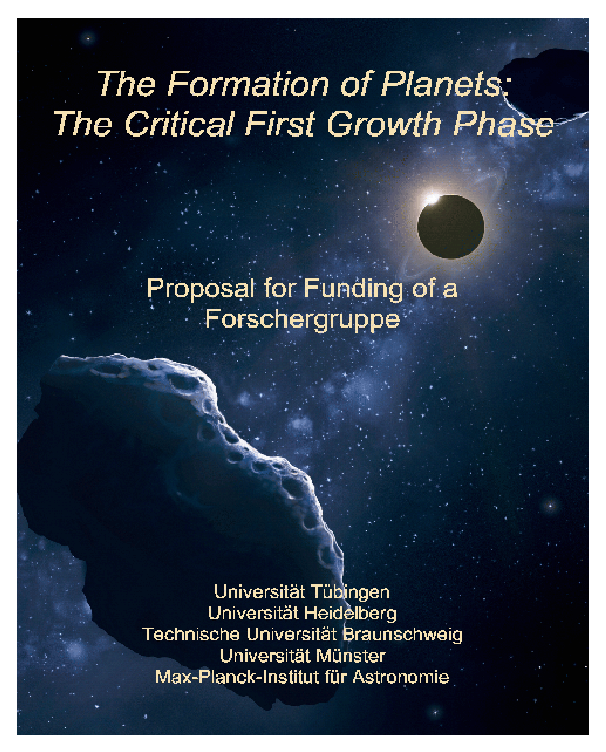
\includegraphics[width=16cm]{cover.eps}
\clearpage
\mbox{}
\vfill
\noindent{\it {\bf Front page image:} ``Beyond the Realm of
the Giants'' by Mark Garlick. This painting gives an artist's impression of
Kuiper belt objects in our solar system, which are left-overs from the
planet formation era. These icy objects are examples of the
``planetesimals'' at the center of this Forschergruppe. Since the painting
also shows some amounts of dust, this painting also symbolizes the process
of formation from dust to planetesimals.}
\clearpage
%
% Title page
%
\mbox{}
\vspace{4cm}\\
\centerline{\huge \bf Planet Formation Witnesses and Probes:}

\vspace{1cm}

\centerline{\huge \bf Transition Discs}

\vspace{3cm}

\centerline{\Large \bf Proposal for Funding of a Forschergruppe}

\vspace{3cm}

\centerline{\Large Speaker: B.~Ercolano}

\vspace{0.5cm}

\centerline{\Large Co-speaker: C.~P.~Dullemond}

\vfill
\mbox{}
%\pagebreak[4]
\cleardoublepage
\mbox{}
\centerline{\Large \bf Table of Contents}
\vspace{3em}\\

\newcounter{pgcntr}
%\begin{tabular}{p{5em}l}
%5   & Summary, Introduction and motivation
%
%\end{tabular}

\setcounter{pgcntr}{6}
\contentsline{section}{Overview over the Forschergruppe}{\arabic{pgcntr}}
\contentsline{subsection}{Participating institutes and principle investigators}{\arabic{pgcntr}}
\addtocounter{pgcntr}{1}
\contentsline{subsection}{Summary}{\arabic{pgcntr}}
\contentsline{subsection}{Introduction}{\arabic{pgcntr}}
\addtocounter{pgcntr}{3}
\contentsline{subsection}{Scientific background and own contributions}{\arabic{pgcntr}}
\addtocounter{pgcntr}{6}
\contentsline{subsection}{Scientific objectives}{\arabic{pgcntr}}
\addtocounter{pgcntr}{1}
\contentsline{subsection}{Work plan of the proposed Forschergruppe}{\arabic{pgcntr}}
\addtocounter{pgcntr}{8}
\contentsline{subsection}{Forschergruppe Professur}{\arabic{pgcntr}}
\addtocounter{pgcntr}{1}
\contentsline{subsection}{Financial overview}{\arabic{pgcntr}}
\addtocounter{pgcntr}{3}
\contentsline{subsection}{Signatures}{\arabic{pgcntr}}
\addtocounter{pgcntr}{1}
\contentsline{subsection}{References}{\arabic{pgcntr}}
\addtocounter{pgcntr}{8}
\contentsline{section}{Project descriptions}{\arabic{pgcntr}}
\addtocounter{pgcntr}{1}
\contentsline{subsection}{Project A1: ``Thermal annealing, evaporation, condensation''}{\arabic{pgcntr}}
\addtocounter{pgcntr}{22}
\contentsline{subsection}{Project A2: ``Mineralogical and chemical composition''}{\arabic{pgcntr}}
\addtocounter{pgcntr}{22}
\contentsline{subsection}{Project B1: ``Charge transfer''}{\arabic{pgcntr}}
\addtocounter{pgcntr}{16}
\contentsline{subsection}{Project B2: ``Influence of multiple collisions''}{\arabic{pgcntr}}
\addtocounter{pgcntr}{12}
\contentsline{subsection}{Project B3: ``High-temperature dust collision experiments''}{\arabic{pgcntr}}
\addtocounter{pgcntr}{16}
\contentsline{subsection}{Project B4: ``Simulating collisions with SPH''}{\arabic{pgcntr}}
\addtocounter{pgcntr}{12}
\contentsline{subsection}{Project C1: ``Planetesimal precursors in turbulent disks''}{\arabic{pgcntr}}
\addtocounter{pgcntr}{20}
\contentsline{subsection}{Project C2: ``Modeling dust coagulation''}{\arabic{pgcntr}}
\addtocounter{pgcntr}{20}
\contentsline{subsection}{Project D1: ``Radioisotope chronometry''}{\arabic{pgcntr}}
\addtocounter{pgcntr}{20}
\contentsline{subsection}{Project D2: ``Prediction of observable quantities''}{\arabic{pgcntr}}
\addtocounter{pgcntr}{20}
\contentsline{subsection}{Project P\hspace{0.7em}: Forschergruppe Professur}{\arabic{pgcntr}}
\addtocounter{pgcntr}{4}
\contentsline{subsection}{Project Z\hspace{0.7em}: Coordination}{\arabic{pgcntr}}
\addtocounter{pgcntr}{4}
\contentsline{section}{Curricula Vitae}{\arabic{pgcntr}}

\vfill

\clearpage
%
% Headers and footers for main text
%
\makeatletter
\newcommand{\hdrtitle}{Forschergruppe Planet Formation Witnesses and Probes:
Transition Discs}
%\newcommand{\hdrtitle}{XXXX}
\lhead[{\bfseries \hdrtitle}]{}
\rhead[]{{\bfseries \hdrtitle}}
\lfoot[\thepage]{}
\rfoot[]{\thepage}
\cfoot[]{}
%\setlength{\headrulewidth}{0.5pt}
\makeatother
%
% The main text
%
%
%   Main Text for  Forschergruppenproposal
%    The Formation of Planets
%         May 2006
%
\section{Participating institutes and 
principle investigators
%\footnote{Only PIs and Co-PIs listed. Co-investigators and 
%collaborators are listed in individual projects.}
}\label{app-institutes}
\vspace{0.1em}
\renewcommand{\hdrtitle}{Participating institutes and PIs}
\begin{itemize}
\item {\bf University of T\"ubingen:}
\begin{compactitemize}
  \item Institute for Astronomy \& Astrophysics \\
%%    Dept.~of Computational Physics \\
         {\em (Prof.~Dr.~W.~Kley, Dr.~R.~Speith)}
\end{compactitemize}
\item {\bf University of Heidelberg:}
  \begin{compactitemize}
  \item Institute for Theoretical Astrophysics\\
         {\em (Prof.~Dr.~W.~M.~Tscharnuter, Prof.~Dr.~H.-P.~Gail)}
  \item Mineralogical Institute \\
         {\em (Dr.~M.~Trieloff, Prof.~Dr.~D.~Lattard, Prof.~Dr.~R.~Altherr)}
  \item Kirchhoff Institute of Physics, group ``Surface Science and
         Infrared Spectroscopy of Nanostructures'' \\ {\em
         (Prof.~Dr.~A.~Pucci)}
  \end{compactitemize} 
\item {\bf Max-Planck-Institute for Astronomy, Heidelberg:}
\begin{compactitemize}
  \item Planet and Star Formation Group\\
         {\em (Dr.~H.~Klahr, Dr.~C.~P.~Dullemond, Prof.~Dr.~Th.~Henning)}
  \item Emmy Noether Group ``Evolution of circumstellar dust disks to
         planetary systems''\\
         {\em (Dr.~S.~Wolf)}
\end{compactitemize}
\item {\bf Technical University at Braunschweig:}
\begin{compactitemize}
  \item Institute for Geophysics and Extraterrestrial Physics \\
         {\em (Prof.~Dr.~J.~Blum)}
\end{compactitemize}
\item {\bf University of M\"unster:}
\begin{compactitemize}
  \item Emmy Noether Group ``Dust, Gas, Radiation and Planet Formation''\\
         {\em (Dr.~G.~Wurm)}
  \item Institute of Planetology\\
         {\em (T. Stephan)}
\end{compactitemize}
\end{itemize}
%
%\mbox{}\vspace{0.2em}\\
%
\noindent {\bf Speaker:}\\
%%\noindent Prof.~Dr.~W.~M.~Tscharnuter \hfill Tel.: 06221-544815\\
%%Zentrum f\"ur Astronomie, Uni-HD \hfill e-mail wmt@ita.uni-heidelberg.de\\
%Institut f\"ur Theoretische Astrophysik\\
%Universit\"at Heidelberg, \\
%%Albert-\"Uberle-Str. 2, D-69120 Heidelberg\\
%%  New since April 2006 
\noindent Prof.~Dr.~W.~Kley \hfill Tel.: 07071-29-74007\\
University of T\"ubingen \hfill 
E-mail: wilhelm.kley@uni-tuebingen.de\\
Institute for Astronomy \& Astrophysics \\
Auf der Morgenstelle 10, D-72076 T\"ubingen\\[1em]

\noindent {\bf Co-speakers:}\\
\noindent Dr.~C.~P.~Dullemond \hfill Tel.: 06221-528-395\\
Max-Planck-Institute for Astronomy\hfill 
E-mail: dullemon@mpia.de\\
K\"onigstuhl 17, D-69117 Heidelberg\\[0.1em]

\noindent Dr.~M.~Trieloff \hfill Tel.: 06221-546022\\
Mineralogical Institute \hfill E-mail: trieloff@min.uni-heidelberg.de\\
University of Heidelberg \\
Im Neuenheimer Feld 236, D-69120 Heidelberg


\pagebreak[4]


\section{Summary}
\renewcommand{\hdrtitle}{Summary}
The formation of planets is one of the key questions in astrophysics. The
first step in this process is the coagulation of dust: the growth from
sub-micron dust particles to ever larger aggregates ultimately leading to
the formation of multi-kilometer sized `planetesimals'. Once these
planetesimals are formed, gravitational interaction starts to dominate over
all other forces, and eventually leads to the formation of rocky planets.
In our proposed Forschergruppe we focus on the {\it first stage} in the planet
formation scenario, i.e. on the growth process from dust to planetesimals.
 
This stage suffers from a large number of
unsolved mysteries, many of which are critical to our understanding of the
planetesimal formation process as a whole.  
Among them are: The seemingly insurmountable
`meter-size barrier' for the collisional growth of particles, the poorly
understood causes of the complex mineralogical structure of meteorites, and
the apparent lack of correlation between certain observational signatures of
grain evolution and the age of the parent star. In spite of the clear
connection between these issues, they have mostly been studied by somewhat
separate scientific communities. In particular the
meteoritics/cosmochemistry/astromineralogy community, the collision
experimentalists, the theoretical astrophysicists and the observational
astronomers have had relatively little cross-field collaboration in the past. 
The most promising option to solve many questions surrounding the growth from dust to
planetesimals is to unite these various communities in a joint research
effort. This is the purpose of the proposed Forschergruppe.


\section{Introduction and motivation}
\renewcommand{\hdrtitle}{Introduction} Understanding the formation of
planets is of such importance because it relates to the foundation of our
own existence, and whether planets such as our Earth are rare or common in
the Milky Way. Although it is one of the oldest questions in astronomy and
of mankind, it has recently attained strong renewed interest stimulated by
the discovery of over 180 extrasolar planets around solar-type stars in the
last decade. Improved observational sensitivity has allowed to detect objects
as small as Neptune (14 Earth masses), and through transit observations
physical properties of extrasolar planets such as radius and mean density
have been inferred.  Moreover, with the newest infrared telescope
facilities, the birthplaces of planets - the dusty protoplanetary
circumstellar disks left over from the star formation phase - can now be
studied to an unprecedented level of detail, allowing astronomers and
astrophysicists to put theories of planet formation to the test. The near
future also promises interesting new views on this issue: it is expected
that within 10 years {\em earth-like} extrasolar planets will have been
discovered with space missions, which will put new constraints on the
scenarios of formation of planets such as our own.

Planet formation is believed to begin with the coagulation of dust in
protoplanetary disks, forming ever larger aggregates of solid material through
a sequence of collisions and agglomerations. This growth process 
continues until eventually these bodies become gravitationally bound
objects of a few kilometers in size. This initial phase of planet formation
constitutes a growth over 10 orders of magnitude in size and over 30 orders
of magnitude in mass. It is a process of high complexity involving many
aspects of physics, chemistry, astronomy and mineralogy. These aspects
include the physics of colliding aggregates, the internal structure of
aggregates, the solid-state chemistry of grains at high temperatures, the
interaction between grains and the surrounding gas and hydrodynamic flows,
and the large-scale evolution of dust populations. The study of these
processes also requires knowledge on the structure and evolution of the
disks in which these processes take place, including the transport of
radiation through these disks. Moreover, the evolving dust population has a
back reaction on the structure of these disks. A comprehensive study of the
growth process from sub-micron dust particles to multi-kilometer planetesimals is
therefore a problem of such complexity that its study requires a large
collaborative effort between scientists with expertise in all these various
mutually-interacting aspects of this problem.
 
%
\subsection{Why study {\em this} stage of planet formation?}
\label{subsec:whynow}
%
Although the {\em entire} process of planet formation is highly relevant,
the first stage --the growth from dust to planetesimals-- is of particular
interest. There are three main reasons for this: {\it 1)} 
This is probably the observationally best constrained part of the planet
formation theory, with a wealth of infrared and sub-millimeter data from 
hundreds of protoplanetary disks, and the additional detailed meteoritic knowledge of
our own Solar System. {\it 2)} This is the stage of planet formation that
links the origin of asteroids and comets to the origin of planets, and which
gives a comprehensive view on the formation of rocky planets. {\it 3)} 
It involves many unsolved critical questions about planet formation in areas of
expertise of our team.

Many of these questions are so fundamental that to this date there 
exists no standard scenario of how this process operates. For instance, it is
not known how particles survive the `meter-size barrier', a size-regime in
which relative velocities are so large that a collision with an equal-sized
body would completely destroy both objects. Moreover, according to simple
physical arguments, bodies of this size should drift very rapidly
towards the star, vaporize, and therefore get lost for the planetesimal
formation process. Even putting these issues aside, it is still not known
{\em how} bodies grow to planetesimal sizes. Is it a hierarchical growth
process, or do the biggest bodies grow by sweeping up large quantities of
dust and small bodies? Under which conditions are
these impacts constructive and when are they erosive?  Does the growth take
place everywhere in the whole disk, or does it require an essential
boost through some triggering mechanisms such as hydrodynamic clustering of
particles in vortices and/or turbulent eddies?

These are only a few of the fundamental unsolved questions concerning the
theory of particle growth and planetesimal formation.  When considering the
{\em composition} and size-distribution of these particles, as measured by
infrared observations of protoplanetary disks and (in even more detail) by
meteoritic studies of our own Solar System, one is confronted by an equally
puzzling --and similarly vast-- set of additional mysteries.  For instance,
it is a hotly debated issue why the elementary composition of chondrules -
millimeter sized crystalline globules of which chondritic meteorites are
largely built up - is complementary to that of the fine grained matrix
particles between chondrules, and what is the reason for compositional
variety of chondrite parent bodies.  Furthermore, it is unclear why
Calcium-Aluminum-rich Inclusions (CAIs) are a few million years older than
most chondrules from the same meteorites, and why differentiated meteorites
are nearly as old as CAIs and hence, older than chondrites and
chondrules. The composition of comets is also enigmatic - though there are
likely cometary particles (fluffy, anhydrous) in collected interplanetary
dust samples, it is unclear, why these contain mostly isotopically normal,
solar dust. Here, soon progress is expected by the Stardust mission.  Also
from observations of protoplanetary disks there are many puzzles, for
instance: why do signatures of grain growth and thermal processing
(crystallinity) not appear to be correlated with the stellar age? Is there
another parameter in addition to stellar age?
%

\subsection{Why study it {\em now}?}
%
Three recent ground-breaking new developments have improved our
understanding of this topic, and are major motivations for the
Forschergruppe:

\noindent {\it 1)} There is enormous progress in infrared astronomy, in
particular in the spectroscopic study of dust particles in protoplanetary
disks around Herbig Ae/Be stars, T Tauri stars, and Brown Dwarfs. For many
years the Hubble Space Telescope has provided us with outstanding images and
spectra, and since 2004 the {\em Spitzer Space Telescope} yields enormous
quantities of data on the dust grain sizes and composition in infant `Solar
Systems'. Its unprecedented sensitivity allows, for the first time, a
detailed look at the infrared spectra of dim sources such as T Tauri stars
(among which are infant sun-like stars) and even Brown Dwarfs. Moreover, the
sample of sources with good spectra has increased dramatically with this
telescope, so that detailed statistical studies can be done. In addition to
this, since 2003 the Very Large Telescope (ESO, Chile) can spatially resolve
the very inner regions of protoplanetary disks where Earth-like planets may
form, and analyze grain sizes and composition as a function of distance from
the star down to spatial scales of about 1 AU.  And finally, in recent years
there have been major breakthroughs in millimeter interferometry
measurements of protoplanetary disks. With these measurements it has been
established that large quantities of few-millimeter sized pebbles reside in
the midplane of these disks out to many tens of astronomical units, posing
problems to theories of grain motion. Moreover, sometimes this mm/cm size
grain population can been shown to have a very narrow size distribution,
which is a puzzle for theoretical models.
%  The Max Planck Institute for Astronomy
% (MPIA) in Heidelberg has a large team of scientists working on the analysis
% of these data in order to gain insight on the growth and thermal/chemical
% processing of dust grains in protoplanetary disks.

\noindent {\it 2)} 
In recent years there has been major progress in
laboratory experiments of collisions of dust aggregates. With these
experiments our knowledge of the sticking coefficients, the structure of
aggregates, and the typical (debris-) products of collisions are now much
better known than a decade ago. These microphysical data are the basic
physical ingredients for models dealing with the evolution of the grain size
distribution in protoplanetary disks. New and improved coagulation models
can therefore be developed based on these data, and the above mentioned
questions can be addressed with more reliable and realistic tools.
% The Laboratories in Braunschweig and M\"unster have played a major
% role in these developments.

\noindent {\it 3)} 
The last decade brought enormous progress in micro- and
nano-analytics of extraterrestrial matter and advances in establishing the
chronology of early Solar System processes, particularly regarding the
growth of asteroid-sized planetesimals.
%
The STARDUST mission - the first sample return mission since the Apollo
program - just brought back cometary dust from comet Wild-2. The analysis of
this most primitive matter has started and is expected to significantly
increase our knowledge about the formation of the first small bodies in our
solar system.
%
It is tantalizing to compare what we
know from our own Solar System with results from infrared observations of
protoplanetary disks, and to try to match theories of grain growth to these
observations. In this way, both our own Solar System, as well as
proto-solar-systems in our neighborhood may be able to provide new clues to
the growth of planetesimals.



\subsection{Why do we need a Forschergruppe?}
%
The problem of the formation of planetesimals involves many different
processes which are often studied by very different communities. While the
formation of our own Solar System is studied by meteoritic scientists, the
observations of protoplanetary disks are performed by observational
astronomers. And while the collisions of aggregates are studied in the lab
by laboratory astrophysicists, the mineralogical composition of these grains
is studied by cosmochemists.
%
% KEES: Cosmochemists?
%

Yet, it is evident that all these aspects are strongly intertwined. Each of
these aspects has so far been studied mostly in isolation, but this was
only possible because drastic simplifying assumptions have been made for the
other aspects. For instance, the materials used for aggregates in laboratory
collision experiments were mostly quartz spherules, while we know that a
whole variety of different minerals must have been present in the early solar nebula.
Models of grain growth often use a relatively primitive coagulation kernel,
while lab experiments have demonstrated its immense
complexity. Interpretation of infrared observations often employs models
with simple power-law grain size distributions, while theory clearly shows
that grain size distributions differ substantially from a power-law.

{\em Only by studying all aspects in a unified way there is hope that real
progress can be made, and the main unexplained problems be solved.} Since
isolated research efforts cannot cover all these aspects, it is clear that
such a study requires a close collaborative project involving experts from
all these aspects of planetesimal formation. The initiation of such a joint scientific
effort combining different research fields is one of our main goals to achieve
with this Forschergruppe. 

%\pagebreak[4]

\section{Scientific background and own contributions}
\renewcommand{\hdrtitle}{Scientific background}
%
In the following subsections we will summarize the state of the various
areas of research mentioned in the introduction and own contributions in these.

\subsection{Disk structure and evolution:}
%
Though disk structure and evolution is not the topic of this Forschergruppe,
the physics of planetesimal formation takes place within such disks. For
this reason our expertise on this topic plays an important role in this
Forschergruppe, and we will concisely list our contributions to this field
below.  But since this field is quite extensive, and not within the main
focus of this Forschergruppe (it only plays a passive supportive role), we
do not review the current status of this field here. For recent reviews see
e.g.~D'Alessio et al.~(\cit{2005}) and Dullemond et al.~(\cit{2006}).

\paragraph{Our contributions:}
%
The detailed 2-D global structure of irradiated protoplanetary disks has
been studied by Dullemond et al.~(\cit{2002, 2003, 2004b}).  Hydrodynamic
and radiative transfer models for disks are also available within the group
of Gail \& Tscharnuter (Gail \cit{2001, 2003, 2004}; Wehrstedt \&
Gail \cit{2002, 2003}), as well as in the groups of Klahr and Henning (Bell
et al.~\cit{1997}; Klahr et al.~\cit{1999, 2003, 2005}; W\"unsch et
al.~\cit{2005}) and of Kley (Kley et al.~\cit{2001}; G\"unther et
al.~\cit{2002, 2004}; Sch\"afer et al.~\cit{2004}). Models of the ionization
of disks, with particular relevance to the magneto-rotational instability,
have been constructed by Semenov \& Henning (\cit{2004}).  Models of the
formation and viscous evolution, based on time-dependent $\alpha$-disk
equations, were published by Dullemond et al.~(\cit{2006a}, \cit{2006b}).


\subsection{Thermal processing and radial mixing}
%
Cometary nuclei contain ices, refractory organics and silicate dust grains
(Jessberger et al. 1988; Jessberger 1999). Recent observations made clear
that, in addition to amorphous dust, such comets also contain a considerable
fraction of crystalline Mg-rich silicate dust species (e.g.\ Wooden et
al.~\cit{1999, 2000, 2004}). Such dust species are can only be created at
temperatures exceeding 800 K. The coexistence of this high temperature
material with amorphous dust in the same objects points to large scale
radial mixing/transport processes in protoplanetary disks
(e.g.~Bockel\'ee-Morvan et al.~\cit{2002}; Nuth \& Johnson \cit{2006}),
although shocks have also been discussed (e.g.\ Harker \& Desch \cit{2002};
Miura \& Nakamoto \cit{2005}). Such processes are important for the disk
structure and its material, as well as for the composition of the planets
and planetesimals formed in the disk (e.g.~Morfill, Tscharnuter \& V\"olk
\cit{1985}).

Crystalline silicate dust is also detected in protoplanetary disks
(e.g.~Meeus et al.~\cit{2001}; Bouwman et al.~\cit{2001}; Apai et
al.~\cit{2005}). For three such sources, the 'Mid-Infrared Interferometric
Instrument' (MIDI) has recently obtained mid-infrared spectra of the disk at
different stello-centric radii (\coll{van Boekel et al.~\cit{2004}}).  These
observations clearly show a radial decrease of the degree of crystallization
of the dust in the disk, which points to radial mixing theories. But it
remains a puzzle why some sources have significantly more crystalline dust
than others. 
% {\bf [****** STATEMENT REMOVED ******]}
%, and how it can be that some sources appear to have virtually no
%crystalline silicates just outside of the thermal annealing radius (indicating
%zero mixing).

%\remark{INSERT EVAPORATION CONDENSATION}
Besides the crystallinity of the dust, thermal processes also govern the
composition of dust or the abundance of distinct mineral species via
evaporation/condensation processes and solid-gas phase chemistry. This also
influences the bulk chemical composition of solids at certain radial
distances, and is a possible source of compositional variety of chondritic
and other planetary bodies (Palme \cit{2001}). Modeling of annealing and
evaporation/condensation processes needs experimental data. However,
existing data mainly focussed on forsterite and enstatite (e.g.\ Hallenbeck
et al.~\cit{1998}; Brucato et al.~\cit{1999}; Fabian et al.~\cit{2000};
Thompson et al.~\cit{2002}; Hashimoto~\cit{1990}; Nagahara et
al.~\cit{1994}; Tsuchiyama et al.~\cit{1999}; Wang et al.~\cit{1999}; Mysen
\& Kushiro~\cit{1988}; Tachibana et al.~\cit{2002}), but do not cover the
whole range of mineral species that must be taken into account (e.g.
Fe-bearing olivine, pyroxene, Ca-Al minerals, or minerals accommodating
moderately volatile elements).


\paragraph{Our contributions:} 
%
Quantitative model calculations for thermal annealing and radial mixing have
only recently be performed by Gail (\cit{2001, 2004}), Wehrstedt \& Gail
(\cit{2002, 2003}) and in a simplified form by Bockel\'ee-Morvan et
al.~(\cit{2002}) and Dullemond et al.~(\cit{2006}). These studies have shown
that radial mixing of chemically and thermally processed (annealing,
vaporization and re-condensation) material from warm inner disk regions into
the comet forming regions of the accretion disk can explain the existence of
significant amounts of crystalline silicate dust in comets. Large scale,
multi-dimensional circulation currents can also play an important role in
this process (e.g.\ Kley \& Lin \cit{1992} and \team{Keller \& Gail
\cit{2004}}). Johansen \& Klahr (\cit{2005}) and Johansen, Klahr \& Mee
(\cit{2006}) have measured the Prandtl
numbers for vertical and radial mixing in 3D-MHD simulations, which is 
input to radial mixing models. The group of
Henning performed laboratory measurements that are compiled in a
spectroscopy database (\cit{1999}), and they also issued the first book on
Astromineralogy (\cit{2003}).

%
\subsection{Collisions between aggregates}
%
The growth of particles in protoplanetary disks is driven by collisions.
These collisions are due to Brownian motion, drift motions relative to the
gas, and gas turbulence, respectively (V\"olk et al.~\cit{1980};
Weidenschilling \& Cuzzi \cit{1993}). There has been a long debate as to
under which circumstances dust particles stick to each other in such
collisions.  Models of dust motion in protoplanetary disks predict that the
relative velocities between the aggregates increase with increasing mass
(Weidenschilling \& Cuzzi \cit{1993}). Experiments on the sticking
efficiency of micrometer-sized spherical polystyrene particles showed that
these particles stick whenever they collide with velocities smaller than
$\approx 1$ m/s (Dahneke \cit{1975}). Chokshi et al.~(\cit{1993})
developed a collision model for spherical dust particles whose energy loss
was mainly due to the excitation of elastic surface waves. This model fits
the data from Dahneke (\cit{1975}) for the rather ``soft'' polystyrene
particles but later proved to underestimate the threshold velocity for
sticking for more realistic (``harder'') particle materials (Poppe et
al.~\cit{2000a}).  Another important factor is the porosity and/or fractal
structure of aggregates, due to the dramatic differences in collision and
aerodynamic cross sections (Meakin \& Donn \cit{1988}; Weidenschilling
\cit{1990}).  The formation of fractal dust aggregates was studied in
detail by Ossenkopf (\cit{1993}) and Kempf et al.~(\cit{1999}), and the
physics of fractal-aggregate collisions was modeled by Dominik \& Tielens
(\cit{1997}).  The latter authors found that at velocities above a certain
threshold aggregate compaction, grain losses and aggregate fragmentation
come into play. This was later confirmed experimentally (Blum \& Wurm
\cit{2000}). Impact, collision, and aggregation experiments from groups
not involved in the Forschergruppe and with immediate relevance to the
formation of planetesimals are scarce. Praburam \& Goree
(\cit{1995}) produced fluffy dust aggregates in a plasma environment, but
the application of this to the relatively plasma-free protoplanetary nebula
is questionable; Nuth et al.~(\cit{1994}) performed experiments with
magnetic iron dust grains, but the role of magnetic grains for planetesimal
formation is unclear; Hatzes et al.~(\cit{1991}), Bridges et
al.~(\cit{1996}) and Supulver et al.~(\cit{1997}) investigated the
``stickiness'' of macroscopic icy bodies; while Kouchi et al.~(\cit{2002})
performed collision experiments with centimeter-sized particles covered by a
millimeter-thick organic substance. Most of these experiments and models
were focused on particles of micron size up to a few decimeter in
size. Smooth Particle Hydrodynamical model calculations of collisions of
bigger bodies were performed by Benz et al.~(\cit{2000, 1994}). These
techniques were used by Sirono (\cit{2004}) and Sch\"afer et
al.~(\cit{2005}) to model ruptures in (icy) dust aggregates.


\paragraph{Our contributions:}
%
The experimental groups in Braunschweig and M\"unster (both originally
coming from Jena) have performed a multitude of laboratory and space
experiments on dust-dust interactions.  General studies include Poppe et
al.~(\cit{2000a}), Heim et al.~(\cit{1999}). We have studied in detail the
formation of fractal aggregates (Blum et al.~\cit{2000}; Krause \& Blum
\cit{2004}; Blum et al.~\cit{1999}; Wurm \& Blum \cit{1998}). We have shown
that above a critical aggregate mass, that depends on the friction forces
between contacting dust grains (\team{Heim et al.~\cit{1999}}), collisions
lead to the compaction of the dust aggregates (Dominik \& Tielens
\cit{1997}; Blum \& Wurm \cit{2000}), and produce aggregates with a porosity
of 65\% or higher (\team{Blum \& Schr\"apler \cit{2004b}; Blum
\cit{2004}}). Above a certain impact velocity, the colliding dust aggregates
(with typical sizes of decimeter to meter) are no longer able to stick to
each other: the larger of the two colliding bodies is eroded while the
smaller one is fragmented (Wurm et al.~\cit{2005b}). One of the suggestions
to overcome this problem is based on earlier laboratory work on grain
charging (Poppe et al.~\cit{2000b}; Poppe \& Schr\"apler \cit{2005}). The
accumulation of charges on larger protoplanetary bodies can lead to the
re-attraction of smaller, oppositely-charged fragments after an impact (Blum
\cit{2004}). Another idea is based on the finding that for compacted dust
targets a considerable fraction of the impinging dust-projectiles stuck to
the target when the impact velocities were above $\sim 10$ m/s (\team{Wurm
et al.~\cit{2005b}}). Impact compaction, sintering, and eutectic melting are
the most promising processes to increase the strength of protoplanetary
bodies. Numerical models of coagulation were done by our team (Kempf et
al.~\cit{1999}), and Sch\"afer et al.~(\cit{2005}) performed numerical
modeling of impacts and collisions of larger, porous bodies, utilizing a
detailed elasto-plastic model for the projectile and target. These
simulations have used the Smooth Particle Hydrodynamics (SPH) method.

% There are several ideas how loose dust aggregates might
% become more rigid and, hence, might be able to grow beyond the meter-size
% limit. Impact compaction, sintering, and eutectic melting are the most
% promising processes to increase the strength of protoplanetary bodies and,
% thus, reduce their sensitivity to impact erosion. Dedicated experimental
% work to test the above hypotheses for the formation of large dust aggregates
% are required and shall be executed within this Forschergruppe.



\subsection{Coagulation and sedimentation of dust}
%
The growth from sub-micron sized dust grains to a single multi-kilometer
sized planetesimal involves well over $10^{30}$ individual 
collisions events. While individual
collisions can be studied in laboratory experiments and SPH simulations (see
above), the overall evolution of the particle population throughout the disk
can only be understood using numerical models based on particle distribution
functions.  Such models are heavily dependent on the input physics at the
smallest scales, such as the sticking properties, the binding energy of the
grains, the cross-section of these grains, and the typical outcome of
collisions. The first models for the evolution of particle distribution
functions were made by Weidenschilling et al.~(\cit{1980}) and Nakagawa et
al.~(\cit{1981}), though with very limited computing power. Further work has
been done by e.g.~Nakagawa et al.~(\cit{1986}), Mizuno et
al.~(\cit{1988, 1989}) and Weidenschilling (\cit{1984, 1997}). The
back-reaction on the disk evolution was studied by Morfill (\cit{1988}),
Schmitt et al.~(\cit{1997}) and Suttner \& Yorke (\cit{2001}).  Recently,
Dullemond \& Dominik (\cit{2005}) and Tanaka et al.~(\cit{2005}) studied the
effects of coagulation on the observational appearance of disks.

One of the main problems of the above sketched scenario is that once
particles become larger than about 1 meter (at 1 AU), the relative velocity
between them becomes so large that collisions will be destructive. Also,
radial drift has its maximum at that particle size (e.g.~Weidenschilling
\cit{1997}), and consequently such particles quickly drift toward the star
and vaporize. It is not known how particles can overcome this `meter-size
barrier' and grow to sizes where both drift and destructive collisions are
no longer a problem. An alternative scenario is therefore often
discussed. If the disk is quiescent (non-turbulent), dust grains are allowed
to sediment to the midplane, forming a thin midplane layer. Goldreich \&
Ward (\cit{1973}) argued that such a midplane layer can become
gravitationally unstable, fragment and form planetesimals. However,
Weidenschilling (\cit{1980}) and Cuzzi et al.~(\cit{1993}) argued that the
tiny amount of turbulence caused by the shearing layer prevents the layer
from becoming thin enough for instability. Recent work by Youdin \& Shu
(\cit{2002}) suggests solutions to this problem, but this work is still
actively debated.


\paragraph{Our contributions:}
%
As pointed out above, we have been involved in the study of the
back-reaction of dust growth on the evolution of the disk (Schmitt, Henning
\& Mucha~\cit{1997}). The radial drift of growing bodies, and the
consequences thereof, have been studied recently by Kornet et
al.~(\cit{2001}). In the context of the discussion of the Goldreich-Ward
instability, we derived more detailed expressions for the sedimentation
velocity of grains in disks, and studied the instability itself (Schr\"apler
\& Henning \cit{2004}; Johansen, Henning \& Klahr \cit{2006}).  We performed
self-consistent model calculations of the effect of grain coagulation
(modeled using distribution functions) on the infrared spectra of
protoplanetary disks (Dullemond \& Dominik \cit{2005}).  Also, in an earlier
paper, the effects of sedimentation were investigated in this way (Dullemond
\& Dominik \cit{2004}), and it was concluded that the distinction between
two main classes of observed disks can be explained by sedimentation.


\subsection{The dynamic coupling of dust and turbulence}
%
Dust grains in protoplanetary disks are subject to radial drift as well as
vertical sedimentation (Whipple \cit{1972}; Weidenschilling \& Cuzzi
\cit{1993}). Turbulence, which appears to play a crucial role in the
accretion process (Balbus \& Hawley \cit{1998}), most likely plays a pivotal
role in the dust coagulation process (e.g.~V\"olk et al.~\cit{1980}; Mizuno,
Markiewicz \& V\"olk \cit{1988}).  Turbulence can segregate and concentrate
dust grains in vortices (Barge \& Someria \cit{1995}), in convection cells
(\team{Klahr \& Henning \cit{1997}}) and, through turbulence, in either the
regions between the eddies (Cuzzi et al.~\cit{2001}) or in the center of
those (\team{Johansen \& Klahr \cit{2005}}).
%
Turbulence is also important in producing relative velocities between
grains, which is necessary for grains to collide and stick to each other
(Weidenschilling \& Cuzzi \cit{1993}). For equal sized boulders turbulence
is the only source for relative velocities by producing an r.m.s.\ velocity
among the grains (Markiewicz \cit{1991}).
%
The turbulence also has significant consequences for the observed structure
of the disk: small grains sediment barely, because they get stirred up by
the turbulent gas, while big grains form a thin midplane layer well below
the disk infrared-photosphere and only become visible in the sub-millimeter.


\paragraph{Our contributions:}
%
We have investigated a very general trapping mechanism for grains in a gas
flow.  Dust grains tend to drift into regions of maximum gas pressure
(\team{Klahr \& Lin \cit{2001, 2005}}) which explains
not only trapping but also radial drift as well as vertical sedimentation.
The interaction of turbulent and non-turbulent parts of the solar nebula has
been studied (\team{W\"unsch, Klahr \& R\'o\.zyczka
\cit{2005}}). Johansen, Andersen \& Brandenburg (\cit{2004}) have
investigated the trapping of dust in vortices including the feedback of the
dust onto the vortex. Klahr \& Bodenheimer (\cit{2006}) discuss the beneficial
action of a vortex for planet formation and derive relevant time scales.
Klahr \& Henning (\cit{1997}) discovered that convection cells can also
concentrate particles. Turbulent eddies have the property to trap dust at
least temporarily (\team{Johansen \& Klahr \cit{2005}}).

Turbulence also slows down the radial drift of meter sized boulders
(\team{Johansen, Klahr \& Henning \cit{2006}}). On large scales
turbulence acts as a diffusion process by transporting grains radially and
vertically (\team{Johansen \& Klahr \cit{2005}}).  Thus turbulence can
also work against infinite sedimentation of the solid particles toward the
midplane: the turbulence stirring will set a minimum limit to the geometric
thickness of a dust sub-disk for any given grain size. This can prevent the
disk from quickly forming planetesimals by gravitational instability of the
type of Goldreich \& Ward (\cit{1973}). Johansen, Henning \& Klahr
(\cit{2006}) have modeled this in time-dependent hydrodynamic simulations,
and confirmed this, but at the same time showed that strong
clumping can result in this dust layer.
For equal sized boulders we were able to measure relative velocities
(r.m.s.\ velocity) among meter sized objects directly from turbulence
simulations (\team{Johansen, Klahr \& Henning \cit{2006}}).


\subsection{Formation and chemical composition of small solar system bodies}
%
The origin of our own Solar System as evaluated by cosmochemistry is known
in surprising details (for recent reviews see e.g.~Lauretta et
al.~\cit{2006}; Krot et al.~\cit{2005}; Sears \cit{2004}; \team{Trieloff \&
Palme \cit{2006}}). Primitive extraterrestrial matter from small bodies
tells us about conditions and time scales of how dust grains formed and
aggregated to larger bodies, which then accreted to multi-km-sized
planetesimals. The first solids to condense were up to cm-sized Ca-Al-rich
inclusions (CAIs) (Amelin et al.~\cit{2002}) enriched in $^{16}$O (Clayton
et al.~\cit{1993}). Other high temperature products are mm-sized solidified
melt droplets called chondrules. Most chondrules formed 2-3 Myr later than
CAIs (Russell et al.~\cit{1996}; Kita et al.~\cit{2004, 2000}) and were
compacted rapidly together with fine-grained material formed at low
temperatures (chondrite "matrix") to km-sized planetesimals, probably within
$<$1Myr (see above quoted reviews). Most likely, due to pressure and
temperature differences imposed by the early sun, formation conditions of
minerals and chondritic asteroids varied with radial distance and/or
time. Differing proportions of refractory minerals and inclusions (CAIs,
forsterites), Mg-silicates, metal and minerals with volatile compounds
caused the compositional variety of chondritic planetesimals (Palme 
\cit{2001}). Radiometric dating using U-Pb-Pb (Amelin et al.~\cit{2002}),
$^{26}$Al-$^{26}$Mg (Bizzarro et al.~\cit{2004}; Russell et al.~\cit{1996};
Kita et al.~\cit{2000}; Zinner \& G\"opel \cit{2002}), $^{129}$I-$^{129}$Xe
(Gilmour et al.~\cit{2004, 2006}; Brazzle et al.~\cit{1999}), $^{53}$Mn-$^{53}$Cr
(Lugmair \& Shukolyukov \cit{1998}) and chemical composition suggest that
individual planetesimals formed over a time
interval of a few million years, but  individual planetesimals grew rapidly in the
asteroid belt, probably within $<$1Myr.
The exact chronology of meteorite parent body formation is vividly
debated, a recently suggested scenario is: Early planetesimals were heated
to varying degrees by decay heat of short-lived nuclides, primarily
$^{26}$Al (\team{Trieloff et al.~\cit{2003}}). This might have caused
melting and differentiation in early (within $<$2 Myr after CAIs) formed
planetesimals, leading to the formation of iron cores and basaltic rocks
(Kleine et al.~\cit{2005}), while planetesimals that accreted later remained
undifferentiated chondritic parent bodies (\team{Trieloff \& Palme
\cit{2006}}). As most chondrules were immediately consumed in accreting
planetesimals, they were only preserved in unmelted chondritic parent bodies
and their age distribution is biased to the formation time interval of
chondrites about 2--4 million years after CAIs. Several lines of evidence
suggest that part of accretion took place under conditions of enhanced
dust/gas ratios (see reviews quoted above), or during dispersal of disk gas
(\team{Trieloff et al.~\cit{2000, 2002}}). These constraints are important
for disk and coagulation models.
 
Our knowledge about chemistry and formation history of the 2nd major class
of small bodies in our solar system - comets - relies on remote observations
(Wooden et al.\ 1999, 2000, 2004) or in situ missions as to comet Halley
(Jessberger et al. 1988) or recently the Deep Impact mission to comet
9P/Tempel 1 (Harker et al.\ 2005). Significant advance can be expected due to
the STARDUST mission. Here, for the first time dust samples of unequivocally
cometary origin will be analyzed by laboratory high precision techniques
(Brownlee et al.\ 1996).

\paragraph{Our contributions:}
%
Trieloff et al.~(\cit{2000, 2002}) identified solar-wind-derived Neon in
Earth�s interior, implanted during an early stage of terrestrial accretion,
constraining the timing of accretion and disk gas dispersal. Trieloff et
al.~(\cit{2003}) determined high precision thermo-chronology of the H
chondrite asteroid and demonstrated that heating of the
planetesimals/asteroids in the early Solar System was caused by decay energy
of short-lived nuclides (e.g.\ $^{26}$Al). \team{Trieloff \& Palme
\cit{2006}} reviewed early Solar System processes and constructed a
time-scale of $^{26}$Al -heating that implies early formation of more
strongly heated asteroids.
%
T.\ Stephan is member of four sub-teams of the STARDUST preliminary
examination team, and has experience in the analysis of extraterrestrial dust
samples (Stephan et al.\ 1994, 2001, 2005).

%
\subsection{Observations of protoplanetary disks}
%
Most of the observable radiation from protoplanetary disks is caused by
thermal emission from the embedded dust grains. Upon growth their optical
properties change, and by studying the type, shape and strength of observed
infrared emission features from these sources, it is possible to draw
conclusions about the size distribution and mineralogical composition of the
grains (Bouwman et al.~\cit{2000}; Honda et al.~\cit{2003}; Przygodda et
al.~\cit{2003}; Kessler-Silacci et al.~\cit{2005, 2006}). These observations
have shown that the dominant grain size varies from source to source, which
suggests that these sources have been spotted at different stages in their
grain growth phase. However, there appears to be no correlation between this
typical grain size and the age of the star (van Boekel et al.~\cit{2005}).
There does, however, appear to be a correlation between grain size and
crystallinity (van Boekel et al.~\cit{2005}), but this is not yet well
understood.

The Spitzer Space Telescope, with its unprecedented sensitivity, is likely
to shed new light on these issues. This telescope is yielding spectra for a
much larger sample of stars than was possible before, and with much higher
quality (e.g.~Kessler-Silacci et al.~\cit{2006}). And techniques of infrared
interferometry now allow a view of the very inner regions of these dusty
protoplanetary disks (e.g.~Monnier et al.~\cit{2005}; Eisner et
al.~\cit{2003}; Leinert et al.~\cit{2004}).  There are also major
developments at sub-millimeter to centimeter wavelengths. For instance, the
midplane grain size can be estimated on the basis of (sub-)millimeter and
centimeter wavelength interferometry (e.g.~Testi et al.~\cit{2003}; Rodmann
et al.~\cit{2006}; Wilner et al.~\cit{2005}).
%

%
\paragraph{Our contributions:}
%
The group of Henning has provided comprehensive spectroscopy data for
researchers in Astronomy \& Astrophysics (Henning et al.~\cit{1999}).  The
Max Planck Institut f\"ur Astronomie in Heidelberg is involved in many
observational efforts and instrument developments, e.g.\ the MIDI
instrument, the only instrument worldwide for mid-infrared
interferometry. It is capable of probing dust composition and size in
earth-forming regions of protoplanetary disks. Using MIDI we showed that
crystallinity is stronger in the inner regions of the disk than in the outer
regions (van Boekel et al.~\cit{2004}).  Other relevant papers on MIDI
observations of protoplanetary disks are e.g.~Leinert et al.~(\cit{2004}),
Gil et al.~(\cit{2005}).  Furthermore, the Max-Planck-Institute for
Astronomy (MPIA) has strong involvement in
Spitzer data (e.g.~Silverstone et al.~\cit{2005}; Kim et al.~\cit{2005};
Hines et al.~\cit{2006}) and millimeter wave observations of
protoplanetary disks (e.g.~Carpenter et al.~\cit{2005}; Rodmann et
al.~\cit{2006}; Semenov et al.~\cit{2005}). The analysis of observations
at all wavelength is best done using detailed radiative transfer models, a
field in which our team has extensive experience.  For example, Wolf et
al.~(\cit{2003}) used such techniques to show that grains in the infalling
envelope in the Butterfly nebula are small while those in the disk of this
source are large (see also Wolf et al.~\cit{1999, 2003b}). We also
initiated the first 2-D continuum radiative transfer benchmark test project
(Pascucci et al.~\cit{2004}).  We were also the first to obtain infrared
and (sub-)millimeter data for a Brown Dwarf and present a corresponding disk
model (Pascucci et al.~\cit{2003}; Klein et al.~\cit{2003}).


%\pagebreak[4]

\section{Scientific Objectives}
\renewcommand{\hdrtitle}{Scientific Objectives}
The main goal of this Forschergruppe is 
to formulate and create a coherent picture of
the various processes that lead to the
formation of planetesimals, and to determine their structure and composition.
For this purpose we focus in the Forschergruppe specifically on a joint effort
and combine expertise from different scientific disciplines. 
For convenience, we shall formulate the scientific questions along the dividing lines
of the various fields, but their answers most likely lie (and shall be
sought) in the combination of these fields:
\makeatletter
\renewcommand{\theenumi}{\Alph{enumi}}
\renewcommand{\labelenumi}{\theenumi.}
%\renewcommand{\theenumii}{\roman{enumii}}
%\renewcommand{\labelenumii}{\theenumii}
\makeatother
\begin{enumerate}
\item {\bf What is the chemical/mineralogical composition of dust aggregates
  and planetesimals?}\\ How can we explain the variable planetary/chondritic
  compositions in our Solar System by means of evaporation, condensation and
  radial mixing of the most common minerals (Ca,Al minerals, Mg silicates,
  metal)? Can annealing experiments coupled with radial mixing models
  explain the observed crystallinity in protoplanetary disks, or are
  additional processes at work (e.g.~shock heating)?
\item {\bf What are the conditions under which collisions lead to growth?}\\
  How can solid bodies grow beyond about 1 meter in size, without getting
  destroyed through high-speed impacts? Does re-accretion of material after
  impact play a role, either by hydrodynamical interaction with the
  ambient gas or by charging upon impact?
  How does the composition of the materials affect the outcome of the
  collisions? Does thermal processing play a role (e.g.~sintering)? How does
  porosity develop in growing planetesimals?  Can collisions compactify
  bodies, and are such collisions required for further growth?  How do
  laboratory collision results scale with the size of the colliding objects?
%  \remark{MORE TEXT HERE: most of projects in this block!}
\item {\bf What is the large scale evolution of the dust population in size
  and location in the disk?}\\ How do the answers to A and B (and earlier
  research results in these areas) affect the grain size distribution in
  disks, and thereby the eventual formation of planetesimals? What is the
  main mode of growth to planetesimals: is it hierarchic (collisions between
  equal sized objects), or do big objects sweep up the smaller
  ones? How do dust inhomogeneities and concentrations in turbulent flows
  affect planetesimal formation (again in the light of the results of A and
  B)? How are particles transported in such turbulent disks?
  Does gravitational instability occur and does
  it lead to planetesimal formation?
\item {\bf How do the models compare to observations of our Solar System and
  of protoplanetary disks?}\\ Do coagulation and chemical models
  (i.e.~results from C and A) correctly predict the particle size
  distribution and mineral compositions of the dust observed in
  protoplanetary disks, and what can we learn from this? 
%  Does planetesimal formation lead to observable quantities? 
Are the timescales
  of planetesimal formation inferred from radiochronometry compatible with
  these models? Can we explain why grain growth/crystallinity signatures
  from infrared spectra of disks do not appear to correlate with stellar
  age? How does the Solar System compare to protoplanetary disks?
\end{enumerate}
\makeatletter
\renewcommand{\theenumi}{\arabic{enumi}}
\renewcommand{\labelenumi}{\theenumi.}
%\renewcommand{\theenumii}{\roman{enumii}}
%\renewcommand{\labelenumii}{\theenumii}
\makeatother


%\pagebreak[4]

\section{Work plan of the proposed Forschergruppe}
\renewcommand{\hdrtitle}{Work plan}
%
\subsection*{\em Overview over the Forschergruppe}
%%\noindent{\bf \em Overview over the Forschergruppe}\vspace{0.8em}\\
%
We intend to address the above questions by a combination of laboratory
experiments, theoretical modeling and a link to observations. A particularly
strong emphasis is put on the close collaboration between laboratory
experiments and theoretical modeling. On the one hand, laboratory
experiments provide physical parameters necessary as input physics of
certain theoretical models. On the other hand, theoretical models can be
directly compared to experiments, to explain the experimental results and to
test the validity of the models so that they can be extrapolated in size and
time-scale regimes beyond the reach of the laboratory.

A pivotal feature of this Forschergruppe is its {\em interdisciplinary character}.
We wish to combine, for the first time in such a systematic way, research of
dust mineralogy/chemistry, experimental and theoretical studies of aggregate
collisions, hydrodynamical models of particle-gas interactions, models of
dust coagulation, and observations (of protoplanetary disks and our own
Solar System).

The Forschergruppe consists of projects that are, from the start, designed
to be strongly inter-linked (see Fig.~1 and project descriptions). 
%
% This
% allows the participating scientists to replace the simplifying assumptions
% used so far by more detailed knowledge from other participating
% scientists. Strong communication is paramount for this, and for this reason
% the projects are formulated and developed not only by the principle
% investigators, but as a team together with co-authors from complementary
% fields.
%
For reasons of clarity (and {\em only} for reasons of clarity) the
Forschergruppe is divided into four main science blocks. They reflect the
goals A, B, C, D of the previous section ``Scientific
objectives''. Collaborations are envisioned between the projects without any
consideration of block boundaries. A list of projects is given below.  See
also Fig.~1 for an overview of the connection between the projects and
Fig.~2 for an illustration of the spatial focus of the individual projects
along the road of planetesimal formation.
%% \vspace{1.5em}

%\subsection*{\em List of Projects and Principal Investigators}
\vspace{0.5em}
\noindent
\begin{tabular}{p{1cm}p{11.0cm}p{2.9cm}}
\hline
A1 & ``Laboratory experiments of thermal annealing,
evaporation and condensation of dust'' & {\em Lattard, Trieloff, Pucci}\\
A2 & ``Evolution of the mineralogical and chemical
composition of pre-planetary disks'' &  {\em Tscharnuter, Gail, Henning}\\
\hline
B1 & ``Charge transfer in dust-agglomerate collisions'' & {\em Blum, Wurm} \\
B2 & ``Influence of multiple collisions on dusty bodies'' & {\em Wurm, Blum}\\
B3 & ``High-temperature dust collision experiments'' & {\em Blum, Trieloff}\\
B4 & ``Simulations of agglomerate collisions with 
Smooth Particle Hydrodynamics'' & {\em Kley, Speith}\\
\hline
C1 & ``Planetesimal precursors in turbulent protoplanetary disks'' & 
{\em Klahr, Kley}\\
C2 & ``Modeling dust coagulation on a global scale'' & 
{\em Dullemond, Henning}\\
\hline
D1 & ``Radioisotope chronometry and formation of small bodies in the early
Solar System'' 
%Short-lived nuclide chrono\-metry of accretion in the early Solar
%System''
& {\em Trieloff, Altherr, Stephan}\\
D2 & ``Prediction of observable  quantities tracing the process 
of planetesimal formation'' & {\em Wolf, Dullemond}\\
\hline
\end{tabular}
%$~$\vfill$~$

\begin{figure}
%\centerline{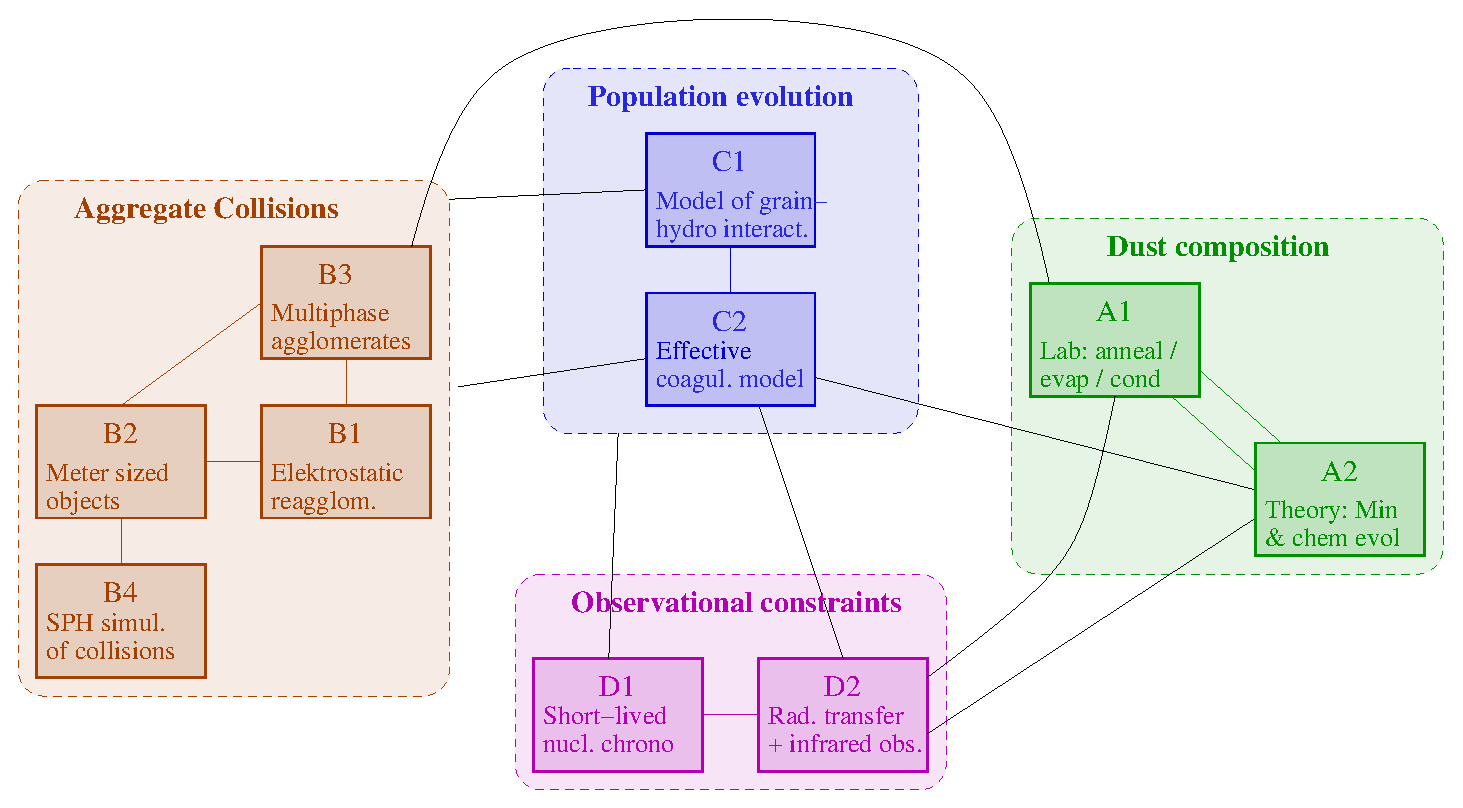
\includegraphics[width=16cm]{diagram.eps}}
%\vspace{1em}
%Fig 1: A diagram showing the links between the various
%projects. See text for details.\\
%
\centerline{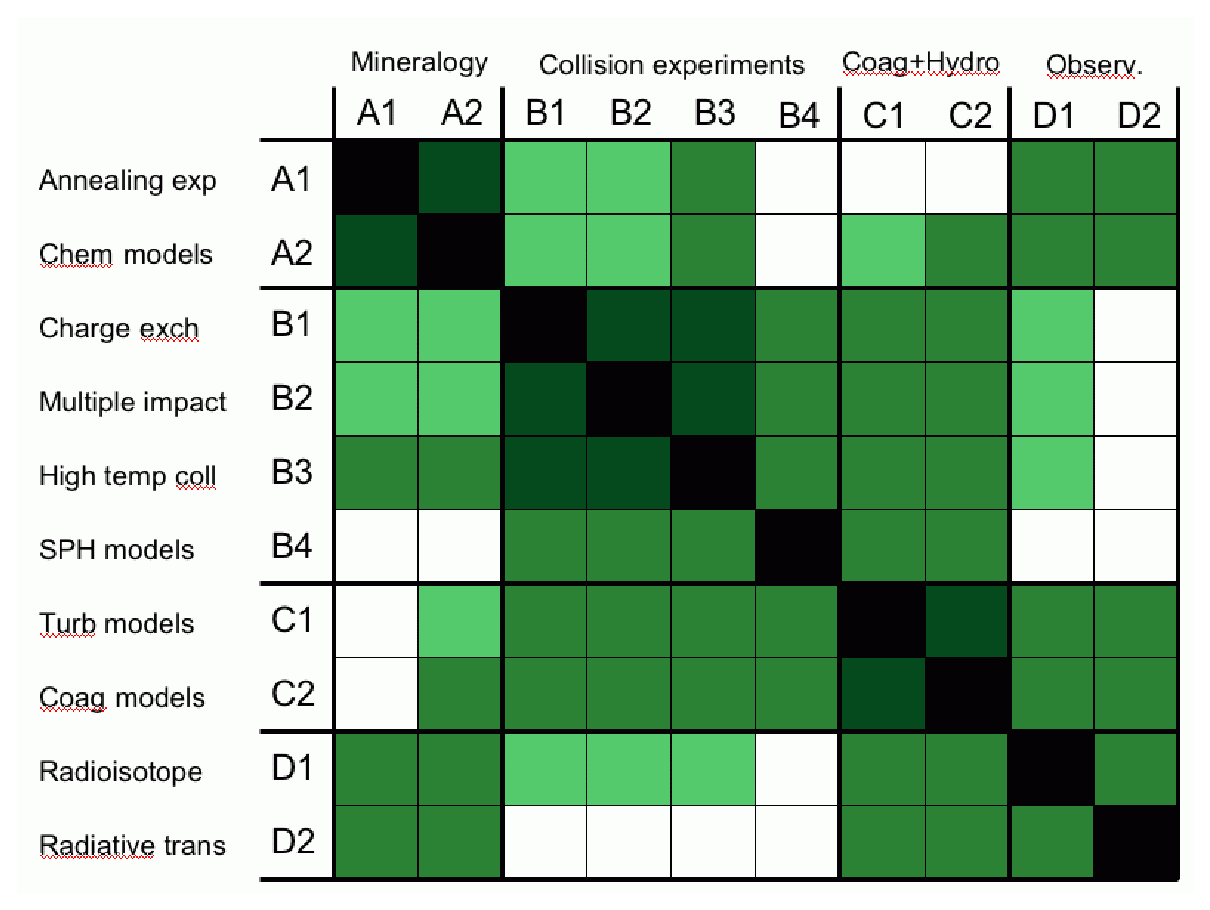
\includegraphics[width=12cm]{crosstable.eps}}
\vspace{1em}
Fig 1: A diagram showing the links between the various
projects. Dark-green means intense collaboration, on a
daily/weekly basis (5 links); intermediate green
means direct collaboration by exchange of data and iteration
between projects (23 links); light green means 
moderate collaboration, exchange of ideas (8 links). 
See text for details.\\
\vspace{2em}\mbox{}\\
\centerline{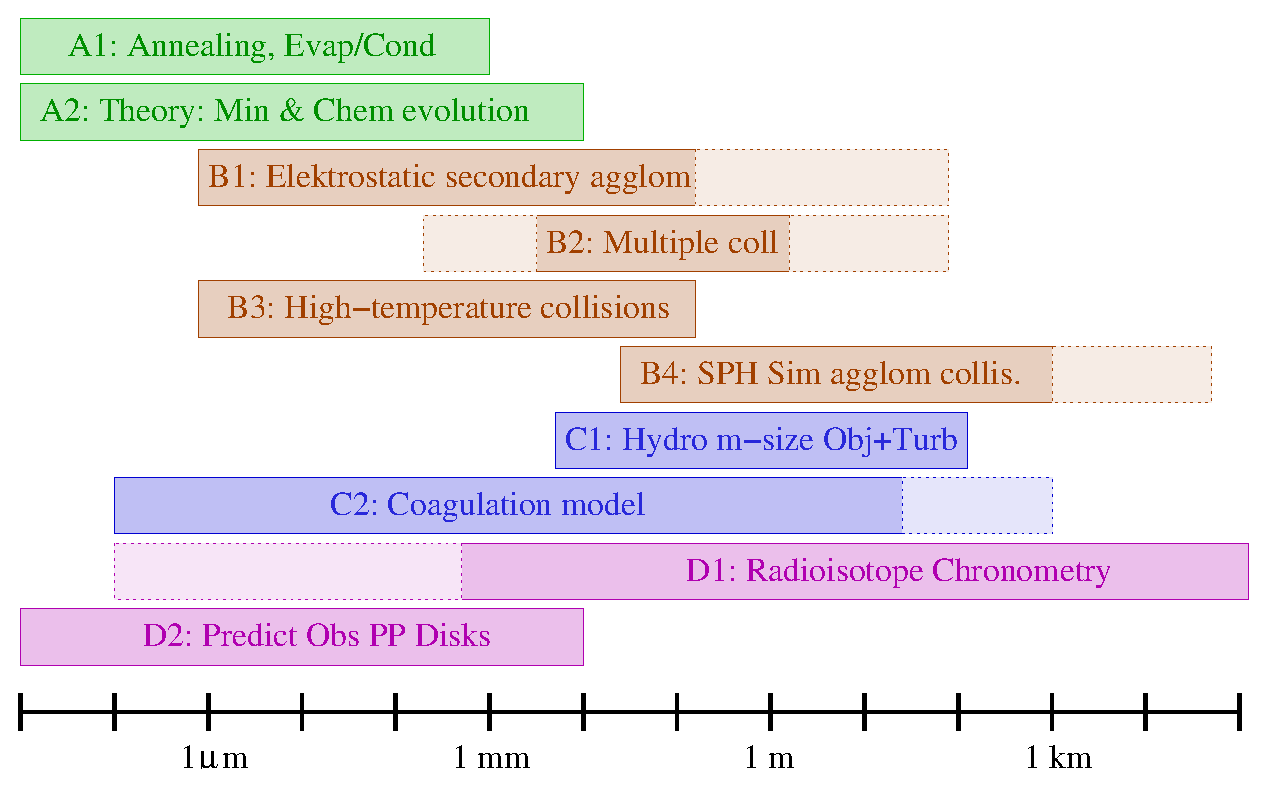
\includegraphics[width=16cm]{sizebar.eps}}
\vspace{1em}\\
Fig 2: A diagram showing the coverage
of the size-range between sub-micron dust particles and
multi-kilometer-sized planetesimals.
\end{figure}

\vspace{1.0em}

%
% Table with cross-connections
%
%\textbf{[***CHECK QUESTION MARKS BELOW***]}

% \newcommand{\chk}{$\surd$}
% \newcommand{\chkk}{$\surd\surd$}
% \begin{tabular}{l||cc|cccc|cc|cc}
%     &  A1  &  A2  &  B1  &  B2  &  B3  &  B4  &  C1  &  C2  &  D1  &  D2  \\
% \hline
% \hline
% A1  &      &\chkk &  .   &  .   & \chk &      &      &      & \chk & \chk \\
% A2  &\chkk &      &      &      & \chk &      &  ??  & \chk & \chk & \chk \\
% \hline
% B1  & \chk & \chk &      &\chkk &      & \chk & \chk &\chkk ?&     &      \\
% B2  &      &      &\chkk &      &      & \chk & \chk & \chk &      &      \\
% B3  & \chk & \chk &\chkk &\chkk &      & \chk & \chk & \chk &      &      \\
% B4  &      &      & \chk & \chk & \chk &      & \chk & \chk &      & \chk ?\\
% \hline
% C1  &      & \chk & \chk & \chk & \chk & \chk &      & \chk & \chk & \chk ?\\
% C2  &      & \chk & \chk & \chk & \chk & \chk &      &      & \chk & \chk \\
% \hline
% D1  &      & \chk & .?   & .?   & .?   & .?   & \chk & \chk &      & \chk \\
% D2  & \chk & \chk &      & \chk &      &      & \chk & \chk & \chk &      \\
% \hline
% \end{tabular}

\pagebreak[4]

\subsection*{\em Description of Scientific Blocks}
\vspace{0.5em}
In the following we present an overview of the contents of the four major
blocks in our Forschergruppe.
\vspace{0.8em}
 
\noindent\underline{{\bf Block \blockmineral{}:} Dust composition \& chemistry}
\vspace{0.8em}\\
%
%
The study of the composition and chemistry of solid material in
protoplanetary disks is required for the interpretation of infrared
observations of protoplanetary disks. 
% Without knowledge of dust composition
% and chemistry -- obtained from theoretical modeling and laboratory
% experiments -- it is difficult to extract information about the physical and
% chemical processes affecting the dust grains from the observed solid state
% features in the spectra of these protoplanetary disks.  
Such knowledge is also required for understanding the composition of comets,
asteroids, planets, including their atmospheres, oceans, and complex organic
materials.

In projects \projlattard{} and \projtscharn{} it is planned to investigate
the basic mineralogical and chemical processes that determine the properties
and the constituents of the dust mixture in protoplanetary disks. It will be
done for the first time in a consistent way by a joint interdisciplinary
effort of mineralogical laboratory investigations and astrophysical model
calculations.

The laboratory investigations in project \projlattard{} will analyze the
processes determining the composition and properties of the important
mineral components in the dust mixture. Presently, the most urgently needed
data for model calculations are realistic annealing data for interstellar
dust materials and vaporization/conden\-sa\-tion data for the dust materials
formed in the warm inner regions of accretion disks. Laboratory studies of
different groups have supplied already some data on silicate materials
(reviewed in Gail \cit{2003}) but important data are missing for
materials with the compositions expected to exist in protoplanetary disks.
In project \projlattard{} experiments will be performed on the
annealing and evaporation behavior of silicate compounds with varying
degrees of iron contents, which are expected to be the main dust
components. These experiments will provide the data required for realistic
models of the dust evolution in project \projtscharn{}. 
Vaporization and condensation experiments will be performed for the highly refractory
Calcium-Aluminum silicates for which hardly data are available yet.  These
experiments will be combined with an optical characterization of annealing
products and optical supervision of vaporization of thin films, which will
also supply optical data on important dust materials in temperature regions
not accessible to previous techniques, and they will provide necessary input data
for dust opacities, required in project \projwolf{}.

From the theoretical side we will (in project \projtscharn{}) approach this
problem by using a combination of modeling components. The structure and
evolution of the disk will be followed using time-dependent hydrodynamical models
coupled to a radiative transfer module. The chemistry of the solid and
gaseous components, as well as the physical and mineralogical processes
affecting the materials, will be modeled by extending previous work (Gail
\cit{2001, 2004}; Wehrstedt \& Gail \cit{2003}). Numerical tools for
calculating the structure and evolution of the disk with radiative transfer
(so far in the Eddington approximation, but extendible) are already
available, as well as subroutines for modeling transport processes and
chemical and mineralogical processes. Within the proposed project emphasis
is placed on the development of detailed chemical models for the chemical
evolution of the dust grains in the inner disk as well as on the formation
of ice coatings of grains in the outer disk regions. For both of these
aspects it is necessary to also model gas-phase chemistry in order to
predict the composition of the condensates.

The outcome of the models will provide important input-information required in
science block \blockimpact{} and project \projdul{} by specifying the
expected chemical composition of the colliding dust aggregates. Also it
predicts the abundances of certain minerals in protoplanetary disks, which are
required as input for radiative transfer modeling in project \projwolf{}.
The project needs input about general disk properties and evolutionary
timescales from projects \projtrie{} and \projwolf{}.
%

%\vspace{1em}\\

%\pagebreak[4]

%\noindent\underline{{\bf Block \blockimpact{}:} Collisions between dust
%aggregates}\\
%\mbox{}\vspace{1em}\\
\noindent\underline{{\bf Block \blockimpact{}:} Aggregate collisions}\\
%
The growth of dust from micrometer-sized particles to km-sized planetesimals
is a process involving a large sequence of individual collisions between
pairs of dust agglomerates. Whether such collisions lead to coalescence or
fragmentation depends on many parameters including the impact velocity and
the structure and composition of the aggregates involved. Laboratory
experiments have, over the past couple of years, yielded considerable
insight in the outcomes of such collisions, but large uncertainties
remain. These uncertainties include in particular collisions between bodies
exceeding a few cm in size and collisions between bodies of very different
sizes. In order to understand whether (and how) bodies can grow beyond the
`meter size barrier' the regime of high impact velocities and/or large
bodies must be studied in the laboratory and by using numerical
simulations. Two projects of block B intend to study the collisions of
aggregates in these new size regimes. The other two projects aim to study
additional effects of charge, temperature and composition on particle
growth. The laboratory experiments will be based on the huge progress in
experimental techniques of handling large monolithic dust samples and of
generating collisions between individual dust particles.
% 
% This will extensively broaden our knowledge of the outcomes of such
% collisions, with relevance to the formation stage of planetesimals.
%

In project \projblum{} we will study the role of charge separation during
collisions between small and large bodies on the growth process. A
succession of non-sticking collisions can lead to the build-up of strong
electric fields on the larger bodies from which emerging, previously
non-sticking dust particles are not able to escape. This project aims at the
experimental test of this concept and the modeling of the charge-induced
growth of planetesimals.

In project \projwurm{} laboratory experiments will be carried out with large
($>$ dm-sized) dust agglomerates subject to multiple collisions. It will be
studied if and how such agglomerates compactify, whether collisions lead to
growth or fragmentation, and whether debris products can re-accrete onto the
main body by hydrodynamic friction. The role of elastic waves and porosity
will be studied.

% The role of compaction, dilution, fragmentation, elastic waves, ejection 
% and re-accretion of material will be studied. 

In project B3 the collision experiments shall be extended to mineral phases
(Mg, Ca, Al silicates) that are expected from theoretical and observational
-- both astrophysical and cosmochemical -- constraints in protoplanetary
disks.  Particularly effects at high temperatures and dust/gas ratios
(sintering, eutectic melting between immiscible phases) could be key
mechanisms to trigger agglomerate growth beyond previously established
critical sizes (dm/m) and collision velocities (few m/s).

Parallel to the laboratory collision experiments, we will
(in project \projkley{}) perform numerical
simulations to determine the outcome of individual collisions between
aggregates. For this purpose an existing {\em Smooth Particle Hydrodynamics}
code for modelling elasto-plastic media will be adapted and 
calibrated with the laboratory data. With this code,
extrapolations on the collisional growth of dust aggregates to much larger
sizes will be possible and will allow the development of a realistic model
of planetesimal formation.

The embedding of these projects within the proposed Forschergruppe, in
particular the connection with science blocks \blockmineral{} and
\blockglobal{}, is of fundamental importance. First of all, the use of
realistic silicate dust mixtures in project B3 (and in the course of the
projects also B1 and B2) is a direct combination of collision experiments
and mineralogy. It is investigated how complex mineralogical compositions of
aggregates influence the outcome of collisions. Second, all projects of
block \blockimpact{} connect directly to block \blockglobal{}. The main
input parameters for the collision experiments, such as aggregate type, size
(project \projdul{}), and impact velocity (project \projklahr{}), can only
be determined in close collaboration with the models of block \blockglobal{}.
% It only makes sense to model
% collisions between certain aggregates with certain impact velocities if such
% aggregates indeed exist under these conditions, and if they indeed collide
% with these velocities. 
Moreover, the results of block \blockimpact{} have their highest relevance
when they can be applied to  models that can simulate the dust evolution on
a global scale (block \blockglobal{}), to study the effect of the lab
findings on the global particle population.
%
% using statistical methods (project \projdul{}), and models
% that can follow the transport of roughly meter-sized bodies through the disk
% (project \projklahr{}). This post-experiment modeling can tell what the
% effects of the laboratory findings are on the evolution of the particle
% distribution.
%
% For instance: knowing from block \blockimpact{} that certain
% collisions are destructive raises the question whether, as a consequence of
% this, most bodies of that size regime indeed suffer at least one such
% destructive collision, and whether the dust population is thereby
% significantly affected -- a question that can only be answered with the
% projects of block \blockglobal{}.  Vice versa, important input from Block
% \blockglobal{} about collision velocities is required for the projects in
% Block \blockimpact{}.
%

%\pagebreak[4]

%
\mbox{}\vspace{1em}\\
\noindent\underline{{\bf Block \blockglobal{}:} Particle population evolution}\\
%
%
%
\noindent The growth from dust to planetesimals is a process involving
extremely large numbers of particles. Each particle has its own location in
the protoplanetary disk and moves with its own velocity. While science block
\blockimpact{} is concerned with collisions between individual particles,
science block \blockglobal{} is concerned with the behavior of the dust {\em
population}. There are two main aspects: the systematic and random movements
of the particles through the disk and the evolution of the size-distribution
of the particles. In the Forschergruppe there will be a project to address
the first issue (project \projklahr{}) and a project to address the second
issue (project \projdul{}). 

In project \projklahr{} the movement of swarms of dust particles is modeled
with full magneto-hydrodynamics models.  This allows us to determine the
random and systematic motion of particles of different sizes, and thus
determine how often particles collide, and with which velocities. This is a
{\em fundamental} input parameter to dust coagulation models, and will be of
crucial importance to all the projects of block \blockimpact{}, as well as
to project \projdul{}. Additionally, it will be studied in this project
whether turbulence and vortices can concentrate the dust particles in small
regions which enhance the probability that they collide. With project
\projwolf{} it will be investigated if such concentrations can be observed in 
millimeter observations in the outer regions of protoplanetary disks.

In project \projdul{} we will develop a global coagulation model which solves
the evolution of the dust grain size distribution as a function of time and
location in the disk. This project is aimed at unifying the results of the
Forschergruppe into a single model, albeit with many simplifications to keep
the problem tractable. Outcomes from the various projects of the
Forschergruppe will be parameterized, tabulated or approximated by fitting
formulae, so that they can be incorporated into the model of project
\projdul{}, and the interconnection between all these processes be
investigated. This `effective model' will allow us to see what the effect of
all the microphysics from block \blockimpact{} and the mineralogy from block
\blockmineral{} is on the evolution of the particle population in
general. This can subsequently be channeled into the radiative transfer
modeling of project \projwolf{} to make observational predictions and allow
direct comparison to the observations.

%\pagebreak[4]


\mbox{}\vspace{1em}\\
\noindent\underline{{\bf Block \blockobserv{}:} Observational constraints}\\
%
\noindent Science block D has the aim of developing the interface between
the Forschergruppe and two main scientific fields that empirically constrain
the formation and growth of planetesimals. This will be in the form of
comparison to infrared/sub-millimeter observations of protoplanetary disks
and in the form of comparison to meteoritic data.

Infrared observations of protoplanetary disks yield data about if/where in
the disk certain dust mineralogical species at certain grain sizes reside.
The coagulation models (project \projdul{}), with input physics from
the collision experiments (block \blockimpact{}), yield predictions on the
expected life time of small dust grains in the disk and their average sizes.
The mineralogical/chemical models of project \projtscharn{} will predict the
thermal processing history of the dust and the radial mixing of these
various dust species. These models will yield the 2D and 3D grain
size/property distribution as a function of time, which can
directly be inserted in a radiative transfer code (project \projwolf{}) to
produce predictions for the spectral energy distributions {\em and} the
solid-state spectral features of these spectra.

While infrared observations give important information about growth
processes from micrometer to millimeter scales, another important
observational constraint on planetesimal formation is the timing of growth
from millimeter to 100 km size objects. For our own Solar System dating of
meteorite constituents can provide details with the time resolution of
better than a few hundred thousand years, by using long and short-lived
nuclide chronometry (Lugmair \& Shukolyukov \cit{1998}; Brazzle et
al.~\cit{1999}; Bizzarro et al.~\cit{2004}; Russell et~al.~\cit{1996}; Kita
et~al.~\cit{2000}; Trieloff et al.~\cit{2003}; Trieloff \& Palme
\cit{2006}).

In the case of the infrared observations (project \projwolf{}) the MPIA
already has the data-reduction and first-order interpretation of these data
as one of its main scientific activities. The (project \projwolf{}) aims to
connect the main activity of the Forschergruppe and the results from the
infrared observers at MPIA and in general. Additional help with this
interpretation will be given by other members of the Forschergruppe with
experience in comparing complex models to observations. In the case of
comparison to meteoritic data it must be kept in mind that this field is
already quite mature, and an enormous volume of knowledge is already
present. Comparison to this data can be done by the students from other
projects in close collaboration with the mineralogists of the
Forschergruppe. The proposed project on nuclide chronometry deals with the
key question of the timing of chondrule and planetesimal formation (Trieloff
\& Palme \cit{2006}), i.e. if chondrule formation is closely associated in
time and space to parent body formation with each parent body forming fast
(within a few 100\,000 years) from a restricted zone, or if chondrule
forming processes and subsequent incorporation into planetesimals allows
time for radial mixing of chondrules between different zones of the early
solar nebula.  
%
In another part of project D1, laboratory analysis of cometary dust samples
returned by the STARDUST mission will aim at quantifying the fraction of
material that experienced high temperature annealing, metamorphism,
condensation or evaporation and was transported outwards by radial mixing
processes into comet forming regions.


%% \mbox{}\vspace{1em}\\

\subsection*{\em Milestones}
\vspace{0.5em}
%
%%\mbox{}\vspace{1em}\\
%%\noindent{\bf \em Milestones}\vspace{0.8em}\\
%
\noindent The first 1.5 years will be a start-up phase: laboratory experiments will
be set up, numerical codes designed and first results booked (see below). During
this period, the collaboration between (and within) the individual projects is aimed
primarily at a transfer of know-how and expertise. After about 1.5 years, when
first results are expected, the focus of collaboration will gradually shift
to the exchange of results (i.e.~the results of one project being the input
to another). The main scientific objectives will then be targeted.

{\em Milestones block A:} In the startup phase we wish to obtain lab results
on Fe-bearing silicates, and first data on Ca,Al compounds. A first version
of disk models with gas phase and solid state chemistry will be developed.
In the second phase lab results from \projlattard{} will be used in
\projtscharn{}, model predictions on the location of crystalline silicates in
disks will be exported to \projwolf{}. Subroutines for solid state chemistry
and coagulation will be exchanged with \projdul{}. We expect to be able to
answer whether radial mixing theories can explain the variable composition
of volatile and refractory elements in our own Solar System and the
observational data on crystalline silicates in protoplanetary disks. 

% The
% issue to explain oxygen isotopic compositions of chondrites is certainly
% more challenging, and may be addressed in a possible extension of the
% Forschergruppe.

{\em Milestones block B:} In the initial phase existing experimental setups
will be modified, e.g.~implementing charge-transfer measurement equipment
for \projblum{} and preparation of multi-phase agglomerates for
\projblumtrie{}. The main measuring phase can already start after about 9
months. First data (e.g.~growth/erosion rates of charged impacts
(\projblum{}) / porous objects (\projwurm{}), sticking coefficients of
multi-phase agglomerates (\projblumtrie{})) will be transferred to other
blocks after about 1.5 years, and refined in the following years. The
numerical modeling of project \projkley{} will start with the implementation
of a more detailed porosity model in the existing SPH code,
and comparison and validation against
the lab experiments of block \blockimpact{}. In the second half of the
project a survey will be conducted of two-body aggregate collisions of
sizes larger than reachable in the laboratory. These data will then be
transmitted to other projects after about 2 years. 


{\em Milestones block C:} Due to the challenging nature of the hydrodynamic
simulations of project \projklahr{}, the first 1.5 years will be spent
mainly on the development and testing of the numerical tools such as radiative
transport in the diffusion approximation. First
realistic estimates of collision velocities and rates, as well as transport
of particles are expected by this time, and transmitted to science block
\blockimpact{} over the next 1.5 years. For project \projdul{} we will first
develop recipes for implementing experimental results into the coagulation
code. This will involve an extra `dimension' (dust property). At first we
will use already available lab data, and by about 1.5 years the new data
from the Forschergruppe will be implemented. The focus will then shift to
the application of the models to solving the outstanding scientific
questions mentioned in the project description.


{\em Milestones block D:} Project \projtrie{}: In the startup phase we aim
to obtain first chronological results (I-Xe, Al-Mg) on a first series of
chondrules from ordinary and carbonaceous chondrites. The most promising
meteorites will be selected in the second phase, in order to check the
relative timing of chondrule and chondrite formation. We expect constraints
on possible radial mixing processes of chondrules in the disk, and hints at
possible processes that speed up or delay planetesimal formation. 
%
From Stardust analysis the preliminary examination phase should allow a
rough estimate of the fraction of high temperature material found in comets.
%
Project \projwolf{}: In the first half existing models of
circumstellar disks will be used to study the influence of various disk and
dust parameters on observable quantities. As the project proceeds, new
results from the Forschergruppe will be considered and the disk models
improved accordingly. By this time the dust production by collisions of
planetesimals will be added to the models.



% Examples of such output-input exchange are:
% using collision velocity predictions from hydrodynamic simulations in lab
% experiments, taking into account the results from lab collision experiments
% and theory in coagulation models, using new lab data of thermal processing
% of minerals in theoretical models, using refined models of dust evolution
% and transport in disks for radiative transfer models for infrared spectra.

\subsection*{\em Future perspectives}
%%\mbox{}\vspace{1em}\\
%%\noindent{\bf \em Future perspectives}\vspace{0.8em}\\
%
This Forschergruppe proposal is focused entirely on the initial growth phase
of planets. 
Even though we hope to make good progress within the coming 3 years 
there will be probably more than enough open points and refinements for a
continuation of this work in the following funding period.
Additionally, we may envision to extend the focus and 
include studies of gravitational clustering of planetesimals, the capturing
of gas by protoplanets and the eventual formation of rocky and gas giant
planets. 
By that time major new developments are expected in the field of
observations of extrasolar planets which can constrain our models.


\section{Preconditions of the Forschergruppe}
\subsection*{\em In-house activities on meteoritics and observational astronomy}
%
%%\mbox{}\vspace{1em}\\
%%\noindent{\bf \em In-house activities on meteoritics and observational
%%astronomy}\vspace{0.8em}\\
%
Science block D has the aim of developing the interface between the
Forschergruppe and two main scientific fields that empirically constrain the
formation and growth of planetesimals. These fields are already strongly
represented by our current research:
%
\begin{itemize}
%
\item {\bf Composition of meteorites}\\
%
The wealth of data available from meteoritic and planetary science,
including aspects of mineralogy, isotope chronology, cosmochemistry and
geology needs to be incorporated into astrophysical models. Specific studies
related to the early evolution of meteorite parent bodies (M.~Trieloff), as
well as general experience in analytical and experimental mineralogy and
petrology (D.~Lattard, R.~Altherr) will guarantee the transfer of
geoscientific aspects into the interdisciplinary projects of the
Forschergruppe.

\item {\bf Observations of protoplanetary disks:}\\
%
In spite of the enormous surge in observational data of protoplanetary disks
currently arriving from e.g.~the Spitzer Space Telescope, the Very Large
Telescope and other facilities, our Forschergruppe does not require
personnel for the acquisition, reduction and first analysis of these
data. The MPIA has a large team of scientists dedicated to this task, and
the involvement of the MPIA in the Forschergruppe guarantees access to large
quantities of reduced and directly useable data. 
%Some members of the
%Forschergruppe (S.~Wolf, Th.~Henning and C.P.~Dullemond) have strong
%connections to the observational community both inside the MPIA and outside.
\end{itemize}

%
% 
\subsection*{\em Past and current activities}
The planned activities of the proposed Forschergruppe are part of an
increased scientific interest in the area of planet formation in Germany.

For several years now the contacts between the geophysical/mineralogical and
astrophysical scientific communities in Germany have intensified, mainly
through the organization of a series of ``Planet Formation'' workshops,
specifically meant to create a platform for discussion and interaction
across fields.  These were held over the past 5 years in Berlin, Weimar,
M\"unster and most recently in Heidelberg (this March).  The last two
meetings of this series have been organized by members of the proposed
Forschergruppe: G.~Wurm (PI of project B2), S.~Wolf (PI of project D2) and
M.~Trieloff (Co-Speaker of this Forschergruppe), and the next workshop is
planned to take place in 2007 in Braunschweig (organized by J.~Blum, PI of
projects B1 and B3).

At the same time the Max-Planck-Institute for Astronomy in Heidelberg has
organized several international workshops on very closely related
fields. The latest one was on Planet Formation in Ringberg, December 2004,
organized by H.~Klahr (PI of project C1) and W.~Brandner, from which a book
will soon published by Cambridge University Press. The next meeting,
organized by C.P.~Dullemond (Co-Speaker of this Forschergruppe) together
with H.~Klahr (PI project C1), has a topic very close to that of the
Forschergruppe: ``From Dust to Planetesimals'' and will be held in the very
near future (September 11-15, 2006) at Schlo{\ss} Ringberg.

In October 2005, S.~Wolf (PI of project D2) has organized a Heraeus School in
the field of Planet Formation, where many of the members of the FG have
given review talks about the status of the field and their own work related
to planet formation.

This short overview over activities in the field of Planet Formation in
Germany demonstrates clearly that {\it i)} interaction between the involved
scientists has taken place already, and that {\it ii)} there is rising
interest to combine efforts, and team-up to resolve scientific problems in close
collaboration.

\section{Education, communication and logistics of the Forschergruppe}
%
The sub-projects proposed in this Forschergruppen-proposal will be carried out
exclusively by PhD students under the supervision of the PIs of the
sub-projects. The topic of planetesimal formation is a modern, flourishing
and multi-disciplinary field of science in which the PIs of our proposed
Forschergruppe can -- and will -- provide an excellent and stimulating
working environment for the PhD students.

We propose 10 projects, with (in total) 13 PhD positions. Of those 13
positions, 11 are planned to be financed by the DFG (through the
Forschergruppe) while 2 PhD positions will be financed by the participating
institutes.

One of the pillars of our proposed Forschergruppe is the collaboration and
communication between the various teams. Some PhD students will have
advisors at different institutions and even at different locations. In other
cases the main work is done in one institute, but strong interaction is
required with the other institutions. For this reason we intend to include a
relatively large travel budget in our proposal. Each PhD student should have
the possibility to spend three weeks per year on a work visit in one of the
other nodes or up to three weeks in total spread over multiple work visits
to various nodes. For some of the PhD students, in particular those which
are shared by two institutes, longer work visits should be possible.

Regular small informal meetings will be organized between a subset of the
groups. Travel possibilities should be available for regular spontaneous
one- or two-day meetings of about 4 to 6 persons: e.g.~two collaborating PhD
students and their respective advisors.

%In addition to this we intend to invite international guests for one- or
%two-week visits to one--but preferably more--of the institutes of the
%Forschergruppe.

We intend to set up a bi-weekly Forschergruppe-Seminar, using
video-confe\-rencing methods. In each of these seminars, one of the PhD
students will report his/her latest developments, and in the rest of the
time there will be room for general discussion.

Twice a year a full group meeting of 3 days will be organized, starting
from the beginning of the second year.   These
meetings will be organized in a quiet isolated environment and will be half
in the form of talks and half entirely informal, providing sufficient time
for discussions.  During these meetings it will be possible to improve
connections and to focus on the target issues of the Forschergruppe. We
intend to invite one or two internationally acclaimed guests to these
meetings to give guest lectures on topics of common interest within the
Forschergruppe. The visit of these guests can/will be extended with a 1 week
visit to one or more of the nodes.

After the first half year, roughly summer 2007, a summer school will be
organized which covers all the topics of the Forschergruppe. This is
essential in order to guarantee that each student has a good enough level of
knowledge of the relatively broad interdisciplinary field covered by the
Forschergruppe, such that the planned interactions between the projects will be
successful. Although the primary focus will clearly be on the PhD students
of the Forschergruppe, the school will be open to all astronomy PhD students
from Germany and abroad. We will also invite international lecturers 
with an outstanding reputation.

\section{Forschergruppen-Professur}
%
One of the major goals of the proposed Forschergruppe is the initiation of
a close collaboration of researchers from different scientific communities
to jointly study the formation of planets around solar type stars.
At the heart of this effort lies the combination of geological/mineralogical
research with astronomy and astrophysics.  
This aim of our research group can be realized best through the creation of
a new Forschergruppen-Professur in the area of 
``Geoscientific and Astrophysical Planetary Research''. 
Heidelberg, where the main part of this Forschergruppe is localized,
constitutes the ideal location to create such a professorship.
The University of Heidelberg has prepared plans on how to announce and fill such
a professorship.
A more detailed justification of the requested position is given in project P. 
%

\newpage
\renewcommand{\hdrtitle}{Financial Overview}
\section{Financial Overview}
The total funds requested in all categories for all 10 projects are
summarized in the following tables (all amounts in \EUR).
%

\medskip

\subsection*{Personnel}
In all scientific projects the requested positions refer to
PhD students, where we ask for funding for 11 positions. 
The salary level refers to E13/2 (formerly Bat IIa/2). 
Two further PhD
positions (in projects A2 and C1) are funded by the ITA and the MPIA. 
These are denoted by (1/2) in table below.

\noindent
In project A1 and D1 additional funds are requested for
student research assistants (HiWis) for two
years to support the experimental work.
\\[0.2cm]
%
\centerline{\begin{tabular}{||l|r|r|r||}
\hline \hline 
 Project  & Year 1 & Year 2 & Year 3 \\ \hline %
 A1       & 56.500  & 56.500  & 48.000  \\
 A2 (1/2) & 24.000  & 24.000  & 24.000  \\
 B1       & 24.000  & 24.000  & 24.000  \\
 B2       & 24.000  & 24.000  & 24.000  \\
 B3       & 24.000  & 24.000  & 24.000  \\
 B4       & 24.000  & 24.000  & 24.000  \\
 C1 (1/2) & 24.000  & 24.000  & 24.000  \\
 C2       & 24.000  & 24.000  & 24.000  \\
 D1       & 28.500  & 26.250  & 24.000  \\
 D2       & 24.000  & 24.000  & 24.000  \\
\hline
{\bf Total:} (EUR)       & 277.000  & 274.750 & 264.000 \\
\hline \hline
\end{tabular}
}

\vspace{2.0cm}

%
\subsection*{Consumables}
The amounts for consumables refer primarily to materials that
have to used in the experimental studies.
\\[0.2cm]
% 
\centerline{\begin{tabular}{||l|r|r|r||}
\hline \hline
 Project  & Year 1 & Year 2 & Year 3 \\ \hline %
 A1       & 16.250  & 16.250  & 10.000  \\
 A2       &    400  &    400  &    400  \\
 B1       &  9.000  &  7.000  &  6.000  \\
 B2       &  1.240  &  1.240  &  1.240  \\
 B3       &  8.408  &  8.000  &  7.000  \\
 B4       &   -     &   -     &   -     \\
 C1       &   -     &   -     &   -     \\
 C2       &   -     &   -     &   -     \\
 D1       &  8.300  &  8.300  &  4.800  \\
 D2       &   -     &   -     &   -     \\
\hline
{\bf Total:} (EUR)       &  43.598    & 41.190   &  29.440 \\
\hline \hline
\end{tabular}
}

\newpage
%
\subsection*{Travel}
The amounts for travel refers to money allocated directly to the
individual projects, first to support longer term visits between the
different closely collaborating nodes of the Forschergruppe, and second
expenditures related to experimental studies that have to
be conducted outside of the Forschergruppe. This money is in addition to
that in project Z.
\\[0.2cm]
% 
\centerline{\begin{tabular}{||l|r|r|r||}
\hline \hline 
 Project  & Year 1 & Year 2 & Year 3 \\ \hline %
 A1       &  4.046  &  4.046  &  1.368  \\
 A2       &  3.000  &  3.000  &  3.000  \\
 B1       &  4.000  &  5.600  &  5.600  \\
 B2       &  3.810  &  3.810  &  3.810  \\
 B3       &  5.100  &  6.700  &  6.700  \\
 B4       &  2.760  &  2.500  &    570  \\
 C1       &  2.820  &  2.820  &  2.820  \\
 C2       &  4.640  &  2.720  &  2.540  \\
 D1       &  6.129  &  6.129  &  1.356  \\
 D2       &  1.300  &  1.300  &  1.300  \\
\hline
{\bf Total:} (EUR) &   37.605   &   38.625 &    29.064  \\
\hline \hline
\end{tabular}
}

\vspace{2.0cm}

%
\subsection*{Small Equipment}
Investments necessary for carrying out the experiments.
\\[0.2cm]
%
\centerline{\begin{tabular}{||l|r|r|r||}
\hline \hline 
 Project  & Year 1 & Year 2 & Year 3 \\ \hline %
 A1       & 27.000  &   -     &   -     \\
 A2       &   -     &   -     &   -     \\
 B1       & 12.269  &   -     &   -     \\
 B2       &   -     &   -     &   -     \\
 B3       & 16.771  &  2.500  &   -     \\
 B4       &   -     &   -     &   -     \\
 C1       &   -     &   -     &   -     \\
 C2       &   -     &   -     &   -     \\
 D1       &   -     &   -     &   -     \\
 D2       &   -     &   -     &   -     \\
\hline
{\bf Total:} (EUR)       & 56.040  & 2.500 & - \\
\hline \hline
\end{tabular}
}

\newpage

%
\subsection*{Others costs}
Materials for experimental work and 
computer equipment in more theoretical studies.
\\[0.2cm]
%%
\centerline{\begin{tabular}{||l|r|r|r||}
\hline \hline
 Project  & Year 1 & Year 2 & Year 3 \\ \hline %
 A1       &  9.250  &  9.250  &  7.250  \\
 A2       &   -     &   -     &   -     \\
 B1       &   -     &   -     &   -     \\
 B2       &  1.000  &         &         \\
 B3       &   -     &   -     &   -     \\
 B4       &  2.000  &   -     &   -     \\
 C1       &  4.000  &   -     &   -     \\
 C2       &  2.000  &   -     &   -     \\
 D1       &  3.200  &  3.200  &   -     \\
 D2       &  2.000  &   -     &   -     \\
\hline
{\bf Total:} (EUR)       &   23.450    &  12.450    &   7.250    \\
\hline \hline
\end{tabular}
}

\medskip

%
\subsection*{Central Budget}
The total funds requested for Project Z are summarized in the following table.
\\[0.2cm]
\centerline{\begin{tabular}{||l|r|r|r||}
\hline \hline & Year 1 & Year 2 & Year 3 \\ \hline %
Networking                  & 24.800  & 41,800  & 41,800  \\
External Travels            & 30.000  & 30.000  & 30.000  \\
External Guests             & 30.000  & 30.000  & 30.000  \\
Conference/Summerschool     & 20.000  &   -     & 20.000  \\
Consumables                 &  1.000  &  1.000  &  1.000  \\
Publications                &  5.000  &  5.000  &  5.000  \\
Management    (Bat Vb/2)    & 21.000  & 21.000  & 21.000  \\
\hline
{\bf Total:} (EUR)          & 131.800  & 128.800 & 148.800 \\
\hline \hline
\end{tabular}
}

\medskip

%
\subsection*{\large Total Budget}
Listing of total costs
\\[0.2cm]
%
\centerline{\begin{tabular}{||l|r|r|r||}
\hline \hline
 Item              & Year 1 & Year 2 & Year 3 \\ \hline %
 Positions (PhD/HiWi)  & 277.000  & 274.750 & 264.000 \\
 Travel (projects)     &  37.605  &  38.625 &  29.064  \\
 Small Equipment       &  56.040  &   2.500 &   -     \\
 Consumables           &  43.598  &  41.190 &  29.440 \\
 Other Costs           &  23.450  &  12.450 &   7.250  \\
 Project P             &  80.000  &  80.000 &  80.000 \\
 Project Z             & 131.800  & 128.800 & 148.800 \\
\hline \hline
{\bf Total:} (EUR)     & 649.493  & 578.315 & 558.554  \\
\hline \hline 
\end{tabular} 
}

\newpage
%
\renewcommand{\hdrtitle}{Signatures}
\section{Signatures}
%
The project leaders have agreed to be responsible for the scientific
work of their projects.\\[0.4cm]
%
\noindent
The Speaker and co-Speakers of the Forschergruppe:\\[0.4cm]
% 
\noindent
{\it The Formation of Planets: The Critical First Growth Phase}
\\[1.0cm]
%
% \noindent
% \begin{tabular}{p{5.5cm}p{5.5cm}p{5.5cm}}
% Prof.\ Wilhelm Kley    &  Dr.\ Cornelis~P. Dullemond   &  Dr.\ Mario~Trieloff \\
% Institut f\"ur Astronomie  &  Max-Planck-Institut      &  Mineralogisches Institut  \\
% \& Astrophysik         &  f\"ur Astronomie             &  Universit\"at Heidelberg \\
% Universit\"at T\"ubingen & 69117 Heidelberg            &  69120 Heidelberg \\
% 72076  T\"ubingen  & & \\
% \vspace{1em} & & \\
% %
% T\"ubingen, May 30, 2006 & Heidelberg, May 30, 2006 & Heidelberg, May 30, 2006\\
% \vspace{1em} & & \\
% %
% 
\epsfig{file=signature_kley.eps,width=50mm} & & \\
% \vspace{1em} & & \\
% Wilhelm Kley & Cornelis P. Dullemond & Mario Trieloff \\
% \end{tabular}
% 
\noindent
Prof.\ Wilhelm Kley\\
Institut f\"ur Astronomie \& Astrophysik\\
Universit\"at T\"ubingen\\
72076  T\"ubingen\vspace{1em}\\

\noindent Dr.\ Cornelis~P. Dullemond\\
Max-Planck-Institut f\"ur Astronomie\\
69117 Heidelberg\vspace{1em}\\

\noindent Dr.\ Mario~Trieloff\\
Mineralogisches Institut\\
Universit\"at Heidelberg\\
69120 Heidelberg\vspace{4em}\\

\noindent T\"ubingen, May 30, 2006\\[1em]

\noindent\begin{tabular}{p{5.5cm}p{5.5cm}p{5.5cm}}

\epsfig{file=signature_kley.eps,width=50mm} & 

\epsfig{file=signature_dul.eps,width=50mm} & 

\epsfig{file=signature_trie.eps,width=50mm}\\
\vspace{1em} & & \\
Wilhelm Kley & Cornelis P. Dullemond & Mario Trieloff \\
\end{tabular}
% 



% Prof. Wilhelm Kley  \\
% Institut f\"ur Astronomie \& Astrophysik \\
% Universit\"at T\"ubingen \\
% 72076  T\"ubingen
% \\[2.5cm]
% 
% 
% T\"ubingen, May 30, 2006 
% 
% \medskip
% 
% 
\epsfig{file=signature_kley.eps,width=50mm}\\Wilhelm Kley


%
\vfill 
$~$


\pagebreak[4]


\clearpage
\renewcommand{\hdrtitle}{References}

\clearpage

\section{References}
\begin{literature}
\item 
Ahrens, T.~J. and Rubin, A.~M. (1993) Impact-induced tensional failure in rock.
\textit{J. Geophysical Res.} \textbf{98}, 1185

\item 
Amelin, Y., Krot, A., Hutcheon, I.~D. and Ulyanov, A.~A. (2002)
Lead Isotopic Ages of Chondrules and Calcium-Aluminum-Rich Inclusions. 
\sci \textbf{297}, 1678

\item
Apai, D., Pascucci, I., Bouwman, J., Natta, A., Henning, Th. and
Dullemond, C.P. (2005) The onset of planet formation in Brown Dwarf disks.
\sci, \textbf{310}, 834

\item 
Balbus, S.~A. and Hawley, J.~F. (1998) Instability, turbulence and enhanced
transport in accretion disks, \rmf \textbf{70}, 1

\item 
Barge, P. and Sommeria, J. (1995) Did planet formation begin inside
persistent gaseous vortices?, \aap \textbf{295}, L1

\item 
Beckwith, S.~V.~W. and Sargent, A.~I. (1991) Particle emissivity in
circumstellar disks. \apj \textbf{381}, 250

\item 
Bell, K.~R., Cassen, P.~M., Klahr, H.~H. and Henning, Th. (1997) 
The Structure and Appearance of Protostellar Accretion Disks: 
Limits on Disk Flaring. \apj \textbf{486}, 372

\item 
Benz, W. (2000) Low Velocity Collisions and the Growth of Planetesimals.
\ssr \textbf{92}, 279

\item 
Benz, W. and Asphaug, E. (1994) Impact simulations with fracture. I - Method
and tests. \ica \textbf{107}, 98

\item 
Bizzarro, M., Baker, J.~A. and Haack, H. (2004) Mg isotope evidence for
contemporaneous formation of chondrules and refractory inclusions. \nat
\textbf{431}, 275

\item 
Blum, J., Wurm, G., Poppe, T. and Heim, L.-O. (1999) Aspects of Laboratory Dust
Aggregation with Relevance to the Formation of Planetesimals. In:
\textit{Laboratory Astrophysics and Space Research}, Astrophysics and Space
Science Library, Vol. \textbf{236} (Eds. P. Ehrenfreund, K. Krafft, H. Kochan,
V. Pirronello) Kluwer Academic Publishers, Dordrecht, 399

\item 
Blum, J. and Wurm, G. (2000) Experiments on Sticking, Restructuring and
Fragmentation of Preplanetary Dust Aggregates. \ica \textbf{143}, 138-146

\item 
Blum, J., Wurm, G., Kempf, S., Poppe, T., Klahr, H., et al. (2000) Growth
and Form of Planetary Seedlings: Results from a Microgravity Aggregation
Experiment.
\prl \textbf{85}, 2426-2429

\item 
Blum, J. (2004) Grain Growth and Coagulation. In: \textit{Astrophysics of
Dust}, ASP Conference Series, Vol. \textbf{309} (Eds. A. Witt, G. Clayton and
B. Draine), 369-391

\item 
Blum, J. and Schr\"apler, R. (2004) Structure and Mechanical Properties of
High-Porosity Macroscopic Agglomerates Formed by Random Ballistic Deposition.
\prl \textbf{93}, 115503

\item 
Bockel\'ee-Morvan, D., Gauthier, D., Hersant, F., Hur\'e J.-M. and Robert,
F.  (2002) Turbulent radial mixing in the solar nebula as the source of
crystalline silicates in comets. \aap \textbf{384}, 1107

\item 
Bouwman, J., de Koter, A., van den Ancker, M.~E. and Waters,
L.~B.~F.~M. (2000) The composition of the circumstellar dust around the
Herbig Ae stars AB Aur and HD 163296. \aap \textbf{360}, 213

\item 
Bouwman, J., Meeus, G., de Koter, A., Hony, S., Dominik, C. and Waters,
L.~B.~F.~M. (2001) Processing of silicate dust grains in Herbig Ae/Be
systems.
\aap \textbf{375}, 950

\item 
Brazzle, R.~H. (1999) Verification and interpretation of the I-Xe chronometer.
\gca \textbf{63}, 739

\item 
Bridges, F. G., Supulver K. D., Lin, D. N. C. {\it et al.}
(1996) Energy loss and sticking mechanisms in particle aggregation in
planetesimal formation. \ica \textbf{123}, 422

\item
Brownlee D. E., Burnett D. {\em et~al.} (1996).  Stardust: Comet and
interstellar dust sample return mission, in \textit{Physics, Chemistry,
and Dynamics of Interplanetary Dust}, ed. B.A.S.~Gustafson and
M.S.~Hanner (ASP Conf. Series 104).

\item 
Brucato, J.~R., Colangeli, L., Mennella, V., Palumbo, P. and Bussoletti, E.
(1999) Mid-infrared spectral evolution of thermally annealed amorphous
pyroxene. \aap \textbf{348}, 1012

\item 
Brucato, J.~R., Mennella, V., Colangeli, L., Rotundi, A. and Palumbo,
P. (2000) Production and processing of silicates in laboratory and in
space. \pss \textbf{50}, 829

\item 
Carpenter, J.~M., Wolf, S., Schreyer, K., Launhardt, R. and Henning,
Th. (2005) Evolution of Cold Circumstellar Dust around Solar-type Stars. \aj
\textbf{129}, 1049

\item 
Chokshi, A.,  Tielens A. G. G. M. and Hollenbach, D. (1993)
Dust coagulation \apj \textbf{407}, 806 

\item 
Clayton, R.~N. (1993) Oxygen isotopes in meteorites. \textit{Ann. Rev. Earth
\& Planetary Sci.} \textbf{21}, 115

\item 
Cuzzi, J.~N., Dobrovolskis, A.~R. and Champney, J.~M. (1993) 
Particle-gas dynamics in the midplane of a protoplanetary nebula
\ica \textbf{106}, 102

\item 
Cuzzi, J., Hogan, R. C., Paque, J. M., Dobrovolskis, A. R. (2001)
Size-selective concentration of chondrules and other small particles in
protoplanetary nebula turbulence \apj \textbf{546}, 496

\item 
Dahneke (1975)   J.~Colloid Interf.~Sci. \textbf{1}, 58 

\item D'Alessio, P., Calvet, N. and Woolum, D.S. (2005) Thermal structure of
  protoplanetary disks. In: \textit{Chondrites and the protoplanetary disk\/},
  ASP Conf. Ser. Vol. 341 (Eds. A.N. Krot, E.R.D. Scott, B. Reipurth), 353

\item 
Dominik, C. and Tielens, A.~G.~G.~M. (1997) The Physics of Dust Coagulation
and the Structure of Dust Aggregates in Space. \ica \textbf{480}, 647

\item 
Dullemond,~C.~P. (2002) The 2-D structure of dusty disks around Herbig Ae/Be
stars. I. Models with grey opacities. \aap \textbf{395}, 853

\item 
Dullemond, C.~P. and Natta, A. (2003) The effect of scattering on the
structure and SED of protoplanetary disks. \aap \textbf{408}, 161

\item 
Dullemond, C.~P. and Dominik, C. (2004) Dust settling in disks: from flaring
to self-shadowing. \aap \textbf{421}, 1075

\item 
Dullemond, C.~P. and Dominik, C. (2004) Flaring vs. self-shadowed disks: The
SEDs of Herbig Ae/Be stars. \aap \textbf{417}, 159

\item 
Dullemond C.~P. and Dominik, C. (2005) Dust coagulation in protoplanetary
disk: a too rapid depletion of small grains. \aap \textbf{434}, 971

\item {Dullemond}, C.~P. and {Apai}, D. and {Walch}, S. (2006)
  Crystalline Silicates as a Probe of Disk Formation History, 
  \apjl \textbf{640}, 67

\item Dullemond, C.P., Hollenbach, D., Kamp, I. \& D'Alessio, P. (2006)
  Models of the structure and evolution of protoplanetary disks, 
  in ``Protostars and Planets V'', eds. Reipurth, Jewitt \& Keil,\\ {\tt
  http://ifa.hawaii.edu/UHNAI/ppv.htm}

\item
Eisner, J.~A., Lane, B.~F., Akeson, R.~L., Hillenbrand, L.~A. and 
Sargent, A.~I. (2003) Near-Infrared Interferometric Measurements of 
Herbig Ae/Be Stars \apj \textbf{588}, 360

\item
Fabian, D., J\"ager, C., Henning, Th., Dorschner, J. and Mutschke, H. (2000)
Steps toward interstellar silicate mineralogy. V. Thermal Evolution of
Amorphous Magnesium Silicates and Silica. \aap \textbf{364}, 282

\item
Finocchi, F., Gail, H.-P. and Duschl, W.~J. (1997a) Chemical reactions in
protoplanetary disks II. Carbon dust oxidation. \aap \textbf{325}, 1264
 
\item
Finocchi, F. and Gail, H.-P. (1997b) Chemical reactions in protoplanetary
accretion disks III. The role of ionisation processes. \aap \textbf{327},
825

\item
Fischer, O., Henning, T. and Yorke, H.~W. (1996) Simulation of polarization
maps. II. The circumstellar environment of pre-main sequence objects.
\aap \textbf{308}, 863

\item
Forrest, W.~J., Sargent, B., Furlan, E., D'Alessio, P., Calvet, N.,
Hartmann, L., Uchida, K.~I., Green, J.~D., Watson, D.~M., Chen, C.~H. and 11
coauthors (2004) Mid-infrared Spectroscopy of Disks around Classical T Tauri
Stars.
\apjs \textbf{154}, 443

\item
Gail, H.-P. (2001) Radial mixing in protoplanetary accretion disks. I.
Stationary disc models with annealing and carbon combustion. \aap
\textbf{378}, 192-213

\item
Gail, H.-P. (2002) Radial mixing in protoplanetary accretion
disks. III. Carbon dust oxidation and abundance of hydrocarbons in
comets. \aap \textbf{390}, 253-265

\item
Gail, H.-P. (2003) Formation and Evolution of Minerals in Accretion Disks
and Stellar Outflows. In: \textit{Astromineralogy} (Ed. Th. Henning) Lecture
Notes in Physics Vol. \textbf{609}. Springer, Heidelberg. p. 55-120

%\item
%Gail, H.-P. (2003b) Radial mixing in protoplanetary accretion disks. IV.
%Metamorphosis of the silicate dust complex. \aap \textbf{413}, 571-591

\item
Gail, H.-P. (2004) Radial mixing in protoplanetary accretion disks. IV.
Metamorphosis of the silicate dust complex. \aap \textbf{413}, 571-591

\item
Gail, H.-P. and Tscharnuter, W.~M. (2005) Evolution of protoplanetary disks
including detailed chemistry and mineralogy. In: \textit{Reactive Flow,
Diffusion and Transport} (Ed. R. Rannacher et. al.) Springer,
Berlin-Heidelberg.  (accepted)

\item
Gilmour, J.~D., Pravdivtseva, O.~V., Busfield, A. and Hohenberg C.~M. (2004)
I-Xe and the chronology of the early solar system.  \textit{Workshop on
chondrites and the protoplanetary disk} abstr. no. 9054.

\item 
Gilmour J.D., Pravdivtseva O.V., Busfield A., and Hohenberg C.M. (2006).
The I-Xe chronometer and the early solar system.  
\textit{Met. Planet. Sci.} \textbf{41}, 19

\item
Gil, C., Malbet, F., Sch\"oller, M., Chesneau, O., Leinert, Ch. (2005)
Observations of 51 Ophiuchi with MIDI at the VLTI astro-ph/0508052

\item
Goldreich, P. and Ward, W.~R. (1973) The Formation of Planetesimals. \apj
\textbf{183}, 1051

\item
G\"unther, R., Sch\"afer, C. and Kley, W. (2004)  Evolution of irradiated
circumbinary disks \aap \textbf{423}, 559

\item
G\"unther, R. and Kley, W. (2002) Circumbinary disk evolution \aap
\textbf{387}, 550

\item
Haisch Jr., K.~E.,  Lada, E.~A. and Lada, C.~J. (2001) Disk Frequencies and
Lifetimes in Young Clusters. \apj \textbf{553}, L153

\item
Hallenbeck, S.~L.; Nuth, J.~A. and Daukantas, P.~L. (1998) Mid-Infrared
Spectral Evolution of Amorphous Magnesium Silicate Smokes Annealed in
Vacuum: Comparison to Cometary Spectra. \ica \textbf{131}, 198

\item
Harker, D.~E. and Desch, S.~J. (2002) Annealing of Silicate Dust by Nebular 
Shocks at 10 AU. \apj \textbf{565}, L109

\item Harker, D.E., Woodward, C.E., and Wooden, D.H. (2005) The dust grains
  from 9P/Tempel 1 before and after the encounter with deep
  impact. \textit{Science\/}, \textbf{310}, 278

\item
Hashimoto, A. (1990) Evaporation kinetics of forsterite and implications for
the early solar nebula. \nat \textbf{347}, 53

\item
Hashimoto, A. (1991) Evaporation of melilite. \textit{Meteoritics\/}
\textbf{26}, 344

\item
Hatzes, A. P., Bridges, F., Lin, D. N. C., Sachtjen, S. (1991)
Coagulation of particles in Saturn's rings - Measurements of the cohesive
force of water frost \ica \textbf{89}, 113

\item
Heim, L.-O., Blum, J., Preuss, M. and Butt, H.-J. (1999) Adhesion and
Friction Forces Between Spherical Micrometer-Sized Particles. \prl
\textbf{83}, 3328

\item
Henning, Th., Il'In, V. B., Krivova, N.A., Michel, B., Voshchinnikov, N.V.
(1999) WWW database of optical constants for astronomy \aaps \textbf{136},
405.

\item
Henning, Th. (2003) Astromineralogy Lecture Notes
in Physics Vol. \textbf{609}. Springer, Heidelberg.

\item
Hines, D. C., Backman, D. E., Bouwman, J. et al. (2006) 
Discovery of an unusual debris system associated with HD 12039 \apj,
\textbf{638}, 1070

\item
Honda, M., Kataza, H., Okamoto, Y.K., Miyata, T. et al. (2003) 
Detection of Crystalline Silicates around the T Tauri Star Hen 3-600A
\apj \textbf{585}, L59

\item
Hueso, R. and Guillot, T. (2003) Evolution of the Protosolar Nebula and
Formation of the Giant Planets. \ssr \textbf{106}, 105

\item
Ilgner, M., Henning, Th., Markwick, A.~J. and Millar, T.~J. (2004) Transport
processes and chemical evolution in steady accretion disk flows. \aap
\textbf{415}, 643

\item
Jessberger, E.K., A. Christoforidis, J. Kissel (1988): 
Aspects of the major element composition of Halley's dust.
Nature \textbf{332}, 691

Jessberger E.K. (1999) 
On the elemental, isotopic and mineralogical ingredients of
ROCKY cometary particulates.
Space Science Reviews \textbf{90}, 91

\item
Johansen, A., Andersen, A.~C., Brandenburg, A. (2004) Simulations of
dust-trapping vortices in protoplanetary discs. \aap \textbf{417}, 361

\item
Johansen, A. and Klahr, H. (2005) Dust diffusion in protoplanetary discs by
magnetorotational turbulence. \apj, \textbf{634}, 1353

\item
Johansen, A., Klahr, H. and  Henning, Th. (2006) Gravoturbulent formation of
planetesimals. \apj  \textbf{636}, 1121

\item 
Johansen, A., Henning, Th. and  Klahr, H. (2006) 
Dust sedimentation and self-sustained Kelvin-Helmholtz turbulence
in protoplanetary disk mid-planes. 
I. Radially symmetric simulations. \apj, in press

\item Johansen, A., Klahr, H. and Mee, A.J. (2006) 
Diffusion properties of magnetorotational turbulence in accretion disks:
Effects of an imposed magnetic field. \mn, in press, 
ArXiv Astrophysics e-prints arXiv:astro-ph/0603765

\item
Keller, Ch. and Gail, H.-P. (2004) Radial mixing in protoplanetary accretion
disks. VI. Mixing by large-scale radial flows. \aap \textbf{415}, 1177

\item
Kempf, S., Pfalzner, S., Henning, Th. (1999) N-Particle-Simulations of dust
growth. I. Growth driven by Brownian Motion \ica \textbf{141}, 388

\item
Kessler-Silacci, J.~E., Hillenbrand, L.~A., Blake, G.~A. and Meyer, M.~R.
(2005) 8-13 $\mu$m spectroscopy of young stellar objects: evolution of
the silicate feature \apj \textbf{622}, 404

\item 
Kessler-Silacci, J.~E., Augereau, J.-C., Dullemond, C.P., et al. (2006) c2d
Spitzer IRS spectra of disks around T Tauri stars. I. Silicate emission and
grain growth, \apj \textbf{639}, 275

\item
Kim, J. S., Hines, D. C. et al. (2005) Cold outer disks associated with
sun-like stars. \apj, \textbf{632}, 659

\item
Kita, N.~T., Nagahara, H., Togashi, S. and Morishita, Y. (2000)
A short duration of chondrule formation in the solar nebula: evidence from 
$^{26}$Al in Semarkona ferromagnesian chondrules. \gca \textbf{64}, 3913

%\item
%Kita, N.~T., Ikeda, Y., Togashi, S., Liu, Y., Morishita, Y. and Weisberg,
%M.~K.  (2004) Origin of ureilites inferred from a SIMS oxygen isotopic and
%trace element study of clasts in the Dar al Gani 319 polymict ureilite. \gca
%\textbf{68}, 4213

\item
Kita N.~T., Huss G.~R. et al. (2004). Constraints on the origin of
chondrules and CAIs from short-lived and long-lived
radionuclides.   \textit{Workshop on chondrites and the protoplanetary
disk, abstr.\ no \#9064}.

\item
Klahr, H.~H. and Henning, Th. (1997) Particle-Trapping Eddies in
Protoplanetary Accretion Disks. \ica \textbf{128}, 213.

\item
Klahr, H., Henning, Th. and Kley, W. (1999) On the Azimuthal Structure of
Thermal Convection in Circumstellar Disks. \apj \textbf{514}, 325

\item
Klahr, H. and Lin, D.N.C. (2001) Dust Distribution in Gas Disks. A Model for
the Ring Around HR 4796A. \apj \textbf{554}, 1095

\item
Klahr, H.~H. \& Bodenheimer, P. (2003)  Turbulence in accretion disks:
vorticity generation and angular momentum transport via the global
baroclinic instability  \apj \textbf{582}, 869

\item
Klahr, H. and Kley, W. (2006) 3D-Radiation Hydro Calculations of Disk-Planet
Interaction. \aap \textbf{445}, 747

\item
Klahr H. and Lin, D.~N.~C. (2005) Dust Distribution in Gas Disks II: Self 
Induced Ring Formation through a Clumping Instability. \apj \textbf{632},
1113

\item Klahr, H. \& Bodenheimer, P.\ (2006)\ 
Formation of Giant Planets by Concurrent Accretion of Solids and Gas inside
an Anticyclonic Vortex.\ \apj \textbf{639}, 432-440

\item 
Klein, R., Apai, D., Pascucci, I., Henning, Th., Waters,
L.B.F.M. (2003) First Detection of Millimeter Dust Emission from Brown
Dwarf Disks, Astrophys. J. \textbf{593}, L57-L60.

%\item
%Kleine, T., Mezger, K., Palme, H., Scherer, E. und M\"unker, C. (2005) The W
%isotope composition of eucrite metals: constraints on the timing and cause
%of the thermal metamorphism of basaltic eucrites. \epsl \textbf{231}, 41

\item 
Kleine, T., Mezger, K., Palme, H., Scherer, E. and M\"unker, C.
(2005).  Early core formation in asteroids and late accretion of
chondrite parent bodies: Evidence from 182Hf-182W in CAIs, metal-rich
chondrites and iron meteorites.  \textit{Geochim. Cosmochim. Acta},
\textbf{69}, 5805


\item
Kley, W. \& Lin, D.N.C. (1992)  Two-dimensional viscous accretion disk models:
 I. On meridional circulations in radiative regions  \aap \textbf{397}, 600

\item
Kley, W., D'Angelo, G., Henning, Th. (2001)  Three-dimensional simulations
 of a planet embedded in a protoplanetary disk  \apj \textbf{547}, 457

\item
Kornet, K., Stepinski, T.~F. and R\'o\.zyczka, M. (2001) Diversity of
planetary systems from evolution of solids in protoplanetary disks. \aap
\textbf{378}, 180

\item
Kouchi, A., Kudo, T., Nakano, H., Arakawa, M., Watanabe, et al.
(2002) Rapid growth of asteroids owing to very sticky interstellar 
organic gases \apj \textbf{566}, L121

\item
Krause, M. and Blum J., (2004) Growth and Form of Planetary Seedlings: Results
from a Sounding Rocket Microgravity Aggregation Experiment.
\prl \textbf{93}, 021103

\item 
Krot A., Scott E. and Reipurth B. (2005)
         \textit{Proceedings of Chondrites and the Protoplanetary Disk}
         (ASP Conference Series 341, Astronomical Society of the 
         Pacific, San Francisco).

\item
Kunihiro T., Rubin A.~E., McKeegan K.~D. and Wasson J.~T. (2004)
Initial $^{26}$Al/\,$^{27}$Al in carbonaceous-chondrite chondrules: Too little
$^{26}$Al to melt asteroids. \gca \textbf{68}, 2947

\item
Lauretta D., Leshin L.A. and McSween H. Y. Jr. (2006)
         \textit{Meteorites and the Early Solar System II}
          (University of Arizona Press, Tucson)

\item
Leinert, Ch., van Boekel, R., Waters, L.~B.~F.~M., Chesneau, O., Malbet, F.,
K\"ohler, R., Jaffe, W., Ratzka, Th., Dutrey, A., Preibisch, Th. and 28
coauthors (2004) Mid-infrared sizes of circumstellar disks around Herbig
Ae/Be stars measured with MIDI on the VLTI. \aap \textbf{423}, 537

\item
Lodders, K. (2003) Solar System Abundances and Condensation Temperatures of
the Elements. \apj \textbf{591}, 1220

\item
Lugmair, G.~W. and Shukolyukov, A. (1998) Early solar system timescales
according to $^{53}$Mn-$^{53}$Cr systematics. \gca \textbf{62}, 2863

\item
Lynden-Bell, D. and Pringle, J.~E. (1974) The evolution of viscous discs and
the origin of the nebular variables. \mn \textbf{168}, 603

\item
Markiewicz, W.~J., Mizuno, H. and Voelk, H.~J.\ (1991) Turbulence induced
relative velocity between two grains \aap \textbf{242}, 286

\item
Markwick, A.~J., Ilgner, M., Millar, T.~J. and Henning, Th. (2002) Molecular
distributions in the inner regions of protostellar disks. \aap \textbf{385},
632

\item
Meakin, P., Donn, B., Aerodynamic properties of fractal grains:
implications for the primordial solar nebula \apj \textbf{329}, L39

\item
Meeus, G., Waters, L.~B.~F.~M., Bouwman, J., van den Ancker, M.~E.,
Waelkens, C.  and Malfait, K. (2001) ISO spectroscopy of circumstellar dust
in 14 Herbig Ae/Be systems: Towards an understanding of dust
processing. \aap \textbf{365}, 476

\item
Miura, H. and Nakamoto, T. (2005) A shock-wave heating model for chondrule
formation II. Minimum size of chondrule precursors  \ica \textbf{175}, 289

\item
Mizuno, H., Markiewicz, W.~J. and Voelk, H.~J. (1988) Grain growth in
turbulent protoplanetary accretion disks. \aap \textbf{195}, 183

\item
Miyake, K., Nakagawa, Y. (1993) Effects of particle size distribution on
opacity curves of protoplanetary disks around T Tauri stars. \ica
\textbf{106}, 20

\item Mizuno, H., Markiewicz, W.J. \& V\"olk, H.J. (1988) 
  Grain growth in turbulent protoplanetary accretion disks,
  \aap \textbf{195}, 183

\item
Mizuno, H. (1989) Grain growth in the turbulent accretion disk solar
nebula \ica \textbf{80}, 189

\item
Monnier, J.~D., Millan-Gabet, R., Billmeier, R. et al. (2005)
The Near-Infrared Size-Luminosity Relations for Herbig Ae/Be Disks
\apj \textbf{624}, 832

\item
Morfill G.~E., Tscharnuter. W.~M. and V\"olk H.-J. (1985) Dynamical and
chemical evolution of the protoplanetary nebula. In: \textit{Protostars \&
Planets II} (Eds. D.~C. Black, M.~S. Matthews). University of Arizona Press,
Tucson. p. 493

\item
Morfill, G.~E. (1988) Protoplanetary accretion disks with coagulation and
evaporation \ica \textbf{75}, 371

\item
Mostefaoui, S. Kita N.~T. et al.  (2002) The relative formation ages of
ferromagnesian chondrules inferred from their initial aluminum-26/aluminum-27
ratios. \mps \textbf{37}, 421  

\item
Mysen, B.~O. and Kushiro, I. (1988) Condensation, evaporation melting and
crystallization in the primitive solar nebula: Experimental data in the system
MgO-SiO$_2$-H$_2$ to $1.0\times10^{-9}$ bar and 1870$^\circ$C with variable
oxygen fugacity. \textit{American Mineralogist} \textbf{73}, 1

\item
Mysen, B.~O. and Kushiro, I. (1989) Oxygen fugacity and evaporation phase
relations in the solar nebula. \textit{Annual Report Geophysical Laboratory,
Carnegie Institution} 1988-1989, 33                                  

\item
Nagahara, H., Kushiro, I. and Mysen, B.~O. (1994) Evaporation of olivine -- Low
pressure phase relations of the olivine system and its implication for the
origin of chondritic components in the solar nebula. \gca,  \textbf{58}, 1951 

\item
Nakagawa, Y., Nakazawa, K. and Hayashi, C. (1981) Growth and sedimentation of
dust grains in the primordial solar nebula. \ica \textbf{45}, 517

\item
Nakagawa, Y., Sekiya, M. and Hayashi, C. (1986) Settling and growth of dust
particles in a laminar phase of a low-mass solar nebula \ica \textbf{67}, 375

\item
Nakamoto, T. and Nakagawa, Y. (1994) Formation, early evolution, and
gravitational stability of protoplanetary disks. \apj \textbf{421}, 640

\item
Nakamoto, T. and Nakagawa, Y. (1995) Growth of protoplanetary disks around
young stellar objects. \apj \textbf{445}, 330

\item
Nuth, J.A., Faris, J., Wasilewski, P. and Berg, O. (1994)  Magnetically
enhanced coagulation of very small iron grains \ica \textbf{107}, 155

\item 
Nuth, J.A. and Johnson, N.M. (2006) Crystalline silicates in comets:
how did they form? \ica \textbf{180}, 243

\item
Ossenkopf, V. (1993)  Dus coagulation in dense molecular clouds: the
formation of fluffy aggregates  \aap \textbf{280}, 617

\item
Palme, H. (2001) Chemical and isotopic heterogeneity in protosolar 
matter. \textit{Phil. Trans. R. Soc. Lond.} \textbf{A 359}, 2061--2075

\item
Pascucci, I., Apai, D., Henning, Th. and Dullemond, C.P. (2003) 
The first detailed look at a Brown Dwarf disk \apj \textbf{590}, L111

\item
Pascucci, I., Wolf, S., Steinacker, J., Dullemond, C. P., Henning, Th.,
Niccolini, G., Woitke, P. Lopez, B. (2004) The 2-D continuum radiative
transfer problem. Benchmark results for disk configurations \aap
\textbf{417}, 793

\item
Poppe, T. (2003) Sintering of highly porous silica-particle samples:
analogues of early Solar-System aggregates. \ica \textbf{164}, 139

\item
Poppe, T., Blum, J. and Henning, Th. (1997) Generating a jet of
deagglomerated small particles in vacuum. \textit{Review of Scientific
Instruments\/} \textbf{68}, 2529

\item
Poppe, T., Blum, J. and Henning, Th. (2000a) Analogous Experiments on the
Stickiness of Micron-Sized Preplanetary Dust. \apj \textbf{533}, 454-471

\item
Poppe, T., Blum, J. and Henning, Th. (2000b) Experiments on Collisional Grain
Charging of Micron-sized Preplanetary Dust. \apj \textbf{533}, 472-480

\item
Poppe, T. and Schr\"apler, R. (2005) Further Experiments on Collisional
Tribocharging of Cosmic Grains. \aap \textbf{438}, 1

\item
Praburam, G. and Goree, J. (1995) Cosmic dust synthesis by accretion and
coagulation  \apj \textbf{441}, 830

\item
Przygodda, F., van Boekel, R., \`Abrah\`am, P., Melnikov, S.~Y.; Waters,
L.~B.~F.~M., Leinert, Ch. (2003) Evidence for grain growth in T Tauri disks.
\aap \textbf{412}, L43

\item
Rodmann, J., Henning, Th., Chandler, C.~J., Mundy, L.~G.,
Wilner, D.~J. (2006) Large dust particles in disks around T Tauri stars 
\aap, \textbf{446}, 211 

\item
Ruden, S.~P. and Lin, D.~N.~C. (1986) The global evolution of the primordial
solar nebula. \apj \textbf{308}, 883

\item
Russell, S.~S., Srinivasan, G., Huss, G.~R., Wasserburg, G.~J. and MacPherson,
G.~J. (1996) Evidence for widespread $^{26}$Al in the solar nebula and
constraints for nebula time scales. \sci \textbf{273}, 757

\item
Sano, T., Miyama, S.~M.; Umebayashi, T. and Nakano, T. (2000)
Magnetorotational Instability in Protoplanetary Disks. II. Ionization State
and Unstable Regions.
\apj \textbf{543}, 486

\item
Sch\"afer, C., Speith, R., Hipp, M. and Kley, W. (2004) Simulations of 
planet-disk interactions using Smoothed Particle Hydrodynamics 
\aap \textbf{418}, 325

\item
Sch\"afer, Chr. (2005) Application of Smooth Particle Hydrodynamics to
selected Aspects of Planet Formation. PhD thesis, Universit\"at T\"ubingen

\item
Schmitt, W., Henning, Th. und Mucha, R. (1997) Dust evolution in
protoplanetary accretion disks. \aap \textbf{325}, 569

\item
Schr\"apler, R. and Henning, Th. (2004) Dust Diffusion, Sedimentation, and
Gravitational Instabilities in Protoplanetary Disks. \apj \textbf{614}, 960

\item
Sears, D. (2004) The origin of chondrules and chondrites. Cambridge:
Cambridge University Press

\item
Sekiya, M. and Takeda, H. (2003) Were planetesimals formed by dust accretion
in the solar nebula?  \textit{Earth, Planets and Space\/} \textbf{55}, 263

\item
Semenov, D., Henning, Th., Helling, Ch., Ilgner, M. and Sedlmayr, E. (2003)
Rosseland and Planck mean opacities for protoplanetary discs. \aap
\textbf{410}, 611

\item
Semenov, D., Wiebe, D. and Henning, Th. (2004) Reduction of chemical
networks.  II. Analysis of the fractional ionisation in protoplanetary
discs. \aap \textbf{417}, 93

\item
Semenov, D., Pavlyuchenkov, Ya, Schreyer, K., Henning, Th., Dullemond,
C. P., Bacmann, A. (2005) Millimeter observations and modeling of the AB
Aurigae system \apj \textbf{621}, 853

\item
Silverstone, M. D., Meyer, M. R., et al.~(2006) Primordial warm dust
evolution from 3-30 Myr around sun-like stars \apj \textbf{639}, 1138

\item
Sirono, S.-I. (2004) Conditions for collisional growth of a grain aggregate.
\ica \textbf{167}, 431

\item
Stephan T., Arndt P., Jessberger E. K., Kl\"ock W., Nakamura K., Maetz M.,
Rost D., Thomas-Keprta K. L., Warren J. L., Weber I., and Wies C. (2001)
Comprehensive consortium study of interplanetary dust particles from
collector U2071. Lunar Planet. Sci. \textbf{32}, \#1267 (abstr.).

\item 
Stephan T., Jessberger E. K., Kl\"ock W., Rulle H., and Zehnpfenning
J. (1994a) TOF-SIMS analysis of in-terplanetary dust. Earth
Planet. Sci. Lett. \textbf{128}, 453--467.

\item 
Stephan T., Weber I., and Hoppe P. (2005) TOF-SIMS, NanoSIMS, and TEM
analysis of interplanetary dust particle sections. Lunar
Planet. Sci. \textbf{36}, \#1645 (abstr.).

\item
Supulver, K., Bridges, F., Tiscareno, S., Lievore, J., 
Lin, D. N. C. (1997) The sticking properties of water frost produced under
various ambient conditions \ica \textbf{129}, 539

\item
Suttner, G. and Yorke, H.~Y. (2001) Early dust evolution in protostellar
accretion disks \apj \textbf{551}, 461

\item
Tachibana, S., Tsuchiyama, A. and Nagahara, H. (2002) Experimental study of
incongruent evaporation kinetics of enstatite in vacuum and in hydrogen gas. 
\gca \textbf{66}, 713

\item
Tanaka, H., Himeno, Y. and Ida, S. (2005) Dust Growth and Settling in
Protoplanetary Disks and Disk Spectral Energy Distributions. I. Laminar Disks.
\apj \textbf{625}, 414

\item
Testi, L., Natta, A., Shepherd, D. S. and Wilner, D. J. (2003)
Large grains in the disk of CQ Tau. \aap \textbf{403}, 323

\item
Thompson, S.~P., Fonti, S., Verrienti, C., Blanco, A., Orofino, V. and Tang,
C.~C. (2002) Laboratory study of annealed amorphous MgSiO$_3$ silicate using
IR spectroscopy and synchrotron X-ray diffraction. \aap \textbf{395}, 705

\item
Trieloff, M., Kunz, J., Clague, D.~A., Harrison, D. and All\'egre, C.~J. (2000)
The nature of pristine noble gases in mantle plumes. \sci \textbf{288}, 1036

\item
Trieloff, M., Kunz, J. and All\'egre, C.~J. (2002) Noble gas systematics of
the R\'eunion mantle plume source and the origin of primordial noble gases
in Earth´s mantle. \epsl \textbf{200}, 297

\item
Trieloff, M., Jessberger, E.~K., Herrwerth, I., Hopp, J., Fi\'eni, C.,
Gh\'elis, M., Bourot-Denise, M. and Pellas, P. (2003b) $^{244}$Pu and
$^{40}$Ar-$^{39}$Ar thermochronometries reveal structure and thermal history
of the H-chondrite parent asteroid. \nat \textbf{422}, 502

\item
Trieloff, M. and Palme, H. (2006) The origin of solids in the early solar
system. In: Planet Formation: Theory, Observations, and Experiments
(Eds. H.  Klahr \& W. Brandner), Cambridge University Press (in press)

\item
Tscharnuter, W. (1987) A collapse model of the turbulent presolar nebula
\aap \textbf{188}, 55

\item
Tsuchiyama, A., Tachibana, S. and Takahashi, T. (1999) Evaporation of
forsterite in the primordial solar nebula; rates and accompanied isotopic
fractionation.
\gca \textbf{63}, 2451

\item
van Boekel, R., Min, M., Leinert, Ch., Waters, L.~B.~F.~M., Richichi, A.,
Chesneau, O., Dominik, C., Jaffe, W., Dutrey, A., Graser, U. and 13
coauthors (2004) The building blocks of planets within the `terrestrial'
region of protoplanetary disks. \nat \textbf{432}, 479

\item
van Boekel, R., Min, M., Waters, L.~B.~F.~M., de Koter, A., Dominik, C., van
den Ancker, M.~E. and Bouwman, J. (2005) A 10 $\mu$m spectroscopic survey of
Herbig Ae star disks: Grain growth and crystallization. \aap \textbf{437},
189

\item
V\"olk, H. J., Morfill, G. E., Roeser, S., Jones, F. C.
(1980) Collisions between grains in a turbulent gas \aap \textbf{85}, 316

\item
Wang, J., Davis, A.~M., Clayton, R.~N. and Hashimoto, A., (1999),
Evaporation of single crystal forsterite: evaporation kinetics, magnesium
isotope fractionation, and implications of mass-dependent isotopic
fractionation of a diffusion-controlled reservoir. \gca \textbf{63}, 953

\item
Wilner, D.~J., D'Alessio, P., Calvet, N., Claussen, M.~J. and Hartmann, L.
(2005) Toward Planetesimals in the Disk around TW Hydrae: 3.5 Centimeter Dust
Emission. \apj \textbf{626}, L109

\item
Wehrstedt, M. and Gail, H.-P. (2002) Radial mixing in protoplanetary accretion
disks. II. Time dependent disk models with annealing and carbon combustion.
\aap \textbf{385}, 181-204 

\item
Wehrstedt, M. and Gail, H.-P. (2003) Radial mixing in protoplanetary accretion
disks. V. Models with different element mixtures. \aap \textbf{410}, 917

\item
Weidenschilling, S.~J. (1980) Dust to planetesimals - Settling and coagulation
in the solar nebula. \ica  \textbf{44}, 172

\item
Weidenschilling, S.~J. (1984) Evolution of grains in a turbulent solar
nebula \ica \textbf{60},553

\item
Weidenschilling, S.~J. (1990) Early stages of accumulation in the solar
nebula
\adsr \textbf{10}, 101

\item
Weidenschilling, S.~J. (1997) The Origin of Comets in the Solar Nebula: A
Unified Model \ica \textbf{127}, 290

\item
Weidenschilling, S.~J. and Cuzzi, J.~N. (1993) Formation of Planetesimals in
the Solar Nebula. In: \textit{Protostars and Planets III} (Eds. E.~H. Levy,
J.~I.  Lunine) University of Arizona Press, Tucson, 1031

\item
Wolf, S., Henning, Th. and Stecklum, B. (1999) Multidimensional
self-consistent radiative transfer simulations based on the Monte-Carlo
method. \aap \textbf{349}, 839

\item
Wolf, S. (2003) MC3D-3D continuum radiative transfer, Version 2. \cpc
\textbf{150}, 99

\item
Wolf, S., Padgett, D.~L. and Stapelfeldt, K.~R. (2003) The Circumstellar
Disk of the Butterfly Star in Taurus. \apj \textbf{588}, 373

\item
Wooden, D.~H., Harker, D.~E., Woodward, C.~E., Butner, H.~M., Koike, C.,
Witteborn, F.~C. and McMurtry, C.W. (1999) Silicate Mineralogy of the Dust in
the Inner Coma of Comet C/1995 01 (Hale-Bopp) Pre- and Postperihelion. 
\apj \textbf{517}, 1034

\item
Wooden, D.~H., Butner, H.~M., Harker, D.~E., Woodward, C.~E. (2000) Mg-Rich
Silicate Crystals in Comet Hale-Bopp: ISM Relics or Solar Nebula Condensates?
\ica \textbf{43}, 126

\item
Wooden, D.~H., Woodward, C.~E. and Harker, D.~E. (2004) Discovery of
Crystalline Silicates in Comet C/2001 Q4 (NEAT). \apj \textbf{612}, L77

\item
W\"unsch, R., Klahr, H.~H., and R\'o\.zyczka, M. (2005) 2-D models of layered
protoplanetary disks: I. The ring instability. \mn, (in press)

\item
Wurm, G. and Blum, J. (1998) Experiments on Preplanetary Dust Aggregation.
\ica \textbf{132}, 125

\item
Wurm, G., Blum, J. and Colwell, J.~E. (2001) Aerodynamical sticking of dust
aggregates. \phre \textbf{64}, 046301

\item
Wurm, G. and Blum, J. (2000) An Experimental Study on the Structure of
Cosmic Dust Aggregates and Their Alignment by Motion Relative to Gas. \apj
\textbf{529}, L57

\item
Wurm, G., Paraskov, G. and Krauss, O. (2004) On the Importance of Gas Flow
through Porous Bodies for the Formation of Planetesimals. \apj \textbf{606},
983

\item
Wurm, G., Paraskov, G. and Krauss, O. (2005a) Ejection of dust by elastic
waves in collisions between millimeter- and centimeter-sized dust aggregates
at 16.5 to 37.5 m/s impact velocities. \phre \textbf{71}, 21304

\item
Wurm, G., Paraskov, G. and Krauss, O. (2005b) Growth of Planetesimals by
Impacts at ~25m/s. \ica \textbf{178}, 253

\item Whipple, F.L. (1972) 
  On certain aerodynamic processes for asteroids and comets,
  in ``From Plasma to Planet'', Ed.\ Evlius,
  Wiley Interscience Division, p.\ 211

\item
Yorke, H.~W., Bodenheimer, P. and Laughlin, G. (1993) The formation of
protostellar disks. I - 1 M(solar). \apj \textbf{411}, 274

\item
Youdin, A.~N., Shu, F.~H. (2002) Planetesimal Formation by Gravitational
Instability. \apj \textbf{580}, 494

\item
Zinner, E. and G\"opel, Ch. (2002) Aluminum-26 in H4 chondrites:
Implications for its production and its usefulness as a fine-scale
chronometer for early solar system events. \mps \textbf{37}, 1001

\end{literature}

%
% Headers and footers for intermediate page
%
\makeatletter
\lhead[]{}
\rhead[]{}
\lfoot[]{}
\rfoot[]{}
\cfoot[]{}
\setlength{\headrulewidth}{0pt}
\makeatother
%
% A page in between 
%
\pagebreak[4]

\mbox{}

\vspace{10cm}

\mbox{}

\pagebreak[4]

\mbox{}

\vspace{10cm}

\centerline{\bf\Huge Project Descriptions}

\cleardoublepage
%
% Headers and footers for the project descriptions
%
\makeatletter
\newcommand{\projnr}{XX}
\newcommand{\projauth}{XX}
\newcommand{\projtitleshort}{XX}
\lhead[{\Large\bfseries\projnr{}}\hspace{0.5em}--\hspace{.5em}\projtitleshort{}]{}
\rhead[]{\projtitleshort{}\hspace{0.5em}--\hspace{.5em}{\Large\textbf{\projnr{}}}}
\lfoot[\thepage]{}
\rfoot[]{\thepage}
\cfoot[]{}
\setlength{\headrulewidth}{0pt}
\makeatother
%
% The project descriptions...
%

\setcounter{equation}{0}
\setcounter{figure}{0}
%----------------------------------------------------------------------
%                        PROJECT DEFINITION
%----------------------------------------------------------------------
\renewcommand{\projnr}{A1}
\renewcommand{\projtitleshort}{Thermal annealing, evaporation, condensation}
\renewcommand{\projauth}{Lattard, Trieloff, Pucci}
%
\setcounter{section}{0}
\noindent{\normalfont\sffamily\Large\bfseries Project \projnr: \projtitleshort}
%
\section{Full title:}
\hspace{1\baselineskip}\\
\centerline{\large ``Laboratory experiments of thermal annealing,}\\
\centerline{\large evaporation and condensation of dust''}
%
\section{General information}\mbox{}

\subsection{Principle investigators:}
\hspace{-\baselineskip}\\\noindent
%
{\bfseries\itshape Lattard}, Dominique, Prof.~Dr.\\
C3, tenure\\
Date-of-birth: 4.4.1950, Nationality: French\\
DFG Code number of latest application: LA 1164/5-3\\
Mineralogisches Institut der Universit\"at Heidelberg\\
Im Neuenheimer Feld 236\\
69120 Heidelberg\\
Tel: 06221-544810\\
Fax: 06221-544805\\
Email: dlattard@min.uni-heidelberg.de\\
Private address:
Burgstr. 61, 69121 Heidelberg
Tel: 06221-473248\\
%
\vspace{1em}\\\noindent
{\bfseries\itshape Trieloff}, Mario, Priv. Doz. Dr. \\
non-tenure\\
Date-of-birth: 26.2.63, Nationality: German\\
DFG Code number of latest application: TR333/8-2\\
Mineralogisches Institut der Universit\"at Heidelberg\\
Im Neuenheimer Feld 236\\
69120 Heidelberg\\
Tel: 06221-546022\\
Fax: 06221-544805\\
Email: trieloff@min.uni-heidelberg.de\\
Private address:
Zaystr. 48, 76437 Rastatt
Tel: 07222/151875
%
\vspace{1em}\\\noindent
{\bfseries\itshape Pucci}, Annemarie, Prof. Dr.\\
C-3, tenure\\
Date-of-birth: 31.05.1954, Nationality: German\\
DFG Code number of latest application: PU 193/4-5\\
Kirchhoff-Institut f\"ur Physik\\
Im Neuenheimer Feld 227\\
69120 Heidelberg\\
Tel: 06221 549863\\
Fax: 06221 549869\\
Email: pucci@kip.uni-heidelberg.de\\
Private address: Gewann Husaren\"acker 47, 69121 Heidelberg, Germany\\
Tel: 06221 401089\\

\subsection{Co-investigators within this Forschergruppe:}
\begin{coilist}
\item H.~P.~Gail (ITA, Universit\"at Heidelberg)
\item W.~Tscharnuter (ITA, Universit\"at Heidelberg)
\item T.~Henning (MPIA, Heidelberg)
\end{coilist}


\section{Summary (Zusammenfassung)}
\subsubsection{Summary:} 
This project aims at obtaining reliable laboratory data on the
physico-chemical processes taking place during thermal annealing, evaporation
and condensation of silicate minerals. These data are urgently needed for a
consistent astrophysical modeling of radial abundances of dust/minerals and
the chemical composition of dust in protoplanetary disks. The dust component
determines the thermal structure of the disk, as radiative transfer depends
on optical properties of crystalline and amorphous minerals. Furthermore,
the chemical composition of solids and their abundance (Ca, Al rich
compounds, Mg-rich silicates, metal) determines the composition of accreting
solid bodies (terrestrial planets and asteroids). A variety of minerals -
particularly the cosmochemically abundant Mg-rich silicates of the olivine
and pyroxene groups - have been observed via infrared spectroscopy of
protoplanetary disks and comets. In this project, controlled evaporation and
condensation experiments (equilibrium, non-equilibrium) will be performed
under protoplanetary disk conditions and thermal annealing will be traced in
the laboratory by infrared spectroscopy of heated amorphous
materials. Experiments will focus on Mg-rich olivine and pyroxene with
variable Fe and Ca contents, and on Ca, Al compounds, for which reliable
data are still missing.

\subsubsection{Zusammenfassung:} 
Ziel des Projektes ist die experimentelle Ermittlung von Labordaten zu
physikalisch-chemischen Prozessen beim Ausheilen, Verdampfung und
Kondensation von Silikatmineralen. Diese Daten werden dringend ben\"otigt
f\"ur die konsistente Modellierung von radialen H\"aufigkeiten und die
chemische Zusammensetzung von Mineralstaub in protoplanetaren Scheiben. Die
Staubkomponente beeinflusst die thermische Strukur solcher Scheiben, da der
Strahlungstransport direkt an die optischen Eigenschaften von kristallinen
und amorphen Festk\"orpern gekoppelt ist.  Dar\"uberhinaus bestimmt die 
Zusammensetzung und H\"aufigkeit der verschiedenen Spezies (Ca,Al-Verbindungen, 
Mg-reiche Silikate, Metall) die Zusammensetzung der akkretierenden K\"orper
(z.B.\ Asteroide und terrestrische Planeten). Verschiedene Minerale -
haupts\"achlich die kosmochemisch h\"aufigen Mg-reichen Silikate der Olivin
und Pyroxen-Gruppe - sind mittels Infrarot-Spektroskopie in protoplanetaren
Scheiben und Kometen beobachtet worden. Innerhalb dieses Projektes sollen
kontrollierte Verdampfungs- und Kondensationsexperimente (Gleichgewicht,
Ungleichgewicht) unter Bedingungen durchgef\"uhrt werden, wie sie in
protoplanetaren Scheiben herrschen.  Thermisches Ausheilen wird im Labor
mittels Infrarot-Spektroskopie beim Aufheizen amorpher Materialien
gemessen. Die untersuchten Materialien werden sich konzentrieren auf solche
Mg-reichen Olivine und Pyroxene mit variablen Fe und Ca-Gehalten, sowie
Ca,Al Verbindungen, f\"ur die es bislang keine systematischen Untersuchungen
gibt.


\section{State of the art (Stand der Forschung)}

\subsection{Significance, processing and modelling of dust and minerals in protoplanetary disks}

Modeling of protoplanetary disks hitherto focussed on disk structure in
radial and - occasionally - vertical direction, and on temporal disk
evolution. Some models also consider gas phase chemistry in disks. On the
other hand, the physical state and chemical compositon of dust and the
variations in the abundances of specific minerals have not been studied
satisfactorily. Yet, the mineralogic-chemical composition of dust plays a
major role. The abundance of minerals and their spectroscopic properties
(mainly related to the degree of crystallinity) determine the opacity and
thermal structure of the disk, while the chemical composition of dust
determines the chemical compositions of solid bodies in the disk,
particularly of planetesimals, small asteroidal bodies and terrestrial
planets.

State of the art modelling of protoplanetary disks is summarized in
D'Alessio et al.\ (2005). Most models treat the dust properties
(e.g.\ opacity) rather schematically (Bell \& Lin, 1994; Bell et al.\ 1997),
while Gail (2001, 2004) and Wehrstedt \& Gail (2002, 2003) attempted to
achieve a self-consistent model of the dust component. Bergin et al.\ (2006)
review a number of theoretical studies of chemistry and mineralogy in
protoplanetary disks. Hydrodynamic 2-D and 3-D models of protoplanetary
disks which allow to study the importance of flows and mixing on the
chemistry in the disk are just becoming available (e.g.\ Klahr et al.\ 1999;
Turner et al.\ 2006).

All in all, today's computational capabilities allow more and more realistic
models of dust processing in protoplanetary disks. Such a development is
mandatory, the more as observations provide much more detailed constraints
on the minerals involved and/or their physical state, in particular their
crystallinity (see e.g.~review by Natta et al.~\cit{2006}). A variety of
minerals have been identified via infrared spectroscopy, and the study of
meteorites and interplanetary dust - including cometary dust (Wooden et al.\
2005, 2006) - offers detailed insights into the origin and processing of
solid matter in the early solar system. Basically, after cloud collapse,
interstellar dust enters the accretion disk. Studies of interstellar dust
(for a recent review see Tielens et al.\ 2005) indicate that amorphous
silicates are the main constituents, amorphous carbon is less abundant and
crystalline silicates are $<$2\% (Kemper et al.\ 2004, 2005).
%Such a small fraction contrasts model
%calculations that yield 5\% crystalline silicates in the ISM. 
%
%####{\bf [***** CHECK HERE *****]}
%
The low value may be partly caused by amorphization 
due to cosmic ray ion bombardment in the
interstellar medium. In the inner parts of a 
protoplanetary disk where temperatures
increase, amorphous dust anneals via intra-grain diffusion to form
crystalline dust, though shock annealing seems also a viable process
(cf.\ section below). In the inner part of the disk where the terrestrial
planets (and their precursor planetesimals) form, highly volatile species
(noble gases, CO, H$_{2}$O, CH$_{4}$, NH$_{3}$) are already gaseous, and
moderately volatile elements like Alkali, Zn etc. enter the gas phase via
evaporation. Successive devolatilization at higher temperatures in the inner
disk leaves more and more refractory residues (rich in refractory elements
such as Ca, Al). Temperature decrease (global or local, or related to
outward transport of matter) induces condensation of minerals, often
discussed in terms of classical condensation sequences: Refractory minerals
containing Ca, Al comprise oxides (corundum Al$_2$O$_3$, hibonite
Ca(Al,Ti,Mg)$_{12}$O$_{19}$, spinel MgAl$_2$O$_4$) and silicates (melilite -
solid solution of akermanite Ca$_2$MgSi$_2$O$_7$ and gehlenite
Ca$_2$Al$_2$SiO$_7$). They condense at higher temperatures than metal or the
Mg-silicates forsterite (Mg$_2$SiO$_4$) and enstatite (MgSiO$_3$) -- the
Mg-endmembers of the olivine and orthopyroxene solid solutions. At lower
temperatures, Ca, Al minerals can be converted into diopside
(CaMgSi$_2$O$_6$, a Ca-rich pyroxene) and anorthite (CaAl$_2$Si$_2$O$_8$,
the Ca-rich endmember of plagioclase feldspar solid solution), and Fe can
enter Mg-rich silicates. Volatile elements condense in the latest
compounds/minerals. Although Mg-rich silicates and metal contain the major
mass of condensible elements (in terrestrial planet forming regions), Ca, Al
silicates are major carriers for other important chemical elements that are
incompatible in olivine and orthopyroxene solid solutions. Moreover, Ca,Al
silicates and oxides are the main solids in regions where temperatures are
above the condensation temperatures of Mg-rich silicates. This makes their
study mandatory.

\subsection{Annealing of dust, crystalline silicates and radial mixing in protoplanetary discs}

Crystalline silicate dust has been observed in accretion disks of young
stellar objects (Meeus et al.\ 2001, Bouwman et al.\ 2001; van Boekel et
al.\ 2004; Molster et al.\ 2002; Apai et al.\ 2006). As dust in the
interstellar medium is mostly amorphous (Tielens et al.\ 2005), crystalline
dust has been interpreted as resulting from the crystallization of amorphous
dust at high temperatures during the preplanetary stage. This observation is
consistent with the identification of Mg-rich crystalline silicates
(forsterite, enstatite) in comets by infrared spectroscopy (Wooden et al.\
1999, 2000- Hale-Bopp; Deep impact: Harker et al.\ 2005), and with the
detection of isotopically solar-type silicates (forsterite) in anhydrous
interplanetary dust particles of presumably cometary origin (Messenger et
al.\ 2003). It is also consistent with the first results from the STARDUST
mission (cf.\ {\tt http://www.nasa.gov/stardust}). As cometary bodies formed
early and never experienced high temperatures (otherwise ultra-volatile
species like CO would have been lost) the presence of crystalline silicates
requires separate processing of this dust component before cometary
accretion. This might have taken place during the very early preplanetary
stage, most probably by annealing or condensation in the warmer inner
accretion disk and subsequent radial mixing into the outskirts or our solar
system where comets formed (see discussions by Wooden et al.\ 2005, 2006;
Alexander et al.\ 2006; Bergin et al.\ 2006). However, crystallization via
energetic processes like shock heating is also discussed (see Harker \&
Desch, 2002). Radial mixing of disk material is important for disk structure
and evolution (e.g.\ Morfill \& V\"olk, 1984). In recent years, more detailed
modelling of radial mixing processes were presented by Gail (2001, 2004),
Wehrstedt \& Gail (2002, 2003), Bockel\'ee-Morvan et al.\ (2002) and
Dullemond, Apai \& Walch~(\cit{2006}).

Detailed models of protoplanetary disks and the solar nebula should not only
consider accretion of amorphous dust, annealing, radial mixing processes and
the resulting radial distribution of crystalline material, but also the
implicit thermal disk structure governed by the extinction properties of the
dust component (Duschl et al.\ 1996; Gail, 1997; Gail, 2001, 2003; Wehrstedt
\& Gail, 2002, 2003; Bockel\'ee-Morvan et al.\ 2002), as extinction properties
are drastically reduced by annealing. This, however, needs more precise
kinetic studies and reliable parameters for thermal annealing retrieved from
laboratory experiments.

\subsection{Laboratory annealing studies}

The main process leading to the crystallization of amorphous cosmic dust is
thermal annealing. Previous laboratory studies have concentrated on the
thermally induced crystallization of amorphous pure Mg-silicates on the
composition of the Mg-olivine, forsterite (Mg$_{2}$SiO$_{4}$), or the
Mg-pyroxene, enstatite (MgSiO$_{3}$) (e.g.\ Hallenbeck et al.\ 1998; Brucato
et al.\ 1999; Fabian et al.\ 2000; Thompson et al.\ 2002; cf.\ also review in
Wooden et al.\ 2005). Up to now, there exist only very few exploratory
laboratory studies on the thermal annealing of Mg-Fe-silicates or of Ca-rich
pyroxenes and their results are only preliminary (e.g.\ Hallenbeck et
al.\ 1998; Brucato et al.\ 2002; Rotundi et al.\ 2002).

The progress of crystallization was usually monitored by mid-infrared
spectroscopy, in some studies conjointly with synchrotron X-ray diffraction
analysis (XRD) (e.g.\ Thompson et al.\ 2002 2003). Indeed, Infrared (IR)
spectroscopy is an important method in astro-mineralogical studies, not only
because it is most efficient to recognize silicate material in
protoplanetary disks. Optical phonons of minerals give rise to IR absorption
and emission spectra with lines that are characteristic for the chemical
composition, the atomic-geometrical structure, and the crystalline
symmetry. Furthermore, the line shape depends on the crystalline
quality. The size and shape of individual grains limits photon and phonon
waves and, therefore, leads to additional spectral changes. Numerous IR
measurements in the laboratory, performed by chemists, mineralogists, and
astrophysicists have yielded data on astrophysically relevant crystalline
substances, such as the mineral olivine - i.e.\ solid solution between the
forsterite and fayalite endmembers (e.g.\ Paques-Ledent \& Tarte, 1973;
Hofmeister, 1987, 1997; Reynard, 1991; J\"ager et al.\ 1998; Koike et al.\
2003) - the mineral group of the pyroxenes - in particular the solid
solution between the enstatite and ferrosilite endmembers, but also the
Ca-Mg pyroxene diopside (e.g.\ J\"ager et al.\ 1998; Koike et al.\ 2000;
Boffa Ballaran et al.\ 2001; Chihara et al.\ 2002) - , and few Ca, Al
minerals like spinel, diopside and melilite (Fabian et al.\ 2001; Koike et
al.\ 2000; Chihara et al.\ pers. comm.). IR data on diverse amorphous
substances (glasses, gels) on the composition of Mg-Fe-silicates are also
available (e.g.\ Stephens \& Russell, 1979; Dorschner et al.\ 1995; Scott \&
Duley, 1996; J\"ager et al.\ 1998, 2003).  In laboratory studies
characteristic annealing times were defined as the time necessary for the
first appearance of an ordered structure, $\tau_{S}$ (cf.\ Fabian et al.\
2000) or the one at which crystallization appears complete, $\tau_{C}$,
(cf.\ Brucato et al.\ 2002). Such characteristic annealing times ($\tau_{S}$
or $\tau_{C}$, in the following simply denoted as $\tau$ can be expressed
by the Arrhenius equation $\tau = \nu_{0}  \exp(-E_{a}/kT)$ (Fabian et al.\
2000), where $E_{a}$ is the effective activation energy, empirically
comprising nucleation and crystallization energy, and $\nu_{0}$ is a
constant proportional to the mean vibrational frequency of the silicate
lattice (Lenzuni et al.\ 1995). However, the literature results do not
display the expected linear trend in a $\ln \tau$ versus $1/T$ diagram, but
instead strongly scatter (Fig.\ 1). In case of the forsterite composition,
the three data points of Brucato et al.\ (2002) for complete crystallization
do point to a linear trend, but they do not match the results of Fabian et
al.\ (2000) (Fig.\ 1a). For the enstatite composition, only the data points
of Fabian et al.\ (2000) plot more or less on a line, whereas all other
results (from Hallenbeck et al.\ 1998; Brucato et al.\ 1999; Thompson et
al.\ 2002) do not show any temperature dependency and, in part, strongly
disagree (Fig.\ 1b). For instance, Nuth et al.\ (2000) claim, on the basis
of the data of Hallenbeck et al.\ (1998), that "crystalline olivine can be
produced from amorphous magnesium silicate at temperatures in the order of
1000 K within a month" whereas the results of Fabian et al.\ (2000) point to
complete crystallization at the same temperature within 12 hours.


\begin{figure}
\centerline{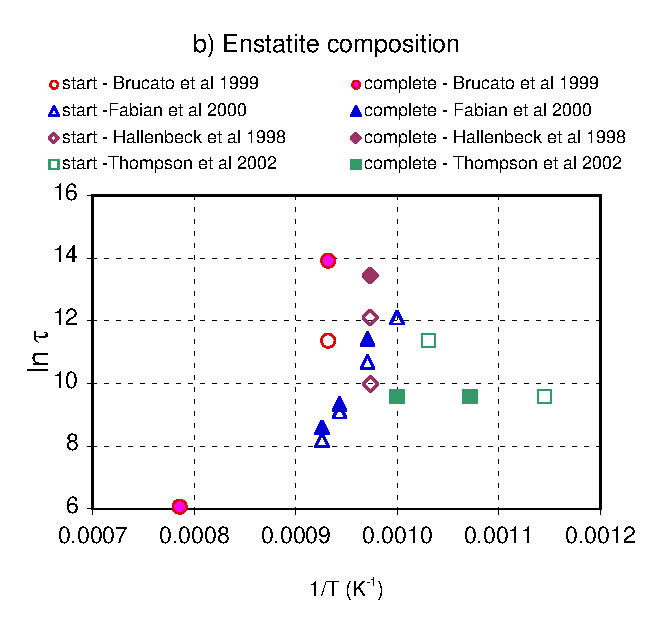
\includegraphics[width=8cm]{a1fig1a.eps}
\hspace{1em}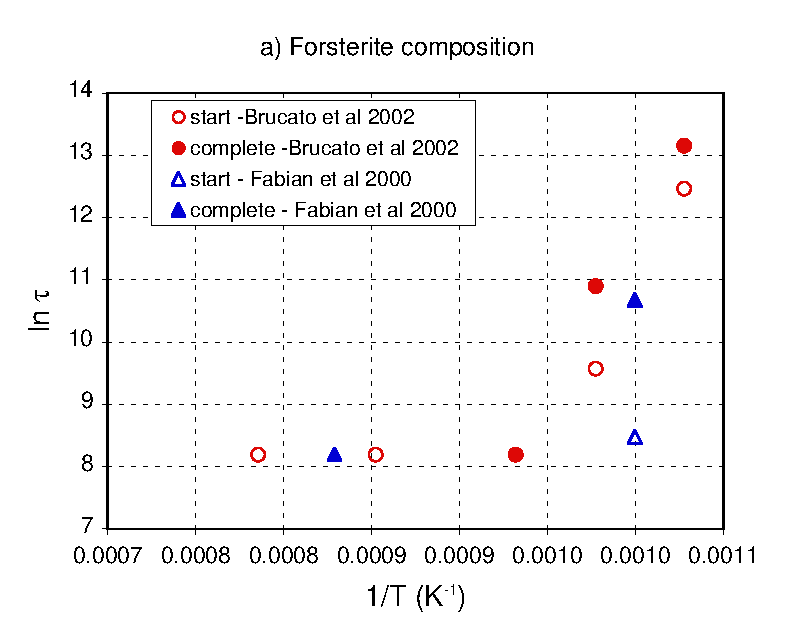
\includegraphics[width=8cm]{a1fig1b.eps}}
\caption{Characteristic annealing times ($\tau$) as a function of inverse
annealing temperature ($1/T$) for the bulk composition of forsterite (a) and
that of enstatite (b). Open symbols refer to annealing times necessary for
the first appearance of an ordered structure ($\tau_{S}$), filled symbols to
those at which crystallization appears complete ($\tau_{C}$). }
\end{figure}

\section{Preliminary work (Eigene Vorarbeiten)}

As an experimental mineralogist, PI Dominique Lattard has a longstanding
experience in high-temperature experiments in air, in vacuo or under
controlled oxygen fugacities (fO$_{2}$) on silicates and oxides, especially
on Fe-bearing phases. Such experiments were performed in the frame of very
different projects, e.g.\ to synthesize minerals, to simulate crystallization
processes from a silicate liquid, to determine the stability conditions of
single minerals or mineral assemblages as a function of temperature or
fO$_{2}$, to retrieve thermodynamic data or kinetic parameters (e.g.\ Langer
et al.\ 1977, Lattard \& Evans 1992, Lattard 1995, Lattard \& Partzsch 2001,
Lattard et al.\ 2005). D. Lattard has also the necessary expertise concerning
the mineralogical and chemical characterisation of products of
high-temperature experiments, i.e.\ with light microscopy, X-ray
diffractometry, scanning electron microscopy, electron microprobe analysis,
infrared spectroscopy, microscope-absorption-spectrophotometry, M\"ossbauer
spectroscopy (e.g.\ Langer et al.\ 1977, Langer \& Lattard, 1980, Lattard \&
Evans, 1992; Lattard 1995, Partzsch et al.\ 2004).

Co-PI Mario Trieloff has broad experience in cosmochemistry and
geochemistry, in particular with the isotope radiochronometry of processes
in the early solar system and their relationship to astrophysical processes
in protoplanetary disks. M. Trieloff conducted a number of studies on early
meteorite chronology and the accretionary history of planetesimals,
i.e.\ meteorite parent bodies (Trieloff et al.\ 2003; Pellas et al.\ 1997;
Korochantseva et al.\ 2005). He also studied processes that relate to disk
clearing and solar wind implantation into precursor planetesimals of
meteorite parent bodies and the terrestrial planets (Trieloff et al.\ 2000,
2002; Trieloff \& Kunz, 2005). Trieloff \& Palme (2006) reviewed and outlined
the early solar system history as seen by meteoriticists in the context of
astrophysical processes and disk evolution, written for and specifically
aimed at astrophysically oriented planetary scientists interested in
cosmochemistry. M. Trieloff has particular experience with high temperature
furnaces and ultra high vacuum technology for noble gas extraction from
solids, and mass spectrometric analysis, for which in-house constructed high
temperature furnaces are used. There is particular experience with general
diffusion theory (e.g.\ Trieloff et al.\ 2005), which is particularly
important if laboratory Arrhenius parameters (activation energy,
pre-exponential or frequency factor) are extrapolated from laboratory
temperature and times to parameters relevant in natural systems to be
modelled (where effects at much longer times and lower temperatures have to
be considered).

Co-PI Annemarie Pucci (before 1998 A. Lehmann) has a longstanding experience
with IR investigations of thin films with thickness in the nm range, both
with transmittance spectroscopy (for transparent substrates) and with IR
reflection of p-polarized light at grazing incidence (for metal
substrates). She used these techniques to gain information on morphology,
crystalline structure, chemical composition, impurities, and (in
semiconductors) free charge carriers of thin films (e.g.\ Lehmann et
al.\ 1982; Lehmann 1993; Priebe et al.\ 2004). In the last years A. Pucci and
her working group also studied the growth of metal films and of adsorbate
layers under UHV conditions. Important growth parameters were the metal
deposition rate adjusted via the temperature of a Knudsen cell and measured
with a quartz micro-balance and the substrate temperature. These two
parameters will be of importance in the evaporation/condensation
investigations planed in the present project. As a result of these previous
studies, the morphology development of metal growth on various substrates
was clarified and adsorbate structures could be explained (Lust et al.\ 2002;
Priebe et al.\ 2004; Pucci 2005). Also phase transitions in iron silicides
were monitored (e.g.\ Fahsold et al.\ 2002).

The amorphous thin films to be used in the annealing experiments will be
produced with the PLD setup at the Institut f\"ur Geologie, Mineralogie und
Geophysik, Ruhr-Universit\"at Bochum, in collaboration with Dr.\ Ralf Dohmen
and Prof.\ Dr.\ Sumit Chakraborty, who both have considerable experience with
thin films (both amorphous and crystalline thin films) of natural and
synthetic silicates, in particular of olivine and pyroxene compositions
(e.g.\ Dohmen et al.\ 2002).

For evaporation and condensation experiments, we envisage collaboration with
the leading expert Prof.\ H.\ Nagahara, University of Tokyo (Nagahara et
al.\ 1994; Nagahara and Ozawa 1996; Tsuchiyama et al.\ 1999; Tachibana et
al.\ 2002) and with Prof.\ S.\ Chakraborty and Dr.\ R.\ Dohmen, particularly
taking into account their previous studies (Dohmen et al.\ 1998, 2003; Dohmen
\& Chakraborty 2003) on the influence of crystal-parameters on reaction paths
and reaction rates, and considering diffusion effects.



%
% Here follows the own refereed publications by the PIs in relation to
% the project proposed here.
%
\ownpubltitle{Own publications related to the Forschergruppe:}
%
% BELOW IS ONLY AN EXAMPLE OF TWO ENTRIES. SEE THE ADDITIONAL FILES 
% SENT TO YOU WITH ALL THE REFERENCES FROM THE VORANTRAG
%
\begin{ownpubl}

\item Fahsold, G., Singer, K. and Pucci A. (2002) In-situ IR-transmission
  study of vibrational and electronic properties during the formation of
  thin-film $\beta$-FeSi$_2$. 
  \textit{Journal of Applied Physics\/}, \textbf{91}, 145
\item Korochantseva, E.V., Trieloff, M., Buikin, A.I., Meyer, H.P. and Hopp,
  J. (2005) Argon-40/Argon-39 dating, and cosmic ray exposure time of desert
  meteorites: Dhofar 300 and Dhofar 007 eucrites and anomalous achondrite NWA
  011. \textit{Meteoritics and Planetary Science\/}, \textbf{40}, 1433
\item Langer, K. and Lattard, D. (1980) Identification of a low-energy
  OH-valence vibration in zoisite. \textit{American Mineralogist\/},
  \textbf{65}, 779
\item Langer, K., Lattard, D. and Schreyer, W. (1977) Synthesis and
  stability of deerite, Fe$^{2+}$$_{12}$Fe$^{3+}$$_{6}$Si$_{12}$O$_{40}$ (OH)
  $_{10}$ and Fe$^{3+}$= Al$^{3+}$ substitutions at 15-28
  kb. \textit{Contributions to Mineralogy and Petrology \/}, \textbf{60}, 271
\item Lattard, D. (1995) Experimental evidence for the exsolution of
  ilmenite from titaniferous spinels. \textit{American Mineralogist \/},
  \textbf{80}, 968
\item Lattard, D. and Evans, B.W. (1992) New experiments on the stability of
  grunerite. \textit{European Journal of Mineralogy\/}, \textbf{4}, 218
\item Lattard, D. and Partzsch, G.M. (2001) Magmatic crystallization
  experiments at 1 bar in systems closed to oxygen: A new/old experimental
  approach. \textit{European Journal of Mineralogy \/}, \textbf{13}, 467
\item Lattard, D., Sauerzapf, U. and K\"asemann, M. (2005) New calibration
  data for the Fe-Ti oxide thermo-oxybarometers from experiments in the
  Fe-Ti-O system at 1 bar, 1000-1300 \degr C and a large range of oxygen
  fugacities. \textit{Contributions to Mineralogy and Petrology\/},
  \textbf{149}, 735
\item Lehmann, A. (1993) Information about the microcrystalline structure
  from the infrared reflection spectra of thin UV-optical films: NdF3 and
  MgF2. 
  \textit{Thin Solid Films\/}, \textbf{230}, 55
\item Lehmann, A., Schumann, L., Sobotta, H., Riede, V., Teschner, U. and
  H\"ubner, K. (1982) LO-TO Mode Splittings and Dynamic Effective Charges of
  Oxygen in Reactively Sputtered SiOx Determined by IR Spectroscopy. \textit{
  Physica status solidi (b) \/}, \textbf{111}, K103
\item Lust, A. Priebe, A., Fahsold, G. and Pucci, A. (2002) Infrared
  spectroscopic study of the CO-mediated decrease of the percolation threshold
  during the growth of ultrathin metal films on MgO(001). \textit{Surface and
  Interface Analysis \/}, \textbf{33}, 487
\item Partzsch, G.M., Lattard, D. and McCammon, C. (2004) M\"ossbauer
  spectroscopic determination of Fe$^{3+}$/Fe$^{2+}$ in synthetic basaltic
  glass: a test of empirical equations under superliquidus and subliquidus
  conditions. \textit{Contributions to Mineralogy and Petrology\/},
  \textbf{147}, 565
\item Pellas, P., Fieni, C., Trieloff, M. and Jessberger, E.K. (1997) The
  cooling history of the Acapulco meteorite as recorded by the 244Pu and
  40Ar-39Ar chronometers. \textit{Geochimica et Cosmochimica Acta\/},
  \textbf{61}, 3477
\item Priebe, A., Fahsold, G. and Pucci, A. (2004) Strong pyramidal growth
  of metal films studied with infrared spectroscopy. \textit{Journal of
  Physics and Chemistry\/}, \textbf{B 8}, 18178
\item Priebe, A., Walter, N. and Pucci, A. (2004) An IR spectroscopic study
  of silicon oxynitride films. In: \textit{Conference Digest of the 29th
  International Conference on Infrared and Millimeter Waves and of the 12th
  International Conference on Terahertz Electronics}, Karlsruhe, Germany,
  (Eds. M. Thumm, W. Wiesbeck), IEEE Catalog No.04X857, ISBN 0-78038490-3, 93
\item Pucci, A. (2005) IR spectroscopy of adsorbates on ultrathin metal
  films. \textit{Physica status solidi (b) \/}, \textbf{242}, 2704
\item Trieloff, M. and Kunz, J. (2005) Isotope systematics of noble gases in
  the Earth�s mantle: Possible sources of primordial isotopes and implications
  for mantle structure. \textit{Physics of the Earth and Planetary
  Interiors\/}, \textbf{148}, 13
\item Trieloff, M. and Palme, H. (2006) The origin of solids in the early
  solar system. In: \textit{Planet Formation - Theory, Observations, and
  Experiments}. (Eds. H. Klahr, W. Brandner), Cambridge University Press,
  Cambridge, 64
\item Trieloff, M., Falter, M., Buikin, A.I., Korochantseva, E.V.,
  Jessberger, E.K. and Altherr R. (2005) Argon isotope fractionation induced
  by stepwise heating. \textit{Geochimica et Cosmochimica Acta\/},
  \textbf{69}, 1253
\item Trieloff, M., Jessberger, E.K., Herrwerth, I., Hopp, J., Fi\'eni, C.,
  Gh\'elis, M., Bourot-Denise, M. and Pellas, P. (2003) 244Pu and 40Ar-39Ar
  thermochronometries reveal structure and thermal history of the H-chondrite
  parent asteroid. \textit{Nature\/}, \textbf{422}, 502
\item Trieloff, M., Kunz, J. and All\`egre, C.J. (2002) Noble gas systematics
  of the R\'eunion mantle plume source and the origin of primordial noble
  gases in Earth�s mantle. \textit{Earth and Planetary Science Letters\/},
  \textbf{200}, 297
\item Trieloff, M., Kunz, J., Clague, D.A., Harrison, D. and All�gre,
  C.J. (2000) The nature of pristine noble gases in mantle
  plumes. \textit{Science\/}, \textbf{288}, 1036

\end{ownpubl}
%
\section{Goals (Ziele)}
The main goal of the present project is to supply reliable laboratory data
on the physico-chemical processes taking place during evaporation,
condensation and thermal annealing of silicate minerals in proto-planetary
disks, with an emphasis on the kinetics of these processes. These data are
urgently needed for a consistent astrophysical modeling of the variations in
radial abundance of dust/minerals and of their chemical compositions at
various evolutionary stages of the protoplanetary disk. Studies will focus
on silicate minerals that are predicted by classical
condensation/evaporation sequences.  The project comprises two parts:

\begin{enumerate}
\item {\em Laboratory simulation of the crystallization} of amorphous silicate
components in cosmic dust during thermal annealing incl.\ determination of
reliable kinetic parameters. As the crystallization state of Fe-containing
olivine and pyroxene are expected to have the strongest influence on
extinction properties in protoplanetary disks, priority will be given to
forsterite-fayalite solid solution, and enstatite-ferrosilite solid
solution, but Ca-rich pyroxenes (diopside) will also be considered. Special
attention will be given to the preparation of amorphous material by
different methods (Pulsed Laser Deposition, glasses, gels).

\item {\em Laboratory determination of parameters for evaporation and
condensation} of dust/minerals under conditions relevant for protoplanetary
disks by heating and condensation experiments. Here, also some complementary
studies (where data are missing) will be performed on Fe-containing olivine
and pyroxene, but from the beginning we shall also focus on Ca, Al compounds
that are the only minerals in high temperature regions and important
carriers for many refractory elements at high temperatures (e.g.\ spinel,
hibonite, melilite, anorthite, diopside) and volatile elements at lower
temperatures (plagioclase, diopside). The first experiments will focus on
melilite solid solution of gehlenite-akermanite.

\end{enumerate}
%
These experiments are aimed to yield results for conditions relevant to
protoplanetary disks, e.g.\ temperature, redox state, pressure. An important
part to improve previous data are a) long-term experiments to get more
precise data for extrapolation to longer time intervals relevant in
protoplanetary discs b) extension of the experiments to cover more realistic
mineral compositions. Another improvement is attempted in the thorough
analytical characterization of starting materials and experimental outcome
material by micro-analytical tools like atomic force microscopy (AFM),
transmission and secondary electron microscopy (TEM; SEM), electron
microprobe (EMPA) and possibly ion microprobe (SIMS).

One of the strength of our project is the interdisciplinary cooperation
between astrophysicists, cosmochemists, mineralogists, experimental
physicists, who all contribute their specific expertise.


\section{Work schedule (Arbeitsprogramm)}
\subsection{Methods}
\subsubsection{Part 1 (Annealing):}

We plan to perform high-temperature (800-1200 K) annealing experiments on
iron-free and iron-bearing olivines - (Mg,Fe) $_{2}$SiO$_{4}$ -,
orthopyroxenes - (Mg,Fe)SiO$_{3}$ -, and clinopyroxenes - Ca
(Mg,Fe)Si$_{2}$O$_{6}$.

\paragraph{Amorphous starting materials:}

We shall particularly care for chemically homogeneous, structurally and
morphologically well-characterized amorphous starting materials. Our
emphasis will be on thin films produced by Pulsed Laser Deposition (PLD),
which fulfill these criteria in order to mimic amorphous cosmic dust. The
thin films will be produced with the PLD setup at the Institut f\"ur
Geologie, Mineralogie und Geophysik, Ruhr-Universit\"at Bochum, in
collaboration with Dr.\ Ralf Dohmen and Prof.\ Sumit Chakraborty.

The set up at Bochum has been custom designed for mineralogical applications
and includes an excimer Laser working with either ArF, KrF or XeF gas
mixtures, which leads to wavelengths of 193, 248 or 351 nm. For example,
with KrF the laser produces pulse energies up to 1400 mJ at a maximum
frequency of 50 Hz (pulse duration of 30 ns). The system can be operated at
high vacuum conditions of up to 10-5 Pa. This high vacuum background allows
the use of a flow of oxygen or of other gases with varying partial
pressure. This is of great advantage in order to avoid evaporation of Mg or
to control the redox condition of Fe (e.g.\ articles in Chrisey \& Hubler,
1994).

As targets for the laser beam, we shall essentially use dense pressed
polycrystalline pellets of the synthetic phase of interest, i.e.\ olivine,
pyroxene. In case of Fe$^{2+}$-bearing phases, these pellets will be
synthesized at high temperatures under oxygen fugacities controlled by
CO/CO$_2$ gas mixtures, in order to obtain the desired oxidation state of
iron (standard techniques in the working group of D. Lattard). We shall also
test high purity reagent mixtures (oxides, metals) on the desired
compositions.  As substrates to be coated with the thin films, we plan to
test spec. pure graphite, silicon crystal wafers, ceramic platelets
(e.g.\ Al$_{2}$O$_{3}$, ZrO$_{2}$) and synthetic polished and oriented single
crystals (commercially available, e.g.\ from Crystec GmbH).

Dohmen et al.\ (2002) have shown through thorough characterization with
different techniques (e.g.\ SEM, TEM, white light interference microscopy,
Rutherford Backscattering (RBS)) that the silicate thin films produced with
the PLD set up in Bochum are amorphous, highly uniform in thickness ($\pm$ 1
nm), chemically homogeneous and of the desired chemical composition. In some
cases the composition of the thin film is slightly more enriched in oxygen
than the target composition. Recent studies of the Bochum group have shown
that this problem may be corrected by reducing the background pressure in
the deposition chamber. This possibility is particularly important in case
of Fe-bearing compositions. In the mean time, amorphous thin films with
various Fe/Mg values on olivine and orthopyroxene compositions have been
routinely produced with the set-up in Bochum (Dohmen, pers. communication,
2006).

The first characterization of the amorphous thin films will be performed
with RBS, which enables measurements of both the chemical composition and
the thickness of the thin films (Dohmen et al.\ 2002). RBS measurements will
be carried out at the Dynamitron Tandem Laboratorium of the
Ruhr-Universit\"at Bochum in cooperation with Dr. Hans-Werner
Becker. Further characterization of the thin films with SEM and atomic force
microscopy (surface properties), with micro-analytical methods (chemistry)
and with IR spectroscopy will be performed at the mineralogical institute
and at the KIP.

For comparison we shall also use other homogeneous amorphous starting
materials, namely glasses and gels. Gels are relatively easily prepared
(e.g.\ Hamilton \& Henderson, 1968), but one has to take into account that
they contain iron in the trivalent state. In contrast, in Fe-bearing glasses
redox state of iron can be adjusted by equilibrating the silicate melt under
controlled fO$_{2}$ conditions in a furnace with a flowing CO/CO$_{2}$ gas
mixture (cf.\ Partzsch et al.\ 2004). Glasses in the Fe-Mg-Si-O system,
however, have to be prepared and examined with great care because of their
tendency to very rapidly crystallize during quenching (e.g.\ Boyd \& Schairer,
1964).

\paragraph{Annealing procedure}

We have two main options to realize annealing of the amorphous materials.
\begin{itemize}
\item Annealing at temperatures in the range 800-1200 K in vertical quench
furnaces under controlled atmosphere (air, CO/CO$_{2}$ gas mixtures) or in
vacuo (evacuated silica glass tubes) for well-defined run durations
(standard techniques at the Mineralogical Institute). Quench and subsequent
characterization of the run products with IR spectroscopy, X-ray
diffraction, and micro-analytical methods (SEM, electron microprobe, TEM,
etc.). Details on the experimental and analytical methods can be found
e.g.\ in Lattard et al.\ (2005).
\item Annealing in the experimental setup for IR spectroscopy under UHV
conditions (10$^{-8}$ Pa) at the KIP with in situ characterization of the
progress of crystallization of thin films with thickness in the nm range (up
to several 100 nm). Sample heating up to 1400 K is possible. Depending on
the sample size and the sample-holder construction, these temperatures can
be reached within seconds to minutes. Gas exposure (CO, CO$_{2}$, O$_{2}$)
up to a partial pressure of 2x10$^{-6}$ Pa can be performed in the UHV
chamber. The IR investigations of thin films can be performed either with
transmittance spectroscopy in the case of transparent substrates or with IR
reflection of p-polarized light at grazing incidence in the case of metal
substrates. Phonons in wafer-like samples with thickness in the micron range
and above are studied with reflectance spectroscopy. Above the phonon
absorption edge, transmittance studies can give information on impurities
and optical properties.
\end{itemize}

Even if annealing is performed in quench furnaces, IR investigations of thin
film run products can be performed in the experimental setup for IR
spectroscopy at KIP. In contrast to IR spectra retrieved from KBr pellets
(e.g.\ Brucato et al.\ 1999, Thompson et al.\ 2002), the artificial matrix
effects are avoided, giving clearer results on vibration properties. For
comparison, however, some IR spectra from powdered samples embedded in KBr
should also be measured in the sample chamber of the IR spectrometer at the
KIP and with other conventional IR spectrometers. We also plan in-situ
synchrotron IR investigations during annealing of short durations (e.g.\ at
temperatures around 1200 K) at the ANKA-Synchrotron (Karlsruhe).

To better define the progress of crystallization, we shall examine selected
annealed samples with the TEM, in collaboration with specialists
(Dr. F. Brenker, Universit\"at Frankfurt). We shall also analyze
recrystallized samples with RBS to exclude any reaction with the synthetic
substrates and to confirm that re-crystallization of the film is the only
process investigated.


\subsubsection{Part 2 (Evaporation/condensation):}

Experimental data for evaporation and condensation rates primarily exist
only for the Mg-rich silicates forsterite and enstatite. Few is known about
the important Fe-bearing olivine and pyroxene, or Ca, Al compounds, i.e.\ the
high temperature condensates corundum, hibonite, spinel, melilite, or at
slightly lower temperatures anorthite and diopside, and finally carrier
minerals of moderately volatile elements (e.g.\ Alkalis, Mn) like
plagioclase. For this reason, first experiments are planned on Fe-containing
olivine and pyroxene (Fo 60-100, En 60-100), and Ca, Al silicates (melilite
solid solution, diopside, plagioclase)

\begin{itemize}
\item As starting materials we will use either synthesized, commercially
available (e.g.\ Crystec GmbH, Berlin/ SPI supplies) or natural materials
(SPI Supplies/C.M. Taylor collection). They will be checked for homogeneity
and purity by EMP and possibly by ion microprobe. We expect to succeed in
obtaining appropriate material, however, in the case these materials have
not the desired level of homogeneity and purity, the synthesis of crystals
can also be performed by high temperature experiments under controlled
oxygen fugacity, either via solid state reactions or in the presence of a
melt phase or a flux. Respective high temperature furnaces are available at
the Mineralogical Institute, or via cooperations with labs specialized in
mineral synthesis.
\item Experiments with larger samples can be performed in ultra high vacuum
lines, using either resistance heated high temperature furnaces (up to 2000
\degr C) at the Min.\ Inst.\ or - alternatively - the experimental setup at
the KIP. This set up includes an electron impact heated furnace, from where
material can be evaporated and condensed as a thin film onto substrates that
are kept at specific temperatures. During condensation the film can be
characterized with IR spectroscopy. Gases (e.g.\ hydrogen) can be admixed on
both experimental facilities to simulate pressure and/or gas/dust ratios
relevant for protoplanetary disks. With this setup, partial pressures in the
UHV range, temperatures for evaporation up to 2000 K and for condensation up
to about 1400 K (see above) are possible. The photometric sensitivity is
sufficient to investigate phonon bands of condensed films with thickness in
the nm range. Evaporation rates are independently determined with a quartz
microbalance. The film morphology can be checked ex-situ with atomic force
microscopy (NanoScopeIV).
\item Equilibrium experiments with a Knudsen cell are necessary to clarify
phase relationships in some systems, e.g.\ for melilite solid solution with
the endmembers gehlenite and akermanite (evaporation dependent on chemical
composition and pressure, check for the occurrence of melts, check for
incongruent evaporation, see Hashimoto, 1990). Non-equilibrium experiments
(Langmuir configuration) to determine evaporation and condensation
coefficients will be performed afterwards. Evaporated material can be
condensed as thin films on a substrate kept at constant temperature. In the
case of olivine, phase relationships are principally clarified, however,
additional experiments at lower temperatures and longer laboratory times are
planned to verify and precise the kinetic parameters. Similarly, such
experiments must be performed for pyroxene solid solution between the
enstatite and ferrosilite endmembers. Particular attention has to be paid to
the control of oxygen fugacity. As an example oxygen fugacity can be
controlled by using a Mo capsule as Knudsen cell. Molybdenum reacts with
oxygen in the sample to form MoO$_{2}$. The fO$_{2}$ of the Mo-MoO$_{2}$
buffer is between that of the iron-w\"ustite (IW) and w\"ustite-magnetite
(WM) buffers (Mysen \& Kushiro 1988). The MoO$_{2}$ gas is not reactive
with the experimental system.
\item For the characterization of the experimental products a broad range of
micro-analytical facilities exists, e.g.\ atomic force microscopy at KIP or
optical and electron microscopy, electron microprobe, ion microprobe, X-ray
diffractometry at the Mineralogical Institute.
\end{itemize}
%
The experiments will be performed in collaboration with the leading expert
Prof. H. Nagahara, University of Tokyo. Cooperation is also envisaged with
Profs. S. Chakraborty and R. Dohmen, particularly taking into account their
previous studies (Dohmen et al.\ 1998, 2003; Dohmen \& Chakraborty 2003) that
have shown that crystal size or grain size of polycrystalline material
compared to the interacting reservoir also define reaction paths and, hence,
reaction rates. Moreover, diffusion may also play a role. Quantitative
modelling has to take into account these effects.



\subsection{Schedule Student 1 (Annealing)}
\subsubsection{First year}
Preparation and characterization (RBS, SEM, IR-spectroscopy) of amorphous
starting materials on the composition of Fe-free and Fe-bearing olivine,
(Fe,Mg) $_{2}$SiO$_{4}$, and of orthopyroxene, (Fe,Mg)SiO$_{3}$. The
emphasis will be on thin films prepared with the PLD method, but gels and
some Fe-bearing glasses should also be prepared for comparison.  First
annealing experiments in vertical quench furnaces. They will be performed in
air and in vacuum for Fe-free compositions, in vacuum and under different,
controlled oxygen fugacities for Fe-bearing compositions. Characterization
of the run products with RBS, SEM, EMP, IR-spectroscopy, TEM.  Preparation
and first tests of in-situ annealing in the experimental setup for IR
spectroscopy under UHV conditions and data analysis.

\subsubsection{Second year}
Preparation of amorphous starting materials on clinopyroxene compositions
(Ca(Fe,Mg) Si$_{2}$O$_{6}$). Further annealing experiments on different
compositions in quench furnaces and in the experimental setup for IR
spectroscopy under UHV conditions. Test of in-situ IR synchrotron
experiments at ANKA.


\subsubsection{Third year}
Final experiments. Extensive data analysis. Preparation of publications/PhD
thesis.

\subsection{Schedule Student 2 (Evaporation/Condensation)}
\subsubsection{First year}
Preparation and characterization of crystalline starting materials for
evaporation/ condensation experiments (Fe-containing olivine and pyroxene of
Fo 60-100, En 60-100, and Ca,Al silicates, i.e.\ melilite solid solution,
diopside, plagioclase). Evaporation/condensation experiments with Fe-bearing
olivine and pyroxene. Test of Ca, Al-bearing minerals and improvement of
experimental setup for high temperature experiments on Ca, Al minerals
(e.g.\ heating of condensation substrates). Characterization of condensation
products and evaporation residues by SEM, X-ray, electron microprobe, AFM,
and possibly also IRS. For this purpose, some experimental modification is
necessary regarding sample holder construction, and evaporator crucible
test.
\subsubsection{Second year}
Evaporation/condensation experiments for refractory Ca, Al bearing minerals.
\subsubsection{Third year}
Final experiments. Preparation of publications/PhD thesis.


\subsection{Literature}
%
% Here follows a general literature list related to the topic of the
% proposal, just like a literature list for a scientific paper.
%
% AGAIN ONLY EXAMPLES ARE LISTED NOW
%
\begin{literature}
\item Alexander, C.M.O., Boss, A.P., Keller, L.P., Nuth, J.A. and
  Weinberger, A. (2006) Astronomical and meteoritic evidence for the nature
  of interstellar dust and its processing in protoplanetary disks. In:
  \textit{Protostars and Planets V}, (Eds. B. Reipurth, D. Jewitt,
  K. Keil). \\ 
  {\tt http://ifa.hawaii.edu/UHNAI/ppv.htm}
\item All\`egre, C.J., Manh\`es, G. and Lewin, E. (2001) Chemical
  composition of the earth and the volatility control on planetary
  genetics. \textit{Earth and Planetary Science Letters\/}, \textbf{185}, 49
\item Apai, D. and Pascucci, I. and Bouwman, J. and Natta, A. and Henning,
  T. and Dullemond, C. P. (2005) The Onset of Planet Formation in Brown
  Dwarf Disks, \textit{Science\/}, \textbf{310}, 834
\item Bell, K.R., Cassen, P.M., Klahr, H.H. and Henning, T. (1997) The
  structure and appearance of protostellar accretion disks: limits on disk
  flaring. \textit{Astrophysical Journal\/}, \textbf{486}, 372
\item Bell, K.R. and Linn, D.N.C. (1994) Using FU Orionis outbursts to
  constrain self-regulated protostellar disk models. \textit{The Astrophysical
  Journal\/}, \textbf{427}, 987
\item Bergin, E.A., Aikawa, Y., Blake, D.A., and von Dishoeck, E.F. (2006)
  The chemical evolution of protoplanetary disks. In: \textit{Protostars and
  Planets V}, (Eds. B. Reipurth, D. Jewitt, K. Keil),\\ 
  {\tt http://ifa.hawaii.edu/UHNAI/ppv.htm}
\item Bockel\'ee-Morvan, D., Gautier, D., Hersant, F., Hur�, J.M., and Robert,
  F. (2002) Turbulent radial mixing in the solar nebula as the source of
  crystalline silicates in comets. \textit{Astronomy and Astrophysics\/},
  \textbf{384}, 1107
\item Boekel, R. van et al.\ (2004) The building blocks of planets within the
  'terrestrial' region of protoplanetary disks \textit{Nature\/},
  \textbf{432}, 479
\item Boffa Ballaran, T., Carpenter, M.A. and Ross, N.L. (2001) Infrared
  powder-absorption spectroscopy of Ca-free P21/c
  clinopyroxenes. \textit{Mineralogical Magazine\/}, \textbf{65}, 339
\item Boss, A. P. (2004) Evolution of the Solar Nebula. VI. Mixing and
  Transport of Isotopic Heterogeneity. \textit{Astrophysical Journal\/},
  \textbf{616}, 1265-1277
\item Bouwman, J., Meeus, G., de Koter, A., Hony, S., Dominik, C. and
  Waters, L.B.F.M. (2001) Processing of silicate dust grains in Herbig Ae/Be
  systems. \textit{Astronomy and Astrophysics\/}, \textbf{375}, 950-962.
\item Boyd, F.R. and Schairer, J.F. (1964): The system
  MgSiO$_{3}$-CaMgSi$_{2}$O$_{6}$. \textit{Journal of Petrology\/},
  \textbf{5}, 275
\item Bowen, N.L. and Schairer, J.F. (1935) The system
  MgO-FeO-SiO$_{2}$. \textit{American Journal of Science\/}, \textbf{29},
  151
\item Brucato, J.R., Colangeli, L., Mennella, V., Palumbo, P. and
  Bussoletti, E. (1999) Mid-infrared spectral evolution of thermally annealed
  amorphous pyroxene. \textit{Astronomy and Astrophysics\/}, \textbf{348},
  1012
\item Brucato, J.R., Mennella, V., Colangeli, L., Rotundi, A. and Palumbo,
  P. (2002) Production and processing of silicates in laboratory and in
  space. \textit{Planetary and Space Science\/}, \textbf{50}, 829
\item Chihara, H., Koike, C., Tsuchiyama, A., Tachibana, S., and Sakamoto,
  D. (2002) Compositional dependence of infrared absorption spectra of
  crystalline silicate. I. Mg-Fe pyroxenes. \textit{Astronomy and
  Astrophysics\/}, \textbf{391}, 267
\item Chrisey, D.B. and Hubler, G.K. (1994) Pulsed laser deposition of thin
  films, p. 613. John Wiley and Sons.
\item D'Alessio, P., Calvet, N. and Woolum, D.S. (2005) Thermal structure of
  protoplanetary disks. In: \textit{Chondrites and the protoplanetary disk\/},
  ASP Conf. Ser. Vol. 341 (Eds. A.N. Krot, E.R.D. Scott, B. Reipurth), 353
\item Dohmen, R. and Chakraborty, S. (2003) Mechanism and kinetics of
  element and isotopic exchange mediated by a fluid phase. \textit{American
  Mineralogist}, 88, 1251-1270.
\item Dohmen, R., Becker, H.-W., Meissner, E., Etzel, T. and Chakraborty,
  S. (2002) Production of silicate thin films using pulsed laser deposition
  (PLD) and applications to studies in mineral kinetics. \textit{European
  Journal of Mineralogy\/}, \textbf{14}, 1155
\item Dohmen, R. and Chakraborty, S. (2003) Mechanism and kinetics of
  element and isotopic exchange mediated by a fluid phase. \textit{American
  Mineralogist\/}, \textbf{88}, 1251
\item Dohmen, R., Chakraborty, S., Palme, H. and Rammensee, W. (1998)
  Solid-solid reactions mediated by a gas phase: An experimental study of
  reaction progress and the role of surfaces in the system olivine+iron
  metal. \textit{American Mineralogist\/}, \textbf{83}, 970
\item Dohmen, R., Chakraborty, S., Palme, H. and Rammensee, W. (2003) Role
  of element solubility on the kinetics of element partitioning: In situ
  observations and a thermodynamic kinetic model. \textit{Journal of
  Geophysical Research\/}, \textbf{108}, 2157
\item Dorschner, J., Begemann, B., Henning, T., J\"ager, C. and Mutschke,
  H. (1995) Steps toward interstellar silicate mineralogy. II.  Study of
  Mg-Fe-silicate glasses of variable composition. \textit{Astronomy and
  Astrophysics\/}, \textbf{300}, 503
\item {Dullemond}, C.~P., {Apai}, D. and {Walch}, S. (2006)
  Crystalline Silicates as a Probe of Disk Formation History, 
  \apjl \textbf{640}, 67
\item Duschl, W.J., Gail, H.P. and Tscharnuter, W.M. (1996) Destruction
  processes for dust in protoplanetary accretion disks. \textit{Astronomy and
  Astrophysics\/}, \textbf{312}, 624
\item Fabian, D., J\"ager, C., Henning, T., Dorschner, J. and Mutschke,
  H. (2000) Steps toward interstellar silicate mineralogy. V. Thermal
  evolution of amorphous magnesium silicates and silica. \textit{Astronomy and
  Astrophysics\/}, \textbf{364}, 282
\item Gail, H.P. (1997) Chemical reactions in protoplanetary disks IV. Multi
  component dust mixture. \textit{Astronomy and Astrophysics\/}, \textbf{332},
  1099
\item Gail, H.P. (2001) Radial mixing in protoplanetary accretion disks
  I. Stationary disk models with annealing and carbon
  combustion. \textit{Astronomy and Astrophysics\/}, \textbf{378}, 192
\item Gail, H.P. (2003) Formation and evolution of minerals in accretion
  disks and stellar outflows. In: \textit{Astromineralogy}, Lecture Notes in
  Physics (Ed. T. Henning) Springer, Heidelberg, 55
\item Gail, H.P. (2004) Radial mixing in protoplanetary accretion disks
  IV. Metamorphosis of the silicate dust complex. \textit{Astronomy and
  Astrophysics\/}, \textbf{413}, 571
\item J\"ager, C., Molster, F.J., Dorschner, J., Henning, T., Mutschke, H.,
  and Waters, L.B.F.M. (1998) Steps toward interstellar silicate
  mineralogy. IV. The crystalline revolution. \textit{Astronomy and
  Astrophysics\/}, \textbf{339}, 904
\item J\"ager, C., Dorschner, J., Mutschke, H., Posch, T., and Henning,
  T. (2003) Steps toward interstellar silicate mineralogy. VII.  Spectral
  properties and crystallization behaviour of magnesium silicates produced by
  the sol-gel method. \textit{Astronomy and Astrophysics\/}, \textbf{408}, 193
\item Hallenbeck, S. L.; Nuth, J. A. and Daukantas, P. L. (1998)
  Mid-Infrared spectral evolution of amorphous Magnesium silicate smokes
  annealed in vacuum: Comparison to cometary spectra. \ica, \textbf{131}, 198
\item Hamilton, D.L. and Henderson, C.M.B. (1968) The preparation of
  silicate compositions by a gelling method. \textit{Mineralogical
  Magazine\/}, \textbf{36}, 832
\item Harker, D.E. and Desch, S.J. (2002) Annealing of silicate dust by
  nebular shocks at 10 AU. \textit{Astrophysical Journal Letters\/},
  \textbf{565}, L109
\item Harker, D.E., Woodward, C.E., and Wooden, D.H. (2005) The dust grains
  from 9P/Tempel 1 before and after the encounter with deep
  impact. \textit{Science\/}, \textbf{310}, 278
\item Hashimoto, A. (1990) Evaporation kinetics of forsterite and
  implications for the early solar nebula. \textit{Nature\/}, \textbf{374}, 53
\item Hashimoto, A. (1991) Evaporation of melilite. \textit{Meteoritics\/},
  \textbf{26}, 344.
\item Hofmeister, A.M. (1987) Single-crystal absorptiobn and reflection
  infrared spectroscopy of forsterite and fayalite. \textit{Physics and
  Chemistry of Minerals\/}, \textbf{14}, 499
\item Hofmeister, A.M. (1997) Infrared reflectance spectra of fayalite, and
  absorption data from assorted olivines, including pressure and isotope
  effects. \textit{Physics and Chemistry of Minerals\/}, \textbf{24}, 535
\item J\"ager, C., Molster, F.J., Dorschner, J., Henning, T., Mutschke,
  H. and Waters, L.B.F.M. (1998) Steps toward interstellar silicate
  mineralogy. IV. The crystalline revolution. \textit{Astronomy and
  Astrophysics\/}, \textbf{339}, 904
\item J\"ager, C., Dorschner, J., Mutschke, H., Posch, T. and Henning,
  T. (2003) Steps toward interstellar silicate mineralogy. VII.  Spectral
  properties and crystallization behaviour of magnesium silicates produced by
  the sol-gel method. \textit{Astronomy and Astrophysics\/}, \textbf{408}, 193
\item Kemper F., Vriend W.J., Tielens A.G.G.M. (2004). The Absence of
  Crystalline Silicates in the Diffuse Interstellar
  Medium. \textit{Astrophys. J. \/}, \textbf{609}, 826
\item Kemper F., Vriend W.J., Tielens A.G.G.M. (2004). ERRATUM: The Absence of
  Crystalline Silicates in the Diffuse Interstellar
  Medium. \textit{Astrophys. J. \/}, \textbf{633}, 534
\item Klahr, H. H., Henning, Th. and Kley, W. (1999) On the Azimuthal
  Structure of Thermal Convection in Circumstellar
  Disks. \textit{Astrophysical J. \/}, \textbf{514}, 325-343.
\item Koch-Muller, M. (1997) Experimentally determined Fe-Mg exchange
  between synthetic staurolite and garnet in the system
  MgO-FeO-Al2O3-SiO2-H2O. \textit{Lithos\/}, \textbf{41}, 185
\item Koike, C., Tsuchiyama, A., Shibai, H., Suto, H., Tanab�, T., Chihara,
  H., Sogawa, H., Mouri, H. and Okada, K. (2000) Absorption spectra of Mg-rich
  Mg-Fe and Ca pyroxenes in the mid- and far-infrared
 regions. \textit{Astronomy and Astrophysics\/}, \textbf{363}, 1115
\item Koike, C., Chihara, H., Tsuchiyama, A., Suto, H., Sogawa, H. and
  Okuda, H. (2003) Compositional dependence of infrared absorption spectra of
  crystalline silicate. II. Natural and synthetic olivines. \textit{Astronomy
  and Astrophysics\/}, \textbf{399}, 1101
\item Lattard, D., Sauerzapf, U. and K\"asemann, M. (2005) New calibration
  data for the Fe-Ti oxide thermo-oxybarometers from experiments in the
  Fe-Ti-O system at 1 bar, 1000-1300�C and a large range of oxygen
  fugacities. \textit{Contributions to Mineralogy and Petrology\/},
  \textbf{149}, 735
\item Lindsley, D.H., Davis, B.T.C. and MacGregor, I.D. (1964) Ferrosilite
  (FeSiO3) synthesis at high pressures and temperatures. \textit{Science\/},
  \textbf{149}, 735
\item Meeus, G., Waters, L.B.F.M., Bouwman, J., van den Ancker, M. E.,
  Waelkens, C. \& Malfait, K. (2001) ISO spectroscopy of circumstellar dust in
  14 Herbig Ae/Be systems: Towards an understanding of dust processing,
  \textit{Astron. \& Astrophys. \/}, \textbf{365}, 476
\item Messenger, S., Keller, L.P., Stadermann, F.J., Walter, R.M., and
  Zinner, E. (2003) Samples of stars beyond the solar system: Silicate grains
  in interplanetary dust. \textit{Science\/}, \textbf{300}, 105
\item Molster, F.J., Waters, L.B.F.M., and Tielens, A.G.G.M. (2002)
  Crystalline silicate dust around envolved stars. II. The crystalline
  silicate complexes. \textit{Astronomy and Astrophysics\/}, \textbf{382}, 222
\item Morfill, G. E. and V\"olk, H. J. (1984) Transport of dust and vapor and
  chemical fractionation in the early protosolar cloud. \textit{Astrophysical
  J. \/}, \textbf{287}, 371-395
\item Mysen, B.O. and Kushiro, I. (1988) Condensation, evaporation, melting,
  and crystallization in the primitive solar nebula: Experimental data in
  the system MgO-SiO$_2$-H$_2$ to $1.0x10^{-9}$ bar and 1870\degr C with
  variable oxygen fugacity. \textit{American Mineralogist\/}, \textbf{73}, 1
\item Mysen, B.O. and Kushiro, I. (1989) Oxygen fugacity and evaporation
  phase relations in the solar nebula. \textit{Annual Reports of the
  Geophysical Laboratory\/}, 1988-1989, 33
\item Nagahara, H., Kushiro, I., and Mysen, B.O. (1994) Evaporation of
  olivine: Low pressure phase relations of the olivine system and its
  implication for the origin of chondritic components in the solar
  nebula. \textit{Geochimica et Cosmochimica Acta\/}, \textbf{58}, 1951
\item Nagahara, H. and Ozawa, K. (1996) Evaporation of forsterite in H2
  gas. \textit{Geochimica et Cosmochimica Acta\/}, \textbf{60}, 1445
\item Natta, A., Testi, L., Calvet, N., Henning, Th., Waters, L.\ B.\ F.\ M.
  and Wilner, D. (2006) Dust in Protoplanetary disks: properties
  and evolution. In: \textit{Protostars and Planets V}, (Eds. 
  B. Reipurth, D. Jewitt, K. Keil).\\ 
  {\tt http://ifa.hawaii.edu/UHNAI/ppv.htm} 
\item Nelson, R., Thiemens, M., Nuth, J. and Donn, B. (1989) Oxygen isotopic
  fractionation in the condensation of refractory smokes. \textit{Proceedings
  Lunar Planetary Sciene conference\/}, \textbf{19}, 559
\item Nuth, J.A., Rietmeijer, F.J.M., Hallenbeck, S.L., Withey, P.A. and
  Ferguson, F. (2000) Nucleation, growth, annealing and coagulation of
  refractory oxides and metals: Recent experimental progress and applications
  to astrophysical systems. In: \textit{Thermal emission spectroscopy and
  analysis of dust, disks, and regoliths}, ASP conference Series, Vol. 196,
  (Eds. M.L. Sitko, A.L. Sprague, D.K. Lynch), 313
\item Palme, H. (2001).Chemical and isotopic heterogeneity in protosolar
  matter. \textit{Phil. Trans. R. Soc. Lond.} \textbf{A 359}, 2061--2075.
\item Paques-Ledent, M.T. and Tarte, P. (1973) Vibrational studies of
  olivine type compounds. I. The IR and Raman spectra of the isotopic species
  of Mg2SiO4. \textit{Spectrochimica Acta\/}, \textbf{29A}, 1007
\item Partzsch, G.M., Lattard, D. and McCammon, C. (2004) M\"ossbauer
  spectroscopic determination of Fe3+/Fe2+ in synthetic basaltic glass: a test
  of empirical fO2 equations under superliquidus and subliquidus
  conditions. \textit{Contributions to Mineralogy and Petrology\/},
  \textbf{147}, 565
\item Reynard, B. (1991) Single-crystal infrared reflectivity of pure
  Mg$_2$SiO$_4$ forsterite and (Mg0.86,Fe0.14)2SiO$_4$ olivine - new data and a
  reappraisal. Physics and Chemistry of Minerals\/, \textbf{18}, 19
\item Rotundi, A., Brucato, J.R., Colangeli, L., Ferrini, G., Mennella, V.,
  Palomba, E. and Palumbo, P. (2002) Production, processing and
  characterization techniques fo cosmic dust analogues. \textit{Meteoritics
  and Planetary Science\/}, \textbf{37}, 1623
\item Scott, A. and Duley, W.W. (1996) Ultraviolet and Infrared refractive
  indices of amorphous silicates. \textit{The Astrophysical Journal\/},
  \textbf{105}, 401
\item Smith, D. (1971) Stability of the assemblage iron-rich
  orthopyroxene-olivine-quartz. \textit{American Journal of Science\/},
  \textbf{271}, 370
\item Stephens, J.R. and Russel, R.W. (1979) Emission and extinction of
  ground and vapor-condensed silicates from 4 to 14 microns and the 10 micron
  silicate feature. \textit{The Astrophysical Journal\/}, \textbf{228}, 780
\item Tachibana, S., Tsuchiyama, A., and Nagahara, H. (2002) Experimental
  study of incongruent evaporation kinetics of enstatite in vacuum and in
  hydrogen gas. \textit{Geochimica et Cosmochimica Acta\/}, \textbf{66}, 713
\item Thompson, S.P., Fonti, S., Verrienti, C., Blanco, A., Orono, V., and
  Tang, C.C. (2002) Laboratory study of annealed amorphous MgSiO3 silicate
  using IR spectroscopy and synchrotron X-ray diffraction. \textit{Astronomy
  and Astrophysics\/}, \textbf{395}, 705
\item Thompson, S.P., Fonti, S., Verrienti, C., Blanco, A., Orono, V., and
  Tang, C.C. (2003) Crystalline comet dust: Laboratory experiments on a simple
  silicate system. \textit{Meteoritics and Planetary Science\/}, \textbf{38},
  457
\item Tielens A.G.G.M., Waters L.B.F.M. and Bernatowicz T.J. (2006) Origin
  and evolution of dust in circumstellar and interstellar environments. In:
  \textit{Chondrites and the protoplanetary disk\/}, ASP Conf. Ser. Vol. 341
  (Eds. A.N. Krot, E.R.D. Scott, B. Reipurth), 605.
\item Trieloff, M. and Palme, H. (2006) The origin of solids in the early
  solar system. In: \textit{Planet Formation - Theory, Observations, and
  Experiments}, (Eds. H. Klahr, W. Brandner), Cambridge University Press,
  Cambridge, 64
\item Tsuchiyama, A., Tachibana, S. and Takahashi, T. (1999) Evaporation of
  forsterite in the primordial solar nebula; rates and accompanied isotopic
  fractionation. \textit{Geochimica et Cosmochimica Acta\/}, \textbf{63}, 2451
\item Turner, N. J., Willacy, K., Bryden, G. and Yorke, H. W. (2006)
  Turbulent Mixing in the Outer Solar Nebula. \textit{Astrophysical J. \/},
  \textbf{ 639}, 1218-1226.
\item Wang, J., Davis, A.M., Clayton, R.N. and Hashimoto, A. (1999)
  Evaporation of single crystal forsterite: Evaporation kinetics, magnesium
  isotope fractionation, and implications of mass-dependent isotopic
  fractionation of a diffusion-controlled reservoir. \textit{Geochimica et
  Cosmochimica Acta\/}, \textbf{63}, 953
\item Wehrstedt, M. and Gail, H.P. (2002) Radial mixing in protoplanetary
  accretion disks. II. Time dependent disk models with annealing and carbon
  combustion. \textit{Astronomy and Astrophysics\/}, \textbf{385}, 181
\item Wehrstedt, M. and Gail, H.P. (2003) Radial mixing in protoplanetary
  accretion disks V. Models with different element mixtures. \textit{Astronomy
  and Astrophysics\/}, \textbf{410}, 917
\item Wooden, D.H., Harker, D., Woodward, C.E., Butner, H.M., Koike, C.,
  Witteborn, F.C. and McMurtry, C.W. (1999) Silicate mineralogy of the dust in
  the inner coma of comet C/1995 01 (Hale-Bopp) pre- and
  post-perihelion. \textit{The Astrophysical Journal\/}, \textbf{517}, 1034
\item Wooden, D.H., Butner, H.M., Harker, D.E. and Woodward, C.E. (2000)
  Mg-rich silicate crystals in comet Hale-Bopp: ISM relics or solar nebula
  condensates? \textit{Icarus\/}, \textbf{143}, 126
\item Wooden, D.H., Harker, D.E. and Brearley, A.J. (2005) Thermal
  processing and radial mixing of dust: Evidence from comets and primitive
  chondrites. In: \textit{Chondrites and the protoplanetary disk}, ASP
  Conference Series, Vol. 341 (Ed. A.N. Krot, E.R.D. Scott, B. Reipurth), 774
\item Wooden, D. H., Desch, S., Harker, D., Gail, H.-P. and Keller,
  L. (2006) Comet grains and Implications for Heating and Radial Mixing in the
  Protoplanetary Disk. In: \textit{Protostars and Planets V}, (Eds. 
  B. Reipurth, D. Jewitt, K. Keil).\\ 
  {\tt http://ifa.hawaii.edu/UHNAI/ppv.htm}
\end{literature}



\section{External/International collaborations}
\begin{collablist}
\item[Bochum] Prof. Dr. Sumit Chakraborty and Dr. Ralf Dohmen (Institut f\"ur
Geologie, Geophysik und Mineralogie, Ruhr-Universit\"at Bochum) have
considerable experience with the production and characterization of
amorphous thin silicate films (in particular on olivine and pyroxene
compositions) and crystallization rates of amorphous films. They have
contributed fundamental studies to silicate reaction kinetics (e.g.\ applying
Knudsen cell experiments) and are leading experts in the field of
diffusion-controlled processes in silicates.
\item[Frankfurt] PD Dr. Frank Brenker is leader of the "Nanogeoscience" group at the
Intitut f\"ur Geowissenschaften of the Universit\"at Frankfurt. He is an
expert in the use of transmission electron microscopy (TEM) to reconstruct
the thermo-mechanical history of crystals in terrestrial and
extraterrestrial materials. He is also involved in the chemical
characterization of presolar dust particles in the frame of the STARDUST
mission.
\item[Tokyo] Prof. Dr. H. Nagahara, University of Tokyo: Dr. Nagahara is a
leading expert in experimental simulation of evaporation and condensation
processes related to the early solar system.
\item[Jena] Dr. C. J\"ager, Dr. H. Mutschke, University of Jena: Leading
experts on IR spectroscopy of astrophysically relevant minerals.
\end{collablist}



\section{Link to other projects of the Forschergruppe}
\begin{linkproj}
\item[A2] There will be strong immediate interaction with project A2
(W.M. Tscharnuter/H.-P. Gail/ T. Henning), as the data on mineral processing
will be used to model the evolution of dust/minerals in protoplanetary
discs, and implicitly the radial distribution of chemical elements that will
determine the composition of accreting planetesimals and planets. In turn
the model calculations of project A2 will provide the information which
minerals are present in the disk and therefore should be investigated.
\item[D1] The chronometry of chondrule and planetesimal formation (project
D1 - M. Trieloff, R. Altherr, T. Stephan) places constraints on the time
scales to establish differences in chemical compositions
(refractory/volatile and forsterite/enstatite and metal/silicate
fractionation) of the solids due to evaporation/condensation processes. Such
fractionations are only effective during small grain processing. At a later
stage of evolution, once mm to cm-sized objects have formed and been
incorporated into larger planetesimals, no more significant modifications
are expected via solid-gas reactions. Another important part is linked to
the STARDUST results, which will yield data on the abundance of refractory
and/or crystalline solids in comets. The physical conditions associated with
the origin of these components is evaluated in A1 and will - implicitly -
constrain the extent of radial mixing into comet forming regions in the
outer solar system.
\item[D2] 
% Another direct link is given to the project D2 by
% S. Wolf/C.P. Dullemond, as distributions of different mineral dust species
% can be calculated on the base of experimental data. Predicted distributions
% of mineral species, their state (crystalline/amorphous) and composition, can
% be used to evaluate observational parameters (e.g.\ appropriate IR spectra -
% spatially resolved with corresponding mineral features) that serve to trace
% the evolutionary state of protoplanetary disks.
Dust opacity measurements made in A1 can be used in D2. A1 also provides
annealing, evaporation and condensation data that allow A2 to calculate
mineral distributions for D2.
\item[B3] Coagulation experiments with mixtures of different mineral species
in B3 (J.\ Blum / M.\ Trieloff) will be prepared according to the radial
abundances predicted by A2 using the A1 results. The preparation of mineral
grain separates strongly uses know how, equipment and materials that are
synthesized and/or prepared in this project (A1).
\item[B1/B2] The long term perspective of these projects is also to envisage
coagulation experiments with multi-mineral mixtures, relying on A1 expertise
\end{linkproj}



\section{Team members (Zusammensetzung der Arbeitsgruppe)}
%
% NOTE: Only list non-DFG-funded team members.
% NOTE: Also list technical assistents, students etc involved in the project
%
\subsection*{Mineralogical Institute}
\begin{teamlist}
\item[Prof. Dr. Dominique Lattard , principle investigator]\mbox{}\\
Team leader of the experimental mineralogy group: Supervision of PhD student
1, assistant supervision of PhD student 2.
\item[Priv. Doz. Dr. Mario Trieloff,  principle investigator]\mbox{}\\
Team leader of noble gas isotope geochronology group. Supervision of PhD
student 2, assistant supervision of PhD student 1, transfer of results into
project A2, establishing the link to early solar system processes derived
from cosmochemistry (e.g.\ basic cosmochemical fractionation processes).
\item[Dr. Michael Burchard]\mbox{}\\ 
Scientist in the high-pressure high-temperature laboratory: Assistance
during high-temperature synthesis or annealing experiments.
\item[Dr. W. Schwarz, Dr. J. Hopp]\mbox{}\\
Noble gas mass spectrometry laboratory, Mineralogical Institute: Assistance
in high temperature vacuum furnace experiments, and ultra high vacuum
technology
\item[Dr. H.-P. Meyer]\mbox{}\\
Electron microprobe laboratory, Mineralogical Institute: Assistance in SEM
work and electron microprobe analysis
\item[Dipl. Phys. Th. Ludwig]\mbox{}\\ 
Secondary Ion microprobe laboratory, Mineralogical Institute: Assistance in
ion microprobe analysis
\item[3 technicians (Mechanic, Electrician, Polishing Lab)]
\end{teamlist}

\subsection*{Kirchhoff Institute for Physics}
\begin{teamlist}
\item[Prof. Dr. Annemarie Pucci, principle investigator]\mbox{}\\
Team leader of the Surface Science Group at the KIP: Co-supervision of PhD
students 1 and 2.
\item[Dipl. Phys. Robert Lovrincic (doctorate student until December 07)]
\item[Dipl. Phys. Frank Neubrech (doctorate student until April 08)]\mbox{}\\ 
These doctorate students are involved in other projects, but they can give
assistance to the PhDs of this project in their work at KIP.
\item[Post doc, N.N., from 2007 (successor Dr. G. Fahsold)]\mbox{}\\
The Surface Science Group gets support from the KIP workshops and management
team.
\end{teamlist}

\subsection*{Institut f\"ur Theoretische Astrophysik}
\begin{teamlist}
\item[Tscharnuter, W. M., Prof. Dr. (ITA, C4): co-investigator]\mbox{}\\
Numerical hydrodynamics, radiative transfer, modeling of accretion disks,
modeling of chemistry.
\item[Gail, H.-P., Prof. Dr. (ITA, Wiss. Ang): co-investigator]\mbox{}\\
Modeling of mineralogical processes and of gas phase chemistry, modeling of
accretion disks and radiative transfer
\end{teamlist}


\subsection*{Max-Planck-Institut f\"ur Astronomie (Heidelberg)}
\begin{teamlist}
\item[Henning, Prof. Dr. (MPIA, C4): co-investigator]\mbox{}\\
Modeling of dust extinction, chemistry in accretion disks,
analysis of observations of accretion disks and 
mineralogy of dust.
\end{teamlist}


\vspace{1em}

\section{Funding requested}
We request funding for two PhD student positions for this project. 
The following table gives the full overview of 
requested funding:\vspace{1\baselineskip}\\
%
% The table that follows is the overview over the full requested 
% funding, including the positions, travel, consumables and ``other
% costs'' (which might include transportation costs of radioactive
% material or the rent of a drop tower or such).
%
\centerline{\begin{tabular}{||l|l|l|l||} \hline \hline & Year 1 & Year 2 &
Year 3 \\ 
\hline 
Personnel: 2 PhD-students (E13/2) & 48.000 & 48.000 & 48.000 \\
Personnel: 3 student research assistants & 8500 & 8500 & \\
(20 hours/month each) &  &  &  \\
Consumables & 16.250 & 16.250 & 10.000 \\
Travel &   4.046 &   4.046 &   1.368 \\
Investments & 27.000 & - & - \\
Other costs &  9.250 &   9.250 &   7.250 \\
\hline
{\bf Total:} & 103.046 & 86.046 & 66.618  \\
\hline
\hline
\end{tabular}
}
\mbox{}\vspace{1em}\\
Below these costs are explained in more detail:

\subsection{Personnel (Personalbedarf)}
The present project cannot be realized without the working power of two
qualified young scientists who will perform quite different, complementary
tasks:
\begin{teamlist}
\item[PhD-Student 1 (annealing) (E13/2)]\mbox{}\\
%
This student will prepare the amorphous starting materials for the annealing
experiments, i.e.\ gels and glasses, as well as the crystalline olivine and
pyroxene samples used as targets for the PLD method. He/she will perform the
annealing experiments and characterize both the starting materials and the
annealing products with various methods (XRD, IR, RBS, SEM, EMP,
TEM). Together with the supervisors he/she will analyze the data and
interpret the results.  The ideal candidate for this position should be
highly motivated, have a solid background in mineralogy, preferably with
some experience in experimental mineralogy and analytical work (e.g.\ in the
frame of her/his master or diploma work) and be willing to learn a lot about
thin films and different spectroscopic methods.
%
\item[PhD-Student 2 (evaporation and condensation) (E13/2)]\mbox{}\\
%
This student will have the task to select appropriate materials (natural
and/or synthetic materials, some of them possibly in-house synthesized) check
of chemical homogeneity (SEM, ion microprobe), preparing the final
experimental setup (heating/condensation), conducting
evaporation/condensation experiments. The initial stages require close
cooperation with Prof. H. Nagahara at Tokyo university.
\end{teamlist}
Both PhD students will be very busy with learning the fundamentals and
practical aspects of the methods to be used in the present project and with
gaining the scientific background for interpretation of the required data
set. Each of them will need the help of a student research assistant to
perform routine work: e.g.\ preparation of starting materials for the
synthesis of glasses or crystalline materials, documentation of the samples
prior to microprobe work, recalculation of microprobe analysis. Another
student assistant experienced in experimental physics is needed to assist
setup of the experimental facilities at the KIP, and subsequent routine work
to maintain the experiments.  Therefore we ask for 3 student assistants each
for 20 hours per month for the first 2 years.

\subsection{Consumables (Verbrauchsmaterial)}
\begin{enumerate}
\item \textbf{Experiments at KIP (Group of A. Pucci)}\\
\begin{expenseslistnarrow}
Crucibles, AFM tips, IR windows, IR polarizer, filaments, chemicals, sample
holder material, ultra-pure gases, sapphire plates, ceramics, UHV feed
troughs       & \EUR   & \hfill 8 000 \\
\textbf{Total} & \EURBF & \hfill \textbf{8 000} 
\end{expenseslistnarrow}
%
\item \textbf{Experiments in the high-temperature vacuum extraction line
(Noble gas lab at Mineralogical Institute (Group M. Trieloff)}\\
\begin{expenseslistnarrow}
Tantalum crucibles and thermocouples for resistance 
heated furnace & \EUR & \hfill   2 500\\
Glass furnaces (kovar or duran), incl. W/Re thermocouple 
and Mo crucible & \EUR &  \hfill 2 200\\
Glass ware, chemical agents for sample purification
(ethanole, quarzdistilled water, nitric acid) & \EUR  & \hfill 400\\
Working gases (oxygen, argon, methane) & \EUR &  \hfill  800\\
Consumable materials  (mass spectrometer filament, 
pump maintenance) &\EUR & \hfill 200\\
Thermocouples to monitor getter heating & \EUR & \hfill 300\\
Copper / gold wires & \EUR & \hfill 800\\
\textbf{Total} & \EURBF &   \hfill \textbf{7 200}
\end{expenseslistnarrow}

\item \textbf{Experiments in the high-temperature laboratory at the
  Mineralogical Institute (Group D. Lattard)}\\
\begin{expenseslistnarrow}
Chemicals for syntheses & \EUR &\hfill  300\\
High purity gases for the control of the oxygen fugacity 
(CO2: 250 �/bottle; CO 750 �/bottle) & \EUR & \hfill 2 500\\
EMF sensor, ceramic tubing, heating elements & \EUR & \hfill 3 000 \\
Pt-Pt90Rh10 thermocouple wire & \EUR & \hfill 500\\
Sample holders and capsules: Pt wire, Pt foil, 
  AgPd and Au tubing etc. & \EUR & \hfill 4 000 \\
\textbf{Total} & \EURBF & \hfill  \textbf{10 300}
\end{expenseslistnarrow}

\item \textbf{Consumables for SEM and EMP (Mineralogical Institute)}\\
\begin{expenseslistnarrow}
Filaments, pumping oil, graphite for coating, gas, paper for videoprinter, 
spectrometer windows & \EUR & \hfill 4 500\\
Preparation of polished sections: diamond paste, saw blade
 $ \EUR $ \hfill  500\\
\textbf{Total} & \EURBF & \hfill \textbf{5 000}
\end{expenseslistnarrow}

\item \textbf{Other consumables}\\
\begin{expenseslistnarrow}
Synthetic polished and oriented single crystal 
substrates for thin films from Crystec GmbH, SPI Supplies.
10 x 10 mm ca 15-30 Eur/piece &  \EUR & \hfill   2 000\\
\textbf{Total} & \EURBF & \hfill\textbf{2 000}
\end{expenseslistnarrow}

\begin{expenseslistnarrow}
\hline
\textbf{Consumables 1st + 2nd year are equally distributed, in 3rd year lower because experimental work mostly completed:}
\textbf{Total consumables 1st + 2nd year:} & \EURBF  &  \hfill \textbf{32 500}\\
\textbf{Consumables (Verbrauchsmaterial) (3rd year)}
  & \EURBF & \hfill \textbf{10 000}\\
\hline
\end{expenseslistnarrow}

\end{enumerate}


\subsection{Travel expenses in addition to Project Z (Reisekosten)}
%
% Here only travel expenses not related to usual regular Forschergruppe
% meetings and the overall per capita budget for conferences.
%
\begin{expenseslist}
PhD student 1 will have to spend  3 times 1 week in Bochum (S. Chakraborty,
R. Dohmen) in the first two years to prepare part of the starting materials
and to perform Rutherford backscattering measurements. 
(21 days $\times$ (24\EUR/day+50\EUR/night)+3$\times$160 \EUR train)
& \EUR & \hfill 2 034\\
%
PhD student 1 will have to spend about 6 weeks in Frankfurt (F. Brenker) in
the first two years for TEM analysis of annealed materials.
(42 days $\times$ (24\EUR/day+50\EUR/night)+6$\times$40\EUR train)
& \EUR &\hfill 3 348\\
%
PhD student 2 will visit Tokyo University (H. Nagahara) to check experimental 
setup of evaporation experiments, and conduct test runs in preparation for the 
Heidelberg setup
10 days $\times$ (41\EUR/day+113\EUR/night)+1$\times$1200\EUR flight)
& \EUR &\hfill 2 710 \\
%
\textbf{Total in first 2 years} & \EURBF & \hfill \textbf{8 092}\\
%
PhD student 1 will spend about 3x 4 days in Jena (H. Mutschke, C. J\"ager) 
to exchange and  discuss results. 
(12 days $\times$ (24\EUR/day+50\EUR/night)+3$\times$160\EUR train)
& \EUR & \hfill 1 368\\
%
\textbf{Total in last year} & \EURBF &\hfill \textbf{1 368}
\end{expenseslist}



% Estimated cost per year:\vspace{1\baselineskip}\\
% \centerline{\begin{tabular}{|p{18em}|p{7em}|p{7em}|}
% \hline
% ?   &  \hfil ?              & \hfil ? \\
% \hline
% ?   &  \hfil ?              & \hfil ? \\
% \hline
% \end{tabular}}

\subsection{Investments}
\begin{expenseslist}
(KIP, A. Pucci) MCT-IR broadband detector with improved longterm stability -
is required for mid-IR spectra acquisition during slow thin-film
formation/evaporation over more than 2 h, obtained material data needed for
astrophysical modelling & \EUR &\hfill 9 000\\
%
(KIP, A. Pucci) Two appropriate power supplies (for sample heating and for
evaporation) - presently used power supplies are insufficient to achieve
high temperatures necessary for Ca, Al minerals & \EUR & \hfill 9 000\\
%
(MIN, M. Trieloff) Vacuum pump for UHV furnace - this UHV furnace capable to
reach temperatures of about 2300 K was built in anticipation of this
project, estimated costs EUR 15 000 (construction materials only, without
personnel costs) - the vacuum pump could not yet be afforded 
& \EUR & \hfill 9 000\\
%
\textbf{Total} & \EURBF & \hfill \textbf{27 000}
\end{expenseslist}

\subsection{Other costs (Sonstige Kosten)}
\subsubsection{Other costs for the first 2 years}\mbox{}\\
Other costs 1st + 2nd year are equally distributed \\
\begin{expenseslist}
MIN PhD student 1: Use of the PLD set up in Bochum: 500 \EUR/day
 & \EUR & \hfill 3 000 \\
%
MIN PhD student 1:RBS measurements at the Dynamitron Tandem
Laboratorium of the Ruhr-Universit\"at Bochum: 500 \EUR/day
 & \EUR & \hfill 4 000 \\
%
MIN PhD student 1: TEM investigations: 250 \EUR/day 
 & \EUR & \hfill 2 500 \\
%
MIN PhD student 1: Preparation of thin foils with the Focussed Ion
Beam technique for TEM investigations (commercial) 
 & \EUR & \hfill 8 000 \\
%
KIP (A. Pucci): Access to databases and software for analysis 
 & \EUR & \hfill 1 000 \\
%
\textbf{Total} & \EURBF & \hfill \textbf{18 500}
\end{expenseslist}

\subsubsection{Other costs for the 3rd year}\mbox{}\\
\begin{expenseslist}
TEM investigations: & \EUR & \hfill  1 250 \\
%
Preparation of thin foils with the Focussed Ion Beam technique for TEM
investigations (commercial) & \EUR & \hfill 5 000 \\
%
KIP (A. Pucci): Access to databases and software for analysis 
 & \EUR & \hfill 1 000 \\
%
\textbf{Total} & \EURBF & \hfill \textbf{7 250}
\end{expenseslist}


% Estimated cost per year:\vspace{1\baselineskip}\\
% \centerline{\begin{tabular}{|p{15em}|p{10em}|p{7em}|} 
% \hline
% ?  & \hfil ? & \hfil ? \\
% \hline
% \end{tabular}}




\section{Preconditions for carrying out the project at home institution}
%
% This is one of the main subsections of a DFG Normalverfaren proposal.
% Several of the subsubsections in this subsection we have placed in their
% own subsections above (like team members, collaborations). What remains
% are the following three subsections. For those not familiar with these,
% we refer to the DFG Merkblatt on Normalverfahren-proposals.
%
\subsection{Scientific equipment available (Apparative Ausstattung)}
%
% Please list those larger instrument available to you for the project (if
% applicable also larger computer equipment in case you need substantial
% amounts of computer time).
%
\subsubsection{KIP, A.Pucci's group:}
For the project one of the two FTIR spectrometers coupled to an UHV chamber
will be used. The UHV chambers are equipped with an electron diffraction set
up (LEED, or RHEED), with a quartz microbalance for calibration of the
deposited mass, with evaporators (physical evaporation from a small Knudsen
cell), mass spectrometer and spectroscopy option in the visible
range. Within the project also the NanoScopeIV atomic force microscope will
be available.

\subsubsection{Mineralogical Institute:}
\begin{compactitemize}
\item Noble gas laboratory: Various ultra high vacuum furnace types: induction heated glass furnaces, resistance heated double vacuum furnaces with Ta-crucibles for sample heating 
\item SEM (Leo 440)  with energy dispersive system 
\item Electron microprobe CAMECA SX51
\item Laboratory for mineral separation (milling, magnetic and heavy  liquid separation), optical microscopes, binocular
\item Experienced mechanical and electronics workshop  
\item Ion microprobe CAMECA 3 mf for trace element analysis, lateral resolution 10-30(m 
\item High-temperature, high-pressure laboratory
\item 3 vertical quench furnaces (up to 1300 resp. 1500�C)
\item Box furnace (up to 1500�C)
\item Gas mixing device with electronic valves
\item Xray-diffractometers (Phillips, Siemens D500) 
\end{compactitemize}


\subsection{Institution's general contribution (Laufende Mittel f\"ur Sachausgaben)}
%
% Please state the annual fund for consumables which comes from the
% institution's budget or any other third party  (please list separately) to
% pay for the research for which your project is part of.  Use estimates where
% applicable. 
%
We estimate that the running costs per year of our equipment
are:\vspace{1\baselineskip}\\
%
\centerline{\begin{tabular}{|p{18em}|p{7em}|}
\hline
Kirchhoff Institut f\"ur Physik:       & \hfill 3 000 \\
\hline
Mineralogical Institute:               & \hfill 2 000\\
\hline
\end{tabular}}\vspace{1em}\\
which will be contributed by the institutes




\cleardoublepage

\setcounter{equation}{0}
\setcounter{figure}{0}
%----------------------------------------------------------------------
%                        PROJECT DEFINITION
%----------------------------------------------------------------------
\renewcommand{\projnr}{A2}
\renewcommand{\projtitleshort}{Mineralogical and chemical composition}
\renewcommand{\projauth}{Tscharnuter, Gail}
%
\setcounter{section}{0}
\noindent{\normalfont\sffamily\Large\bfseries Project \projnr: \projtitleshort}
%
\section{Full title:}
\hspace{1\baselineskip}\\
\centerline{\large ``Evolution of the mineralogical and}\\
\centerline{\large chemical composition of pre-planetary disks''}
%
\section{General information}\mbox{}

\subsection{Principle investigators:}
\hspace{-\baselineskip}\\\noindent
%
{\bfseries\itshape Tscharnuter}, Werner~M., Prof.~Dr.\\
C4, tenure\\
03.06.1945, \"osterreichisch\\
DFG Code number of latest application: SFB 439 - 05\\
Zentrum f\"ur Astronomie der Universit\"at Heidelberg\\
Institut f\"ur Theoretische Astrophysik\\
Albert-\"Uberle Str. 2\\
69120 Heidelberg\\
Tel: 06221-544815\\
Fax: 06221-544221\\
Email: wmt@ita.uni-heidelberg.de\\
Private address:\\
Langgewann 38/3\\
69121 Heidelberg\\
Tel.: 06221-475954\\
%
\vspace{1em}\\\noindent
{\bfseries\itshape Gail}, Hans-Peter, Prof.~Dr.\\
Wiss. Ang.\\
23.07.41, deutsch\\
DFG Code number of latest application: SFB 439 - 05\\
Zentrum f\"ur Astronomie der Universit\"at Heidelberg\\
Institut f\"ur Theoretische Astrophysik\\
Albert-\"Uberle Str. 2\\
69120 Heidelberg\\
Tel: 06221-548982\\
Fax: 06221-544221\\
Email: gail@ita.uni-heidelberg.de\\
Private address:\\
Werderstr. 25\\
69120 Heidelberg\\
Tel.: 06221-401936\\
%
\vspace{1em}\\\noindent
{\bfseries\itshape Henning}, Thomas, Prof.~Dr.\\
Direktor MPIA\\
09.04.56, deutsch\\
DFG Code number of latest application: He 1953/21-2\\
Max-Planck-Institut f\"ur Astronomie\\
K\"onigstuhl 17\\
69117 Heidelberg\\
Tel: 06221-528200\\
Fax: 06221-528339\\
Email: henning@mpia.de\\
Private address:\\
Philosophenweg 3\\
69120 Heidelberg\\
Tel.: 06221-589129\\

\subsection{Co-investigators within this Forschergruppe:}
\begin{coilist}
%\item Th.~Henning (MPIA Heidelberg)
\item D.~Lattard (Mineralogisches Institut, Uni Heidelberg)
\item M.~Trieloff (Mineralogisches Institut, Uni Heidelberg)
\end{coilist}

%XXXXXXXXXXXXXXXXXXXXXXXXXXXXXXXXXXXXXXXXXXXXXXXXXXXXXXXXXXXXXXXXXXXXXXXXXXXXXXX
%XXXXXXXXXXXXXXXXXXXXXXXXXXXXXXXXXXXXXXXXXXXXXXXXXXXXXXXXXXXXXXXXXXXXXXXXXXXXXXX

\section{Summary (Zusammenfassung)}
\subsubsection{Summary:}
The project aims at developing comprehensive models based on
numerical simulations for the early mineralogical and chemical
evolution of the material in pre-planetary disks. This includes,
on the one hand, modeling of the disk structure and evolution, and
of processes of matter transport within the disk, and, on the
other hand, the modeling of the chemical and physical alteration
processes to which the pristine interstellar matter is subjected
until its incorporation into large bodies of a planetary system.
The required input data for the mineralogical processes, e.\,g.,
annealing, evaporation, and growth processes, will be retrieved by
mineralogical experiments in \projlattard. The results will allow
to predict the composition of the precursor material from which
planetesimals and later planets are formed and to compare this
with the observational material from bodies in our Solar System,
e.\,g., cometary and meteoritic material, and with observations of
protoplanetary accretion disks.

\subsubsection{Zusammenfassung:}
In dem Projekt sollen theoretische Modelle und numerische Simulationen
f\"ur die fr\"uhe mineralogische und chemische Entwicklung des Materials in den
pr\"a\-planetaren Akkretionsscheiben entwickelt werden. Es sollen sowohl der
Aufbau und die Ent\-wicklung der Akkretionsscheiben einschlie\ss lich des
Stofftransports in der Scheibe, als auch die chemischen und physikalischen
Ver\"anderungen des interstellaren Ausgangsmaterials, z.B. durch Tempern,
Verdampfung und Wachstum, bis zum Einbau des Materials in die K\"orper eines
Plane\-tensystems m\"oglichst vollst\"andig modelliert werden. Die ben\"otigten
Daten f\"ur die Eigenschaften der Minerale sollen durch Laborexperimente im
Projekt \projlattard\ bestimmt werden. Die Resultate werden es erlauben, die
Zusammensetzung des Materials, aus dem Planetesimale und sp\"ater Planeten
gebildet werden, vorherzusagen, und dies mit Beobachtungsdaten f\"ur K\"orper
aus unserem Sonnensystem, z.B.\ Kometen und meteoritisches Material, und mit
Beobachtungsdaten f\"ur protostellare Akkretionsscheiben zu vergleichen.

%XXXXXXXXXXXXXXXXXXXXXXXXXXXXXXXXXXXXXXXXXXXXXXXXXXXXXXXXXXXXXXXXXXXXXXXXXXXXXXX
%XXXXXXXXXXXXXXXXXXXXXXXXXXXXXXXXXXXXXXXXXXXXXXXXXXXXXXXXXXXXXXXXXXXXXXXXXXXXXXX
\section{State of the art (Stand der Forschung)}

Since planetesimals form very rapidly, their composition is a snapshot of
the composition of the disk material at the time and location of their
formation. Hence, variable chemical compositions are expected for small bodies at this stage, and indeed the compositional variety of chondrite parent bodies (Palme 2001) demonstrates the validity of this argument. Afterwards, the material locked in planetesimals is essentially isolated from
further evolution processes in the accretion disk and mixing of material locked
in planetesimals and protoplanets between different zones is of limited
efficiency. It is therefore essential to study both the chemistry of the
gas phase and that of the solid phases during the early disk evolution up to
the instant of planetesimal formation in order to understand the composition
of the present planets and smaller bodies and of composition gradients in
our Solar System and to get an insight into the variety of compositions
which can be expected for extrasolar planetary systems to occur.

\subsubsection{Structure and evolution of protoplanetary disks:} Model
calculations for the structure and evolution of protoplanetary
disks in the one zone and the (1+1)-D approximation have become
standard by now. They are based on the $\alpha$- or
$\beta$-approximation for disk viscosity or some receipt to the
magneto-rotational instability. Dust opacities usually are
calculated by simple analytic approximations or from tabulations.
The application of such models to observations of accretion disks
around young stellar objects have also arrived at a high degree of
sophistication (cf.\ the review of D'Alessio et al.~2005) and
provided a wealth of information on disk properties and their
mineral content.  A number of theoretical studies of chemistry and
mineralogy in protoplanetary disks are based on such models (cf.
the review by Bergin et al.~2005). Hydrodynamic 2-D and 3-D models
of protoplanetary disks which allow to study the importance of
flows and mixing on the chemistry in the disk are just becoming
available (e.\,g., Klahr et al.~1999; Boss 2004; Tscharnuter \&
Gail 2006; Turner et al.~2006). Also sophisticated models based on
MHD simulations start to become available (cf.\ Bouvier et al.
2006).

\subsubsection{Dust opacity:}
Recent millimeter observations of protoplanetary disks around
young stars have revealed that in some of these disks a
substantial fraction of dust grains has grown up to cm-sized
particles within only a few Myr of the evolution (see, e.\,g.,
Dent et al.~2006; Rodmann et al.~2006; Natta et al.~2006). Dust
particles in accretion disks are porous aggregates of a large
number of small ($\leq0.1\mu$m) sub-units with different
compositions. In cold outer regions of the disk, the pores are filled at least
in part with ice. The extinction properties of such composite
particles are difficult to determine and, in the past, opacities
have usually be calculated from Mie theory for single grains.
Recently there has been considerable progress in this field and
receipts for calculating opacities for dust aggregates have been
worked out (e.\,g., Henning \& Stognienko 1996; Voshchinnikov \&
Mathis 1999; Voshchinnikov et al.~2005, 2006; Semenov et al.~2003;
Min et al.~2006; Kimura et al.~2006). It is found that there are
strong differences between opacities of aggregates and of single
particles in certain cases. Since the disk temperature structure
is determined to a large extent by the dust opacity, better
implementations of dust opacity in disk models are required than
those presently used in model calculations.

\subsubsection{Mixing processes:}
Observations of crystalline material in the outer parts of
accretion disks and in comets raised the question of the origin of
this high temperature material in cold disk regions and mixing has
been considered one likely process for this (cf.\ the discussions
in Wooden et al.~2005, 2006; Alexander et al.~2006; Bergin et al.
2006). The importance of mixing processes in accretion disks was
first discussed by Morfill \& V\"olk (1984). Theoretical models for
mixing of dust based on simple disk models were developed by Gail
(2001, 2004) and Bockel{\'e}e-Morvan (2002), which showed that
mixing may account for the observations of crystalline material in
comets. Particle transport during the formation phase of the disk
was discussed by Dullemond et al.~(2006). Mixing processes based
on hydrodynamic disk models have been studied, e.\,g., by Boss
(2004), Tscharnuter \& Gail (2006), Turner et al.~(2006). Mixing
processes of the gas-phase species and their implications were
studied, e.\,g., by Ilgner et al.~(2004), Ilgner \& Nelson (2006),
Ciesla \& Cuzzi (2006), Semenov et al.~(2006).

\subsubsection{Annealing:}
Annealing of amorphous dust is considered as one of the main
sources of crystalline dust seen in cometary nuclei (e.\,g.,
Wooden et al.~2000, 2005, 2006; Gail 2001, 2004) and
interplanetary dust particles (e.\,g., Alexander \& Keller 2006).
This crystalline dust may either be mixed from hot inner disk
regions into the cold comet formation zone (e.\,g., Gail 2001,
2004 Bockel{\'e}e-Morvan 2002) or may be produced in situ by
shocks (e.\,g., Harker \& Desh 2002). The annealing process has
been studied in the laboratory for magnesium rich silicates
(e.\,g., Hallenbeck et al.~1998, Rietmeijer et al.~2002, Fabian et
al.~2000) and the data have been used in model calculations for
dust annealing in protoplanetary disks (e.\,g., Gail 2001, 2004,
Wehrstedt \& Gail 2002, 2003, 2006, Bockel{\'e}e-Morvan et al.
2002). Since the amorphous ISM silicates are partially iron rich,
data for iron bearing silicates are required, but presently not
available (except for the very preliminary results of Brucato et
al.~2002). The same holds for Ca-Al compounds.
%\\[1ex]

The predictions of preliminary models for annealing and mixing
(e.\,g., Gail 2004) seem to be roughly in accord with the observed
distribution of crystalline silicate material in disks around
young stellar objects (e.\,g., van Boekel et al.~2004) or with the
results of the Deep Impact experiment (e.\,g., Harker et al.~2005)
and the Stardust mission%
\footnote{cf.\ \texttt{http://www.nasa.gov/stardust}}.

\subsubsection{Dust evaporation and growth:}
In the hot inner part of accretion disks the mineral dust is
driven by evaporation/condensation into the chemical equilibrium
mineral mixture (Grossman \& Larimer 1974, Petaev \& Wood 1998, 2004). 
These processes are discussed e.\,g., by Gail
(2004) and Wooden et al.~(2005). Laboratory experiments on
evaporation and condensation have been conducted for some
substances of interest during the last decade, e.\,g., for
forsterite (e.\,g., Nagahara \& Ozawa 1996) and pyroxene (e.\,g.,
Tachibana et al.~2002). For many mineral substances, in particular
for the highly refractory Ca-Al-compounds, and Fe-bearing olivine and pyroxene, the data necessary for a
quantitative modeling of the composition of protoplanetary disks
are not yet available.

\subsubsection{Chemistry of gas phase and ices:}
There are two reasons why the chemistry of molecular species in
pre-planetary accretion disks is one of the most important
processes to be studied. On the one hand, observations of
molecular lines from the gas phase belong to the most important
tools for studying the properties of accretion disks (e.\,g.,
Dutrey et al.~2006). On the other hand, molecules and ices form
the volatile component of the disk material. The ices form a major
fraction of the material of the icy bodies in the outer regions of
the accretion disk and a knowledge of the ice composition
therefore is crucial for determining the composition of such
bodies. In big planetesimals and protoplanets subject to
%\marginpar[\hspace*{4em}\tiny
%\parbox{6em}{D. Lattard\\ (03.05.06):\\ Dieser Absatz\\
%ist zu lang\hfill\rule[-4mm]{1mm}{20mm}}]%
%{\hspace*{4em}\tiny\parbox{6em}%
%{D. Lattard\\ (03.05.06):\\ Dieser Absatz\\ ist zu lang}}%
radioactive heating, the initial supply with volatiles is
responsible for the presence of fluid water which triggers a rich
chemistry which in turn is responsible for the existence (or
non-existence) of atmospheres and oceans on the terrestrial
planets in our Solar System and on possible earth like planets in
extrasolar planetary systems. In our Solar System the comets
preserve in their ice component a record of the composition of the
gaseous component of the Solar Nebula at the time and place of
their formation which allows to reconstruct many of the processes
operating in the disk during the early stages of the planetary
formation process. Considerable effort therefore has been gone
already in observations and modeling.%
%\marginpar[\hspace*{4em}\tiny\parbox{6em}{of what?\\comets?}]%
%{\hspace*{4em}\tiny\parbox{6em}{of what?\\comets?}}

The present status of the subject is described, e.\,g., in the
review articles by Langer et al.~(2000) and Bergin et al.~(2006).
Importantly, with Spitzer it now becomes possible to
resolve the inner regions of protoplanetary disks and
study their gas-phase chemistry by observations of
vibration-rotation bands (Lahuis et al.~2006). This is also now
done from the ground (Rettig et al.~2005). Such investigations
will help to constrain future disk models much better than this is
possible from IR dust feature observations alone.
%\\[1ex]

%General discussions on the relevant processes and early attempts to model the
%accretion disk chemistry are described e.\,g., in Prinn \& Fegley (1989), Fegley \%&
%Prinn (1989), Prinn (1993). These considerations are largely based on
%equilibrium chemistry and did not consider the coupling with the disk structure
%and evolution and did not include the typical interstellar ion-molecule
%chemistry operating in the outer parts of the disk. Attempts to model the
%chemistry in pre-planetary disks coupled with models for the disk structure and
%evolution started about 15 years ago. Finocchi et al. (1997a,b) studied the
%chemistry by solving the reaction kinetics in a gas parcel accreting onto the
%star, including mineral dust evaporation and condensation and the chemistry
%of carbon dust combustion.
%\\[1ex]

\subsubsection{Chemical gradients in the Solar System:}
It is observed that volatile rock-forming elements (in particular,
the alkaline elements) are depleted in the inner Solar System.
Potassium, for instance, is definitely depleted on Venus, Earth,
Moon, Mars and many differentiated and also chondritic meteorite parent bodies
(Taylor 1988). Present studies indicate an early loss of volatile
elements in the inner Solar System (Palme 2001; see also Humayun and Clayton 1995).
Furthermore, a systematically increasing depletion of volatile elements
in the sequence of carbonaceous chondrites CI (about solar
abundances, Asplund et al.~2005), CM, CV is well documented. The
terrestrial abundances are very similar to CV chondrites (All\`egre et al.
2001; Palme 2001). On the other hand, in the sequence CI-CM-CV-Earth the
abundance ratio of Al/Si systematically increases. The
origin of the abundance variations of the volatile and the main
rock-forming elements in the inner solar system are presently not well understood.
%XXXXXXXXXXXXXXXXXXXXXXXXXXXXXXXXXXXXXXXXXXXXXXXXXXXXXXXXXXXXXXXXXXXXXXXXXXXXXXX
%XXXXXXXXXXXXXXXXXXXXXXXXXXXXXXXXXXXXXXXXXXXXXXXXXXXXXXXXXXXXXXXXXXXXXXXXXXXXXXX
%\\[1ex]

\section{Preliminary work (Eigene Vorarbeiten)}
Some work has already been done with respect to modeling the growth-
and destruction processes of the dust, modeling of the gas phase
chemistry, the structure and evolution of pre-planetary accretion
disks, and for modeling the radiative transfer in accretion disks.
%\\[1ex]

\subsubsection{Modeling of disks:}
From our previous work there exist a number of computer programs for the
structure and evolution of accretion disks in the one zone approximation, the
(1+1)-D approximation, and a 2-D hydrodynamic code. These codes are already
coupled with detailed routines for computing the chemical composition of the
disk material (gas phase and solids) and for computing mixing processes and
radiative transfer in the disk:
\begin{compactitemize}
\item For stationary disks in one-zone approximation with $\alpha$-viscosity
(Gail 1997, 2001, 2004; Willacy et al.~1998).
\item For the time evolution of one-zone models with $\alpha$- and
$\beta$-viscosity (Wehrstedt \& Gail 2002, 2003).
\item For stationary disks in (1+1)-D approximation with $\alpha$-
and $\beta$-viscosity, coupled with a complete radiative transfer
model analogue to plane parallel stellar atmospheres (Gail 2001;
Bell et al.~1997).
\item For time-dependent evolution of disks in the (1+1)-D
approximation for $\alpha$- and $\beta$-viscosity (Wehrstedt \&
Gail 2006 )
\item For time-dependent 2-D radiative hydrodynamics with
$\beta$-viscosity (Gail \& Tscharnuter 2006, Tscharnuter \& Gail
2006).
\item For time dependent 3-D radiative hydrodynamics with $\alpha$-viscosity
(Klahr et al.~1999)
\end{compactitemize}
\noindent The programs 1,2,3 can be used as tools for testing methods 
and studying simple processes, while 4 to 6 will serve as basis for future
developments.


\subsubsection{Radiative transfer:} For stationary (1+1)-D models a code
package has been developed which solves the radiative transfer
problem self-consistently with the disk structure. Preliminary
results are published in Gail (2001). 2-D time dependent radiative
transfer in the Eddington approximation has been self-consistently
coupled with 2-D hydrodynamics (Tscharnuter \& Gail 2006).
Furthermore, we have a lot of experience with multi-dimensional
radiative transfer codes (e.\,g., Wolf et al.~1999, Manske \&
Henning 1999, Steinacker et al.~2003)
%\\[1ex]

\subsubsection{Growth and destruction of dust:} Extensive experience from
other projects is available for modeling dust-related processes.
Dust vaporization and condensation has been modeled for instance
for stellar winds. Theoretical models have been developed for the
condensation of the silicates olivine
(Mg$_{2x}$Fe$_{2(1-x)}$SiO$_4$), pyroxene (Mg$_x$Fe$_{1-x
}$SiO$_3$), and also quartz (SiO$_2$), which consider variable Mg-
and Fe contents and consider diffusion of the cations Mg$^{2+}$
and Fe$^{2+}$ in the silicates (Gail \& Sedlmayr 1999). They were
extended to other dust species (Ferrarotti \& Gail 2001, 2002,
2003). These models have been applied to carrying out numerical
simulations of dust formation in circumstellar dust shell with
different element mixtures (Ferrarotti \& Gail 2001, 2002, 2003,
2006).
%\\[1ex]

Thermo-chemical data have been collected for numerous compounds and
subroutines have been developed to calculate such heterogeneous
chemical equilibria in solid-gas mixtures. These subroutines were
applied in the previous model computations (Gail 1997, 2001, 2003;
Ferrarotti \& Gail 2001, 2002, 2003; Wehrstedt \& Gail 2002, 2003)
and will also be used in this project.
%\\[1ex]

\subsubsection{Dust processing:} The processing of silicate dust by
annealing in pre-planetary disks was studied theoretically and a
numerical model for calculating the degree of crystallization was
developed for the first time and used in a number of model
calculations (Lenzuni et al.~1995; Duschl et al.~1996, Gail 2001,
2003, 2004; Wehrstedt \& Gail 2002, 2003, 2006). The numerical
experience from these calculations and the codes can also be used
for the present project.
%\\[1ex]

\subsubsection{Mixing processes in accretion disks:} Mixing and transport of
dust and gas phase species between the warm inner and hot outer
parts in accretion disks by turbulent diffusion have been studied
for the first time in Gail (2001, 2002, 2003, 2004), Wehrstedt \&
Gail (2002, 2003, 2006), Ilgner et al.~(2004), Schr\"apler \&
Henning (2004). The necessary codes for treating such processes
simultaneously with model calculations for the disk structure and
evolution have been developed for one-zone models, (1+1)-D models
and for 2-D hydrodynamic models. Numerical experience and codes
from these calculations can be used for the present project.
%\\[1ex]

In a theoretical study the influence of large scale flows in accretion disks
was studied (Keller \& Gail 2005) which showed its importance for mixing
material between widely disparate disk regions. Such flow structures have been
implemented in a (1+1)-D evolution model for accretion disks to study mixing
processes (Wehrstedt \& Gail 2006).
%\\[1ex]

\subsubsection{Hydrodynamics of accretion disks:} A rich experience is
available at the ITA and MPIA for modeling astrophysically
relevant flows, where in particular self-gravity and energy
transport by radiation in moving media are important. As examples,
we may mention collapse flows during star formation and giant
planet formation (Tscharnuter 1987; Wuchterl 1990, 1991a,b;
Wuchterl \& Tscharnuter 2003), flow structures in accretion disks
(Klahr et al.~1999; Klahr \& Kley 2006), or non-linear
hydrodynamic instabilities in cold accretion disks, that probably
explain the small-scale structures in Saturn's B-ring (Schmit and
Tscharnuter 1995, 1999). For these hydrodynamical simulations,
implicit (collapse flows in spherical and axial symmetry) as well
as explicit (cylindrically symmetric instabilities in cold
accretion disk) methods have been used.
%\\[1ex]

For the simulation of axially symmetric pre-planetary disks for which energy
transport by radiation and in particular chemical reactions (including
sublimation and condensation processes) and diffusive matter transport are
of outstanding importance, the (explicit) operator splitting method seems most
appropriate (a description can be found in Norman \& Winkler 1986). The
essential advantage of this method is that source and advection terms in the
hydrodynamic equations can be updated separately within a given time step,
which allows to solve the usually very large system of reaction equations
separately for each cell of the grid. This opens the possibility of massive
parallelization.
%\\[1ex]

The present status of the code development is as follows: An
explicit 2-D hydrodynamics code, coupled with both an implicit
radiative transfer solver based on the diffusion approximation and
a system of advection-diffusion-reaction equations for the
chemistry of the gas phase and dust species, is ready for use.
Viscous processes in the disk are presently implemented in the
approximation of the $\beta$-viscosity (Duschl et al.~2000).
Because of the restrictions by the Courant-condition this code
can, however, only be used for investigation of processes which
operate on shorter timescales than the global disk evolution.
%
%
%\\[1ex]

\subsubsection{Modeling of gas phase chemistry:} We have studied the
chemistry in accretion disks in a number of model calculations
(Finocchi et al.~1997a, 1997b; Markwick et al.~2002; Ilgner et al.
2004; Gail \& Tscharnuter 2006; Tscharnuter \& Gail 2006),
including gas-grain interactions (Willacy et al.~1998) and surface
processes (Semenov et al.~2004), and even turbulent mixing (Ilgner
et al.~2004). A wide range of temperatures, densities, and
high-energy X-ray and UV radiation fluxes encountered in
protoplanetary disks leads to complicated chemistry, with
different chemical processes controlling the evolution of
molecular species in different disk locations. Thus, it is of
particular importance to take all relevant reactions and gas-grain
processes into account in the numerical modeling of the
protoplanetary disk chemical evolution, and, which is even more
crucial, to understand when, where, and why these processes are so
important.

The MPIA group has solid experience in sophisticated modeling of
the outer disk chemistry in a variety of young low-mass objects
surrounding low-mass, Sun-like T~Tau stars as well as more massive
and luminous Herbig Ae and Be stars (e.\,g., Markwick et al.
2002). Semenov et al.~(2004) have studied the evolution of the
fractional ionization in various regions of a T Tau disk subject
to stellar and interstellar UV and X-ray radiation in detail,
using a special reduction technique that allows for any
pre-selected molecule a set of most chemically important reactions
to be isolated (Wiebe et al.~2003). They found that the stellar
X-ray radiation may trigger very peculiar chemistry in the inner
disk zone, leading to the formation of complex carbon and
cyanopolyine chains (e.\,g., HC$_{11}$N). Semenov et al.~(2005)
have consistently modelled for the first time the millimeter
interferometric and single-dish observations of the AB Aur disk
and envelope, using a gas-grain chemical model with surface
chemistry, deuterium fractionation, and self-shielding of CO and
H$_2$.

Presently, our chemical models range from a simple static
gas-grain model with surface chemistry to a complicated
non-stationary model with 2-D turbulent mixing included. All the
models are based on the UMIST\,95 database of reactions
(Millar et al.~1997) and take into account ionization and dissociation
by stellar and interstellar UV and X-ray radiation as well as
cosmic rays and decaying short-lived radionuclides. Gas-grain
interactions include accretion of gas-phase molecules onto and
desorption of frozen species from dust surfaces, and dissociative
recombinations of ions with charged grains. A set of surface
chemical reactions was adopted from Hasegawa et al.~(1992) and
Hasegawa \& Herbst (1993). A unique numerical integration scheme is
used to solve the arising sets of non-linear stiff differential
equations (either with only chemical terms or also with turbulent
transport), which is based on the Backward Differentiation Formula
variable-order solver DVODPK with iterative preconditioned Krylov
methods and sparse Jacobian representation (see, e.\,g., Nejad 2005).
%\\[1ex]

\subsubsection{Opacity of dust:}
%
The dust opacity modeling constitutes a problem of its own for
everybody who aims at studying the disk physics and evolution in
detail. The major problem here is the lack of detailed knowledge
on the composition, mineralogy, size distribution, topology,
degree of porosity, etc. of dust grains in distinct disk regions.
While the numerical recipes to model the optical properties of
porous inhomogeneous aggregate, composite, and layered particles
already are available to us (Semenov et al.~2003; Voshchinnikov et
al.~2006), the dust compositional model of Pollack et al.~(1994)
is outdated and has to be revised in order to achieve further
progress in this field. In Henning \& Stognienko (1996) and Semenov
et al.~(2003), we have compiled opacity tables designed for
hydrodynamical simulations of protoplanetary accretion disks by
unifying the dust-dominated opacity model for cold and warm disk
regions with gas-dominated opacities of Helling et al.~(2000) for
the hot disk interior. A similar strategy for the opacity modeling
and the numerical codes can also be utilized in the proposed
project.
%\\[1ex]

%
\subsubsection{Elemental compositions of planetary systems:} Will be
determined in cooperation with projects A8, B11 of SFB\,439. From
the model calculations of the chemo-dynamical evolution of the
Milky Way the required data on element abundances and dust input
from the ISM into protostellar accretion disks will be taken.


%-------------------------------------------------------------------------------
%
% Here follows the own refereed publications by the PIs in relation to
% the project proposed here.
%
\ownpubltitle{Own publications related to the Forschergruppe:}
%
% BELOW IS ONLY AN EXAMPLE OF TWO ENTRIES. SEE THE ADDITIONAL FILES
% SENT TO YOU WITH ALL THE REFERENCES FROM THE VORANTRAG
%
\begin{ownpubl}

\item
Bell, K.~R., Cassen, P.~M., Klahr, H.~H. and Henning, Th. (1997)
The Structure and Appearance of Protostellar Accretion Disks: Limits on Disk
Flaring. \apj, \textbf{486}, 372--387

\item
Duschl, W.~J., Gail, H.-P. and Tscharnuter, W.~M. (1996) Destruction
processes for dust in protoplanetary accretion disks, \aap, \textbf{312},
624--642

\item
Dutrey, A., Henning, Th., Guilloteau et al.~(2006) CID-chemistry in disks. I. Deep search for N$_2$H$^+$ in protoplanetary disks around LMCa 15, MWC 480, and DM
Tau. \aap, (submitted)

\item
Ferrarotti, A.~S. and Gail, H.-P. (2000) Mineral formation in stellar winds. II.
Effects of Mg/Si abundance variations on dust composition in AGB stars. \aap,
\textbf{371}, 133--151

\item
Ferrarotti, A.~S. and Gail, H.-P. (2002) Mineral formation in stellar winds.
III. Dust formation in S stars. \aap, \textbf{382}, 256--281


\item
Ferrarotti, A.~S. and Gail, H.-P. (2003) Mineral formation in stellar winds. IV.
Formation of magnesiow{\"u}stite. \aap, \textbf{398}, 1029--1039

\item
Ferrarotti, A.~S. and Gail, H.-P. (2006) Composition and quantities of dust
produced by AGB-stars and returned to the interstellar medium. \aap,
\textbf{447}, 553--576

\item
Finocchi, F., Gail, H.-P. and Duschl, W.~J. (1997) Chemical reactions in
protoplanetary disks II. Carbon dust oxidation. \aap, \textbf{325}, 1264--1279

\item
Finocchi, F. and Gail, H.-P. (1997) Chemical reactions in protoplanetary
accretion disks III. The role of ionisation processes. \aap, \textbf{327}, 825--844

\item
Gail, H.-P. (1997) Chemical reactions in protoplanetary disks IV. Multi
component dust mixture. \aap,\textbf{332}, 1099--1122

\item
Gail, H.-P. (2001) Radial mixing in protoplanetary accretion disks. I.
Stationary disk models with annealing and carbon combustion. \aap, \textbf{378},
192--213

\item
Gail, H.-P. (2002)
Radial mixing in protoplanetary accretion disks. III. Carbon dust oxidation and
abundance of hydrocarbons in comets. \aap, \textbf{390}, 253--265

\item
Gail, H.-P. (2003) Formation and Evolution of Minerals in Accretion Disks and
Stellar Outflows. In: \textit{Astromineralogy}, ed. Th. Henning. \textit{Lecture
Notes in Physics}, \textbf{609}. Springer, Heidelberg. p. 55--120

\item
Gail, H.-P. (2004) Radial mixing in protoplanetary accretion disks. IV.
Metamorphosis of the silicate dust complex. \aap, \textbf{413}, 571--591

\item
Gail, H.~P. and Sedlmayr, E. (1999) Mineral formation in stellar winds I.
Condensation sequence of silicate and iron grains in oxygen rich outflows.
\aap, \textbf{347}, 594--616

\item
Gail, H.-P. and Tscharnuter, W.~M. (2006) Evolution of protoplanetary disks
including detailed chemistry and mineralogy. In: \textit{Reactive Flow,
Diffusion and Transport}, ed. R. Rannacher et al.~(Springer, Berlin-Heidelberg)
(in press)

\item Grossman, L. \& Larimer, J.~W. 1974 Early chemical history of the
Solar System. Rev. Geophys Space Phys. \textbf{12}, 71-101


\item
Henning, T. and Stognienko, R. (1996) Dust opacities for protoplanetary accretion
disks: influence of dust aggregates. \aap, \textbf{311}, 291--303

\item
Henning, Th., Dullemond, C.P., Wolf, S. and Dominik, C. (2006) Dust Coagulation
in Protoplanetary Disks. In:  Planet Formation. Theory, Observation and
Experiments, eds. H. Klahr and W. Brandner (Cambridge: Cambridge University
press) (in press)

\item
Ilgner, M., Henning, Th., Markwick, A.~J. and Millar, T.~J. (2004) Transport
processes and chemical evolution in steady accretion disk flows. \aap,
\textbf{415}, 643--659

\item
Keller, Ch. and Gail, H.-P. (2004) Radial mixing in protoplanetary accretion
disks. VI. Mixing by large-scale radial flows. \aap, \textbf{415}, 1177--1185

\item
Klahr, H.~H., Henning, Th. and Kley, W. (1999) On the Azimuthal Structure of
Thermal Convection in Circumstellar Disks. \apj, \textbf{514}, 325--343

\item
Klahr, H. and Kley, W. (2006) 3D-radiation hydro simulations of disk-planet
interactions. I. Numerical algorithm and test cases. \aap, \textbf{445},
747--758

\item
Lenzuni, P., Gail, H.-P. and Henning, Th. (1995) Dust evaporation in
protostellar cores, \apj, \textbf{447}, 848--862

\item
Manske, V. and Henning, Th. (1999) 2D radiative transfer with transiently heated
particles for the circumstellar environment of Herbig Ae/Be stars. \aap,
\textbf{349}, 907--911

\item
Markwick, A.~J., Ilgner, M., Millar, T.~J. and Henning, Th. (2002) Molecular
distributions in the inner regions of protostellar disks. \aap, \textbf{385},
632--646

\item Palme, H. (2001).  Chemical and isotopic heterogeneity in protosolar matter.  \textit{Phil. Trans. R. Soc. Lond.} \textbf{A 359}, 2061.   

\item Petaev, M. I. and J. A. Wood (1998) The Condensation with Partial
Isolation (CWPI) model of nebular condensation in the Solar Nebula.
\textit{Meteorit. Planet. Sci.}
\textbf{33}, 1123-1137.

\item Petaev, M. I. and  Wood, J. A. (2004) Meteoritic constraints on
temperatures, pressures, cooling rates, chemical compositions, and modes of
condensation in the solar nebula. In Chondrites and the Protoplanetary Disk
(Eds. A.~N.  Krot, E.~R.~D. Scott, and B. Reipurth), Vol. 341.


\item
Rodmann, J., Henning, T., Chandler, C.~J., Mundy, L.~G.
and Wilner, D.~J.\ (2006) Large dust particles in disks around T Tauri stars.
\aap, \textbf{446}, 211--221

\item
Schr\"apler, R., Henning, Th. (2004) Dust Diffusion, Sedimentation, and
Gravitational Instabilities in Protoplanetary Disks. \apj, \textbf{614}, 960--978

\item
Schmit, U. and Tscharnuter, W.~M. (1995) A fluid dynamical treatment of the
common action of self-gravitation, collisions, and rotation in Saturn's B Ring.
\ica, \textbf{115}, 304--319

\item
Schmit, U. and Tscharnuter, W.~M. (1999) On the Formation of the Fine-Scale
Structure in Saturn's B Ring. \ica, \textbf{138}, 173--187

\item
Semenov, D., Henning, Th., Helling, C., Ilgner, M. and Sedlmayr, E.
(2003) Rosseland and Planck mean opacities for protoplanetary discs. \aap,
\textbf{410}, 611--621

\item
Semenov, D., Wiebe, D. and Henning, T. (2004) Reduction of chemical networks.
II. Analysis of the fractional ionisation in protoplanetary discs. \aap,
\textbf{417}, 93--106

\item
Semenov, D., Wiebe, D. and Henning, Th. (2006) Gas-phase CO in protoplanetary
disks: A challenge for turbulent mixing. \apjl, (submitted)

\item
Semenov, D., Pavlyuchenkov, Y., Schreyer, K., Henning, T., Dullemond, C., and
Bacmann, A.\ (2005) Millimeter Observations and Modeling of the AB Aurigae
System.  \apj, \textbf{621}, 853--874

\item
Steinacker, J., Henning, Th., Bacmann, A. and Semenov, D. (2003) 3D continuum
radiative transfer in complex dust configurations around stellar objects and
active galactic nuclei. I. Computational methods and capabilities. \aap,
\textbf{401}, 405--418

\item
Tscharnuter, W.~M. (1987) A collapse model of the turbulent presolar nebula.
\aap, \textbf{188}, 55

\item
Tscharnuter, W.~M and Gail, H.-P. (2006) 2-D protoplanetary accretion disks. I.
Hydrodynamics, chemistry, and mixing processes. (in preparation)

\item
van Boekel, R., Min, M.,Leinert, C. and  20 coauthors (2004) The building blocks
of planets within the `terrestrial' region of protoplanetary disks. \nat,
\textbf{432}, 479--482


\item Voshchinnikov, N.~V., Il'in, V.~B. and Henning,Th. (2005) Modeling the
optical properties of composite and porous interstellar grains. \aap,
\textbf{429}, 371--381

\item Voshchinnikov, N.~V., Il'in, V.~B., Henning, Th. and Dubkova, D.~N.
(2006) Dust extinction and absorption: the challenge of porous grains.
\aap, \textbf{445}, 167--177

\item
Wehrstedt, M. and Gail, H.-P. (2002) Radial mixing in protoplanetary accretion
disks. II. Time dependent disk models with annealing and carbon combustion.
\aap, \textbf{385}, 181--204

\item
Wehrstedt, M. and Gail, H.-P. (2003) Radial mixing in protoplanetary accretion
disks. V. Models with different element mixtures. \aap, \textbf{410}, 917--935

\item
Wehrstedt, M. and Gail, H.-P. (2006) Radial mixing in protoplanetary accretion
disks. VII. 2-dimensional transport of tracers. (in preparation)

\item
Wiebe, D., Semenov, D., \& Henning, T.\ (2003) Reduction of chemical networks.
I. The case of molecular cloud. \aap, \textbf{399}, 197--210

\item
Willacy, K., Klahr, H. H., Millar, T. J. and Henning, Th. (1998)
Gas and grain chemistry in a protoplanetary disk. \aap, \textbf{338}, 995--1005

\item
Wolf, S., Henning, Th. and Stecklum, B. (1999) Multidimensional self-consistent
radiative transfer simulations based on the Monte-Carlo method. \aap,
\textbf{349}, 839--850

\item
Wuchterl, G. and Tscharnuter, W.~M. (2003) From clouds to stars.  Protostellar
collapse and the evolution to the pre-main sequence I. Equations and evolution
in the Hertzsprung-Russell diagram. \aap, \textbf{398}, 1081--1090

\end{ownpubl}
%
%XXXXXXXXXXXXXXXXXXXXXXXXXXXXXXXXXXXXXXXXXXXXXXXXXXXXXXXXXXXXXXXXXXXXXXXXXXXXXXX
%XXXXXXXXXXXXXXXXXXXXXXXXXXXXXXXXXXXXXXXXXXXXXXXXXXXXXXXXXXXXXXXXXXXXXXXXXXXXXXX

\section{Goals (Ziele)}
%
The present project is part of a larger one consisting of a
theoretical, astrophysical part which will be conducted at the
Institute for Theoretical Astrophysics (ITA) belonging to the
recently founded Center of Astronomy (ZAH) of the Heidelberg
University, and a complementary experimental, mineralogical part (the project
\projlattard), which will be conducted at the Mineralogical
Institute and at KIP (University of Heidelberg) in cooperation
with the MPIA. One of the main goals is to bring together the
expertise of astrophysics on pre-planetary accretion disks, their
physics and their modeling at one hand, with the expertise of
mineralogy and meteoritics on the formation of the Solar System
and the expertise on phase transformation and solid state
reactions on the other hand. The resulting synergy effects are
expected to result in a significant acceleration of our
understanding of the formation of the Solar System and other
planetary systems.

\subsubsection{First part: Modeling of 2-D disk structure.} (Principle
investigator: W.~M. Tscharnuter)
%\\[1ex]

\noindent The codes existing at the Institute for Theoretical Astrophysics
for modeling protoplanetary accretion disks in the 1-D (one-zone)
and (1+1)-D approximation, respectively, and the 2-D radiation
hydrodynamics code for accretion disks with axial symmetry will be
continued to be developed to incorporate the important chemical
and mineralogical processes parallel to the experimental progress
in project \projlattard, which supplies the necessary input data
for quantitative model calculations. In turn, the model
calculations will show which type of materials and processes are
important for accretion disks and for which ones, for this reason,
high quality data are required to enable their realistic
incorporation into model calculations.
%\\[1ex]

The  1-D and (1+1)-D codes are required for investigating the
disk's evolution and its composition over periods of time of the
order of at least $10^6$\,yrs or more. They will be used to study
in detail the evolution of accretion disks and the chemical and
mineralogical composition of the disk material. The models will
cover the period from the end of the protostellar collapse phase
till the onset of planetesimal formation. For the time being, such
large periods cannot be covered with the available computer power
by explicit 2-D (and the less by 3-D) codes. The existing explicit
2-D code presently can cover periods at most of the order of
$10^4$\,yr. This explicit 2-D code is required to study particular
problems, for instance, to determine detailed flow structures and
to study their implications on transport processes. The 1-D and
(1+1)-D codes will be the working horses for modeling the long
term evolution of pre-planetary disks over periods of the Myr scale
and for providing initial and boundary conditions for studying
particular problems in 2-D models.
%\\[1ex]

The first million years of evolution of pre-planetary disks are of
particular interest since after planetesimals have formed the
solid material is locked in these bodies and is shut off from
further chemical and mixing processes in the disk. The
evolutionary phase up to the formation of the planetesimals
therefore pre-determines the compositions of the planets which in turn are
formed from planetesimals. The subsequent evolution through the planetesimal
phase will be considered in project \projdul, for which the present
model calculations will provide the required information on their
composition. However, in close cooperation with \projdul, early
coagulation of the sub-micron dust particles up to the cm-size region
will already be taken into account both in the (1+1)-D and 2-D models. 
Here, it is of particular interest to model the effect of fractional condensation (Petaev \& Wood 1998, 2004), i.e. that coagulated mineral grains become isolated against solid-gas chemistry, thereby changing the abundance and composition of further condensing minerals.
%\\[1ex]

Model calculations will be performed which cover the domain
of interest of stellar masses and total initial disk angular
momentums, and in particular cover a wide region of
metallicities. On this issue, detailed information will be
available from ongoing projects (A8, B11) in SFB\,439. This will
enable us to study the multitude of planetary systems which can be
formed in the galaxy and their various compositions.
%\\[1ex]

An important goal of the project will be to model the composition
of the primitive matrix material and the bulk composition of chondrites 
and the dust material in cometary nuclei. This will bridge the gap between the
copious information gained from laboratory analysis of the
mineralogical and chemical composition of meteorites on the early
processes in the Solar Nebula, and the ideas developed in
astrophysics on protostellar and pre-planetary accretion disks. It
will further enable to compare predictions from model calculations
for the composition of planetesimals with observations of the ice
and dust composition of cometary nuclei (cooperation with D. Wooden
from NASA-Ames is planned for this comparison). Both types of comparison
will provide important checks on the validity of the model
calculations and the underlying concepts, since only for material
from our own Solar System we have relics from the formation time
of the system which can be analyzed in the laboratory.
%\\[1ex]

The results of the project will also provide information on the
dust composition expected to exist in pre-planetary disks, that can
be used as input for radiative transfer models in project \projwolf\ and
the coagulation experiment \projblumtrie.
%\\[1ex]

In order to develop realistic models for the evolution of the dust
component it is necessary to extend and improve the models for
treating the growth and evaporation of dust and its chemical and
thermal processing in the accretion disk. For many materials
important for the pre-planetary disk only scarce or no information
is available on their properties and on the processes responsible
for their growth, evaporation, and interaction with the gas phase.
This holds in particular for the Ca-Al-compounds and the iron
bearing Mg-silicates. It is planned to close this gap in
cooperation with project \projlattard\ which will study by
laboratory experiments the vaporization, condensation, and
annealing properties,
%and the interaction with the gas phase of the materials
for which presently no or only insufficient data are available for
their incorporation into model calculations.
%\\[1ex]

The very final goal, that is, constructing fully 3-D models of
pre-planetary accretion disks, is certainly beyond the first
funding period of three years. With regard to the apparently
ever-increasing computer power it is intended, however, to start
with prelimininary, explorative 3-D studies. A cooperation with
project C1 is planned. 3-D models could well be one of the main
topics already for the second funding period.

%\vspace{1em}
%-------------------------------------------------------------------------------
\subsubsection{Second part: Modeling of chemistry and dust.}
(Principle investigators: H.-P. Gail and Th. Henning)
%\\[1ex]

\noindent In this part it is planned to study in detail the gas-phase
chemistry, the related chemical reactions on dust grain surfaces,
and the formation of ices of mixed composition. These processes
determine the composition of the volatile materials contained in
planetesimals beyond the snow line in accretion disks and will,
for instance, allow to predict, and to compare with observations,
the composition of the material in cometary nuclei, and the
volatile input in asteroid bodies. But also the long term mineral
evolution in the disk will be studied, for instance to determine
whether chemical gradients develop as they are observed in Solar
System material.
%\\[1ex]

A detailed hydrocarbon chemistry will be implemented to study this
particular chemistry in the warm inner parts of the disk. The
ion-molecule chemistry will be extended to allow for charging of
dust grains.
%\\[1ex]

The calculations will be done by a self-consistent coupling
between disk evolution, chemistry, and transport processes for
time dependent disk models in the (1+1)-D approximation and for
fully 2-D hydrodynamic models. The (1+1)-D models will allow
to to construct spatially extended models covering the full
region of planetary formation (for instance from 0.1 to 50 AU)
and evolution periods of at least $10^6$ years, at the
price of some simplifications for the transport processes which
are unavoidable in this approximation. The 2-D hydrodynamic models
of the first part, on the other hand, will allow to study more
realistically the hydrodynamic phenomena and the transport and
mixing process, but the modeling will be limited to periods of the
order of at most $10^4$ yrs and to moderately extended zones of
the disk because of high computational demands. Experience with
such type of calculations is available from previous work
(Gail \& Tscharnuter~2006, Tscharnuter \& Gail~2006).
%\\[1ex]

Models for the formation and destruction of dirty ice grains
consisting of an icy body with inclusions of dust particles will
be developed in analogy to corresponding models in aerosol
physics. This includes the modeling of the early phases of the
aggregation process, which will be done in close cooperation with
project \projdul. A model for calculating the opacity of such
mixed grains will be developed. The mixture of condensed phases
contained in the dust aggregates will be determined in close
cooperation with the first part of the project.
%\\[1ex]

The focus in this project will be on the early {\em actively
accreting} phase of protoplanetary disks, and on dust grains
smaller than about 1\,cm. This is the phase where the essential
processes operate which determine the composition of the material
of the planetesimals. Because of limited mixing of planetesimals
between different zones in the accretion disk and since nearly all
solid material of an accretion disk is locked in the planetesimals
after their formation, the composition of the planets is already
pre-determined by the composition of the planetesimals and the
radial variation of planetesimal compositions across the accretion
disk.
%\\[1ex]

Models will be calculated not only for Solar System elemental
compositions but also for the spectrum of metallicities
encountered in different regions of the galaxy and different
stages of the galactic chemical evolution.


%XXXXXXXXXXXXXXXXXXXXXXXXXXXXXXXXXXXXXXXXXXXXXXXXXXXXXXXXXXXXXXXXXXXXXXXXXXXXXX
\section{Work schedule (Arbeitsprogramm)}

\subsection{Methods}

%...............................................................................
\subsubsection{Basic modeling tools:}
%
Both parts of this project will start from \emph{existing}
numerical codes for solving the (1+1)-D and/or 2-D radiative
hydrodynamic structure and evolution of protoplanetary accretion
disks, including diffusion and transport processes (Gail 2001,
2004; Wehrstedt \& Gail~2003, 2006; Tscharnuter \& Gail 2006). The
project will focus on the development of detailed and as realistic
as possible solid-state and gas-phase chemistry within these disk
models coupled with transport processes and radiative transfer.
%\\[1ex]

Our model programs will be extended to construct time dependent
evolutionary models of accretion disks in the 1-D, (1+1)-D, and
2-D approximation. The equations for the disk structure are
coupled with the system of advection-diffusion-reaction equations
for the chemistry of the gas phase and the chemical and physical
processes for all dust components.  Since dust grains formed from
the same material, but with different radii, have to be treated as
separate components, we have already in the one-zone approximation
to deal with a system of several hundred nonlinear coupled
parabolic differential equations. Their solution offered no
particular problems in the model calculations performed up to now.
Therefore, there is an excellent prospect that an extension to
even bigger systems for the more realistic modeling of the
chemistry and of transport processes in pre-planetary disks
intended for the present project will be almost straightforward.
%\\[1ex]

Agglomeration processes will be implemented by applying methods
which have proven efficient and stable in aerosol science. It will
also be tested if a simplified treatment of coagulation on the
basis of the method of Deuflhard and Wulkow (1989), the discrete
Garkin approximation, is of sufficient accuracy to treat the
initial agglomeration process up to the point where cm-sized
aggregates are formed. This would be less time consuming than a
direct solution of the set of equations for agglomeration.
%\\[1ex]

In case self-gravity of the disk is to be taken into account
we shall use an efficient Poisson solver which is based on an
appropriate multi-grid algorithm. As far as the numerical solution
of the 2-D hydrodynamical equations is concerned, standard
explicit methods with operator splitting will be applied; the
energy equation together with the moment equations for the
radiation field demands an implicit solver because of the
prohibitively low Courant timesteps forced by optically thin
regions in the disk. The solution is obtained by a straightforward
Newton-Raphson procedure in combination with the GMRES algorithm
for solving the adjoint linearized equations iteratively. The
closure of the moment equations will be achieved by using the
Eddington factors (e.\,g., Stone et al.~1992) which are known
quantities as soon as the 2-D radiative transfer problem is
solved, e.\,g., by the method of short characteristics (e.\,g.,
Dullemond \& Turolla \cit{2000};
van Noort et al.~2002; Kor{\v c}{\'a}kov{\'a} \& {Kub{\'a}t}
2005).
%\\[1ex]

With increasing complexity of the processes to be modeled and the
increasing number of species the computational time requirements
will become serious. For this reason the 1-D model program will be
further developed parallel to the (1+1)-D program for the purpose
of testing models and algorithms before they are implemented in
the (1+1)-D or finally transferred to the fully 2-D hydrodynamic
model. The 1-D model calculations and, at least during the first
phase of the project, the (1+1)-D model calculations can be done
with the local computer resources of the ITA. Later it will
certainly become necessary to perform the (1+1)-D and, \emph{a
fortiori}, 2-D calculations on parallel computers. This can and
will be done, e.\,g., at the parallel clusters which are available
at institutions of the University of Heidelberg (ZAH, IWR) and at
the MPIA.

%*******************************************************************************
\medskip
\subsection{Schedule}
%  Zu 7.2  Schedule

\medskip\noindent%
\textbf{First part: Modeling of 2-D disk structure}

%\bigskip
\subsubsection{First year:}
To put the project on firm grounds, first of all, several, partly
substantial extensions of the existing (1+1)-D and 2-D radiation
hydrodynamical code must be worked
out. They will comprise the following items:\\
%
(i) \emph{Self-gravity} of the disk material has already a
noticeable influence on the vertical pressure structure if the mass of the
disk exceeds only a few percent of the central star's mass. We
plan to implement an appropriate multi-grid algorithm to solve the
Poisson equation.\\
%
(ii) \emph{Radiative transfer} has been dealt with exclusively by using the
Eddington approximation with flux limiter. We plan to implement the
short-characteristics method to solve the 2-D radiation transport
problem. We will use the method described in Dullemond \& Turolla
(\cit{2000}). The code for this will be provided by C.\ P.\ Dullemond (PI of
project C2). The resulting Eddington factors will then be used to close the
moment equations describing the coupling between matter and radiation.\\
%
(iii) \emph{Coagulation} processes which change the size
distribution of the dust particles are the key to form meso- and
macroscopic solid objects out of initially sub-micron dust grains.
To implement a suitable algorithm for solving the coagulation
equations into the 2-D code as efficiently as possible will make
use of the results and the experience to be compiled in project
\projdul.\\
%
(iv) \emph{Sedimentation and general drift motions} of larger dust
grains relative to the gas will be allowed for by using the
concept of the ``asymptotic terminal grain velocity''. The basic
assumption here is that the exchange of momentum between the
various gas and dust components of the disk material is in a
stationary state at every instant of time. Within this approach
the velocities of all components relative to each other are
constant. As an important consequence, we need only deal with the
total momentum of the system. Hence, no extension of the equations
of motion is necessary.
\\
%
The corresponding program units for the 2-D model program will be
developed in part by the PIs of the project, and only in part by the
PhD student. This holds for all parts of the project A2.
%\\[1ex]

%
\subsubsection{Second year:}
We will continue to work on the implementation of chemical and
mineralogical processes, since new relevant results of the
experiments carried out in project A1 will become available
presumably not until the end of the first year. The topics will
be:\\
%
(v) Detailed modeling of condensation and evaporation mechanisms
of Mg-Fe-silicates.\\
%
(vi) Combustion (oxidation) of soot/graphite particles and the
ensuing gas-phase chemistry of hydrocarbons.\\
%
(vii) Growth of enstatite layers on forsterite grains.
\\
(viii) Chemistry and mineralogy of iron and iron-compounds,
e.\,g., troilite (FeS).
%\\[1ex]

\subsubsection{Third year:}
This last period will be mainly devoted to build up more
sophisticated models of the ice mantles covering the refractory
grains at low temperatures. In case new experimental data will be
available, we will be able to model Ca-Al-minerals in more detail.
We also plan to step into the isotope chemistry of
hydrogen/deuterium, carbon and oxygen. However, we will focus our
efforts mainly on the investigation of ice-coated grains:
\\
(ix) ``Pure'' ice layers of H$_2$O, CO, etc.\ are as such
relatively easy to deal with. However, there is the important
complication that, in the course of the condensation of H$_2$O, a
certain amount of still more volatile species, like CO, will be
built into the growing water-ice layer to form so-called
clathrates.

\bigskip
%-------------------------------------------------------------------------------
\medskip\noindent{\bf Second part: Modeling of chemistry and dust}

%...............................................................................
%\bigskip
\subsubsection{First year}
The existing 1-D and (1+1)-D codes will be extended to handle an
as complete as possible gas phase chemistry, in particular with
respect to the chemistry of hydrocarbons, appropriate for the
inner disk regions inside $\approx20$\,AU, and excluding the disks
upper photospheric layer. Freezing of ices on dust grain surfaces
and dust charging will be included. The development of the gas
phase chemistry modeling will be mainly concentrated on the first
year, since a lot of testing and explorative calculations have to
be done for preparing the implementation of a realistic but not
too large chemistry in the more complex 2-D hydro-code.
%\\[1ex]

The chemistry of the upper photospheric layers of accretion disks
will be modelled in detail by accurate computation of the
penetration of high-energy stellar and interstellar radiation (UV,
X-rays) fields into the disk by mean of multi-dimensional line and
continuum radiative transfer. The calculated 2-D distributions of
the impinging radiation fields will be used to compute accurate
photo-dissociation rates of various molecules by spectral averaging
of the corresponding frequency-dependent photo-rates, which likely
will affect the resulting isotopic fractionation. A special
emphasis will be given to the feasible description of the X-ray
chemical reactions in the inner disk zone, using new observational
data on the X-ray activity and variability of the young low-mass
stars. Another important goal will be to take adequate grain size
distribution -- especially PAH-like tiny grains -- into account in
the chemical code.
%\\[1ex]

The development of complex dust extinction models for agglomerate
particles and their integration into the codes will be started.
This work requires a gradual development from simple to complex
models and will probably extend over the whole three year period.
A close cooperation with  N.~V. Voshchinnikov from St. Petersburg
is planned for this part of the project.
%\\[1ex]

Methods for numerical calculation of dust growth and evaporation
processes including growth of surface layers, e.\,g., enstatite
layers on olivine cores, and cation diffusion in mineral grains,
e.\,g., for treating conversion of iron bearing silicates into
magnesium rich silicates, will be tested and implemented in
cooperation with the first part of the project. These developments
serve as test cases for the corresponding developments in the
first part, where limitations of computational time requirements
do not allow extensive tests of different methods to find the most
efficient ones. Such tests will be performed in this second part
of the project.
%\\[1ex]

During the first year the work will concentrate on dust from the
important Si-Mg-Fe system, since part of the required data on
mineral properties for such minerals are already available from
the literature. These data will suffice for our work during the
initial start-up phase.
%\\[1ex]

At the same time the codes will be used to provide first
meaningful results for the mineral processing in the disk. This
will allow to define more definitely which type of silicate dust
mixtures exist in different parts of protoplanetary disks and
which types of experimental data on minerals are needed from
project \projlattard\ for further progress with disk modeling.
%\\[1ex]

%...............................................................................
\subsubsection{Second year}
During the second year first results from the laboratory
experiments in project \projlattard\ are expected to become
available. The development of models for calculating the mineral
composition in the accretion disk will be continued and extended
on the basis of these data. It will be possible to pin down more
exactly which type of experimental data are precisely needed for
further progress in dust modeling.
%\\[1ex]

Also the modeling of the dust species from the Ca-Al-silicate
group will be started during this period, since it is expected
that first results for the data required for modeling these dust
components of protoplanetary disk become available after the first
year.
%\\[1ex]

The results of the modeling of disk structure and evolution in
this part and the first part of the project will allow to make
realistic predictions for the dust mixture in the disk. The
results obtained in the first part of the project from 2-D
hydrodynamic models will also give insight into the global
hydrodynamic mixing and transport processes in the disk, which
determine the spatial and temporal distribution of different dust
components in the disk. This will serve as basis for the further
development of dust extinction models for the accretion disk.
%\\[1ex]

It is expected that, after the first year, the first detailed
results from project \projdul\ also become available which can
serve to determine the degree of agglomeration of dust in
accretion disks. They will be used as a guideline to implement
dust coagulation also in the (1+1)-D models used in this project,
since this is required for the further evolution of the dust
extinction models.
%\\[1ex]

%...............................................................................
\subsubsection{Third year}
In the third year the interactive improvement of models for the
dust evolution between theoretical model calculations in this
project and the laboratory experiments done in \projlattard\  will
be continued and extended. It is expected  that it will be
possible in cooperation with the first part of this project, with
project \projdul, and the other projects to get realistic models
for the dust+ice composition in accretion disks. These models will
be confronted to comparison with observations and laboratory
investigations of dust composition in comets and meteorites.
%\\[1ex]

It is expected that the codes for the calculation of disk
structures and evolution will be sufficiently developed to enable
first comparisons with observations of the early Solar System
formation as derived from analysis of meteorites. The model
calculations will be compared to timings of processes in the early
Solar System as derived for instance in project \projtrie, or to
results for compositional variations of meteoritic parent bodies
in different zone of the early Solar System. This will allow
further constraining of the models for disk evolution.
%\\[1ex]

Models for protoplanetary disks with the full spectrum of dust
processing and the initial stage of coagulation will be calculated
for the range of metallicities and abundances of the rock forming
elements encountered during the chemical evolution of the Milky
Way in order to constrain when and where planetary systems can be
formed in the Milky Way.

%*******************************************************************************
\subsection{Literature}
%
% Here follows a general literature list related to the topic of the
% proposal, just like a literature list for a scientific paper.
%
% AGAIN ONLY EXAMPLES ARE LISTED NOW
%
\begin{literature}

\item
Aikawa, Y., van Zadelhoff, G.~J., van Dishoeck, E.~F., and Herbst, E.\ (2002)
Warm molecular layers in protoplanetary disks. \aap, \textbf{386}, 622--632


\item
Alexander, C.~M.~O., and Keller, L.~P. (2006) Are There Clues to the Dust
'Annealing' Process in Protoplanetary Disks in IDPs? \textit{37th Annual Lunar and Planetary Science Conference}, 2325

\item
Alexander, C.~M.~O., Boss, A.~P., Keller, L.~P., Nuth, J.~A. and Weinberger
(2006) Astronomical and Meteoritic Evidence for the Nature of Interstellar Dust
and its Processing in Protoplanetary Disks. in: \textit{Protostars and
Planets~V\/}, eds. B. Reipurth, D. Jewitt and K. Keil.\\ 
  {\tt http://ifa.hawaii.edu/UHNAI/ppv.htm}
%\\{\tt http://pasp.byu.edu/FTP\%5FSite/E\%2Dbook\%5F2005/341/}

\item
All\`egre, C.~J., Manh\`es, G. and Lewin, E. (2001) Chemical composition of the
Earth and the volatility control on planetary genetics. \epsl, \textbf{185},
49--69

\item
Asplund, M., Grevesse, N. and Sauval, A.~J. (2005) The Solar Chemical
Composition. \textit{ASP Conf. Ser. 336: Cosmic Abundances as Records of Stellar
Evolution and Nucleosynthesis}, eds. T.~G. Barnes and F.~N. Bash, F.~N.
(San Francisco: Astronomical Society of the Pacific), 25--38

\item
Bergin, E.~A., Aikawa, Y., Blake, G.~A. and van Dishoeck, E.~F. (2006) The
Chemical Evolution of Protoplanetary Disks.  in: \textit{Protostars and
Planets~V\/}, eds. B. Reipurth, D. Jewitt and K. Keil.\\ 
  {\tt http://ifa.hawaii.edu/UHNAI/ppv.htm}
%ArXiv Astrophysics e-prints, arXiv:astro-ph/0603358

\item
Bockel{\'e}e-Morvan, D., Gautier, D., Hersant, F., Hur{\'e}, J.-M. and Robert,
F. (2002) Turbulent radial mixing in the solar nebula as the source of
crystalline silicates in comets. \aap, \textbf{384}, 1107--1118

\item
Boss, A.~P. (2004) Evolution of the Solar Nebula. VI. Mixing and Transport of
Isotopic Heterogeneity. \apj, \textbf{616}, 1265-1277

\item
Bouvier, J., Alencar, S.~H.~P., Harries, T.~J., Johns-Krull C.~M. and Romanova, M.~M. (2006) Magnetospheric accretion in classical T Tauri stars.  In:
Protostars and Planets V, eds. B. Reipurth, D. Jewitt and K. Keil.\\ 
  {\tt http://ifa.hawaii.edu/UHNAI/ppv.htm}

\item
Ciesla, F.~J. and Cuzzi, J.~N. (2006) The Evolution of the Water Distribution in
a Viscous Protoplanetary Disk. \textit{ArXiv Astrophysics e-prints},
arXiv:astro-ph/0511372

\item
D'Alessio, P., Calvet, N. and Woolum, D.~S. (2005) Thermal Structure of
Protoplanetary Disks. In:\textit{ASP Conf. Ser. 341: Chondrites and the
Protoplanetary Disk}, eds. A.~N. Krot,  E.~R.~D. Scott and B. Reipurth, p.
353--372
{\tt http://pasp.byu.edu/FTP\%5FSite/E\%2Dbook\%5F2005/341/}

\item
Dent, W.~R.~F., Torrelles, J.~M., Osorio, M., Calvet, N., \& Anglada, G.\ (2006)
The circumstellar disc around the Herbig AeBe star HD169142.
\mnras, \textbf{365}, 1283--1287

\item
Deuflhard, P. and M. Wulkow (1989) Computational Treatment of Polyreaction
Kinetics. \textit{IMPACT Comput. Sci. Eng.}, \textbf{1}, 269

\item
{Dullemond}, C.\ P. and {Turolla}, R. (2000) An efficient algorithm for 
two-dimensional radiative transfer in axisymmetric circumstellar 
envelopes and disks. \aap, \textbf{360}, 1187

\item
Dullemond, C.~P., Apai, D. and {Walch}, S. (2006) Crystalline Silicates as a
Probe of Disk Formation History. \apjl, \textbf{640}, L67-L70

\item
Duschl, W.~J., Strittmatter, P.~A. and Biermann, P.~L. (2000) A note on
hydrodynamic viscosity and selfgravitation in accretion discs. \aap,
\textbf{312}, 1123--1132

\item
Fegley Jr., B. and Prinn, R.~G. (1989) Solar nebula chemistry:
Implications volatiles in the solar system. In: \textit{The Formation and Evolution of Planetary Systems}, eds. H. Weaver and L. Danley (Cambridge University
Press, Cambridge), 171--211

\item
Harker, D.~E. and Desch, S.~J. (2002) Annealing of Silicate Dust by Nebular
Shocks at 10 AU. \apjl, \textbf{565}, L109--L112

\item
Harker, D.~E., Woodward, C.~E., Wooden, D.~H. (2005) The Dust Grains from
9P/Tempel 1 Before and After the Encounter with Deep Impact. \sci, \textbf{310},
278--280

\item
Hasegawa, T.~I., and Herbst, E.\ (1993) Three-Phase Chemical Models of Dense
Interstellar Clouds - Gas Dust Particle Mantles and Dust Particle Surfaces.
\mnras, \textbf{263}, 589--606

\item
Hasegawa, T.~I., Herbst, E., and Leung, C.~M.\ (1992) Models of gas-grain
chemistry in dense interstellar clouds with complex organic molecules.
\apjs, \textbf{82}, 167--195

\item
Helling, C., Winters, J.~M., and Sedlmayr, E.\ (2000) Circumstellar dust shells
around long-period variables. VII. The role of molecular opacities.
\aap, \textbf{358}, 651--664

\item
Humayun, M. and Clayton, R.~N. (1995) Potassium isotope geochemistry: Genetic
implications of volatile element depletion. \gca, \textbf{59}, 2131--2148

\item
Ilgner, M. and Nelson, R.~P. (2006) On the ionisation fraction in protoplanetary
disks. II. The effect of turbulent mixing on gas-phase chemistry. \aap,
\textbf{445}, 223--232

\item
Kimura, H., Kolokolova, L. and Mann, I. (2006) Light scattering by cometary dust
numerically simulated with aggregate particles consisting of identical spheres.
\aap, \textbf{449} 1243--1254

\item
Kor{\v c}{\'a}kov{\'a}, D. and Kub{\'a}t, J. (2005) Radiative transfer in
moving media. II. Solution of the radiative transfer equation in axial symmetry.
\aap, \textbf{440}, 715--725

\item
Lahuis, F., van Dishoeck, E.~F., Boogert, A.~C.~A. and 8 coauthors (2006) Hot
Organic Molecules toward a Young Low-Mass Star: A Look at Inner Disk Chemistry.
\apjl, \textbf{636}, L145-L148

\item
Langer, W.~D., van Dishoeck, E.~F., Bergin, E.~A. and 4 coauthors (2000)
Chemical Evolution of Protostellar Matter. In: 
\textit{Protostars and Planets IV}, eds. V. Mannings, A.~P. Boss, S.~S. Russell (Tucson: University of Arizona
Press) p. 29--58

\item
Millar, T.~J., Farquhar, P.~R.~A., and Willacy, K.\ (1997) The UMIST Database
for Astrochemistry 1995. \aaps, \textbf{121}, 139--185

\item
Morfill, G.~E. and V\"olk, H.~J. (1984) Transport of dust and vapor and chemical
fractionation in the early protosolar cloud.  \apj, \textbf{287}, 371--395

\item
Min, M., Dominik, C., Hovenier, J.~W., de Koter, A. and Waters,
L.~B.~F.~M. (2006) The 10\,$\mu$m amorphous silicate feature of fractal
aggregates and compact particles with complex shapes. \aap, \textbf{445},
1005--1014

\item
Nagahara, H. and Ozawa,  K. (1996) Evaporation of forsterite in H$_2$ gas.
\gca, \textbf{60}, 1445--1459

\item
Natta, A., Testi, L., Calvet, N., Henning, Th., Waters, R. and Wilner, D. (2006)
Dust in Proto-Planetary Disks: Properties and Evolution. In: Protostars and
Planets V, eds. B. Reipurth, D. Jewitt and K. Keil.\\ 
  {\tt http://ifa.hawaii.edu/UHNAI/ppv.htm}

\item
Nejad, L.~A.~M.\ (2005) A Comparison of Stiff ODE Solvers for Astrochemical
Kinetics Problems. \apss, \textbf{299}, 1--29

\item
Norman, M.~L. and Winkler K.-H.~A. (1986) 2-D Eulerian Hydrodynamics with Fluid
Interfaces, Self-Gravity and Rotation. In: \textit{NATO Advanced Study Research Workshop on Astrophysical Radiation Hydrodynamics}, eds.  K.-H.~A. Winkler and
M.~L. Norman (Reidel, Dordrecht), 187--221

\item
Pollack, J.~B., Hollenbach, D., Beckwith, S., Simonelli, D.~P., Roush, T.
and Fong, W. (1994) Composition and radiative properties of grains in molecular
clouds and accretion disks. \apj, \textbf{421}, 615--639

\item
Prinn, R.~G. (1993) Chemistry and evolution of gaseous circumstellar
disks. In \textit{Protostars and Planets III}, Ed. E.~H. Levy, J.~I. Lunine
(University of Arizona Press, Tucson), 1005--1028

\item
Prinn, R.~G. and Fegley Jr., B. (1989) Solar nebula chemistry: Origin of
planetary, satellite, and cometary volatiles. In: \textit{Origin and Evolution
of Planetary and Satellite Atmospheres}, eds. S.~K. Atreya, J.~B. Pollack and
M.~S. Matthews (University of Arizona Press, Tucson),  78--136

\item
Rettig, T.~W., Brittain, S.~D., Gibb, E.~L., Simon, T. and Kulesa, C.(2005)
CO Emission and Absorption toward V1647 Orionis (McNeil's Nebula). \apj,
\textbf{626}, 245--252

\item
Rietmeijer, F.~J.~M., Hallenbeck, S.~L., Nuth, J.~A. and Karner, J.~M. (2002),
Amorphous Magnesiosilicate Smokes Annealed in Vacuum: The Evolution of Magnesium
Silicates in Circumstellar and Cometary Dust. \ica, \textbf{156},  269--286

\item
Stone, J.~M., Mihalas, D. and Norman, M.~L. (1992) ZEUS-2D: A radiation
magnetohydrodynamics code for astrophysical flows in two space dimensions.
III - The radiation hydrodynamic algorithms and tests. \apjs, \textbf{80}, 819--845

\item
Tachibana, S., Tsuchiyama, A. and Nagahara, H. (2002) Experimental study of
incongruent evaporation kinetics of enstatite in vacuum and in hydrogen gas.
\gca, \textbf{66}, 713--728.

\item
Taylor, S.~R. (1988) Planetary compositions. In: \textit{Meteorites and the
Early Solar System}, eds. M.~S. Matthews and J.~F. Kerridge (University of Arizona press, Tucson), p. 512.

\item
Turner, N.~J., Willacy, K., Bryden, G. and Yorke, H.~W. (2006) Turbulent Mixing
in the Outer Solar Nebula. \apj, \textbf{639}, 1218--1226

\item
van Noort, M., Hubeny, I. and Lanz, T. (2002) Multidimensional Non-LTE Radiative
Transfer. I. A Universal Two-dimensional Short-Characteristics Scheme for
Cartesian, Spherical, and Cylindrical Coordinate Systems. \apj, \textbf{568},
1066--1094

\item
Voshchinnikov, N.~V. and Mathis, J.~S. (1999) Calculating cross sections
of composite interstellar grains. \apj, \textbf{526}, 257--264

\item
Willacy, K. and Langer, W.~D.\ (2000) The Importance of Photoprocessing in
Protoplanetary Disks. \apj, \textbf{544}, 903--920

\item
Wooden, D.~H., Butner, H.~M., Harker, D.~E. and Woodward, C.~E. (2000) Mg-Rich
Silicate Crystals in Comet Hale-Bopp: ISM Relics or Solar Nebula Condensates?
\ica, \textbf{143}, 126--137

\item
Wooden, D.~H., Harker, D.~E. and Brearley, A.~J. (2005) Thermal Processing and
Radial Mixing of Dust: Evidence from Comets and Primitive Chondrites.
In: \textit{ASP Conf. Ser. 341: Chondrites and the Protoplanetary Disk},
eds. A.~N. Krot,  E.~R.~D. Scott and B. Reipurth, p. 774--810
\\{\tt  http://pasp.byu.edu/FTP\%5FSite/E\%2Dbook\%5F2005/341/}

\item
Wooden, D.~H., Desch, S., Harker, D., Gail, H.-P. and Keller, L. (2006) Comet
grains and Implications for Heating and Radial Mixing in the Protoplanetary Disk.
In: \textit{Protostars and Planets V}, eds. B. Reipurth, D. Jewitt and K. Keil.\\
 {\tt http://www.ifa.hawaii.edu/UHNAI/ppv.htm}

\item
Wuchterl, G. (1990) Hydrodynamics of Giant Planet Formation I: Overviewing the
$\kappa$-Mechanism. \aap, \textbf{238}, 83--94

\item
Wuchterl, G. (1991) Hydrodynamics of Giant Formation II: Model Equations and
Critical Mass. \ica, \textbf{91}, 39--52

\item
Wuchterl, G., 1991b, Hydrodynamics of Giant Planet Formation III: Jupiter's
Nucleated Instability. \ica, \textbf{91}, 53--64

\end{literature}

%XXXXXXXXXXXXXXXXXXXXXXXXXXXXXXXXXXXXXXXXXXXXXXXXXXXXXXXXXXXXXXXXXXXXXXXXXXXXXXX
\section{External/International collaborations}
\begin{collablist}
\item[D.~Wooden (NASA-Ames)] It is planned to cooperate with
respect to observations of dust from comets. Dr. Wooden is one of
the leading experts in modeling the emission from cometary dust
and analyzing the structure and composition of cometary dust by
remote sensing.

\item[N.~V. Voshchinnikov (Astronomical Institute of St.~Petersburg University)]
It is planned to cooperate with respect to developing models for the opacity of
particle agglomerates. Dr. Voshchinnikov is one of the leading experts in this
field.

\item[E. Herbst (Ohio State University)] A cooperation is planned to develop
models for the formation of complex organic compounds in protoplanetary disks.

\item[H. Mutschke (Uni Jena)] A cooperation is planned for laboratory determination of optical constants and investigations of extinction by complex particles.

\end{collablist}


\section{Link to other projects of the Forschergruppe}
\begin{linkproj}

\item[\projlattard] A strong cooperation is planned between
\projlattard\ and the present project to identify the main
processes responsible for the chemical and mineralogical evolution
of the disk material, to apply the data on mineral properties
determined by laboratory experiments in project \projlattard\ to
evolutionary models for the protoplanetary disk, and to determine
which kind of laboratory input data are most urgently required for
a realistic disk modeling and should be determined by experiments.

\item[\projwolf{}] The results from the models can be used in project
\projwolf{} to predict mineral emission features in the spectra of
protoplanetary disks.
\item[\projtrie{}] Chronometry of planetesimal formation
(project~\projtrie{}) places constraints on the time scales to establish
differences in chemical compositions of the solids.
\item[\projblumtrie{}] The abundances of minerals computed in this
project can be used in project \projblumtrie{} to construct realistic
multi-phase agglomerates for collision experiments.
\item[\projklahr{}] With \projklahr{} we will collaborate on 
the numerical treatment of energy transport through radiation.
\item[\projdul{}] A collaboration with the
coagulation project \projdul{} is envisioned, because coagulation limits the
gas-solid reactions, and because the coagulation modeled in project
\projdul{} depends on properties and abundances of minerals.
\end{linkproj}

\section{Team members (Zusammensetzung der Arbeitsgruppe)}
%
% NOTE: Only list non-DFG-funded team members.
% NOTE: Also list technical assistants, students etc involved in the project
%
\begin{teamlist}
\item[Tscharnuter, W.~M., Prof.~Dr. (ITA, C4)] principal investigator\\
Numerical hydrodynamics, radiative transfer, modeling of accretion disks,
modeling of chemistry.

\item[Gail, H.-P., Prof.~Dr. (ITA, Wiss. Ang.)] principal investigator\\
Modeling of mineralogical processes and of gas phase chemistry, modeling of
accretion disks and radiative transfer

\item[Henning, Prof.~Dr. (MPIA, C4)] principal investigator\\
Modeling of dust extinction, modeling of chemistry in accretion disks,
analysis of observations of accretion disks

\item[Lattard, D.., Prof.~Dr. (Min. Inst., C3)] co-investigator\\
Laboratory investigations of annealing of amorphous materials and
of vaporization/condensation processes of interstellar mineral
analogues.

\item[Trieloff, M., Dr.~habil (Min. Inst, Wiss. Ang.)] co-investigator, \mbox{}\\
Laboratory investigations of vaporization/condensation processes of
interstellar mineral analogues, and of annealing of amorphous materials.

\item[Semenov, D., Dr. (MPIA, Wiss. Ang)] cooperating scientist\\
Cooperation with respect to extinction models for composite dust particles and
with respect to modeling the gas phase chemistry in accretion disks.

\item[J\"ager, C., Dr. (MPIA, Wiss. Ang)] cooperating scientist\\
Investigations of annealing, nanoparticles.

% \item[N.N., PhD-Student 1 (ITA, E13/2)]\mbox{}\\
% This PhD student is one of the two new students for this project. The
% student is financed by DFG.
% 
% \item[N.N., PhD-Student 2 (ITA, E13/2)]\mbox{}\\
% This PhD student is one of the two new students for this project. The
% student is financed by the ITA.

\end{teamlist}
\vspace{1em}



\section{Funding requested}
We request funding for only {\em one} of the two PhD student positions for
this project. The second one will be financed by the host institution. 
%The following table gives an overview of requested
%funding:
Overview over requested funding:
\vspace{1\baselineskip}\\
%
% The table that follows is the overview over the full requested
% funding, including the positions, travel, consumables and ``other
% costs'' (which might include transportation costs of radioactive
% material or the rent of a drop tower or such).
%
\centerline{\begin{tabular}{||l|r|r|r||} \hline \hline & Year 1 & Year 2 &
Year 3 \\ \hline %
Personnel (1 PhD-students: E13/2)   & \hfil24\,000 & 24\,000 & 24\,000 \\
Consumables                        & \hfil 400 & \hfil 400 &\hfil 400 \\
Travel                             & \hfil3\,000 & \hfil3\,000 &\hfil3\,000 \\
Other costs                        & \hfil 0 & \hfil 0 & \hfil 0 \\
\hline
{\bf Total:}                       & \hfil27\,400& \hfil27\,400& \hfil27\,400\\
\hline
\hline
\end{tabular}
}
\vspace{1em}\\
Below these costs are explained in more detail:

\subsection{Personnel (Personalbedarf)}
\begin{teamlist}
\item[PhD-Student 1 (E13/2)]\mbox{}\\
The student will implement into the 2-D hydro-code the processes
for the evolution of the dust components in the accretion disk:
evaporation, condensation, annealing, gas-solid chemical reactions
and -- in cooperation with project \projdul\ -- dust agglomeration
and particle drift. Parallel to this work model calculations for
the evolution of disks and their chemical and mineralogical
composition will be performed. The work will be based in part on
existing 1-D and (1+1)-D codes for the evolution of accretion
disks including chemistry and mineralogical processes. Since a lot
of know-how and software has already been developed in previous
studies the work can be performed within the frame of a PhD
thesis.

\item[PhD-Student 2 (E13/2)]\mbox{}\\
The student will study in detail the gas-phase chemical processes
including the surface reaction on dust particles and the
condensation of ice mixtures in protoplanetary accretion disks. At
the same time, in cooperation with the team members of the
project, models for the extinction by complex dust-ice
agglomerates will be developed. These studies will be combined
with model calculations based on existing 1-D and (1+1)-D codes
and the 2 D hydro-code developed in the first part of the project.
Since a lot of know how and software has already been developed in
previous studies the work can be performed within the frame of a
PhD thesis.

\end{teamlist}

\subsection{Consumables (Verbrauchsmaterial)}
Running costs for computing (supply for inkjet, laser and other printers;
storage media like DVD$\pm$R(W)s, minor software updates and licenses)
on average 400 EUR/year.
%\\[1ex]
\\

%
%Estimated cost per year:\vspace{1\baselineskip}\\
\centerline{\begin{tabular}{||l|r|r|r||}
\hline \hline & Year 1 & Year 2 & Year 3 \\
\hline
%
running costs   & \hfil 400 & 400 & 400 \\
\hline
\hline
\end{tabular}
}

\subsection{Travel expenses in addition to Project Z (Reisekosten)}
%
% Here only travel expenses not related to usual regular Forschergruppe
% meetings and the overall per capita budget for conferences.
%
The PhD students and PIs have to travel for cooperation with other projects
to other nodes. In particular the cooperation with the projects in
T\"ubingen and M\"unster will be important. Estimated expenses per travel
will be about 500 EUR per week (hotel), plus 70 EUR for travel to T\"ubingen
and 150 EUR to M\"unster.  About 2 week-long travels to partner institutes
are planned for each of
the two students per, and totally 2
travels per year for the three PIs.
%\\[1ex]
\\

%
%Estimated cost per year:\vspace{1\baselineskip}\\
\centerline{\begin{tabular}{||l|r|r|r||}
\hline \hline & Year 1 & Year 2 & Year 3 \\
\hline %
Travel between cooperating institutes (students)  &
 \hfil2\,000 & 2\,000 & 2\,000 \\
Travel between cooperating institutes (PIs)  &
 \hfil1\,000 & 1\,000 & 1\,000 \\
\hline
{\bf Total:}& \hfil3\,000& \hfil3\,000& \hfil3\,000\\
\hline
\hline
\end{tabular}
}

\subsection{Other costs (Sonstige Kosten)}
None\\


\section{Preconditions for carrying out the project at home institution}
%
% This is one of the main subsections of a DFG Normalverfahren proposal.
% Several of the subsubsections in this subsection we have placed in their
% own subsections above (like team members, collaborations). What remains
% are the following three subsections. For those not familiar with these,
% we refer to the DFG Merkblatt on Normalverfahren-proposals.
%
\subsection{Scientific equipment available (Apparative Ausstattung)}
%
% Please list those larger instruments available to you for the project (if
% applicable also larger computer equipment in case you need substantial
% amounts of computer time).
%
\begin{itemize}
\item For the model calculations we will use in part the PIA cluster at the
MPIA Heidelberg.  PIA is a Cluster with 128 x 2,6 GHz Dual-Opteron-Processors
by SUN (V20z), with a fast Intercommunication by a 144-port Infiniband-Switch
by Mellanox (MTS14400). Each knot has 4 GB memory and 2 x 73 GB disks.
For storing simulation results totally 10 TeraByte storage on two fibre channel
RAID-systems are available.

\end{itemize}


\subsection{Institution's general contribution (Laufende Mittel f\"ur Sachausgaben)}
%
% Please state the annual fund for consumables which comes from the
% institution's budget or any other third party  (please list separately) to
% pay for the research for which your project is part of.  Use estimates where
% applicable.
%
We estimate that the running costs per year of our equipment
are:\vspace{1\baselineskip}\\
%
\centerline{\begin{tabular}{||l|r|r|r||} \hline \hline & Year 1 & Year 2 &
Year 3 \\ \hline %
running costs   & \hfil4\,000 & 4\,000 & 4\,000 \\
\hline
\hline
\end{tabular}
}





\cleardoublepage

\setcounter{equation}{0}
\setcounter{figure}{0}
%----------------------------------------------------------------------
%                        PROJECT DEFINITION
%----------------------------------------------------------------------
\renewcommand{\projnr}{B1}
\renewcommand{\projtitleshort}{Charge transfer}
\renewcommand{\projauth}{Blum, Wurm}
%
\setcounter{section}{0}
\noindent{\normalfont\sffamily\Large\bfseries Project \projnr: \projtitleshort}
%
\section{Full title:}
\hspace{1\baselineskip}\\
\centerline{\large ``Charge transfer in dust-agglomerate
collisions}\\
\centerline{\large and the efficiency of electrostatic secondary agglomeration''}
%
\section{General information}\mbox{}
\subsection{Principle investigators:}
\hspace{-\baselineskip}\\\noindent
%
{\bfseries\itshape Blum}, J\"urgen, Prof.~Dr.\\
C3, tenure\\
Date-of-birth: 05. April 1962, Nationality: German\\
DFG Code number of latest application: Bl 298-6/2\\
Institut f\"ur Geophysik und extraterrestrische Physik\\
Mendelssohnstr.~3\\
38106 Braunschweig\\
Tel: 0531 391 5217\\
Fax: 0531 391 8126\\
Email: j.blum@tu-bs.de\\
Private address: Wendenring 14, 38114 Braunschweig, Tel: 0531 1216432\\
%
\vspace{1em}\\\noindent
{\bfseries\itshape Wurm}, Gerhard, Dr.\\
Leader Emmy Noether research group, non-tenure\\
Date-of-birth: 05. April 1967, Nationality: German\\
DFG Code number of latest application: WU 321/2-4\\
Institut f\"ur Planetologie\\
Wilhelm-Klemm-Str.~10\\
48149 M\"unster\\
Tel: 0251 8339052\\
Fax: 0251 8336301\\
E-mail: gwurm@uni-muenster.de\\
Private address: Kesslerweg 50d, 48155 M\"unster, Tel: 0251
6279418\\

\subsection{Co-investigators within this Forschergruppe:}
\begin{coilist}
\item W.~Kley (TAT/CPT, Univ. T\"ubingen)
\item U.~Motschmann (ITP, TU Braunschweig)
\item C.P.~Dullemond (MPIA Heidelberg)
\item H.~Klahr (MPIA Heidelberg)
\end{coilist}


\section{Summary (Zusammenfassung)}
\subsubsection{Summary:}
A possible explanation for a rapid formation of macroscopic bodies
in protoplanetary disks in spite of low sticking probabilities is
based upon the charge separation in non-sticking collisions. Such
a charge separation was observed in laboratory collisions between
microscopic dust particles and macroscopic solid targets. A
succession of non-sticking collisions can lead to the build-up of
surface charges and, thus, of strong electric fields on the larger
bodies from which emerging, previously non-sticking dust particles
are not able to escape. The proposed project aims at the
experimental test of this concept and the modelling of the
charge-induced growth of protoplanetary bodies. In addition to
that, chondrule-formation theories based on nebular lightning will
be tested.

\subsubsection{Zusammenfassung:}
Eine m\"ogliche Erkl\"arung f\"ur die schnelle Bildung
makroskopisch gro{\ss}er K\"orper in protoplanetaren Scheiben
trotz niedriger Haftwahrscheinlichkeiten basiert auf dem Effekt
der Ladungstrennung in nicht-haftenden Kollisionen. Eine solche
Ladungstrennung wurde bei Sto{\ss}versuchen zwischen mikroskopisch
kleinen Staubpartikeln und makroskopischen Fest\-k\"or\-pern
beobachtet. Eine Abfolge nicht-haftender St\"o{\ss}e kann zur
Ausbildung starker Oberfl\"a\-chen\-auf\-ladung und damit auch
starker elektrische Felder f\"uhren, die abprallende Staubpartikel
am Entweichen hindern. Das vorgeschlagene Projekt zielt darauf ab,
dieses Konzept experimentell zu \"uberpr\"ufen und das
ladungsinduzierte Wachstum protoplanetarer K\"orper zu
modellieren. Zus\"atzlich sollen Theorien zur Chondrenbildung, die
auf Blitzentladungen im protopla\-ne\-taren Nebel basieren,
getestet werden.

\section{State of the art (Stand der Forschung)}
The formation of planetesimals is still an open question. This is
in part due to the fact that the outcome of dust-dust collisions
has not been properly mapped. However, as compared to a decade
ago, we now have a much better view of the formation of
centimeter- to decimeter-sized protoplanetary bodies. This stage
was outlined by Weidenschilling \& Cuzzi (1993) for the
terrestrial-planet region and by Weidenschilling (1997) for the
outer regions of the solar nebula. The initially
(sub-)micrometer-sized dust (or ice) particles collide due to
Brownian motion and drift motions with respect to the nebular gas.
When the collision velocities are very low, i.e.\ for the initial
growth stage, each collision results in the immediate sticking of
the two colliding objects. Such hit-and-stick collisions lead to
the formation of fractal dust agglomerates with rather narrow size
distributions. As the surface-to-mass ratio of fractal dust
agglomerates does not change considerably with increasing
aggregate mass, the collision velocities (which are caused by
friction effects with the gas and are, thus, dependent on the
surface-to-mass ratio) remain basically constant. However, each
collision between a pair of fractal dust aggregates results in the
contact between two (sub-)micrometer-sized dust grains (one dust
grain from each aggregate) so that the increasing impact energy
(due to the growing dust-aggregate masses) leads to a rolling,
sliding, or breaking of the initiated grain-grain contact (Dominik
\& Tielens 1997). Ultimately, this leads to the compaction of the
dust aggregates and to the formation of non-fractal (but still
very porous) dusty bodies. When this happens, the non-fractal
aggregates start to drift much faster due to their decreased
surface-to-mass ratio so that they preferentially collide with
smaller or fractal dust aggregates. Finally, when the dust
aggregates grow beyond a certain size, their mean collision
velocities are so large that impacts no longer result in mass
gain. This stage is reached for centimeter- to decimeter-sized
bodies at 1 AU distance from the young sun.
\par
The subsequent growth stages of protoplanetary bodies are rather
speculative. We will briefly outline some of the current ideas on
planetesimal formation. (1) Wurm et al.\ (2001) showed that
collision-generated fragments can be aerodynamically trapped by
the larger body due to a systematic relative velocity between dust
and gas. Although this effect is restricted to bodies that are
smaller than the mean free path of the gas molecules (Sekiya \&
Takeda 2003, Wurm et al.\ 2004) showed that some of the fragments
can still be captured by larger bodies if they have a
non-vanishing gas permeability. (2) An alternative scenario, which
is the basis of the here-proposed project was outlined by Blum
(2004). Earlier laboratory experiments (see next section) showed
that impacts between dust particles and macroscopic solid bodies
lead to a systematic charge separation, even if the two colliding
bodies consist of identical materials (Poppe et al.~2000b; Poppe
\& Schr\"apler 2005). The number of separated elementary charges
increases roughly proportional to the impact energy so that exactly those
collisions that do not result in immediate sticking cause a strong
systematic charging. If the impact-charging process is more effective than
any discharging in the nebular gas, the larger bodies will accumulate
surface charges which lead to the formation of strong electric
fields\footnote{Charge separation on a macroscopic scale can lead to
electrical discharges in the nebula gas (Whipple \cit{1966}; Morfill et
al.~1993; Gibbard et al.~1997), a process very similar to that responsible
for the formation of lightning in earth's atmosphere (Norville et
al.~1991).}. Following a non-sticking impact, the escaping projectiles
and/or fragments are then driven back to the target surface where they
inevitably stick. (3) Dust particles in laminar gas disks very efficiently
sediment towards the midplane where they form a thin sub-layer in which the
physical conditions can be very different from the rest of the gas
disk. When the overall mass density of the solid bodies exceeds that of the
gas, collisions among the dusty bodies are no longer dominated by dust-gas
interactions. This can lead to much lower collision velocities and, thus,
possibly to a further growth of the dust aggregates (Cuzzi et al.~1993). Due
to instabilities occurring at the interface between dust-dominated and
gas-dominated regions, the thickness of the dust-dominated disk cannot
decrease arbitrarily far so that gravitational instability is prevented
(Cuzzi et al.~1993; Schr\"apler \& Henning 2004). (4) Particles can also be
concentrated inside over-densities in the disk, for instance in vortices
(Barge \& Sommeria 1995) or turbulent eddies (Johansen, Klahr \& Henning
2006). (5) For optically thin environments (i.e.\ for a later evolutionary
stage) and in the presence of a (tenuous) gas component, Krauss \& Wurm
(2005) and Wurm \& Krauss (2006) showed that macroscopic dusty bodies can be
concentrated in dust rings due to the counter-acting effects of
photophoresis and gas friction. As these dust rings are generally further
out in the protoplanetary disk, the resulting collision velocities are
expected to be moderate so that commenced growth is thinkable.
\par
Whatever the further growth scenario from decimeter-sized bodies
to planetesimals is, collisions among macroscopic dusty bodies
play an important role (see also Projects \projwurm{},
\projblumtrie{}, and \projkley{}) for the evolution of the dust
component. Recent laboratory work on dust-dust collisions in
M\"unster and Braunschweig has started to shed some light on
possible outcomes of these interactions. The work of the
Braunschweig group has concentrated on collisions between cm- and
mm-sized high-porosity dust aggregates at low impact speeds
(typically $0.5-3~\rm m~s^{-1}$). Here, sticking was found even
for the highest impact velocities if the impact angles were not
too shallow. Oblique collisions (which are common in
protoplanetary disks) preferentially lead to a mass transfer from
the larger to the smaller body (Langkowski \& Blum, in
preparation). Fragmentation of the smaller projectile seems to be
rather unimportant in the above velocity regime. The M\"unster
group has investigated impacts of mm-cm-sized dusty projectiles
with low to intermediate porosities into decimeter-sized targets
of various porosities for velocities $\gtrsim 5~\rm m~s^{-1}$. In
case of high-porosity targets, the impinging projectile causes a
macroscopic crater with immense mass loss of the target (Wurm et
al.~2005a). However, if the target agglomerate is compacted, part
of the impinging projectile sticks for velocities above $12~\rm
m~s^{-1}$. The rather unexpected picture of collision-induced mass
loss at low impact velocities and of mass gain in high-speed
collisions shows that much more empirical and modelling work needs
to be done before we will have a clear picture of planetesimal
formation.
\par
It is obvious that the formation of planetesimals was preceded by
processes that led to chondrule formation so that chondrules are
among the oldest macroscopic solid bodies in the solar system 
(Amelin et al.~\cit{2002}; Russell et al.~\cit{1996}; Ciesla
\cit{2005}). Condrules are (sub-)mm-sized droplets and witness an
energetic process which a large fraction of solar system material underwent
in the time of planetesimal formation. Condrules are generally assumed to
have formed from macroscopic dust agglomerates. The melting and cooling
times of the chondrules were comparatively short (see, e.g.\ Wasson 1996;
Ciesla \cit{2005}) so that transient phenomena are responsible for their
formation. Among many proposed processes, heating by x-wind, shock waves,
mutual collisions among planetesimals, and lightning are the most plausible
(Ciesla \cit{2005}). The latter hypothesis is based upon electrical
discharges in the solar nebula (Whipple \cit{1966}; Morfill et al.~1993;
Gibbard et al.~1997).  Causes for the grain (or gas) charging and subsequent
charge separation which are required for the occurrence of lightning in
protoplanetary disks are largely speculative. This project will shed some
light into the plausibility of grain charging, large-scale charge separation
and, thus, the formation of lightning in the solar nebula.






\section{Preliminary work (Eigene Vorarbeiten)}

The proposing institutions have extended experience in
dust-collision and dust-charging experiments. Moreover, experience
also exists in the field of numerical modelling of charged dust,
especially of modelling of dust dynamics and of interactions with
an embedding plasma (Motschmann et al.~1992). Earlier work on
dust-dust interactions comprises of measurements on cohesion and
friction forces between micrometer-sized dust particles (Heim et
al.~1999, 2005), on the sticking probabilities of micrometer-sized
dust grains of various shapes and compositions (Poppe et al.
2000a), on the formation of fractal dust agglomerates due to
Brownian motion (Blum et al.~2000; Krause \& Blum 2004),
sedimentation (Blum et al.~1999), and gas turbulence (Wurm \& Blum
1998), on impact compaction and fragmentation of fractal dust
aggregates (Blum \& Wurm 2000), and on low- to high-velocity
impacts of dust agglomerates into dusty targets (see also previous
section; Langkowski \& Blum, in preparation; Wurm et al.~2005a,
2005b).
\par
With respect to the here-proposed investigation, important
experiments and observations were made in the participating
laboratories. First of all, the detection of charge transfer in
collisions between micrometer-sized projectiles of different
morphologies and materials and flat targets of different
compositions (Poppe et al.~200b; Poppe \& Schr\"apler 2005) is the
basis for the hypothesis of electrostatic capturing of impact
fragments (Blum 2004). Meanwhile, charge transfer in impacts
between macroscopic dust agglomerates and dusty targets were
observed in a drop-tower experiment (Wurm, priv.\ comm.).
\par
The formation of monolithic, macroscopic, high-porosity dust
aggregates (Blum \& Schr\"ap\-ler 2004) was a breakthrough for
many subsequent experiments. The dust samples are produced by
random ballistic deposition in which individual dust grains are
unidirectionally added to a target agglomerate one-by-one in a
hit-and-stick manner. The resulting aggregate porosities are
equivalent to those from ballistic particle-cluster aggregation
which plays an important role in the non-fractal growth stage of
protoplanetary dust. The currently useable aggregates have
diameters of 25~mm and variable thicknesses up to $\sim 15$~mm.
The mechanical properties (porosity, compressive strength, tensile
strength) of these macroscopic aggregate have been determined for
a variety of dust-particle morphologies, such as mono-disperse
spheres (Blum \& Schr\"apler 2004), quasi-mono-disperse irregular
particles, and irregular grains with a wide size distribution
(Blum et al., in preparation). Impact experiments into these
macroscopic dust aggregates have also been performed with
low-velocity, high-porosity aggregates (Langkowski \& Blum, in
preparation) and mm-sized solid glass spheres (Teiser \& Blum, in
preparation) as projectiles. An accelerator for mm-sized,
high-porosity dust aggregates with a reachable final velocity of
$\sim 10-20$~m/s is currently being developed in the Braunschweig
laboratory and will be available at the start of this project.
\par
Of particular interest for this project is that we are currently
developing a setup (see Fig. \ref{fig1blum1}) with which part of
the here-proposed experiments can be performed. It consists of a
fast-rotating cogwheel for the de-agglomeration and acceleration of
single, micrometer-sized dust grains of arbitrary shape and
composition (Poppe et al.~1997) and is operating in vacuo. In the
direction of the particle velocity, it is followed by a velocity
filter which allows only the particles within a narrow velocity
range to reach the target. The target can consist of a cm-sized
high-, intermediate- or low-porosity dust aggregate. When the dust
grains reach the target agglomerate, they can either stick (in
that case, a charge deposition by the charged projectile [see
below] but no charge separation is observed) or bounce off. In the
latter case, a charge separation can be measured. For these
measurements, we developed a high-sensitivity charge amplifier
whose output is stored to a data recorder (digital oscilloscope,
see Fig. \ref{fig1blum1}). The prototype of the setup is currently
in the test phase and will be available when this project starts.
One problem of this experimental setup is that all particles from
the cogwheel de-agglomerator are negatively charged so that each
sticking particle will deposit its charge on the target while a
bouncing particle undergoes a charge separation. We have currently
two approaches to overcome this problem: (1) the charge deposition
by the incoming particles is precisely measured using a sticky
target and then subtracted from the measurement signal; (2) we
have started to model the charging behavior, taking into account
charge deposition and charge separation, and will attempt to
distinguish charge deposition from charge separation in the data.
For the proposed work, a single-grain disperser with initially
uncharged grains is planned to be developed.
\par
In addition to the charge-transfer measurements, a non-sticking
projectile can also erode the target agglomerate by knocking out
other dust particles (which can also carry electric charges). As a
side effect, the importance of the target erosion can also be
measured using a high-precision balance. The target agglomerate
will be weighed before and after an exposure to a known dust flux.
Thus, information on possible mass loss of the target will also
become available through the here-proposed project.
\par
Experiments in the laboratory of the University of M\"unster with
relevance to this proposal deal with impacts of mm- to cm-sized
dust-agglomerate projectiles into dm-sized targets. Observations
by Wurm et al.\ (2005a) show that a large amount of ejecta (partly
stemming from the projectile, partly from the target) are produced
when the target consists of high- to medium-porosity dust. It is
interesting to know whether these ejecta and the remaining target
are charged. This can be done by using a plate capacitor with a
strong electric field perpendicular to the impact direction
through which the ejecta are deflected. Their trajectories can be
recorded by available high-speed imaging techniques. The charge of
the target will be measured by induction techniques.


\begin{figure}
%\label{fig1blum1}
%\centerline{\includegraphics[width=16cm]{fig1blum1.eps}}
\centerline{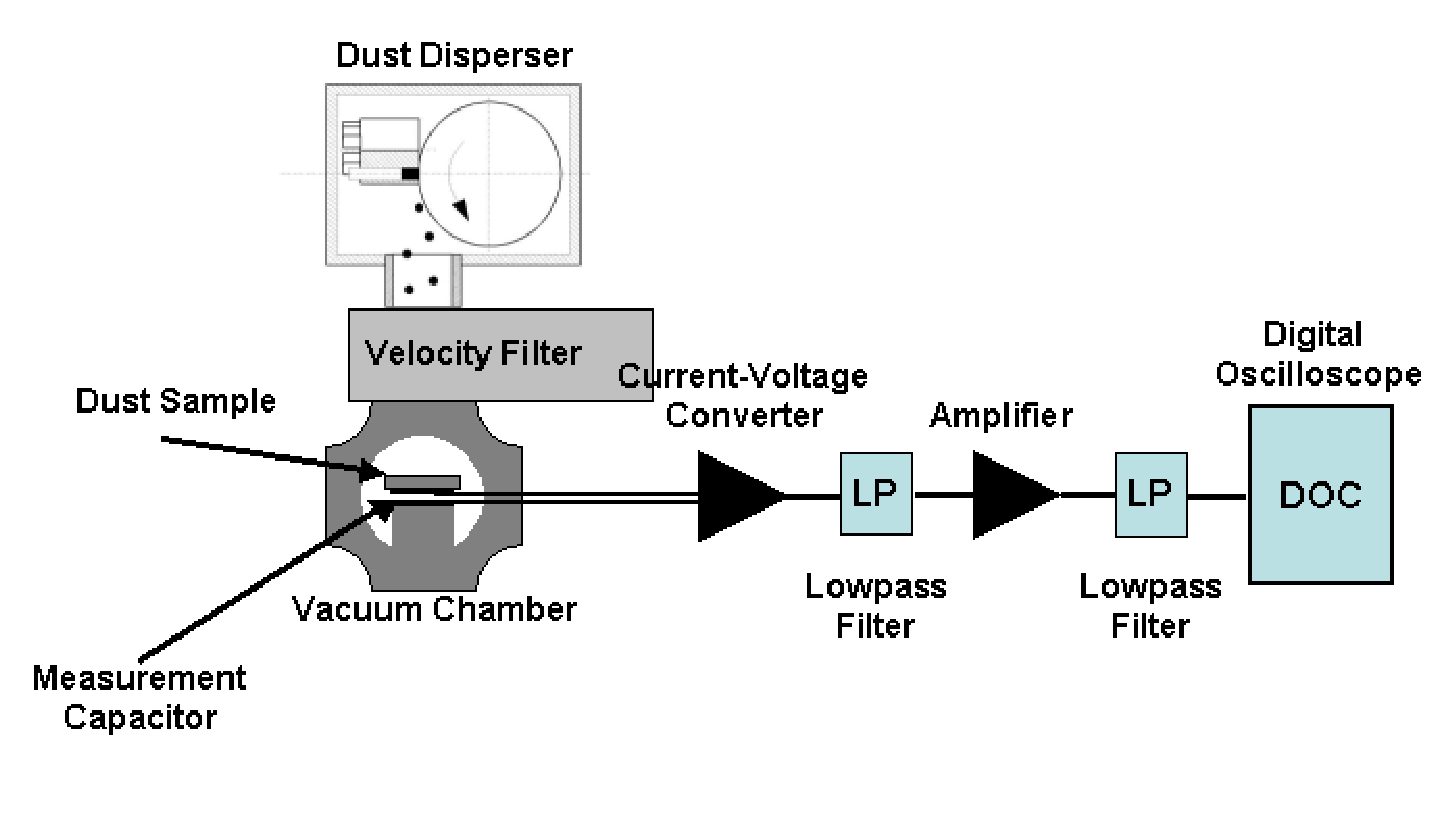
\includegraphics[width=16cm]{b1fig1.eps}}
\caption{\label{fig1blum1}Experimental setup to study the charging
of micrometer-sized dust grains in impacts with cm-sized
high-porosity dust targets.}
\end{figure}


%
% Here follows the own refereed publications by the PIs in relation to
% the project proposed here.
%
\ownpubltitle{Own publications related to the Forschergruppe:}
%
% BELOW IS ONLY AN EXAMPLE OF TWO ENTRIES. SEE THE ADDITIONAL FILES
% SENT TO YOU WITH ALL THE REFERENCES FROM THE VORANTRAG
%
\begin{ownpubl}

\item Blum, J., Wurm, G., Poppe, T. and Heim, L.-O. (1999) Aspects
of Laboratory Dust Aggregation with Relevance to the Formation of
Planetesimals. In: \textit{Laboratory Astrophysics and Space
Research}, Astrophysics and Space Science Library, Vol. 236 (Eds.
P. Ehrenfreund, K. Krafft, H. Kochan, V. Pirronello) Kluwer
Academic Publishers, Dordrecht, 399

\item Blum, J. and Wurm, G. (2000) Experiments on Sticking,
Restructuring and Fragmentation of Preplanetary Dust Aggregates.
\ica, \textbf{143}, 138-146

\item Blum, J., Wurm, G., Kempf, S., Poppe, T., Klahr, H., et al.
(2000) Growth and Form of Planetary Seedlings: Results from a
Microgravity Aggregation Experiment. \prl, \textbf{85}, 2426

\item Blum, J. and Schr\"apler, R. (2004) Structure and Mechanical
Properties of High-Porosity Macroscopic Agglomerates Formed by
Random Ballistic Deposition, \prl, \textbf{93}, 115503

\item Blum, J. (2004) Grain Growth and Coagulation, in:
\textit{Astrophysics of Dust}, ASP Conference Series, Vol. 309
(Eds. A. Witt, G. Clayton and B. Draine), 369-391

\item Heim, L.-O., Blum, J., Preuss, M. and Butt, H.-J. (1999)
Adhesion and Friction Forces Between Spherical Micrometer-Sized
Particles. \prl, \textbf{83}, 3328

\item Heim, L.-O., Butt, H.-J., Schr\"apler, R. and Blum, J.
(2005) Analyzing the Compaction of High-Porosity Microscopic
Agglomerates, Australian Journal of Chemistry, \textbf{58(9)}, 671

\item Krause, M. and Blum J., (2004) Growth and Form of Planetary
Seedlings: Results from a Sounding Rocket Microgravity Aggregation
Experiment. \prl, \textbf{93}, 021103

\item Krauss, O. and Wurm, G. (2005) Photophoresis and the Pile-up
of Dust in Young Circumstellar Disks, \apj, \textbf{630}, 1088

\item Motschmann, U., Sauer, K. and Roatsch, T. (1992) Simulation
of ion acceleration in a charged dust cloud, Geophys. Res. Lett.,
\textbf{19}, 225

\item Poppe, T., Blum, J. and Henning, Th. (1997) Generating a jet
of deagglomerated small particles in vacuum. \textit{Review of
Scientific Instruments\/}, \textbf{68}, 2529

\item Poppe, T., Blum, J. and Henning, Th. (2000a) Analogous
Experiments on the Stickiness of Micron-Sized Preplanetary Dust.
\apj, \textbf{533}, 454-471

\item Poppe, T., Blum, J. and Henning, Th. (2000b) Experiments on
Collisional Grain Charging of Micron-sized Preplanetary Dust.
\apj, \textbf{533}, 472-480

\item Poppe, T. and Schr\"apler, R. (2005) Further Experiments on
Collisional Tribocharging of Cosmic Grains. \aap, \textbf{438}, 1

\item Wurm, G. and Blum, J. (1998) Experiments on Preplanetary
Dust Aggregation. \ica, \textbf{132}, 125

\item Wurm, G., Paraskov, G. and Krauss, O. (2005a) Ejection of
Dust by Elastic Waves in Collisions between Millimeter- and
Centimeter-sized Dust Aggregates at 16.5 to 37.5 m/s Impact
Velocities. \phre, \textbf{71}, 21304

\item Wurm, G., Paraskov, G. and Krauss, O. (2005b) Growth of
Planetesimals by Impacts at ~25m/s. \ica, \textbf{178}, 253-263

\item Wurm, G. and Krauss, O. (2006) Concentration and Sorting of
Chondrules in the Late Solar Nebula. \ica, \textbf{180}, 487-495.

\end{ownpubl}
%
\section{Goals (Ziele)}
Under the conditions of the protoplanetary nebula, larger,
non-fractal dust aggregates are subject to collisions with smaller
dust particles and agglomerates. The impinging projectiles are
either embedded in the target agglomerate (mass gain) or
rebound/fragment upon impact (primary mass loss). The current
understanding is that the growth of pre-planetesimal bodies beyond
a size of $\sim 0.1$~m can no longer be governed by direct
hit-and-stick collisions. Experiments with micrometer-sized
particles have shown (Poppe et al.~2000b, Poppe \& Schr\"apler
2005) that upon impact, target and projectile are charged. A
succession of non-sticking impacts produces a net charge on the
target if there is a preferential charge sign on the projectiles
(as observed by Poppe et al.~2000b). In that case, the escaping
projectiles and/or fragments are deflected in the electrostatic
field after the collisions. If the net charging of the larger
bodies due to a succession of non-sticking impacts is sufficiently
large, escaping projectiles and/or fragments are driven back to
the target surface where they inevitably stick (secondary mass
gain). The here-proposed project will investigate the efficiency
and importance of this electrostatic growth process under
solar-nebula conditions, taking into account state-of-the-art
velocity fields between dust aggregates of different sizes (this
is an input from projects \projklahr{} and \projdul{}) and results
on the ionization state of the surrounding gas (Semenov et al.
2004). The following individual goals have been identified and
will be addressed by project \projblum{}:
\begin{itemize}

\item Determine the number of separated elementary charges as a
function of impact velocity, projectile and target mass,
projectile and target material, projectile and target porosity,
and impact angle.

\item Observation of growth and erosion as a function of impact
velocity, projectile and target mass, projectile and target
material, projectile and target porosity, and impact angle.

\item Determination of coefficients of restitution and ejecta
velocities, angles, and mass distributions.

\item Determination of the charge per ejecta particle in
fragmentation and/or cratering events.

\item Provide input for coagulation equation (i.e.\ input to
project \projdul{}).

\item Modelling of the efficiency of electrostatic secondary
agglomeration under solar nebula conditions, i.e.\ taking into
account realistic collision velocities of the dust and ionization
levels of the gas.

\item Assess the feasibility of electric discharges in the solar
nebula and their importance for chondrule formation.

\end{itemize}

As a side effect, the experiments of project \projblum{} will
result in a much better mapping of the outcomes of mutual
dust-aggregate collisions under the conditions of protoplanetary
disks. Important properties, such as sticking probabilities,
fragmentation probabilities, and fragment size distributions will
be directly available to project \projdul{} for a model refinement
of the overall growth and development towards planetesimals.


\section{Work schedule (Arbeitsprogramm)}
\subsection{Methods}
In the proposed project, impacts of $\rm \mu m$-cm dust
particles/agglomerates into dusty targets of various porosities at
velocities $1 \ldots 100$ m/s are foreseen (see Table
\ref{tab1blum1}). We will extensively make use of existing
experimental hardware in the proposing laboratories (see Sect.
Preliminary work). In the type 1 experiments, single-particle
projectiles will initially be accelerated by the cogwheel dust
disperser (Poppe et al.~1997) with adjacent velocity filter (see
Fig. \ref{fig1blum1}). Parallel to that, a disperser for neutral
dust grains will be developed. Larger dust agglomerates will be
accelerated by recently-developed techniques in the Braunschweig
(stepper motor driven accelerator for high-porosity, mm-sized
agglomerates, type 2 experiments) and M\"unster (cross-bow
accelerator for mm-cm-sized intermediate- to low-porosity
agglomerates, type 3 experiments) laboratories.

\begin{table}[h]
\caption{\label{tab1blum1}Overview of the three experiment types
to be performed in project \projblum{}.}
{\footnotesize %\hspace{-1.0cm}
\begin{tabular}{|l||l|l|l|}
  % after \\: \hline or \cline{col1-col2} \cline{col3-col4} ...
  \hline
  Method & Type 1 & Type 2 & Type 3\\
   \hline
   \hline
  Projectiles & Single micrometer-sized & high-porosity  & intermediate- to low- \\
  & dust grains of arbitrary shape & dust agglomerates & porosity dust agglomerates\\
  \hline
  Targets & low- to high-porosity & low- to high-porosity & low- to high-porosity\\
  & dust agglomerates & dust agglomerates & dust agglomerates\\
  \hline
  Impact velocities & $\sim 1 \ldots 50$~m/s & $\sim 1 \ldots 20$~m/s
  & $\sim 10 \ldots 100$~m/s\\
  \hline
  Observations of & long-distance & high-speed & high-speed \\
  projectile impact & microscopy & camera & camera \\
  \hline
  Measurement of & charge amplifier & deflection of particles &
  deflection of particles\\
  charge transfer & & in electric field & in electric field\\
  \hline
  Additional & Mass gain/loss & Mass gain/loss & Mass
  gain/loss\\
  measurements & of target agglomerate & of target agglomerate & of target
  agglomerate\\
  \hline
\end{tabular}
}
\end{table}

Observations of the impacts are performed by long-distance
microscopic imaging for single-particle type 1 impacts (Poppe et
al.~2000a), and by high-speed imaging techniques for impacting
dust aggregates (type 2 and 3). For these observations, a
high-resolution long-distance microscope (type 1), telecentric
objectives (type 2 and 3), and high-speed cameras (from 500 fps at
1,280 $\times$ 1,024 pixel to 10,000 fps at 65 $\times$ 1,024
pixel) with corresponding illuminations (flash lamps, high-power
halogen lamps, pulsed and continuum lasers) are available at the
proposing laboratories. A plate capacitor for the deflection of
charged ejecta will be used in experiments with projectile
agglomerates (type 2 and 3). This well-established technique
allows the measurements of the coefficients of restitution of
bouncing projectiles and particle trajectories for all ejecta. Due
to the electric field in which the ejecta are travelling, their
acquired charges can be calculated. We expect to be able to
observe electrostatic re-attraction of escaping particles caused
by charge accumulation on the target agglomerate. These
experiments will be extensively performed in the laboratory and
will, if required, also be run in the drop tower under
microgravity conditions. Due to the short experiment time in the
drop tower (up to 9 seconds), an artificial electrical field has
to be applied to simulate the charge accumulation on the target.
The field strength will be adapted to the results of the
long-duration laboratory experiments so that the occurrence of
electrostatic re-accretion can be observed under realistic
experimental conditions. For the experiments with impinging
individual dust particles (type 1), the recently developed
charge-measurement setup will be used (see Fig.\ \ref{fig1blum1}
and Sect.\ 5).

With these experiments, we will try to cover most of the necessary
parameter space. The experimental parameters to be investigated
comprise of (1) porosity of target agglomerate, (2) porosity of
projectile agglomerate (within the limits of the accelerators, see
Table \ref{tab1blum1}), (3) impact velocity, and (4) impact angle
(i.e.\ normal impacts and oblique impacts). Using the experimental
results, a model of the temporal evolution of surface charges of
pre-planetesimal bodies will be developed. The model will include:
\begin{enumerate}
    \item {\bf Charge transfer between projectile and the target
    agglomerate, caused by rebound, fragmentation, or cratering.}\\
    As the
    experiments in this project systematically scan the relevant
    parameter space for collision-induced grain charging, such as
    collision velocity, projectile mass, projectile and target
    material and porosity, we expect to have, at the end of the
    experimental section, a clear view on how many elementary
    charges are separated in which collision.
    \item {\bf Build-up of surface charges on the
    target agglomerate by consecutive non-sticking impacts.}\\
    In the
    second step, we will calculate a typical sequence of impacts
    into an arbitrary dust agglomerate in the protoplanetary
    nebula (this uses extensive input from project \projdul{}) and the
    corresponding accumulation of surface charges (and their
    statistical distribution over the surface), initially not taking into
    account possible discharges by nebula electrons/ions.
    \item {\bf Calculations of the resulting electrical field strength.}\\
    With the
    knowledge of the charge distribution over the surface of the
    dust agglomerate, the near-surface field strength of the
    electric field can be computed. This can be done using the
    COMSOL software package that is available in the Braunschweig
    laboratory.
    \item {\bf Statistical analysis of projectile/fragment
    trajectories within the electrical field in the vicinity of
    the target agglomerate (also taking into account aerodynamic
    drag effects).}\\
    Based upon the measurements of the ejecta
    velocity and angular distribution upon impact, we will compute
    the possible ejecta trajectories to determine the fraction of
    ejecta that are re-accreted by the pre-planetesimal. The
    result of this computation will be the efficiency of
    electrostatic capturing under the conditions of the
    protoplanetary nebula.
    \item {\bf De-charging of the agglomerates by the solar nebula
    gas.}\\
    In the final stage of the modelling effort, we will also take
    into account possible charging/discharging mechanism by the
    electrons/ions in the nebula gas. This effort will be executed
    in close collaboration with D. Semenov at the MPIA and R.
    Nelson/M. Ilgner at QMU who have extensive experience
    in modelling the charge state of the nebula gas.
\end{enumerate}

The final result of the model shall be an assessment about the
importance and efficiency of secondary electrostatic agglomeration
under protoplanetary nebula conditions and a description of the
charging effect in the coagulation equation (input to project
\projdul{}). As a side effect, it is expected that the experiments
and the model will give insight into the occurrence of large-scale
charge separation which might lead to electrostatic discharges
(lightning) in the solar nebula.


\subsection{Schedule}

\subsubsection{First year}
In the first year, the PhD student will build the necessary
hardware components for the three experimental setups described in
Table \ref{tab1blum1} and will extensively test the performance of
the setups. This construction and testing phase will comprise of
the development of a disperser for neutral particles and the
charge measurements in the type 1 experiments, the plate
capacitors and their electrical supplies for the type 2 and 3
experiments, and the observational components for all types of
experiments. In addition to that, software for the data analysis
has to be written. This encompasses trajectory detection
algorithms and the corresponding derivation of the charge-to-mass
ratios of the ejecta. Moreover, ejecta masses are required for the
determination of the charge state of the particles from their
charge-to-mass values. Algorithms for the particle-mass
determination from high-speed images therefore also need to be
developed.

\subsubsection{Second year}
In the second year, systematic laboratory measurements of charging
efficiencies in projectile-target collisions with single-grain and
aggregate projectiles as well as with targets of various
porosities will be performed (type1, type 2, and type 3
experiments). The experiments shall cover the full parameter space
in impact velocity, projectile type, target type, and particle
material. Type 1 and type 2 experiments will be performed in the
Braunschweig laboratory, type 3 experiments will be done in
M\"unster. If the results of the experiments show a considerable
influence of gravity on the results, a series of microgravity
drop-tower experiments on collision-induced grain charging will be
done. The Braunschweig and M\"unster groups have extensive
experience with short-duration microgravity experiments and will
support the development of a miniaturized and autonomous
experimental setup for the drop-tower campaign.

\subsubsection{Third year}
In the final year, a model of charging and discharging of dust
aggregates under the conditions of a protoplanetary nebula shall
be developed following the strategy outlined above. The model
steps comprise of the mapping of the charge transfer between
projectile and the target agglomerate, calculations of the
build-up of surface charges on the target agglomerates by
consecutive non-sticking impacts, computations of the resulting
electrical field strengths, a statistical analysis of
projectile/fragment trajectories within the electrical field in
the vicinity of the target agglomerates, and the de-charging of
the agglomerates by the solar nebula electrons/ions. As a final
result, we expect to compute re-capturing efficiencies of
non-sticking dust particles/aggregates and an assessment on the
importance of this effect for the formation of planetesimals. In
addition, the occurrence of large-scale charge separation will be
calculated and the probability of chondrule melting by electric
discharges will be addressed. Results of the experimental and
theoretical investigations will be published in peer-reviewed
journals.

\subsection{Literature}
%
% Here follows a general literature list related to the topic of the
% proposal, just like a literature list for a scientific paper.
%
% AGAIN ONLY EXAMPLES ARE LISTED NOW
%
\begin{literature}

\item Amelin, Y., Krot, A. N., Hutcheon, I.D. and Ulyanov, A.A. (2002) 
Lead isotopic ages of chondrules and calcium-aluminum-rich inclusions.
\textit{Science} \textbf{297}, 1678--1682.

\item Barge, P. and Sommeria, J. (1995) Did planet formation begin
inside persistent gaseous vortices?, \aap, \textbf{295}, L1

\item Blum, J., Wurm, G., Poppe, T. and Heim, L.-O. (1999) Aspects
of Laboratory Dust Aggregation with Relevance to the Formation of
Planetesimals. In: \textit{Laboratory Astrophysics and Space
Research}, Astrophysics and Space Science Library, Vol. 236 (Eds.
P. Ehrenfreund, K. Krafft, H. Kochan, V. Pirronello) Kluwer
Academic Publishers, Dordrecht, 399

\item Blum, J. and Wurm, G. (2000) Experiments on Sticking,
Restructuring and Fragmentation of Preplanetary Dust Aggregates.
\ica, \textbf{143}, 138-146

\item Blum, J., Wurm, G., Kempf, S., Poppe, T., Klahr, H., et al.
(2000) Growth and Form of Planetary Seedlings: Results from a
Microgravity Aggregation Experiment. \prl, \textbf{85}, 2426-2429

\item Blum, J. (2004) Grain Growth and Coagulation, in:
\textit{Astrophysics of Dust}, ASP Conference Series, Vol. 309
(Eds. A. Witt, G. Clayton and B. Draine), 369-391

\item Blum, J. and Schr\"apler, R. (2004) Structure and Mechanical
Properties of High-Porosity Macroscopic Agglomerates Formed by
Random Ballistic Deposition, \prl, \textbf{93}, 115503

\item Ciesla, F.~J. (2005) Chondrule-forming Processes: An
Overview. In Chondrites and the Protoplanetary Disk (A.N Krot, E.R.D.
Scott, and B. Reipurth, Editors). ASP Conference Series vol.\ 341,
Astronomical Society of the Pacific, San Francisco. pp.\
811-820.

\item Cuzzi, J.~N., Dobrovolskis, A.~R. and Champney, J.~M. (1993)
Particle-gas dynamics in the midplane of a protoplanetary nebula
\ica, \textbf{106}, 102

\item Dominik, C. and Tielens,  A.~G.~G.~M. (1997) The Physics of
Dust Coagulation and the Structure of Dust Aggregates in Space.
\ica, \textbf{480}, 647

\item Gibbard, S.G., Levy, E.H. and Morfill, G.E. (1997), On the
Possibility of Lightning in the Protosolar Nebula, \ica,
\textbf{130}, 517

\item Heim, L.-O., Blum, J., Preuss, M. and Butt, H.-J. (1999)
Adhesion and Friction Forces Between Spherical Micrometer-Sized
Particles. \prl, \textbf{83}, 3328

\item Heim, L.-O., Butt, H.-J., Schr\"apler, R. and Blum, J.
(2005) Analyzing the Compaction of High-Porosity Microscopic
Agglomerates, Australian Journal of Chemistry, \textbf{58(9)} 671

\item Johansen, A., Klahr, H. and  Henning, Th. (2006)
Gravoturbulent formation of planetesimals. \apj, (in press)

\item Krause, M. and Blum J., (2004) Growth and Form of Planetary
Seedlings: Results from a Sounding Rocket Microgravity Aggregation
Experiment. \prl, \textbf{93}, 021103

\item Krauss, O. and Wurm, G. (2005) Photophoresis and the Pile-up
of Dust in Young Circumstellar Disks. \apj, \textbf{630}, 1088

\item Morfill, G., Spruit, H. and Levy, E.H. (1993) Physical
Processes and Conditions Associated with the Formation of
Protoplanetary Disks, In: \textit{Protostars and Planets III}
(Eds. E.~H. Levy, J.~I. Lunine) University of Arizona Press,
Tucson, 939

\item Motschmann, U., Sauer, K. and Roatsch, T. (1992) Simulation
of ion acceleration in a charged dust cloud, Geophys. Res. Lett.,
\textbf{19}, 225

\item Norville, K., Baker, M. and Latham, J. (1991) A Numerical
Study of Thunderstorm Electrification: Model Development and Case
Study. {\it J. Geophys. Res.}, \textbf{96}, 7463

\item Poppe, T., Blum, J. and Henning, Th. (1997) Generating a Jet
of Deagglomerated Small Particles in Vacuum. \textit{Review of
Scientific Instruments\/}, \textbf{68}, 2529

\item Poppe, T., Blum, J. and Henning, Th. (2000a) Analogous
Experiments on the Stickiness of Micron-Sized Preplanetary Dust.
\apj, \textbf{533}, 454-471

\item Poppe, T., Blum, J. and Henning, Th. (2000b) Experiments on
Collisional Grain Charging of Micron-sized Preplanetary Dust.
\apj, \textbf{533}, 472-480

\item Poppe, T. and Schr\"apler, R. (2005) Further Experiments on
Collisional Tribocharging of Cosmic Grains. \aap, \textbf{438}, 1

\item Russell, S.S., Srinivasan, G., Huss, G.R., Wasserburg, G.J. 
and MacPherson, G.J. (1996).  Evidence for widespread $^{26}$Al in the solar
nebula and constraints for nebula time scales.  \textit{Science}
\textbf{273}, 757--762.

\item Schr\"apler, R. and Henning, Th. (2004) Dust Diffusion,
Sedimentation, and Gravitational Instabilities in Protoplanetary
Disks. \apj, \textbf{614}, 960

\item Sekiya, M. and Takeda, H. (2003) Were planetesimals formed
by dust accretion in the solar nebula? \textit{Earth, Planets and
Space\/}, \textbf{55}, 263

\item Semenov, D., Wiebe, D. and Henning, Th. (2004) Reduction of
chemical networks. II. Analysis of the fractional ionisation in
protoplanetary discs. \aap, \textbf{417}, 93

\item Wasson , J.~T. (1996) Chondrule formation: Energetics and
length scales. In: \textit{Chondrules and the protoplanetary disk}
(Eds. R.~H. Hewins, R.H. Jones, E.R.D. Scott) Cambridge University
Press, 45

\item Weidenschilling, S.~J. (1997) The Origin of Comets in the
Solar Nebula: A Unified Model \ica \textbf{127}, 290

\item Weidenschilling, S.~J. and Cuzzi, J.~N. (1993) Formation of
Planetesimals in the Solar Nebula. In: \textit{Protostars and
Planets III} (Eds. E.~H. Levy, J.~I. Lunine) University of Arizona
Press, Tucson, 1031

\item Whipple, F.L. (1966)
  Chondrules: Suggestion Concerning the Origin,
  \sci \textbf{153}, 54

\item Wurm, G. and Blum, J. (1998) Experiments on Preplanetary
Dust Aggregation. \ica, \textbf{132}, 125

\item Wurm, G., Blum, J. and Colwell, J.~E. (2001) Aerodynamical
sticking of dust aggregates. \phre, \textbf{64}, 046301

\item Wurm, G., Paraskov, G. and Krauss, O. (2004) On the
Importance of Gas Flow through Porous Bodies for the Formation of
Planetesimals. \apj, \textbf{606}, 983

\item Wurm, G., Paraskov, G. and Krauss, O. (2005a) Ejection of
dust by elastic waves in collisions between millimeter- and
centimeter-sized dust aggregates at 16.5 to 37.5 m/s impact
velocities. \phre, \textbf{71}, 21304

\item Wurm, G., Paraskov, G. and Krauss, O. (2005b) Growth of
Planetesimals by Impacts at ~25m/s. \ica, \textbf{178}, 253-263

\item Wurm, G. and Krauss, O. (2006) Concentration and Sorting of
Chondrules in the Late Solar Nebula. \ica, \textbf{180}, 487-495.
\end{literature}



\section{External/International collaborations}
\begin{collablist}


\item[MPIA Heidelberg] Dr. D. Semenov will use the results from
this project for revised calculations on the ionization levels and
chemical processes in protoplanetary disks. In addition to that,
Dr. Semenov will model the timescales of charging/discharging of
solid bodies due to electron/ion fluxes in protoplanetary disks to
help assess the importance of electrostatic re-accretion.

\item[Nagoya Univ.] Dr. S. Sirono will use the results of the
impact studies for his mechanical and structural model of
protoplanetary dust aggregates.

\item[Queen Mary Univ. of London] Prof. Dr. R. Nelson, Dr. M.
Ilgner will use the results of this work for their studies on
solar-nebula chemistry and can give valuable input on discharging
timescales.

\end{collablist}



\section{Link to other projects of the Forschergruppe}
\begin{linkproj}

\item[\projtscharn{},\projlattard{}] Projects \projtscharn{} and
\projlattard{} will provide input on abundances of various
minerals to be expected at various parts of the disk. Due to the
detailed chemical and mineralogical modelling in projects
\projtscharn{} and \projlattard{}, much better constraints on the
abundances of the minerals will be available to project
\projblum{}. Thus, the laboratory experiments in project
\projblum{} can always be carried out with dust particles produced
under state-of-the-art knowledge on their relevance.

\item[\projwurm{}] A strong interaction with project \projwurm{}
is envisioned because of common experimental hardware. Both
projects will use identical setups and hardware components so that
a concerted experimentation is required from the logistic as well
as from the scientific point of view. Results of either
experiments can (and possibly will) influence the proceedings of
the respective other work so that a strong interaction between
projects \projwurm{} and \projblum{} is required and foreseen.

\item[B3] Will use experience gained in B3
in using realistic materials such as Mg, Ca, Al silicates and/or Fe-Ni metal
for the planned coagulation experiments.

\item[\projkley{}] The results from the experiments  will provide
input parameters for the SPH code in project \projkley{}, such as
%sticking probabilities and fragmentation outcomes in
%aggregate-aggregate collisions. 
sound speed and elasticity of the porous material.
High-speed, high-resolution
imaging, as used in project \projblum{}, can also help to reveal
the dynamical behavior of interacting dust agglomerates and can be
used to calibrate the SPH simulations.

\item[\projklahr{}] Project \projklahr{} will yield typical impact
velocities for certain aggregate sizes and aggregate properties so
that any findings of project \projklahr{} will influence the
parameter space to be covered in project \projblum{}. On the other
hand results from this project can also influence the modelling in
project \projklahr{} if, under the conditions investigated there,
impact charging plays an important role.

\item[\projdul{}] The experiments in project \projblum{} will
provide valuable input parameters for the dust-dust interactions
for project \projdul{} and will help to define correction terms
for the reaction and coagulation kernel in Smoluchowski's equation
which is the basis for project \projdul{}. Vice versa, project
\projdul{} will be able to predict aggregate abundances, collision
probabilities and collision velocities in protoplanetary disks,
which all are important input parameters for the experiments in
project \projblum{}. As part of the project, an extensive
iteration between laboratory work and modelling efforts is
envisioned.

\item[D1] The textures of agglomerates coagulated under various conditions 
can be directly compared with fine-grained, primitive chondrite assemblages
and cometary dust particles analysed with transmission electron microscopy
/SEM / TOF-SIMS/Nano-SIMS in D1.

\end{linkproj}



\section{\label{persb1}Team members (Zusammensetzung der Arbeitsgruppe)}
%
% NOTE: Only list non-DFG-funded team members.
% NOTE: Also list technical assistants, students etc involved in the project
%
\begin{teamlist}

\item[Blum, J., Prof.~Dr. (C3)]\mbox{}\\
Team leader. Overlooks the experimental and modelling efforts and
supervises the PhD student funded through this project. Provides
extensive expertise in dust collisions, high-speed imaging
techniques, and microgravity experimentation.

\item[Wurm, G., Dr.]\mbox{}\\
Team co-leader. Hosts the PhD student for the type 3 experiments
and for regular visits in M\"unster. Provides extensive expertise
in high-velocity dust impacts and microgravity experimentation.

\item[Kley, W., ~Prof.~Dr. (C4)]\mbox{}\\
Team collaborator. Leads project \projkley{} in which an SPH code
on aggregate-aggregate collisions will be developed. Strong
interactions between \projkley{} and \projblum{} is foreseen to
enhance the output and relevance of both projects.

\item[Motschmann, U., Prof.~Dr. (C3)]\mbox{}\\
Team collaborator. Has widespread experience in modelling
electromagnetic fields and plasmas and will assist in the
development of the theoretical model.

\item[Dullemond, C.P., Dr.]\mbox{}\\
Team collaborator. Is responsible for the transfer of the results
of project \projblum{} to the coagulation code to be developed in
project \projdul{}. Vice versa, valuable input on
aggregate-aggregate collision velocities and frequencies for
project \projblum{} will be provided by \projdul{}.

\item[Klahr, H., Dr.]\mbox{}\\
Team collaborator. Is responsible for the transfer of the results
of project \projklahr{} on aggregate-aggregate collision
velocities and frequencies to project \projblum{}.

\item[Poppe, T., Dr.]\mbox{}\\
Internal collaborator. Dr. Poppe lead the earlier work on impact
charging and will assist the project.

\item[Schr\"apler, R., Dr.]\mbox{}\\
Internal collaborator. Has led the development of the experimental
setup for the type 1 experiments; has extensive experience in
charge measurements and the acceleration and control of
microscopic particles.

\item[Krau{\ss}, O., Dr.]\mbox{}\\
Internal collaborator. Dr. Krau{\ss} has extensive experience in
dust-impact research in the laboratory and in the drop tower.

\item[Stoll, B.]\mbox{}\\
Electronics Engineer. Will assist in the experimental setups on
charge measurements.

\item[Jelting, E.]\mbox{}\\
Electronics Engineer. Will assist in the experimental setups on
charge measurements.

\item[Gebauer, K.]\mbox{}\\
Mechanics Technician. Will assist in the construction of new
experimental hardware.


\end{teamlist}
\vspace{1em}



\section{Funding requested}
The following table gives the full overview of requested
funding:\vspace{1\baselineskip}\\
%
% The table that follows is the overview over the full requested
% funding, including the positions, travel, consumables and ``other
% costs'' (which might include transportation costs of radioactive
% material or the rent of a drop tower or such).
%

\centerline{
\begin{tabular}{||l|l|l|l||} \hline \hline & Year 1 & Year 2 &
Year 3 \\ \hline %
Personnel (1 PhD-students: E13/2)   & \hfill 24,000  & \hfill 24,000 & \hfill 24,000 \\
Equipment                           & \hfill 12,269  & \hfill -      & \hfill - \\
Consumables                         & \hfill 9,000   & \hfill 7,000  & \hfill 6,000 \\
Travel                              & \hfill 4,000   & \hfill 5,600  & \hfill 5,600 \\
Other costs                         & \hfill -       & \hfill  -     & \hfill  -    \\
\hline
{\bf Total:}                        & \hfill 49,269 & \hfill 36,600 & \hfill 35,600 \\
\hline \hline
\end{tabular}
}

\vspace{1em}

{\noindent Below these costs are explained in more detail:}

\subsection{Personnel (Personalbedarf)}
\begin{teamlist}
\item[PhD-Student (E13/2)]\mbox{}\\
The PhD student shall perform independent experimental and
theoretical research to reveal the importance and efficiency of
electrostatic agglomeration.
\end{teamlist}

\subsection{Equipment (Ger\"ate)}

For the experiments to be performed within project \projblum{},
high-vacuum equipment is mandatory. Due to possible electrical
discharges, a mechanical pump is not sufficient, but needs to be
augmented by a turbo-molecular pump. A complete setup is available
from Leybold (PT 50) at a cost of EUR 7,923. A dedicated vacuum
chamber, consisting of a CF-100 double-cross-piece (EUR 1,699 at
Leybold) and 6 CF-100 flanges (EUR 647 at Leybold), will be
purchased for the housing of the experiment. Vacuum gauges are
available at the Braunschweig laboratory at no cost. A
work-station PC with image analysis software for the PhD student
is required. The cost of this PC will be approximately EUR 2,000.

Estimated cost:\vspace{1\baselineskip}\\
\centerline{
\begin{tabular}{||l|l|l|l||} \hline \hline & Year 1 & Year 2 &
Year 3 \\ \hline %
High-vacuum pump &  \hfill 7,923 & \hfill - & \hfill - \\
Vacuum chamber & \hfill 2,346 & \hfill -& \hfill -\\
PC &  \hfill 2,000 & \hfill - & \hfill - \\
\hline
{\bf Total:}    & \hfill 12,269 & \hfill - & \hfill - \\
\hline \hline
\end{tabular}
}


\subsection{Consumables (Verbrauchsmaterial)}
The experiments require rather large amounts of dust. As some
experiments shall be used for calibration purposes of the SPH code
(project \projkley{}) and linking to earlier works, they will
consume spherical, mono-disperse, micrometer-sized $\rm SiO_2$
particles. We estimate the annual cost for this dust to EUR 1,500
(corresponding to 100 g). Other dust types are somewhat cheaper
but will be consumed in higher quantities so that an additional
estimated EUR 4,500 will be required. For the connection of the
high-vacuum pump to the experiment chamber, vacuum components
(flanges etc.) are required which will cost EUR 2,000 (in year 1
only). For the development of a disperser for neutral dust
particles in the type 1 experiments, workshop material (metals,
tools) is required in year 1 and year 2. We estimate the annual
costs to be EUR 1,000.

Estimated cost:\vspace{1\baselineskip}\\
\centerline{
\begin{tabular}{||l|l|l|l||} \hline \hline & Year 1 & Year 2 &
Year 3 \\ \hline %
Dust particles &  \hfill 6,000 & \hfill 6,000 & \hfill 6,000 \\
Vacuum equipment& \hfill 2,000 & \hfill -& \hfill -\\
Workshop material&\hfill 1,000 & \hfill 1,000 & \hfill -\\
\hline
{\bf Total:}    & \hfill 9,000 & \hfill 7,000 & \hfill 6,000 \\
\hline \hline
\end{tabular}
}

\subsection{Travel expenses in addition to Project Z (Reisekosten)}
%
% Here only travel expenses not related to usual regular Forschergruppe
% meetings and the overall per capita budget for conferences.
%
Regular project meetings with the participants of this projects
are required. We estimate that two full-day meetings per year (at
various locations) are required. For each person, the cost per
meeting will be EUR 150 for the train, EUR 50 for hotel and EUR 50
for per diem, i.e.\ a total of EUR 250. For each meeting, the
number of travellers is estimated to be three so that a total of
EUR 750 is required. In addition to that, two regular one-week
preparation visits per year by the PhD student to M\"unster (year
1, year 2) and Heidelberg/T\"ubingen (year 3) are required. Each
trip will cost EUR 150 (train) + EUR 100 (per diem) + EUR 200
(hotel) = EUR 450. Additionally, the PhD student is required to
make extensive (three-week) measurement campaigns in M\"unster.
Each campaign will cost EUR 200 (rental car) + EUR 500 (per diem)
+ EUR 900 (hotel) = EUR 1,600. A drop tower campaign demands a
three-week presence in Bremen; thus, the costs will be equivalent
to that of the other three-week campaigns (EUR 1,600). Two
drop-tower campaigns (years 2,3) are foreseen.

Estimated cost:\vspace{1\baselineskip}\\
\centerline{
\begin{tabular}{||l|l|l|l||} \hline \hline & Year 1 & Year 2 &
Year 3 \\ \hline %
Regular meetings &  \hfill 1,500 & \hfill 1,500 & \hfill 1,500 \\
Preparation visits& \hfill 900 & \hfill 900 & \hfill 900 \\
Measurement campaign & \hfill 1,600 & \hfill 1,600 & \hfill 1,600 \\
Drop-tower campaign & \hfill - & \hfill 1,600 & \hfill 1,600 \\
\hline
{\bf Total:}    & \hfill 4,000 & \hfill 5,600 & \hfill 5,600 \\
\hline \hline
\end{tabular}
}

\subsection{Other costs (Sonstige Kosten)}
There are no others costs.
%%Publication costs will amount to EUR 1,000 for the years 2 and 3.

%Estimated cost per year:\vspace{1\baselineskip}\\
%\centerline{\begin{tabular}{|p{15em}|p{10em}|p{7em}|}
%\hline
%?  & \hfill ? & \hfill ? \\
%\hline
%\end{tabular}}

%Estimated cost:\vspace{1\baselineskip}\\
%\centerline{
%\begin{tabular}{||l|l|l|l||} \hline \hline & Year 1 & Year 2 &
%Year 3 \\ \hline %
%Publication costs & \hfill - & \hfill 1,000 & \hfill 1,000 \\
%\hline
%{\bf Total:}    & \hfill - & \hfill 1,000 & \hfill 1,000 \\
%\hline \hline
%\end{tabular}
%}


\section{Preconditions for carrying out the project at home institution}
%
% This is one of the main subsections of a DFG Normalverfaren proposal.
% Several of the subsubsections in this subsection we have placed in their
% own subsections above (like team members, collaborations). What remains
% are the following three subsections. For those not familiar with these,
% we refer to the DFG Merkblatt on Normalverfahren-proposals.
%
\subsection{\label{equipb1}Scientific equipment available (Apparative Ausstattung)}
%
% Please list those larger instruments available to you for the project (if
% applicable also larger computer equipment in case you need substantial
% amounts of computer time).
%
In the Braunschweig and M\"unster laboratories, the following
equipment is available for this project at no cost:
\begin{itemize}

\item High-speed, high-resolution camera Mikrotron 1310, from 500
frames per second at 1,280 $\times$ 1,024 pixel to 10,000 frames
per second at 65 $\times$ 1,024 pixel for the type 1-3 laboratory
experiments.

\item Ruggedized high-speed, high-resolution camera Vossk\"uhler
HCC, from 462 frames per second at 1,024 $\times$ 1,024 pixel to
1,386 frames per second at 256 $\times$ 1,024 pixel for drop-tower
experiments.

\item Long-distance microscope with 80 mm working distance and
$\sim 1~\rm \mu m$ resolution for the type 1 experiments.

\item Telecentric objective lenses for the type 2 and type 3
experiments.

\item High-speed flash lamps (up to 1,000 per second) with
ultrashort ($\sim 1~\rm \mu s$) flash duration for type 1-3
experiments.

\item Continuous and pulsed laser diode for type 1 experiments.

\item Halogen lamps for type 2-3 experiments.

\item High-sensitivity charge measurement equipment (under
construction), comprising of charge amplifier and data recorder
for type 1 experiments.

\item High-voltage power supply for type 2-3 experiments.

\item Cogwheel-type dust deagglomerator and accelerator (up to
$\sim 50$ m/s) for preliminary type 1 experiments.

\item Velocity filter for the precipitation of unwanted particle
sizes and velocities in type 1 experiments.

\item Stepper motor driven accelerator (under construction) for
high-porosity dust aggregates and velocities up to $\sim 20$ m/s
(type 2 experiments).

\item Cross-bow accelerator for low- to medium-porosity dust
aggregates and velocities up to $\sim 100$ m/s (type 3
experiments).

\item High-precision balance (Sartorius MC 210 P; measurement
sensitivity $10^{-5}$~g at 200~g maximum mass) for target mass
determination.

\item COMSOL Multiphysics software with Earth Science Module and
Electromagnetics Module for the modelling of (1) the deflecting
electric fields for the charge measurements and of (2) the
electric fields around protoplanetesimals.

\item Vacuum gauges for high- and low-vacuum conditions.

\item Additional flash lamps, scales, and equipment to run type 3
experiments in M\"unster.

\end{itemize}


\subsection{Institution's general contribution (Laufende Mittel f\"ur Sachausgaben)}

Besides the scientific instrumentation (see Sect. \ref{equipb1})
and personnel costs (see Sect. \ref{persb1}), the proposing
institutions will support this project with EUR 1,000.

%
% Please state the annual fund for consumables which comes from the
% institution's budget or any other third party  (please list separately) to
% pay for the research for which your project is part of.  Use estimates where
% applicable.
%

%We estimate that the running costs per year of our equipment
%are:\vspace{1\baselineskip}\\
%%
%\centerline{\begin{tabular}{|p{18em}|p{7em}|p{7em}|}
%\hline
%?                & \hfil ? & \hfil ? \\
%\hline
%?                & \hfil ? & \hfil ? \\
%\hline
%\end{tabular}}




\cleardoublepage

\setcounter{equation}{0}
\setcounter{figure}{0}
%----------------------------------------------------------------------
%                        PROJECT DEFINITION
%----------------------------------------------------------------------
\renewcommand{\projnr}{B2}
\renewcommand{\projtitleshort}{Influence of multiple collisions}
\renewcommand{\projauth}{Wurm, Blum}
%
\setcounter{section}{0}
\noindent{\normalfont\sffamily\Large\bfseries Project \projnr: \projtitleshort}
%
\section{Full title:}
\hspace{1\baselineskip}\\
\centerline{\large ``The influence of multiple collisions on the evolution of dusty bodies''}
%\centerline{\large and the efficiency of electrostatic secondary agglomeration''}
%
\section{General information}\mbox{}
\subsection{Principle investigators:}
\hspace{-\baselineskip}\\\noindent
%
{\bfseries\itshape Wurm}, Gerhard, Dr.\\
Emmy Noether Reserach group, non-tenure\\
Date-of-birth: 05. April 1967, Nationality: German\\
DFG Code number of latest application: WU 321/2-4\\
Institut f\"ur Planetologie\\
Wilhelm-Klemm-Str.~10\\
48149 M\"unster\\
Tel: 0251 8339052\\
Fax: 0251 8336301\\
E-mail: gwurm@uni-muenster.de\\
Private address: Kesslerweg 50d, 48155 M\"unster, Tel: 0251 6279418\\
%
\vspace{1em}\\\noindent
{\bfseries\itshape Blum}, J\"urgen, Prof.~Dr.\\
C3, tenure\\
Date-of-birth: 05. April 1962, Nationality: German\\
DFG Code number of latest application: Bl 298-6/2\\
Institut f\"ur Geophysik und extraterrestrische Physik\\
Mendelssohnstr.~3\\
38106 Braunschweig\\
Tel: 0531 391 5217\\
Fax: 0531 391 8126\\
Email: j.blum@tu-bs.de\\
Private address: Wendenring 14, 38114 Braunschweig, Tel: 0531 1216432\\

\subsection{Co-investigators within this Forschergruppe:}
\begin{coilist}
\item O.~Krau{\ss} (IFP, Univ. M\"unster)
\item W.~Kley (TAT/CPT, Univ. T\"ubingen)
\item H.~Klahr (MPIA, Heidelberg)
\end{coilist}


\newpage

\section{Summary (Zusammenfassung)}
\subsubsection{Summary:}
The experimental data on the outcome of individual collisions with respect to planetesimal formation
is steadily growing. However, all the
work done so far assumes a certain simple initial state of two colliding bodies based on
more or less plausible assumptions. It is unknown how a target evolves over a
large number of collisions. Therefore, this project aims at understanding the self-consistent evolution
of an individual large dusty body under the influence of multiple impacts. The
role of compaction, loosening, fragmentation, elastic waves, ejection and
re-accretion of material will be studied. The project uses impact
experiments, models for individual collisions, and numerical calculations of
gas flow through porous bodies for re-accretion of fragments.

\subsubsection{Zusammenfassung:}
Die experimentelle Untersuchungen von St\"o{\ss}en einzelner K\"orper liefert stetig neue Daten \"uber den Ausgang 
von Kollisionen im Hinblick auf Planetesimalbildung. Bislang werden die Anfangsbedingungen
f\"ur die Struktur der sto{\ss}enden K\"orper allerdings
vor\-ge\-geben. Es ist derzeit nicht klar, wie sich ein K\"orper \"uber eine Vielzahl von St\"o{\ss}en hinweg
selbstkonsistent entwickelt. Ziel des Projekts ist es daher, die selbstkonsistente Entwicklung eines
K\"orpers unter
dem Einflu{\ss} sukzessiver Impakte zu verstehen. Hierbei werden die Bedeutung von Kompaktierung,
Auflockerung, Fragmentation, elastischen Wellen wie auch der Auswurf von Ejekta und die
Reakkretierung von Material untersucht. Es werden sowohl Experimente als auch
numerische Rechnungen verwendet. Letztere beinhalten die Simulation von St\"o{\ss}en und die numerische
Behandlung m\"oglicher
Reakkretion von Fragmenten durch Gasfluss durch einen por\"osen K\"orper.

\section{State of the art (Stand der Forschung)}

It is widely assumed that km-size planetesimals form by successive
collisions of smaller bodies in protoplanetary disks (Weidenschilling \&
Cuzzi~1993).  During planetesimal formation it is inevitable that
high-velocity collisions ($>50$ m/s) take place, in which small bodies ($<
10$ cm) collide with larger ones ($> 10$ cm) (Weidenschilling \&
Cuzzi~1993; Sekiya \& Takeda~2003). Early experimental work on impacts
into regolith was done by Hartmann ~(1978).  In ground based experiments a
solid impactor buried itself into the target regolith. This was initially
taken as evidence that large dusty bodies will stick in high speed
collisions at several tens of m/s. Colwell \& Taylor ~(1999) and Colwell
~(2003) revealed in microgravity experiments that an impactor rather bounces
off and that burial of the projectile was due to gravity, which masked the
rebound in the earlier ground based experiments by Hartmann ~(1978).  The
experiments by Colwell (2003) showed that only slow collisions below 20 cm/s
resulted in sticking of the solid projectile. Collisions with ice particles
by Bridges et al.~(1996) also suggested that no sticking of icy particles
would occur above a few cm/s collision velocity. Further evidence that
collisions at velocities above a few m/s are non-constructive came from
experiments on organic matter by Kouchi et al.~(2002). Even though the
material was rather sticky, no sticking of mm-size particles could be
observed above 5m/s collision velocity.  Only recently experiments showed
that high-velocity collisions can lead to mass gain if both colliding
particles are compact dust aggregates (Wurm et al.~2005b). In fact high
collision velocities might prove better for growth than medium velocity
collisions. Thus there might be different velocity regimes in which
collisions can lead to sticking or fragmentation and the details depend on
other parameters of the colliding bodies like size, porosity, material. In
summary the question which is the outcome of an individual collision depends
strongly on the morphology of the colliding bodies.  Therefore, the
morphological evolution of a larger body has strong relevance to the
question if -- and how -- planetesimals form by aggregation of smaller
bodies. This is sketched in figure \ref{Schema}.

\begin{figure}
%\centerline{\includegraphics[width=15cm]{sketch.eps}}
\centerline{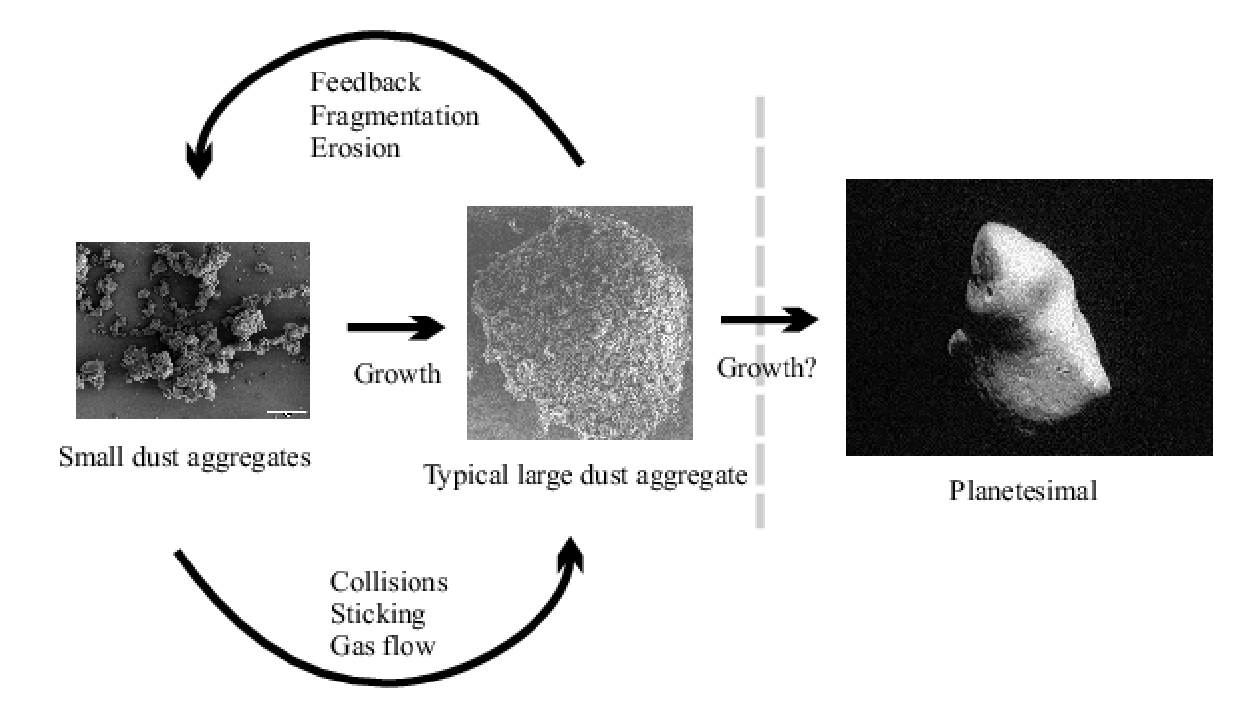
\includegraphics[width=15cm]{b2fig1.eps}}
\caption{\label{Schema}The central role of large dust aggregates of 
dm to m-size. If collisions with smaller particles on average can lead to
further growth, planetesimals might form. If collisions are disruptive in
most cases, planetesimal growth would be inhibited. In that case the typical
large aggregate would still dominate the (observable) dust distribution by
feeding smaller dust aggregates back to the disk.}
\end{figure}


Here, in a first step 'large' refers to dm to m-size bodies, since these
will collide most frequently with smaller dust aggregates due to the high
relative velocities and presumably play a dominant role in the circle of
dust recycling by growth and fragmentation. While for well-defined
parameters individual impacts have been and are simulated in the laboratory,
no self-consistent prediction of the evolution of dusty bodies has been made
yet. Numerical calculations on the evolution of the size distribution of an
evolving system of colliding particles have been carried out
(Weidenschilling 1997; Dullemond \& Dominik 2005).  These calculations
are -- so far -- based on ad hoc assumptions of sticking or fragmentation.
However, as multiple impacts occur they will gradually alter the shape and
structure (e.g.~compactness, surface, inner pore sizes) of a target body and
the outcome of the n-th collision of an evolving body is unknown and ad hoc
assumptions are currently the only way to proceed with calculations. It is
thus of fundamental importance to get a better restriction on how a growing
body evolves in morphology.

Static compression of dust aggregates leads to their compaction (Blum \&
Schr\"apler 2004b).  This does not necessarily mean that a collision will
also lead to a compaction of the colliding dust aggregates. It is found in
granular media research that local pressure can lead to a density decrease
on a larger scale. This is known as Reynolds principle of dilatancy
(Reynolds 1885).  It is also possible that a dusty body is only compacted
locally by an impact but gets decompacted on a larger scale. This has
recently been observed in drop tower experiments (Krauss et al.\ unpublished
data). In collisions onto porous target bodies, elastic waves can also eject
particles (Wurm et al.~2005a) which might be re-accreted by gas flow (Wurm et
al.~2001, 2004; Sekiya \& Takeda 2003). Such a gas flow (head wind) of up to
about 50m/s is always present for large objects due to the different motion
between the gas (sub-Keplerian) and the solids, for both cases of laminar
and turbulent disk flow (Weidenschilling 1993; Sekiya \& Takeda 2003;
Klahr et al.~2006).  The interaction of particle ejecta and gas flow is
further linked to the question on gas flow {\it through} the body which for
large porosities can be significant. It can help re-accrete small ejected
particles more efficiently if not at all (Wurm et al.~2004).  Growth and
erosion of a primary impact depend on the morphology of the colliding
bodies.  The gas flow through a body also depends on the morphology, so
morphology is one of the most important parameters. The amount of gas which
flows through the pores strongly depends on the typical pore size.
According to Darcy's law the flow velocity $q$ through a porous body is
given as

\begin{equation}
q=-\frac{k}{\mu} \frac{dp}{dx}
\end{equation}

\noindent which depends on the pressure gradient, the gas viscosity $\mu$
and the permeability $k$. The latter is proportional to the pore size
squared (Koponen et al.~1997; Cancelliere et al.~1990). Even if the
overall porosities for two bodies are equal, the difference between $\rm \mu
m$-size pores or mm-size pores can decide between (positive) re-accretion of
particles by gas flow or (negative) transport of ejecta away from an impact
side (Wurm et al.~2004; Sekiya \& Takeda 2005).

If erosion governs growth from a certain size on there will be a maximum
size target at which a typical collision will neither add nor remove mass
and growth gets stalled. The shapes and structures of these bodies then
determine which type -- and how many -- debris particles will be created
upon further collisions. This can have a profound influence on the evolution
of the size distribution of solid bodies in protoplanetary disks.
Therefore, a systematic study of the evolving structure of a growing body is
of utmost importance. The evolution upon collisions should be studied in
detail.

\section{Preliminary work (Eigene Vorarbeiten)}

Over the last decade a number of experiments and calculations have been
carried out in the laboratories in Jena, M\"unster, Boulder, and
Braunschweig to gain a better understanding of individual dust
collisions. These range from individual dust grain collisions by Poppe et
al.~(2000a) over collisions for fractal dust aggregates by Wurm \& Blum
(1998) and Blum \& Wurm (2000) to collisions of larger non-fractal but
porous dust aggregates by Langkowski \& Blum (unpublished data) and Wurm et
al.~(2005a,b) and Krauss et al.~(unpublished data). These experiments showed
that:

\begin{itemize}

\item Dust particles stick as long as they collide slower than about 1m/s.

\item Small fractal dust aggregates get fragmented at collisions faster 
  than 1m/s.

\item Fractal aggregates get compacted at about mm to cm size under 
  typical conditions in protoplanetary disks.

\item Large porous aggregates can grow in collisions with mm-size highly 
  porous projectiles at velocities up to at least 3m/s. This leads to local
  compaction.

\item Large porous aggregates can lose mass if they collide at
  several tens of m/s with a 1cm dust projectile.

\item Large porous aggregates can -- on the other side -- also
  grow in collisions with a few ten m/s if the surface is slightly
  compacted.

\item Large porous aggregates can globally get de-compacted at high 
  collision velocities.

\item Large compact aggregates can grow in high speed collisions 
  but do not grow in collisions {\bf below} about 10m/s.

\item Growth is accompanied by part of the projectile being dispersed 
  to dust particles again.

\end{itemize}

As can be seen these are a number of different outcomes which cannot be
unified in a simple picture of collisions. Therefore the more complex
approach of the research group proposed here is needed.

In a broader sense a collision might comprise secondary collisions of the
fragments ejected during a primary impact. This was found by Wurm et
al.~(2001, 2004) who showed that gas drag can lead to a re-accretion of dust
particles. A further re-accretion mechanism due to electrical charging is
proposed in project \projblum{} and will also influence the mass balance and
surface structure of an evolving dusty object.

\begin{figure}
%\centerline{\includegraphics[width=10cm]{impacts.eps}}
\centerline{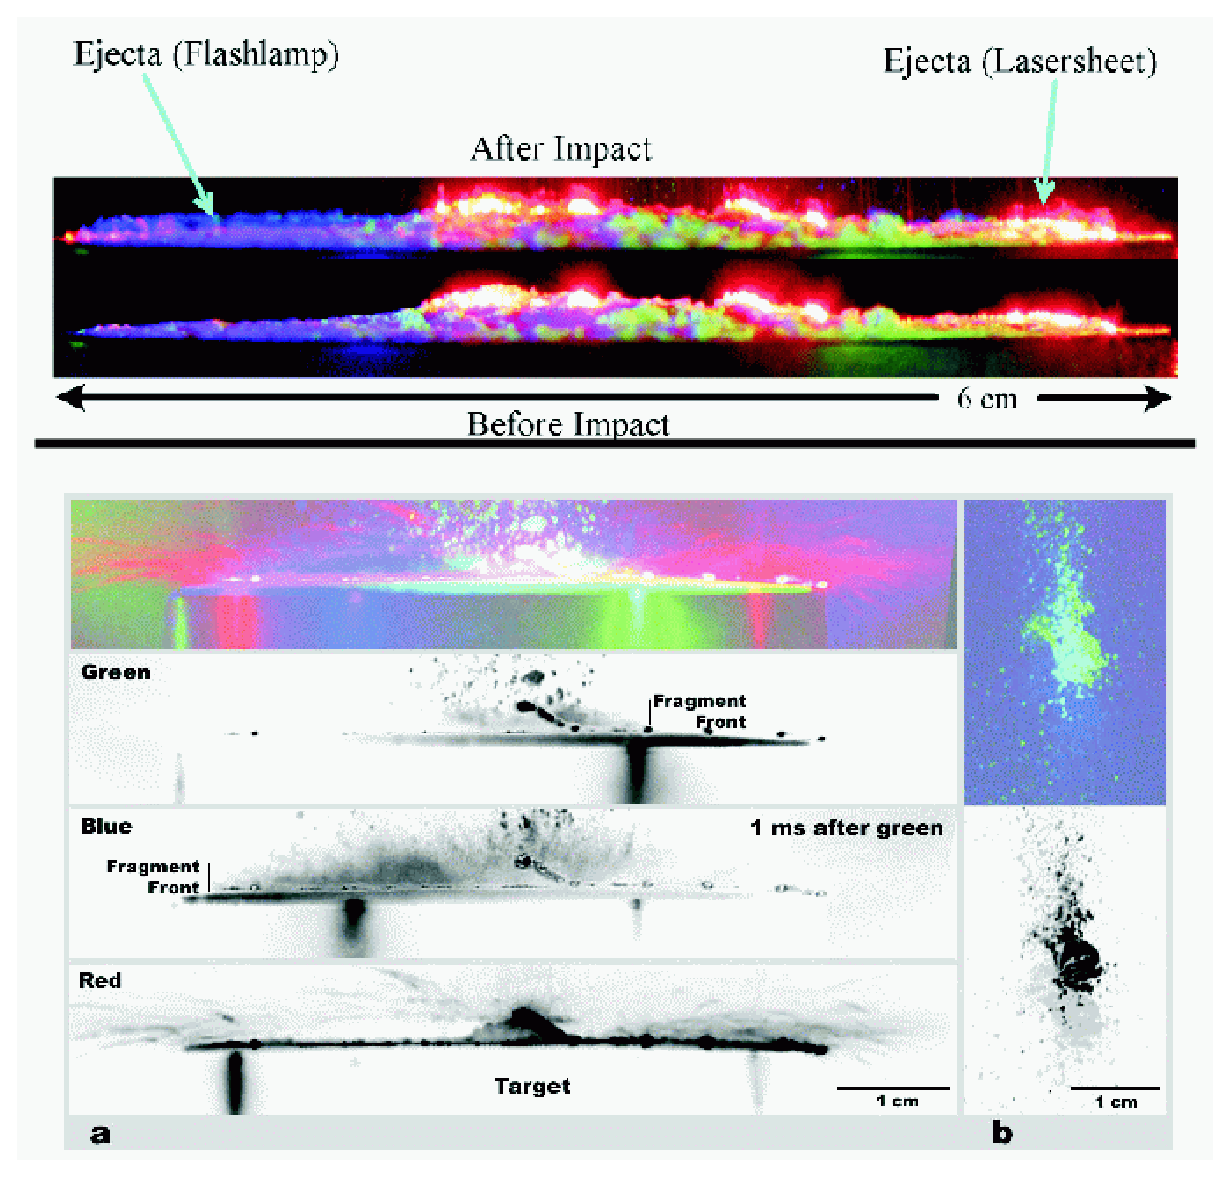
\includegraphics[width=15cm]{b2fig2.eps}}
\caption{\label{soorso}Outcome of a collision at $\rm >20m/s$. 
In the first (upper) case the collision is very destructive (Wurm et
al.~2005a). In the second (lower) case net growth occurred (Wurm et
al.~2005b).  The only difference is the initial structure of the target.}
\end{figure}


So far nearly ideal conditions have been assumed for
collisions. Experimental studies and models were mostly aiming at the
question whether a collision can lead to growth at all. Only for the
initial stage of particle growth it has been shown that the particles grow
as cluster-cluster aggregates in a self-consistent way (Blum 2004). For
larger dust aggregates, as seen in figure \ref{soorso} the outcome of a
collision, i.e.\ growth or fragmentation, strongly depends on the history of
collisions for a given target later on. While constructive and destructive
collisions have been shown to exist, it remains unclear if one of these
types of collisions is typically determining the outcome of collisions of
larger bodies with smaller ones.




%
% Here follows the own refereed publications by the PIs in relation to
% the project proposed here.
%
\ownpubltitle{Own publications related to the Forschergruppe:}
%
% BELOW IS ONLY AN EXAMPLE OF TWO ENTRIES. SEE THE ADDITIONAL FILES
% SENT TO YOU WITH ALL THE REFERENCES FROM THE VORANTRAG
%
\begin{ownpubl}
\item Blum, J. and Schr\"apler, R. (2004) Structure and Mechanical Properties of
High-Porosity Macroscopic Agglomerates Formed by Random Ballistic Deposition,
\prl, \textbf{93}, 115503

\item Blum, J. (2004) Grain Growth and Coagulation, in: \textit{Astrophysics of Dust},
ASP Conference Series, Vol. 309 (Eds. A. Witt, G. Clayton and B. Draine),
369-391

\item Blum, J. and Wurm, G. (2000) Experiments on Sticking,
Restructuring and Fragmentation of Preplanetary Dust Aggregates.
\ica, \textbf{143}, 138-146

\item Blum, J., Wurm, G., Kempf, S., Poppe, T., Klahr, H., et al.
(2000) Growth and Form of Planetary Seedlings: Results from a
Microgravity Aggregation Experiment. \prl, \textbf{85}, 2426-2429

\item Dominik, C., Blum, J., Cuzzi, J.N., Wurm, G. (2006) Growth of Dust
as the Initial Step Toward Planet Formation. in: \textit{Protostars 
and Planets V}, (Eds. B. Reipurth, D. Jewitt, K. Keil).\\ 
  {\tt http://ifa.hawaii.edu/UHNAI/ppv.htm}

\item Heim, L.-O., Butt, H.-J., Schr\"apler, R. and Blum, J.
(2005) Analyzing the Compaction of High-Porosity Microscopic
Agglomerates, Australian Journal of Chemistry, \textbf{58(9)} 671

\item Paraskov, G.B., Wurm, G., and Krauss, O. (2006) Eolian Erosion of
Dusty Bodies in Protoplanetary Disks. \apj, (accepted)

\item Poppe, T., Blum, J. and Henning, Th. (2000) Analogous
Experiments on the Stickiness of Micron-Sized Preplanetary Dust.
\apj, \textbf{533}, 454-471

\item Wurm, G., Paraskov, G. and Krauss, O. (2005) Ejection of
Dust by Elastic Waves in Collisions between Millimeter- and
Centimeter-sized Dust Aggregates at 16.5 to 37.5 m/s Impact
Velocities. \phre, \textbf{71}, 21304

\item Wurm, G., Paraskov, G. and Krauss, O. (2005) Growth of
Planetesimals by Impacts at ~25m/s. \ica, \textbf{178}, 253-263

\item Wurm, G. and Blum, J. (1998) Experiments on Preplanetary
Dust Aggregation. \ica, \textbf{132}, 125

\item Wurm, G., Blum, J. and Colwell, J.~E. (2001) Aerodynamical
sticking of dust aggregates. \phre, \textbf{64}, 046301

\item Wurm, G., Paraskov, G. and Krauss, O. (2004) On the
Importance of Gas Flow through Porous Bodies for the Formation of
Planetesimals. \apj, \textbf{606}, 983

\item Wurm, G., Paraskov, G. and Krauss, O. (2005) Ejection of
dust by elastic waves in collisions between millimeter- and
centimeter-sized dust aggregates at 16.5 to 37.5 m/s impact
velocities. \phre, \textbf{71}, 21304
\end{ownpubl}
%
\section{Goals (Ziele)}
\noindent The project is supposed to close in on a typical structure of a
larger ($> 10$ cm) body in a protoplanetary disk at a certain
time. The main issues are:

\begin{itemize}
\item What is the porosity and detailed morphology of an evolving dusty body?

\item Is the mass distributed homogeneously inside a large body or
are there macroscopic voids or very compact compartments within
such a body?

\item Is the permeability of the body large enough to allow a
sufficient gas flow through it to accrete small fragments from a
collision?

\item What is the size distribution of fragments which form 
in a typical collision?
\end{itemize}

\noindent The "typical" structure might change as the whole particle
distribution evolves with time. Once the typical structure is
given, more complex questions can be asked on how even larger
bodies evolve, what the effect of particle drift of a body into a
different particle distribution at a different part of the disk
might be, and feedback can be given on how the particle
distribution itself evolves due to the average collision.


\section{Work schedule (Arbeitsprogramm)}
\subsection{Methods}
We will carry out laboratory experiments using the experimental setups in
M\"unster and Braunschweig. These setups allow carrying out individual
collisions of dust aggregates of different size, porosity, velocity, impact
angle. A principle sketch of an individual experiment can be seen in
Fig.\ \ref{aufbau} (left). The right image shows the new high velocity setup
using a cross bow launcher.  A plausible sequence of impacts of dusty
projectiles onto the same dusty target will be carried out to see how the
target evolves.

\begin{figure}
%\centerline{\includegraphics[width=12cm]{aufbau.eps}}
\centerline{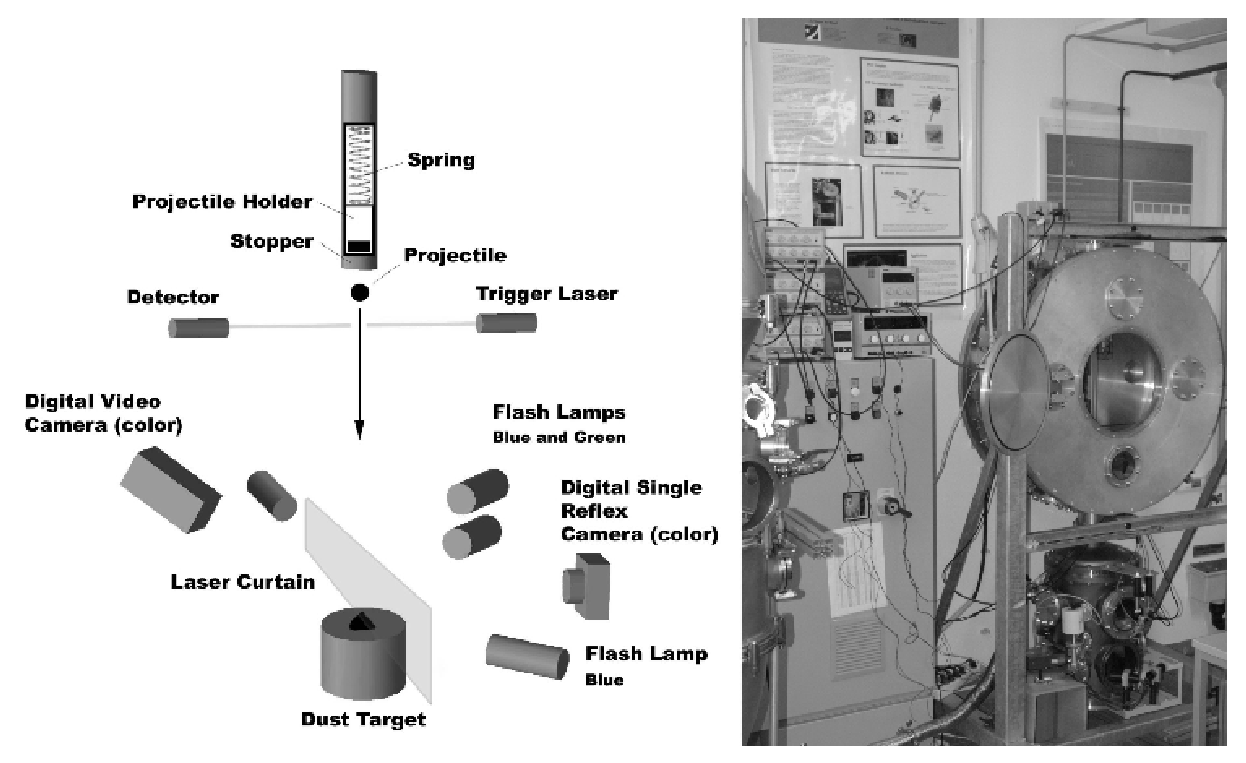
\includegraphics[width=15cm]{b2fig3.eps}}
\caption{\label{aufbau}(left) Principle of impact experiments as they have
been carried out in M\"unster.  (right) A new setup available at the
Institute of Planetology in M\"unster.  The upper right circular vacuum
chamber holds the cross bow launcher (100 m/s). The part below is the impact
chamber.}
\end{figure}


Initially different simple scenarios will be tested, e.g.\ a flat dusty
surface might be bombarded with large dust aggregates from different
arbitrary angles. We know that one dust projectile at high velocity leaves a
dust pile sticking to the target. We will study how the forming ragged
surface will react to more impacts from different angles. As addition of
individual dust particles or small aggregates at low collision velocity is
another mode of growth, we will alternatingly add layers of loose particles
and continue with large-aggregate impacts. Eventually, in an ideal case we
will carry out collisions of different kind in the sequence we expect them
under protoplanetary disk conditions. The input of the perfect sequence is
coming from the other projects within the research group, especially
\projdul{}.


Gravity is not negligible in all laboratory experiments, since the most
porous dust aggregates collapse under their own weight.  Compaction during
an impact might lead to the formation of an aggregate which is stable under
gravity.  Therefore, for collision sequences where intermediate states are
influenced by gravity, complex initial targets will be prepared artificially
to answer if e.g.\ hollow compartments below the surface are sustained after
an impact or collapse. The spatial extent of effects of a collision will be
studied. Data on individual collisions, i.e.\ size distribution of fragments
depending on the size, impact velocity, and porosity of the target body will
be distributed to the other members of the group in projects \projdul{},
\projkley{}, \projblum{}.  The fragments take part in the next
collisions. Therefore, the fragment distribution is one part of the
coagulation kernel (see \projdul{}) and determines how the size distribution
evolves over time. As all different kind of collisions happen at the same
time, it is non-trivial what collision sequence will be plausible. This
shall be closed in close collaboration with \projdul{}.

In addition, multiple impacts might be simulated in computer simulations in
project \projkley{}. This is especially important for the impact sequences
which are hardly accessible in laboratory experiments due to the strong
influence of gravity e.g for very large, very porous aggregates and high
collision velocities. Further experimental insight might be gained on
parabolic flights where ejecta are free to leave but where deceleration is
soft enough for the target to keep intact. This will allow a few ten
consecutive impacts onto one target in a single flight. Funding for such
flights will be requested elsewhere (DLR, ESA) during the course of this
project, which according to experience of past years will hopefully expand
the ground based data.

Where possible, targets will be analyzed with respect to their properties
like elasticity, sound speed, mass, morphology, porosity etc.  Some targets
will be prepared to characterize their inner morphology with respect to dust
distribution (e.g.\ pore size, local density). Analysis methods will range
from simple weighing, measuring surface morphology, analyzing morphological
changes with depth from 2-dimensional cuts to potential application of 3-D
imaging methods like X-ray or NMR Tomography in later years.

The change of permeability on a gas flow will also directly be measured in
the wind channel which is available in M\"unster.  To achieve this the
channel cross section is closed by a dust target with permeable bottom. At a
known flow rate of the wind channel and measured pressure before and after
the target the permeability can readily be obtained.  The morphology of an
evolving target will be modeled based on the results from the experiments
and calculations. This model target will be used to evaluate the flow of gas
through such a dusty body and the effect of re-accretion of dust particles.

\subsection{Schedule}
\subsubsection{First year}

In the first year first sequences of experiments with best assumptions on
dust targets and impacts will be carried out. A laser scanner will be
developed to measure the surface profile of an evolving target. To approach
a larger number of collisions simple sequences will be carried out
first. Based on their outcomes, more complex targets will be prepared to
serve as next initial target. The collisions will use the cross-bow launcher
in M\"unster and reservoirs of individual dust particles as currently
provided by a cogwheel disperser in Braunschweig. That way, collisions of
large aggregates but also phases of individual particle accumulation can be
simulated on one target. Experiments can be started as soon as the proposed
position is filled since the hardware exists and only minor adjustments are
needed.

The resulting data, e.g.\ fragment size distribution, target porosity and
cratering details will be distributed to the other groups \projblum{},
\projdul{}, and \projkley{}.  This data can be used to calculate a more
realistic size distribution (\projdul{}), to improve the simulation of
collisions and calibrate simulations which are not possible in the
laboratory (\projkley{}), and to give further input for charging experiments
(\projblum{}).  The discussion and feedback from the other groups will be a
continuous process also in the following years. Experimental results will be
fed to computer simulations while the numerical simulations in turn
determine the typical collision sequences which will be carried out in
experiments.


\subsubsection{Second year}

In accordance with the philosophy mentioned before, more realistic
collision sequences will be explored as the project proceeds. This
might not be divided in years but will evolve.

However, after the initial collision experiments permeability measurements of
typical dust targets will be carried out in the wind channel in
M\"unster. The effect of porous gas flow will be quantified and re-accretion
of particles by gas flow will be reevaluated as one source for mass gain and
surface sculpturing.

Microgravity experiments will be conducted to estimate the effect of gravity
on the impacts and the effect of elastic waves after impact into free
floating targets by observing fragments significantly away from an impact
side. This should finally lead to a formulation of an ever more realistic
description of the typical large dusty body in an evolving disk.

\subsubsection{Third year}

A database of collisions will be set up to provide the basic parameters of a
collision.  Ongoing collision experiments and gas flow experiments together
with a feedback of numerical coagulation studies (\projdul{}) should have
resulted in a more condensed view on the evolution of a larger body. The gas
flow measurements will be complemented by computer models of gas flow
through porous bodies, using commercial software (Femlab). This will be
based on recent simulations which have been carried out in M\"unster by
Paraskov et al.~(2006).  Eventually the description of a typical large body
should be defined in terms of morphology, i.e.\ density, porosity, pore
sizes, surface structure, tensile strength, elasticity, thermal properties,
etc..


\subsection{Literature}
%
% Here follows a general literature list related to the topic of the
% proposal, just like a literature list for a scientific paper.
%
% AGAIN ONLY EXAMPLES ARE LISTED NOW
%
\begin{literature}


\item Cancelliere, A., Chang, C., Foti, E., Rothman, D.H., and Succi, S. (1990) The
Permeability of a Random Medium: Comparison of Simulation with Theory,
\textit{Phys. Fluids A}, \textbf{12}, 2085

\item
Colwell, J. E. (2003)
Low velocity impacts into dust: results from the COLLIDE-2 microgravity experiment \ica, 
\textbf{164}, 188

\item
Colwell, J. E. and Taylor, M. (1999)
Low-velocity microgravity impact experiments into simulated regolith \ica, 
\textbf{138}, 241

\item Dominik, C. and Tielens,  A.~G.~G.~M. (1997) The Physics of
Dust Coagulation and the Structure of Dust Aggregates in Space
\ica, \textbf{480}, 647

\item
Hartmann, W. K. (1978)
Planet formation - Mechanisms of early growth \ica, \textbf{33}, 50

\item Koponen, A., Kataja, M., and Timonen, J. (1997) Permeability and Effective
Porosity of Porous Media \textit{PR E}, \textbf{56}, 3319

\item
Reynolds, O. (1885) On the dilatancy of media composed of rigid particles in contact 
\textit{Phil. Mag. Ser. 5}, \textbf{50}, 469 

\item Sekiya, M. and Takeda, H. (2003) Were planetesimals formed
by dust accretion in the solar nebula? \textit{Earth, Planets and
Space\/}, \textbf{55}, 263

\item Sekiya, M. and Takeda, H. (2003) Does the gas flow through
a porous dust aggregate help its growth in a protoplanetary disk?
\ica \textbf{176}, 230

\item Weidenschilling, S.~J. (1997) The Origin of Comets in the
Solar Nebula: A Unified Model \ica \textbf{127}, 290

\item Weidenschilling, S.~J. and Cuzzi, J.~N. (1993) Formation of
Planetesimals in the Solar Nebula. In: \textit{Protostars and
Planets III} (Eds. E.~H. Levy, J.~I. Lunine) University of Arizona
Press, Tucson, 1031

\item Further general literature on planetesimal (planet) formation relevant to the
project is given within the common list for the reserach group. 
 
\end{literature}



\section{External/International collaborations}
\begin{collablist}
\item[M\"unster] The IfP will be the host institute for the impact experiments.
Most experimental work and modelling of gas flows will be carried out
here. The project has access to the local facilities (see below) and technical 
support (technicians, workshop) by the department.
\item[Braunschweig] Some hardware is shared between M\"unster and
Braunschweig, e.g.\ high-speed cameras and illuminations or the
cogwheel dust disperser. A prototype of the anticipated laser
scanner was developed in Braunschweig and shall be used as the
baseline for the experiment-specific surface scanner. In addition
to that, porous dust aggregates as initial condition will be
generated in Braunschweig. 
\item[T\"ubingen] Data about the outcome
of the impacts will be compared to computer simulations done by
this group. Eventually multiple impacts not feasible in the
laboratory might be simulated complementing the experimental
results. 
\item[Heidelberg] More information about the motion and
coagulation of particles in (turbulent) disks will be provided by
these groups which will enable a better setup of collision
sequences. 
\item[Dr. J. Colwell, Boulder, USA] Dr. Colwell has
experience in collisions as well as was part in past activities of
gas aided re-accretion of dust particles. This experience will go
into determining the most realistic collision sequences and the
analysis.
\end{collablist}



\section{Link to other projects of the Forschergruppe}
\begin{linkproj}
\item[\projblum{}] As both re-accretion scenarios for dust
particles, electrostatic in project \projblum{} and aerodynamic in
project \projwurm{}, will influence the morphology of the growing
dust aggregates, a strong link between these two projects is
essential and will be established.

\item[A1,A2,B3] In line with the collaboration A1-B3, and depending on 
the influence of particle composition on the results of the coagulation
experiments, this project will also, in the later stages, 
use realistic materials such as Mg, Ca,
Al silicates and/or Fe-Ni metal for the planned coagulation experiments.

\item[\projkley{}] Results of the impacts will be compared with project
\projkley{} which performs numerical simulations of individual collisions of
porous bodies. On one side the experiments provide data as input for the
simulations. This might be used to reduce the free number of parameters in the
numerical models. On the other side the outcome of several collisions simulated
might provide initial conditions for further experiments and might expand
the region of collision sequences to parameters not accessible by laboratory
experiments.

\item[\projklahr{}] Project \projklahr{} can provide input on the typical
impact velocities expected. Since this is a free parameter in the experiments this
will also help restricting possible collision sequences better.
\item[\projdul{}] Project \projdul{} can predict which sequence of collisions
between which kind of bodies take place. The project will use the experimental results
to build a collision kernel and again to reduce the number of free parameters.
Eventually, after several feedback
loops, a more consistent picture of the typical dusty body should result.

\item[D1] The textures of agglomerates coagulated under various conditions 
can be directly compared with fine-grained, primitive chondrite assemblages
and cometary dust particles analysed with transmission electron microscopy
/SEM / TOF-SIMS/Nano-SIMS in D1.

\end{linkproj}



\section{Team members (Zusammensetzung der Arbeitsgruppe)}
%
% NOTE: Only list non-DFG-funded team members.
% NOTE: Also list technical assistants, students etc involved in the project
%
\begin{teamlist}
\item[Wurm, G., Dr. (Emmy Noether research group)]\mbox{}\\
Team leader; The project will be based on his experience in collisional physics for
planetesimal formation and the setups in his laboratory located in M\"unster.
\item[Blum, J., Prof.~Dr. (C3)]\mbox{}\\
Co-leader; Common experiment campaigns will be organized between Braunschweig and M\"unster.
\item[Krau{\ss}, O., Dr.]\mbox{}\\
Dr. Krau{\ss} is involved in the collision experiments in the laboratory in M\"unster.
He will actively take part in the experiments.
\item[Kley, W., ~Prof.~Dr. (C4)]\mbox{}\\
An intense collaboration is necessary to simulate collisions as well as to provide parameters
for experiments.
\item[Klahr, H., Dr.]\mbox{}\\
Work on possible particle/velocity distributions will provide better parameters for the
collision experiments.
\end{teamlist}
\vspace{1em}



\section{Funding requested}
The following table gives the full overview of requested
funding:\vspace{1\baselineskip}\\
%
% The table that follows is the overview over the full requested
% funding, including the positions, travel, consumables and ``other
% costs'' (which might include transportation costs of radioactive
% material or the rent of a drop tower or such).
%
\centerline{\begin{tabular}{||l|r|r|r||} \hline \hline & Year 1 & Year 2 &
Year 3 \\ \hline %
Personnel          & \hfil 24.000 &  24.000 &  24.000 \\
Consumables                        & \hfil 1.240 & \hfil 1.240 & \hfil 1.240 \\
Travel                             & \hfil 3.810 & \hfil 3.810 & \hfil 3.810 \\
Other costs                        & \hfil 1.000  & \hfil     & \hfil     \\
\hline
{\bf Total:}                       & \hfil 30.050 & \hfil 29.050 & \hfil 29.050 \\
\hline
\hline
\end{tabular}
}
\vspace{1em}\\
Below these costs are explained in more detail:

\subsection{Personnel (Personalbedarf)}
\begin{teamlist}
\item[PhD-Student (E13/2)]\mbox{}\\
While the setups for the experiments exist a dedicated project for multiple impacts requires
a person working on this full time. The experiments can best be carried out and analyzed
by a PhD student.
\end{teamlist}

\subsection{Consumables (Verbrauchsmaterial)}

For three years the following consumables are needed
\begin{itemize}
\item Oil for vacuum pumps 40 EUR/yr.
\item 300 arrows for launcher (a 5 EUR) which is 1 per experiment or
1500 EUR in total. 
(Arrows are destroyed each time due to the hard stop that ejects the dust.)
\item Material for mechanical workshop for small experimental adjustments at an estimated
500 EUR per year.
\item A few kg of dust for the experiments are estimated to 200 EUR/yr.
Since the project aims at a
self-consistent morphology we will initially use irregular dust, not special spherical particles.
\end{itemize}

\noindent
Estimated costs:\vspace{1\baselineskip}\\
 
\centerline{\begin{tabular}{||l|r|r|r||} \hline \hline & Year 1 & Year 2 &
Year 3 \\ \hline %
Oil               & \hfil     40 &     40 &  40 \\
Arrows (launcher)                  & \hfil 500 & \hfil  500 & \hfil   500 \\
Workshop                           & \hfil   500 & \hfil   500 & \hfil   500 \\
Dust                            & \hfil  200  & \hfil 200 & \hfil 200 \\
\hline
{\bf Total:}                       & \hfil  1.240 & \hfil  1.240 & \hfil 1.240 \\
\hline
\hline
\end{tabular}
}


\subsection{Travel expenses in addition to Project Z (Reisekosten)}
%
% Here only travel expenses not related to usual regular Forschergruppe
% meetings and the overall per capita budget for conferences.
%

The project requires two 2-day visits to or from T\"ubingen, Braunschweig,
and Heidelberg per year to discuss further proceedings or preparatory work.
For two persons travelling a 150 EUR (train), 70 EUR (Hotel one night) and
~30 EUR per diem (2 full or half days), this is 250 EUR per person or a total of 1500 EUR per year.

Common experiments require longer stays in Braunschweig or visits from Braunschweig.
We estimate these to be 3 weeks per year. Each week is about 300 EUR for travel
(incl. experiment hardware transport), 5 nights a 70 EUR (one person), 5 days per diem
a 24 EUR or a total of 770 EUR per week, a total of 2310 EUR per year.
%
Estimated costs
are:\vspace{1\baselineskip}\\
\centerline{\begin{tabular}{|p{18em}|p{7em}|p{7em}|}
\hline
& \hfill per year EUR& \hfill total EUR\\
\hline
Regular meetings & \hfill 1.500 & \hfill 4.500\\
\hline
Experiment campaigns & \hfill 2.310 & \hfill 6.930\\
\hline
\end{tabular}}


\subsection{Other costs (Sonstige Kosten)}

As small equipment a laser diode (line) is needed to set-up a laser scanner
for determination of the surface morphology. Estimated costs (catalogue) 1.000 EUR
in the first year.
%%%  For publication in ApJ 500 EUR are estimated in year 2 and 3.

%% Estimated costs:\vspace{1\baselineskip}\\
\centerline{\begin{tabular}{|p{15em}|p{10em}|p{7em}|}
\hline
  & \hfil  & \hfil total EUR \\
\hline
Laser&& \hfill 1.000\\
%% \hline
%% Publications&& \hfill 1.000\\
\hline
\end{tabular}}




\section{Preconditions for carrying out the project at home institution}
%
% This is one of the main subsections of a DFG Normalverfaren proposal.
% Several of the subsubsections in this subsection we have placed in their
% own subsections above (like team members, collaborations). What remains
% are the following three subsections. For those not familiar with these,
% we refer to the DFG Merkblatt on Normalverfahren-proposals.
%
\subsection{Scientific equipment available (Apparative Ausstattung)}
%
% Please list those larger instrument available to you for the project (if
% applicable also larger computer equipment in case you need substantial
% amounts of computer time).
%
\begin{compactitemize}
\item In M\"unster the experimental setups for individual collisions between mm and dm size
dust aggregates exist and can be used. This includes flash lamps, cameras, vacuum equipment, launcher,
scales, etc.

\item Computers for data analysis exist. Software (Femlab) for numerical calculations of gas flow, including gas
flow through porous dusty bodies also exists.

\item A wind channel for gas flow experiments dedicated to this kind of work can be used in
M\"unster.

\item The project has access to the analytical instruments being part of the Institute
of Planetology and Earth science department like optical microscopes and scanning
electron microscope, which can e.g.\ be used to characterize dust samples with respect
to size distribution.

\item High-speed cameras and high-speed flash-lamp illumination
will be made available to the project by the Braunschweig
laboratory.

\item The Braunschweig cogwheel dust disperser will be used for
sample preparation as well as for multiple-impact experiments in
M\"unster.

\end{compactitemize}


\subsection{Institution's general contribution (Laufende Mittel f\"ur Sachausgaben)}
%
% Please state the annual fund for consumables which comes from the
% institution's budget or any other third party  (please list separately) to
% pay for the research for which your project is part of.  Use estimates where
% applicable.
%

The project will be supported with about 500 EUR per year.



\cleardoublepage

\setcounter{equation}{0}
\setcounter{figure}{0}
%----------------------------------------------------------------------
%                        PROJECT DEFINITION
%----------------------------------------------------------------------
\renewcommand{\projnr}{B3}
\renewcommand{\projtitleshort}{High-temperature dust collision experiments}
\renewcommand{\projauth}{Blum, Trieloff}
%
\setcounter{section}{0}
\noindent{\normalfont\sffamily\Large\bfseries Project \projnr: \projtitleshort}
%
\section{Full title:}
\hspace{1\baselineskip}\\
\centerline{\large ``High-temperature dust collision
experiments''}
%\centerline{\large ''}
%
\section{General information}\mbox{}
\subsection{Principle investigators:}
\hspace{-\baselineskip}\\\noindent
%
{\bfseries\itshape Blum}, J\"urgen, Prof.~Dr.\\
C3, tenure\\
Date-of-birth: 05. April 1962, Nationality: German\\
DFG Code number of latest application: Bl 298-6/2\\
Institut f\"ur Geophysik und extraterrestrische Physik\\
Mendelssohnstr.~3\\
38106 Braunschweig\\
Tel: 0531 391 5217\\
Fax: 0531 391 8126\\
Email: j.blum@tu-bs.de\\
Private address: Wendenring 14, 38114 Braunschweig, Tel: 0531 1216432\\
%
\vspace{1em}\\\noindent
{\bfseries\itshape Trieloff}, Mario, Priv. Doz. Dr. \\
non-tenure\\
Date-of-birth: 26.2.63, Nationality: German\\
DFG Code number of latest application: TR333/8-2\\
Mineralogisches Institut der Universit�t Heidelberg\\
Im Neuenheimer Feld 236\\
69120 Heidelberg\\
Tel: 06221-546022\\
Fax: 06221-544805\\
Email: trieloff@min.uni-heidelberg.de\\
Private address:
Zaystr. 48, 76437 Rastatt
Tel: 07222/151875

\subsection{Co-investigators within this Forschergruppe:}
\begin{coilist}
\item G.~Wurm (IFP, Univ. M\"unster)
\end{coilist}


\section{Summary (Zusammenfassung)}
\subsubsection{Summary:}
Coagulation experiments shall be extended to temperatures in the
range 300-1,300~K  and to mineral phases (forsterite, enstatite,
FeNi metal, Ca,Al minerals, Fe sulfides, and Fe-bearing
olivine/pyroxene) that are expected from theoretical and
observational (both astrophysical and cosmochemical) constraints
in protoplanetary disks. In particular, the collision and adhesion
behavior at high temperatures and dust/gas ratios (sintering,
eutectic melting between immiscible phases) could be a key
mechanism to trigger agglomerate growth beyond previously
established critical sizes ($\sim$~dm) and collision velocities (a
few m/s). In addition to that, the importance of sintering for
sticking at high collision velocities shall be investigated.

\subsubsection{Zusammenfassung:}
Koagulationsexperimente sollen auf einen Temperaturbereich von 300
bis 1.300~K und auf Mineralphasen (Forsterit, Enstatit,
FeNi-Metall, Ca,Al-Minerale, Fe-Sulfide und Fe-f\"uhrende
Olivine/Pyroxene) erweitert werden, die auf Grund theoretischer
Modelle und astronomischer bzw. kosmochemischer Beobachtungen in
protoplanetaren Scheiben erwartet werden. Das Sto{\ss}- und
Adh\"asionsverhalten bei hohen Temperaturen und
Staub-Gas-Verh\"altnissen k\"onnte dabei ein
Schl\"usselmechanismus f\"ur das Agglomeratwachstum \"uber die
bislang festgestellte kritische Gr\"o{\ss}e ($\sim$~dm) und
Sto{\ss}geschwindigkeit (einige m/s) sein. Dar\"uber hinaus soll
die Bedeutung des Sinterns f\"ur die Haftung bei hohen
Sto{\ss}geschwindigkeiten untersucht werden.

\section{State of the art (Stand der Forschung)}
Coagulation experiments are crucial for our understanding of
growth from dust to planetesimals. Experiments with
micrometer-sized silica spheres (Poppe et al.~2000a) indicate that
grain-grain sticking dominates only up to relative velocities of a
few m/s. Above this threshold, grain-grain collisions do not
result in growth. Grain-grain experiments with other materials
(Poppe et al.~2000a), such as enstatite, diamond and silicon
carbide indicate similar thresholds. In the solar nebula such high
collision velocities occur mainly among larger ($\gtrsim$ dm)
agglomerates or between larger agglomerates and small dust
particles. For agglomerate-agglomerate collisions, experiments
have shown that collisions are destructive for velocities above a
few m/s (rather independently of grain material), mainly because
the weak van der Waals bonding does not provide the required
agglomerate strength/cohesion to guarantee further agglomerate
growth (Blum \& Wurm 2000; Dominik \& Tielens 1997).
Interestingly, recent experiments indicate that for collision
velocities above $\sim 10$ m/s, impacts of dust agglomerates into
compactified target agglomerates might again lead to a direct growth
(Wurm et al.~2005b). But for intermediate velocities (above a few
m/s and below $\sim 10$ m/s) no direct sticking has ever been
observed for collisions between macroscopic dust agglomerates.

A potential solution to overcome this problem might lie (1) in the
increasing strength of the van der Waals attraction with
increasing temperature ($U_{\rm vdW} \propto T$, Boyer 1975), (2)
in the process of sintering (and, thus, solidification) of dust
aggregates at elevated temperatures (Poppe 2003), or (3) in the
occurrence of eutectic melting between multi-phase agglomerates at
high (T$>300$ K) temperatures: in the region of the disk where the
terrestrial planets and asteroids were formed (within $\sim 4$
AU), disk temperatures can exceed $300$~K, and the calculation of
condensation sequences predicts the following minerals in the
inner parts of the disk: forsterite, enstatite, FeNi metal, Ca and
Al minerals, Fe sulfides, Fe-bearing olivine/pyroxene 
(Grossman \& Larimer 1974, Petaev \& Wood 1998, 2004; Lodders
2003; Gail 2003). There are some indications that agglomeration
and chondrite formation occurred under elevated dust/gas mass ratios 
(dust/gas $\sim 10$, compared to dust/gas $\sim 0.01$ as the "normal" solar value) and,
hence, under more oxidizing conditions than expected for solar
abundances (e.g.\ Sears 2004). At such enhanced dust/gas ratios, which
might occur in the midplane of the solar nebula, and elevated
temperatures prevailing in the inner disk, eutectic melting can
occur when immiscible phases (anorthite, diospide, forsterite, metal, etc.)
are in contact with each other. Melting at grain
boundaries of multi phase agglomerates, could significantly
change collision (and sticking?)  properties and internal
agglomerate strength.
%
% I added the following section(s) (Mario)
%

All above-mentioned three mechanisms cannot yet be constrained due to the
lack of experimental data with appropriate parameters. Two
experimental-parameter extensions are required: First, experiments at
elevated temperatures are needed, as all previous experiments were done at
room temperature. Second, realistic mineral mixtures are needed. Most
previous experiments were performed on glass spherules of quartz composition, 
but quartz is only expected
for fractional condensation with high isolation degree (Petaev \& Wood
\cit{1998}, \cit{2004}). In the early stage of protoplanetary disks,
expected minerals are forsterite, enstatite, FeNi metal, Ca and Al minerals (Melilite, anorthite, diopside)
Fe sulfides, Fe-bearing olivine/pyroxene (Grossman \& Larimer 1974, Petaev
\& Wood 1998, 2004; Lodders 2003; Gail 2003). Material/Mineral properties
may strongly influence sticking mechanisms listed under 1-3 above,
particular mechanism 3 (eutectic melting) only works in a multi-phase
system. Thus, the lack of multi-mineral experiments is a serious limitation
for present models of planetesimal formation.

Scenarios integrating short-lived nuclide chronometries (Kleine et
al.~\cit{2005}; Bizzarro et al.~\cit{2004}) and short-lived nuclide heating
of planetesimals (Trieloff et al.~\cit{2003}) indicate that meteorite parent
bodies formed over the first 4 Myr in the solar nebula (Sears 2004; Trieloff and Palme
2006). This is not as fast as theoretically possible and highlights the
importance that planetesimal growth may be delayed (and then overcome) at
certain specific conditions in the solar nebula (and by analogy in
protoplanetary disks), possibly by conditions and/or mechanisms to be
investigated here.


\section{Preliminary work (Eigene Vorarbeiten)}

%\begin{figure}
%\centerline{\includegraphics[width=8cm]{myfig.eps}}
%\caption{}
%\end{figure}

Scientists in the Institute for Geophysics and extraterrestrial
Physics have extended experience in dust-collision and
dust-aggregation experiments. Earlier work on dust-dust
interactions comprises measurements on cohesion and friction
forces between micrometer-sized dust particles (Heim et al.~1999,
2005), on the sticking probabilities of micrometer-sized dust
grains of various shapes and compositions (Poppe et al.~2000a), on
the formation of fractal dust agglomerates due to Brownian motion
(Blum et al.~2000; Krause \& Blum 2004), sedimentation (Blum et
al.~1999), and gas turbulence (Wurm \& Blum 1998), on impact
compaction and fragmentation of fractal dust aggregates (Blum \&
Wurm 2000), and on impacts of dust agglomerates into dusty targets
(Langkowski \& Blum, in preparation).

For this proposal, the pioneering experiments on the collision and
sticking behavior of single, micrometer-sized dust grains by Poppe
et al.~(2000a) shall be extended to above room temperatures. In the
experiments by Poppe et al.~(2000a), a powder sample of
well-characterized dust particles was deagglomerated by a
fast-rotating cogwheel (Poppe et al.~1997) and accelerated to
velocities $\lesssim 50$~m/s. Individual dust-particle collisions
with flat target surfaces (at arbitrary impact angle) could be
observed by high-speed imaging through a long-distance microscope
and stroboscopic laser illumination. This technique allows the
determination of the collision velocity as well as (in the case of
non-sticking collisions) the measurement of the rebound velocity,
rebound angle, and charge transfer (Poppe et al.~2000b; Poppe \&
Schr\"apler 2005) between projectile and target (see project
\projblum{}). It turned out that spherical projectiles have a
well-defined threshold velocity for sticking which increases with
decreasing particle size. Typical threshold velocities are a few
m/s for spherical, micrometer-sized $\rm SiO_2$ grains. Irregular
particles of micrometer size show a much smoother transition from
high sticking efficiencies at low velocities to low sticking
probabilities at high impact speeds. This effect is caused by the
random orientation of the particle at the moment of contact. Tips
and edges preferentially lead to particle rebound, while flat
surfaces in contact enhance the chance for sticking. It should be
emphasized that all above experiments were carried out at room
temperatures and with refractory dust grains. As we expect a
temperature influence on the strength of the van der Waals
attraction between the grains in contacts as well as on the
``hardness'' (elasticity and plasticity) of the grains, the work
described in this proposal is essential for a thorough
understanding of the growth processes in protoplanetary disks.

In another set of experiments, Poppe (2003) investigated the
influence of elevated temperatures on the structure of
high-porosity dust aggregates consisting of spherical $\rm SiO_2$
particles. The samples were heated in an oven at varying
temperatures and heating durations and were then analyzed by
scanning electron microscopy. Surface diffusion, sintering, and
viscous flow were identified as important transformation
mechanisms in grain-grain contacts. Surface diffusion dominates at
the start of restructuring and viscous flow at higher
temperatures. The formation and growth of inter-particle necks was
observed and could be described by a sintering model. Between the
temperature of neck formation and that of melting, further
restructuring occurs which leads to the dissolution of the
particulate structures and to a compactification of the aggregates.

A method for the formation of macroscopic (cm-sized), monolithic,
and high-porosity dust aggregates that resemble the predicted
morphologies and properties of pre-planetesimal dust aggregates
was established by Blum \& Schr\"apler (2004) who used random
ballistic deposition (RBD)  of individual dust grains. A variety
of studies with these RBD agglomerates for the determination of
their mechanical (Blum \& Schr\"apler 2004; Heim et al.~2005) and
their collision properties (see below) have been carried out.
Studies of the thermal and optical properties of these RBD
agglomerates are under way.

Impacts of mm-sized projectiles into cm-sized, high-porosity dust
aggregates were studied by Langowski \& Blum (in preparation) for
dusty projectiles and by Teiser \& Blum (in preparation) for solid
projectiles. Due to the overwhelming influence of gravity on the
outcome of the collision, these experiments were exclusively
carried out under microgravity conditions. It turned out that
both, solid and aggregated projectiles, stick to the target
agglomerate for not too oblique impacts in the velocity range $0
\ldots \sim 3$~m/s, while rebound and mass transfer was observed
for oblique impacts. An experimental extension for impact
velocities up to $\sim 20$~m/s is foreseen for the near future.
%
% I added the following section(s) (Mario)
%

Co-PI Mario Trieloff is working in the research area of cosmochemistry and
geochemistry, particular the isotope chronology of processes in the
early solar system and their relationship to astrophysical processes in
protoplanetary disks. M. Trieloff conducted a number of studies on early
meteorite chronology and the accretionary history of planetesimals,
i.e.\ meteorite parent bodies (Trieloff et al.~\cit{2003}; Kunz et al.~1995;
Pellas et al.~1997; Korochantseva et al.~2005). He also studied processes
that relate to disk clearing and solar wind implantation into precursor
planetesimals of meteorite parent bodies and the terrestrial planets
(Trieloff et al.~\cit{2000}, \cit{2002}; Trieloff and Kunz 2005; Schwarz et
al.~2005).  Trieloff and Palme 2006 reviewed and outlined the early solar
system history.

M. Trieloff has particular experience with high-temperature
furnaces and ultra-high-vacuum technology for noble gas extraction
from solids, and mass spectrometric analysis for which in-house
constructed high-temperature furnaces are used. Experience with
and control of heated and evacuated devices will be of particular
benefit for the studies proposed here.

%
% Here follows the own refereed publications by the PIs in relation to
% the project proposed here.
%
\ownpubltitle{Own publications related to the Forschergruppe:}
%
% BELOW IS ONLY AN EXAMPLE OF TWO ENTRIES. SEE THE ADDITIONAL FILES
% SENT TO YOU WITH ALL THE REFERENCES FROM THE VORANTRAG
%
\begin{ownpubl}

\item Blum, J., Wurm, G., Poppe, T. and Heim, L.-O. (1999) Aspects
of Laboratory Dust Aggregation with Relevance to the Formation of
Planetesimals. In: \textit{Laboratory Astrophysics and Space
Research}, Astrophysics and Space Science Library, Vol. 236 (Eds.
P. Ehrenfreund, K. Krafft, H. Kochan, V. Pirronello) Kluwer
Academic Publishers, Dordrecht, 399

\item Blum, J. and Wurm, G. (2000) Experiments on Sticking,
Restructuring and Fragmentation of Preplanetary Dust Aggregates.
\ica, \textbf{143}, 138

\item Blum, J., Wurm, G., Kempf, S., Poppe, T., Klahr, H., et al.
(2000) Growth and Form of Planetary Seedlings: Results from a
Microgravity Aggregation Experiment. \prl, \textbf{85}, 2426

\item Blum, J. and Schr\"apler, R. (2004) Structure and Mechanical
Properties of High-Porosity Macroscopic Agglomerates Formed by
Random Ballistic Deposition, \prl, \textbf{93}, 115503

\item Heim, L.-O., Blum, J., Preuss, M. and Butt, H.-J. (1999)
Adhesion and Friction Forces Between Spherical Micrometer-Sized
Particles. \prl, \textbf{83}, 3328

\item Heim, L.-O., Butt, H.-J., Schr\"apler, R. and Blum, J. (2005)
Analyzing the Compaction of High-Porosity Microscopic
Agglomerates, \textit{Australian Journal of Chemistry\/},
\textbf{58(9)} 671

\item Korochantseva, E.~V., Trieloff M., Buikin A.~I., Meyer H.~P.
and Hopp J. (2005) Argon-40/Argon-39 dating, and cosmic ray
exposure time of desert meteorites: Dhofar 300 and Dhofar 007
eucrites and anomalous achondrite NWA 011, \textit{Meteoritics and
Planetary Science \/} \textbf{40}, 1433

\item Krause, M. and Blum J., (2004) Growth and Form of Planetary
Seedlings: Results from a Sounding Rocket Microgravity Aggregation
Experiment. \prl, \textbf{93}, 021103

\item Kunz J., Trieloff M., Bobe K., Metzler K., St\"offler D. and
Jessberger E.~K. (1995) The collisional history of the HED parent
body inferred from 40Ar-39Ar ages of Eucrites. \textit{Planetary
and Space Science\/} \textbf{43}, 527

\item Pellas P., Fieni C., Trieloff M. and Jessberger E.~K. (1997)
The cooling history of the Acapulco meteorite as recorded by the
244Pu and 40Ar-39Ar chronometers. \textit{Geochimica et
Cosmochimica Acta\/} \textbf{61}, 3477

\item Poppe, T., Blum, J. and Henning, Th. (1997) Generating a jet
of deagglomerated small particles in vacuum. \textit{Review of
Scientific Instruments\/}, \textbf{68}, 2529

\item Poppe, T., Blum, J. and Henning, Th. (2000a) Analogous
Experiments on the Stickiness of Micron-Sized Preplanetary Dust.
\apj, \textbf{533}, 454

\item Poppe, T., Blum, J. and Henning, Th. (2000b) Experiments on
Collisional Grain Charging of Micron-sized Preplanetary Dust.
\apj, \textbf{533}, 472

\item Poppe, T. (2003) Sintering of highly porous silica-particle
samples: analogues of early Solar-System aggregates. \ica,
\textbf{164}, 139

\item Poppe, T. and Schr\"apler, R. (2005) Further Experiments on
Collisional Tribocharging of Cosmic Grains. \aap, \textbf{438}, 1

\item Schwarz W.~H., Trieloff M. and Altherr R. (2005) Subduction
of solar type noble gases from extraterrestrial dust: Constraints
from high-pressure low-temperature metamorphic deep sea sediments,
\textit{Contributions to Mineralogy and Petrology\/} \textbf{149},
675

\item Trieloff M. and Kunz J. (2005) Isotope systematics of noble
gases in the Earth�s mantle: Possible sources of primordial
isotopes and implications for mantle structure. \textit{Physics of
the Earth and Planetary Interiors\/} \textbf{148}, 13

\item Trieloff M. and Palme H. (2006) The origin of solids in the
early solar system. In: \textit{Planet Formation -� Theory,
Observations, and Experiments} (Eds. H. Klahr, W. Brandner)
Cambridge University Press, Cambridge, 64

\item Trieloff M., Jessberger E.~K., Herrwerth I., Hopp J.,
Fi\'{e}ni C., Gh\'{e}lis M., Bourot-Denise M. and Pellas P. (2003)
244Pu and 40Ar-39Ar thermochronometries reveal structure and
thermal history of the H-chondrite parent asteroid.
\textit{Nature\/} \textbf{422}, 502

\item Trieloff M., Kunz J. and All\`{e}gre C.~J. (2002) Noble gas
systematics of the R\'{e}union mantle plume source and the origin
of primordial noble gases in Earth�s mantle. \textit{Earth and
Planetary Science Letters\/} \textbf{200}, 297

\item Trieloff M., Kunz J., Clague D.A., Harrison D. and
All\`{e}gre C.J. (2000) The nature of pristine noble gases in
mantle plumes. \textit{Science\/} \textbf{288}, 1036

\item Wurm, G. and Blum, J. (1998) Experiments on Preplanetary
Dust Aggregation. \ica, \textbf{132}, 125
%
% I added the following references (Mario)
%



\end{ownpubl}
%
\section{Goals (Ziele)}

It is the utmost goal of the proposed study to investigate the
influence of elevated temperatures on the collision and sticking
behavior of dust particles and dust agglomerates. We expect
considerable changes of these properties due to an increased van
der Waals force at higher temperatures, due to the occurrence of
sintering within dust aggregates, and due to the possibility of
eutectic melting in collisions between dust grains of different
mineralogical composition. The results of our experimental
investigations shall be included in models of the evolution of the
solid bodies in protoplanetary disks. The following individual
goals have been identified and will be addressed by project
\projblumtrie{}:

\begin{itemize}

\item Study the collision behavior and sticking probabilities in
single-grain impacts in the temperature range from 300~K to
1,300~K and in the velocity range $0 \ldots 50$~m/s. Grain sizes
should range from sub-micrometer to centimeter and grain materials
should comprise of forsterite, enstatite, FeNi metal, Ca,Al
minerals, Fe sulfides, and Fe-bearing olivine/pyroxene. Grain and
target materials should be identical to understand simple mono-phase systems first.

\item Investigate the influence of sintering on the morphology and
mechanical properties (compressive strength, tensile strength) of
high-porosity dust aggregates. Aggregates will be produced by the
RBD process and will consist of micrometer-sized grains.
Individual dust grains will be of mono-phase type, consisting of
forsterite, enstatite, FeNi metal, Ca,Al minerals, Fe sulfides,
and Fe-bearing olivine/pyroxene. 
%These experiments shall study the
%evolution of early dust aggregates in protoplanetary disks before
%extensive mixing or cooling occurs.

\item Study the influence of elevated temperatures on the
structure of aggregates consisting of two-phase minerals and the
occurrence of eutectic melting inside mixed-phase aggregates. This
is relevant for those stages of the protoplanetary disk when
multiple grain materials coexist due to radial mixing or cooling.

\item Understand the collision behavior of realistic multi-phase
mixtures at various temperatures from below to above eutectic
melting points. When two aggregates consisting of different
mineral phases (e.g.\ anorthite, diopside, forsterite) collide at temperatures above the
eutectic melting point (but below the melting point of the
mono-phase minerals), contact melting can occur and can increase
the threshold velocity for sticking. The efficiency of this effect
shall be investigated.

\item Quantify the outcome of collisions for the parameter space
comprising of grain material, grain temperature, impact velocity,
and impact angle in order to use it for astrophysical coagulation
modelling at various evolutionary $(p, T, t)$ stages of
protoplanetary disks (see project \projdul{}).

\end{itemize}


\section{Work schedule (Arbeitsprogramm)}
\subsection{Methods}

We will concentrate on the three most abundant grain materials
that are predicted by condensation-sequence calculations (Petaev
\& Wood \cit{1998}; Sears 2004; 
Grossman \& Larimer {1974}):
%
% I added the references in last line above (Mario)
%
\begin{itemize}
    \item Mg silicates,
    \item Metals (Fe/Ni) and their sulfides,
    \item Ca/Al silicates.
\end{itemize}
Mineral and grain-size separates will be prepared at the
Mineralogical Institute of the University of Heidelberg by
milling, sieving and centrifugation techniques that are already
available. The resulting dust-particle fractions will be analyzed
by SEM with respect to grain-size distribution and grain/surface
morphology.
%
% I added the following section (Mario)
%

As starting materials we will use either synthesized, commercially
available (e.g.\ Crystec GmbH, Berlin/ SPI supplies) or natural materials
(SPI Supplies/C.M. Taylor collection), which are also used for project \projlattard{}. They will be checked for homogeneity
and purity by EMP and possibly by ion microprobe, all
equipment available at the Mineralogical Institute Heidelberg. We expect to succeed in 
obtaining appropriate material, however, in the case these materials have
not the desired level of homogeneity and purity, the synthesis of crystals
can also be performed by high temperature experiments under controlled
oxygen fugacity, either via solid state reactions or in the presence of a
melt phase or a flux. Respective high temperature furnaces are available at
the Mineralogical Institute, or via cooperations with labs specialized in
mineral synthesis.

In a first step, we will produce high-porosity dust aggregates by
the RBD method. Dust aggregates will consist of single minerals
and of mixtures with an emphasized eutectic melting
behavior. Of particular interest is the system Anorthite-Diopside-Forsterite (Hughes 1982; Osborn and Tait 1952; Bowen 1915). Ca,Al minerals are the first condensates to be expected in a high temperature solar nebula. Anorthite and Diopside (to be exact, the Ti-rich variety fassaite) are � besides melilite and spinel - major constituents of Ca,Al rich inclusions (CAIs), the oldest objects from the early solar system. Anorthite and diopside are stable at decreasing temperatures when the Mg-silicates forsterite and enstatite start to condense (Grossman \& Larimer 1974, Petaev\& Wood 1998, 2004; Lodders 2003; Gail 2003), which represent the major mass fraction of silicate material in the solar nebula.

To study the influence of sintering and eutectic melting on the structure of
the dust aggregates for a large variety of dust materials (in the
work by Poppe (2003), only $\rm SiO_2$ was used), the samples will
be heated in a vacuum furnace at a given temperature and for a
pre-set heating duration. Hereafter, they will be recovered for
analytical inspection by optical and secondary electron microscopy
(and also by thin sectioning and electron microprobe analysis
to determine changes in chemical composition at grain boundaries).
Macroscopic samples will also be analyzed with respect to changes
in their mechanical properties (compressive and tensile
strengths); microscopic samples can be studied under the electron
microscope using the nano-manipulator of the Max Planck Institute
for Polymer Research in Mainz.

While these experiments are under way, the existing experimental
setup for the investigation of the collision and sticking behavior
of single, micrometer-sized dust particles will be adapted to
allow high-temperature studies. The sample reservoir, the cogwheel
deagglomerator and accelerator, and the target holder will be
equipped with inductive heaters and temperature sensors. For
thermal insulation of the experiment, the components will be
transferred to a high-vacuum tank (possibly with water cooling).
High-vacuum conditions are required for thermal insulation of the
experimental setup from the hot interior. In addition to that,
oxidization of the minerals will be efficiently prevented. After
completion of the setup, systematic impact experiments of dust
particles consisting of the above-mentioned materials with targets
of identical or different materials will be conducted. Experiments
will start at room temperature and will then be extended to
1,300~K. Changes in the collision and sticking behavior, e.g.\
decreased rebound velocity or increased threshold velocity for
sticking, will be observed through microscopic monitoring of
individual impacts. A difficulty arises from the extremely short
radiation cooling timescales of free micrometer-sized particles of
only a few milliseconds for very hot dust grains. Possible
countermeasures are very short experiment durations (possible for
high-velocity impacts $\gtrsim 10$~m/s or a radiation equilibrium
between particles and environment, which can be reached by a hot
enshrouding of the interaction volume.

For mineral pairs for which eutectic melting in collisions is
expected, we will also setup an accelerator for projectiles in the
size range from 0.1 to 10~mm. Impacts of these macroscopic
particles will be observed by high-speed imaging using telecentric
optics. For these particle sizes, the cooling timescales of free
particles are much longer than an individual experiment duration.
After the collision experiments, the particles will be sampled and
their surfaces will be analyzed by SEM. A model for the
physico-chemical behavior of the contacting dust particles will be
developed and compared to the results of the collision
experiments.

In the following project stages, we will investigate collisions
among macroscopic dust aggregates (including sintered aggregates)
at elevated temperatures. In principle, we have three types of
aggregate-aggregate experiments available for the study of (1) the
collision behavior between mm-sized agglomerates in the velocity
regime between $\sim 0.5$ m/s and $\sim 20$ m/s (Braunschweig),
(2) impacts of mm-sized agglomerates into high-porosity cm-sized
agglomerates for velocities in the range $\sim$ 0.5 m/s \dots\ $\sim$ 20 m/s
(Braunschweig), and (3) impacts of cm-sized agglomerates into
dm-sized target agglomerates of intermediate to low porosities in
the velocity range from $\sim 10$ m/s to $\sim 100$ m/s
(M\"unster). For the impact and collision experiments at higher
temperatures, heating facilities for projectiles and targets must
be developed and implemented. Depending on the experimental
results, it could become necessary to perform the impact and
collision experiments under microgravity conditions. Therefore, we
will foresee two drop-tower campaigns. The existing
(room-temperature) experiments in Braunschweig and M\"unster are
already microgravity-compatible.

In the final stage, we will incorporate the experimental results
on the influence of elevated temperatures, sintering, and eutectic
melting into dust coagulation models for protoplanetary disks (see
project \projdul{}). This will be done in close cooperation with
the other groups involved in this Forschergruppe.

The groups in Braunschweig and M\"unster have worldwide unique experimental
equipment and expertise in coagulation experiments and preparation of high-
and low-porosity dust samples (see e.g.\ Wurm \& Blum 1998, Blum et
al.~1999, Blum et al.~2000, Blum \& Wurm 2000, Wurm \& Blum 2000, Wurm et
al.~2001, Krause \& Blum 2004, Blum \& Schr\"apler 2004, Wurm et al.~2005a,
2005b). This expertise will be interdisciplinarily combined with the
mineralogical and cosmochemical expertise of the group at the Mineralogical
Institute in Heidelberg, which has general broad experience in analytical
and experimental mineralogy and petrology, and also particular expertise in
studying meteorites, and their inferences on the chronology and conditions
of planetesimal accretion in the early solar system (e.g.\ Trieloff et al.~2003).


\subsection{Schedule}
\subsubsection{First year}
%
% I added the following section (Mario)
%
Mineral and grain-size separates will be prepared at the
Mineralogical Institute of the University of Heidelberg by
appropriate techniques (mineral separation, milling, sieving, etc.). As
materials we will use either synthesized, commercially
available (e.g.\ Crystec GmbH, Berlin/ SPI supplies) or natural materials
(SPI Supplies/C.M. Taylor collection), see also project \projlattard{}. If necessary, appropriate minerals can also be synthesized by
high-temperature devices under controlled oxygen fugacity.
Chemical homogeneity and purity will be controlled by secondary
electron microscopy and electron microprobe (if additionally
needed, the ion microprobe) techniques, all equipment available at
the Mineralogical Institute Heidelberg.

With the samples from Heidelberg, room-temperature RBD experiments
for the formation of macroscopic dust aggregates will be
performed. These samples will be heated in vacuum furnaces in
Heidelberg and studied with respect to
morphological/mineralogical/chemical (Heidelberg) and mechanical
(Braunschweig, Mainz) changes. Parallel to these experiments, the
experimental setup for the study of individual collisions of
micrometer-sized grains with flat targets will be adapted to
higher temperatures.

\subsubsection{Second year}
Systematic experiments on the impact and coagulation behavior of
single, micro\-me\-ter-sized dust grains will be conducted for
velocities $\lesssim 50$~m/s and temperatures $300 \ldots 1,300$~K
with mono-phase and binary-phase materials. In addition to that,
we will start to adapt the impact and collision experiments of
dust aggregates to higher temperatures.

\subsubsection{Third year}
Systematic experiments on the collision behavior of mono-phase and
binary-phase dust aggregates will be conducted at elevated
temperatures. The result of the experiments will enable us to
determine the importance and impact of eutectic melting for the
sticking properties of protoplanetary dust aggregates. Finally,
the transfer of the experimental results to protoplanetary
coagulation models will be realized in close cooperation with the
other groups of this Forschergruppe. Publication of the results
closes this work.

\subsection{Literature}
%
% Here follows a general literature list related to the topic of the
% proposal, just like a literature list for a scientific paper.
%
% AGAIN ONLY EXAMPLES ARE LISTED NOW
%
\begin{literature}

\item Bizzarro, M., Baker, J. A. and Haack, H. (2004).  Mg isotope evidence
for contemporaneous formation of chondrules and refractory inclusions,
\textit{Nature} \textbf{431}, 275--278.

\item Blum, J., Wurm, G., Poppe, T. and Heim, L.-O. (1999) Aspects
of Laboratory Dust Aggregation with Relevance to the Formation of
Planetesimals. In: \textit{Laboratory Astrophysics and Space
Research}, Astrophysics and Space Science Library, Vol. 236 (Eds.
P. Ehrenfreund, K. Krafft, H. Kochan, V. Pirronello) Kluwer
Academic Publishers, Dordrecht, 399

\item Blum, J. and Wurm, G. (2000) Experiments on Sticking,
Restructuring and Fragmentation of Preplanetary Dust Aggregates.
\ica, \textbf{143}, 138

\item Blum, J., Wurm, G., Kempf, S., Poppe, T., Klahr, H., et al.
(2000) Growth and Form of Planetary Seedlings: Results from a
Microgravity Aggregation Experiment. \prl, \textbf{85}, 2426

\item Blum, J. and Schr\"apler, R. (2004) Structure and Mechanical
Properties of High-Porosity Macroscopic Agglomerates Formed by
Random Ballistic Deposition, \prl, \textbf{93}, 115503

\item Bowen, N.L. (1915) The crystallization of haplobasaltic, haplodioritic, and related magmas. Am. J. Sci. 4th Ser. \textbf{40}, 161

\item Boyer, T.H. (1975) Temperature Dependence of Van der Waals
Forces in Classical Electrodynamics with Classical Electromagnetic
Zero-Point Radiation, Phys. Rev. A, \textbf{11}, 1650

\item Dominik, C. and Tielens,  A.~G.~G.~M. (1997) The Physics of
Dust Coagulation and the Structure of Dust Aggregates in Space.
\ica, \textbf{480}, 647

\item Gail, H.-P. (2003) Formation and Evolution of Minerals in
Accretion Disks and Stellar Outflows. In:
\textit{Astromineralogy}, Lecture Notes in Physics Vol. 609 (Ed.
Th. Henning), Springer, Heidelberg. 55

\item Grossman, L. \& Larimer, J.~W. 1974 Early chemical history of the
Solar System. Rev. Geophys Space Phys. \textbf{12}, 71-101

\item Heim, L.-O., Blum, J., Preuss, M. and Butt, H.-J. (1999)
Adhesion and Friction Forces Between Spherical Micrometer-Sized
Particles. \prl, \textbf{83}, 3328

\item Heim, L.-O., Butt, H.-J., Schr�pler, R. and Blum, J. (2005)
Analyzing the Compaction of High-Porosity Microscopic
Agglomerates, Australian Journal of Chemistry, \textbf{58(9)} 671

\item Hughes C.J. (1982) Igneous Petrology. Elsevier, Amsterdam, 551pp. 

\item Kleine, T., Mezger, K., Palme, H., Scherer, E. and M\"unker,
C.\ (2005).  Early core formation in asteroids and late accretion of
chondrite parent bodies: Evidence from 182Hf-182W in CAIs, metal-rich
chondrites and iron meteorites.  \textit{Geochim. Cosmochim. Acta}, \textbf{69} 5805. 

\item Korochantseva, E.~V., Trieloff M., Buikin A.~I., Meyer H.~P.
and Hopp J. (2005) Argon-40/Argon-39 dating, and cosmic ray
exposure time of desert meteorites: Dhofar 300 and Dhofar 007
eucrites and anomalous achondrite NWA 011, \textit{Meteoritics and
Planetary Science \/} \textbf{40}, 1433

\item Krause, M. and Blum J., (2004) Growth and Form of Planetary
Seedlings: Results from a Sounding Rocket Microgravity Aggregation
Experiment. \prl, \textbf{93}, 021103

\item Kunz J., Trieloff M., Bobe K., Metzler K., St\"offler D. and
Jessberger E.~K. (1995) The collisional history of the HED parent
body inferred from 40Ar-39Ar ages of Eucrites. \textit{Planetary
and Space Science\/} \textbf{43}, 527

\item Lodders, K. (2003) Solar System Abundances and Condensation
Temperatures of the Elements. \apj, \textbf{591}, 1220

\item Osborn, E.F. and Tait D.B. (1952) The system diopside-forsterite-anorhtite. \textit{Am. J. Sci., Bowen Vol.}
\textbf{250A}, 413.

\item Petaev, M. I. and J. A. Wood (1998) The Condensation with Partial
Isolation (CWPI) model of nebular condensation in the Solar Nebula.
\textit{Meteorit. Planet. Sci.}
\textbf{33}, 1123-1137.

\item Petaev, M. I. and  Wood, J. A. (2004) Meteoritic constraints on
temperatures, pressures, cooling rates, chemical compositions, and modes of
condensation in the solar nebula. In Chondrites and the Protoplanetary Disk
(Eds. A.~N.  Krot, E.~R.~D. Scott, and B. Reipurth), Vol. 341.

\item Pellas P., Fieni C., Trieloff M. and Jessberger E.~K. (1997)
The cooling history of the Acapulco meteorite as recorded by the
244Pu and 40Ar-39Ar chronometers. \textit{Geochimica et
Cosmochimica Acta\/} \textbf{61}, 3477

\item Poppe, T., Blum, J. and Henning, Th. (1997) Generating a jet
of deagglomerated small particles in vacuum. \textit{Review of
Scientific Instruments\/}, \textbf{68}, 2529

\item Poppe, T., Blum, J. and Henning, Th. (2000a) Analogous
Experiments on the Stickiness of Micron-Sized Preplanetary Dust.
\apj, \textbf{533}, 454

\item Poppe, T., Blum, J. and Henning, Th. (2000b) Experiments on
Collisional Grain Charging of Micron-sized Preplanetary Dust.
\apj, \textbf{533}, 472

\item Poppe, T. (2003) Sintering of highly porous silica-particle
samples: analogues of early Solar-System aggregates. \ica,
\textbf{164}, 139

\item Poppe, T. and Schr\"apler, R. (2005) Further Experiments on
Collisional Tribocharging of Cosmic Grains. \aap, \textbf{438}, 1

\item Schwarz W.~H., Trieloff M. and Altherr R. (2005) Subduction
of solar type noble gases from extraterrestrial dust: Constraints
from high-pressure low-temperature metamorphic deep sea sediments,
\textit{Contributions to Mineralogy and Petrology\/} \textbf{149},
675

\item Sears, D. (2004) The origin of chondrules and chondrites.
Cambridge: Cambridge University Press

\item Trieloff, M., Jessberger, E.~K., Herrwerth, I., Hopp, J.,
Fi\'eni, C., Gh\'elis, M., Bourot-Denise, M. and Pellas, P. (2003)
$^{244}$Pu and $^{40}$Ar-$^{39}$Ar thermochronometries reveal
structure and thermal history of the H-chondrite parent asteroid.
\nat, \textbf{422}, 502

\item Trieloff M. and Kunz J. (2005) Isotope systematics of noble
gases in the Earth�s mantle: Possible sources of primordial
isotopes and implications for mantle structure. \textit{Physics of
the Earth and Planetary Interiors\/} \textbf{148}, 13

\item Trieloff M. and Palme H. (2006) The origin of solids in the
early solar system. In: \textit{Planet Formation -� Theory,
Observations, and Experiments} (Eds. H. Klahr, W. Brandner)
Cambridge University Press, Cambridge, 64

\item Wurm, G. and Blum, J. (1998) Experiments on Preplanetary
Dust Aggregation. \ica, \textbf{132}, 125

\item Wurm, G. and Blum, J. (2000) An Experimental Study on the
Structure of Cosmic Dust Aggregates and Their Alignment by Motion
Relative to Gas. \apj, \textbf{529}, L57

\item Wurm, G., Blum, J. and Colwell, J.~E. (2001) Aerodynamical
sticking of dust aggregates. \phre, \textbf{64}, 046301

\item Wurm, G., Paraskov, G. and Krauss, O. (2005a) Ejection of
dust by elastic waves in collisions between millimeter- and
centimeter-sized dust aggregates at 16.5 to 37.5 m/s impact
velocities. \phre, \textbf{71}, 21304

\item Wurm, G., Paraskov, G. and Krauss, O. (2005b) Growth of
Planetesimals by Impacts at ~25m/s. \ica, \textbf{178}, 253




\end{literature}



\section{External/International collaborations}
\begin{collablist}


\item[MPIP Mainz] Dr. L.-O. Heim and Prof. H.-J. Butt (Max Planck
Institute for Polymer Research, Mainz) will aid with their
expertise on the micro-manipulation of small particles and their
knowledge about interaction (adhesion, friction) forces between
such particles.

\item[TU Braunschweig] Dr. M. Morgeneyer (Institute for Particle
Technology) will help to analyze the sintered dust samples with
respect to their mechanical properties.

\end{collablist}



\section{Link to other projects of the Forschergruppe}
\begin{linkproj}


\item[\projtscharn{},\projlattard{}] Projects \projtscharn{} and
\projlattard{} will provide input on abundances of various
minerals to be expected at various parts of the disk. Due to the
detailed chemical and mineralogical modelling in projects
\projtscharn{} and \projlattard{}, much better constraints on the
abundances of the minerals will be available to project
\projblumtrie{}. Thus, the laboratory experiments in project
\projblumtrie{} can always be carried out with dust particles
produced under state-of-the-art knowledge on their relevance.

\item[\projblum{},\projwurm{}] A strong collaborate effort between
the three experimental projects \projblum{},\projwurm{}, and
\projblumtrie{} is mandatory for a successful mapping of the
parameter space for protoplanetary dust agglomeration. Due to
personal and institutional overlap of these three projects, a
strong interaction will be guaranteed.

\item[\projkley{}] Information about the temperature dependence of
the collision behavior of protoplanetary dust aggregates will be
useful and valuable information for the development of the SPH
aggregate collision code to be developed in \projkley{}.

\item[\projklahr{}] Project \projklahr{} will provide input on the
typical impact velocities expected for macroscopic
protoplanetesimal bodies and, thus, for the planning of the
experiments in project \projblumtrie{}.

\item[\projdul{}] The experiments in project \projblumtrie{} will
provide valuable input parameters for the dust-dust interactions
for project \projdul{} and will help to define the reaction and
coagulation kernel in Smoluchowski's equation which is the basis
for project \projdul{}. Vice versa, project \projdul{} will be
able to predict aggregate abundances, collision probabilities and
collision velocities in protoplanetary disks, which all are
important input parameters for the experiments in project
\projblumtrie{}. As part of the project, an extensive iteration
between laboratory work and modelling efforts is envisioned.

\item[D1] The textures of agglomerates coagulated under various conditions 
can be directly compared with fine-grained, primitive chondrite assemblages
and cometary dust particles analysed with transmission electron microscopy
/SEM / TOF-SIMS/Nano-SIMS in D1.

\end{linkproj}



\section{\label{persb3}Team members (Zusammensetzung der Arbeitsgruppe)}
%
% NOTE: Only list non-DFG-funded team members.
% NOTE: Also list technical assistants, students etc involved in the project
%
\begin{teamlist}

\item[Blum, J., Prof.~Dr. (C3)]\mbox{}\\
Team leader. Overlooks the experimental and modelling efforts and
supervises the PhD student funded through this project. Provides
extensive expertise in dust collisions, high-speed imaging
techniques, and microgravity experimentation.

\item[Trieloff, M., Priv. Doz. Dr.]\mbox{}\\
Team leader of isotope geochronology group. Supervises mineral
preparation, agglomerate heating studies and analytical studies
using SEM, EMPA, and SIMS.

\item[Wurm, G., Dr.]\mbox{}\\
Team collaborator. Hosts the PhD student for high-temperature
impact experiments of large dust aggregates. Provides expertise in
high-velocity dust impacts and microgravity experimentation.

\item[Altherr, R., Prof. Dr. (C4)]\mbox{}\\
Internal collaborator. Will assist in petrological/mineralogical
Problems.

\item[Lattard, D., Prof. Dr. (C3)]\mbox{}\\
Internal collaborator. Will assist in mineral synthesis.

\item[Poppe, T., Dr.]\mbox{}\\
Internal collaborator. Has lead the earlier work on impact
sticking and charging and will assist the project.

\item[Schr\"apler, R., Dr.]\mbox{}\\
Internal collaborator. Has led the development of the experimental
setup for the impact experiments of micrometer-sized particles;
has extensive experience in charge measurements and the
acceleration and control of microscopic particles.

\item[Meyer, H.~P., Dr.]\mbox{}\\
Internal collaborator. Assistance in electron microprobe analysis.

\item[Ludwig, Th., Dipl. Phys.]\mbox{}\\
Internal collaborator. Assistance in ion microprobe analysis.

\item[Schwarz, W., Dr.]\mbox{}\\
Internal collaborator. Assistance in high-temperature vacuum
heating experiments and ultra-high-vacuum technology.

\item[Hopp, J., Dr.]\mbox{}\\
Internal collaborator. Assistance in high-temperature vacuum
heating experiments and ultra-high-vacuum technology

\item[Krau{\ss}, O., Dr.]\mbox{}\\
Internal collaborator. Dr. Krau{\ss} has extensive experience in
dust-impact research in the laboratory and in the drop tower.

\item[Stoll, B.]\mbox{}\\
Electronics Engineer. Will assist in all electronics work of the
experimental setups.

\item[Jelting, E.]\mbox{}\\
Electronics Engineer. Will assist in all electronics work of the
experimental setups.

\item[Gebauer, K.]\mbox{}\\
Mechanics Technician. Will assist in the construction of new
experimental hardware.








\end{teamlist}
\vspace{1em}



\section{Funding requested}
The following table gives the full overview of requested
funding:\vspace{1\baselineskip}\\
%
% The table that follows is the overview over the full requested
% funding, including the positions, travel, consumables and ``other
% costs'' (which might include transportation costs of radioactive
% material or the rent of a drop tower or such).
%
\centerline{\begin{tabular}{||l|l|l|l||} \hline \hline & Year 1 & Year 2 &
Year 3 \\ \hline %
Personnel (1 PhD-students: E13/2)   & \hfill 24,000 & 24,000 & 24,000 \\
Equipment                           & \hfill 16,771 & \hfill 2,500 & \hfill - \\
Consumables                         & \hfill 8,408 & \hfill 8,000 & \hfill 7,000 \\
Travel                              & \hfill 5,100 & \hfill 6,700 & \hfill 6,700 \\
Other costs                         & \hfill - & \hfill -     & \hfill -     \\
\hline
{\bf Total:}                        & \hfill 54,279 & \hfill 41,200 & \hfill 37,700 \\
\hline
\hline
\end{tabular}
}
\vspace{1em}\\
Below these costs are explained in more detail:

\subsection{Personnel (Personalbedarf)}
\begin{teamlist}
\item[PhD-Student 1 (E13/2)]\mbox{}\\
The PhD student shall perform independent experimental and
research to reveal the influence of elevated temperatures on the
morphology and mechanical properties and on the collision and
sticking behavior of dust aggregates.
\end{teamlist}

\subsection{Equipment (Ger\"ate)}

For the experiments to be performed within this project: For the
reduction of thermal heat transfer within the vacuum system,
high-vacuum conditions are required. Thus, a mechanical pump is
not sufficient, but needs to be augmented by a turbo-molecular
pump. A complete setup is available from Leybold (PT 50) at a cost
of EUR 7,923. A dedicated vacuum chamber, consisting of a CF-160
double-cross-piece (EUR 3,388 at Leybold) and 6 CF-160 flanges
(EUR 960 at Leybold), will be purchased for the housing of the
experiment. Vacuum gauges are available at the Braunschweig
laboratory at no cost. The samples inside the vacuum chamber will
be heated by inductive heating; we will have to develop a
dedicated inductive-heating system, for which the costs are
estimated to be EUR 2,500 in year 1 and year 2. A work-station PC
with image analysis software for the PhD student is required. The
cost of this PC will be approximately EUR 2,000.

Estimated cost:\vspace{1\baselineskip}\\
\centerline{
\begin{tabular}{||l|l|l|l||} \hline \hline & Year 1 & Year 2 &
Year 3 \\ \hline %
High-vacuum pump &  \hfill 7,923 & \hfill - & \hfill - \\
Vacuum chamber & \hfill 4,348 & \hfill -& \hfill -\\
Inductive heating equipment & \hfill 2,500 & \hfill 2,500 & \hfill
-\\
PC &  \hfill 2,000 & \hfill - & \hfill - \\
\hline
{\bf Total:}    & \hfill 16,771 & \hfill 2,500 & \hfill - \\
\hline \hline
\end{tabular}
}

\subsection{Consumables (Verbrauchsmaterial)}
The experiments require rather large amounts of minerals which
have to be prepared in the Heidelberg laboratory. We estimate the
annual cost for the particles to EUR 1,000. For the heating of the
experimental parts, we require tantalum or molybdenum parts which
need to be manufactured with special tools. An annual expense of
EUR 3,000 is estimated. Thermal insulators (ceramics) for the
experiments will cost EUR 1,000 per year. For the control of
sample and target temperatures, thermo elements (each $\sim$EUR
100) will be used; an annual cost of EUR 1,000 is estimated for
this part. For the connection of the high-vacuum pump to the
experiment chamber, vacuum components (flanges etc.) are required
which will cost EUR 1,000 in year 1 and year 2. The water-cooling
loop for the vacuum components require water-throughput flanges
which cost EUR 204 (Leybold) each. A total of two flanges is
required for the setup. In addition to that, other workshop
materials for the manufacturing of the setups is required. We
estimate an annual cost of EUR 1,000.


Estimated cost:\vspace{1\baselineskip}\\
\centerline{
\begin{tabular}{||l|l|l|l||} \hline \hline & Year 1 & Year 2 &
Year 3 \\ \hline %
Mineral preparation      & \hfill 1,000 & \hfill 1,000 & \hfill 1,000 \\
Vacuum equipment         & \hfill 1,000 & \hfill 1,000 & \hfill -\\
Water-throughput flanges & \hfill   408 & \hfill     - & \hfill
-\\
Workshop material        & \hfill 1,000 & \hfill 1,000 & \hfill 1,000 \\
Ta or Mo parts and tools & \hfill 3,000 & \hfill 3,000 & \hfill 3,000 \\
Ceramics                 & \hfill 1,000 & \hfill 1,000 & \hfill 1,000  \\
Temperature sensors      & \hfill 1,000 & \hfill 1,000 & \hfill 1,000  \\
\hline
{\bf Total:}             & \hfill 8,408 & \hfill 8,000 & \hfill 7,000 \\
\hline \hline
\end{tabular}
}


\subsection{Travel expenses in addition to Project Z (Reisekosten)}
%
% Here only travel expenses not related to usual regular Forschergruppe
% meetings and the overall per capita budget for conferences.
%
Regular project meetings with the participants of this projects
are required. We estimate that two full-day meetings per year (at
various locations) are required. For each person, the cost per
meeting will be EUR 150 for the train, EUR 50 for hotel and EUR 50
for per diem, i.e.\ a total of EUR 250. For each meeting, the
number of travellers is estimated to be two so that a total of EUR
500 is required. In addition to that, two regular one-week
preparation visits per year by the PhD student to Heidelberg and
M\"unster are required. Each trip will cost EUR 150 (train) + EUR
100 (per diem) + EUR 200 (hotel) = EUR 450. Additionally, the PhD
student is required to make extensive (three-week) annual
sample-preparation and measurement campaigns in Heidelberg and
M\"unster. Each campaign will cost EUR 200 (rental car) + EUR 500
(per diem) + EUR 900 (hotel) = EUR 1,600. Two drop-tower campaigns
(three weeks; costs per campaign EUR 200 [rental car] + EUR 500
(per diem) + EUR 900 (hotel) = EUR 1,600) are foreseen for years 2
and 3.

Estimated cost:\vspace{1\baselineskip}\\
\centerline{
\begin{tabular}{||l|l|l|l||} \hline \hline & Year 1 & Year 2 &
Year 3 \\ \hline %
Regular meetings                            & \hfill 1,000 & \hfill 1,000 & \hfill 1,000 \\
Preparation visits                          & \hfill   900 & \hfill   900 & \hfill   900 \\
Sample preparation and measurement campaign & \hfill 3,200 & \hfill 3,200 & \hfill 3,200 \\
Drop-tower campaign                         & \hfill     - & \hfill 1,600 & \hfill 1,600 \\
\hline
{\bf Total:}                                & \hfill 5,100 & \hfill 6,700 & \hfill 6,700 \\
\hline \hline
\end{tabular}
}


\subsection{Other costs (Sonstige Kosten)}
There are no other costs involved.

%%Publication costs will amount to EUR 1,000 for the years 2 and 3.

%Estimated cost per year:\vspace{1\baselineskip}\\
%\centerline{\begin{tabular}{|p{15em}|p{10em}|p{7em}|}
%\hline
%?  & \hfill ? & \hfill ? \\
%\hline
%\end{tabular}}

%Estimated cost:\vspace{1\baselineskip}\\
%\centerline{
%\begin{tabular}{||l|l|l|l||} \hline \hline & Year 1 & Year 2 &
%Year 3 \\ \hline %
%Publication costs & \hfill - & \hfill 1,000 & \hfill 1,000 \\
%\hline
%{\bf Total:}    & \hfill - & \hfill 1,000 & \hfill 1,000 \\
%\hline \hline
%\end{tabular}
%}


\section{Preconditions for carrying out the project at home institution}
%
% This is one of the main subsections of a DFG Normalverfaren proposal.
% Several of the subsubsections in this subsection we have placed in their
% own subsections above (like team members, collaborations). What remains
% are the following three subsections. For those not familiar with these,
% we refer to the DFG Merkblatt on Normalverfahren-proposals.
%
\subsection{\label{equipb3}Scientific equipment available (Apparative Ausstattung)}
%
% Please list those larger instrument available to you for the project (if
% applicable also larger computer equipment in case you need substantial
% amounts of computer time).
%
In the Braunschweig, Heidelberg and M\"unster laboratories, the
following equipment is available for this project:
\begin{itemize}

\item High-speed, high-resolution camera Mikrotron 1310, from 500
frames per second at 1,280 $\times$ 1,024 pixel to 10,000 frames
per second at 65 $\times$ 1,024 pixel.

\item Ruggedized high-speed, high-resolution camera Vossk\"uhler
HCC, from 462 frames per second at 1,024 $\times$ 1,024 pixel to
1,386 frames per second at 256 $\times$ 1,024 pixel for drop-tower
experiments.

\item Long-distance microscope with 80 mm working distance and
$\sim 1~\rm \mu m$ resolution for the impact experiments of
micrometer-sized dust particles.

\item Telecentric objective lenses for the impact experiments with
large projectiles.

\item High-speed flash lamps (up to 1,000 per second) with
ultrashort ($\sim 1~\rm \mu s$) flash duration for the impact and
collision experiments of macroscopic dust agglomerates.

\item Continuous and pulsed laser diode for the impact experiments
of micrometer-sized dust particles.

\item Halogen lamps for the impact and collision experiments of
macroscopic dust agglomerates.

\item Cogwheel-type dust deagglomerator and accelerator (up to
$\sim 50$ m/s) for the impact experiments of micrometer-sized dust
particles.

\item Velocity filter for the precipitation of unwanted particle
sizes and velocities in the impact experiments of micrometer-sized
dust particles.

\item Stepper-motor-driven accelerator (under construction) for
high-porosity dust aggregates and velocities up to $\sim 20$ m/s
(collision experiments of dust aggregates) and solid projectiles.

\item Cross-bow accelerator for low- to medium-porosity dust
aggregates and velocities up to $\sim 100$ m/s (high-speed impact
experiments with medium- to low-porosity dust aggregates).

\item High-precision balance (Sartorius MC 210 P; measurement
sensitivity $10^{-5}$~g at 200~g maximum mass) for target mass
determination.

\item Vacuum gauges for high- and low-vacuum conditions.

\item Various ultra-high-vacuum furnace types: induction heated
glass furnaces, resistance heated double vacuum furnaces with
Ta-crucibles for sample heating.

\item Secondary electron microscope with energy dispersive system.

\item Electron microprobe Cameca SX51.

\item X-ray fluorescence spectrometer SIEMENS 303.

\item Laboratory for mineral separation (milling, magnetic and
heavy liquid separation), optical microscopes, binocular
microscope.

\item Experienced mechanical and electronics workshops.

\item Ion microprobe Cameca 3 mf for trace element analysis,
lateral resolution 10-30 mm.

\end{itemize}

\subsection{Institution's general contribution (Laufende Mittel f\"ur Sachausgaben)}
%
% Please state the annual fund for consumables which comes from the
% institution's budget or any other third party  (please list separately) to
% pay for the research for which your project is part of.  Use estimates where
% applicable.
%

Besides the scientific instrumentation (see Sect. \ref{equipb3})
and personnel costs (see Sect. \ref{persb3}), the proposing
institutions will support this project with EUR 1,000.

%
% Please state the annual fund for consumables which comes from the
% institution's budget or any other third party  (please list separately) to
% pay for the research for which your project is part of.  Use estimates where
% applicable.
%

%We estimate that the running costs per year of our equipment
%are:\vspace{1\baselineskip}\\
%%
%\centerline{\begin{tabular}{|p{18em}|p{7em}|p{7em}|}
%\hline
%?                & \hfil ? & \hfil ? \\
%\hline
%?                & \hfil ? & \hfil ? \\
%\hline
%\end{tabular}}





\cleardoublepage

\setcounter{equation}{0}
\setcounter{figure}{0}
%----------------------------------------------------------------------
%                        PROJECT DEFINITION
%----------------------------------------------------------------------
\renewcommand{\projnr}{B4}
\renewcommand{\projtitleshort}{Simulating collisions with SPH}
\renewcommand{\projauth}{Kley}
%
\newcommand{\gsim}{\raisebox{-0.6ex}{$\stackrel{{\displaystyle>}} 
{\sim}$}}
\newcommand{\lsim}{\raisebox{-0.6ex}{$\stackrel{{\displaystyle<}} 
{\sim}$}}
%
\setcounter{section}{0}
\noindent{\normalfont\sffamily\Large\bfseries Project \projnr:  
\projtitleshort}
%
\section{Full title:}
\hspace{1\baselineskip}\\
\centerline{\large ``Simulations of agglomerate collisions with}
\centerline{\large Smooth Particle Hydrodynamics''}
%
\section{General information}\mbox{}
\subsection{Principle investigators:}
\hspace{-\baselineskip}\\\noindent
%
{\bfseries\itshape Kley}, Wilhelm, Prof.~Dr.\\
C4, tenure\\
Date-of-birth: 19. February, 1958, Nationality: German\\
DFG Code number of latest application (KL 650/7-1)\\
Institut f\"ur Astronomie \& Astrophysik\\
Abt.\ Computational Physics\\
Universit\"at T\"ubingen\\
Auf der Morgenstelle 10\\
72076 T\"ubingen\\
Tel: (07071) 29-74007\\
Fax:  (07071) 29-5094\\
Email: wilhelm.kley@uni-tuebingen.de\\
Private address: Herrenbergerstr. 73, 72070 T\"ubingen, Tel.: (07071)  
640085\\
\vspace{1em}\\\noindent
{\bfseries\itshape Speith}, Roland, Dr.\\
Postdoctoral Research Fellow, non-tenure\\
Date-of-birth: 23. June 1966, Nationality: German\\
%% DFG Code number of latest application (if any)\\
Institut f\"ur Astronomie \& Astrophysik\\
Abt.\ Computational Physics\\
Universit\"at T\"ubingen\\
Auf der Morgenstelle 10\\
72076 T\"ubingen\\
Tel: (07071) 29-72043\\
Fax: (07071) 29-5889\\
Email: speith@tat.physik.uni-tuebingen.de\\
Private address: Falkenweg 14, 72076 T\"ubingen, Tel.: (07071) 928073
%%
%%
\subsection{Co-investigators within this Forschergruppe:}
\begin{coilist}
\item J.~Blum (IGEP, TU Braunschweig)
\item C.~P.~Dullemond (MPIA Heidelberg)
\item H.~H.~Klahr (MPIA Heidelberg)
\item G.~Wurm (IfP, Uni M\"unster)
\end{coilist}
%%
%%
\section{Summary (Zusammenfassung)}
%
\subsubsection{Summary:}
%
The initial growth of planetary precursors is accomplished through a
sequence of collisions of small meter-sized agglomerates, so called
pre-planetesimals.  A prerequisite for successful growth is a high sticking
probability of the particles after colliding with each other.  For solid
bodies of cm size or larger the typical collision velocities in
protoplanetary disks are in the range of around 1~m/s up to $>50$~m/s,
depending on the size ratio and the form factor of the bodies. Numerical
simulations show that growth by collisions of {\it rocky} bodies under these
conditions is rather unlikely, and erosion is the primary outcome.  However,
recent experiments indicate that pre-planetesimals consist of {\it porous}
macroscopic dust agglomerates rather than solid rocky bodies which behave
very differently from solid bodies in collisions.  In this project, a
comprehensive survey of three dimensional numerical simulations of
collisions between dust agglomerates will be performed using porosity models
which are calibrated by experimental data from dust experiments.
%
\subsubsection{Zusammenfassung:}
% here the summary in german asa the summary is done
Das anf\"angliche Wachstum der Vorg\"anger von Planeten erfolgt durch eine
Sequenz von Kollisionen von kleinen Meter-gro{\ss}en Agglomeraten, sog.\
Pr\"a-Planetesimalen.  Die wesentliche Voraussetzung f\"ur ein erfolgreiches
Wachstum ist eine gro{\ss}e Haftungswahrscheinlichkeit der Teilchen bei
Kollisionen.  Die typischen Kollisionsgeschwindigkeiten in einer
protoplanetaren Scheibe betragen f\"ur feste K\"orper mit einer Ausdehnung
im cm-Bereich oder gr\"o{\ss}er etwa 1~m/s bis zu $>50$~m/s, je nach
Gr\"o{\ss}enverh\"altnis oder Form der K\"orper.  Numerische Rechungen
zeigen, dass Wachstum bei Kollisionen von {\it steinigen} K\"orpern unter
diesen Bedingungen recht unwahrscheinlich ist und statt dessen die Erosion
\"uberwiegt. Neue Experimente zeigen jedoch, dass Pr\"a-Planetesimale 
aus {\it por\"osen} makroskopischen Staubagglomeraten bestehen, anstatt aus
festen Gesteinsbrocken.  Diese verhalten sich somit bei St\"o{\ss}en
g\"anzlich unterschiedlich.  In diesem Projekt soll unter Verwendung von
dreidimensionalen Simulations\-rechungen ein ausf\"uhrlicher \"Uberblick
\"uber das Verhalten von por\"osen Staubagglomeraten bei Kollisionen
miteinander gewonnen werden.  Dabei werden die notwendigen
Porosit\"atsmodelle anhand experimenteller Daten von Staub-Experimenten
kalibriert.
%
\section{State of the art (Stand der Forschung)}
\subsection{Formation of planetesimals}
The terrestrial planets and the cores of the giant planets (if they have
cores) have been formed from micron sized dust grains through a sequence of
sticking collisions. This requires a growth of over 13 orders of magnitude
in size and more than 40 orders of magnitude in mass.  Recent HST
observations of protostellar disks in Orion at different wavelengths have
been interpreted as evidence for initial grain growth in such disks
({Shuping} {et~al.} 2003).  The growth of planetesimals from micron sized
dust grains to typical sizes of about $10$~km has to be accomplished on time
scales smaller than $\lsim 10$~Myr, due to the limited lifetime of
protoplanetary disks.

In principle, the formation of terrestrial planets and the cores of the
giant planets can be divided into three different stages, which can be
characterized by the type of interaction between the gas and the dust in the
disk. In the {\it first phase}, the dust immersed in the accretion disk
settles towards the midplane of the disk, and they will grow to cm
size. During this process, the dust grains are strongly coupled to the gas
and the orbital velocity of the dust grains equals the orbital velocity of
the gas (Weidenschilling 1980). In the {\it second phase} which includes the
growth from meter sized objects (pre-planetesimals) to planetesimals
(km-sized), the pre-planetesimals are not strongly coupled to the gas and
have larger orbital velocities. They experience a gas drag and lose angular
momentum which leads to a fast radial migration (of the order of 1000~years
per AU for an initial distance of 1~AU from the protostar, see e.g.\
Weidenschilling 1977). This induces two major problems: Firstly, the
pre-planetesimals are the fastest drifters and require a very fast growth
rate, otherwise they get lost to the protostar. Secondly, the
pre-planetesimals have the fastest collision velocities and, as noted by
Benz (2000), rocky-like pre-planetesimals do not tend to stick even for low
velocity collisions.  Moreover, these objects are rather disrupted or
shattered during collisions and no net growth can be observed in these
simulations. The {\it third and last phase} includes the growth from
planetesimals to terrestrial planets. The planetesimals are hardly coupled
to the gas and the relevant interaction is the gravitational attraction
between the planetesimals. Inelastic collisions between the planetesimals
lead to the formation of terrestrial planets on timescales of $10^{7}$ to
$10^{8}$~years (Inaba et al.~2001).

Recent observations of comets and the Deep Impact mission
%% and the observations of near earth asteroids by the NEAR mission
indicate that the first meter
sized objects in the protoplanetary disks have been porous agglomerates and
not brittle materials. Also, laboratory experiments and simulations of dust
growth result in rather fluffy and porous objects (Blum \& Schr\"apler 2004,
Kempf 1999).  Additionally, porous dust grains may explain some extinction
and absorption features in protostellar disks (Voshchinnikov et al.~2006).
Hence, the second growth phase of the planet formation process may primarily
be dominated by the collisions between porous bodies which finally
agglomerate to form planetesimals.

The growth from pre-planetesimals to objects with diameters of about
100~m through a sequence of collisions still presents one of the major
problems in the current theory of planet formation. To investigate this
problem constitutes the main topic of this project.
%
\subsection{Modeling of Collisions}
%
The collisions between planetesimals have been modeled using the Lagrangian
particle method Smooth Particle Hydrodynamics (SPH), that has been
originally developed for the simulation of hydrodynamical problems by
Gingold \& Monaghan (1977) and Lucy (1977). It has been extended to the
simulation of elastic and plastic materials in the beginning of the nineties
in Los Alamos, mainly for simulations with military purposes (see
e.g.~Randles \& Libersky 1996).  By the use of a dynamical fracture model by
Grady \& Kipp (1980), Benz and Asphaug have successfully modeled collisions
between brittle materials (Benz \& Asphaug 1994, 1995, 1999). As noted
above, they do not find a possible growth mechanism by collisions for
pre-planetesimals under the assumption of rocky-like materials (Benz
2000). The essential ingredients for a realistic model include an equation
of state and a model for crack formation in the solid body. For
high-velocity impacts and collisions between brittle materials, the
Tillotson equation of state is very successful as it covers a wide regime of
physical conditions (Tillotson 1962). Physically, fracture is related to the
failure of atomic or molecular bonds. If an applied force acting on a
material is large enough to break the atomic bonds, the material will
fracture and develop cracks. The model of Grady and Kipp is based on two
assumptions: Firstly, brittle materials contain flaws which are sources of
weakness leading to the activation and growth of cracks under tensile
loading. Secondly, the dynamic fracture depends on the rate of tensile
loading, which means, that brittle material that is pulled apart slowly will
develop fewer cracks than a brittle material that undergoes higher strain
rates.

As outlined above, the critical phase in planet formation may be
characterized by collisions between {\it porous} agglomerates, which behave
during collisions completely different from brittle materials.  One major
difference is the dynamical response of grain agglomerates: Normally, for
brittle materials, the strength increases with the strain rate and is
constant for low strain rates. The Grady and Kipp model reproduces this
behavior and yields smaller fragment sizes for higher strain rates. However,
as it is found experimentally, porous agglomerates show different behavior
(Schweiger \& Zimmermann 1999, Iveson et al.~2002). A simple damage model
for porous agglomerates is used in SPH simulations by Sirono (2004): As soon
as the agglomerate reaches either its tensile or compressive or shear
strength, fracture sets in and cracks grow according to the standard damage
evolution equation of the Grady and Kipp model.  The damage model by Sirono
additionally includes a damage restoration effect, through reconnection of
atomic bonds during plastic deformation, the value of damage may
decrease. However, Sirono's model is very limited and requires more physical
considerations for improvements.  Sirono uses a special equation of state
for porous agglomerates which is based on the Murnaghan equation of state
and reads
%
\begin{equation} p(\varrho) = \left\{ \begin{array}{ll}
K(\varrho_0')(\varrho/\varrho_0'-1) & \varrho_0' < \varrho \le
\varrho_\mathrm{c}, \\ \Sigma(\varrho) & \varrho > \varrho_\mathrm{c},
\end{array} \right.  \end{equation}
%
where $\varrho_0'$ is the reference density of an aggregate at no
external stresses. The critical density $\varrho_\mathrm{c}$ is a
function of the reference density $\varrho_0'$. The pressure reaches the
compressive strength as soon as the density $\varrho$ exceeds the
critical density. As soon as the pressure decreases, the behavior of
the agglomerate is again elastic with a different bulk modulus
$K(\varrho_0')$. The influence of porosity is mainly captured in the
dependence of the elastic/plastic material parameters: The bulk modulus
varies as $K(\varrho_0') = K_0 \varphi^\gamma$, where $\varphi$ denotes
the relative density and the exponent $\gamma$ is determined by
measurements (Kendall et al.~1987). Similarly, the compressive
strength, the shear strength and the tensile strength follow power laws.
The dependencies used by Sirono (2004), however, have been based on
measurements of the dynamic behavior of toner particles for different
volume filling factors. Blum \& Schr\"apler (2004) find a significant
weaker dependence of the shear strength on the porosity than implied be the
Sirono model, which might lead to different results concerning the sticking
efficiency. Other promising models that consider porosity in impact
simulations are currently developed in the community: Jutzi (2004) has
adopted the P-$\alpha$ model by Herrmann (1969) in an existing SPH code,
and W{\"u}nnemann et~al.\ (2006) have recently presented a new
strain-based porosity model for the use in hydrocode simulations (the
$\varepsilon$-$\alpha$ model). 

%
\section{Preliminary work (Eigene Vorarbeiten)}
%
The applicants have been working on the field of planet formation and the
physics of accretion disks for several years.  We have performed many
numerical simulations of accretion disks, with emphasis on accretion disks
in cataclysmic variables and protostellar accretions disks (e.g.\ Kley \&
Lin 1996, 1999; Kunze et al.\ 2001; Speith \& Kley 2003; G\"unther et al.\
2004).  The dynamical interaction of a young protoplanet with its
surrounding protoplanetary disk has been studied in great detail by the
applicants using either grid- or particle-based numerical methods (e.g.\
Kley 1999; D'Angelo et al.\ 2003; Kley et al.\ 2004; Kley \& Dirksen 2006;
de Val-Borro et al.\ 2006; Sch\"afer et al.~2004b; Sch\"afer 2005 and
references therein).
%

The numerical particle method Smooth Particle Hydrodynamics (SPH) has been
widely applied to different astrophysical problems within our research group
(e.g.\ Kunze et al.\ 2001; Kunze \& Speith 2005).  Additionally, the
technical issues of the method have been studied in detail and improved
(e.g.\ Speith 1998; Speith \& Kley 2003).  By the use of a new artificial
bulk viscosity, the migration of protoplanets in a protoplanetary accretion
disk has been studied successfully (Sch\"afer et al.~2004b). Efficient
(parallel) SPH codes have been developed in close collaboration with
computer scientists as part of the Sonderforschungsbereich SFB 382
``Verfahren und Algorithmen zur Simulation physikalischer Prozesse auf
H\"ochstleistungsrechnern'' (Ganzenm\"uller et al.~2003; Hipp et al.~2004).
%

Following the approach by Benz and Asphaug (1994), the SPH code {\tt
ParaSPH} has been extended by C.~Sch\"afer for the simulation of
elasto-plastic, ductile and brittle materials (Sch\"afer 2005). The code
{\tt ParaSPH} (first designed by M.~Hipp in T\"ubingen within the SFB 382)
runs now on various computer architectures, including shared and distributed
memory parallel supercomputers. By the use of hybrid-parallel programming,
that is the combination of both OpenMP directives and instructions, and the
use of a Message Passing Interface (MPI) implementation, {\tt ParaSPH}
performs and scales excellently.

The code has been tested using standard tests, such as the collision of two
perfectly elastic rings. The damage model which is based on the ansatz by
Grady and Kipp has been successfully compared to theoretical values for the
simulation of a brittle rod under tension. Additionally, the code has
accurately reproduced the results of the laboratory high-velocity impact
experiment by Ahrens \& Rubin (1993). The code allows for the choice between
several equations of state, such as the Murnaghan equation of state, in
which the pressure depends non-linearly on the density, and the Tillotson
equation of state that additionally includes the dependence on the change of
internal energy.  For details on code related issues, see Sch\"afer (2005),
and first results are presented in Sch\"afer et al.~(2004a).

Finally, the approach by Sirono (2004) which is described in the previous
section has been included in the {\tt ParaSPH} code and the simulations
performed by Sirono (2004) have been improved by the use of higher
resolutions (Sch\"afer 2005). The results of the collisions between porous
agglomerates are very promising: While brittle meter sized objects fragment
during collisions with relative velocities in the range between 10-20~m/s,
porous ice agglomerates tend to deform plastically and are not disrupted
even for collision speeds of 30~m/s. However, this has been so far only
shown for a fixed size ratio of 1/3 of the target to the impactor and only
for ice agglomerates. Recent calculations (Sch\"afer et al.~in prep.)
indicate that equal sized bodies might also tend to fragment since the
sticking efficiency strongly depends on the size ratio of the colliding
bodies. Additionally, the target body mainly changes its shape during the
collision rather than being compacted efficiently. Fig.~\ref{fig:b4_1} shows
the impact of a smaller porous pre-planetesimal into a larger one for
typical conditions within a protoplanetary disk.

\begin{figure}
\centering{
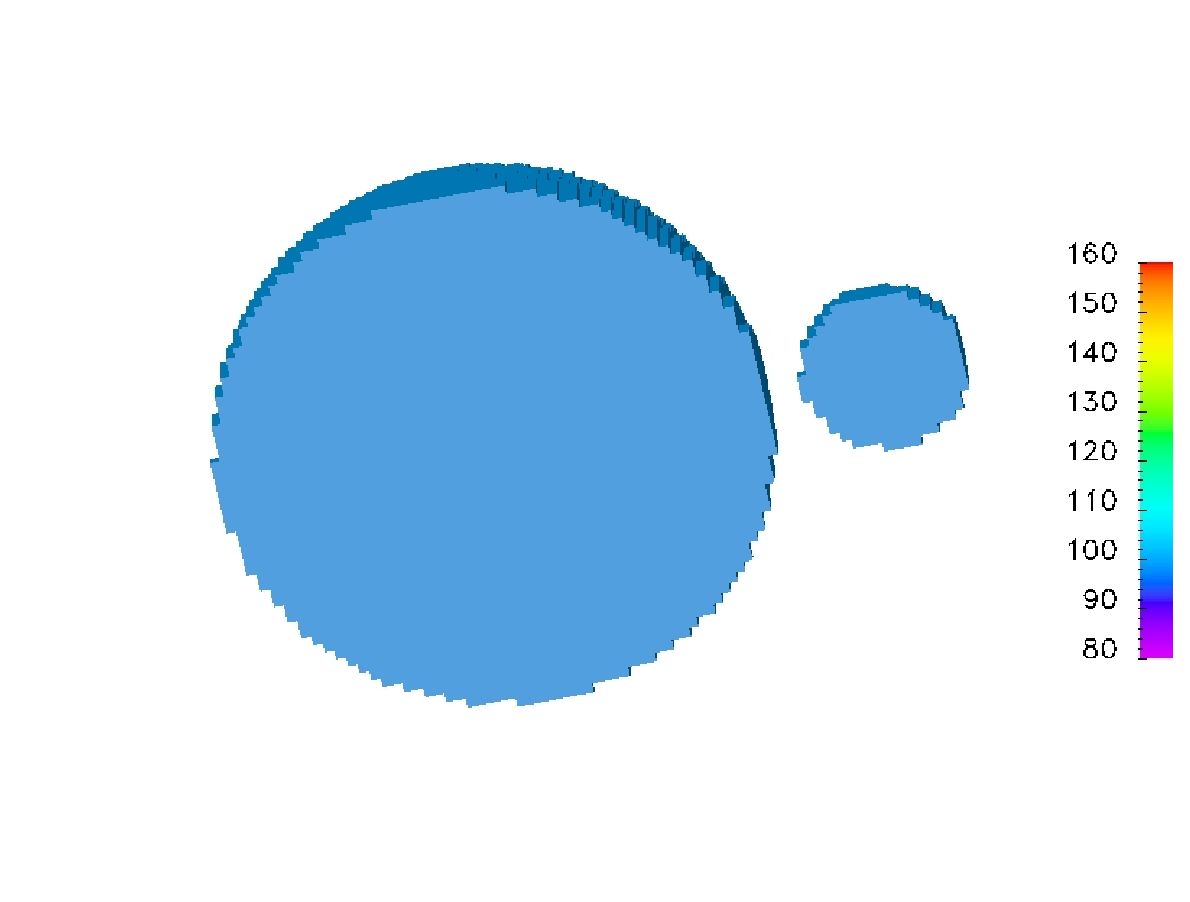
\includegraphics[scale=0.6]{b4fig1.eps}\\
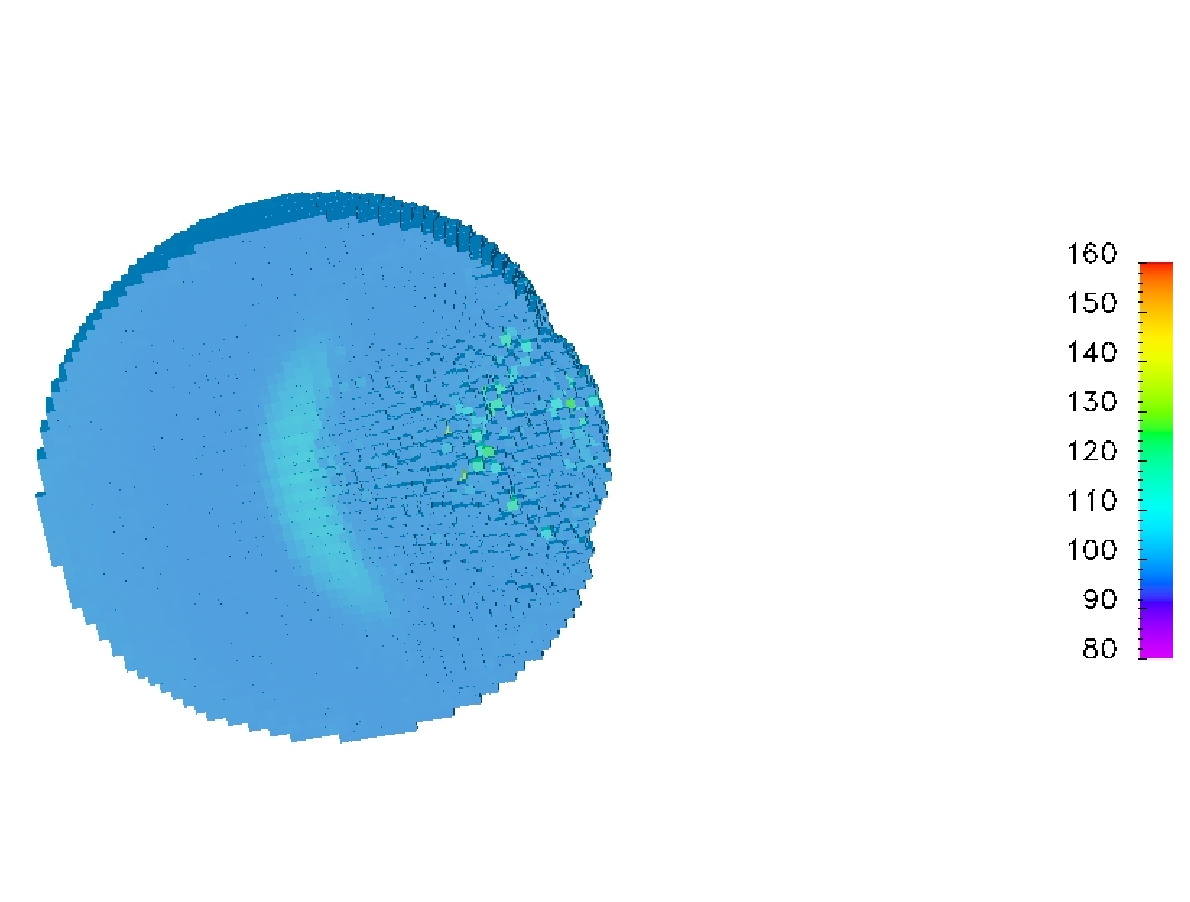
\includegraphics[scale=0.6]{b4fig2.eps} }
\caption{Simulation of an
impact: A smaller ice agglomerate impacts into a larger porous body with an
initial speed of 20~m/s. The radii of the agglomerates are 1~m and 30~cm,
respectively. The color code shows the density in units of kg/m$^3$, the
initial porosity is 0.9. In contrast to collisions between solid brittle
materials, where the impactor gets disrupted, the impacting body can enter
the target and is incorporated into it. The porosities of the target and the
impactor hardly change, and the impactor deforms plastically.}
\label{fig:b4_1}
\end{figure}
%
%
% Here follows the own refereed publications by the PIs in relation to
% the project proposed here.
%
\ownpubltitle{Own publications related to the Forschergruppe:}
%
% BELOW IS ONLY AN EXAMPLE OF TWO ENTRIES. SEE THE ADDITIONAL FILES SENT
% TO YOU WITH ALL THE REFERENCES FROM THE VORANTRAG
%
\begin{ownpubl}
\item {D'Angelo}, G., {Kley}, W. \& {Henning}, T. (2003)
   Orbital Migration and Mass Accretion of Protoplanets in
   Three-dimensional Global Computations with Nested Grids
   \apj, \textbf{586}, 540
\item de Val-Borro, M., Edgar, R.G., Artymowicz, P., Ciecielag, P.,
   Cresswell, P., D'Angelo, G., Delgado-Donate, E.J., Dirksen, G.,
   Fromang, S., Gawryszczak, A., Klahr, H., Kley, W., Lyra, W., Masset,
   F., Mellema, G., Nelson, R., Paardekooper, S.-J., Peplinski, A.,
   Pierens, A., Plewa, T., Rice, K., Sch\"afer, C., Speith, R.\ (2006)
   A comparative study of disc-planet interaction, \mn, in press
\item Ganzenm\"uller, S., Hipp, H., Kunze, S.,
Pinkenburg, S., Ritt, M., Rosenstiel, W., Ruder, H. and Sch\"afer,
C.\ (2003) Efficient and Object-Oriented Libraries for Particle Simulations, in:
\textit{High Performance Computing in Science and Engineering '03}
\item G\"unther, R., Sch\"afer, C., Kley, W.\ (2004)
   Evolution of irradiated circumbinary disks
   \aap, \textbf{423}, 559
\item Hipp, M., Pinkenburg, S., Holtwick, S., Kunze, S., Sch\"afer, C.,
Rosenstiel, W., and Ruder, H.\ (2004) Libraries and Methods for Parallel
Particle Simulations, in: \textit{High Performance Computing in Science
and Engineering '04}
\item Kley, W. \& Dirksen, G. (2006)
   Disk eccentricity and embedded planets
   \aap, \textbf{447}, 369
\item Kley, W. \& Lin, D.N.C. (1996)
   The Structure of the Boundary Layer in Protostellar Disks
   \apj, \textbf{461}, 933
\item Kley, W. \& Lin, D.N.C. (1999)
   Evolution of FU Orionis Outbursts in Protostellar Disks
   \apj, \textbf{518}, 833
\item Kley, W., {Peitz}, J. \& {Bryden}, G. (2004)
   Evolution of planetary systems in resonance
   \aap, \textbf{414}, 735
\item Kunze, S., Speith, R.~and Hessman,
F.~V.~(2001) Substantial stream-disc overflow found in three-dimensional
SPH simulations of cataclysmic variables, \mn, \textbf{322}, 499
\item Kunze, S. \& Speith. R. (2005)
   SPH Simulations of the 2:1 Resonance in Accretion Disks,
   in: \textit{The astrophysics of cataclysmic variables and related
     objects}, ASP Conf.\ Ser., {\bf 330}, 389
\item Sch{\"a}fer, C., Speith, R., G{\"u}nther, R., \& Kley, W.\ (2004a)
   Impact Simulations with SPH,
   Astronomische Nachrichten Supplement, {\bf 325}, 84
\item
Sch\"afer, C., Speith, R., Hipp, M.~and Kley, W.\ (2004b) Simulations of
planet-disc interactions using Smoothed Particle Hydrodynamics, \aap,
\textbf{418}, 325
\item Sch\"afer, C.~(2005) Application of Smooth
Particle Hydrodynamics to selected Aspects of Planet Formation, PhD
thesis, Eberhard-Karls-Universit\"at T\"ubingen
\item Speith, R.~(1998) Untersuchung von Smoothed Particle
   Hydrodynamics anhand astrophysikalischer Beispiele, PhD
thesis, Eberhard-Karls-Universit\"at T\"ubingen
\item Speith, R.~and Kley, W.~(2003) Stability of the viscously spreading ring, \aap,
\textbf{399}, 395
\end{ownpubl}
%
%
\section{Goals (Ziele)}
%

The primary goal of this project is to understand the growth of medium sized
pre-planetesimals through collisional aggregation.  For this purpose we will
use numerical models to investigate the outcome of collisions between
macroscopic dust agglomerates.  Detailed comparison between our models and
the laboratory experiments in projects \projwurm\ and \projblumtrie\ for
small ($<$ dm) agglomerates will allow both, the testing of the numerical
algorithms, as well as a deeper understanding of the phenomena observed in
the laboratory.  In the following, emphasis will be put on collisions
between particles with sizes which are too big to be used in the laboratory.
We will perform three dimensional simulations of collisions between porous
pre-planetesimals in order to study possible growth mechanisms and derive
the sticking efficiencies for various size ratios, porosities, particle
materials, and relative velocities.

\noindent
The following challenges have to be met:
%
\begin{itemize}
\item Development of a realistic model for the elastic and plastic
behavior of porous agglomerates.
\item Validation of the code by comparing the simulation results to  
the outcome of experiments.
\item Determination of the mass distribution of fragments after
collisions and the catastrophic disruption thresholds for
pre-planetesimals.
\item Study of subsequent impacts on one porous agglomerate.
\item Determination of the dust production by pre-planetesimal  
collisions.
%and possible influences on the extinction and absorption of
%protoplanetary disks.
\end{itemize}


\section{Work schedule (Arbeitsprogramm)}
%
\subsection{Methods}
%
%
The existing code will firstly be adapted to model the results of the recent
impact experiments by Wurm et al.~(2005a,b), Langkowski \& Blum (in prep.),
and Teiser \& Blum (in prep.). The Sirono model requires the knowledge of
the dependencies of the material parameters (such as the bulk and shear
moduli, the tensile, compressive and shear strengths) on the porosity. These
dependencies have been derived for ice agglomerates by Sirono~(2004). In the
case of dust agglomerates, the material parameters for some specific
porosities can be extracted from the experiments presented in Wurm et
al.~(2005a,b), Blum \& Schr\"apler~(2004), Langkowski \& Blum (in prep.),
and Teiser \& Blum (in prep.). We will fit their data to obtain the shear,
compressive and tensile strengths and the elastic properties of the dust
agglomerates for all filling factors or porosities, respectively. The best
fit data will be used to model the impact experiments by Wurm et
al.~(2005a,b), Langkowski \& Blum (in prep.) and Teiser \& Blum (in prep.),
and to compare the fragment sizes of the ejecta and the impact crater
radii. Then, the fitted values will be modified such that the results of the
simulation resemble the experimental outcome.  In this way we will acquire a
calibrated Sirono model for dust agglomerates.  In order to use a more
realistic equation of state and allow for a non-linear dependence of the
pressure on the density, the Sirono model has to be extended.

With the final (i.e.\ calibrated) code version, we intend to focus on
two-body collisions. The parameter space for the collisions between two
pre-planetesimals is tremendously wide: Size ratio of the pre-planetesimals,
collision velocity, impact angle, initial porosity, elastic and plastic
material parameters (compressive, tensile and shear strength, bulk and shear
modulus) need to be varied in order to obtain reliable statistics and cover
the uncertainties in the knowledge about the material properties of
pre-planetesimals.

The whole survey of collisions will then allow us to predict the collisional
outcome between two agglomerates with specified parameters.  The goal is to
provide, in analogy to Benz \& Asphaug (1999), the catastrophic disruption
coefficients which are basic input parameters in statistical simulations
dealing with the dust growth in the whole disk, such as coagulation
simulations of dust growth or the modeling of planetary accretion, that is
the growth from planetesimals to protoplanets and terrestrial planets (see
e.g.~Weidenschilling 2000; Dullemond \& Dominik 2004; Inaba et
al.~2001). The catastrophic disruption coefficient is the kinetic energy in
the collision divided by the target mass
%
\begin{equation} Q_\mathrm{D}= \frac{1}{2}mv^2/M, \end{equation}
%
when the collision leads to the complete disruption of the target, and
the mass of the largest remaining fragment is half the target mass.

The mass distribution of the fragments after a collision can be determined
by the complete analysis of the collisional remnants.  This is essential
input to the coagulation/fragmentation project \projdul{}, and via such
models will affect the model predictions for IR spectra of the
protoplanetary accretion disk in conjunction with project \projwolf{}.
% An important goal of
% the project will be to derive observable influences of material properties
% of the pre-planetesimals on the IR spectra of the protoplanetary accretion
% disk in conjunction with project \projwolf. 
% This can be achieved if the
% complete mass spectra of the fragments after the collision is determined and
% the production of dust grains from larger objects is known. The re-formed
% dust grains in the $\mu$m size change the IR spectra significantly. The
% results of the simulations can therefore be compared to observations of the
% SPITZER telescope (Bryden et al.~2006).
%
%----------------------------------------
\subsection{Schedule}
%
\subsubsection{First year}
%
%
Development of a realistic model for the elastic and plastic behavior of
porous agglomerates: Extension of the Sirono model and calibration of the
code. This part of the project will be tackled in very close collaboration
with J.~Blum and G.~Wurm (cf.\ Project B1-B3).  We will first use data from
their experiments as published in Blum \& Schr\"apler~(2004), Wurm et al.\
(2005a,b), Langkowski \& Blum (in prep.), and Teiser \& Blum (in prep.)  to
obtain a realistic model for the elastic properties and compressive, tensile
and shear strengths for dust agglomerates.

Dedicated impact experiments for the deduction of elastic flattening,
plasticity, onset of fragmentation and fragment mass distribution for
dust agglomerates of various sizes and porosities will be carried out
in the Braunschweig and M\"unster laboratories.

When the code will successfully reproduce the experimental
outcome, the simulations will be extended into a larger size range which
cannot be examined in the laboratory.

\subsubsection{Second year}

Determination of the catastrophic disruption thresholds for
pre-planetesimals: The main task of the project requires an immense
number of simulations in order to achieve reliable statistics.
Therefore, the setup of the simulations and the analysis of the results
have to be automated. We plan simulations involving bodies of sizes
ranging between 1~cm and 100~m.
At first, we will focus on one target and impactor material and vary
only the porosity of the target and the kinetic energy of the collision,
while all other material parameters are kept fixed, and we will focus on
collision velocities that are predicted by \projklahr. In this way, the
{\it catastrophic disruption threshold} $Q_\mathrm{D}$ can be determined
as a function of the target size and the initial porosity.  To study the
differences in oblique impacts, some of the simulations will be repeated
using different angles (e.g.\ 30 and 60 degrees) of incidence.

Study of subsequent collisions: The code will 
additionally be used to simulate the experiments which are performed in
\projwurm, that is the evolution of a large dusty body under the
influence of multiple impacts. In this way, the numerical model will be
improved continuously with more data becoming available.

\subsubsection{Third year}
%
%
Determination of the mass distribution of fragments after collisions:
The simulations demand for high
resolutions in order to resolve the fragments on the lower length scale.
The automated analysis of the simulation results includes the detection
of the fragments, their mass, momentum and angular momentum.
Accordingly, the remains of the target, especially the changes in the
form factor/shape and the porosity are recorded. The results from these
simulations will be important for the dust coagulation project \projdul\
as they provide necessary input for the coagulation equations.

Determination of the dust production by pre-planetesimal collisions:
The collisions with the most likely parameters
will be simulated at very high resolutions to investigate the dust
production by collisions between larger objects. However, it will be not
possible to resolve the fragments in the micron size range if the
initial agglomerates are meter-sized. The production of particles in the
micron size range can be predicted by the scaling of the mass
distribution of the fragments to lower sizes, though.

\subsection{Literature}
%
% Here follows a general literature list related to the topic of the
% proposal, just like a literature list for a scientific paper.
%
% AGAIN ONLY EXAMPLES ARE LISTED NOW
%
\begin{literature}
\item Ahrens, T.~J.\ and Rubin, A.~M.\ (1993) Impact-induced tensional
failure in rock, \jgr, \textbf{98}, 1185
\item Beckwith, S.~V.~W.~and Sargent, A.~I.\ (1996) Circumstellar disks
and the search for neighbouring planetary systems, \nat, \textbf{383},
129
\item Benz, W.\ (2000) Low velocity collisions and the Growth of
Planetesimals, \ssr, \textbf{92}, 279
\item Benz, W.~and Asphaug, E.\ (1994) Impact simulations with fracture.
I - Method and tests, \ica, \textbf{107}, 98
\item Benz, W.~and Asphaug, E.\ (1995) Simulations of brittle solids
using Smooth Particle Hydrodynamics, \cpc, \textbf{87}, 253
\item Benz, W.~and Asphaug, E.\ (1999) Catastrophic Disruptions
Revisited, \ica, \textbf{142}, 5
\item Blum, J.\ and Schr\"apler, R.\ (2004) Structure
and Mechanical Properties of High-Porosity Macroscopic Agglomerates
Formed by Random Ballistic Deposition, \prl, \textbf{93}, 115503
\item Blum, J.\ (2004) Grain Growth and Coagulation, in: \textit 
{Astrophysics
of Dust}, ASP Conference Series, Vol. 309 (Eds. A.~Witt, G.~Clayton and
B.~Draine), 369
\item
{Brice{\~n}o}, C., {Vivas}, A.~K., {Calvet}, N., {et~al.} (2001),
  Science, {\bf 291}, 93
%\item {Bryden}, G., {Beichman}, C.~A., {Trilling}, D.~E., {Rieke},
%G.~H., {Holmes}, E.~K., {Lawler}, S.~M., {Stapelfeldt}, K.~R., {Werner},
%M.~W., {Gautier}, T.~N., {Blaylock}, M., {Gordon}, K.~D., {Stansberry},
%J.~A.~and {Su}, K.~Y.~L.~(2006) Frequency of Debris Disks around
%Solar-Type Stars: First Results from a Spitzer MIPS Survey, {\apj},
\textbf{636},1098
\item
Dullemond, C.~P.\ and Dominik, C.~(2005) Dust coagulation in
protoplanetary disks: A rapid depletion of small grains. \aap,
\textbf{434}, 971
\item Gingold, R.~A.~and Monaghan, J.~J.~(1977) Smoothed Particle
Hydrodynamics: Theory and application to non-spherical stars, \mn,
\textbf{181}, 375
\item Grady, D.~E.~and Kipp, M.~E.~(1980) Continuum Modelling of
explosive fracture in oil shale,
\textit{Int.~J.~Rock~Mech.\ Min.~Sci.~Geomech.~Abstr.}, \textbf{17}, 147
\item Haisch, K.~E., Lada, E.~A.~and Lada, C.~J.~(2001) Disk Frequencies
and Lifetimes in Young Clusters, \apj, \textbf{553}, L153
\item Inaba, S., Tanaka, H., Nakazawa, K., Wetherill, G.~W.~and Kokubo,
E.~(2001) High-Accuracy Statistical Simulation of Planetary Accretion:
II. Comparison with N-Body Simulation, \ica, \textbf{149}, 235
\item Iveson, S.~M., Beathe, J.~A.~and Page, N.~W.~(2002) The dynamic
strength of partially saturated powder compacts: The effect of liquid
properties, \textit{Powder Techn.}, \textbf{127}, 149
\item Jutzi, M. (2004) , Diploma Thesis, University of Bern
\item Kalas, P., Graham, J.~R., Clampin, M.~C.~and Fitzgerald,
M.~P.~(2006), First scattered light images of debris disks around
HD~53143 and HD~139664, \apj, \textbf{637}, L57
\item {Kempf}, S., {Pfalzner}, S.~and {Henning}, T.~K.~(1999)
N-Particle-Simulations of Dust Growth. I. Growth Driven by Brownian
Motion, \ica, \textbf{141}, 388
\item Kendall, K., Alford, N.~McN.~and Birchall, J.~D.~(1987) A new
method for measuring the surface energy of solids, \nat, \textbf{325},
794
\item Lucy, L.~B.~(1977) A numerical approach to the testing of the
fission hypothesis, \apj, \textbf{82}, 10134
\item
{Malfait}, K., {Waelkens}, C., {Waters}, L.~B.~F.~M., {et~al.} (1998),
   \aap, {\bf 332}, L25
\item
{McCaughrean}, M.~J., {Stapelfeldt}, K.~R., \& {Close}, L.~M. (2000),
   Protostars and Planets IV, 485
\item Randles, P.~W.~and Libersky, L.~D.~(1996) Smoothed Particle
Hydrodynamics: Some recent improvements and applications,
\textit{Comp.~Methods~Appl.~Mech.~Engrg.}, \textbf{139}, 375
\item Schweiger, A~and Zimmermann, I.~(1999) A new approach for the
measurement of the tensile strength of powders, \textit{Powder Techn.},
\textbf{101}, 7
\item
{Shuping}, R.~Y., {Bally}, J., {Morris}, M., \& {Throop}, H. (2003),
   \apj, Letters, {\bf 587}, L109
\item Sirono, S.\ (2004) Conditions for collisional growth of a grain
aggregate, \ica, \textbf{167}, 431
\item Tillotson, J.~H.~(1962) Metallic equations of state for
hypervelocity impact, \textit{General Atomic Report GA-3216}
\item Voshchinnikov, V.~B.~Il'in, Henning, T.~and Dubkova, D.~N.\ (2006)
Dust extinction and absorption: The challenge of porous grains, \aap,
\textbf{445}, 167
\item Weidenschilling, S.~J.~(1977) Aerodynamics of solid bodies in the
solar nebula, \mn, \textbf{180}, 57
\item Weidenschilling, S.~J.~(1980) Dust to planetesimals - Settling and
coagulation in the solar nebula, \ica, \textbf{44}, 172
\item Weidenschilling, S.~J.~(2000) Formation of Planetesimals and
Accretion of the Terrestrial Planets, \ssr, \textbf{92}, 311
coagulation in the solar nebula, \ica, \textbf{44}, 172
\item
{Wilner}, D.~J. \& {Lay}, O.~P.~(2000), Protostars and Planets IV, 509
\item Wurm, G., Paraskov, G.~and Krauss, O.~(2005a)
Ejection of dust by elastic waves in collisions between millimeter- and
centimeter-sized dust aggregates at 16.5 to 37.5 m/s impact velocities,
\phre, \textbf{71(2)}, 021304
\item Wurm, G., Paraskov, G.~and Krauss,
O.~(2005b) Growth of planetesimals by impacts at $\sim$25 m/s, \ica,
\textbf{178}, 253
\item W{\"u}nnemann, K., Collins, G.~S., Melosh, H.~J.~(2006) A
strain-based porosity model for use in hydrocode simulations of impacts
and implications for transient crater growth in porous targets, \ica,
\textbf{180}, 514
\end{literature}



\section{External/International collaborations}
\begin{collablist}
%\item[Bern] Collaboration with the research group of Prof.~Dr.~W.~Benz
%from the University of Bern who
%is one of the leading experts in the field of SPH simulations for solid
%bodies.
\item[Nagoya] Collaboration with Dr.~S.~Sirono from the University of
Nagoya who has invented the
model for porous agglomerates that will be used for the simulations.
\item[Freiburg] Collaboration with the research group of  
Dr.~S.~Hiermaier from the
Ernst-Mach-Institut in Freiburg who is one of the leading experts in  
the field
of impact simulations.
\end{collablist}


\section{Link to other projects of the Forschergruppe}
\begin{linkproj}
\item[\projblum{}, \projwurm{} and \projblumtrie{}] The input parameters
for the simulations of the agglomerates,
e.g.~shear and tensile strengths, sound speed and shear and bulk moduli,
and especially their dependencies on the volume filling factors will  
be obtained from the projects
\projblum{}, \projwurm{} and \projblumtrie{}. Especially in the first
year, when the PhD student will calibrate the SPH code using
experimental data, the collaboration will be intensive.
\item[\projklahr{}] Project \projklahr{} provides input on the typical
impact velocities that are expected in a turbulent protoplanetary
accretion disk. Thus, the simulation survey can be restricted on the
relevant case.
\item[\projdul{}] The survey of collisions conducted in
this project includes the determination of the mass distribution of the
fragments and the catastrophic disruption coefficients which are  
needed for the dust coagulation
simulations of project \projdul{}.
% \item[\projwolf{}] The data from high resolution runs will
% give predictions on the regeneration
% of mm-sized dust particles that are observed in the (sub-)millimeter and
% infrared. Hence, the SPH simulations will provide dust production rates
% (together with the data from \projklahr\ that provides collision rates
% and probabilities) that can be used in the radiative transfer model from
% \projwolf.
\end{linkproj}



\section{Team members (Zusammensetzung der Arbeitsgruppe)}
%
% NOTE: Only list non-DFG-funded team members.
% NOTE: Also list technical assistents, students etc involved in the project
%
\begin{teamlist}
% -> Willy, some notes?
\item[Kley, W., Prof.~Dr.~(C4)]\mbox{}\\
Team leader. Supervises the PhD student funded through the project and
provides extensive expertise in computational physics and numerics.
\item[Speith, R., Dr.]\mbox{}\\
Team co-leader. Provides extensive expertise in numerical methods,
especially the Lagrangian particle method Smooth Particle
Hydrodynamics. Has widespread experience in parallel computing for
shared memory architectures using OpenMP directives and distributed
memory architectures with the Message Passing Interface (MPI).
\item[Sch\"afer, C., Dr.]\mbox{}\\
Internal collaborator. Provides extensive knowledge about the
SPH code {\tt ParaSPH} and the simulations of brittle and porous
materials.
\item[Geretshauser, R.]\mbox{}\\
Student collaborator. Code-Testing and parameter studies.
%%%%%%
%%\item[Blum, J., Prof.~Dr.~(C3)]\mbox{}\\
%%Team collaborator. Hosts the PhD student during a visit in Braunschweig
%%where the experimental setups of project \projblumtrie\ will be
%%discussed.
%%In the first year the PhD student strongly relies on the data which was
%%already measured by him and G.~Wurm in order to adopt the Sirono  
%%model to dust
%%agglomerates.
%%Specific, high temporal resolution impact experiments will be
%%performed for the calibration of the SPH code.
%%\item[Dullemond, C.~P., Dr.]\mbox{}\\
%%Team collaborator. Hosts the PhD student during a visit in Heidelberg.
%%Has excellent expertise in numerical solutions of the coagulation  
%%equations.
%%\item[Klahr, H.~H., Dr.]\mbox{}\\
%%Team collaborator. Hosts the PhD student during a visit in Heidelberg.
%%Provides excellent knowledge about the dust dynamics in turbulent
%%protoplanetary accretion disks.
%%\item[Wurm, G., Dr.]\mbox{}\\
%%Team collaborator. Hosts the PhD student during a visit in M\"unster
%%where the experimental setups of project \projwurm\ will be discussed.
%%In the first year the PhD student strongly relies on the data which was
%%already measured by him and J.~Blum in order to adopt the Sirono  
%%model to dust
%%agglomerates.
%%Specific, high temporal resolution impact experiments will be
%%performed for the calibration of the SPH code.
\end{teamlist}
\vspace{1em}



\section{Funding requested}
The following table gives the full overview of requested
funding:\vspace{1\baselineskip}\\
%
% The table that follows is the overview over the full requested
% funding, including the positions, travel, consumables and ``other
% costs'' (which might include transportation costs of radioactive
% material or the rent of a drop tower or such).
%
\centerline{\begin{tabular}{||l|r|r|r||}
\hline \hline & Year 1 & Year 2 & Year 3 \\ \hline %
Personnel (1 PhD-students: E13/2)   & \hfil 24.000 & 24.000 & 24.000 \\
Consumables                        & \hfil - & \hfil - & \hfil - \\
Travel			   	   & \hfil 2.760  & \hfil 2.500 &  \hfil 570\\ \hline
Other costs                        & \hfil 2.000 & \hfil - & \hfil - \\
\hline
{\bf Total:}                       & 28.760  & 26.500  & 24.570  \\
\hline \hline
\end{tabular}
}
\vspace{1em}\\
Below these costs are explained in more detail:

\subsection{Personnel (Personalbedarf)}
\begin{teamlist}
\item[PhD-Student 1 (E13/2)]\mbox{}\\
The PhD student will extend the porosity model and include  
experimentally
measured coefficients into the model. He/she will then perform detailed
parameter studies to determine the outcome of collision simulations.
\end{teamlist}

\subsection{Consumables (Verbrauchsmaterial)}

none

\subsection{Travel expenses in addition to Project Z (Reisekosten)}
%
% Here only travel expenses not related to usual regular Forschergruppe
% meetings and the overall per capita budget for conferences.
%
In the first year during the calibration of the model, the PhD student has
to visit Braunschweig and M\"unster for two weeks each in order to discuss
the model with J.~Blum and G.~Wurm and to participate in the experiments.
In the second year, two shorter meetings (1 week) at Braunschweig and
M\"unster are required to discuss the results of the simulations with larger
objects that are not feasible in the laboratory.  Also, the PhD student will
visit Heidelberg for two weeks for the collaboration with projects
\projklahr{}, \projdul{}. In the last year, the PhD student will
visit Heidelberg for one week to discuss the result of the simulations.

The travel costs by train to Braunschweig, Heidelberg and
M\"unster are 180~EUR, 70~EUR and 180~EUR, respectively. 
The per diem cost for food and lodging is estimated as 100 EUR per day.

Estimated costs in EUR per year:\vspace{1\baselineskip}\\
%
%
\centerline{
\begin{tabular}{||l|r|r|r||}  \hline
\hline         & Year 1   & Year 2 & Year 3 \\ \hline %
Braunschweig   &  1.380  &   680     & -    \\ \hline
Heidelberg     & -       & 1.140     &  570 \\ \hline
M\"unster      &  1.380  &   680     & -    \\
\hline \hline
{\bf Total:}   &  2.760  & 2.500     &  570 \\ \hline \hline
\end{tabular}}
%\centerline{
%\begin{tabular}{||l|l|l|l||}  \hline
%\hline         & Year 1   & Year 2 & Year 3 \\ \hline %
%%Bern           &  250  & -         &  -     \\ \hline
%Braunschweig   &  680  &  480      & -      \\ \hline
%Heidelberg     & -     & 1.140      &  570    \\ \hline
%M\"unster      &  680  &  480      &       - \\
%\hline \hline
%{\bf Total:}   & 1.360 & 2.100    &  570 \\ \hline \hline
%\end{tabular}}

\subsection{Other costs (Sonstige Kosten)}
The PhD student requires a mobile personal computer (laptop) to work
and to present his results during the visits in Braunschweig,
Heidelberg and M\"unster. The cost for this laptop (MacBook Pro) will be
approximately EUR 2000.

\section{Preconditions for carrying out the project at home institution}
%
% This is one of the main subsections of a DFG Normalverfaren proposal.
% Several of the subsubsections in this subsection we have placed in  
%their
% own subsections above (like team members, collaborations). What  
%remains
% are the following three subsections. For those not familiar with  
%these,
% we refer to the DFG Merkblatt on Normalverfahren-proposals.
%
\subsection{Scientific equipment available (Apparative Ausstattung)}
%
% Please list those larger instrument available to you for the  
%project (if
% applicable also larger computer equipment in case you need substantial
% amounts of computer time).
%
In additions to numerous individual workstations at the Institut f\"ur
Astronomie und Astrophysik, we have the following computational
equipment available
\begin{itemize}
\item Beowulf Cluster {\tt phoenix}, 16 dual AMD, IAAT
\item Beowulf Cluster {\tt pioneer}, 16 Dual Core AMD Opteron 270
with Gigabit interconnections, IAAT
\item Beowulf Cluster {\tt kepler}, 98 dual Pentium-III, 16 dual AMD
with Myrinet interconnections, SFB 382
\item Quad Itanium2 {\tt natasa}, 16 GB Memory, IAAT
\end{itemize}

Additionally, we will apply for computing time at the HLR Stuttgart
especially for the high resolution simulations. Some simulations will
also be performed on the computers available at the MPIA.


\subsection{Institution's general contribution (Laufende Mittel f\"ur  
Sachausgaben)}
%
% Please state the annual fund for consumables which comes from the
% institution's budget or any other third party  (please list  
%separately) to
% pay for the research for which your project is part of.  Use  
%estimates where
% applicable.
%
%N/A

The following table gives the general contribution from the
institution's budget:\vspace{1\baselineskip}\\
%
\centerline{\begin{tabular}{||l|r|r|r||}
\hline \hline & Year 1 & Year 2 & Year 3 \\ \hline %
Consumables                        & 500  & 500  & 500  \\
\hline
{\bf Total:}                       & 500  & 500  & 500  \\
\hline \hline
\end{tabular}
}




\cleardoublepage

\setcounter{equation}{0}
\setcounter{figure}{0}
%----------------------------------------------------------------------
%                        PROJECT DEFINITION
%----------------------------------------------------------------------
\renewcommand{\projnr}{C1}
\renewcommand{\projtitleshort}{Planetesimal precursors in turbulent disks}
\renewcommand{\projauth}{Klahr
, Kley}
%
\setcounter{section}{0}
\noindent{\normalfont\sffamily\Large\bfseries Project \projnr: \projtitleshort}
%
\section{Full title:}
\hspace{1\baselineskip}\\
\centerline{\large ``Planetesimal precursors in turbulent protoplanetary disks''}
%\centerline{\large ''}
%
\section{General information}\mbox{}
\subsection{Principle investigators:}
\hspace{-\baselineskip}\\\noindent
%
{\bfseries\itshape Klahr}, Hubertus, Dr.\\
Research Associate, non-tenure\\
Date-of-birth: 21.07.1966, Nationality: German\\
DFG Code number of latest application (KL 1469/2-1) \\
Max-Planck-Institut f\"ur Astronomie\\
K\"onigstuhl 17\\
69117 Heidelberg\\
Tel: 06221 528 255\\
Fax: 06221 528 246\\
Email: klahr@mpia.de\\
Private address: Jahnstr. 42, 67245 Lambsheim, Tel.: (06233) 50092\\
%
\vspace{1em}\\\noindent
{\bfseries\itshape Kley}, Wilhelm, Prof.~Dr.\\
Professor, tenure\\
Date-of-birth: 19. February, 1958, Nationality: German\\
DFG Code number of latest application (KL 650/7-1)\\
Institut f\"ur Astronomie \& Astrophysik\\
Abt.\ Computational Physics\\
Universit\"at T\"ubingen\\
Auf der Morgenstelle 10\\
72076 T\"ubingen\\
Tel: (07071) 29-74007\\
Fax:  (07071) 29-5094\\
Email: wilhelm.kley@uni-tuebingen.de\\
Private address: Herrenbergerstr. 73, 72070 T\"ubingen, Tel.: (07071) 640085
%

\subsection{Co-investigators within this Forschergruppe:}
\begin{coilist}
\item A.~Johansen (MPIA Heidelberg)
\item N.~Dziourkevitch (MPIA Heidelberg)
\item R.~Speith (CPT, Uni T\"ubingen)
\item D.~Marik (CPT, Uni T\"ubingen)
\end{coilist}


\section{Summary (Zusammenfassung)}
\subsubsection{Summary:} 
In this project we will use direct numerical simulations of turbulence to
study the effect on planetesimal precursors ($\approx$ 1cm - 10m). The goal
is twofold: In one part we will measure turbulent relative velocities in
high resolution local simulations, and in the other part we will determine
the global distribution of solids in the ``weather-pattern'' of turbulent
protoplanetary disks.  Thus, we can determine the key parameters for the
influence of turbulence on planetesimal formation from direct numerical
simulations.  The distribution of planetesimal precursors in the
protoplanetary disk will be derived through global 3D-MHD simulations. We
will also determine the degree to which the precursors can be concentrated
locally in protoplanetary disks in particular in flow features such as
spiral arms, high pressure regions or vortex structures.  In addition we
will derive collision speeds and probabilities as generated by the
turbulence as a function of the particle size of the collision partners and
of the location in the disk. The obtained data are an essential input for
projects B1, B2, B3 and C2, and will also be used for project D2.
%
\subsubsection{Zusammenfassung:} 
%
In diesem Projekt messen wir die Sto{\ss}raten und Geschwindigkeiten
zwi\-sch\-en felsgro{\ss}em Gesteinsmaterial im jungen solaren Nebel.  Diese
Sand bis Felsbrocken gro{\ss}en Objekte werden als das Baumaterial unserer
Planeten angesehen. In einem mittleren Gr\"o{\ss}enregime von 1 Zentimeter
bis 10 Metern Durchmesser ist turbulente Verwirbelung die Haupt\-quel\-le
f\"ur Relativgeschwindigkeiten zwischen Objekten gleicher Gr\"o{\ss}e.  Die
Turbulenz im solaren Nebel (allgemein: Protoplanetare Akkretionscheibe) wird
durch eine Magneto-Rotations-Instabilit\"at (MRI) angetrieben.  Innerhalb
des Projekts sollen die Eigenschaften solcher turbulenten Scheiben
untersucht werden und gleichzeitig die Sto{\ss}raten und Geschwindigkeiten
der eingebetteten Teilchen in Abh\"angigkeit von der Gr\"o{\ss}e der
Sto{\ss}partner und der Position in der Scheibe gemessen werden.  Diese
Messwerte k\"onnen dann direkt f\"ur die theoretischen und experimentellen
Untersuchungen von Einzelst\"o{\ss}en (siehe Projekte B1-B3) verwendet
werden und ist essentiell f\"ur Projekt C2. Sie werden auch im Project
D2 verwendet.
%
\section{State of the art (Stand der Forschung)}
%
Planets are accumulated from  micrometer-sized dust grains that are
embedded in the gas in protoplanetary disks (see Dominik et al.\ 2006 for a
recent review).  The observed infrared radiation from protoplanetary disks
comes primarily from micron-sized grains, although observations at longer
wavelengths show that some disks have large populations of grains with sizes
up to mm and cm (Rodmann et al.\ 2006). Turbulent motions in the gas play a
major role in the dynamics of chemical species and solids, at least as long
as the solids are smaller than a few decameters. Thus, an understanding of
how dust grains and chemical species move under the influence of turbulence
is vital for our understanding of the physical processes that take place in
such disks, and for the observational consequences (Ilgner 2004, Ilgner and
Nelson 2006a,b, Turner et al.\ 2006, Dullemond et al.\ 2006).

A protoplanetary disk is not turbulent a priori (see Klahr et al.~2006 for a
recent review).  Only in the presence of magnetic fields and a sufficient
ionization of the gas, an instability can develop, the magneto-rotational
instability (MRI), see Balbus \& Hawley (1991), which will lead to a state
of saturated turbulence. This turbulence is following a Kolmogorov scaling
and represents nonlinear interactions of waves in a broad spectrum.  At the
same time the turbulence develops certain short lived flow features like
vortex tubes and local pressure fluctuations. But also Coriolis forces are
important because an accretion disk is a rotating system. Thus, large enough
flow features will be in a geostrophic balance, i.e.\ magnetic and thermal
pressure are balanced by the Coriolis forces. This situation is very similar
to the weather pattern on earth.  Such geostrophic large scale features can
be very long lived (Klahr \& Bodenheimer 2003; Fromang \& Nelson 2005)
despite the action of turbulent velocity fluctuations on all smaller scales
down to the dissipation range.

Turbulence plays an important role as a driver of coagulation by causing
relative velocities between grains, in particular for particles beyond 1 mm
in size (V\"olk 1980; Mizuno 1988). The actual values of the turbulent
relative velocities used in simulations of coagulation (see Dominik et al.\
2006 for an overview) are not based on observations or numerical
simulations, but on analytical estimates similar to those of Markiewicz et
al.\ (1991). Our proposed approach to derive the quantities important for
the coagulation process from direct numerical simulations has not been
undertaken yet.
%
\subsubsection{Local Disk Simulations:}
%
In the limit of small grains (whose friction time is much shorter than an
orbital period of the disk at a given radius) the turbulence acts on the
dust purely as diffusion. The turbulent diffusion coefficient for the motion
of the grains is often assumed to be equal to the turbulent viscosity of the
gas flow (Tennekes \& Lumley 1972). Defining the {\it Schmidt number} as
the ratio between turbulent viscosity and turbulent diffusion, this
equality leads to a Schmidt number of unity.  Boosted by today's increased
computational power, and by an increased scientific interest in planet
formation and protoplanetary disks, several investigations have measured the
turbulent diffusion coefficient directly from numerical simulations of
magneto-rotational turbulence (Balbus \& Hawley 1991), the only source of
turbulence that is currently known to be consistently able to drive angular
momentum transport in gravitationally stable protoplanetary disks. The
simulations by Johansen and Klahr (2005) yield a Schmidt number that is
around unity for radial diffusion, whereas Carballido et al.\ (2005) find a
value as high as $10$.  The vertical Schmidt number, as measured both by
Johansen \& Klahr (2005), Turner et al.\ (2006) and by Fromang \&
Papaloizou (2006, gives more consistently a number between 1 and 3. Here, it
is worth to note that Turner et al.\ (2006) consider stratified disks, and
Fromang \& Papaloizou (2006) even include the effect of a dead zone without
turbulence around the mid-plane.  Recently, Johansen, Klahr \& Mee (2006)
show that the Schmidt number depends on the strength of the turbulence and
thus on the initial parameters of the disk, especially the strength of an
imposed vertical magnetic field.
%
\subsubsection{Global Disk Simulations}
%
Due to resolution and computational requirements there exist only a limited
number of global full three-dimensional magneto-hydrodynamic (3D-MHD) accretion
disk calculations.  Most of the simulations have been performed neglecting
the vertical stratification of the disk, and have used a cylindrical
potential where gravity depends only on the distance from the axis of
rotation ($z$-axis).  This setup allows the use of periodic boundary
conditions in the vertical direction and reduces the number of required
gridcells significantly.  Armitage (1998) followed the evolution of such a
global disk with a vertical seed field and obtained $\alpha$-values of the
order $10^{-1}$.  In early global simulations, Hawley (2000) has followed the
evolution of disks in a cylindrical setup and of extended equilibrium tori
with full gravity.  Simulations including diffusivity have been performed by
Arlt \& R\"udiger (2001) who use the full gravity, however in a cylindrical
coordinate system.  Due to the flaring of the disk, only a limited radial
range could be used, and the models cover only very few orbital periods
($\approx 10$).  The interaction with a surrounding atmosphere and the
generation of magnetically driven winds has been studied in 3D global
simulations by Steinacker \& Henning (2001).  Here, the disk has been
threaded by a vertical magnetic field.

In long term simulations of protoplanetary accretion disks the saturation of
the magnetic turbulence has been analyzed, using a cylindrical disk setup
without vertical gravity, by Papaloizou \& Nelson (2003).  They enclosed the
unstable region radially by an inner and outer stable layer where stability
has been achieved by using a constant azimuthal angular velocity (rigid
rotation) in these layers. This clever ``sandwich'' construction shuts off
the source of turbulence (driven by the MRI) in the inner and outer layers
and allows turbulence only in an ``active'' central region.  Using a zero
net flux condition on the magnetic field, the unstable middle region settles
after a few hundred orbital periods into a quasi-stationary state with an
effective $\alpha_{\rm eff} \approx 5 \times 10^{-3}$, which is in agreement
with standard estimates of the viscosity in protoplanetary disks.  In
follow-up simulations the evolution of massive planets embedded in such
turbulent disks have been studied (Nelson \& Papaloizou 2003), as well as
the migration of up to meter sized boulders (Fromang \& Nelson 2005). Their
simulations define presently the state of the art for ``almost'' global MHD
simulations. However, neglecting the vertical stratification of the disk
strongly limits the reliability of their results.
%
\subsubsection{Status summary}
%
The local surface density of solid material is a key parameter for
planetesimal formation. Only high enough ``dust'' surface densities will
lead to a sufficiently rapid growth of micron sized dust grains to kilometer
sized planetesimals. The same high local surface density of planetesimals is
then required to form the cores of the gas giants before the disk is
dissolved.

One possibility to accelerate the formation of planetesimals is to
concentrate the dust locally. Magneto-hydrodynamical turbulent eddies, self
gravity, spiral waves and wakes induced by existing planets will influence
the distribution of solid material and tend to create localized regions of
enhanced dust density (see Dominik et al.\ 2006).

To date there exists no comprehensive picture of how efficient these
different concentration mechanisms operate in protoplanetary disks.
Non-ideal effects (such as ionization degree, radiative cooling and
irradiative heating) and the back-reaction of the ``dust'' on the turbulence
play an important role. Not even vertical stratification has been
implemented yet in the global MHD simulations.

For the smallest dust grains the relative velocities needed for coagulation
are acquired purely by Brownian motion. For larger particles, sources of
relative velocities include differences in the settling speed and the radial
drift. But in particular for equal sized objects in the meter range still
coupled to the gas motion, turbulence induced relative velocities are the
only way that leads to collisions.

Even for very simple equations of state (isothermal configurations) there
are only very few existing simulations, most of them with no or only
approximate vertical gravity.  Here, we will focus on constructing realistic
models of radially and vertically stratified disks locally and globally, and
follow explicitly the evolution of embedded dust particles.
%
\section{Preliminary work (Eigene Vorarbeiten)}
%
In the area of local and global accretion disk simulations both research
groups at the Max-Planck Institute in Heidelberg around Hubert Klahr as well
as in the ``Computational Physics'' group in T\"ubingen (around Wilhelm
Kley) have long standing experience and excellent expertise in
multi-dimensional accretion disk simulations.
%
\subsection{Local Disk Simulations}
%
Currently, we study the diffusion properties of magneto-hydrodynamical
turbulence in {\it local} simulations of protoplanetary disks with a
restricted spatial extent (Johansen \& Klahr 2005; Johansen, Klahr \& Mee
2006).
\begin{figure}
\centering{
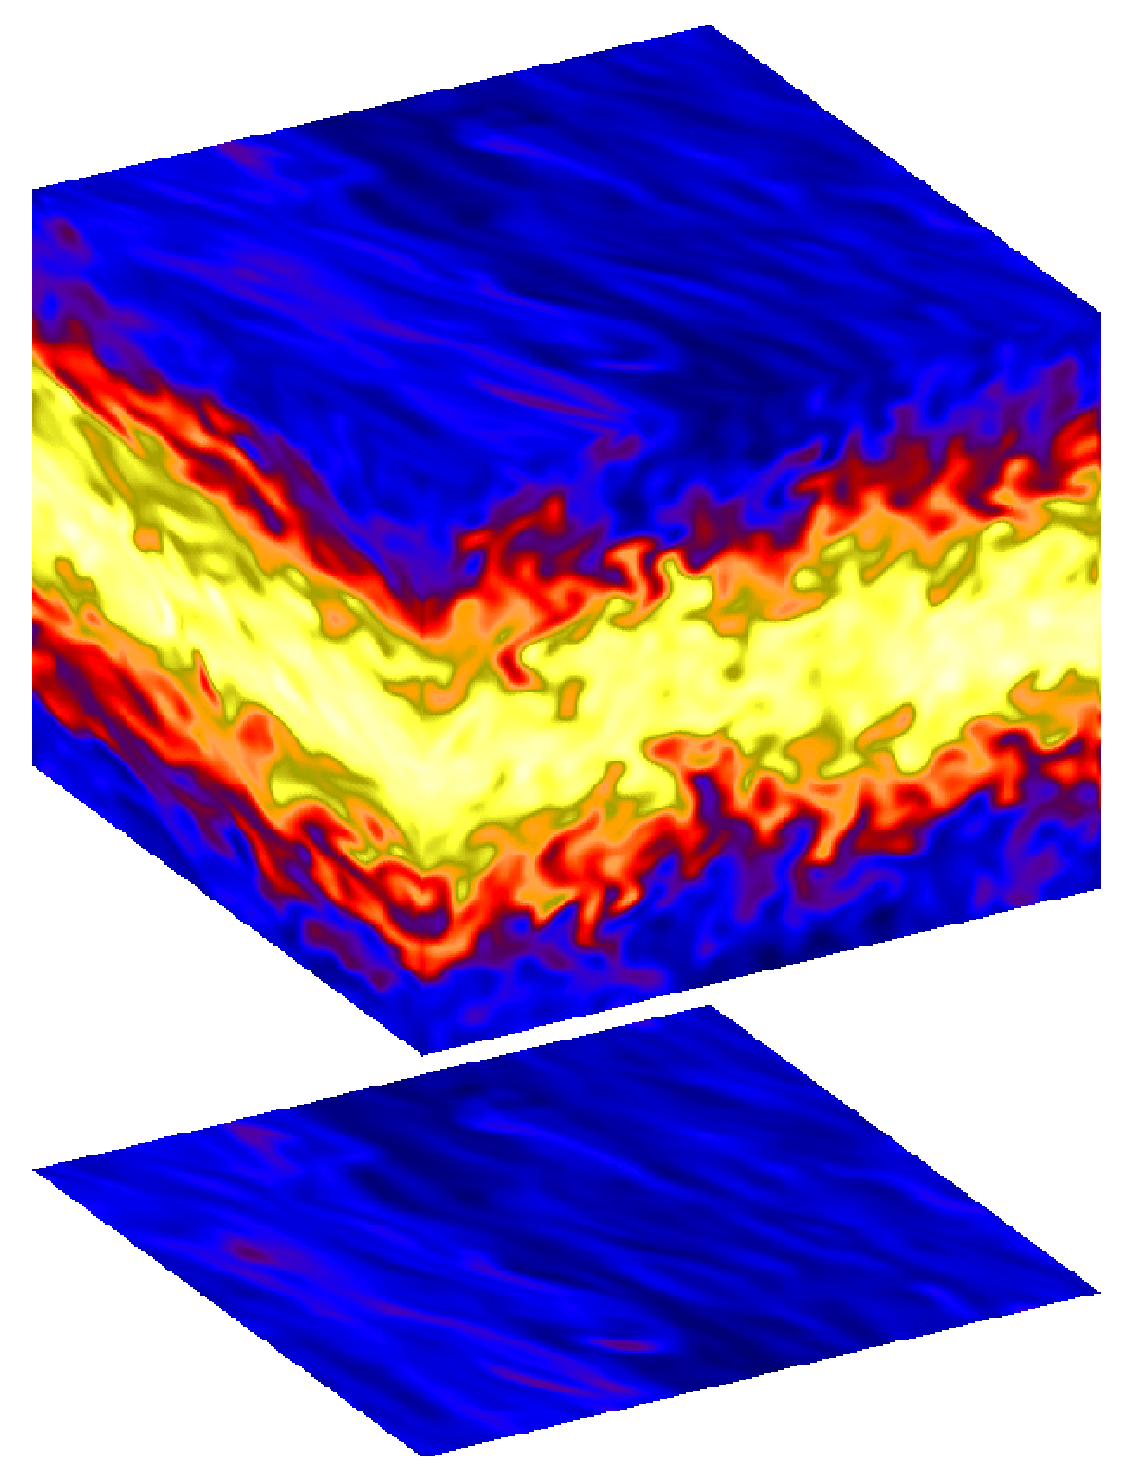
\includegraphics[scale=0.6]{c1fig1.eps}}
\caption{Particle distribution in a turbulent accretion disk. Yellow indicates
a high density around the midplane of the disk, while blue indicates the
depleted upper regions of the disk.  Here we study the equilibrium between
sedimentation and turbulent diffusion.}
\label{fig:c1_1}
\end{figure}
We measure the turbulent diffusion coefficient of dust grains embedded in
magneto-rotational turbulence in a protoplanetary disk directly from
numerical simulations and compare it to the turbulent viscosity of the
flow. The simulations are performed in a local coordinate frame comoving
with the gas which is in Keplerian rotation. Using a two-fluid approach,
small dust grains of various sizes (with friction times up to $\varOmega_0
\tau_{\rm f}=0.02$) are allowed to move under the influence of friction with
the turbulent gas. $\tau_{\rm f}$ is here the stopping time of particles due
to gas drag measured in units of the inverse Keplerian frequency
$\varOmega_0^{-1}$.  A value of $\varOmega_0 \tau_{\rm f}=0.02$ roughly
corresponds to centimeter sized particles at 5 AU in a typical solar nebula.

The turbulent diffusion coefficient of the dust grains is obtained by
applying an external sinusoidal force field acting in the vertical
direction, on the dust component only. This concentrates the dust around the
mid-plane of the disk, and an equilibrium distribution of the dust density
is achieved when the vertical settling is counteracted by the turbulent
diffusion away from the mid-plane. Comparing with analytical expressions for
the equilibrium concentration we deduce the vertical turbulent diffusion
coefficient. It is found to be lower than
the turbulent viscosity and to have an associated vertical diffusion Prandtl
number of about 1.5. A similar radial force field also allows us to measure
the radial turbulent diffusion coefficient. We find a radial diffusion
Prandtl number of about 0.85, and also find that the radial turbulent
diffusion coefficient is abound 70\% larger than the vertical. As most
angular momentum transport happens through magnetic Maxwell stresses, both
the vertical and the radial diffusion coefficients are found to be
significantly larger than suggested by the angular momentum transport due to
Reynolds stresses alone. We also find evidence for trapping of dust grains
of intermediate friction time in turbulent eddies.

We are also interested in the behavior of larger particles (with friction
times around $\varOmega_0 \tau_{\rm f}=1$), and how they are responding to
the turbulence (Johansen, Klahr and Henning 2006).  The value of
$\varOmega_0 \tau_{\rm f} = 1$ corresponds here to meter sized boulders at 5
AU in a typical solar nebula.

In this latter paper we explore the effect magneto-rotational turbulence has
on the dynamics and concentrations of boulders in local box simulations of a
sub-Keplerian protoplanetary disk.  The solids are treated as particles each
with an independent space coordinate and velocity. We find that the
turbulence has two effects on the solids: 1) Meter and decameter bodies are
strongly concentrated, locally up to a factor 100 above the average dust
density, whereas decimeter bodies only experience a moderate density
increase. The concentrations are located in large scale radial gas density
enhancements that arise from a combination of turbulence and shear.  2) For
meter-sized boulders, the concentrations cause the average radial drift
speed to be reduced by $40\%$.  We find that the densest clumps of solids
are gravitationally unstable under physically reasonable values for the gas
column density and for the dust-to-gas ratio due to sedimentation.  We
speculate that planetesimals can form in a dust layer that is not in itself
dense enough to undergo gravitational fragmentation, and that fragmentation
occurs in turbulent density fluctuations in this sub-layer.

The simulation technique we exploit for these just mentioned projects is
very similar to the methods that we plan to adopt for this proposal.  In
addition, we also have performed simulations of the Kelvin-Helmholtz
Instability in non-magnetic but stratified simulations of protoplanetary
disks (Johansen, Henning \& Klahr 2006) with a very similar
technique. Here, we also had to incorporate new physics into the code,
namely the dynamical feedback of the dust onto the gas.
%
\subsection{Global Disk Simulations}
%
Two-dimensional (2D) axisymmetric studies of {\it global} young protostellar
disks including a full stress tensor viscosity and radiative transport in
the flux-limited diffusion approximation have been applied to study the
inner boundary layer of disks (Kley \& Lin 1996), to follow the outburst of
an FU Ori system (Kley \& Lin 1999), and the convective structure of
protostellar disks has been studied in detail in (Kley et al.\ 1993). The 2D
hydrodynamical method including radiation transport has been extended by one
of the applicants (Klahr) to full three dimensions (3D) and has been used to
study the convective instability in accretion disks (Klahr et al.\ 1999).

The influence of an embedded planet on the disk structure and the
back-reaction of the disk onto the planet (migration, planetary mass
accretion) has been investigated in detail in numerous studies.  These
simulations have been performed in the pure hydrodynamic (i.e.\
non-magnetic) limit in 2D and 3D partly with nested grids (Kley 1999; Nelson
et al.\ 2000; Kley et al.\ 2001; D'Angelo et al.\ 2002; D'Angelo et al.\
2003), and with radiation transfer in 2D (D'Angelo et al.\ 2003), and
recently also in full 3D by Klahr \& Kley (2006).  In fact, many important
results defining the current status of research in the field of embedded
protoplanets have been developed by us.

Modern global accretion disk simulations rely on magneto-hydrodynamical
effects.  Within the PhD thesis of Richard G\"unther at T\"ubingen we have,
based on the Tramp-code (Klahr 1998; Klahr et al.\ 1999), recently developed
a fully parallel 3D hydrodynamical code ({\tt Tramp-MP}, G\"unther 2004).
This code has now been extended to a fully three-dimensional parallel
algorithm for solving the ideal MHD-equations (Marik et al., in prep.).  The
code is capable to solve the full system of equations in different
coordinate systems: Cartesian, cylindrical, as well as spherical polar
coordinates.  The numerical method for solving the magnetic-field evolution
is based on the constraint transport algorithm (Stone \& Norman 1992), and
all standard MHD-shock tube tests have been modeled very satisfactory.  As a
first physical application we have been able to reproduce the
magneto-rotational instability for accretion disks in the 3D global
unstratified axial case in cylindrical coordinates (Marik, Peitz \& Kley, in
preparation).  The results compare very favorably with those of Papaloizou
\& Nelson (2003), a sample snapshot of the vertically averaged density is
displayed in Fig.~\ref{fig:c1_2}.  Presently, 3D global accretion disk
models for the general, stratified, isothermal case in disk fitted spherical
coordinates are under construction.  The code, having a very modern
architecture, is meanwhile used jointly by both groups in Heidelberg and
T\"ubingen, and has been ported successfully to a variety of hardware
platforms.
 
At the same time, using the ZEUS-MP code, global accretion disk models have
been constructed for vertically isothermal stratifications (Dziourkevitch
and Klahr 2005). Here, we study the effects of vertical stratification on
the magneto-rotational turbulence in global simulations of model accretion
disks with a modified vertical potential allowing for periodic vertical
boundaries. We find a dependence of the measured Reynolds and Maxwell
stresses on the chosen vertical pressure scale height.  We also investigate
the effect of radial density and temperature stratification on the strength
of the turbulent transport.
%
%
\begin{figure}
\centering{
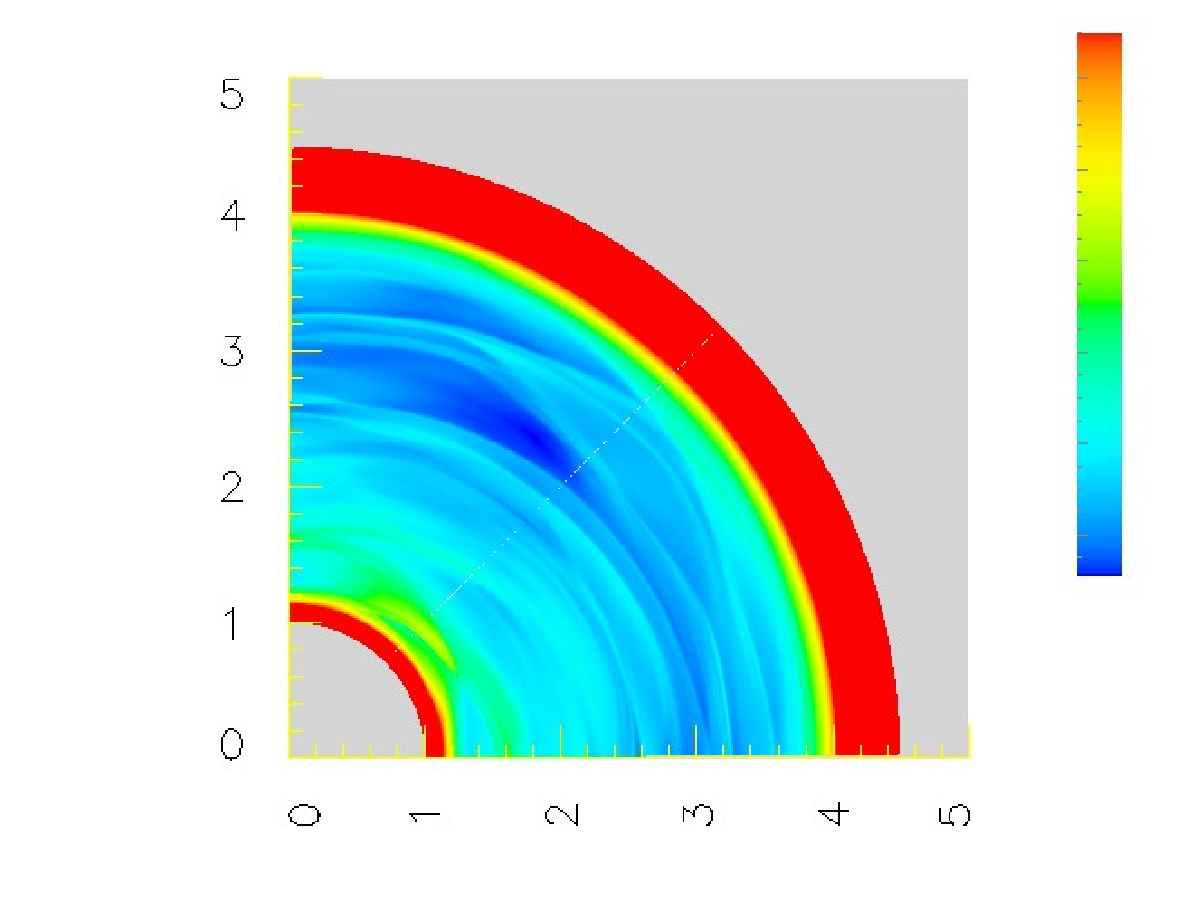
\includegraphics[scale=0.6]{c1fig2.eps}}
\caption{
Vertically averaged density for a cylindrical turbulent 3D-MHD disk using the 
newly developed code {\tt Tramp-MP}. The radial range extends from 1.0 to 4.5
in dimensionless units. At the inner and outer boundary the turbulence is
switched off by using a constant angular velocity profile, which leads to high
densities there.
}
\label{fig:c1_2}
\end{figure}

%
% Here follows the own refereed publications by the PIs in relation to
% the project proposed here.
%
\ownpubltitle{Own publications related to the Forschergruppe:}
%
% BELOW IS ONLY AN EXAMPLE OF TWO ENTRIES. SEE THE ADDITIONAL FILES 
% SENT TO YOU WITH ALL THE REFERENCES FROM THE VORANTRAG
%
\begin{ownpubl}
% CPDADD
\item Bell, K.~R., Cassen, P.~M., Klahr, H.~H. and Henning, Th. (1997) 
The Structure and Appearance of Protostellar Accretion Disks: 
Limits on Disk Flaring. \apj, \textbf{486}, 372
%
\item {D'Angelo}, G., Henning, Th. \& {Kley}, W. (2002)
  Nested-grid calculations of disk-planet interaction,
  \aap, \textbf{385}, 647
%
\item {D'Angelo}, G., Henning, Th. \& {Kley}, W. (2003)
  Thermohydrodynamics of Circumstellar Disks with High-Mass Planets,
  \aap, \textbf{599}, 548
%
\item {D'Angelo}, G., {Kley}, W. \& {Henning}, T. (2003)
  Orbital Migration and Mass Accretion of Protoplanets in
  Three-dimensional Global Computations with Nested Grids,
  \apj, \textbf{586}, 540
%
\item  Dziourkevitch, N.  \& Klahr, H. (2005)
  Global MRI in Stratified Proto-Planetary Disks, 3D Simulations,
  Protostars and Planets V, Proceedings of the 
  Conference held October 24-28, 2005 in Hawaii.
  LPI Contribution No.~1286., p.8507, 8507 
%
\item G\"unther, R. (2004)
  Three-Dimensional Parallel Hydrodynamics and Astrophysical Applications,
  Phd-thesis, Eberhard-Karls-Universit\"at T\"ubingen
%
\item Johansen, A. and Klahr, H. (2005) Dust diffusion in protoplanetary discs by
magnetorotational turbulence. \apj, \textbf{634}, 1353-1371.
%
\item Johansen, A., Klahr, H. and  Henning, Th. (2006) 
Gravoturbulent formation of planetesimals. \apj, \textbf{636}, 1121-1134.
%
\item Johansen, A., Henning, Th. and  Klahr, H. (2006) 
Dust sedimentation and self-sustained Kelvin-Helmholtz turbulence
in protoplanetary disk mid-planes. 
I. Radially symmetric simulations. \apj, in press
%
\item Johansen, A., Klahr, H. and Mee, A.J. (2006) 
Diffusion properties of magnetorotational turbulence in accretion disks:
Effects of an imposed magnetic field. \mn, in press, 
ArXiv Astrophysics e-prints arXiv:astro-ph/0603765
%
%
\item Klahr, H. and Henning, Th. (1997). 
Particle-trapping eddies in protoplanetary accretion disks,
\ica, \textbf{128}, 213--229.   % c04 - Klahr
%
\item Klahr, H. (1998)
Thermische Konvektion und Staubteilchenverteilung in protoplanetaren Akkretionsscheiben
Phd-thesis, Universit\"at Jena
%
\item Klahr, H.,  Henning, Th. \& Kley, W. (1999)
 On the Azimuthal Structure of Thermal Convection in Circumstellar Disks,
 \apj, \textbf{514}, 325
%
%CPDADD
\item Klahr, H. \& Bodenheimer, P. (2003)  Turbulence in accretion disks:
vorticity generation and angular momentum transport via the global
baroclinic instability. \apj, \textbf{582}, 869
%
\item Klahr H. \& Lin, D.~N.~C. (2005) Dust Distribution in Gas Disks II: Self 
Induced Ring Formation through a Clumping Instability. \apj, \textbf{632}, 
1113-1121.
%
%
\item Klahr,H. \& Kley, W. (2006)
 3D-radiation hydro simulations of disk-planet interactions. 
  I. Numerical algorithm and test cases,
  \aap, \textbf{445}, 747
%
\item Klahr, H. \& Bodenheimer, P.\ (2006)\ 
Formation of Giant Planets by Concurrent Accretion of Solids and Gas inside
an Anticyclonic Vortex.\ \apj, \textbf{639}, 432-440.
%
\item Klahr, H., Rozyczka, M., Dziourkevitch, N., W\"unsch, R., Johansen, A.\ 2006.\
Turbulence in Protoplanetary Accretion Disks: 
Driving Mechanisms and Role in Planet Formation.\ in  {\em Planet Formation},
Edited by Hubert Klahr and Wolfgang Brandner, pp.~.~ISBN 0521860156.~Cambridge, UK 
Cambridge University Press,  2006.\ . 
%
\item Kley, W. (1999)
  Mass flow and accretion through gaps in accretion discs,
  \mn, \textbf{303}, 696
\item Kley, W., {D'Angelo}, G., \& {Henning}, T. (2001)
  Three-dimensional Simulations of a Planet Embedded in a
   Protoplanetary Disk,
  \apj, \textbf{547}, 457
\item Kley, W. \& Lin, D.N.C. (1996)
  The Structure of the Boundary Layer in Protostellar Disks,
  \apj, \textbf{461}, 933
\item Kley, W. \& Lin, D.N.C. (1999)
  Evolution of FU Orionis Outbursts in Protostellar Disks,
  \apj, \textbf{518}, 833
\item Kley, W., Papaloizou, J.C.B. \& Lin, D.N.C. (1993)
 On the Angular Momentum Transport Associated with Convective
  Eddies in Accretion Disks,
  \apj, \textbf{416}, 679
\item Nelson, R.~P., {Papaloizou}, J.~C.~B., {Masset}, F.~S. \& Kley, W. (2000)
  The migration and growth of protoplanets in protostellar discs,
  \mn, \textbf{318}, 18
%
\item W\"unsch, R., Klahr, H.~H., and R\'o\.zyczka, M. (2005) 2-D models of layered
protoplanetary disks: I. The ring instability. \mn,  \textbf{362}, 361-368.
%
\item  W{\"u}nsch, R., Gawryszczak, A., Klahr, H., R{\'o}{\.z}yczka, M.\ (2006) 
Two-dimensional models of layered protoplanetary discs - II. The effect of a residual 
viscosity in the dead zone.\ \mn, \textbf{367}, 773-780.\
%
\end{ownpubl}
%
\section{Goals (Ziele)}
%
Within this project we plan to investigate, using {\it local and global}
numerical magnetohydro\-dynamical simulations, how the spatial distribution
and velocity distribution of dusty agglomerates within a protoplanetary disk
is affected by the turbulent motions of the gas.  The results shall be used,
in combination with the results from the experimental projects (B1, B2), to
create a coagulation kernel for the project C2.  Both, the fluctuating
collisional velocities and the fluctuating particle densities have to be
translated into an effective collision rate and sticking probability.  The
detailed fashion, how this translation can be achieved must be developed,
after we have performed the relevant direct numerical simulations.

We plan to perform complementary analysis by utilizing two different
approaches.  In Heidelberg at the Max-Planck Institut f\"ur Astronomie
(MPIA) {\it local} accretion disk simulations with embedded dust will be
performed, while at the Institute for Astronomy \& Astrophysics in
T\"ubingen (IAAT) fully {\it global} disk models will be constructed.  In
the first case we will have a higher resolution and better coverage of
statistics, while in the latter case we can focus on the global disk
effects.  This two-fold approach will enable us to obtain reliable estimates
on the statistical properties and efficiency of the MHD-turbulence in
protoplanetary accretion disks on the global as well as on the local scale,
and allow firm conclusions on the distribution of dust and boulders within
such disks.
% 
%
\begin{itemize}
\item Objective 1: {\sf Collision velocities and rates}\\
{\em Local} simulations of MHD unstable (turbulent) disks are to be
performed in Heidelberg at the MPIA, where we will treat the dust as
individual particles and follow its distribution by direct numerical
integration of the relevant equations including the interaction forces
between the gas and the dust.  As a result of the computations we will
determine the collision rates and relative velocities which play the
dominant role in the subsequent growth phase.
%
For this part of the project we will use our standard set up of local MHD
simulations. The new part will be the implementation of special measurement
tools for the individual encounter rates and velocities of the
particles. Huge amounts of data will be produced in these simulations, that
has to be interpreted with the proper statistical tools. One issue that has
to be investigated is the influence of our limited spectral range of the
turbulence on the relative velocities between the particles.  In particular,
for small particles that couple mostly to smaller length-scales than those
which are resolved one has to modify our approach of direct simulation of
turbulence. Here we plan to ``zoom'' into smaller scales of the turbulence
and neglect the larger (here unimportant) scales, but incorporate their
effect as an external forcing acting on our small box.  Settling and radial
drift can also be added, thus we will compile all the relevant local
parameters for collisions of planetesimal precursors in protoplanetary
disks.
%
\item Objective 2: {\sf Global distribution, size segregation and local
enhancement}\\ 
%
In this part of the joint project we plan to perform {\em Global} simulations
of magnetized, turbulent protoplanetary disks at the IAAT.  These
simulations will include the radial gradients (eg. differential rotation,
density and temperature profiles) in accretion disks and also a realistic
vertical stratification of the disk.  In contrast to project A2 where the
turbulence is parameterized as an effective ($\beta$-type) viscosity, we
will perform here direct numerical simulations of 3D magneto-hydrodynamical
disks. This may imply that the simulations in A2 are able to cover a larger
radial range of the disk and longer time scales, but without any azimuthal
information.
%% The two approaches can be viewed as complementary approaches.

Our new models aim towards a self-consistent treatment of turbulent disks
where the turbulent energy which is dissipated on small scales is fed back
as heat into the system, and is finally released through radiation. There
are no simulations so far in the literature that combine radiation transport
and magneto-hydrodynamics for protoplanetary disk studies.  The main
problem will consist in the combination of numerical algorithms that are
available in our two groups, and that will have to be put into a modern
computational framework and have to be parallelized.  The evolution of
embedded dust in such a fully turbulent global disk will then be followed.

\noindent
The following challenges have to be met:
%
\begin{itemize}
\item Add a module for following the evolution of embedded dust 
\item Analyze the dust distribution within the turbulence
\item Develop a parallel module for solving the radiative transport in the
 flux-limited diffusion approximation
\item Add opacities and realistic equation of state 
\item Include non-ideal effects (dissipation of kinetic and magnetic energy)
  and construct self-consistent accretion disk models
\end{itemize}

\end{itemize}
%
\section{Work schedule (Arbeitsprogramm)}
\subsection{Methods}
\subsubsection{Local Disk Simulations}
Johansen \& Klahr (2005) have performed {\em local} 3D-MHD simulations of
turbulence in accretion disks and measured the diffusion of dust induced by
the turbulence. They also studied the local concentration of meter-sized
objects in 3D-MHD turbulence by simulating $2\times 10^6$ particles
(Johansen, Klahr \& Henning 2006).  These simulations will be the starting
point for Objective 1 of this new project. The problem is very challenging
because
\begin{itemize} 
\item{particle sizes are many orders of magnitude smaller than the typical box size of such
simulations,}
\item{despite the huge number of $2\times 10^6$ particles, one is still many orders below realistic particle numbers,}
\item{and additionally the smallest scales of the turbulence can usually
not be resolved.} 
\end{itemize}
%
To overcome these obstacles we will apply two techniques: First, we will use
the concept of ``super-particles'' where one particle actually mimics an
entire flock of e.g.\ meter sized boulders, which move on a similar
path. The super-particle concept has been used successfully in plasma-physics
for many years (Birdsall \& Langdon 1985).

And second, we will perform separate simulations for the many scales of
turbulence.  Particles couple always strongest to a preferred eddy
frequency i.e.\ a certain length scale of the turbulence, where the friction
time of the particles equals the correlation time of the turbulence on that
specific scale.  This effect will give a lever to disentangle different
parts of the turbulence cascade for the relevant particle sizes.  The
strategy is to resolve not all the scales at once, but only the scales which
are important for the chosen particle size.  The effect from larger and
smaller scales can then be included via external forcing (larger scales) and
via sub-grid modeling (smaller scales).

As a final step, effects of particle growth will be included in a simplified
way, i.e.\ the individual size of the objects within a super-particle can
increase if a collision was soft enough, or decrease if the collision was
destructive.

We usually simulate the protoplanetary disk in the shearing sheet
approximation (Goldreich \& Tremaine 1978; Brandenburg et al.\ 1995; Hawley
et al.\ 1995). Here a local coordinate frame corotating with the disk with
the Keplerian rotation frequency $\varOmega_0$ at a distance $r_0$ from the
central source of gravity is considered. The coordinate system is oriented
so that $x$ points radially away from the central source of gravity, $y$
points along the Keplerian flow and $z$ points perpendicular to the disk
along the Keplerian rotation vector {\boldmath $\varOmega_0$}. As a
numerical solver we use the Pencil Code, a finite difference code that uses
sixth order symmetric space, derivatives and a third order time-stepping
scheme (see Brandenburg 2003).

The dust component is represented by typically 2,000,000 numerical particles
each with an independent position ${\bf{x}}^{(i)}$ and velocity vector ${\bf
v}^{(i)}$. The gas acts on the dust particles through a drag force that is
proportional to, but in opposite direction of, the velocity difference
between a dust grain and the surrounding gas. The equation of motion of the
dust particles is
\begin{equation}
 \frac{d {\bf v}^{(i)}}{d t} = {\bf f}({\bf v}^{(i)})
      - \frac{1}{\tau_{\rm f}} \left({\bf v}^{(i)}-{\bf u}\right) + {\bf g}\, ,
  \label{eq:eqmotp}\\
\end{equation}
where $\tau_{\rm f}$ is the {\it friction time} and $\bf{g}$ is an imposed
gravity field (see below). The term ${\bf f}({\bf v}^{(i)})$ stands for the
Coriolis forces and the shear potential necessary for the shearing sheet box
simulations (see Johansen et al.\ 2006 for a detailed definition).  In most
cases we can assume that $\tau_{\rm f}$ is a constant that is independent of
the relative velocity between the grain and the surrounding gas. In
protoplanetary disks this is a valid assumption for sufficiently small and
slow dust grains (Weidenschilling 1977). This is the case both in the
Epstein regime, where the particle is smaller than the mean free path of the
gas molecules and in the Stokes regime, where the particle is larger.  In
the Epstein regime individual collisions of the gas molecules with the grain
surface transfer the momentum, where as in the Stokes regime a laminar flow
develops around the body, producing a pressure gradient around the body. We
usually use a value of $\varOmega_0 \tau_{\rm f} < 10.0$.  Larger particles
with a more complicated aerodynamical coupling to the gas can be considered,
too. The relevant friction laws can be found in detail in Weidenschilling
(1977).

The particles change positions according to the dynamical equation
\begin{equation}
  \frac{d {\bf x}^{(i)}}{d t} = {\bf v}^{(i)} + u_y^{(0)} \hat{\bf{y}} \, .
\end{equation}
Based on these simulations we will be able to measure the desired quantities
to characterize collisions between planetesimal precursors.  Therefore, we
have to implement the measurement tools in an efficient way. The statistical
analysis tools have to be developed and simulations for various particle
sizes have to be performed, first for mono dispersive particle
distributions, and later for particle size distributions.  It will be
interesting to compare our measurements to the analytical estimations by
Markiewicz et al.~(1991), Mizuno et al.~(1988) and V\"olk et al. (1980).

We also will have to study the influence that spatial resolution has on
our results, especially as a complete coverage of the turbulent spectrum
is impossible for one single simulation. 

The master simulation is based on the models from year one. Now new models
are generated, which use only 0.1 pressure scale heights for the box size of
the computational domain instead of 1 pressure scale height in the master
model, but the identical number of grid cells.  Thus, the individual time
step is 10 times smaller, but on the other hand the relevant time scale,
e.g.\ sound crossing times and shear times are also down by a factor of
ten. The resulting total computational effort is not higher than in the
master model.  Now the resolution is 10 times better and one follows one
order of magnitude further down the turbulent cascade. The influence of the
larger scales is given by external forcing at a strength that is determined
by the master simulation. With this second simulation one can already study
what the effect of turbulence on these smaller scales has on particle
collisions in dependence of their size.

This process can be iterated for the next smaller scales by using the second
simulation as the new master simulation for the third simulation. In roughly
10 steps it will then be possible to resolve the entire cascade down to the
dissipation scale. This process has to be controlled for consistency by
e.g.\ checking the combined spectral energy distribution of the turbulence
from all the simulations. This can be compared to analytical predictions,
e.g.\ the Kolmogorov law and at least in part comparing it to spectra
obtained for high resolution simulations of turbulence. Simulations without
particles can be performed at much higher resolution, because the
computational effort is less in such a case and the simulation can also be
about 10 times shorter than in case one studies the statistical properties
of the dust.

For large particles only the largest velocities will be important, which
happen to be the largest scales, thus already resolved in the largest
box. But smaller and smaller particles couple to smaller and smaller scales
in a sense that they receive their turbulent relative (collision) velocity
only from scales, which are normally neglected in such simulations, but will
be fully covered in our project.

%
\subsubsection{Global Disk Simulations}
%
As pointed out above, even for very simple equations of state (isothermal
configurations) there are only very few existing accretion disk simulations,
most of them with no or only approximate vertical gravity.  Here, we will
focus on constructing {\it realistic models} of radially and vertically
stratified disks.

These planned {\em global} simulations of Objective 2 will be very demanding
computationally as larger physical scales and longer time-scales will have
to be covered by the calculations.  This is feasible only by utilizing very
efficient, highly parallelized codes.  Based on the existing code TRAMP
(Klahr et al.\ 1999), we have already developed a completely parallel
version {\tt Tramp-MP} which solves the 3D hydrodynamical equations
including self-gravity in arbitrary coordinates (G\"unther 2004).  The code
is based on a modern, modular algorithm written in the C++ language which
allows efficient programming using template structures and operator
overloading.  Parallelization is achieved using the library POOMA (Atlas et
al.\ 1995), which is ideally suited to develop parallel algorithms for
grid-based codes using distributed memory.  This new parallel code has been
successfully extended by us to a full 3D-MHD code that has been used to
study the Magneto Rotational Instability in isothermal global disks (Marik
et al.\ 2006, in prep.).

Within this project, efforts and expertise in Heidelberg and T\"ubingen will
be combined and the {\tt Tramp-MP}-code will extended by a by including {\it
radiative transport} in the flux-limited diffusion (FLD) approximation
similar to Klahr et al.\ (1999).  For the main part of the accretion disk
which is optically thick this approach is well justified.  At the same time
we shall implement a more realistic {\it equation of state} and {\it
opacities}, necessary for the proper radiation treatment.  To avoid too
stringent time-step limitation the radiation part will have to be solved
implicitly, which is a non-trivial task in a parallel environment. We will
base our linear equations solver on existing libraries that we utilize
already for the Poisson-solver (G\"unther 2004).  In test calculations the
newly developed module will be applied to a standard disk setup and compared
to results obtained with the 2D-code of project A2.

To obtain a self-sustained turbulent state the kinetic energy contained in
the turbulent motion has to be converted into thermal energy at the small
spatial scales. This can be achieved by including for example {\it
non-ideal} MHD-effects such as magnetic diffusion and viscosity, which
converts magnetic and kinetic energy into heat. In its present version the
code can work with either the thermal energy equation of the total
mechanical energy (thermal plus kinetic). If required to ensure better
energy conservation, the option of using a total energy equation (adding
magnetic energy) has to be considered.

In close collaboration with the first part of the project (Objective 1) we
will focus on the motion of dust in a turbulent disk.  The interaction of
the embedded dust with the flow can be incorporated in these global models
by a continuum approach by using an additional scalar field for the dust or
by explicit integration of up to currently $2 \times 10^6$ individual
particles. The important transport coefficients for the continuum approach
will be obtained from local simulations which are part of Objective 1 of
this project (see also Johansen \& Klahr 2005).

\subsection{Schedule Student 1 (located at the MPIA)}
\subsubsection{First year} 
The first goal for the student is to learn how to work with the Pencil Code
(1st three months).  The code is well documented and we have experienced
users and even developers at the MPIA. On top of that, there is an active
user group that is regularly discussing problems with the code and provides
support to each other.  The student will also have to gather experience in
the usage of the 256+8 processor computing cluster PIA and in the handling
and interpretation of the produced data.

As the initial step towards own research the student can measure relative
velocities in the existing models of turbulent disks. One has to understand
how to measure these root-mean-square velocities and how they fluctuate over
time and space (2nd three months).  In the next step these fluctuations have
to be measured and interpreted in a Lagrangian sense, i.e.\ one has to
follow the individual particles and measure the r.m.s.\ velocities and
particle densities that they experience in dependence of time.  This means
that the student has to implement suitable algorithms to efficiently measure
fluctuating collision rates, the fluctuating relative velocities and the
correlations among these values for various particle sizes.

Together with our partners in project B1, B2, B4 and especially C2 we will
discuss how to formulate a coagulation kernel from these data, especially
how our measurements compare to the analytical estimations by Markiewicz et
al.~(1991).  The experimental and numerical projects on collisions (B1, B2,
B4) will deliver critical velocities for sticking, bouncing and destruction
that have to be folded with our correlations of densities and velocities in
order to generate a coagulation kernel for C2 that only depends on the mean
particle densities and a general turbulence parameter.
 
We will then also learn what the influence of numerical parameters like
resolution and size of the computational domain are, as well as how the
effects from physical parameters like a global field strength influence our
results.  Performing the simulations for wide parameter ranges and providing
these data sets to the other groups within the Forschergruppe is the final
goal for the first year.
\subsubsection{Second year} 
Now we have to expand our local simulations of MHD turbulence in
protoplanetary disks with vertical stratification and possibly also
non-ideal MHD effects to treat an inactive mid-plane layer (four
months). The physics of e.g.\ resistivity have to be tested and verified.

The student will also develop new MHD box models that follow the turbulent
cascade down to the dissipation scale by using input (driven turbulence)
from simulations at larger scales (about four months). 


\subsubsection{Third year}
As a final goal one can now combine the MHD simulations with simulations for
the dust growth.  In that case we use the results from B1, B2 and C2 to
allow our particles to bounce, stick or destroy each other in the course of
their collisions. The small debris can feed the dust background continuum,
treated as a mass density, which is also advected.  It will also be possible
that the large bodies sweep up the small debris, thus growing in size while
depleting the back ground.  In that fashion it should be possible to let the
particles represented in the super particles grow from about 0.1 meters up
to 10 meters, which is actually the most critical part of the growth as
usually the collision velocities are too high for growth (see introduction)
as well as the radial drift rates have a maximum, which leads to a huge
particle loss towards the central object.

%%In the aftermath the student will have time
%%to write up the thesis in the last six months.

\subsection{Schedule Student 2 (located at the the University of T\"ubingen)}
\subsubsection{First year} 
In the initial phase the student has to familiarize him/herself with the
operation of the existing code {\tt Tramp-MP}. The code is well documented
and kept up to date using a CVS repository used jointly by the involved
scientists in Heidelberg and T\"ubingen.  In this first phase, the student
is expected to simulate models of global vertically stratified accretion
disks in the present code-setup using spherical polar coordinates. Here the
student will gain experience with in-output and post-processing, and
understand the internal structure and functioning of the code. By
implementing new boundary conditions on the magnetic field configurations
already new and interesting astrophysical results will be obtained.  We
estimate that this part may take about a quarter to half a year.

It will be followed by incorporation of radiative transport (flux-limited
diffusion) into the existing parallel code {\tt Tramp-MP}.  The
implementation has to be implicit which leads for a finite difference scheme
to a large system of linear equations, to be solved at each time step.  We
plan to use existing routines for example from the {\tt TIPSY} library which
have been developed particularly for MPI implementations.  The internal link
to such routines has been prepared already within the Poisson-solver routine
(G\"unther 2004). It needs to be adapted for the solution of the equations
resulting from the diffusion approximation.  The newly implemented part of
the code needs to be tested and results compared to other existing models of
(hydrodynamic) radiative disks.  This part of the project is based on our
great experience in flux-limited diffusion in 2D and 3D simulations, and
both partners in Heidelberg and T\"ubingen will actively work on this
project.  Hence, we estimate that, despite its complexities, it may take
including testing only about half a year to nine months.
%
\subsubsection{Second year} 
%
Parameter studies of fully radiative disks will be performed for different
field configurations (eg. zero net flux condition, or vertical fields).  The
statistical properties of the turbulence (total magnetic, kinetic energies,
angular momentum transport, ...) will be analyzed. We expect to arrive at
new quantitative predictions for equilibrium structures of protoplanetary
disks with respect to the magnitude of the effective $\alpha$ and its
thermal structure.

In parallel to these parameter studies we will begin with implementing a
solver to evolve the dust in such a disk. This part is based on our
experience obtained in the local simulations (at the MPIA) in which such
solvers have already been developed and used in several simulations.  We
plan to first use the continuum approach and use available results on
diffusion properties and algorithmics from the first part of the project.
For larger particle sizes the implemented particle solver from Objective 1
can be utilized.
%
\subsubsection{Third year} 
We shall perform parameter studies of global protoplanetary disks with
embedded dust.  We will analyze the statistical distribution and velocity
dispersion of the dust, and will compare results in detail with the local
runs in Objective 1.  We will examine the possibility of particle trapping
in long-lived turbulent eddies or vortices.  The possibility of rapid planet
formation through dust enhancement will be analyzed.  In case time will be
left in the project we will analyze the influence an existing planet has on
the dust distribution. In particular if this may lead to induced secondary
planet formation, and we would like to study the observational impact of an
embedded planet in a dusty disk.
%
\subsection{Literature}
%
% Here follows a general literature list related to the topic of the
% BIS HIER KAM ICH!!! HUBERT !!!
% proposal, just like a literature list for a scientific paper.
%
% AGAIN ONLY EXAMPLES ARE LISTED NOW
%
\begin{literature}
\item Arlt, R., \& R{\"u}diger, G.\ (2001) Global accretion disk simulations of 
magneto-rotational instability.\ \aap, \textbf{374}, 1035-1048. 
 
\item Armitage, P.J. (1998)
  Turbulence and Angular Momentum Transport in Global Accretion Disk Simulation
  \apj, \textbf{501}, L189
\item Atlas, S. et al., (1995)
   POOMA: A high performance distributed simulation environment for
   scientific applications, in {\it Proceedings of SuperComputing 95},
   see {\tt http://www.nongnu.org/freepooma/}
\item Balbus, S.~A., \& Hawley, J.~F. (1991) 
   A powerful local shear instability in weakly magnetized disks. I - Linear analysis,
  \apj, \textbf{376}, 214
\item Birdsall,C.K., \& Langdon, A.B., (1985) Plasma physics via computer simulation,
McGraw Hill, 1985
\item Brandenburg, A., Nordlund, A., Stein, R.~F., Torkelsson, U.\ (1995) Dynamo-generated 
Turbulence and Large-Scale Magnetic Fields in a Keplerian Shear Flow,
  \apj, \textbf{446}, 741. 
\item Brandenburg, A.\ (2003)
Computational aspects of astrophysical MHD and turbulence.\ Advances in 
Nonlinear Dynamics , \textbf{269}. 
\item Carballido A., Stone J.~M., \& Pringle J.~E. (2005) 
  Diffusion coefficient of a passive contaminant in a local MHD model of a turbulent accretion disc,
  \mn, {\bf 358}, 1055
\item  Dominik, C., Blum, J.,  Cuzzi, J., , \& Wurm, G.\ (2006) 
  Growth of Dust as the Initial Step Toward Planet Formation,
  ArXiv Astrophysics e-prints arXiv:astro-ph/0602617. 
\item Dullemond, C.~P., Apai, D., Walch, S.\ (2006) 
   Crystalline Silicates as a Probe of Disk Formation History,
   \apj {\bf 640}, L67
\item Fromang, S. \& Nelson, R.~P.\ 2005.\ On the accumulation of solid bodies in global 
turbulent protoplanetary disc models.\ \mn \textbf{364}, L81-L85. 
% 
\item Fromang, S., \& Papaloizou, J.\ (2006) Dust settling in local simulations of turbulent 
protoplanetary disks.\ ArXiv Astrophysics e-prints arXiv:astro-ph/0603153. 
%
\item Goldreich, P., \& Tremaine, S.\ 1978.\ The excitation and evolution of density waves.\ \apj, \textbf{222}, 850-858.  
%
\item Hawley, J.~F., Gammie, \& C.~F., Balbus, S.~A.\ (1995) Local Three-dimensional Magnetohydrodynamic 
Simulations of Accretion Disks, \apj, \textbf {440}, 742. 
% 
\item Hawley, J.F. (2000)
  Global Magnetohydrodynamical Simulations of Accretion Tori
  \apj, \textbf{528}, 462
\item Ilgner, M., Henning, T., Markwick, A.~J., Millar, T.~J. (2004)
   Transport processes and chemical evolution in steady accretion disk flows,
  \aap, \textbf{415}, 643
\item Ilgner, M., Nelson, R.~P.\ (2006a) On the ionisation fraction in protoplanetary disks. I. 
Comparing different reaction networks,
  \aap, \textbf{445}, 205
\item Ilgner, M., Nelson, R.~P.\ (2006b) 
  On the ionisation fraction in protoplanetary disks. II. The 
  effect of turbulent mixing on gas-phase chemistry,
  \aap, \textbf{445}, 223
\item  Johansen, A., Andersen, A.C. and Brandenburg, A. (2004). 
 Simulations of dust-trapping vortices in protoplanetary discs, 
\aap, \textbf{417}, 361--374.   % c04 - Klahr
%
\item Markiewicz, W.~J., Mizuno, H., \&Voelk, H.~J.\ (1991) Turbulence induced relative velocity 
between two grains.\ \aap \textbf{242}, 286-289. 
% 
\item Mizuno, H., Markiewicz, W.J., \& V\"olk, H.J. (1988), 
 Grain Growth in Turbulent Protoplanetary Accretion Disks, 
  \aap,  {\bf 195}, 183  % c07 - Henning
\item Nelson, R.P. \& Papaloizou, J.C.B. (2003) 
  The interaction of a giant planet with a disc with MHD turbulence -
   II. The interaction of the planet with the disc
  \mn, \textbf{339}, 993
\item Papaloizou, J.C.B. \& Nelson, R.P. (2003) 
  The interaction of a giant planet with a disc with MHD turbulence -
   I. The initial turbulent disc models
  \mn, \textbf{339}, 983
\item Rodmann, J., Henning, T., Chandler, C.~J., Mundy, L.~G., Wilner, D.~J.\ (2006) 
  Large dust particles in disks around T Tauri stars,
  \aap {\bf 446}, 211
\item Steinacker, A. \& Henning, T. (2001)
  Global Three-dimensional Magnetohydrodynamic Simulations of Accretion Disks
 and the Surrounding Magnetosphere
  \apj, \textbf{554}, 514
\item Stone, J.M. \& Norman, M.~L (1992)
  ZEUS-2D: A Radiation Magnetohydrodynamics Code for Astrophysical Flows
  in Two Space Dimensions. II. The Magnetohydrodynamic Algorithms and Tests
  \apjs, \textbf{80}, 791
%
\item Tennekes, H., \& Lumley, J.~L. (1972) First Course in Turbulence
      (Cambridge: MIT Press, 1972)
\item Turner, N.~J., Willacy, K., Bryden, G., Yorke, H.~W. (2006)
   Turbulent Mixing in the Outer Solar Nebula,
  \apj,  {\bf 639}, 1218
\item V\"olk, H.J., Jones, F.C., Morfill, G.E., \& R\"oser, S. (1980),
  Collisions between Grains in a Turbulent Gas, 
  \aap, {\bf 85}, 316   % c07 - Henning
%
\item Weidenschilling, S.~J.\ (1977) Aerodynamics of solid bodies in the solar nebula,
  \mn, {\bf 180}, 57-70. 
%
\end{literature}
%
\section{External/International collaborations}
\begin{collablist}
\item[London] We will work with Richard Nelson (QMUL) on turbulent MHD disks and particle-gas interaction.
\item[Paris] We work together with Steve Balbus on non ideal effects in accretion disks.
\item[Pasadena] We have ongoing collaborations with Neal Turner and Geoff Bryden
on Radiation Magnetohydro Simulations of Accretion disks, where we share code and experience.
\item[Potsdam] We will work with the group of Udo Ziegler on numerical MHD.
\item[Prague] Richard Wunsch is also part of the TRAMP developer and user team for
  global simulations of global accretion disks.
\item[Santa Cruz] Here we study with Doug Lin the dust distribution in optical thin but gaseous disks
with analytic and numerical methods. We also study the influence
of local dust enhancement on the core accretion model for planet formation together with Peter Bodenheimer.
\end{collablist}
%
%
\section{Link to other projects of the Forschergruppe}
\begin{linkproj}
\item[\projtscharn{}] Exchange ideas and numerical expertise concerning the
the energy transport via radiation. Define a joint test problem involving a
standard disk setup.
\item[\blockimpact{}] The derived collision velocities and rates will be
used as input and parameter guideline for the setup in
collision experiments (B1-B3, Wurm, Blum, Trieloff), and also for
the initial conditions in the numerical simulations (B4, Kley \& Speith).
On return we will use their results on the probabilities for sticking,
bouncing and destructive collisions in dependence of velocity to
fold these values with our measured velocities. 
%
\item[\projdul{}] The collision rates and velocities will be vital input for
the description of the particle growth via a coagulation equation approach.
The statistical description of the inhomogeneities, e.g.\ an intelligent
integral of the fluctuating values will be used to generate a coagulation kernel.
This kernel can then be
used in project \projdul{} to model coagulation globally in space and time.
%
\item[\projtrie{}] Predictions of the speed with which planetesimals form
(dominated by the bottle neck at 1 meter in size)
can be compared to the formation times scales of planetary cores
as obtained from radiometric dating (project \projtrie{}).
%
\item[\projwolf{}] Predictions of inhomogeneities of the dust
distribution due to particle trapping, in particular cm-sized pebbles in the
outer regions of disks, will be used in project \projwolf{} to test the
observability of such particle trapping mechanisms.
%Predictions of where in the disk, and how often, meter
%sized bodies collide and produce observable dust will be used by project
%\projwolf{}.
\end{linkproj}
%
\section{Team members (Zusammensetzung der Arbeitsgruppe)}
%
% NOTE: Only list non-DFG-funded team members.
% NOTE: Also list technical assistants, students etc involved in the project
%
\begin{teamlist}
% -> Willy, some notes?
\item[Klahr, H.~H., Dr.]\mbox{}\\
Team leader. Supervises the first PhD student at the MPIA which is
not funded through the project.
Provides excellent knowledge about the dust dynamics in turbulent
protoplanetary accretion disks.
\item[Kley, W., Prof.~Dr.~(C4)]\mbox{}\\
Team leader. Supervises the PhD student in T\"ubingen
funded through the project. Provides extensive expertise in
theory of accretion disks, planet formation, computational astrophysics
and numerical aspects.
\item[Johansen, A., PhD student]\mbox{}\\
Internal collaborator. Provides extensive knowledge about local
3D MHD calculations using the {\tt Pencil} code, including the
motion of embedded dust particles.
\item[Dziourkevitch, N., Postdoc]\mbox{}\\
Internal collaborator. Provides extensive knowledge about
3D MHD calculations using the {\tt ZEUS-MP} code, including 
non-ideal MHD effects.
\item[Marik, D., Postdoc]\mbox{}\\
Internal collaborator. Provides extensive knowledge about
3D MHD calculations using the {\tt Tramp-MP} code.
\item[Hofrichter, C., Student]\mbox{}\\
Internal collaborator. Provides extensive knowledge about
programming issues using C++ and the {\tt Tramp-MP} code..
\item[Speith, R., Dr.]\mbox{}\\
Internal collaborator. Provides extensive expertise in numerical particle methods.
Has widespread experience in parallel computing for
shared memory architectures using OpenMP directives and distributed
memory architectures with the Message Passing Interface (MPI).
\end{teamlist}
\vspace{1em}
%
\section{Funding requested}
We request funding for only {\em one} of the two PhD student positions for
this project (in T\"ubingen). The second one (Heidelberg) will be financed by the host
institution (MPIA).  The following table gives the full overview of requested
funding:\vspace{1\baselineskip}\\
%
% The table that follows is the overview over the full requested 
% funding, including the positions, travel, consumables and ``other
% costs'' (which might include transportation costs of radioactive
% material or the rent of a drop tower or such).
%
\centerline{\begin{tabular}{||l|r|r|r||} \hline \hline & Year 1 & Year 2 &
Year 3 \\ \hline %
Personnel (1 PhD-students: E13/2)   & \hfil 24.000 & 24.000 & 24.000 \\
Consumables                        & \hfil 0 & \hfil 0 & \hfil 0 \\
Travel                             & \hfil 2820 & \hfil 2820 & \hfil 2820 \\
Other costs                        & \hfil 4000 & \hfil 0 & \hfil 0 \\
\hline
{\bf Total:} (EUR)                 & \hfil 26.820 & \hfil 26.820 & \hfil 26.820 \\
\hline
\hline
\end{tabular}
}
\vspace{1em}\\
Below these costs are explained in more detail:

\subsection{Personnel (Personalbedarf)}
\begin{teamlist}
\item[PhD-Student 1 (E13/2)]\mbox{}\\
The PhD student in T\"ubingen will extend the existing code {\tt Tramp-MP}
to include radiative transport and an evolution scheme for embedded dust
particles.  He/she will then perform detailed parameter studies of global
radiative disks to determine the distribution of dust in turbulent magnetized
disks disks.
\end{teamlist}
%
\subsection{Consumables (Verbrauchsmaterial)}
none
%
\subsection{Travel expenses in addition to Project Z (Reisekosten)}
%
% Here only travel expenses not related to usual regular Forschergruppe
% meetings and the overall per capita budget for conferences.
%
The project is constructed as a close collaboration between Heidelberg and
T\"ubingen, and we envision frequent visits of the students to the partner
institutes. We plan for two visits for each year and student for one week
each.  And also one trip per year for the team leaders (2 days).  For the
return trip between Heidelberg and T\"ubingen we assume 70 EUR, and a per
diem rate of 100 EUR.  Estimated costs (in EUR) per
year:\vspace{1\baselineskip}\\
\centerline{\begin{tabular}{||l|r|r|r||} \hline \hline & Year 1 & Year 2 &
Year 3 \\ \hline %
%%  \centerline{\begin{tabular}{|p{18em}|p{7em}|p{7em}|}
\hline
4 Travel between partner Institutes (students)  &  \hfil  2280    & \hfil 2280  & \hfil 2280 \\
2 Travel between partner Institutes (leaders)  &  \hfil  540    & \hfil 540  & \hfil 540 \\
\hline
\end{tabular}}
\\[0.3cm]   
%For a trip to Potsdam we assume 150 EUR travel and 100 per diem.  For the
%trips to London and Paris we assume 200 EUR travel costs and 140 EUR per
%diem.  For trips to California we assume 1000 EUR travel and 140 EUR per
%diem.
%
\subsection{Other costs (Sonstige Kosten)}
%
The PhD students in T\"ubingen in Heidelberg require mobile personal
computers (laptops) to work and to present their results during the frequent
visits in Heidelberg and at the other partner institutes.  The cost for
these laptops (MacBook Pro) will be approximately EUR 2000 each.
%
\section{Preconditions for carrying out the project at home institution}
%
% This is one of the main subsections of a DFG Normalverfaren proposal.
% Several of the subsubsections in this subsection we have placed in their
% own subsections above (like team members, collaborations). What remains
% are the following three subsections. For those not familiar with these,
% we refer to the DFG Merkblatt on Normalverfahren-proposals.
%
\subsection{Scientific equipment available (Apparative Ausstattung)}
%
% Please list those larger instrument available to you for the project (if
% applicable also larger computer equipment in case you need substantial
% amounts of computer time).
%
In additions to numerous individual workstations at the Institut f\"ur
Astronomie und Astrophysik T\"ubingen (IAAT) and at the Max-Planck Institut
f\"ur Astronomie (MPIA), we have the following computational equipment
available
%% in T\"ubingen and Heidelberg
\begin{itemize}
\item Beowulf Cluster {\tt phoenix}, 16 dual AMD, IAAT
\item Beowulf Cluster {\tt phoenix II}, 16 Dual Core AMD Opteron 270
with Gigabit interconnections, IAAT
\item Beowulf Cluster {\tt kepler}, 98 dual Pentium-III, 16 dual AMD
with Myrinet interconnections, SFB 382
\item Quad Itanium2 {\tt natasa}, 16 GB Memory, IAAT
\item Cluster {\tt PIA}, 128 Opteron dualboards, plus 2 Opteron quadboards, MPIA
\end{itemize}

Additionally, if required we will apply for computing time at the HLR
Stuttgart in particular for the high resolution simulations.
%
\subsection{Institution's general contribution (Laufende Mittel f\"ur Sachausgaben)}
%
% Please state the annual fund for consumables which comes from the
% institution's budget or any other third party  (please list separately) to
% pay for the research for which your project is part of.  Use estimates where
% applicable. 
%
Student 1 working in Heidelberg will be funded entirely by the host
institution (MPIA).

\medskip

\noindent
The following table gives the additional general contribution from the
institutions budget:\vspace{1\baselineskip}\\
\centerline{\begin{tabular}{||l|r|r|r||}
\hline \hline & Year 1 & Year 2 & Year 3 \\ \hline %
Consumables (MPIA)                 & 500  & 500  & 500  \\
Consumables (IAAT)                 & 500  & 500  & 500  \\
\hline
{\bf Total:} (EUR)                 & 1000  & 1000  & 1000  \\
\hline \hline
\end{tabular}
}


\cleardoublepage

\setcounter{equation}{0}
\setcounter{figure}{0}
%----------------------------------------------------------------------
%                        PROJECT DEFINITION
%----------------------------------------------------------------------
\renewcommand{\projnr}{C2}
\renewcommand{\projtitleshort}{Modeling dust coagulation}
\renewcommand{\projauth}{Dullemond, Henning}
%
\setcounter{section}{0}
\noindent{\normalfont\sffamily\Large\bfseries Project \projnr: \projtitleshort}
%
\section{Full title:}
\hspace{1\baselineskip}\\
\centerline{\large ``Modeling dust coagulation on a global scale''}
%\centerline{\large ''}
%
\section{General information}\mbox{}
\subsection{Principle investigators:}
\hspace{-\baselineskip}\\\noindent
%
{\bfseries\itshape Dullemond}, Cornelis P., Dr.\\
BAT Ib, non-tenure\\
Date-of-birth: 11 December 1970, Nationality: Dutch\\
Institute: Max-Planck-Institute for Astronomy Heidelberg\\
Street+Nr: K\"onigstuhl 17\\
PLZ+City: 69117 Heidelberg\\
Tel: +49-6221-528-395\\
Fax: +49-6221-528-246\\
Email: dullemon@mpia.de\\
Private address: A.~Rausch Str. 4, 69124 Heidelberg. Tel: 06221-7290263\\
%
\vspace{1em}\\\noindent
{\bfseries\itshape Henning}, Thomas, Prof.~Dr.\\
C4, tenure\\
Date-of-birth: April 9, 1956, Nationality: German\\
DFG Code number of latest application: He 1935/21-2\\
Institute: Max-Planck-Institute for Astronomy Heidelberg\\
Street+Nr: K\"onigstuhl 17\\
PLZ+City: 69117 Heidelberg\\
Tel: +49-6221-528-200\\
Fax: +49-6221-528-246\\
Email: henning@mpia.de\\
Private address: Philosophenweg 3, 69120 Heidelberg. \\


\subsection{Co-investigators within this Forschergruppe:}
\begin{coilist}
\item J.~Blum (IGEP, TU Braunschweig)
\item G.~Wurm (M\"unster)
\item S.~Wolf (MPIA Heidelberg)
%\item K.~Kornet (DFG Emmy Noether group at the MPIA)
%\item F.~Brauer (MPIA Heidelberg)
\end{coilist}


\section{Summary (Zusammenfassung)}
\subsubsection{Summary:} 
We will develop a global model for coagulation and fragmentation of
aggregates and dusty bodies in an evolving protoplanetary disk. Within the
Forschergruppe this project will play the role of connecting the various
projects of the Forschergruppe to each other and put them into a
comprehensive context. We will investigate how the different outcomes of
aggregate collisions (depending on aggregate binding energy, porosity, ice
mantles, and processes such as sintering and eutectic melting) affect the
evolution of the particle size distribution throughout the disk.
%, and how
%particular chemical alterations of the grains get incorporated in aggregates
%through coagulation.  
The ultimate aim is to provide a unified picture of
the process of growth from sub-micron sized particles to kilometer sized
planetesimals based for a large part on the results from the Forschergruppe.

\subsubsection{Zusammenfassung:} 
In diesem Projekt planen wir, ein globales Modell f\"ur die Koagulation und
Fragmentation von Aggregaten und Staubteilchen in einer sich entwickelnden
protoplanetaren Scheibe zu konstruieren.  Innerhalb der Forschergruppe soll
das Projekt die Ergebnisse aus verschiedenen anderen Projekten zu einem
Gesamtzusammenhang zusammen\-f\"ugen. Wir werden untersuchen, wie die
unterschiedlichen Resultate von Teilchenkollisionen die Gesamtentwicklung
der Gr\"o{\ss}enverteilung der Teilchen beeinflussen (in Abh\"angigkeit von
der Bindungsenergie, Porosit\"at, Eism\"antel und Prozessen wie Sintern
und eutektisches Schmelzen).
%, und wie sich eine spezielle chemische
%Ver\"anderung der Staubk\"orner in den Aggregaten aufgrund von Koagulation
%widerspiegelt.
Das ultimative Ziel des Projekts ist die Erstellung eines Gesamtbildes des
Wachstumsprozesses der fr\"uhen Planetenentstehung von sub-mikron gro{\ss}en
Teilchen bis hin zu km-gro{\ss}en Planetesimalen, welches zu einem
gro{\ss}en Teil auf den in dieser Forschergruppe erzielten Ergebnissen
basieren wird.

\section{State of the art (Stand der Forschung)}
\subsection{Overview}
Planetary systems form from the dusty gaseous disks surrounding most young
low mass stars. But in spite of several decades of research it remains an
open issue how this happens. The two main competing scenarios are (a) that
planets form almost instantly by gravitational fragmentation of the gaseous
disk in its very early stages (Kuiper \cit{1951}; Boss
\cit{1997}, \cit{2006}), and (b) that planets form by a lengthy aggregation
and coalescence process, starting from sub-micron sized dust particles, via
multi-km sized `planetesimals', to full-grown planets (Safronov \cit{1969};
Lissauer \cit{1993}; Nakasawa et al.~\cit{2006}). While gravitational
fragmentation may indeed play an important role in the formation of Gas
Giant Planets, there is no doubt that processes like aggregation and
coalescence have taken place in our solar system, which is most clearly
demonstrated by the existence of chondritic meteorites. And for the inner
rocky planets of our solar system there is mounting evidence that
agglomeration of planetesimals and subsequent run-away and oligarchic growth
stands at the basis of their formation (Nakasawa et al.~\cit{2006}). The
objective of this project, and indeed of the entire Forschergruppe, is to
gain a better understanding of the critical first step in this growth
process: the growth from sub-micron dust particles to multi-km sized
planetesimals. We will not only build models, but also compare to
observations (mainly through project \projwolf{}).
A number of reviews give overviews of the current status
of this field (e.g.~Beckwith, Henning \& Nakagawa \cit{2000}; Dominik et
al.~\cit{2006}).

In the stage of growth from dust to kilometer sized objects gravitational
interactions between bodies play only a minor role in the growth
process. Dust grains hit and stick due to relative velocities produced by
their interaction with the gas in the disk.  Vertical sedimentation
(Safronov \cit{1969}) and radial drift (Whipple \cit{1972}) of the dust
causes particles of different sizes to acquire different velocities, and
thus cause preferentially different-size particles to collide and form
bigger aggregates. Turbulence stirs up particles of all sizes and may cause
both equal-sized particles and unequal sized particles to collide and stick
(Mizuno, Markiewicz \& V\"olk \cit{1988}). Depending on the magnitude of the
relative velocities, such collisions can lead to sticking, compaction,
fragmentation, cratering, etc. This is the topic of the studies of
block \blockimpact{} of this Forschergruppe. 
%Exactly which of these outcomes happen,
%depends on the composition and structure of the aggregates, their relative
%velocities, charge etc.\ (see block \blockimpact{} of this Forschergruppe
%proposal). 
But how these outcomes affect the distribution of particles in the
disk is the topic of the present project.

Apart from being the source of the relative velocities required for
aggregation, the processes of sedimentation, radial drift and turbulent
mixing also transport particles throughout the disk. This means that
particles that undergo growth and/or chemical/thermal processing at one
location in the disk can move to another location in the disk and affect the
growth there (Cuzzi, Davis \& Dobrovolskis \cit{2003}; Gail et
al.~\cit{2001}). The process of growth and fragmentation at different
locations in the disk are therefore coupled. An example of this is the
combined sedimentation and growth by a particle sweeping up smaller
particles on its way down to the midplane (Safronov \cit{1969}).  This can
be an effective mode of growth which is very similar to the production of
warm rain on Earth (see e.g.~Kostinski \& Shaw \cit{2005}; Riemer \& Wexler
\cit{2005}). But while the problem of the production of warm rain in the
Earth's atmosphere is that the triggering mechanism is slow, the triggering
of such `rain showers' in protoplanetary disks is extremely fast compared to
the typical life time of such disks (Dullemond \& Dominik \cit{2005}).

Thanks to theoretical models and dedicated laboratory experiments a lot is
now known about how all of these processes work (see e.g.~review by Dominik
et al.~\cit{2006}). However, many fundamental problems remain unsolved (see
below), and the solutions may well lie in the synthesis of all these
processes acting together and influencing each other.

\subsection{Coagulation/aggregation models}
The combined problem of growth and large scale motion of particles in a disk
is a complex one. In the light of the enormous number of particles involved
($\gtrsim 10^{30}$), the use of particle size distribution functions cannot be
avoided. This leads to a complex set of integro-differential equations. In
its simplest form, and without aggregate fragmentation, it can be written as: 
\begin{equation}\label{eq-coag}
\begin{split}
\frac{\partial n(\vec x,m)}{\partial t} &= 
\int_{m_\mathrm{min}}^{m/2}
K(\vec x,m',m-m')\,n(\vec x,m')\,n(\vec x,m-m')\,dm'  \\
& -\int_{m_\mathrm{min}}^{m_{\mathrm{max}}}
K(\vec x,m',m)\,n(\vec x,m')\,n(\vec x,m)\,dm'\\
& - \nabla \cdot [n(\vec x,m) \vec v(\vec x,m)] 
+ \nabla \cdot \left[D(\vec x,m)\rho_g(\vec x)
\nabla \left( \frac{n(\vec x,m)}{\rho_g(\vec x)} \right)\right] ,
\end{split}
\end{equation}
where $m$ is the mass of the particle, $\vec x$ is spatial position, $n(\vec
x,m)$ is the particle distribution function, $\vec v(\vec x)$ is the drift
velocity relative to the gas (assumed static in this simple form of the
equations), $D(\vec x,m)$ the turbulent diffusion coefficient of the
particles within the gas, and $K(\vec x,m_1,m_2)$ the coagulation kernel for
growth, which incorporates all the physics and details of the individual
collisions (i.e.~which of the various possible collision outcomes mentioned
above will happen, and how).  The first part of the right-hand-side of
Eq.(\ref{eq-coag}), i.e.~the terms with the aggregation integrals,
represents the continuous form of the {\em Smoluchowski equation}
(Smoluchowski \cit{1916}). If fragmentation is included, various other terms
need to be added to this equation (see e.g.~Th\'ebault et al.\
\cit{2003}). The second part of Eq.(\ref{eq-coag}) represent the advection
and mixing terms. These terms depend of course also on systematic motion of
the gas, which is not included in this simplified form of the equation.

First models of grain growth based on Eq.(\ref{eq-coag}) and its
generalizations were made in the eighties (Weidenschilling \cit{1980},
\cit{1984}; Nakagawa, Nakazawa \& Hayashi~\cit{1981}), but computational
cost vastly exceeded computer capabilities at that time, resulting in
somewhat crude models. Moreover, the coagulation kernel, which plays a
decisive role in the outcome of the evolution of the dust population, was
poorly known. Currently much more is known about the
coagulation/fragmentation kernel thanks to laboratory experiments (see
review by Dominik et al.~\cit{2006} and literature overview in Projects
\projblum{} and \projwurm{}) and numerical modeling (Dominik \& Tielens
\cit{1997}; Benz \& Asphaug~\cit{1994}; Sirono \& Greenberg~\cit{2000}),
although there is still a long path ahead before a reasonable complete
picture of the coagulation/fragmentation kernel is assembled.

More recent models based on these equations are: Mizuno, Markiewicz \&
V\"olk (\cit{1988}) on turbulent coagulation in disks; Weidenschilling
(\cit{1997}) on the formation of comets in the Kuiper belt; Schmitt, Henning
\& Mucha (\cit{1997}) on the feedback of coagulation on the disk evolution;
Suttner \& Yorke (\cit{2001}) on dust coagulation in the formation stages of
the disk; Dullemond \& Dominik (\cit{2005}) and Tanaka, Himeno \& Ida
(\cit{2005}) on the effect of coagulation on disk spectra, and Nomura \&
Nakagawa (\cit{2006}) on the growth of grains and the formation of a
thin unstable midplane layer.

The above papers have developed and used various algorithms for solving the
coagulation equation. A systematic study of potential numerical artifacts
from coagulation calculations was made by Ohtsuki, Nakagawa \& Nakazawa
(\cit{1990}). The problem of coagulation also plays an important role in
industry and meteorology, and in that context there is also a large volume
of literature on numerical methods of solving these equations (see
e.g.~Kraft \cit{2005} for a review).

Although models based on Eq.(\ref{eq-coag}) are necessary and useful for
studying the problem of planetesimal formation, we are very aware of the
various limitations of Eq.(\ref{eq-coag}): the simplicity of the diffusion
approximation for turbulence, the breakdown of the continuous particle
distribution approximation for run-away growth and various other problems.


\subsection{Main open questions}
Models based on Eq.~(\ref{eq-coag}) and its generalizations, require the
specification of a significant volume of input physics. The main piece of
input physics is the coagulation kernel $K(\vec x,m_1,m_2)$ and its
generalizations. Laboratory data (see projects
\projblum{}, \projwurm{} and \projblumtrie{}) as well as numerical
simulations of collisions (see project \projkley{}) give values of sticking
coefficients and fragmentation distributions for a (limited) discrete set of
initial collision conditions and initial aggregate structures. So far the
coverage of this parameter space is far from complete. High velocity impacts
have only recently been modeled (Wurm, Paraskov \& Krauss~\cit{2005}), and
the exploration of impacts of porous projectiles onto larger porous targets
have also only recently been started (Langkowski \& Blum \cit{in
prep.}). Many effects that might influence the outcome of collisions (and
are therefore part of the coagulation kernel) have as yet been
unexplored. Moreover, as part of the coagulation kernel the relative
velocities induced by turbulence (e.g.~V\"olk et al.~\cit{1980};
Weidenschilling \cit{1984}) and drift are still under debate (see project
\projklahr{}). The role of turbulence for diffusive transport, which sets
the coefficient $D(\vec x,m)$ in Eq.~(\ref{eq-coag}), is also still debated
(Johansen et al.~\cit{2005}; Carbillado, Stone \& Pringle
\cit{2005}). Uncertainties in $D(\vec x,m)$ are up to a factor of 10, which
can have major influence on the transport processes (Dullemond, Apai \&
Walch \cit{2006a}).  .

One of the main problems for aggregate growth is the `meter-size
barrier'. At 1 AU distance from the star particles of about 1 m in size have
a radial drift velocity that is so large that they drift inward to the
evaporation radius faster than they can continue to grow (Whipple
\cit{1972}; Weidenschilling \cit{1977}). Moreover, even if they do not
drift, their relative velocities are so large, that any collisions will
fragment them upon a collision (e.g.~Blum \& Wurm \cit{2000}). Various
scenarios have been suggested to `jump over' this meter-size
barrier. Goldreich \& Ward (\cit{1973}) suggested that in the absence of
turbulence the dust sediments to a very thin midplane layer which eventually
becomes gravitationally unstable and fragments into clumps which form
planetesimals. But Weidenschilling (\cit{1977}), Cuzzi, Dobrovolskis \&
Champney (\cit{1993}) and Johansen, Henning \& Klahr (\cit{2006}) have shown
that Kelvin-Helmholtz instabilities are triggered in such a layer, causing
turbulence which puffs up the layer before it becomes thin enough for
gravitational collapse. Moreover, even if such a gravitational instability
sets in, it is unclear if the collisional dissipation of kinetic
`temperature' of the swarm of particles is efficient enough for these
instabilities to produce planetesimals (e.g.~Weidenschilling
\cit{1997}). Recently, however, Youdin \& Shu (\cit{2002}) have re-examined
the problem and argued that an enhancement of solid material caused by
radial drift of particles from larger radii may help overcome these problems
(see, however, the discussion in Dominik et al.~\cit{2006}). These
scenarios, however, require zero intrinsic turbulence (i.e.~no
magneto-rotationally driven turbulence, see Balbus \& Hawley
\cit{1991}; Semenov et al.~\cit{2004}; Ilgner \& Nelson
\cit{2006}). But the observed geometric shape of protoplanetary disks
(e.g.~Burrows et al.~\cit{1996}; Throop et al.~\cit{2001}) clearly shows
that a significant amount of turbulence is present to keep the small grains
suspended in the gas. So recent new ideas to jump over the meter-size
barrier include particle concentration in vortices (e.g.~Barge \& Sommeria
\cit{1995}; Klahr \& Henning \cit{1997}), in turbulent eddies (Johansen et
al.~\cit{2006}), and in spiral waves (Rice et al.\ \cit{2004}).  Another
scenario invokes the concept of 'luck': the very few objects that happen to
survive the meter-size barrier (approx.\ 1:$10^9$) continue to grow by
sweep-up of smaller particles and eventually become planetesimals
(Weidenschilling \cit{1997}; Dullemond \& Dominik \cit{2005}). In all of the
above scenarios turbulence clearly plays a decisive role, but it is one of
the main unknowns what precisely this role is.

Once a body manages to cross the meter-size barrier, the high relative
velocities between multi-meter sized bodies and very much smaller particles
($\lesssim$ 1 cm) also poses a problem. It is, as yet, not fully clarified
whether large numbers of impacts of smaller particles on bigger objects will
cause them to grow or erode. This is, in fact, the topic of several projects
of the Forschergruppe (block B). 
%
%A large volume of research is being done at
%present to clarify this (see literature overviews in projects \projblum{}
%and \projwurm{}), but it is as yet 
%
It is as yet also unclear how these results work out on the overall size
distribution of the aggregates. It is not well known, for instance, how the
debris from such impacts affect the size distribution of the particles, how
the average structure of the aggregates/bodies changes with time
(compaction, fracturing etc), what the dominant collision partners are
(which size particle collides preferentially with which other size), and
what the main mode of growth is (ordered growth, sweep-up growth, etc.). In
addition to this, thermal processing of the grains may affect the sticking
properties of the particles (see project \projblumtrie{}), and may provide
important trace-markers for the transport of particles (see project
\projtscharn{}) which is also important to explain the mineralogical
composition of meteorites and comets and of protoplanetary disks. Charge
exchange between particles upon collisions is known in the Earth's
atmosphere to play an important role. A similar phenomenon is thought also
to play a role in disks, and might affect the sticking probability of
particles, which is still unexplored (see project \projblum{}). 
%The systematic charging of these
%particles, the movement of these charged particles throughout the disk, as
%well as the effect that the increased sticking probability has on the size
%distribution are also unexplored as yet.

Another thing which is not yet fully explored is the effect of the disk
formation process and the disk's viscous evolution on the grain size
distribution. Some work along these lines has been published by Suttner \&
Yorke (\cit{2001}) and Schmitt, Henning \& Mucha (\cit{1997}), but the time
spans of these simulations was limited.

Finally, since the recent surge of observational data from protoplanetary
disks and their dust content, a number of major new questions have arisen.
First of all, the observations in the infrared only trace the surface 
layers of the disk. The question is what the information about grain sizes
in the surface layers tells about the grain population at the midplane.
Second: observations only trace grains with sizes $\lesssim$ 1 cm, so the
question is: what does this tell about the particles $\gtrsim$ 1 cm? A third
question is: what is the cause for the observed grain sizes, and which clues
does this give to the overall aggregation process?

The present project will address many of these issues with a model of
coagulation, with input physics from projects B1, B2, B3, B4, A2 and C1,
and with output to projects D1 and D2 for comparison to measurements
of our own solar system and protoplanetary disks.

\section{Preliminary work (Eigene Vorarbeiten)}\label{sec-prelim}
\subsection{General earlier own work}
An important basis upon which coagulation models are built is a model of the
structure and evolution of the protoplanetary disk. Early models of the
disk structure were made (among others) by Bell, Cassen, Klahr \&
Henning~(\cit{1997}), Dullemond, Dominik \& Natta (\cit{2001}), Dullemond,
van Zadelhoff \& Natta (\cit{2002}) and Dullemond \& Natta
(\cit{2003a,2003b}). These were 1+1D models, i.e.\ nearly independent 1-D
vertical structure models glued together to form a 1+1D disk structure. An
improvement of that, based on 2-D radiative transfer, was developed by
Dullemond (\cit{2002}) and refined by Dullemond \& Dominik
(\cit{2004}). These models (as well as similar models from competitors) are
able to explain various observational aspects of protoplanetary disks,
including their dust emission features, the spectral energy distribution
shape, disk images etc.~(see e.g~Dullemond et al.~\cit{2006c} for a review on
disk structure models). 

Inspired by earlier work of Nakamoto \& Nakagawa (\cit{1994}) and of Hueso
\& Guillot (\cit{2005}), models were made for the time-dependent formation
and viscous evolution of protoplanetary disks (Dullemond, Apai \& Walch
\cit{2006a}). This work shows that crystalline silicates observed in such
disks may originate from the very early stages of disk formation. The same
models were also shown to be able to explain a hitherto unexplained observed
trend of accretion rate $\dot M$ with stellar mass $M_{*}$ in the Taurus and
$\rho$-Ophiuchus clusters (Dullemond, Natta \& Testi \cit{2006b}).

A crucial part of the coagulation modeling is the modeling of the motion of
particles. Schr\"apler \& Henning (\cit{2004}) studied in
detail the effect of turbulence on the sedimentation of grains to the
midplane of the disk. The effect of sedimentation on the spectra of disks
was studied by Dullemond \& Dominik (\cit{2004}).

Models of aggregation on the microscopic level were made by Kempf, Pfalzner
\& Henning (\cit{1999}) and by Ossenkopf \& Henning (\cit{1994}), which can
serve as input to the coagulation kernel. Coagulation models (based on
equations like Eq.~\ref{eq-coag}) for the very early stages of disk
evolution were presented by Schmitt, Henning \& Mucha (\cit{1997}), who also
study the back-reaction of grain growth on disk evolution. The first
comparison of a full dust coagulation model to observed spectra of
protoplanetary disks was published by Dullemond \& Dominik (\cit{2005}).
They conclude that coagulation without fragmentation is too effective in
removing small grains from the disk to be consistent with observations of
protoplanetary disks. This paper also discussed and studied a scenario of
survival of bodies through the meter-size barrier, in which a few
`lucky ones' survive the meter size barrier without a major collision,
and once they are beyond the dangerous regime, they continue to grow
by sweeping up dust.

In addition to these, the PIs have been involved in many projects which are
related to this topic: (a) Observations of spectra of dust in protoplanetary
disks (e.g.~Kessler-Silacci et al.~\cit{2006}; Apai et al.~\cit{2005};
Rodmann et al.~\cit{2006}; van Boekel et al.~\cit{2004}), (b) Radiative
transfer modeling of observations of disks (e.g.~Wolf, Henning \& Stecklum
\cit{1999}; Pontoppidan et al.~\cit{2005}), (c) Calculation of optical
properties of grains (e.g.~Henning et al.~\cit{1999}), (d) Hydrodynamics of
dusty turbulent gases (e.g.~Johansen, Klahr \& Henning \cit{2006}).



\subsubsection{Special preparations for the proposed project}\label{sec-special-prep}
The main tool for the proposed project is the aggregation/fragmentation
computer program. Currently this coagulation code is being further developed
by a PhD student (Brauer) and the PI (Dullemond) in the following three
ways, which are relevant for the proposed project:
\begin{enumerate}
\item A detailed sedimentation/mixing model is being developed for the
vertical structure of the dust of a given mass $m$. Solved are its density
structure $n(z,m)$ for a given value of $\sigma(m)\equiv \int_0^\infty
n(z,m)dz$, as well as the radial and azimuthal velocities of the gas and the
dust ($v_{g,r}(z)$, $v_{g,\phi}(z)$, $v_{d,r}(z,m)$,
$v_{d,\phi}(z,m)$). This models includes collective effects with gas-dust
friction (see Nakagawa, Sekiya \& Hayashi \cit{1986}), vertical viscosity in
both $r$ and $\phi$ velocity components (Takeuchi \& Lin \cit{2002}), and
covers both {\em given} turbulence (Dubrulle et al.~\cit{1995}) and/or {\em
self-induced} turbulence (Weidenschilling \cit{2006}). We plan to submit
this paper in the summer of 2006.
\item An implicit method of numerical solution for the combined coagulation
and fragmentation is being developed. This code will contain the numerical
algorithms, but contains only a basic coagulation/fragmentation kernel.
First version of the code is currently in the testing phase. A useable
version is expected to be ready by the end of 2006 at the latest.
\item Combining the vertical model (point 1) with the
coagulation/fragmentation code (point 2). Putting this on a time-dependent
disk formation and evolution model (Dullemond, Apai \& Walch \cit{2006a}, with
expertise input from project \projtscharn{}). 
% Include radial drift and
% radial mixing by integrating the 1-D {\em vertical} models at each radius to
% obtain vertically-integrated quantities as a function of $r$ that can be
% inserted in a 1-D {\em radial} model (see Takeuchi \& Lin \cit{2002} for an
% example of such a radial model). After one time step of disk evolution,
% radial drift and mixing, the 1-D vertical model is used to expand the model
% back to 1-D {\em vertical} models at each radius, where the coagulation can
% be computed again. 
This work is at present in the planning phase, and will likely be developed
in collaboration with the PhD student of the present proposal (see work
plan).
\end{enumerate}
Should the implicit integration turn out not to work as expected, we will
stick with our current explicit integration method and will employ parallel
computing power (which is available at the MPIA): one processor for each
vertical 1-D slab, requiring roughly 1 week for one run.

% By the start of the Forschergruppe, or at the latest after the first 6
% months of the Forschergruppe, development 1 and 2 will be ready and useable
% for the the project we propose here. At the latest during the next year (up
% to the middle of the 2nd year of the Forschergruppe) the development 3 is
% planned to be ready, but this is less essential for the project proposed
% here. Should the implicit integration turn out not to work as expected, we
% will stick with our current explicit integration method and will employ
% parallel computing power (which is available at the MPIA): one processor for
% each vertical 1-D slab, requiring roughly 1 week for one run.  {\em In any
% case, the current PhD student, F.~Brauer, will be able to provide
% substantial help and guidance to the PhD student of this proposal until
% Brauer's expected PhD defense, April 2008}. This will be of importance in
% the light of the challenging nature of the presently proposed project.




%
% Here follows the own refereed publications by the PIs in relation to
% the project proposed here.
%
\ownpubltitle{Own publications related to the Forschergruppe:}
%
% BELOW IS ONLY AN EXAMPLE OF TWO ENTRIES. SEE THE ADDITIONAL FILES 
% SENT TO YOU WITH ALL THE REFERENCES FROM THE VORANTRAG
%
\begin{ownpubl}
\item Acke, B., van den Ancker,  M.E., Dullemond, C.P., van Boekel, R. \&
  Waters, L.B.F.M. Evidence for grain growth in self-shadowed disks
  around Herbig Ae/Be stars (2004) \aap \textbf{422}, 621
\item Apai, D., Pascucci, I., Sterzik, M.F., van der Bliek, N., Bouwman, J.,
  Dullemond, C.P. \& Henning, Th. 
  Grain growth and dust settling in a brown dwarf disk: Gemini/T-ReCS
  observations of CFHT-BD-Tau 4 (2004) \aap \textbf{426}, 53
\item Apai, C.,  Pascucci, I., Bouwman, J., Natta, A., Henning, Th. \&
  Dullemond, C.P. (2005) The onset of planet formation in Brown Dwarf disks
  \sci \textbf{310}, 834
\item Bell, K.R., Cassen, P.M., Klahr, H.H. \& Henning Th. (1997)
  The Structure and Appearance of Protostellar Accretion Disks: Limits on
  Disk Flaring, \apj \textbf{486}, 372
\item Dullemond,~C.~P., Natta, A. \& Testi, L. (2006b) Accretion in
  protoplanetary disks: the imprint of core properties, \apj in press
\item {Dullemond}, C.~P. and {Apai}, D. and {Walch}, S. (2006a)
  Crystalline Silicates as a Probe of Disk Formation History, 
  \apjl \textbf{640}, 67
\item {Dullemond}, C.~P. and {Dominik}, C. (2005) Dust coagulation in
  protoplanetary disks: A rapid depletion of small grains, \aap
  \textbf{434}, 971
\item {Dullemond}, C.~P. and {Dominik}, C. (2004b) The effect of dust
  settling on the appearance of protoplanetary disks, \aap
  \textbf{421}, 1075 
\item {Dullemond}, C.~P. and {Dominik}, C. (2004a) Flaring
  vs. self-shadowed disks: The SEDs of Herbig Ae/Be stars, \aap
  \textbf{417}, 159
\item {Dullemond}, C.~P. and {Natta}, A. (2003b) An analysis of two-layer
  models for circumstellar disks, \aap \textbf{405}, 597
\item {Dullemond}, C.~P. and {Natta}, A. (2003a) The effect of scattering on
  the structure and SED of protoplanetary disks, \aap \textbf{408}, 161
\item {Dullemond}, C.~P. and {van Zadelhoff}, G.~J. and {Natta}, A.
  (2002) Vertical structure models of T Tauri and Herbig Ae/Be disks,
  \aap \textbf{389}, 464 
\item {Dullemond}, C.~P. (2002) The 2-D structure of dusty disks around
  Herbig Ae/Be stars. I.  Models with grey opacities, \aap \textbf{395}, 853
\item {Dullemond}, C.~P., {Dominik}, C. and {Natta}, A. (2001)
  Passive Irradiated Circumstellar Disks with an Inner Hole, \apj
  \textbf{560}, 957
\item Dominik, C., Dullemond, C.P., Waters, L.B.F.M.~\& Walch, S. (2003)
  Understanding the spectra of isolated Herbig stars in the frame of a passive
  disk model, \aap \textbf{398}, 607
\item Henning, Th., Il'In, V.B., Krivova, N.A., Michel, B. \& Voshchinnikov,
  N.V. (1999) WWW Database of optical constants for astronomy, 
  \aaps \textbf{136}, 405
\item Johansen, A., Klahr, H. \& Henning, Th. (2006) Gravoturbulent 
  formation of planets, \apj \textbf{636}, 1121
\item Johansen, A., Henning, Th. and  Klahr, H. (2006) 
  Dust sedimentation and self-sustained Kelvin-Helmholtz turbulence
  in protoplanetary disk mid-planes. 
  I. Radially symmetric simulations. \apj, in press
\item Kempf, S., Pfalzner, S. \& Henning, Th. (1999) N-Particle-Simulations
  of Dust Growth. I. Growth Driven by Brownian Motion, \ica \textbf{141}, 388 
\item Kessler-Silacci, J., Augereau, J.-C., Dullemond, C.P., et al. (2006)
  c2d Spitzer IRS spectra of disks around T Tauri stars. I. Silicate emission
  and grain growth, \apj \textbf{639}, 275
\item Ossenkopf, V. \& Henning, Th. (1994) Dust opacities for protostellar
  cores, \aap \textbf{291}, 943
\item Pascucci, I., Apai, D., Henning, Th.~\& Dullemond, C.~P. (2003) The
  First Detailed Look at a Brown Dwarf Disk, \apjl \textbf{590}, 111
\item Pontoppidan, K. \& Dullemond et al., C.P., (2005) Spitzer spectroscopy
  and 2D modeling of the edge-on disk CRBR 2422.8-3423 \apj \textbf{622}, 463
\item Schr\"apler, R. \& Henning, Th. (2004) Dust Diffusion, Sedimentation,
  and Gravitational Instabilities in Protoplanetary Disks, 
  \apj \textbf{614}, 960
\item Rodmann, J., Henning, Th., Chandler, C.J., Mundy, L.G. \& Wilner, D.J.
  (2006) Large dust particles in disks around T Tauri stars, 
  \aap \textbf{446}, 211
\item Schmitt, W., Henning, Th. \& Mucha, R. (1997) Dust evolution in
  protoplanetary accretion disks, \aap \textbf{325}, 569
\item van Boekel, R., Waters, L.B.F.M., Dominik, C., Bouwman, J., de Koter,
  A., Dullemond, C.P., Paresce, F. (2003) Grain growth in the inner regions of
  Herbig Ae/Be star disks, \aapl \textbf{400}, 21
\item van Boekel, R., Min, M., Leinert, Ch. et al. (2004) The building
  blocks of planets within the `terrestrial' region of protoplanetary disks,
  \nat \textbf{432}, 479
\item van Boekel, R., Waters, L.~B.~F.~M., Dominik, C., Dullemond, C.~P.,
  Tielens, A.~G.~G.~M.~\& de Koter, A. (2004) 
  Spatially and spectrally resolved 10 $\mu$m emission in
  Herbig Ae/Be stars, \aap \textbf{418}, 177
\item Wolf, S., Henning, Th. \& Stecklum (1999) Multi-dimensional
  self-consistent radiative transfer simulations based on the Monte
  Carlo method, \aap \textbf{349}, 839
\end{ownpubl}
%
%
%
%
\section{Goals (Ziele)}
The main objective is to put the various topics of the Forschergruppe into
each other's context, and thereby addressing the main objectives listed in
the `scientific objectives' of the Forschergruppe. More specifically:

%{\bf\LARGE REFORMULATE THE GOALS}
\begin{enumerate}
\item Develop a ``next-generation aggregation model'', which acts as a
unification of various projects within the Forschergruppe:
\begin{enumerate}
\item Construct realistic expressions for the coagulation kernel $K$ 
(including fragmentation, charge, porosity / fractal dimension etc.), the
turbulent particle diffusion coefficient $D$ and the average drift velocity
$v$ that go into Eq.~(\ref{eq-coag}). This will be based on the input from
various projects within the Forschergruppe (\projblum{}, \projwurm{},
\projblumtrie{}, \projkley{}, \projklahr{}, \projtscharn) and on earlier
laboratory results and computer simulations of collisions.
\item Perform simulations to discover the ways by which the various physical
processes studied by the Forschergruppe affect each other and the overall 
growth of aggregates.
\item Find out what is the relative importance of the various processes 
studied in this Forschergruppe. Which processes dominate where and when?
\item Provide feedback to the above mentioned projects: which new
experiments/simulations are needed to improve the aggregation model, and
which kind of conditions are too rare to be worthwhile to study in the
laboratory / computer simulation?
\end{enumerate}
%Special focus will be on implementing and following the effect of 
%material properties (porosity, mineralogy, ice-coatings) and grain charge 
%on the overal growth and evolution of particle distribution function.
\item Apply the code to address the following issues:
\begin{enumerate}
\item What are the time scales for the formation of planetesimals at
various positions in the disk, or for
the formation of smaller sized objects that may rapidly (by gravitational
instability) assemble to form planetesimals?
\item What is the spatial distribution of particles of various sizes, and
how does this change over time, and why?
%\item How do the various size particles influence each other? What does
%the population of small particles and their disappearance over time
%tell about the larger paticles in the disk?
%\item What are the expected compositions of asteroids and comets (having 
%incorporated materials transported to the final assembly site by various
%mechanisms)?
%\item Can large-scale charge separation take place in the disk?
\item What is the main mode of growth in various stages of the disk
life time (sweep-up, run-away, ordered)?
\item How does grain growth in the very earliest disk phases ($t\lesssim
10^5$ years), where the disk is still being formed through infalling matter
from the parent cloud, affect the grain population in the later stages? How
does the time-dependent viscous evolution of the disk affect the growth?
\item How does gradual gas removal, through e.g.~photoevaporation in the
end stages of the disk ($t\gtrsim 3\times 10^6$ years), affect the growth /
fragmentation?
\item Can big bodies like planetesimals and cometesimals form in turbulent 
disks? Observations show that disks must be at least somewhat turbulent, but
certain models rely on the absence of systematic (non-self-induced)
turbulence (e.g.~Weidenschilling \cit{1997}).
\end{enumerate}
\item In close collaboration with project \projwolf{} we will confront our
models with observations of protoplanetary disks. Two examples of such
comparisons are:
\begin{enumerate}
\item Pure grain growth would deplete the small grains much faster than is
observed (Dullemond \& Dominik~\cit{2005}, and references therein). Can
fragmentation of aggregates replenish the small dust grain population for a
sufficient amount of time?  And on which time scales do the small dust
grains eventually disappear nonetheless? Is this consistent with observed
disk dispersal rates (Haisch et al.~\cit{2001}; Carpenter~\cit{2005}), and
the formation of gaps (e.g.~Forrest et al.~\cit{2004})? And how does this
relate to the observed non-correlation between grain size-indicators and
stellar age? \label{dulgoal-smallgrains}
%\item What is the cause of the observed correlation between grain growth and
%crystallinity of grains in protoplanetary disks (van Boekel et al.~##{vBo05})?
%Can observations of crystallinity be used as a proxy of grain growth?
%\label{dulgoal-crystgrowth}
\item Recent centimeter observations of TW Hydra indicate that the large
grain population ($\sim$ 2.5 cm) is dominated by a narrow size distribution
peak (Wilner et al.~\cit{2005}). Modeling this may give clues to the binding
strength of the dust aggregates.\label{dulgoal-willner}
\end{enumerate}
In this collaboration we will also attempt to:
\begin{enumerate}
\item identify ways in which the study of observable dust grains ($a\lesssim
1$ mm) in protoplanetary disks by infrared and (sub-)millimeter telescopes
provide clues to the {\em unobservable} process of growth from $a\sim 1$ mm
to multi-kilometer planetesimals.\label{dulgoal-linkobs}
\item identify ways in which the observable grains in the {\em surface
layers} of the disk provide clues to the unobservable grains {\em deeply
embedded within the disk}.
\end{enumerate}
\end{enumerate}



\section{Work schedule (Arbeitsprogramm)}
\subsection{Methods}
\subsubsection{Available tool set}
As a basis of our project we have the following modeling tools available:
\begin{itemize}
\item Detailed disk stationary structure models in 1+1D and 2-D from 
the PI (Dullemond \cit{2002}; Dullemond et al.~\cit{2002}; Dullemond
\& Natta \cit{2003a,2003b}; Dullemond \& Dominik \cit{2004a}). A close
collaboration with the team of project A2 will also allow exchange of
expertise and algorithms on this point.
\item Time-dependent disk formation and viscous evolution models with a simple
recipe of radial mixing (Dullemond, Apai \& Walch \cit{2006}; Dullemond,
Natta \& Testi \cit{2006}).
\item A 1+1D sedimentation/aggregation/fragmentation code (Dullemond \& 
Dominik~\cit{2004b,2005}; Brauer et al.~in prep, see Section
\ref{sec-special-prep}) for modeling grain coagulation, fragmentation,
sedimentation and radial drift with size distribution functions (see Section
\ref{sec-prelim}). Two coagulation algorithms are implemented: 
the algorithm developed by Dullemond \& Dominik (\cit{2005}) as well as 
that of Kovetz \& Olund (\cit{1969}, often called the `Podolak
algorithm'). An example of the grain size distributions as a function
of time is shown in Fig.~\ref{fig-lucky}. Also on this point, a
collaboration with the project A2 will allow exchange of expertise: project
A2, while focusing on the chemistry, also needs some knowledge of grain
growth, while project C2 (this project), focusing on growth, also needs some
input on the composition of the grains.
\end{itemize}

\begin{figure}[t]
\centerline{\includegraphics[width=10cm]{c2fig1.eps}}
\caption{\label{fig-lucky}The time-dependent size distribution at the 
midplane of a disk at $r=$ 1 AU for an aggregation problem with a simple
form of fragmentation included, calculated using our methods. From
light-grey to dark grey the times are $10^{0,1,2,3,4,5}$ year respectively.
Around $t=10^4$ yr a semi-steady state sets in up to cm size. In this steady
state there is a balance between growth and destruction of aggregates. At
larger aggregate sizes there are a few `lucky ones' (about 1:10$^9$) who
have survived the fragmentation barrier (in this particular set of
parameters and input physics located at $\sim$ 10 cm) and continue to grow
by sweep up of particles from the semi-steady-state reservoir of $\lesssim$
1 cm particles. This calculation does not yet include any details of
erosion, cratering, radial drift etc.}
\end{figure}



\subsubsection{Building a realistic coagulation kernel}
For pure coagulation/aggregation without fragmentation, and for given
(known) aggregate properties as a function of mass $m$, the kernel can be
written as:
\begin{equation}\label{eq-kernel-1}
K(\vec x, m_1, m_2) = \int_0^\infty \eta(m_1,m_2,\Delta v)\;
\sigma(m_1,m_2)\; \Delta v\; P(\Delta v;\vec x,m_1,m_2)\; d \Delta v
\end{equation}
where $\sigma(m_1,m_2)$ is the collision cross-section, $\eta(m_1,m_2,\Delta
v)$ the sticking probability for particles of masses $m_1$ and $m_2$
colliding with a velocity $\Delta v$ (averaged over all possible impact
parameters), and $P(\Delta v;\vec x,m_1,m_2)$ the probability function for
the relative velocities between these particles.  Ideally one should perform
lab experiments and collision model calculations (input from projects \projblum{},
\projwurm{}, \projblumtrie{}, \projkley{}) for all combinations of $m_1$,
$m_2$ and $\Delta v$, on a fine grid in all three parameter dimensions.
Obtaining each of these values requires an averaging over all possible
impact parameters. This implies a fine-spaced scanning of a 4-D parameter
space, which is in practice impossible. The best one can obtain is a limit
set of points within this $(m_1,m_2,\Delta v)$ parameter space. To create a
smooth coagulation kernel from this, three methods can be employed: (1) a
simple semi-analytic model, (2) a simple fitting formula and (3) an
interpolation sub-routine on the measurements.

The laboratory experiments and collision models are only one factor of the
coagulation kernel. An equally important, and equally challenging, factor is
the velocity probability function $P(\Delta v;\vec x,m_1,m_2)$.  Relative
velocities caused by systematic differential drift of particles (be it
sedimentation or radial drift) produce non-disperse velocity distributions:
$P(\Delta v)=\delta(\Delta v-|\vec v_2-\vec v_1|)$. Brownian motion and
turbulence, however, produce random motions and therefore produce a
broadening of the velocity probability function. In particular for
turbulence this velocity distribution function is rather complex. An often
used simplification is to take only average relative velocities into
account. In this case the entire relative velocity probability function
$P(\Delta v)$ becomes a $\delta$-function and Eq.~(\ref{eq-kernel-1})
reduces to:
\begin{equation}\label{eq-kernel-2}
K(\vec x, m_1, m_2) = \eta(m_1,m_2,\langle\Delta v\rangle)\;
\sigma(m_1,m_2)\; \langle\Delta v\rangle
\end{equation}
The value of $\langle\Delta v\rangle$ for particles in turbulent gases have
been calculated numerically by V\"olk (\cit{1980}), Mizuno, Markiewicz \&
V\"olk (\cit{1988}), and analytic fitting formulae were derived by
Weidenschilling (\cit{1984}). But these expressions were derived under
standard assumptions for Kolmogorov turbulence. It remains unverified
whether turbulence driven by Kelvin-Helmholtz instabilities (Weidenschilling
\cit{1977}; Cuzzi et al.~\cit{1993}; Johansen \& Klahr in prep.) and/or by
magneto-rotational instability (Balbus \& Hawley \cit{1991}; Brandenburg et
al.~\cit{1996}) are of the same nature.  Moreover, it remains uncertain
whether this average-$\langle\Delta v\rangle$ approach is valid in the first
place. There are examples from meteorology in which statistical fluctuations
seem to play a major role, like in the formation of warm rain on Earth
(Kostinski \& Shaw \cit{2005}). Project \projklahr{} will play a vital role
at this point. It will provide knowledge of $P(\Delta v;\vec x,m_1,m_2)$
which is the required input here. In collaboration with that project, we
will attempt to develop fitting formulae to summarize the expected complex
functionality of $P(\Delta v;\vec x,m_1,m_2)$. We will also investigate the
importance of the above mentioned statistical fluctuations.
%  If, as hoped,
% Eq.~(\ref{eq-kernel-2}) can be used without too large problems, one of the
% tasks of project \projklahr{}, i.e.\ finding a proper expression of
% $P(\Delta v;\vec x,m_1,m_2)$, can then be reduced to finding an expression of
% $\langle\Delta v\rangle$ as a function of $\vec x$, $m_1$ and $m_2$.

The $\langle\Delta v\rangle$-approach can also introduce another problem:
for a sufficiently wide velocity distribution one could have sticking for
the lower velocity part and shattering for the higher velocity part.
Using a single $\langle\Delta v\rangle$ will ignore this effect. We will
investigate how important this effect is, and if it is important we will 
derive separate expressions for $\langle\Delta v\rangle$ for the
sticking and shattering regime.

In collaboration with project \projklahr{} we will also investigate the
effect of in homogeneities (e.g.~particle trapping) on the coagulation. 
We will develop a simple empirical `model' that describes this effect,
so that it can be built in into the coagulation code which, by its nature,
is not able to model such inhomogeneities from first principles.

\subsubsection{Implementing aggregate structure/shape effects}
In the simplest case of compact particles, one can write
$\sigma(m_1,m_2)=\pi(a_1+a_2)^2$ where $a_i=(3m/4\pi\xi)^{1/3}$ with $\xi$
the material density. This
simplifies Eq.~(\ref{eq-kernel-1}) resp.\ Eq.~(\ref{eq-kernel-2}) more.  But
aggregates are not compact particles. They can have complex structure and
can have various levels of compactness: from very tenuous fractal aggregates
(Kempf et al.~\cit{1999}; Krause \& Blum \cit{2004}) up to filling factors
of 0.33 (Blum \& Schr\"apler \cit{2004}). The outcome of collisions has been
shown to depend critically on these shape/structure parameters. It would be
impossible to model all imaginable shapes/structures. One will have to
`summarize' these properties in some kind of `shape/structure parameter',
which we call $s$ for convenience. For the sake of communication let us
assume $s$ to denote the level of `compactness'. But it can, for some
purposes, also be meant as the fractal dimension or any other structural
property that can be characterized by a single scalar.

For the laboratory experiments and collision modeling this introduces an
extra difficulty: for each $m_1$, $m_2$ and $\Delta v$, one has to do
experiments not only varying the impact parameter $b$, but also varying the
shapes, and (for non-spherical shapes) averaging over orientation and
rotation rate of the impactors. This is clearly impossible and the parameter
space of lab experiment will necessarily be sampled sparsely. In
collaboration with the various projects providing input (mainly B1, B2, B3
and B4), we will devise strategies to construct semi-analytic models and/or
fitting formulae for the full coagulation kernel based on this sparsely
sampled parameter space of experiments.

To include $s$ in the model, we should introduce it as an extra dimension in
addition to particle mass $m$:
\begin{equation}
f(\vec x,m) \rightarrow f(\vec x,m,s)
\end{equation}
which enhances the dimensionality of the aggregation problem and thereby
makes the solution more computationally expensive. As a first step we shall
avoid this by attempting to calculate an average $\langle s\rangle$ as a
function of $\vec x$ and $m$ (called $\bar s(\vec x,m)$). We will do so by
starting with a first guess for $\bar s(\vec x,m)$, constructing the
coagulation kernel for this guess (see above), and then calculating models
of aggregation. We can then determine the dominating collisions responsible
for growth by determining which $(m_1,m-m_1)$ pair contributes the most to
the gain of particles of mass $m$, and at which velocity $\Delta v$ this
happens predominantly. Going back to the results from the lab and/or
computer models (projects \projblum{}, \projwurm{}, \projblumtrie{},
\projkley{}) one can then determine approximately the expected resulting
value of $s$ for such a collision. This allows one to update the $\bar
s(\vec x,m)$, and a second aggregation calculation can be done, repeating
the iteration until convergence is reached.

As a second, and more complex, step we will introduce $s$ truly as a second
dimension, i.e.~expressing the coagulation kernel in $n(\vec x,m,s)$.  Part
of the coagulation kernel will now describe how $s$ changes upon collisions
of certain type, which is also measured in the laboratory experiments
(e.g.~Blum \& Wurm \cit{2000}) and computer simulations (e.g.~Dominik \&
Tielens \cit{1997}), and is among the prime focuses of projects B1, B2, B3
and B4. Adding this dimension will enormously increase the computational
cost. We will use parallel computing on mainframes available at the MPIA.
The collaborating team in Amsterdam (C.~Dominik) will, by then, have
acquired experience in coagulation modeling with $n(\vec x,m,s)$, and we
will make use of their gained expertise on this.

% KEMPF START
\subsubsection{A benchmark test for the coagulation with structure parameter}
Although the use of a structure parameter is not new (e.g.~Ossenkopf 
\& Henning (\cit{1994}), there is so far not sufficient proof 
available that this method is sufficiently accurate. Therefore we will
set up a benchmark test to verify this. We will perform a 
simulation of aggregation on the microscopic scale using the methods
of Kempf, Pfalzner \& Henning (\cit{1999}), but with a very
high number of fundamental particles. This will allow us to obtain a
reasonable accurate aggregate size and shape distribution $n(m,s)$ as
a function of time. Such a simulation can only model a relatively brief
time frame, but at least we can test, within this period, whether the
continuous approach, with $n(m,s)$ and suitable kernel, can reproduce 
the results or not. 
% KEMPF END


\subsubsection{Implementing aggregate fragmentation}
A crucial element in the aggregation physics is the reverse of aggregation:
fragmentation, erosion etc. In principle this is intimately connected to the
sticking probability and structure reshaping, since rarely there are
non-sticking collisions which do not affect the target and impactor bodies
and/or produce debris. In principle, all the above considerations should be
put into the broader context of aggregation {\em and} fragmentation both
happening at the same time, sometimes dominated more by aggregation,
sometimes by fragmentation. The main problem with fragmentation is that for
each pair of $(m_1;m_2)$, or in the more complex form: for each pair
$(m_1,s_1;m_2,s_2)$, there will not be just one $(m_3,s_3)$, but an entire
distribution of them. The fragmentation kernel is therefore a 3-dimensional
(without $s$-parameters) or a 6-dimensional (with $s$-parameters) function.
If we examine, for simplicity, the case without $s$ parameter (or with $s$
as a function of $\vec x$ and $m$) we obtain:
\begin{equation}\label{eq-fragkern-1}
F(m_3;m_1,m_2) = \phi(m_3;m_1,m_2,\langle\Delta v\rangle)\;
\sigma(m_1,m_2)\; \langle\Delta v\rangle
\end{equation}
In this expression we have three simplifications: (1) we have  $\bar s$ as
a function of $m$, (2) we use averaged relative velocities and (3) we 
assume a continuous distribution of emerging particles from the
fragmentation event. If we were to relax all simplifications, the problem
would become prohibitively complex.  Relaxing one of the simplifications
may still be marginally possible.  It will be one of the tasks to be done in
this project to investigate which levels of simplification will be possible
without compromising too much the reliability, and still remaining
tractable. This will be done in close collaboration with projects
B1, B2, B3 and B4.

Typically a collision between equal size partners at high velocities yield
complete destruction (Dominik \& Tielens \cit{1997}). But collisions between
particles of very different sizes yields (if not coalescence) the larger
body with slightly decreased mass, the deflecting projectile with possibly
increased mass and potentially a distribution of debris (Langkowski \& Blum
in prep.). All of this depends on the impact parameter (i.e.~inclination at
which the projectile impacts onto the surface of the bigger object),
structure parameter $s$ and velocity $\Delta v$.  The debris is usually a
power-law distribution with some slope. An analytical model for this slope
has been developed by Blum \& M\"unch (\cit{1993}).


\subsubsection{Implementing charge exchange}
As put forward by project \projblum{}, one possible way of enhancing the
sticking probability (or better: of making sure that impacts are adding
matter to instead of eroding matter from a larger body), is re-accretion by
electric charges. The idea is that collisions between unequal sized
particles are known to cause charge exchange between the particles if they
bounce, or if collision fragments escape. The systematic charging of
particles by multiple collisions can lead to a situation in which further
collisions are more `successful' since they attract debris electrostatically.
While project \projblum{} is dedicated to the microphysics of this, there
will be a collaboration between project \projblum{} and this project in
which the charging of populations of dust is modeled with distribution
functions (using our coagulation code, similar to the works of Gibbard et
al.~(\cit{1997}), based on the charge-exchange efficiencies measured in the
laboratory. This will allow us to estimate what are the average charges of
aggregates of a certain mass $m$, and it will allow us to determine the {\em
macroscopic} charge separation within the disk, possibly causing lightning
(Whipple \cit{1966}; Gibbard et al.~\cit{1997}). Like for the parameter $s$
we introduce a charge $q$ as a new dimension. And as above we can choose two
possible approaches: determining the average charge $\bar q(\vec x,m)$ or
introducing it indeed as an independent dimension (straining the
computational costs).


\subsubsection{Implementing realistic diffusion $D$ and drift $v$ coefficients}
In addition to the aggregation and fragmentation kernel, the transport
coefficients $D$ and $v$ are also of crucial importance. There is already
work published by Johansen \& Klahr (\cit{2005}), Carbillado
\& Stone (\cit{2005}) with detailed analysis of the effective
diffusion coefficient $D$ for magneto-rotational turbulence, which is what we
shall build into our code. As for the drift, our current PhD student has
made detailed calculations of collective effects that might slow down radial
drift (Brauer et al.~in prep). Johansen et al.~ (\cit{2006}) recently showed
that turbulence can slow down drift by up to a factor of 3. Moreover,
various other particle trapping mechanisms can slow down drift (Klahr \&
Henning \cit{1997}; Rice et al.~\cit{2004}).

% \subsubsection{Limitations of the continuous approach}
% The usage of a distribution function for the particles has some known
% limitations, which we are well aware of. Under certain conditions individual
% particles can undergo run-away growth that becomes to effective that the
% continuous distribution function description breaks down (Ohtsuki et
% al.~\cit{1990}). Moreover, when bodies decouple from the gas, they can also
% acquire non-circular orbits, which is impossible to model with this
% approach. Gravitational effects, which become important for the biggest
% planetesimals and which is difficult to model by using distribution
% functions, are also not included. Our model is mainly meant for growth up to
% a few meters. We nevertheless go into the large body regime, being well
% aware of the limitations.  In fact, several other processes happening to
% such multi-kilometer planetesimals are also not planned to be taken into
% account. For instance, parent body processing of materials due to heating by
% $^{26}$Al and the subsequent release of this matter into the nebula by
% disruptive collisions is also beyond the scope of this project.

\subsubsection{Putting the coagulation model onto a disk structure and evolution model}
In principle the coagulation/fragmentation code we use is a 1-D vertical
model which can be computed at each radius of the disk. We will put this
onto a time-dependent disk structure model, for which we use in-house
models (see Sec.~\ref{sec-prelim}) with a strong input and exchange of
techniques from project \projtscharn{}. Fusing the disk model with the
coagulation code requires a treatment of the exchange of matter
between adjacent 1-D vertical models, which is formally a 2-D problem.
However, 2-D models of this kind are known to be numerically extremely
challenging. Since, however, the vertical sedimentation and mixing usually
reaches a steady state on a short time scale, we will assume the vertical
distribution of dust of a given particle size $n(m,z)$ to be the static
solution. The present PhD student, F.~Brauer, has developed a detailed 1-D
model for this vertical structure, which also yields the vertically-averaged
radial drift of these particles. The procedure to exchange matter will be
implemented by F.~Brauer in collaboration with the PhD student of this
project as follows:
\begin{compactitemize}
\item Vertically integrate $n(m,z,r,t)$ to obtain $\sigma(m,r,t)$.
\item Insert $\sigma(m,r,t)$ into the time-dependent 1-D {\em radial} 
disk viscous evolution model (Dullemond, Apai \& Walch \cit{2006}), which
includes turbulent mixing and also accounts for the radial drift of the
particles calculated with the vertical structure model of Brauer et al.~(see
Takeuchi \& Lin \cit{2002} for an example of such a radial model).
\item After one time step, compute the $n(m,z,r,t+\Delta t)$ from
$\sigma(m,r,t+\Delta t)$ using the vertical structure model of
Brauer et al.
\item Perform the numerical coagulation/fragmentation computation for one
time step.
\item Compute the new vertically averaged radial drift velocities 
for each $m$.
\end{compactitemize}

% Include radial drift and
% radial mixing by integrating the 1-D {\em vertical} models at each radius to
% obtain vertically-integrated quantities as a function of $r$ that can be
% inserted in a 1-D {\em radial} model (see Takeuchi \& Lin \cit{2002} for an
% example of such a radial model). After one time step of disk evolution,
% radial drift and mixing, the 1-D vertical model is used to expand the model
% back to 1-D {\em vertical} models at each radius, where the coagulation can
% be computed again. 


%\subsubsection{Analyzing the results, for feedback to the FG projects}
%
%####


\subsubsection{Organization: Iteration with the laboratories / collision models}
The input from the laboratories and numerical collision modelers will be
organized as follows:
\begin{enumerate}
\item At first we will collect existing data from the literature and
unpublished data from participating institutes. We will 
work together with the PIs of projects \projblum{},
\projwurm{}, \projblumtrie{} and \projkley{} to formulate appropriate
fitting formulae and/or empirical models for constructing a first
coagulation / fragmen\-tation-kernel from these data.
%The PhD
%students of those projects will also be involved, but since they are
%starting up as well, the expertise of the senior scientists of these teams
%is vital.  
This will require a 2-week visit to Braunschweig, a 2-week visit to
M\"unster and a 2-week visit to T\"ubingen, spread over a period of a few
months.
\item Within the MPIA a close collaboration with the theory group (PI
of project \projklahr{}) will be set up to include {\em already known}
facts of relative velocities between particles in turbulent gases.
\item Once first model results have been made with this newly constructed
aggregation / fragmen\-tation-kernel, we will be able to figure out which new
data are required on which corners of parameter space turn out to be important
for the outcome of the model, and therefore need to be modeled in the
laboratory or in collision models.
% These experiments might be carried out by
% the PIs of those projects or by the students involved in these projects
% (depending on which is the focus of these students in their first
% year). 
This will be one (or more) iterations.
\item The projects \projblum{}, \projwurm{}, \projblumtrie{} and \projkley{}
will, at some point, produce {\em new} data on new aspects of the
aggregation problem. From this point on the collaboration will shift to
the {\em PhD students} carrying these projects, since by that time they
will have gained the necessary experience and knowledge. Moreover, they will
then be the experts on their particular projects and the data they produce.
Again 1-week working visits to these nodes will be vital.
\item There will be a few of iterations between these
projects and our aggregation modeling, where our models provide for B1,
B2, B3 and B4:
\begin{enumerate}
\item knowledge on which type of collision initial conditions are prevalent
\item what is the effect of these collisions on the overall growth process
\end{enumerate}
\item Aggregation models using Eq.~\ref{eq-coag} assume, in principle,
smooth distributions of particles. However, as mentioned above,
inhomogeneities of particle distributions may play an important role, in
particular when going to larger bodies. This role has been studied, by this
time, by project \projklahr{}. During regular discussions (project
\projklahr{} is located at the same institute as \projdul{}) over the
entire project period a strategy will be worked out how to build in these
effects into Eq.~\ref{eq-coag} without having to spatially resolve these
inhomogeneities. Toward the end of the project this will then be built
into the code.
\item In a final stage there will be interaction set up with project
\projtscharn{} to implement certain aspects of solid state chemistry into
the model. By that time the aggregation model will be mature enough that it
makes sense to shift focus to this, and by that time project \projtscharn{}
will be at a stage that it will be possible to identify the most important
aspects, so that a highly simplified form of this chemistry can be built 
into the aggregation code (to keep the problem tractable). This will then
allow the link to mineralogical aspects of observations of disks and of
meteorites and comets.
\end{enumerate}

\subsubsection{Organization: connection to observations and meteoritics}
The connection to observations of protoplanetary disks will be organized
as follows. In the first stages the PI (Dullemond) will interact with
project \projwolf{} to help them devise strategies for finding observational
constraints on grain growth. In the meantime the PhD student of the
present project will focus more on the interactions with the laboratory
as explained above. Once reasonably realistic models are running, we
will, in close collaboration with the team of \projwolf{}, investigate
ways to observationally test these aggregation models, or specific 
aspects thereof. The strategy will be mostly to look for expected
observational {\em trends}, but if the situation lends itself for it,
we will also suggest ways of fitting individual objects. In particular
the latter will be done most likely by fitting parameterized particle
distribution functions inspired by the detailed results of the
aggregation model, because fitting the full complex models to individual
sources is presumably prohibitively computationally expensive.

The connection to dating of meteorites (project \projtrie{}) will only start
at the very end, if we will manage to extend the models all the way up to
bodies of planetesimal size, so that we can make statements of the ages of
these objects. Since this will be a mere comparison of time scales, this
interaction is expected to be reasonably simple and not involve too much
effort.

\subsection{Schedule}
The schedule here is a mere time-organized summary of the above
two subsections on organization of the project. See above for
details.

\subsubsection{First year}
{\em First three months:} reading literature, discussions with the present
team, learning basics. Getting experience with the presently available
software. First attempts to improve aggregation / fragmentation kernel. {\em
Next three months:} Visiting Braunschweig, M\"unster and T\"ubingen (2-week
visits each): constructing a first realistic aggregation / fragmentation
kernel, with the structure parameter $s$ taken as $\bar s(\vec
x,m)$. Determining a reasonable $\bar s(\vec x,m)$. Possible first iteration
with these laboratories / numerical teams.  {\em Next six months:}
Implement newest understanding of $\Delta v$ from project
\projklahr{}. Investigate whether statistical fluctuations in $\Delta v$
might play a role. Perform the benchmark tests.

\subsubsection{Second year}
Adding extra dimension to the code (structure parameter $s$ or charge
parameter $q$). Compute an average $\bar s(\vec x,m)$ from this full model,
compare simpler model with $m,\bar s(\vec x,m)$ to this full model with
$m,s$ and see if the simpler model can reproduce the more complex models,
and if the $\bar s(\vec x,m)$ derived in year 1 agree reasonably well with
the ones derived from the full $m,s$ model. If necessary, short visits to
other nodes (estim. two 3-day visits). Apply code with $q$ (charge) as extra
dimension to the results of project \projblum{} and see what the effects of
charge exchange are. Visit (2 week) to Braunschweig necessary.

% After this initial stage, an extra `dimension' will be added to the problem:
% the distribution function will now include not only the size and the
% location in the disk, but also an additional property of choice. This can be
% chemical composition (to keep track of the crystallinity of grains, for
% instance, to address outstanding issue \ref{dulgoal-crystgrowth}) or grain
% binding strength (to improve on estimates of grain fragmentation). A strong
% collaboration with C.~Dominik and D.~Paszun from the University of Amsterdam
% is important here, as they will -- by then -- most likely have already
% experience with including porosity as an additional `dimension'. Their
% results can be used in a simplified way in our model, so that in our case we
% can limit the grid in this extra dimension to e.g.~three levels of porosity
% or aggregate strength.  This prevents the code from becoming prohibitively
% slow. The resulting code will be used to address issue
% \ref{dulgoal-crystgrowth} and possibly do a re-analysis of issue
% \ref{dulgoal-smallgrains} with a better handle on grain binding strength.
% Also the models will be compared to time scale measurements from short-lived
% nuclide chronometry (project \projtrie{}), i.e.~how fast planetesimals are
% formed.


\subsubsection{Third year}
Implement (by now presumably available) current results from projects
\projblum{}, \projwurm{}, \projblumtrie{}, \projkley{} and \projklahr{} into
the kernel, if possible including an effective treatment of inhomogeneities
(project \projklahr{}). Again visits (1 week each) to nodes
necessary. Iteration with laboratories / numerical teams. Investigate the
role of each of these processes on the growth process. Interact with
\projtscharn{} to investigate incorporation of certain constituents (such
as CAIs) into larger bodies. Meanwhile, interact with projects \projwolf{}
and \projtrie{} to see how these results might be linked to observations of
disks and timing of the formation of planetesimals. Paper writing on these
topics will be done in close collaboration with the other projects. {\em
Final 3 months:} Wrap up, writing of thesis.




\subsection{Literature}
%
% Here follows a general literature list related to the topic of the
% proposal, just like a literature list for a scientific paper.
%
% AGAIN ONLY EXAMPLES ARE LISTED NOW
%
\begin{literature}
\item Balbus, S.A. \& Hawley, J.F. (1991) 
  A powerful local shear instability in weakly magnetized disks. I - Linear
  analysis,
  \apj \textbf{376}, 214
\item Barge, P. \& Sommeria, J. (1995) 
  Did planet formation begin inside persistent gaseous vortices?
  \aap \textbf{295}, L1
\item Beckwith, S.V.W., Henning, Th. \& Nakagawa, Y. (2000), 
  Dust Properties and Assembly of Large Particles in Protoplanetary Disks,
  in ``Protostars
  and Planets IV'', eds. Mannings, Boss \& Russell, Univ.\ of Arizona Press,
  p. 533
\item Benz, W. \& Asphaug, E. (1994) 
  Impact simulations with fracture. I - Method and tests, 
  \ica \textbf{107}, 98
\item Boss, A. (1997) 
  Giant Planet Formation by Gravitational Instability
  \sci \textbf{276}, 1836
\item Boss, A. (2006)
  Gas Giant Protoplanets formed by disk instability in binary systems
  \apj \textbf{641}, 1148
\item Blum, J. and Wurm, G. (2000) 
  Experiments on Sticking, Restructuring and 
  Fragmentation of Preplanetary Dust Aggregates. 
  \ica \textbf{143}, 138-146
\item Blum, J. and M\"unch, M. (1993) 
  Experimental investigations on aggregate-aggregate collisions in the
  early solar nebula,
  \ica \textbf{106}, 151
\item Blum, J. and Schr\"apler, R. (2004) 
  Structure and Mechanical Properties of High-Porosity Macroscopic 
  Agglomerates Formed by Random Ballistic Deposition, 
  \prl, \textbf{93}, 115503
\item Brandenburg, A., Nordlund, A., Stein, R.F. \& Torkelssen, U. (1996)
  The Disk Accretion Rate of Dynamo-generated Turbulence,
  \apjl \textbf{458}, 45
\item Burrows, C.J., Stapelfeldt, K.R, Watson, A.M. et al. (1996)
  Hubble Space Telescope Observations of the Disk and Jet of HH 30,
  \apj \textbf{473}, 437
\item Carballido, A., Stone, J.M. \& Pringle, J.E. (2005) 
  Diffusion coefficient of a passive contaminant in a local 
  MHD model of a turbulent accretion disc,
  \mnras \textbf{358}, 1055
\item Carpenter, J.~M., Wolf, S., Schreyer, K., Launhardt, R. and Henning,
  Th. (2005) 
  Evolution of Cold Circumstellar Dust around Solar-type Stars. 
  \aj \textbf{129}, 1049
\item Cuzzi, J.N., Dobrovolskis, A.R. \& Champney, J.M. (1993)
  Particle-gas dynamics in the midplane of a protoplanetary nebula,
  \ica \textbf{106}, 102
\item Cuzzi, J.N., Davis, S.S. \& Dobrovolskis, A.R. (2003) \ica
  Blowing in the wind. II. Creation and redistribution of refractory 
  inclusions in a turbulent protoplanetary nebula
  \textbf{166}, 385
\item Dominik, C., Blum, J., Cuzzi, J.N. \& Wurm, G. (2006) 
  Growth of dust as the initial step toward planet formation,
  in ``Protostars and Planets V'', eds. Reipurth, Jewitt \& Keil,\\ 
  {\tt http://ifa.hawaii.edu/UHNAI/ppv.htm}
\item Dominik, C. \& Tielens, A.G.G.M. (1997) 
  Coagulation of dust grains and the structure of dust aggregates in space,
  \apj \textbf{480}, 647
\item Dubrulle, B, Morfill, G. \& Sterzik, M. (1995) 
  The dust subdisk in the protoplanetary nebula,
  \ica \textbf{114}, 237
\item Dullemond, C.P. \& Dominik, C. (2005)
  Dust coagulation in protoplanetary disks: A rapid depletion of small grains,
  \aap \textbf{434}, 971
\item Dullemond, C.P., Apai, D. \& Walch, S. (2006)
  Crystalline Silicates as a Probe of Disk Formation History, 
  \apj \textbf{640}, L67
\item Dullemond, C.P., Hollenbach, D., Kamp, I. \& D'Alessio, P. (2006c)
  Models of the structure and evolution of protoplanetary disks, 
  in ``Protostars and Planets V'', eds. Reipurth, Jewitt \& Keil,\\ {\tt
  http://ifa.hawaii.edu/UHNAI/ppv.htm}
\item Forrest, W.~J., Sargent, B., Furlan, E. et al.~(2004) 
  Mid-infrared Spectroscopy of Disks around Classical T Tauri Stars.
  \apjs \textbf{154}, 443
\item Gail, H.-P. (2001) 
  Radial mixing in protoplanetary accretion disks. I. Stationary disc 
  models with annealing and carbon combustion,
  \aap \textbf{378}, 192
\item Gibbard, S.~G. and {Levy}, E.~H. and {Morfill}, G.~E. (1997)
  On the Possibility of Lightning in the Protosolar Nebula,
  \ica \textbf{130}, 517
\item Goldreich, P. \& Ward, W.R. (1973) 
  The Formation of Planetesimals,
  \apj \textbf{183}, 1051 
\item Haisch Jr., K.~E.,  Lada, E.~A. and Lada, C.~J. (2001) 
  Disk Frequencies and Lifetimes in Young Clusters. 
  \apj \textbf{553}, L153
\item Hueso, R. \& Guillot, T. (2005) 
  Evolution of protoplanetary disks: constraints from DM Tauri and GM Aurigae,
  \aap \textbf{442}, 703
\item Ilgner, M. \& Nelson, R.P. (2006) 
  On the ionization fraction in protoplanetary disks. I. Comparing different
  reaction networks,
  \aap \textbf{445}, 205
\item Johansen, A. \& Klahr, H. (2005) 
  Dust diffusion in protoplanetary discs by
  magnetorotational turbulence,
  \apj \textbf{634}, 1353
\item Johansen, A., Klahr, H. \&  Henning, Th. (2006) 
  Gravoturbulent formation of planetesimals,
  \apj \textbf{636}, 1121
\item Klahr, H. \& Henning, Th. (1997) 
  Particle-trapping eddies in protoplanetary accretion disks,
  \ica \textbf{128}, 213
\item Kostinski, A.B. \& Shaw, R.A. (2005) 
  Fluctuations and luck in droplet growth by coalescence,
  Bull.\ of the Am.\ Meteo.\ Soc.\ 
  \textbf{86}, 235
\item Kovetz, A. \& Olund, B. (1969)
  The effect of coalescence and condensation on rain formation in a 
  cloud of finite vertical extent.
  \textit{Journal of Atm.~Sci.} \textbf{26}, 1060
\item Kraft, M. (2005) Modelling of particulate processes,
  \textit{KONA}, \textbf{23}, 18
\item Krause, M. and Blum J., (2004) Growth and Form of Planetary
  Seedlings: Results from a Sounding Rocket Microgravity Aggregation
  Experiment. \prl, \textbf{93}, 021103
\item Kuiper, G.P. (1951) 
  On the Origin of the Solar System,
  Proc.~Natl.~Acad.~Sci.\ \textbf{37}, 1
\item Lissauer, J.J. (1993) 
  Planet formation,
  \araa \textbf{31}, 129
\item Mizuno, H., Markiewicz, W.J. \& V\"olk, H.J. (1988) 
  Grain growth in turbulent protoplanetary accretion disks,
  \aap \textbf{195}, 183
\item Nakagawa, Y., Nakazawa, K. \& Hayashi, C. (1981) 
  Growth and sedimentation of dust grains in the primordial solar nebula,
  \ica \textbf{45}, 517
\item Nakagawa, Y., Sekiya, M. \& Hayashi, C. (1986) 
  Settling and growth of dust particles in a laminar phase of 
  a low-mass solar nebula,
  \ica \textbf{67}, 375
\item Nakamoto, T. \& Nakagawa, Y. (1994) 
  Formation, early evolution, and gravitational stability 
  of protoplanetary disks,
  \apj \textbf{421}, 640
\item Nakasawa, M., Thommes, E.W., Kenyon, S.J., Bromley, B.C. \& Lin,
  D.N.C. (2006) 
  The diverse origins of terrestrial-planet systems,
  in ``Protostars and Planets V'', eds. Reipurth, Jewitt \&
  Keil,\\ {\tt http://ifa.hawaii.edu/UHNAI/ppv.htm}
\item Nomura, H. and Nakagawa, Y. (2006) Dust size growth and
  settling in a protoplanetary disk, 
  \apj \textbf{640}, 1099
\item Ohtsuki, K.O., Nakagawa, Y. \& Nakazawa, K. (1990)
  Artificial acceleration in Accumulation due to coarse mass-coordinate 
  divisions in numerical simulation,
  \ica \textbf{83}, 205 
\item Riemer, N. \& Wexler, A.S. (2005) 
  Droplets to Drops by turbulent coagulation,
  J.\ of the Atm.\ Sci.\ \textbf{62}, 1962
\item Rice, W.K.M., Lodato, G., Pringle, J.E., Armitage, P.J. \& Bonnell,
  I.A. (2004)
  Accelerated planetesimal growth in self-gravitating protoplanetary discs,
  \mnras \textbf{355}, 543
\item Safronov, V.S. (1969/1972) ``Evolution of the Protoplanetary Cloud and
  Formation of the Earth and Planets'' Nauka Press (in Russian)
\item Schmitt, W., Henning, Th. \& Mucha, R. (1997)
  Dust evolution in protoplanetary accretion disks,
  \aap \textbf{325}, 569
\item Semenov, D., Wiebe, D. \& Henning, Th. (2004)
  Reduction of chemical networks. II. Analysis of fractional ionization
  in protoplanetary disks,
  \aap \textbf{417}, 93
\item Sirono, S. \& Greenberg J.M. (2000)
  Do cometesimal collisions lead to bound rubble piles or aggregates
  held together by gravity?
  \ica \textbf{145}, 230
\item Suttner, G. \& Yorke, H.Y. (2001) 
  Early dust evolution in protostellar accretion disks,
  \apj \textbf{551}, 461
\item Takeuchi, T. \& Lin, D.~N.~C. (2002) 
  Radial Flow of Dust Particles in Accretion Disks,
  \apj \textbf{581}, 1344
\item Tanaka, H, Himeno, Y. \& Ida, S. (2005) 
  Dust Growth and Settling in Protoplanetary Disks and Disk Spectral 
  Energy Distributions. I. Laminar Disks,
  \apj \textbf{625}, 414
\item Th\'ebault, P., Augereau, J.C. and Beust, H. (2003) 
  Dust production from collisions in extrasolar planetary systems. 
  The inner beta  Pictoris disc,
  \aap \textbf{408}, 775
\item Throop, H.B., Bally, J., Esposito, L.W. \& McCaughrean, M.J.
  (2001) 
  Evidence for Dust Grain Growth in Young Circumstellar Disks, 
  \sci \textbf{292}, 1686
\item V\"olk, H.J., Jones, F.C., Morfill, G.E. \& R\"oser, S. (1980)
  Collisions between grains in a turbulent gas,
  \aap \textbf{85}, 316
\item Weidenschilling, S.J. (1977)
  Aerodynamics of solid bodies in the solar nebula, 
  \ica \textbf{180}, 57
\item Weidenschilling, S.J. (1980)
  Dust to planetesimals - Settling and coagulation in the solar nebula,
  \ica \textbf{44}, 172
\item Weidenschilling, S.J. (1984)
  Evolution of grains in a turbulent solar nebula,
  \ica \textbf{60}, 553
\item Weidenschilling, S.J. (1997)
  The Origin of Comets in the Solar Nebula: A Unified Model, 
  \ica \textbf{127}, 290
\item Weidenschilling, S.J. (2006)
  Models of particle layers in the midplane of the solar nebula, 
  \ica \textbf{181}, 572
\item Whipple, F.L. (1966)
  Chondrules: Suggestion Concerning the Origin,
  \sci \textbf{153}, 54
\item Whipple, F.L. (1972) 
  On certain aerodynamic processes for asteroids and comets,
  in ``From Plasma to Planet'', Ed.\ Evlius,
  Wiley Interscience Division, p.\ 211
\item Wilner, D.~J., D'Alessio, P., Calvet, N., Claussen, M.~J. 
  \& Hartmann, L. (2005) 
  Toward Planetesimals in the Disk around TW Hydrae: 3.5 Centimeter Dust
  Emission. 
  \apj \textbf{626}, L109
\item Wurm, G., Paraskov, G. \& Krauss, O. (2005)
  Growth of planetesimals by impacts at v=25 m/s,
  \ica \textbf{178}, 253
\item Youdin, A.N. \& Shu, F.H. (2002) 
  Planetesimal Formation by Gravitational Instability
  \apj \textbf{580}, 494
\end{literature}



\section{External/International collaborations}
\begin{collablist}
\item[Amsterdam] The project envisions a strong collaboration with the team of C.~Dominik
(University of Amsterdam, the Netherlands). Their overall expertise on grain
growth is of importance, as well as their current work on aggregate structure
(the $s$ parameter). In addition to this, they perform numerical modeling
of individual collisions between microscopic dust aggregates, which can
yield important input data for the coagulation kernel of this project.
\item[Sapporo] Dr.\ Tanaka and collaborators have experience in coagulation
modeling and its application to observations of disks. Exchange of ideas and
information with this team is therefore important.
\end{collablist}



\section{Link to other projects of the Forschergruppe}
\begin{linkproj}
\item[\projblum{},\projwurm{},\projblumtrie{},\projkley] These projects
provide the input physics for the aggregation model. Project C2 can 
provide knowledge of the dominant types of collisions. Input from, and
iteration with these projects stands at the core of the project proposed
here.
\item[\projblum{}] In addition to the above, a close collaboration will
be set up on modeling the charge exchange on a global scale.
\item[\projklahr{}] This project provides detailed knowledge of
the velocity probability function $P(\Delta v)$. It will also
provide information about the effects of clumping, which can be 
emperically built into the coagulation code.
\item[\projtscharn{}] Since some of the theoretical
methods used as similar, there will be exchange of expertise and
collaboration between these two projects. Toward the end of the project,
input phyics from the mineralogical side will be used.
\item[\projwolf{}] Once a reasonable aggregation code is working, 
comparison to observations will be initiated in close collaboration
with project \projwolf{}.
\item[\projtrie{}] Time scales derived from the aggregation model will
be compared to those from project \projtrie{}.
\end{linkproj}



\section{Team members (Zusammensetzung der Arbeitsgruppe)}
%
% NOTE: Only list non-DFG-funded team members.
% NOTE: Also list technical assistents, students etc involved in the project
%
\begin{teamlist}
\item[Dullemond, C.~P., Dr.]\mbox{}\\
Team leader. Will be closely involved with development of the 
coagulation kernel. Makes current extensive modeling tool set
available. Will have close involvement with putting the
coagulation model onto a time-dependent disk structure, formation 
and evolution model.
\item[Henning, Th., Prof.~Dr.~(C4)]\mbox{}\\
Promotor. Will be closely involved in the development of strategies to
interface with the laboratories. Will provide knowledge on laboratory
studies.
% KEMPF START
Will be main leading figure for the benchmark sub-project.
% KEMPF END
\item[Blum, J., Prof.~Dr.~(C3)]\mbox{}\\
Will be closely involved in developing of coagulation kernel.
\item[Wurm, G.~Dr.]\mbox{}\\
Will be closely involved in developing of coagulation kernel.
% KEMPF START
\item[Kempf, S.~Dr.]\mbox{}\\
Will provide aggregation code for the benchmark test.
% KEMPF END
\item[Wolf, S.~Dr.]\mbox{}\\
In later stage, closely involved in connection to observations, via
project \projwolf{}.
\item[Kornet, K.~Dr.]\mbox{}\\
Brings in experience with modeling of planetesimal formation. 
\item[Brauer, F.~PhD Student, PhD defense $\sim$ May 2008]\mbox{}\\
Develops new version of aggregation code, which is used in this project. 
\end{teamlist}
\vspace{1em}



\section{Funding requested}
The following table gives the full overview of requested
funding:\vspace{1\baselineskip}\\
%
% The table that follows is the overview over the full requested 
% funding, including the positions, travel, consumables and ``other
% costs'' (which might include transportation costs of radioactive
% material or the rent of a drop tower or such).
%
\centerline{\begin{tabular}{||l|r|r|r||} \hline \hline & Year 1 & Year 2 &
Year 3 \\ \hline %
Personel (1 PhD-students: E13/2)   & \hfil 24.000 & \hfil 24.000  & \hfil 24.000 \\
Consumables                        & \hfil 0      & \hfil 0       & \hfil 0 \\
Travel                             & \hfil 4.640  & \hfil 2.720   & \hfil 2.540 \\
Other costs                        & \hfil 2.000  & \hfil 0       & \hfil 0 \\
\hline
{\bf Total:}                       & \hfil 30.640 & \hfil 26.720  & \hfil 26.540 \\
\hline
\hline
\end{tabular}
}
\vspace{1em}\\
Below these costs are explained in more detail:

\subsection{Personnel (Personalbedarf)}
\begin{teamlist}
\item[PhD-Student 1 (E13/2)]\mbox{}\\
The main work of this project is carried out by this student. 
\end{teamlist}

\subsection{Consumables (Verbrauchsmaterial)}
none


\subsection{Travel expenses in addition to Project Z (Reisekosten)}
%
% Here only travel expenses not related to usual regular Forschergruppe
% meetings and the overall per capita budget for conferences.
%
Since this project is one of the main connecting points of the Forschergruppe
(bringing together the input from most other projects into a single
`effective' aggregation model), the PhD student carrying out this project
will have to travel a lot to the various nodes. Very close collaboration
with Braunschweig, M\"unster, T\"ubingen and Heidelberg is essential,
and therefore these visits will be usually 2 weeks. We estimate
a travel cost of around 70 EUR to T\"ubingen, 150 EUR to Braunschweig
or M\"unster. Per Diem (incl Hotel): 100 EUR in Germany. 
%%We also plan
%%one visit to Amsterdam in the second year (travel 200 EUR, Per Diem
%%140 EUR).
\\

%Estimated cost per year:\vspace{1\baselineskip}\\
\centerline{\begin{tabular}{||l|r|r|r||} \hline \hline & Year 1 & Year 2 &
Year 3 \\ \hline %
%%  \centerline{\begin{tabular}{|p{18em}|p{7em}|p{7em}|}
\hline
Travel between partner Institutes (student)  &  \hfil  3970   & \hfil 2050 & \hfil 1870 \\
Travel between partner Institutes (leader)   &  \hfil  670    & \hfil 670  & \hfil 670 \\
\hline
%% Student to Amsterdam (1 week)                &  \hfil     -   & \hfil 340  & \hfil  - \\
%% Leader to Amsterdam (1 week)                 &  \hfil   340   & \hfil  -   & \hfil  - \\
%% \hline
\end{tabular}}


\subsection{Other costs (Sonstige Kosten)}
In particular because of the very high mobility of the PhD student in
this project, the student requires a laptop. At present the cost of
an Apple MacBook Pro is 2000 EUR.



\section{Preconditions for carrying out the project at home institution}
%
% This is one of the main subsections of a DFG Normalverfaren proposal.
% Several of the subsubsections in this subsection we have placed in their
% own subsections above (like team members, collaborations). What remains
% are the following three subsections. For those not familiar with these,
% we refer to the DFG Merkblatt on Normalverfahren-proposals.
%
\subsection{Scientific equipment available (Apparative Ausstattung)}
%
% Please list those larger instrument available to you for the project (if
% applicable also larger computer equipment in case you need substantial
% amounts of computer time).
%
Some of the code development will be done on single-processor machines
available at the institute. But the production-scale computations will
have to be done on parallel computing facilities which are available
at the MPIA ({\tt OPTO}, with 4 Opteron quad-boards and {\tt PIA}
with 128 Opteron dual-boards, plus 2 Opteron quad-boards).



\subsection{Institution's general contribution (Laufende Mittel f\"ur Sachausgaben)}
%
% Please state the annual fund for consumables which comes from the
% institution's budget or any other third party  (please list separately) to
% pay for the research for which your project is part of.  Use estimates where
% applicable. 
%
N.A.



\cleardoublepage

\setcounter{equation}{0}
\setcounter{figure}{0}
%----------------------------------------------------------------------
%                        PROJECT DEFINITION
%----------------------------------------------------------------------
\renewcommand{\projnr}{D1}
\renewcommand{\projtitleshort}{Radioisotope chronometry}
\renewcommand{\projauth}{Trieloff, Altherr}
%
\setcounter{section}{0}
\noindent{\normalfont\sffamily\Large\bfseries Project \projnr: \projtitleshort}
%
\section{Full title:}
\hspace{1\baselineskip}\\
\centerline{\large ``Radioisotope chronometry and formation of small bodies }
\centerline{in the early solar system''}
%
\section{General information}\mbox{}
\subsection{Principle investigators:}
\hspace{-\baselineskip}\\\noindent
%
{\bfseries\itshape Trieloff}, Mario, Priv. Doz. Dr. \\
non-tenure\\
Date-of-birth: 26.2.63, Nationality: German\\
DFG Code number of latest application: TR333/8-2\\
Mineralogisches Institut der Universit\"at Heidelberg\\
Im Neuenheimer Feld 236\\
69120 Heidelberg\\
Tel: 06221-546022\\
Fax: 06221-544805\\
Email: trieloff@min.uni-heidelberg.de\\
Private address:
Zaystr. 48, 76437 Rastatt
Tel: 07222/151875
%
\vspace{1em}\\\noindent
{\bfseries\itshape Altherr}, Rainer, Prof.~Dr.\\
C4, tenure\\
Date-of-birth: 6.8.47, Nationality: German\\
DFG Code number of latest application: TR333/8-2\\
Mineralogisches Institut der Universit\"at Heidelberg\\
Im Neuenheimer Feld 236\\
69120 Heidelberg\\
Tel: 06221-548206/8207\\
Fax: 06221-544805\\
Email: raltherr@min.uni-heidelberg.de\\
Private address:
Konrad-Adenauer-Str. 2, 69221 Dossenheim
Tel: 06221-866017
%
\vspace{1em}\\\noindent
{\bfseries\itshape Stephan}, Thomas, HDoz. Dr.\\
non-tenure\\
Date-of-birth: 27.2.63, Nationality: German\\
DFG Code number of latest application: Ste 576/17-1\\
Institut f\"ur Planetologie\\
Westf\"alische Wilhelms-Universit\"at M\"unster\\
Wilhelm-Klemm-Stra�e 10\\
48149 M\"unster\\
Tel: 0251-83-39050\\
Fax: 0251-83-36301\\
Email: stephan@uni-muenster.de\\
Private address: Mergelberg 218, 48161 M\"unster
Tel: 0251- 8712880




\subsection{Co-investigators within this Forschergruppe:}
%\begin{coilist}
%\item J.~Blum (IGEP, TU Braunschweig)
%\item G.~Wurm (M\"unster)
%\item S.~Wolf (MPIA Heidelberg)
%\item C.P.~Dullemond (MPIA Heidelberg)



\section{Summary (Zusammenfassung)}
\subsubsection{Summary:} 
Recent chronological studies of meteorite parent body formation in the early
solar system indicate that differentiated planetesimals formed earlier than
chondritic undifferentiated meteorite parent bodies, most probably because
short-lived nuclide heating (mainly $^{26}$Al) triggered planetesimal heating,
leading to differentiation of the planetesimals that formed very early when
$^{26}$Al was more abundant. Formation of chondritic parent bodies 1-4 Ma
after calcium,aluminum-rich inclusions (CAIs) coincides with chondrule
formation ages of 2-3 Ma after CAIs. This observation and chemical
complementarity between chondrules and matrix indicate rapid chondrule
formation just before accretion to chondritic parent bodies, and should
result in strongly peaked age distributions of chondrules of
individual chondrite classes. However, there are other observations that
indicate a larger spread of chondrule ages in the CV chondrite Allende (up
to a few Ma). The age distribution of chondrules of specific chondrite
classes is important for radial mixing time scales of chondrule material in
the solar nebula, and hence for disk models. In this project we shall
investigate chondrule age distributions for selected ordinary and
carbonaceous chondrites. We will check if such age distributions may have
been falsified by secondary isotope reset during later disturbances or
incomplete reset during formation, by applying two chronometers with
different closure temperature, $^{129}$I-$^{129}$Xe and $^{26}$Al-$^{26}$Mg. In an
independent complementary study, radial mixing processes into comet forming
regions are constrained by an ongoing initiative of STARDUST cometary sample
return analysis. The aim is to quantify the fraction of annealed crystalline
or refractory (CAI-like) material with solar-like isotopic composition.

\subsubsection{Zusammenfassung:} 
Neuere chronologische Studien zur Bildung von Meteoriten-Mutterk\"orpern im
fr\"uhen Sonnensystem zeigen, dass sich differenzierte Planetesimale vor
undifferenzierten chondritischen Mutterk\"orpern bildeten. Dies ist
h\"ochstwahrscheinlich auf den Umstand zur\"uckzuf\"uhren, dass die
Aufheizung auf Zerfallsenergie von $^{26}$Al zur\"uckzuf\"uhren ist.
Dadurch konnten sich fr\"uh gebildete Planetesimale mit hohen
26Al-Konzentrationen wesentlich st\"arker aufheizen und differenzieren.  Die
Bildung chondritischer K\"orper 1-4 Ma nach Ca,Al reichen Einschl\"ussen
(CAIs) stimmt mit den Altern einzelner Chondren (2-3 Ma nach CAIs)
\"uberein.  Diese Beobachtung und die sog.\ "chemische Komplementarit\"at"
zwischen Chondren und Matrix weist darauf hin, dass Chondren unmittelbar
nach ihrer Entstehung in die jeweiligen Mutterk\"orper eingebaut wurden
(ohne durch radiale Mischprozesse im solaren Nebel verteilt worden zu
sein). Aufgrund dieses Szenarios erwartet man nur sehr geringe
Altersunterschiede (etwa $<$1 Ma) f\"ur Chondren eines bestimmten
Mutterk\"orpers.  Andere Studien von Chondrenaltern von CV Chondriten zeigen
dagegen Altersunterschiede bis zu einigen Ma. Die Altersverteilung von
Chondren ist daher wichtig f\"ur Zeitskalen f\"ur radiale Mischprozesse im
solaren Nebel und Scheibenmodelle. Innerhalb dieses Projektes sollen
Chondren-Altersverteilungen von gew\"ohnlichen und kohligen Chondriten
untersucht werden. Eine m\"ogliche Verf\"alschung der Bildungsalter durch
unvollst\"andige Zur\"ucksetzung des Isotopensystems oder teilweise
Zur\"ucksetzung durch sp\"atere sekund\"are Ereignisse sollen durch die
Anwendung zweier Chronometer mit unterschiedlichen Schlie{\ss}temperaturen
gepr\"uft werden ($^{129}$I-$^{129}$Xe und $^{26}$Al-$^{26}$Mg).  Ein
unabh\"angiger Teil dieser Studie betrachtet radiale Mischprozesse in die
Regionen, wo sich Kometen gebildet haben. Dazu werden durch ein laufendes
Projekt STARDUST Proben untersucht mit dem Ziel, den Anteil thermisch
ausgeheilter kristalliner oder refrakt\"arer (CAI-\"ahnliche) Materialien
mit solarer Isotopensignatur zu quantifizieren.

\section{State of the art (Stand der Forschung)}
\subsection{Early solar system processes inferred from laboratory analyses of extraterrestrial matter from small solar system bodies}

Two basic processes determine the distribution of condensable matter in
young protoplanetary discs (and, hence, later on the chemistry and structure
of planetary systems and chemical composition of planets): I) chemical
differentiation of the dust component and II) coagulation and eventual
growth to planetesimals and planets. Radial mixing processes (Wooden et
al.\ 2000; Gail et al.\ 2003, 2004; Bockel\'ee-Morvan et al.\ 2002) of matter are
thought to play an important role for disc evolution, particular for
chemical differentiation. While radial transport of planetary matter is also
possible during the late stages of gravitational scattering of planetesimals
and protoplanets (Wetherill \& Steward, 1993; Kokubo \& Ida, 2000), the
diversity of the bulk chemical composition of small chondritic parent bodies
indicates that important chemical differentiation processes (fractionation
of refractory and volatile elements, of Mg-silicates pyroxene/olivine, of
metal and silicate) occurred during the preplanetary phase (e.g.\ Palme
2001). Radial mixing processes can be constrained by demonstrating the mere
occurrence of high temperature products (thermally annealed crystalline
material, high temperature condensates or evaporation residues) that must
have originated from the inner disk and were transported into the outer disc
regions, e.g.\ where comets formed. Time scales of these mixing processes are
difficult to constrain, as the formation time of cometary parent bodies is
not exactly known, and also not the time of annealing of amorphous dust. A
different approach to constrain time scales of radial mixing is to study
solid objects that can be dated by radio-chronometry, and to determine their
lifetimes and radial mixing pathway before they became incorporated into
parent bodies. One example are CAIs: these are the oldest objects in the
solar system, they probably originated close to the sun, and became
incorporated 2-3 Ma later into chondritic parent bodies (Amelin et
al.\ 2002). Another example are chondrules: Some models (Klerner and Palme,
2000) argue that their chemical relationship to matrix components
(``complementarity'') requires that chondrules and matrix formed from the
same precursor material and was rapidly consumed in fast accreting
planetesimals, thereby preventing radial redistribution of chondrules,
independent of their formation process (Scott et al.\ 1996, Desch and
Connolly 2001). If radial mixing processes were active, this would require a
narrow age distribution of chondrules for individual meteorite classes (as
just older chondrules would be removed from the chondrite forming
region). On the other hand, if radial mixing processes were slow, then the
age distribution could comprise older chondrules.  Whatever model applies,
it is clear that the age distribution of chondrule populations bears direct
constraints on mixing processes in the solar nebula.  

\subsection{Radionuclide chronometry of meteorites}
A remarkable discovery was the finding of the decay products of short-lived
radioactive nuclides in meteorites. After the first demonstration of excess
$^{129}$Xe from $^{129}$I (half-live $T_{1/2}$=16 Myr) in stone meteorites
(Jeffery and Reynolds, 1961) and excess $^{26}$Mg from $^{26}$Al
($T_{1/2}$=0.73 Myr) in CAIs (Lee et al.\ 1976), several other short lived
radioactive nuclei were identified by the analysis of isotope anomalies of
their daughter nuclides: $^{53}$Cr from $^{53}$Mn, $T_{1/2}$=3.7 Myr (Birck
and All�gre, 1985; Lugmair \& Shukolyukov, 1998, 2001), $^{60}$Ni from
$^{60}$Fe, $T_{1/2}$=1.5 Myr (Shukolyukov \& Lugmair, 1993; Tachibana \&
Huss, 2003), $^{10}$B from $^{10}$Be, $T_{1/2}$=1.5 Myr (McKeegan et
al.\ 2000). Due to their short half-lives, their nucleosynthesis must have
taken place shortly before incorporation into solar system solids. Either
they were injected into the early solar system by ejection from nearby
stars, e.g.\ from the local cluster or the region where the sun formed
(Wasserburg et al.\ 1998; Boss and Vanhala, 2001; Hartmann, 2001) or they
were produced by strong solar proton irradiation of solid matter close to
the early sun (Lee et al.\ 1998), or both. In the first case they were
probably uniformly distributed as they have participated in the elemental
and isotopic homogenization of the bulk solar system materials. In the
second case their abundance should have varied with distance from the
Sun. Such a non-uniform distribution would preclude nuclei such as $^{26}$Al
to be used for chronology (see below). Some isotopes such as $^{10}$Be are
probably produced by nuclear reactions induced by solar particle radiation,
implying heterogeneous distribution, others like e.g.\ $^{60}$Fe can only be
produced in sufficient abundance by nucleosynthetic processes in a supernova
(Wasserburg et al.\ 1998; Lee et al.\ 1998; Russell, 2001). It is now
generally assumed that $^{26}$Al was homogeneously distributed within the
early solar system: Firstly, the good agreement of the $^{26}$Al-$^{26}$Mg
chronometer with absolute U-Pb-Pb ages in different types of meteorites
requires homogeneous distribution (Amelin et al.\ 2002; Zinner and G\"opel,
2002; see also Fig.\ 1). Second, $^{26}$Al is abundant in the interstellar
medium fed by evolved stars` outflows (Kn\"odlseder et al.\ 2002).

Present time scales of formation of the first mm to cm-sized solids (CAIs,
chondrules), and accretion, differentiation and cooling of planetesimals are
based on a number of studies that precisely calibrate long-lived U-Pb
chronometry (Chen \& Wasserburg, 1981; All�gre et al.\ 1995; G\"opel et al.\
1994; Amelin et al.\ 2002, 2006) against a few chronometers based on
short-lived isotopes: $^{26}$Al-$^{26}$Mg (Lee et al.\ 1976; Zinner \&
G\"opel 1992; Russell et al.\ 1996, 2001; Mostefaoui et al.\ 2002; Bizzarro
et al.\ 2004; Kita et al.\ 2000, 2004; Kurahashi et al.\ 2004, Kunihiro et
al.\ 2004), $^{129}$I-$^{129}$Xe (Jeffery and Reynolds, 1961, Swindle and
Podosek 1988, Nichols et al.\ 1994, Brazzle et al.\ 1999), 182Hf -182W
(Halliday et al.\ 2001; Kleine et al.\ 2002, 2005), $^{53}$Mn-$^{53}$Cr
(Birck and All�gre, 1985; Lugmair \& Shukolyukov 1998, 2001; Polnau \&
Lugmair 2001; Polnau et al.\ 2000). Systematic calibration efforts were
performed by Gilmour \& Saxton (2001), Lugmair \& Shukolyukov (2001) and
Gilmour et al.\ (2004, 2006), see also Trieloff \& Palme (2006).

Each dating method has made substantial advance in recent years (e.g.\ Amelin
2006 for Pb-Pb dating), particularly triggered by high precision isotope
measurements either due to improved spike techniques, use of inductive
coupled plasma mass spectrometry (ICP-MS) or application of secondary ion
microprobe techniques. In part, progress was due to use of host minerals in
which the mother nuclide has a high concentration: Phosphates in the case of
U-Pb (G\"opel et al.\ 1994), spinels in the case of Mn-Cr (Lugmair \&
Shukolyukov 1998, 2001), feldspars in the case of Al-Mg (e.g.\ Zinner \&
G\"opel, 1992), phosphates, feldspars and/or pyroxene in the case of I-Xe
(Nichols et al.\ 1994; Brazzle et al.\ 1999).

The main problem to achieve a satisfying calibration is to apply several of
these dating methods to a number a rocks that i) formed early (when
short-lived isotopes were still active) ii) cooled rapidly or at a
sufficiently fast rate in the high temperature regime iii) were not reheated
or disturbed otherwise afterwards. Requirement ii) is necessary because of
the following reasons: Any radiometric dating technique yields strictly
speaking the last fractionation of mother and daughter nuclide and isotopic
equilibration of daughter element isotopes. This is not necessarily the
formation age of a rock, as equilibration may be achieved until the rock
cools below a critical temperature, called the closure temperature (which
depends on isotopes, host minerals and cooling rates). If cooling was slow,
this would result in divergent ages of chronometers with different closure
temperatures, preventing a calibration. On the other hand, if cooling was
fast, this often results in fine-grained mineral assemblages from which it
is highly difficult to separate minerals appropriate for dating (in which
mother nuclides are concentrated). This constitutes an intrinsic problem and
provides serious, thought not insurmountable difficulties. For example,
certain H4 and H5 chondrites cooled sufficiently fast, and still allow
separation of specifically needed minerals (see below and Fig.\ 1). Above
mentioned requirement iii) shall ensure that the radio-chronometers still
retain the isotopic memory of the primary event, and are not disturbed by
later reheating events (mostly induced by asteroidal collisions) that cause
isotopes to diffuse and partly equilibrate (i.e.\ cause a partial reset of
the radiometric clock).

A method to verify if specific rocks fulfill above requirements ii) and
iii), is to check if chronometers with a particularly low closure
temperature yield cooling ages or cooling paths in accord with a simple
stage cooling history from a primary event. For example, applying
simultaneously the $^{40}$Ar-$^{39}$Ar- and the $^{244}$Pu fission track
chronometers, several meteorites were reliably shown to have cooled rapidly
in the high temperature regime and not disturbed by secondary reheating
effects: The meteorite Acapulco (Pellas et al.\ 1997), the H4 chondrites
Ste. Marguerite and Forest Vale, and the H5 chondrites Richardton, Allegan
and Nadiabondi (Trieloff et al.\ 2003; Turner et al.\ 1978). Four of these
meteorites (Forest Vale, St. Marguerite, Richardton, Acapulco) were dated
with several radioisotope systems, results are shown in Fig.\ 1. The
short-lived isotope time scales were cross-calibrated using an approach
similar to Gilmour et al.\ (2004, 2006), but slightly different in detail
according to Trieloff \& Palme (2006).

The agreement of the various chronometers with each other and particularly
the U-Pb ages demonstrate that short-lived nuclides like $^{53}$Mn, $^{129}$I
and $^{26}$Al were obviously homogeneously distributed (otherwise there should
be no correlation with Pb isotope chronology, i.e.\ with a system that is
long-lived and must have been equilibrated in the early solar system or
earlier. However, note that for Cr, isotope anomalies in carbonaceous
chondrites or heterogeneous distribution of $^{53}$Mn are under
discussion). In Fig.\ 1, we also added a time scale that correlates the
internal heating of meteorite parent bodies with their initial concentration
of $^{26}$Al, based on the recognition that the H ordinary chondrite asteroid
was heated internally by the decay heat of short-lived $^{26}$Al (Trieloff et
al.\ 2003). Once asteroids have sizes of a few tens of km, the maximum
temperatures of their interiors are chiefly a function of $^{26}$Al decay
heat, and not size (Miyamoto et al.\ 1981; LaTourrette and Wasserburg
1998). This implies that all asteroids and planetesimals forming within 2 Ma
after Allende CAIs became partially or totally molten and
differentiated. Indeed recent Hf-W dating showed that some iron meteorites
are older than chondrites (Kleine et al.\ 2005). Escaping differentiation was
only possible for asteroids that formed when the $^{26}$Al abundance ceased
below a critical level, about > 2Ma after Allende CAIs. In these bodies,
heating was restricted, so primary features such as CAIs and chondrules
could survive within them. Remarkably in Fig.\ 1 is the circumstance, that
the calculated parent body formation time of LL and CO chondrites almost
exactly fits the ages of their chondrule populations: LL chondrites (heated
up to petrologic type 6 - about 750�C-950�C � Dodd 1969; van Schmus \&
Wood 1967) formed about 1 Ma earlier than CO chondrites (that have maximum
metamorphic type 3 � about 400�C-600�C), as indicated by their
$^{26}$Al/$^{27}$Al abundance ratio of 7.4 x 10-6 (Kita et al.\ 2000) and 3.8 x
10�6 (Kunihiro et al.\ 2004), respectively. These values correspond
exactly to the necessary $^{26}$Al/$^{27}$Al abundance ratios to heat the LL
parent body to 900\degr C and the CO parent body to 500\degr C, respectively.

This observation would strongly support the view that chondrules - after
formation - were rapidly consumed in fast accreting chondritic parent
bodies, before chondrules were redistributed by radial mixing
processes. This would at the same time preserve so-called chemical
complementarity between chondrules and matrix in the various chondrite
classes (Klerner and Palme 2000). Such a model would also implicitly explain
the basic observation that most chondrules are 2-3 Ma younger than CAIs:
Parent bodies forming at different times were differently heated by �
rapidly decaying- short-lived $^{26}$Al (Trieloff et al.\ 2003; Trieloff and
Palme 2006): Planetesimals that formed within 1-2 Ma after CAIs had
sufficient $^{26}$Al to melt and differentiate � chondrules could well have
been present in these planetesimals before heating, but they of course did
not survive differentiation. In undifferentiated chondrites that accreted
2-3- Ma after CAIs, chondrules have similar ages 2-3 Ma after CAIs. Older
chondrules that formed 1-2 Ma after CAIs are very scarce: such chondrules
may have formed, but they were immediately consumed and destroyed in
partially molten parent bodies, and only few stayed in the nebula and became
incorporated into chondrites.

On the other hand, some studies also indicate that individual chondrites
(Allende) incorporated chondrules of varying ages, some of them as old as
CAIs (Bizarro et al.\ 2004). Such an observation would imply only limited
radial mixing of chondrules, and possibly a compositional difference of
chondrule populations of different age (Kurahashi et al.\ 2004; Mostefaoui et
al.\ 2002). It is, however, unclear if these age differences are possibly an
artifact caused by incomplete reset of the $^{26}$Al-$^{26}$Mg clock during
chondrule formation: Bizzarro et al.\ (2004) measured Mg isotopes of whole
chondrules using ICP-MS, while previous studies determined internal Al-Mg
isochrons using ion microprobe measurements of Al-rich mesostasis and
Al-poor silicates. A compilation of I-Xe ages of chondrules from several
meteorites (Whitby 2004) indicates strongly confined formation time
intervals for both Allende CV3 and Bjurb\"ole L4 chondrule populations
(i.e.\ no spread of Allende chondrule ages as for $^{26}$Al-$^{26}$Mg) and a
significant age difference between the two chondrule populations of about 1
Ma (Whitby, 2004), which would be consistent with the fast chondrule
formation and accretion model outlined above. However, this preliminary
observation needs to be verified. Obviously, the question if chondrule age
distributions are peaked or not, can tentatively be answered if chondrule
ages are determined simultaneously by 2 independent chronometers with
different closure temperature, e.g.\ Al-Mg and I-Xe.

Although the I-Xe chronometer is indeed the oldest short-lived nuclide
system used for isotope dating (Jordan et al.\ 1980, Swindle and Podosek
1988), it lasted a rather long time until substantial advances were made
that demonstrated its usefulness as chronometer (Nichols et al.\ 1994;
Brazzle et al.\ 1999). In fact, radio-isotopic dating systems like Hf-W were
introduced later (Halliday et al.\ 1996, 2001), but advanced more rapidly
(Kleine et al.\ 2002, 2005). However, Hf-W primarily serves to trace
planetary core formation (as lithophile Hf and siderophile W are
fractionated by metal silicate separation). It appears questionable, or at
least difficult, if this system can date chondrule formation processes (or
the formation of undifferentiated chondritic parent bodies) with a precision
of $\pm$1 Ma. Specific problems can also be expected for the $^{60}$Fe-$^{60}$Ni
system. The recently demonstrated $^{60}$Ni excess due to $^{60}$Fe decay was
found in Fe-sulfides (Tachibana \& Huss, 2003), however, the presence of
$^{60}$Ni excess and � hence � the applicability of the $^{60}$Fe-$^{60}$Ni
system seems restricted. These few cases are not cross-validated against other radiometric systems, 
and as $^{60}$Fe most probably was produced in a supernova (in
contrast to $^{26}$Al, this can be also synthesized in AGB stars), its
injection and distribution may have been heterogeneous in the early solar
system. This would severely restrict its suitability as radiometric clock.

On the other hand, I-Xe dating has made fundamental advances in recent
years: Serious doubts had arisen about its suitability as dating system
(Jordan et al.\ 1980, Swindle and Podosek 1988), but studies by Nichols et
al.\ (1994) and Brazzle et al.\ (1999) have demonstrated its validity, mostly
due to the consequent use of mineral separates, both as standard
(Shallowater enstatite instead of Bjurb\"ole whole rock) and dated
meteorites (phosphates, feldspar, occasionally pyroxene � Pravdivtseva et
al.\ 1998). This prevents disturbance of the dating results by low retentive
I-bearing phases, a better comparability of the dating results due to
knowledge of the mineral phase, which has a mineral specific closure
temperature. The I-Xe system shares many similarities to $^{40}$Ar-$^{39}$Ar
dating, including the neutron irradiation technique and that mother and
daughter nuclides are measured as noble gas isotope ratio, and that
secondary loss of the radiogenic noble gas daughter nuclide ($^{129}$Xe,
$^{40}$Ar) can be recognized. Strongest advances maybe achieved here, provided
that dated phases are characterized with mineralogical expertise, in order
to understand the dated processes and integrating this event into the
thermal history of the rock. Particularly in the case of I-Xe dating of
chondrules, there are still potential improvements that could be achieved by
a better understanding of host phases carrying iodine. Such phases can be
searched for in individual chondrules using combined electron and ion
microprobe studies. Iodine should be enriched in the mesostasis, but
pyroxene is a potential carrier as well (Pravdivtseva et al.\ 1998). It may
also be feasible to identify (and remove by mineral separation or etching)
iodine phases of low xenon retentivity in order to avoid phases disturbed by
secondary events.

I-Xe dating has once also been applied at the Heidelberg noble gas isotope
laboratories (e.g.\ Jordan et al.\ 1980), and Heidelberg is still one of the
few places where neutron irradiated samples can be handled and where high
precision noble gas isotope measurements are performed (e.g.\ Trieloff et
al.\ 2003).


\begin{figure}
\centerline{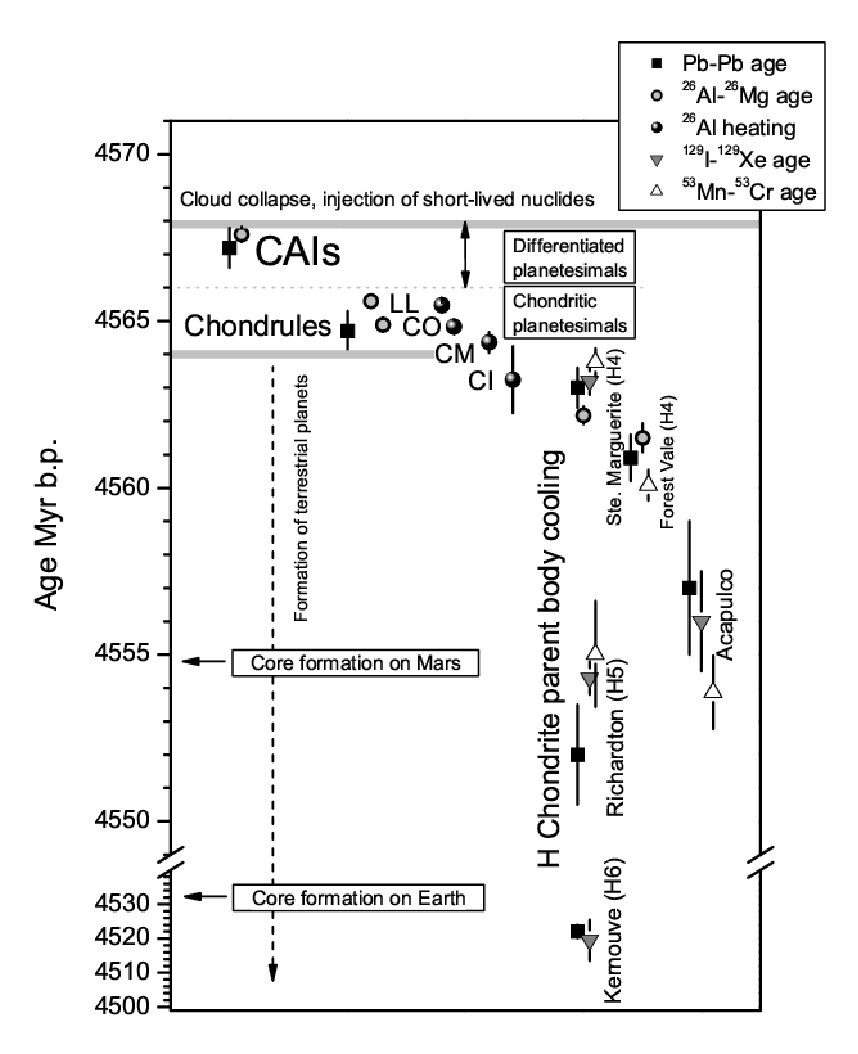
\includegraphics[width=8cm]{d1fig1.eps}}
\caption{Calibration of radioisotope time scales of early solar system
rocks: Pb-Pb (G\"opel et al.\ 1994; Amelin et al.\ 2002), Mn-Cr (Lugmair \&
Shukolyukov 1998, 2001; Polnau \& Lugmair 2001; Polnau et al.\ 2000), Al-Mg
(Zinner \& G\"opel 1992; Russell et al.\ 1996, 2001; Kita et al.\ 2000,
2004; Kunihiro et al.\ 2004), I-Xe (Nichols et al.\ 1994, Brazzle et al.\
1999). Red symbols are timescales according to planetesimal heating by
$^{26}$Al, from Trieloff and Palme (2006). }
\end{figure}

\subsection{Analysis of cometary matter returned by the STARDUST mission}

Comets have long been regarded as the chemically most primitive bodies in
our solar system, mostly due to their high abundance of volatiles: C, H, O,
N plus noble gases, at a level between solar and CI chondrite
composition. Particularly super-volatile species like CO demand that they
were stored most of their time at very low temperatures after
formation. However, IR spectroscopy of Hale-Bopp (Wooden et al.\ 2000)
already indicated that crystalline Mg-rich dust (forsterite, enstatite) is
present, an unexpected observation as these silicates are thought to be high
temperature products. Nevertheless this is in line with observations that
most of the sub-particles analyzed with NANO-SIMS in Interplanetary Dust Particles (IDPs) of presumably
cometary origin are isotopically solar (Messenger et al.\ 2003), and partly
have a high temperature origin, and also in line with one of the first
STARDUST results that CAI-like material was found among comet Wild-2
particles. As many scientists believe that these high temperature products
stem from the inner warm zones of our early solar system, these observations
have aroused strong interest in radial mixing processes of protoplanetary
discs, and in fact the observations place fundamental constraints on the
magnitude of these processes. The crucial number to be extracted from the
analysis of cometary dust is to identify and quantify the fraction of
material that experienced high temperature annealing, metamorphism,
condensation or evaporation and that was transported outwards subsequently. This
needs structural-chemical analysis, transmission electron microscopy (TEM),
and surface-sensitive Time-of-Flight Secondary Ion Mass Spectrometry
(TOF-SIMS). It is furthermore of importance to show that this material is
isotopically solar, i.e.\ equilibrated in the solar system, in order to
exclude the possibility that e.g.\ Mg-rich silicates are remnants of high
temperature condensation processes in the stellar envelope of a precursor
star nearby the cloud from which the solar nebula collapsed. This can only
be performed on sample returned material in the laboratory by NANO-SIMS
analysis. STARDUST (Brownlee et al.\ 1996) is the first extraterrestrial
sample return mission since the Apollo program, and the ongoing analysis can
provide such results, provided that systematic strategies are applied to
investigate keeping these goals in mind.


\section{Preliminary work (Eigene Vorarbeiten)}

M. Trieloff has broad experience in cosmochemistry and geochemistry,
particular the isotope radio-chronometry of processes in the early solar
system and their relationship to astrophysical processes in protoplanetary
disks. M. Trieloff conducted a number of studies on early meteorite
chronology and the accretionary and cooling history of meteorite parent
bodies (Trieloff et al.\ 2003; Kunz et al.\ 1995; Pellas et al.\ 1997;
Korochantseva et al.\ 2005). Combined $^{40}$Ar-$^{39}$Ar dating and $^{244}$Pu
fission track dating demonstrated that Acapulco and H4 chondrites Forest
Vale, St. Marguerite, and H5 Richardton are meteorites that formed early and
cooled rapidly in the high temperature (and partly also low temperature)
regime, i.e.\ that they recorded primary cooling histories and that later
secondary disturbances were insignificant.

M. Trieloff also studied processes that are related to the clearing of
accretions disk in the early solar nebula, leading to solar wind
implantation into precursor planetesimals of meteorite parent bodies and the
terrestrial planets (Trieloff et al.\ 2000, 2002; Trieloff and Kunz, 2005;
Schwarz et al.\ 2005). Trieloff and Palme (2006) reviewed and outlined the
early solar system history as seen by meteoriticists in the context of
astrophysical processes and disk evolution, specifically aimed at
astrophysically oriented scientists working on planet formation processes.

M. Trieloff has particular experience with $^{40}$Ar-$^{39}$Ar dating of
meteoritic matter (Trieloff et al.\ 2003; Kunz et al.\ 1995; Pellas et al.\
1997; Korochantseva et al.\ 2005) and implicitly the handling of neutron
irradiated samples as necessary for $^{129}$I-$^{129}$Xe
dating. $^{129}$I-$^{129}$Xe dating belongs to traditional noble gas studies
and was performed in Heidelberg previously (Jordan et al.\ 1980).

R. Altherr has broad expertise in the field of hard-rock petrology,
geochemistry and K-Ar geochronology. He has worked on the geodynamic
evolution of the Aegean, the Variscan belt of Central Europe and the Alps
including the formation of ultrahigh- and high-pressure metamorphic rocks
during subduction and continental collision (e.g.\ Altherr et al.\ 1979;
Schliestedt et al.\ 1988; Becker and Altherr, 1992; Kalt et al.\ 1995;
Altherr and Kalt, 1996; Kalt and Altherr, 1996; Paquin and Altherr,
2001). Another field of expertise are geochemical and petrographic studies
on high pressure and UHP mantle rocks (Paquin and Altherr, 2002, 2004;
Woodland et al.\ 2002; Olker et al.\ 2003; Witt-Eickschen et al.\ 2003).

The SIMS laboratory at the Mineralogical Institute has one of the few
national ion microprobes dedicated to geoscientific research. There
is experience with elemental and isotopic analysis of many elements, in
recent years focusing on Li, Be and B.

T. Stephan is member of four sub-teams of the STARDUST preliminary
examination team and correspondingly involved in the ongoing preliminary
examination phase for the STARDUST samples. There is considerable experience
in the analysis of cosmic dust (e.g.\ Stephan et al.\ 1994). In 1994,
T. Stephan initiated a still ongoing comprehensive consortium study of
particles from the stratospheric particle collector U2071 (Stephan et al.\
2001; Rost et al.\ 1998, 1999a, 1999b). In the last couple of years, IDP
research was focused on the identification of carriers of isotopic
anomalies, mainly 15N enrichments, in IDPs (Stephan and Stadermann, 2001;
Stephan, 2002; Stephan et al.\ 2003). This study in collaboration with the
Washington University in St. Louis brings together TOF-SIMS and NanoSIMS as
complementary techniques. Several IDPs from collector U2071 were
recently investigated at the Institute for Planetology in M\"unster and the
Max-Planck-Institute for Chemistry in Mainz (Hoppe et al.\ 2005; Stephan et
al.\ 2005). TEM in combination with TOF-SIMS and NanoSIMS allows a clear
structural identification of minerals that is not possible with the chemical
and isotopic information alone.  Together with established electron
microscope techniques (like SEM, TEM, and EMPA/electron microprobe analysis)
T. Stephan�s group uses especially TOF-SIMS for the analysis of small
grains. He introduced TOF-SIMS into the field of cosmochemistry and applied
this technique to the analysis of IDPs, presolar grains, and fine-grained
material in meteorites (e.g.\ Stephan 2001).



%
% Here follows the own refereed publications by the PIs in relation to
% the project proposed here.
%
\ownpubltitle{Own publications related to the Forschergruppe:}
%
% BELOW IS ONLY AN EXAMPLE OF TWO ENTRIES. SEE THE ADDITIONAL FILES 
% SENT TO YOU WITH ALL THE REFERENCES FROM THE VORANTRAG
%
\begin{ownpubl}
\item Altherr R. and Kalt A. (1996) Metamorphic evolution of ultrahigh-pressure garnet peridotites form the Variscan Vosges Mts. (France). Chem. Geol. \textbf{134}, 27-47.
\item Altherr R., Schliestedt M.,  Okrusch M., Seidel E., Kreuzer H., Harre W., Lenz H., Wendt I., Wagner G.A. (1979) Geochronology of high-pressure rocks on Sifnos (Cyclades, Greece). Contrib. Mineral.\ Petrol. \textbf{70}, 245-255.
\item Becker H. and Altherr R. (1992) Evidence from ultra-high-pressure marbles for recycling of sediments into the mantle. Nature \textbf{358}, 745-748.
\item Hoppe P., Mostefaoui S., and Stephan T. (2005) NanoSIMS oxygen- and
  sulfur-isotope imaging of primitive solar system materials. Lunar
  Planet. Sci. \textbf{36}, \# 1301 (abstr.).
\item Kalt A. and Altherr R. (1996) Metamorphic evolution of garnet-spinel peridotites from the Variscan Schwarzwald (Germany). Geol. Rundschau \textbf{85}, 211-224.
\item Kalt A., Altherr R., Hanel M. (1995) Contrasting P-T conditions recorded in ultramafic high-pressure rocks from the Variscan Schwarzwald (F.R.G.). Contrib. Mineral.\ Petrol. \textbf{121}, 45-60.
\item Korochantseva, E.V., Trieloff, M., Buikin, A.I., Meyer, H.P. and Hopp, J. (2005) Argon-40/Argon-39 dating, and cosmic ray exposure time of desert meteorites: Dhofar 300 and Dhofar 007 eucrites and anomalous achondrite NWA 011. \textit{Meteoritics and Planetary Science\/}, \textbf{40}, 1433
\item Kunz J., Trieloff M., Bobe K., Metzler K., St\"offler D., and Jessberger E.K. (1995) The collisional history of the HED parent body inferred from $^{40}$Ar-$^{39}$Ar ages of Eucrites. \textit{Planetary and Space Science\/}, \textbf{43}, 527-543.
\item Olker B, Altherr R, Paquin J (2003) Fast exhumation of the ultrahigh-pressure Alpe Arami garnet peridotite (Central Alps, Switzerland): constraints from geospeedometry and thermal modelling. Journal of Metamorphic Geology \textbf{21}, 395-402
\item Paquin J, Altherr R (2001) New constraints on the P-T evolution of the Alpe Arami garnet peritotide body (Central Alps, Switzerland). Journal of Petrology \textbf{42}, 1119-1140 
\item Paquin J, Altherr R (2002) Subduction-related lithium metasomatism during exhumation of the Alpe Arami ultrahigh-pressure garnet peridotite (Central Alps, Switzerland). Contributions to Mineralogy and Petrology \textbf{143}, 623-640 
\item Paquin J, Altherr R, Ludwig T (2004) Li-Be-B systematics in the ultrahigh-pressure garnet peridotite from Alpe Arami (Central Swiss Alps): implications for slab-to-mantle transfer. Earth and Planetary Science Letters \textbf{218}, 507-519 
\item Pellas, P., Fieni, C., Trieloff, M. and Jessberger, E.K. (1997) The cooling history of the Acapulco meteorite as recorded by the $^{244}$Pu and $^{40}$Ar-$^{39}$Ar chronometers. \textit{Geochimica et Cosmochimica Acta\/}, \textbf{61}, 3477
\item Rost D., Stephan T., and Jessberger E. K. (1999a) Surface analysis of stratospheric dust particles. Meteorit. Planet. Sci. \textbf{34}, 637�646. 
\item Rost D., Stephan T., Jessberger E. K., Nakamura K., and Kl\"ock W. (1998) New TOF-SIMS analyses of sections from stratospheric dust particles. Lunar Planet. Sci. \textbf{29}, \#1637 (abstr.).
\item Rost D., Stephan T., Wies C., and Jessberger E. K. (1999b) Analysis of sections and surfaces of inter-planetary dust particles. Meteorit. Planet. Sci. \textbf{34}, A99 (abstr.).
\item Schliestedt M., Altherr R., Matthews A. (1988) Evolution of the Cycladic crystalline complex: petrology, isotope geochemistry and geochronology. In: H. C. Helgeson (Editor), Chemical Transport in Metasomatic Processes. NATO-ASI Series, Reidel, Dordrecht, pp. 389-428.
\item Schwarz W.H., Trieloff M. and Altherr R. (2005) Subduction of solar type noble gases from extraterrestrial dust: Constraints from high-pressure low-temperature metamorphic deep sea sediments. \textit{Contributions to Mineralogy and Petrology\/}, \textbf{149}, 675-684.
\item Stephan T. (2001) TOF-SIMS in cosmochemistry. Planet. Space Sci. \textbf{49}, 859�906. 
\item Stephan T. (2002) TOF-SIMS analysis of heavy-nitrogen-carrying phases in interplanetary dust. Lunar Planet. Sci. \textbf{33}, \#1352 (abstr.). 
\item Stephan T. and Stadermann F. J. (2001) Preliminary identification of a heavy-nitrogen-carrying phase in IDPs. Meteorit. Planet. Sci. \textbf{36}, A197�A198 (abstr.). 
\item Stephan T., Arndt P., Jessberger E. K., Kl\"ock W., Nakamura K., Maetz M., Rost D., Thomas-Keprta K. L., Warren J. L., Weber I., and Wies C. (2001) Comprehensive consortium study of interplanetary dust particles from collector U2071. Lunar Planet. Sci. \textbf{32}, \#1267 (abstr.). 
\item Stephan T., Jessberger E. K., Kl\"ock W., Rulle H., and Zehnpfenning J. (1994) TOF-SIMS analysis of interplanetary dust. Earth Planet. Sci. Lett. \textbf{128}, 453�467. 
\item Stephan T., Leitner J., Floss C., and Stadermann F. J. (2003) TOF-SIMS analysis of isotopically anomalous phases in interplanetary dust and Renazzo. Lunar Planet. Sci. \textbf{34}, \#1343 (abstr.). 
\item Stephan T., Weber I., and Hoppe P. (2005) TOF-SIMS, NanoSIMS, and TEM analysis of interplanetary dust particle sections. Lunar Planet. Sci. \textbf{36}, \#1645 (abstr.).
\item Trieloff, M. and Kunz, J. (2005) Isotope systematics of noble gases in the Earth�s mantle: Possible sources of primordial isotopes and implications for mantle structure. \textit{Physics of the Earth and Planetary Interiors\/}, \textbf{148}, 13
\item Trieloff, M. and Palme, H. (2006) The origin of solids in the early solar system. In: \textit{Planet Formation - Theory, Observations, and Experiments}. (Eds. H. Klahr, W. Brandner), Cambridge University Press, Cambridge, 64
\item Trieloff, M., Falter, M., Buikin, A.I., Korochantseva, E.V., Jessberger, E.K. and Altherr R. (2005) Argon isotope fractionation induced by stepwise heating. \textit{Geochimica et Cosmochimica Acta\/}, \textbf{69}, 1253
\item Trieloff, M., Jessberger, E.K., Herrwerth, I., Hopp, J., Fi�ni, C., Gh�lis, M., Bourot-Denise, M. and Pellas, P. (2003) 244Pu and 40Ar-39Ar thermochronometries reveal structure and thermal history of the H-chondrite parent asteroid. \textit{Nature\/}, \textbf{422}, 502
\item Trieloff, M., Kunz, J. and All�gre, C.J. (2002) Noble gas systematics of the R�union mantle plume source and the origin of primordial noble gases in Earth�s mantle. \textit{Earth and Planetary Science Letters\/}, \textbf{200}, 297
\item Trieloff, M., Kunz, J., Clague, D.A., Harrison, D. and All�gre, C.J. (2000) The nature of pristine noble gases in mantle plumes. \textit{Science\/}, \textbf{288}, 1036
\item Witt-Eickschen G, Seck HA, Mezger K, Eggins SM, Altherr R (2003) Lithospheric mantle evolution beneath the Eifel (Germany): constraints from Sr-Nd-Pb isotopes and trace element abundances in spinel peridotite and pyroxenite xenoliths. Journal of Petrology \textbf{44}, 1077-1095 
\item Woodland AB, Seitz H-M, Altherr R, Marschall H, Olker B, Ludwig T (2002) Li abundances in eclogite minerals: a clue to a crustal or mantle origin? Contributions to Mineralogy and Petrology \textbf{143}, 587-601
\end{ownpubl}
%



\section{Goals (Ziele)}
\begin{enumerate}
\item Isotope chronology of chondrule populations
\begin{compactitemize}
\item Determine age constraints for planetesimal formation by applying I-Xe and
  $^{26}$Al-$^{26}$Mg chronometry to chondrules. Check age distributions of
  chondrule populations of single meteorites and differences between age
  distributions of meteorites from different classes, mainly between
  ordinary and carbonaceous chondrites.
\item Constrain models of timing of planetesimal growth in the early solar
  system, i.e.\ duration of accretion of single parent bodies, sequence of
  accretion of different parent bodies: how many Myr after CAIs did
  individual parent bodies accrete, how long did they need for accretion,
  and what was the age of the accreted precursor chondrules?
\end{compactitemize}
\item Analysis of cometary matter returned by the STARDUST mission
\begin{compactitemize}
\item Quantify the proportion of high temperature products (thermally
annealed crystalline material, high temperature condensates or evaporation
residues). Constrain fraction of the material that originated from the inner
disk and were transported into the outer disc regions where comets
formed. While TEM and TOF-SIMS analyses will allow to infer the
structural-mineralogical-chemical state of cometary dust (amorphous,
crystalline, chemical composition), NANO-SIMS studies will further quantify
the fraction of unprocessed interstellar dust and dust components processed
in the early solar system. These numbers constrain radial mixing processes
to the outer disk, and are needed in project A2.
\end{compactitemize}
\end{enumerate}



\section{Work schedule (Arbeitsprogramm)}

(this section only refers to goal Isotope chronology of chondrule
populations. STARDUST analyses are described and performed in a separate DFG
proposal, code no. STE 576/17

\subsection{Methods}
The basic strategy will be to use two different short-lived nuclide systems
($^{129}$I-$^{129}$Xe, $^{26}$Al-$^{26}$Mg) in order to check age
distributions that previously relied on one single chronometer. For this
study the Heidelberg Mineralogical institute has experienced laboratory
facilities. Different diffusion parameters of daughter nuclides in relevant
host minerals (Mg, Xe) should allow to distinguish artifacts, e.g.\ if shock
or thermally induced (partial or complete) reset of radiometric systems
causes irrelevant low ages, or if incomplete reset of the radiometric clock
during formation causes irrelevant high ages. For I-Xe dating of chondrules,
improvements could be achieved by a more comprehensive identification of
host phases carrying iodine. Such phases can be searched for in individual
chondrules using combined electron and ion microprobe studies. Iodine should
be enriched in the mesostasis, but pyroxene is a potential carrier as well
(Pravdivtseva et al.\ 1998). It may also be feasible to identify (and remove
by mineral separation or etching) iodine phases of low xenon retentivity in
order to avoid phases disturbed by secondary events.

Chondrules will be separated from selected meteorites from different
chondrite classes. Meteorites must be chosen in which the radiometric
systems are not or not recognizably disturbed by processes following
chondrule formation (thermal or aqueous metamorphism on the parent body,
impact/shock induced reheating). Ar-Ar data from an unpublished doctoral
thesis in Heidelberg (Herrwerth, 1983), and other I-Xe and
$^{26}$Al-$^{26}$Mg studies will help to select appropriate
samples. Chondrites with an obvious undisturbed I-Xe system of chondrules
are L4 Bjurb\"ole and - possibly - CV3 Allende (see compilation by Whitby,
2004). L4 Saratov and H4 Ochansk have easily separable chondrules with
undisturbed K-Ar systems (Herrwerth 1983). CO 3.0 Y81020 and the H
chondrites H3 Tieschitz, H4s Forest Vale, Ste. Marguerite, Beaver Creek,
Ankober, Quenggouk are worthwhile to be checked based on their low
processing degree established by $^{26}$Al-$^{26}$Mg, $^{40}$Ar-$^{39}$Ar
and $^{244}$Pu fission track studies (Kunihiro et al.\ 2004; Zinner \&
G\"opel. 1992; Trieloff et al.\ 2003). Some LL3 chondrites (e.g.\ 3.4
Chainpur, 3.6 Parnallee) are disturbed in their Ar-Ar and I-Xe systems
(Herrwerth 1983; Whitby 2004). Part of the chondrules from 3.0 Semarkona
seem also disturbed in the I-Xe system (Whitby 2004), while the Al-Mg system
of most chondrules from this meteorite seems to record primary formation
events (Kita et al.\ 2000, 2004). Further studies on LL3.1 Bishunpur can
supplement the study, and other promising meteorite samples will be searched
on in the course of the study.

We are - of course - aware of the problem that parent body metamorphism
(reflected in petrologic type) may have reset radiometric systems. However,
the fact that 3.4 or 3.6 LL chondrites (Chainpur, Parnallee) are disturbed,
may not imply that stronger metamorphosed type 4 chondrites were disturbed
or reset as well. In the case of Chainpur, Ar-Ar ages indicate that
disturbances happened a few 100 Ma after thermal metamorphism (Herrwerth,
1983). Hence, not parent body metamorphism itself (reflected in the subtype
3.4 classification) was the likely cause of disturbance, but probably
secondary impact metamorphism induced by a collisional event. Bjurb\"ole,
although of petrologic type 4, has whole rock ages well up to 2-4 Ma older
than Shallowater enstatite (Brazzle et al.\ 1999; Gilmour et al.\ 2006),
well within the range of earliest chondrule ages (Gilmour et al.\ 2006), so
a reset of the clock by parent body metamorphism is not evident, at least
not obvious. On the other hand, the I-Xe and Al-Mg system of H4
Ste. Marguerite feldspar (this secondary mineral phase formed upon thermal
parent body metamorphism) seems to have recorded a post chondrule formation
event, most likely (rapid) cooling due to parent body metamorphism. In this
context it is important to note that the petrologic type 4 classification (a
discrete classification scheme) encompasses a wide range of maximum
metamorphic temperatures ranging from 600�C-700�C. This is also reflected by
the varying integration degrees of chondrules and matrix, and implies the
possibility that the degree of disturbance of specific meteorites and their
mineral phases could have been very different, and does not exclude type 4
chondrites as possible sample for the studies suggested here.

From each ordinary chondrite / carbonaceous chondrite sample, 10-20
chondrules will be separated. While the larger parts of them will be kept
for possible I-Xe analysis, a smaller part will be sectioned and classified
by optical and electron microscopy. Electron microprobe analysis will
further help to classify chondrules, establish mineralogical/petrographic
properties and enable subsequent ion microprobe studies. Preliminary ion
microprobe inspections will allow the recognition of $^{26}$Mg excess, and
possible iodine carrier phases in chondrules (mesostasis, pyroxene, etc),
including their iodine concentrations, in order to select the most promising
samples for I-Xe analysis.

I-Xe analysis of single chondrules with phases enriched in iodine (of
different chondrite types) and the possible use of cumulate samples of type
I, type II chondrules will lead to an increased precision. Moreover, the use
of mineral separates (e.g.\ pyroxene) seems advisable to get a better
control of carrier phases, closure temperatures and comparability of
results/I-Xe ages. Particularly pyroxene is a more retentive carrier for
argon (as monitored by neutron induced $^{37}$Ar, e.g.\ Trieloff et al.\
2003) and hence a promising candidate for a retentive, undisturbed host
phase of radiogenic $^{129}$Xe. Separates of the Shallowater I-Xe standard
shall be used throughout the project; we will additionally check the
homogeneity of the Iodine distribution via SIMS.

For samples successfully dated with I-Xe, ion microprobe investigations can
� if not succeeded during the preliminary investigation - constrain
iodine carrier phases (especially in the light of degassing reservoirs
identified during Xe analyses), and will perform $^{26}$Al-$^{26}$Mg dating
of individual chondrules. Comparison of these data will allow to check for
age differences within chondrule populations (e.g.\ possibly dependent on
chondrule chemistry), and to quantify age distributions. The ultimate goal
is to compare the age distributions between different meteorite classes. The
most favorable case would be to obtain consistent results of the two
chronometric systems, but also inconsistent results can yield valuable
information: they could indicate that the different chronometers date
different events, or were incompletely reset or responded differently to
subsequent disturbances. Just as an example, if I-Xe does not reproduce
older chondrule ages from $^{26}$Al-$^{26}$Mg, this could mean that the
$^{26}$Al-$^{26}$Mg was not completely reset during chondrule formation,
i.e.\ that high chondrule ages are not formation ages.

Personal support and laboratory equipment in Heidelberg for mineral
separation and chondrule preparation, SEM and electron microprobe analytical
facilities, noble gas mass spectrometer for analysis of neutron irradiated
samples, ion microprobe is available. The noble gas lab in Heidelberg is one
of the few worldwide (and only one in Germany) engaged in dating with noble
gas nuclides of neutron irradiated extraterrestrial samples, and has
significant expertise in this field (e.g.\ Trieloff et al.\ 2003; Kunz et
al.\ 1995; Pellas et al.\ 1997; Korochantseva et al.\ 2005). In addition to
Ar-Ar dating, I-Xe dating can be performed with the same technique (neutron
irradiated samples, noble gas isotope analysis), but yields a better time
resolution/precision for early solar system processes. Moreover, Heidelberg
has one of the few ion microprobes used for geological/extraterrestrial
samples. The ion microprobe analytic facility has been repeatedly improved
by in-house constructional efforts. Ion microprobe analyses are the standard
technique for $^{26}$Al-$^{26}$Mg dating.


\subsection{Schedule}
\subsubsection{First year}

Preparation of chondrule separates of various ordinary and carbonaceous
chondrites (if appropriate mineral separations) and I-Xe dating
standards. Mineralogical/petrographic characterization of chondrule thin
sections (Optical, SEM, EMPA), and first SIMS analyses. Irradiation and
first xenon isotope dating.

\subsubsection{Second year}

Continuation of xenon isotope dating, EMPA analyses and Mg isotope
measurements with ion microprobe.

\subsubsection{Third year}

Final experiments/analyses, preparation of thesis and publications


\subsection{Literature}
%
% Here follows a general literature list related to the topic of the
% proposal, just like a literature list for a scientific paper.
%
% AGAIN ONLY EXAMPLES ARE LISTED NOW
%
\begin{literature}
\item All\`egre, C.J., Manh\`es, G., and G\"opel C. (1995).  The age of the Earth, \textit{Geochim. Cosmochim. Acta} \textbf{59}, 1445--1456.   
\item Amelin Y., Krot A. N., Hutcheon I.D. and Ulyanov A.A. (2002).  Lead isotopic ages of chondrules and calcium-aluminum-rich inclusions.  \textit{Science} \textbf{297}, 1678--1682.   
\item Amelin Y. (2006) The prospect of high precision Pb isotopic dating of meteorites. \textit{Met. Planet. Sci.} 41, 7-17.
\item Birck, J.-L. and All\`egre, C. J. (1985).  Evidence for the presence of $^{53}$Mn in the early Solar System, \textit{Geophys. Res. Lett.} \textbf{12}, 745--748.
\item Bizzarro, M., Baker, J. A. and Haack, H. (2004).  Mg isotope evidence for contemporaneous formation of chondrules and refractory inclusions, \textit{Nature} \textbf{431}, 275--278.
\item Bockel\'ee-Morvan, D., Gautier, D., Hersant, F., Hur\'e, J.M., and Robert, F. (2002) Turbulent radial mixing in the solar nebula as the source of crystalline silicates in comets. \textit{Astronomy and Astrophysics\/}, \textbf{384}, 1107
\item Boss A.P. and Vanhala H.A.T. (2001).  Injection of newly synthesized elements into the protosolar cloud, \textit{Phil. Trans. R. Soc. Lond.} \textbf{A 359}, 2005--2017.   
\item Brazzle R.H., Pravdivtseva O.V., Meshik A.P. and Hohenberg C.M. (1999).  Verification and interpretation of the I-Xe chronometer.  \textit{Geochim. Cosmochim Acta} \textbf{63}, 739--760.   
\item Brownlee D. E., Burnett D. {\em et~al.} (1996).  Stardust: Comet and interstellar dust sample return mission, in \textit{Physics, Chemistry, and Dynamics of Interplanetary Dust}, ed. B.A.S.~Gustafson and M.S.~Hanner (ASP Conf. Series 104).   
\item Chen J.H. and Wasserburg G.J. (1981).  The isotopic composition of uranium and lead in Allende inclusions and meteoritic phosphates.  \textit{Earth Planet. Sci. Lett.} \textbf{5}, 15--21.   
\item Desch, S. J. and Connolly Jr., H. C. (2002).  A model of the thermal processing of particles in solar nebula shocks: application to the cooling rates of chondrules.  \textit{Meteoritics and Planetary Science} \textbf{37}, 183.   
\item Dodd R. T. (1969).  Metamorphism of the ordinary chondrites: A review.  \textit{Geochim. Cosmochim. Acta} \textbf{33}, 161--203.   
\item Gail, H.-P. (2003).  Formation and evolution of minerals in accretion disks and stellar outflows, in \textit{Astromineralogy }, ed. T.K.~Henning (Springer, Heidelberg).   
\item Gail, H.-P. (2004).  Radial mixing in protoplanetary accretion disks IV. Metamorphosis of the silicate dust complex.  \textit{Astron. Astrophys.} \textbf{413}, 571--591.   
\item Gilmour J.D., Pravdivtseva O.V., Busfield A., and Hohenberg C.M. (2004).  I-Xe and the chronology of the early solar system.  \textit{Workshop on chondrites and the protoplanetary disk} abstr. no. 9054.
\item Gilmour J.D., Pravdivtseva O.V., Busfield A., and Hohenberg C.M. (2006).  The I-Xe chronometer and the early solar system.  \textit{Met. Planet. Sci.} 41, 19-31.
\item Gilmour J.D. and Saxton, J.M. (2001).  A time-scale of formation of the first solids, \textit{Phil. Trans. R. Soc. Lond.} \textbf{A 359}, 2037--2048.   
\item G\"opel C., Manh\`es G., and All\`egre C.J. (1994).  U-Pb systematics of phosphates from equilibrated ordinary chondrites.  \textit{Earth Planet. Sci. Lett.} \textbf{121}, 153--171.   
\item Halliday A.N., Lee D-C. {\em et~al.} (2001).  The rates of accretion, core formation and volatile loss in the early Solar System.  \textit{Phil. Trans. R. Soc. Lond.} \textbf{A 359}, 2095.   
\item Hartmann L. (2001).  Physical conditions of protosolar matter.  \textit{Phil. Trans. R. Soc. Lond.} \textbf{A 359}, 2049--2060.
\item Herrwerth I., M\"uller N., Jessberger E.K., Kirsten T. (1983) $^{40}$Ar-$^{39}$Ar Dating of Individual Chondrules and the Siting of Trapped Argon. Met. 18, 311.
\item Jeffery P.M. and Reynolds J.H. (1961).  Origin of excess Xe$^{129}$ in stone meteorites.  \textit{J. Geophys. Res.} \textbf{66}, 3582--3583.   
\item Jordan, J.; Kirsten, T.; Richter, H. (1980) I-129/I-127 - A puzzling early solar system chronometer. Z. Naturforschung 35 a, 145-170.
\item Kita N.T., Nagahara H., Togashi S. and Morishita Y. (2000).  A short duration of chondrule formation in the solar nebula: Evidence from Al-26 in Semarkona ferromagnesian chondrules \textit{Geochim. Cosmochim. Acta} \textbf{64}, 3913--3922.
\item Kita N.T., Huss G.R. {\em et~al.} (2004).  Constraints on the origin of chondrules and CAIs from short-lived and long-lived radionuclides.  \textit{Workshop on chondrites and the protoplanetary disk, abstr. no \#9064.}   
\item Kleine, T., M\"unker, C. {\em et~al.} (2002).  Rapid accretion and early core formation on asteroids and the terrestrial planets from Hf-W chronometry.  \textit{Nature} \textbf{418}, 952.
\item Kleine, T., Mezger, K., Palme, H., Scherer, E. and M\"unker, C. (2005).  Early core formation in asteroids and late accretion of chondrite parent bodies: Evidence from 182Hf-182W in CAIs, metal-rich chondrites and iron meteorites.  \textit{Geochim. Cosmochim. Acta}, \textbf{69}, 5805
\item Klerner S. and Palme H. (2000).  Formation of chondrules and matrix in carbonaceous chondrites.  \textit{Met. Plan. Sci.} \textbf{35}, A89.   
\item Kn\"odlseder J., Cervino M., Le Duigou J.M., Meynet G., Schaerer D. and von Ballmoos P. (2002).  Gamma-ray line emission from OB associations and young open clusters - II. The Cygnus region.  \textit{Astron. Astrophys.} \textbf{390}, 945--960.   
\item Kokubo, E. and Ida, S. (2000).  Formation of protoplanets from planetesimals in the solar nebula.  \textit{Icarus} \textbf{143}, 15. 
\item Kunihiro T., Rubin A.E., McKeegan K.D. and Wasson J.T. (2004).  Initial $^{26}$Al/$^{27}$Al in carbonaceous-chondrite chondrules: Too little $^{26}$Al to melt asteroids.  \textit{Geochim. Cosmochim. Acta} \textbf{68}, 2947--2957.    
\item Kurahashi, E.; Kita, N. T.; Nagahara, H.; Morishita, Y. (2004) Contemporaneous Formation of Chondrules in the $^{26}$Al-$^{26}$Mg System for Ordinary and CO Chondrites. Lun. Planet. Sci. XXXV, abstract no.1476
\item LaTourrette T. and Wasserburg G.J. (1998).  Mg diffusion in anorthite: implications for the formation of early solar system planetesimals.  \textit{Earth Planet. Sci. Lett.} \textbf{158}, 91--108.   
\item Lee T., Papanastassiou D.A. and Wasserburg G.J. (1976).  Demonstration of $^{26}$Mg excess in Allende and evidence for $^{26}$Al.  \textit{Geophys. Res. Lett.} \textbf{3},109--112.   
\item Lee, T., Shu, F. H. {\em et~al.} (1998).  Protostellar cosmic rays and extinct radioactivities in meteorites.  \textit{Astrophys. J.} \textbf{506}, 898.   
\item Lugmair, G.W. and Shukolyukov, A. (2001).  Early solar system events and time scales.  \textit{Met. Planet. Sci.} \textbf{36}, 1017.   
\item Lugmair G.W. and Shukolyukov A. (1998).  Early solar system timescales according to 53 Mn-53 Cr systematics.  \textit{Geochim. Cosmochim. Acta} \textbf{62}, 2863--2886.    
\item McKeegan, K. D., Chaussidon, M. and Robert, F. (2000).  Incorporation of short-lived $^{10}$Be in a calcium-aluminum-rich inclusion from the Allende meteorite.  \textit{Science} \textbf{289}, 1334--1337.   
\item Messenger, S., Keller, L. P. {\em et~al.} (2003).  Samples of stars beyond the solar system: Silicate grains in interplanetary dust.  \textit{Science} \textbf{300}, 105.   
\item Mostefaoui, S. Kita N.~T. et al. (2002)[ The relative formation ages of ferromagnesian chondrules inferred from their initial aluminum-26/aluminum-27 ratios.] Met. Planet. Sci., 37, 421.
\item Nichols, R. H., Jr.; Hohenberg, C. M.; Kehm, K, Kim Y., Marti K. (1994) I-Xe studies of the Acapulco meteorite: Absolute I-Xe ages of individual phosphate grains and the Bjurb\"ole standard. Geochim. Cosmochim Acta 58, 2553-2561.
\item Palme, H. (2001).  Chemical and isotopic heterogeneity in protosolar matter.  \textit{Phil. Trans. R. Soc. Lond.} \textbf{A 359}, 2061.   
\item Pellas P., Fieni C., Trieloff M. and Jessberger, E.K. (1997).  The cooling history of the Acapulco meteorite as recorded by the $^{244}$Pu and $^{40}$Ar-$^{39}$Ar chronometers.  \textit{Geochim. Cosmochim. Acta} \textbf{61}, 3477--3501.    
\item Polnau E. and Lugmair G.W. (2001).  Mn-Cr isotope systematics in the two ordinary chondrites Richardton (H5) and Ste. Marguerite (H4).  \textit{Lun. Planet. Sci. XXXII, abstr. no \#1527}.
\item Polnau, E.; Lugmair, G. W.; Shukolyukov, A.; MacIsaac, Ch (2000) Manganese-Chromium-Isotopic Systematics in the Ordinary Chondrite Forest Vale (H4). Meteoritics \& Planetary Science, 35, A128
\item Russell S.S., Srinivasan G., Huss G.R., Wasserburg, G.J. and MacPherson G.J. (1996).  Evidence for widespread $^{26}$Al in the solar nebula and constraints for nebula time scales.  \textit{Science} \textbf{273}, 757--762.  
\item Russell S.S., Gounelle M. and Hutchison R. (2001).  Origin of short-lived radionuclides \textit{Phil. Trans. R. Soc. Lond.} \textbf{A 359}, 1991.    
\item Scott E.R.D., Love S.G. and Krot A.N. (1996) Formation of chondrules and chondrites in the protoplanetary nebula, in \textit{Chondrules and the protoplanetary disk}, ed. R.H.~Hewins, R.H. ~Jones and E.R.D.~Scott (Cambridge University Press).   
\item Sears D.W.G. and Dodd R.T. (1988) Overview and classification of meteorites, in \textit{Meteorites and the early solar system}, ed. J.F.~Kerridge and M.S.~Matthews (University of Arizona Press, Tucson).   
\item Sears, D.W.G. (2004).  \textit{The origin of chondrules and chondrites} (Cambridge University Press).   
\item Shu F. H., Shang H. and Lee T. (1996).  Toward an astrophysical theory of chondrites.  \textit{Science} \textbf{271}, 1545--1552.    
\item Shukolyukov A. and Lugmair G. W. (1993) Life iron-60 in the early solar system.  \textit{Science} \textbf{259}, 1138--1142.   
\item Swindle and Podosek (1988). Iodine-xenon dating in: Meteorites and the early solar system, ed. Kerridge J.F. \& Matthews M.S. pp. 1127-1146. University of Arizona Press, Tucson, Arizona.
\item Tachibana S. and Huss G.R. (2003).  The initial abundance of Fe-60 in the solar system.  \textit{Astrophys. J.} \textbf{588}, L41--L44.   
\item Trieloff, M., Kunz, J. {\em et~al.} (2000).  The nature of pristine noble gases in mantle plumes.  \textit{Science} \textbf{288}, 1036--1038.   
\item Trieloff M., Kunz J. and All\`egre C.J. (2002).  Noble gas systematics of the R\'eunion mantle plume source and the origin of primordial noble gases in Earth�s mantle.  \textit{Earth Planet. Sci. Lett.} \textbf{200}, 297--313.   
\item Trieloff M., Jessberger E.K., Herrwerth I., Hopp J., Fieni C., Ghelis M., Bourot-Denise M. and Pellas P. (2003).  $^{244}$Pu and $^{40}$Ar-$^{39}$Ar thermochronometries reveal structure and thermal history of the H-chondrite parent asteroid.  \textit{Nature} \textbf{422}, 502--506.   
\item Turner G., Enright M.C. and Cadogan P. H. (1978).  The early history of chondrite parent bodies inferred from $^{40}$Ar-$^{39}$Ar ages.  \textit{Proc. Lunar Planet. Sci. Conf.} \textbf{9th}, 989--1025.    
\item van Schmus W.R. and Wood J.A. (1967).  A chemical-petrologic classification for the chondritic meteorites.  \textit{Geochim. Cosmochim. Acta} \textbf{31}, 747--765.    
\item Wasserburg, G. J., Gallino, R., and Busso, M. (1998).  \textit{Astrophys. J.} \textbf{500}, L189.    
\item Wetherill, G. W. and Stewart, G. R. (1993).  Formation of planetary embryos: Effects of fragmentation, low relative velocity, and independent variation of eccentricity and inclination.  \textit{Icarus} \textbf{106}, 190.
\item Whitby, J.A. (2004) Over What Period of Time Did Chondrule Formation Occur? \textit{Workshop on chondrites and the protoplanetary disk} abstr. no. 9101.
\item Wooden D. H., Butner, H. M. {\em et~al.} (2000).  Mg-rich silicate crystals in comet Hale-Bopp: ISM relics or solar nebula condensates?  \textit{Icarus} \textbf{43}, 126.   
\item Zinner E. and G\"opel C. (2002).  Aluminum-26 in H4 chondrites: Implications for its production and its usefulness as a fine-scale chronometer for early solar system events.  \textit{Met. Planet. Sci.} \textbf{37}, 1001--1013.   
%
%\item {\bf **************** PUT STUFF INTO ALPH ORDER ******************}
\end{literature}



\section{External/International collaborations}
\subsection{Isotope chronology of chondrule populations, Institute of Mineralogy, Heidelberg.}
\begin{collablist}
\item[Washington University, St.~Louis] O.V.~Pravdivtseva, A.P.~Meshick: leading experts in
I-Xe dating, advisory team and cooperation measurements for I-Xe dating. 
\end{collablist}

\subsection{Analyses of cometary matter returned by the STARDUST mission, Institute of Planetology, M\"unster}

Intense contacts between the Institute of Planetology (M\"unster) and other
scientists investigating Stardust samples exist, especially to Prof. D. E. Brownlee (University of Washington, Seattle), Prof. G. J. Flynn (State University of New York, Plattsburgh), 
Dr. M. E. Zolensky and Dr. F. H�rz (NASA Johnson Space Center, Houston), 
Dr. Scott Sandford (NASA Ames Research Center, Moffett Field), Dr. J. P. Bradley 
(Lawrence Livermore National Laboratory). For the investigation of presolar grains from
Meteorites and IDPs, we cooperate with Prof. E. K. Zinner and Dr. S. Amari (both
Washington University, St. Louis) as well as Priv.-Doz. P. Hoppe. Especially
with Dr. Hoppe (Mainz) and Dr. Stadermann we plan to extend the joint effort to investigate
presolar phases in IDPs and the STARDUST samples. The NanoSIMS
instruments present in Mainz and St. Louis will be of great importance in this
context. In analytics, close cooperation exists
with Prof. H. Arlinghaus (Physikalisches Institut, M\"unster) as well as
Dr. E. P. Vicenzi and Dr. D. Rost (Smithsonian Institute, Washington) on
TOF-SIMS and Prof. A. Putnis (Institut f\"ur Mineralogie, M\"unster) on TEM.



\section{Link to other projects of the Forschergruppe}
  
%\begin{linkproj}
%\item[\projdul{},\projklahr{},\projtscharn{}] Data will improve the timing
%of the process of planetesimal accretion in the early solar system, and
%accordingly provides constraints on models of planetesimal growth in
%projects \projdul{}, \projklahr{}, and \projtscharn{}.
%\item[\projwolf{}] As timing of accretion/coagulation also significantly
%influences the distribution of primary dust, the project will provide
%constraints for future observations of protoplanetary disks aimed in project
%\projwolf{}. {\bf SUGGESTION BY KEES TO MARIO: Perhaps also relate to the
%measured ages of the stars, even though this is sometimes a bit
%uncertain}. Similarly, the presence of planetesimals with minerals produced
%by hydrothermal alteration processes will indicate planetesimals via the
%presence of secondary, impact induced debris dust consisting of hydrous
%silicates.
%\end{linkproj}

\begin{linkproj}
\item[C1,C2,A2] The new Isotope chronology data will improve and refine the timing of the
process of planetesimal accretion in the early solar system, and accordingly
provides constraints on models of planetesimal growth in accretion disk
models by C. Dullemond/T. Henning (C2), H. Klahr/W. Kley (C1), and
W.M. Tscharnuter/H.-P. Gail/ T. Henning (A2). 

\item[D2] As timing of accretion/coagulation also significantly influences the
distribution of primary dust, the project will provide constraints for
future observations of protoplanetary disks aimed in the project by S. Wolf
(D2). For example, the presence of planetesimals with minerals produced by
hydrothermal alteration processes will indicate planetesimals via the
presence of secondary, impact induced debris dust consisting of hydrous
silicates.

\item[A1,A2] Data obtained by STARDUST analyses will provide important constraints for
project A2 (occurrence of annealed silicates or refractory condensates in
comet formation regions). Formation conditions of such high temperature
products can be checked by experimental work to be done in A1. 

\item[B1,B2,B3] Primary
accretional textures found in cometary dust can provide important hints of
coagulation processes studied by B1, B2, B3. The chemistry and texture of
chondrites as well gives a snapshot of syn-accretional conditions. This
snapshot can be compared with the outcome of collisional experiments in
Block B, e.g. if highly porous aggregates were direct precursors before
chondrite compaction, and if chondrules or their formation processes played
a role in speeding up the planetesimal formation process.

\end{linkproj}



\section{Team members (Zusammensetzung der Arbeitsgruppe)}
%
% NOTE: Only list non-DFG-funded team members.
% NOTE: Also list technical assistants, students etc involved in the project
%
\subsection{`Isotope chronology of chondrule populations�, Institute of
  Mineralogy, Heidelberg}
\begin{teamlist}
\item[Trieloff, M., Dr. Priv. Doz.]\mbox{}\\
Team leader of noble gas isotope geochronology group.  Supervision of PhD
student, particular I-Xe measurements, integration of results and early
solar system chronology, transfer to projects A2, B1, B2, B3, C2, D2.
\item[Prof. Dr. R. Altherr, head of Mineralogical Institute]\mbox{}\\
Supervision of electron and ion microprobe measurements.
\item[Dr. H.P.-Meyer]\mbox{}\\
Electron microprobe laboratory, Mineralogical Institute: Assistance in
electron microprobe analyses.
\item[Dipl. Phys. Th. Ludwig]\mbox{}\\
Secondary Ion microprobe laboratory, Mineralogical Institute: Assistance in
ion microprobe analyses.
\item[Dr. W. Schwarz (DFG)]\mbox{}\\
Noble gas mass spectrometry laboratory, Mineralogical Institute: Assistance
in I-Xe dating experiments, noble gas mass spectrometry
\item[Dr. J. Hopp (DFG)]\mbox{}\\
Noble gas mass spectrometry laboratory, Mineralogical Institute: Assistance
in I-Xe dating experiments, noble gas mass spectrometry
\end{teamlist}
%\vspace{1em}

\subsection{`Analyses of cometary matter returned by the STARDUST mission�, 
   Institute of Planetology, M\"unster}
\begin{teamlist}
\item[HDoz. Dr. T. Stephan]\mbox{}\\
(applicant of DFG project code no. STE 576/17)
\item[Prof. Dr. E. K. Jessberger]\mbox{}\\
(applicant of DFG project code no. STE 576/17)
\item[Dipl. Phys. Jan Leitner]\mbox{}\\
(PhD student within DFG project code no. STE 576/17)
\item[N.N.]\mbox{}\\
(TEM specialist within  DFG project code no. STE 576/17)
\item[CTA Kerstin Klemm]\mbox{}\\
\end{teamlist}



\section{Funding requested}
The following table gives the full overview of requested
funding:\vspace{1\baselineskip}\\

(this section refers to `Isotope chronology of chondrule populations� only, 
the STARDUST project is funded by a separate ongoing DFG project, 
proposal code no. STE 576/17 � except for 4 travels Heidelberg-M�nster 
are applied here for collaboration STARDUST-Forschergruppe)

%
% The table that follows is the overview over the full requested 
% funding, including the positions, travel, consumables and ``other
% costs'' (which might include transportation costs of radioactive
% material or the rent of a drop tower or such).
%
\centerline{\begin{tabular}{||l|l|l|l||} \hline \hline & Year 1 & Year 2 &
Year 3 \\ \hline %
Personel (1 PhD-student: E13/2)   & \hfil 24.000 & 24.000 & 24.000 \\
Personnel (1 student research assistant (30 hours/month) & \hfil 4.500 & \hfil 2.250 & \hfil - \\
Consumables                        & \hfil 8.300 & \hfil 8.300 & \hfil 4.800 \\
Travel                             & \hfil 6.129 & \hfil 6.129 & \hfil 1.356 \\
Other costs                        & \hfil 3.200 & \hfil 3.200 & \hfil -\\
\hline
{\bf Total:}                       & \hfil 46.129 & \hfil 43.879 & \hfil 30.156 \\
\hline
\hline
\end{tabular}
}
\mbox{}\vspace{1em}\\
Below these costs are explained in more detail:

\subsection{Personnel (Personalbedarf)}
\begin{teamlist}
\item[PhD-Student 1 (E13/2)]\mbox{}\\
The doctoral student will carry out chondrule separations/preparations,
electron microprobe and ion microprobe measurements, I-Xe measurements
(noble gas mass spectrometry).
\item[Student assistant (30 h/month in first 1.5 years)]\mbox{}\\ 
A student assistant is needed to carry out time consumptive mineral
separations (e.g. pyroxene from individual chondrules).
\end{teamlist}

\subsection{Consumables (Verbrauchsmaterial)}
\subsubsection{Heidelberg}
\begin{enumerate}
\item \textbf{Noble gas mass spectrometry}\\
\begin{expenseslistnarrow}
High purity Al-foil for sample wrapping
  & \EUR &\hfill 1 700\\
Tantalum crucibles and thermocouples for resistance heated furnace
  & \EUR &\hfill 3 500 \\
Glass furnaces (kovar or duran), incl. W/Re thermocouple and Mo crucible
  & \EUR &\hfill 2 800 \\
(Crucibles and glass furnaces can be used only one time for about
4 gram neutron activated sample material. Needs external production)
  & & \\
Glass ware, chemical agents for sample purification 
  & \EUR &\hfill 600 \\
Working gases (oxygen, argon, methane)
  & \EUR &\hfill 900 \\
Consumable materials  (mass spectrometer filament, pump maintenance)
  & \EUR &\hfill 300 \\
Thermocouples to monitor getter heating
  & \EUR &\hfill 400 \\
Copper / gold wires & \EUR &\hfill 900 \\
\textbf{Total} & \EURBF & \hfill \textbf{11 100}
\end{expenseslistnarrow}
\item \textbf{Consumables for SEM, EMP, SIMS}\\
\begin{expenseslistnarrow}
Filaments, pumping oil, graphite for coating, gas, paper for videoprinter, 
spectrometer windows
  & \EUR &\hfill 4 500 \\
Preparation of polished sections: diamond paste, saw blade 
  & \EUR &\hfill   500 \\
\textbf{Total}	& \EURBF &\hfill \textbf{5 000}
\end{expenseslistnarrow}
\begin{expenseslistnarrow}
\hline
\textbf{Consumables 1st + 2nd year are equally distributed, in 3rd year
lower because experimental work mostly completed:} & & \\
\textbf{Total consumables 1st + 2nd year:} & \EURBF  &  \hfill \textbf{16 600}\\
\textbf{Consumables (Verbrauchsmaterial) (3rd year)}
  & \EURBF & \hfill \textbf{4 800}\\
\hline
\end{expenseslistnarrow}
\end{enumerate}




%Estimated cost per year:\vspace{1\baselineskip}\\
%\centerline{\begin{tabular}{|p{16em}|p{9em}|p{7em}|}
%\hline
%?        & \hfil ? & \hfil ? \\
%\hline
%\end{tabular}}


\subsection{Travel expenses in addition to Project Z (Reisekosten)}
%
% Here only travel expenses not related to usual regular Forschergruppe
% meetings and the overall per capita budget for conferences.
%
\begin{expenseslist}
PhD student will visit Washington University 2 times for about 
8 weeks (Dr. O. Pravdivtseva) to conduct I-Xe analyses. These I-Xe analyses are planned for extremely difficult analyses which require extraordinary system conditions (mass spectrometer sensitivity, low blank, etc.) St. Louis is one of the 2 laboratories worldwide where I-Xe measurements can be performed. All other measurements are planned at Heidelberg.
(56 days x (41�/day+113�/night)+2x800� flight)
  & \EUR & \hfill 10 224 \\
3 x1 week travel M\"unster (Institute of Planetology) -- Heidelberg
(Dr. Trieloff/Dr. Stephan) in the first two years for collaboration with
respect to STARDUST (21 days x (24�/day+50�/night)+3x160� train)
  & \EUR & \hfill 2 034 \\
\textbf{Total 1st + 2nd year} & \EURBF &\hfill \textbf{12 258} \\
2 x1 week travel M\"unster (Institute of Planetology) -- Heidelberg 
(Dr. Trieloff/Dr. Stephan) in the 3rd year for collaboration with respect 
to STARDUST (14 days x (24�/day+50�/night)+2x160� train)
  & \EUR & \hfill 1 356 \\
\textbf{Total 3rd year} & \EURBF &\hfill  \textbf{1 356}
\end{expenseslist}

\subsection{Investments}

None

\subsection{Other costs (Sonstige Kosten)}
\begin{expenseslist}
Costs for transport of neutron irradiated samples from GKSS (Geesthacht)	8x 800�
 Total 1st + 2nd year & \EUR &\hfill 6 400
\end{expenseslist}





\section{Preconditions for carrying out the project at home institution}
%
% This is one of the main subsections of a DFG Normalverfaren proposal.
% Several of the subsubsections in this subsection we have placed in their
% own subsections above (like team members, collaborations). What remains
% are the following three subsections. For those not familiar with these,
% we refer to the DFG Merkblatt on Normalverfahren-proposals.
%
\subsection{Scientific equipment available (Apparative Ausstattung)}
%
% Please list those larger instrument available to you for the project (if
% applicable also larger computer equipment in case you need substantial
% amounts of computer time).
%
\subsubsection{Mineralogical Institute, Heidelberg:}\mbox{}\\
\begin{compactitemize}
\item Noble gas laboratory: Various noble gas mass spectrometers routinely used for Ar-Ar dating and mantle noble gas analyses, including ultra high vacuum furnace types: induction heated glass furnaces, resistance heated double vacuum furnaces with Ta-crucibles for sample heating 
\item SEM (Leo 440) with energy dispersive system 
\item Electron microprobe CAMECA SX51
\item Laboratory for mineral separation (milling, magnetic and heavy liquid separation), optical microscopes, binocular
\item Experienced mechanical and electronics workshop  
\item Ion microprobe CAMECA 3 mf for trace element analysis, lateral resolution 10-30?m 
\item X-ray fluorescence spectrometer SIEMENS 303
\item X-ray diffractometers (Phillips, Siemens D500) 
\end{compactitemize}
\subsubsection{Institute of Planetology,  M\"unster}\mbox{}\\
Within the scope of the Interdisciplinary Center for Electron Microscopy and
Micro-analysis (ICEM), a multitude of modern analytical instruments are used
for the STARDUST proposal (DFG code no. STE 576/17
\begin{compactitemize}
\item ION-TOF TOF-SIMS IV 
\item JEM 3010 (300kV) transmission electron microscope with EDS, EELS as well as with ion mill und ultra-microtome 
\item JSM 6300F field-emission scanning electron microscope with EDS and cathodolu-minescence 
\item JEM 8600 Superprobe electron microprobe 
\item JSM 840 scanning electron microscope with EDS and Centaurus back-scatter-detector 
\item Clean room for sample preparation 
\item Light-optical microscopes
\end{compactitemize}


\subsection{Institution's general contribution (Laufende Mittel f\"ur Sachausgaben)}
%
% Please state the annual fund for consumables which comes from the
% institution's budget or any other third party  (please list separately) to
% pay for the research for which your project is part of.  Use estimates where
% applicable. 
%

Mineralogical Institute: estimated 2 000 EUR per year 






\cleardoublepage

\setcounter{equation}{0}
\setcounter{figure}{0}
%----------------------------------------------------------------------
%                        PROJECT DEFINITION
%----------------------------------------------------------------------
\renewcommand{\projnr}{D2}
\renewcommand{\projtitleshort}{Prediction of observable quantities}
\renewcommand{\projauth}{Wolf, Dullemond}
%
\setcounter{section}{0}
\noindent{\normalfont\sffamily\Large\bfseries Project \projnr: \projtitleshort}
%
\section{Full title:}
\hspace{1\baselineskip}\\
\centerline{\large ``Prediction of observable quantities}
\centerline{\large  tracing the process of planetesimal formation''}
%
\section{General information}\mbox{}
\vspace*{-1mm}
\subsection{Principle investigators:}
\hspace{-\baselineskip}\\\noindent
%
{\bfseries\itshape Wolf}, Sebastian, Dr.~\\
Leader of Emmy Noether Research Group, non-tenure\\
Date of birth: 1 June 1973, Nationality: German\\
DFG Code number of latest application: WO 857/2-2\\
Max Planck Institute for Astronomy\\
K\"onigstuhl 17\\
69117 Heidelberg\\
Tel: 06221 528 406\\
Fax: 06221 528 246\\
Email: swolf@mpia.de\\
Private address: Bogenstra\ss e 9, 69124 Heidelberg; Tel: +49-(0)6221-7360733\\
%
\vspace{1em}\\\noindent
{\bfseries\itshape Dullemond}, Cornelis P., Dr.\\
Research associate, non-tenure\\
Date of Birth: 11 December 1970, Nationality: Dutch\\
DFG Code number of latest application: N.A.\\
Max Planck Institute for Astronomy\\
K\"onigstuhl 17\\
69117 Heidelberg\\
Tel: 06221 528 395\\
Fax: 06221 528 246\\
Email: dullemon@mpia.de\\
Private address: Adolf-Rausch-Str.~4, 69124 Heidelberg; Tel: +49-(0)6221-7290263\\


\subsection{Co-investigators within this Forschergruppe:}
\begin{coilist}
\item Th.~Henning    (MPIA Heidelberg)
\item K.~Kornet      (DFG Emmy Noether group at the MPIA Heidelberg)
\item A.~Schegerer   (DFG Emmy Noether group at the MPIA Heidelberg)
\item D.~Semenov     (MPIA Heidelberg)
\item M.~Trieloff    (University Heidelberg)
\item J.~Bouwman     (MPIA Heidelberg)
\item R.~van~Boekel  (MPIA Heidelberg)
\end{coilist}

\newpage
\section{Summary (Zusammenfassung)}
\subsubsection{Summary:} 
This project aims at connecting the theoretical predictions for planetesimal
formation and evolution processes derived in the various projects of the Forschergruppe with
specific existing observations. Moreover, predictions for future observations will be investigated
providing powerful tools to verify the results of the Forschergruppe.
This project is split into two phases:
In the first part of the project, existing analytical and numerical models of protoplanetary
disks will be used to study the influence of the disk evolution on observable quantities.
As the project proceeds, at latest in the second half of it, the new results to be provided
by the other teams of the Forschergruppe will be considered. In particular, this concerns
new findings and constraints  for the evolution of the disk and the dust/planetesimals therein.
Based on the results of the radiative transfer simulations and the comparison 
with existing observations, feedback to the these teams (primarily A1/A2/B2/C1/C2/D1) 
will be provided instantaneously.
This will allow to optimize the strategy of their investigations, by providing
information about the feasibility to verify their predictions. 


\subsubsection{Zusammenfassung:} 
Ziel ist es, die in den einzelnen Projekten der Forschergruppe zu erarbeitenden 
theoretischen Vorhersagen bzgl.\ der Entstehung und Entwicklung von Planetesimalen 
relevanten, bereits vorliegenden Beobachtungsdaten gegen\"uber zu stellen. 
Dar\"uber hinaus werden Strategien f\"ur zuk\"unftige Beobachtungsprogramme erarbeitet,
um die Ergebnisse der Forschergruppe m\"oglichst umfassend verifizierbar zu machen.
Das Projekt gliedert sich in zwei Phasen:
Im ersten Abschnitt wird unter Zuhilfenahme vorliegender analytischer und numerischer
Modelle protoplanetarer Scheiben untersucht, inwiefern sich die Staub/Planetesimalentwicklung
anhand ausgew\"ahlter Beobachtungsgr\"o\ss en beschreiben l\"a\ss t.
Im zweiten Abschnitt sollen die Ergebnisse der anderen Arbeitsgruppen
bzgl.\ der Scheiben-, Staub- und Planetesimalentwicklung in die Modellierung einflie\ss en
(prim\"ar aus den Projekten A1/A2/B2/C1/C2/D1). 
Basierend auf Strahlungstransportrechnungen und dem Vergleich mit existierenden
Beobachtungen soll dann unter anderem untersucht werden, ob die experimentellen
und theoretischen Vorhersagen tat\-s\"ach\-lich mittels Beobachtungen \"uberpr\"ufbar sind.
Das Ergebnis dieser Untersuchung dient gleich\-zeitig der weiteren Planung dieser Projekte.


\section{State of the art (Stand der Forschung)}
Planets are expected to form in circumstellar disks, which are considered as
the natural outcome of the protostellar evolution, at least in the case of
low and intermediate mass stars (e.g., Adams et al.~1987;
Lissauer~1993). While a reasonably detailed picture of the structure and
evolution of circumstellar disks has been developed already, the planet
formation process is in major parts still under discussion. 
In particular, adequate constraints from observations are required in order to either
verify or rule out currently discussed planet formation scenarios (e.g.,
Pollack et al. 1996, Weidenschilling 1997, Goldreich \& Ward~1973, Youdin \&
Shu~2002).

A number of new instruments and ground and space-based observatories, which
are optimized for the observation of planet-forming/harboring disks, is now
in operation, such as the Spitzer Space Telescope operating in the mid- to far-infrared
wavelength range, long-baseline infrared
interferometers such as MIDI (Mid-Infrared Interferometric Instrument) and
AMBER (Astronomical Multiple Beam Recombiner), cameras such as NACO (Nasmyth
Adaptive Optics System + Near-Infrared Imager and Spectrograph) and VISIR
(VLT Imager and Spectrometer in the Infrared), and sub-millimeter
observatories, such as APEX (Atacama Pathfinder Experiment) and the SMA 
(Submillimeter Array).  In the near
future even more powerful observatories will provide excellent means to
study the process of planetesimal/planet formation (for example the Large
Binocular Telescope [LBT], the Stratospheric Observatory for Far-Infrared
Astronomy [SOFIA], and the Atacama Large Millimeter Array [ALMA]).  The
combination of these instruments / observatories allows /will allow to
investigate both the global structure of protoplanetary disks as well as the
planetesimal / planet-formating region and to trace various physical
processes through multi-wavelength observations.  The planned project
is in the fortunate situation to profit from the expertise in the field of
observations of circumstellar disks and instrument development at the MPIA,
where the requested PhD position will be established.  Examples for the
development and use of instruments which are particularly useful in this
context are MIDI, MATISSE (Multi Aperture Mid-Infrared Spectroscopic Experiment), NACO, and
LINC/NIRVANA (near-infrared / visible interferometric camera for the LBT).
%However, we want to
%emphasize that observations are not part of this project. Instead, our goal
%is a symbiosis between the Forschergruppe and the host institute (MPIA).

\subsection{Analyzing disks with radiative transfer tools}
In the following we summarize previous approaches to constrain the earliest
stages of planet formation through adequate observations and the
corresponding analysis via numerical modeling.  A key role is played by the
analysis of the radiation scattered and re-emitted by the dust component in
protoplanetary disks which allows to derive their opacity structure, and
thus to constrain both the dust density distribution and optical properties
of the dust grains. Besides the chemical composition and internal 
structure of the dust grains (crystalline/amorphous), their optical
properties are determined by their geometrical shape, macroscopic structure
(e.g., porous/compact, spherical/non-spherical) and size parameter
($\propto$ grain size / wavelength). Therefore, the interpretation of the
observed optical properties of the dust -- generally with the use of radiative
transfer simulations -- in principle allows to derive conclusions about grain sizes
and thus about the coagulation process.
% (see Watson et al.~2006 for a review).

Of particular interest in this respect are e.g.\ the spectroscopic features
in the infrared. The study of the shape of the 10 $\mu$m silicate feature,
for instance, allows a determination of the size of the grains as well as
their chemical composition (van Boekel et al.~2005, Schegerer et al.~2006). 
Another example is that the characteristic decrease of the polarization degree of the scattered
near-infrared radiation with increasing grain size can be used to constrain
grain sizes in optically thin regions (Fischer et al.~1996). And as a
final example: the slope of the (sub-) millimeter spectrum can
%, if the disk is shown to be optically thin at that wavelength, 
be used to constrain the grain size in the 0.1\,mm to few centimeter size regime 
(Testi et al.~2003; Rodmann et al.~2004).

Due to the high complexity of the radiation transport process even in a
simply structured disk model with rotation symmetry, only numerical
simulations provide the necessary basis for the interpretation of observed
spectral energy distributions (SEDs), intensity and polarization maps.  In
order to take into account the viewing angle effect, the minimum requirement
for simulating circumstellar disks are two-dimensional axially symmetric
models, which have been developed since the late '80s. % (e.g., Dent~1988).
However, since then the numerical description of physical processes
considered and the applied algorithms have been improved significantly (see,
e.g., Henning~2001 for a review).

Given the small number of spatially well-resolved circumstellar disks, a
proper interpretation of their SEDs is of decisive importance for studying
the disk evolution.  Unfortunately, there are many adjustable parameters in
the disk models, and several different parameter combinations usually
produce acceptable fits to the same SEDs (Thamm et al.~1994).  In particular
the flux density of disks has been observed to fall more slowly at
wavelengths longer than $\sim$400$\mu$m than those of interstellar clouds,
indicating that the emissivity exponent may be decreased due to particle
growth to $>$\,0.1\,mm (e.g., Testi et al.\,2003, Beckwith \&
Sargent~1991). However, this approach is justified only if the disk is
optically thin in this wavelength range, which can be tested through
appropriate modeling only.  Furthermore, it is usually necessary to use
additional constraints like disk inclination and geometry, such as done by
Wood et al.~(2002) who concluded from models for the SED of the classical T
Tauri star HH~30 IRS that dust grains have grown to larger than 50$\mu$m
within its circumstellar disk.

D'Alessio et al.~(2001) presented detailed models of irradiated T Tauri
disks including dust grain growth with power-law size distributions. These
models assume complete mixing between dust and gas and solve for the
vertical disk structure self-consistently including the heating effects of
stellar irradiation as well as local viscous heating. For a given total dust
mass, grain growth is found to decrease the vertical height of the surface
where the optical depth to the stellar radiation becomes unity, while
increasing the disk emission at (sub)millimeter wavelengths (see also
Dullemond \& Dominik~\cit{2004a}).  Furthermore, Dullemond \&
Dominik~(\cit{2004b}) made predictions about the influence of dust settling
on the SED and optical appearance of protoplanetary disks.

In the last few years many circumstellar disks have been studied in detail using
multi-dimensional radiative transfer tools, often with the objective to
derive their dust properties. For instance, the SED of HL Tau was studied in
this way by Men'shchikov et al.~(1999), who conclude that very
large particles causing gray extinction are abundant in the dense torus of
this object, while wavelength-dependent extinction points to submicron-sized
grains in the circumstellar envelope, which is in rough agreement with the
measured polarization degrees. Wolf et al.~(2003) studied both SED and
images of the Butterfly star with a detailed radiative transfer model. 
They showed that both SEDs and images at infrared and millimeter wavelengths
must be considered in combination in order draw robust conclusions about the
grain sizes and to eliminate degeneracies. They also find small grains in
the envelope and significantly larger grains in the disk (see Sect.~\ref{butter.model}). 
A detailed review about the importance of multi-dimensional radiative transfer modeling 
of multi-wavelengths observations for the investigation of grain size distributions
in protoplanetary disks can be found in Watson et al.~(2006).

%  As an example,
% we refer to the model of the circumstellar environment of the Butterfly star
% in Taurus by Wolf et al.~(2003) which is based on high-resolution continuum
% observations at near-infrared and millimeter wavelengths.  On the one hand,
% the millimeter-observations are sensitive to the long-wavelength radiation
% being re-emitted from the dust in the central parts close to the midplane of
% the circumstellar disk.  Furthermore, resolved millimeter images allowed to
% discriminate between different disk models with a similar
% far-infrared/millimeter SED and therefore to disentangle the disk geometry
% much more precisely.  On the other hand, the near-infrared observations
% trace the envelope structure and dust properties in the envelope and the
% disk surface.  The authors find that the grains in the envelope cannot be
% distinguished from those of the interstellar medium, while coagulation has
% already resulted in grain sizes up to $\sim$100$\mu$m in the circumstellar
% disk.

\subsection{A selection of recent observational discoveries relevant to the project}

Given the many relevant observational discoveries made in recent years related to grain growth
and evolution in disks, a comprehensive overview is not possible at this point.
Instead, we select here a few of these that might be of particular interest for this project:
\begin{itemize}
\item Recent centimeter-wavelength observations of TW Hydra indicate that
  the large grain population ($\sim$ 2.5 cm) is dominated by a narrow size
  distribution peak (Wilner et al.~2005). It is, as yet, unclear what
  this narrow size distribution is caused by.
\item Recent infrared observations with the Spitzer Space Telescope have
  revealed the existence of `transitional' objects in which the inner ($<$\,1AU)
  parts of the disk appears to be strongly depleted of dust
  (e.g.~Sicilia-Aguilar et al.~\cit{2006}). It has been suggested
  (but as yet unproven) that some of these inner holes can be explained by
  dust grain growth (e.g.~Calvet et al.~\cit{2002}; Tanaka et
  al.~\cit{2005}).
% \item In recent years the shapes of solid-state features in infrared
%   spectra of disks (e.g.~the 10 $\mu$m Si-O resonance feature and the
%   various 11-35 $\mu$m crystalline forsterite features) have been
%   interpreted in terms of the abundance of crystalline silicates and
%   the size of these grains. What do these pieces of information
%   tell about the details of coagulation and thermal processing?
\item There exist disks which have no 10\,$\mu$m silicate feature, but have
  strong features of Polycyclic Aromatic Hydrocarbons (PAHs) (Meeus et
  al.~2001).  Moreover, a number of these disks have strong
  far-infrared excesses indicative of flaring disks. It appears therefore
  that in these disks the silicate grains have grown to sizes well beyond
  10 $\mu$m, while small carbonaceous grains still exist in the disk to
  keep the disk flaring and to produce the PAH features. This poses a
  mystery for models of grain growth.
\item One would intuitively expect that the measured grain sizes increase with stellar age.
  In contrast to this, no such trend has been confirmed through the analysis of 
  the 10\,$\mu$m silicate feature (van Boekel et al.~2005).  Since
  grain growth beyond sizes of 1\,$\mu$m is anyway thought to be on time
  scales much shorter than the disk life time (e.g.~Dullemond \& Dominik
  \cit{2005}), the population of small grains is presumably regulated by
  a more complex mechanism than simple linear growth. 
\end{itemize}




\section{Preliminary work (Eigene Vorarbeiten)}\label{prelim}

% The preparatory work for the proposed project covers both observational
% studies of protoplanetary disks as well as the 
% % development and 
% application
% of numerical tools for the simulation of the continuum radiative transfer in
% dusty media, the calculation of optical properties of dust grains, and a
% parameterized approach for the formation of planetesimals / planets.  In the
% following we give an overview about selected preparatory studies:\\

%\noindent
%{\bf [a] Development of numerical tools}
%\vspace*{2mm}


\subsection{Continuum radiative transfer simulation software}\label{mc3d}
%%
Over the last decade both PIs have developed various software packages for
multi-dimensional continuum radiative transfer calculations (e.g.~Wolf et
al.~\cit{1999}, \cit{2000}; Dullemond et al.~\cit{2000}, \cit{2004a}). In
this project we will use the code {\tt MC3D} of Wolf because of its
flexibility and versatility. It allows to simulate wavelength-dependent
intensity maps and SEDs of dust configurations with discrete radiation
sources (such as one or multiple stars) as well as spatially extended, continuous heat sources
(such as accretion heating).  The density structure of the dust
configuration (for this project a protoplanetary disk), the optical
properties of the dust and the number, spatial distribution and extent, and
radiation parameters (SED, isotropy/anisotropy) of the discrete radiation
sources (stars) can be chosen arbitrarily.  The {\tt MC3D} code combines the
most recent Monte Carlo radiative transfer concepts for both self-consistent
radiative transfer, i.e., the estimation of spatial dust temperature
distributions, and pure scattering applications, taking into account the
polarization state of the radiation field. It has been tested intensively
and compared with grid-based and Monte Carlo radiative transfer codes (e.g.,
Pascucci et al.~\cit{2004}).  In order to overcome the previous limitation
to a rather small range of optical depths ($\tau < 10^3$), several
additional algorithms have been included (such as those by Cashwell \&
Everett~1959, Lucy~\cit{1999}, and Bjorkman \& Wood~\cit{2001}). We
have also developed numerical algorithms for the {\tt MC3D} which allow to
consider multiple light scattering in dust configurations containing aligned
/ non-aligned non-spherical dust grains (Wolf et al.~2002b).  Numerical methods
concerning the improved performance and tests of the {\tt MC3D} have been
published in several publications (e.g., Wolf et al.~\cit{1999}; Wolf \&
Henning~\cit{2000}; Wolf et al.~\cit{2003}).  Previous selected applications
of the {\tt MC3D} in the field of star- and planet formation cover for
example the radiative transfer in the clumpy circumstellar environment of
young stellar objects (Wolf et al.~\cit{1998}), polarization studies of
T~Tauri stars (Wolf et al.~\cit{2001}), and feasibility studies for detecting
giant extrasolar planets in circumstellar disks (Wolf et al.~\cit{2003},
Wolf \& D'Angelo~2005; see Fig.~\ref{fig-giantplanet-alma}).
%
%Beside few exceptions (see [a-2]), the {\tt MC3D} will be the general tool
%to derive observational quantities of circumstellar disks at all considered
%stages of their evolution.\\


\begin{figure}%[t!]
  \begin{center}
%    \resizebox{0.45\hsize}{!}{\includegraphics{alma_50pc.eps}}
    \resizebox{0.45\hsize}{!}{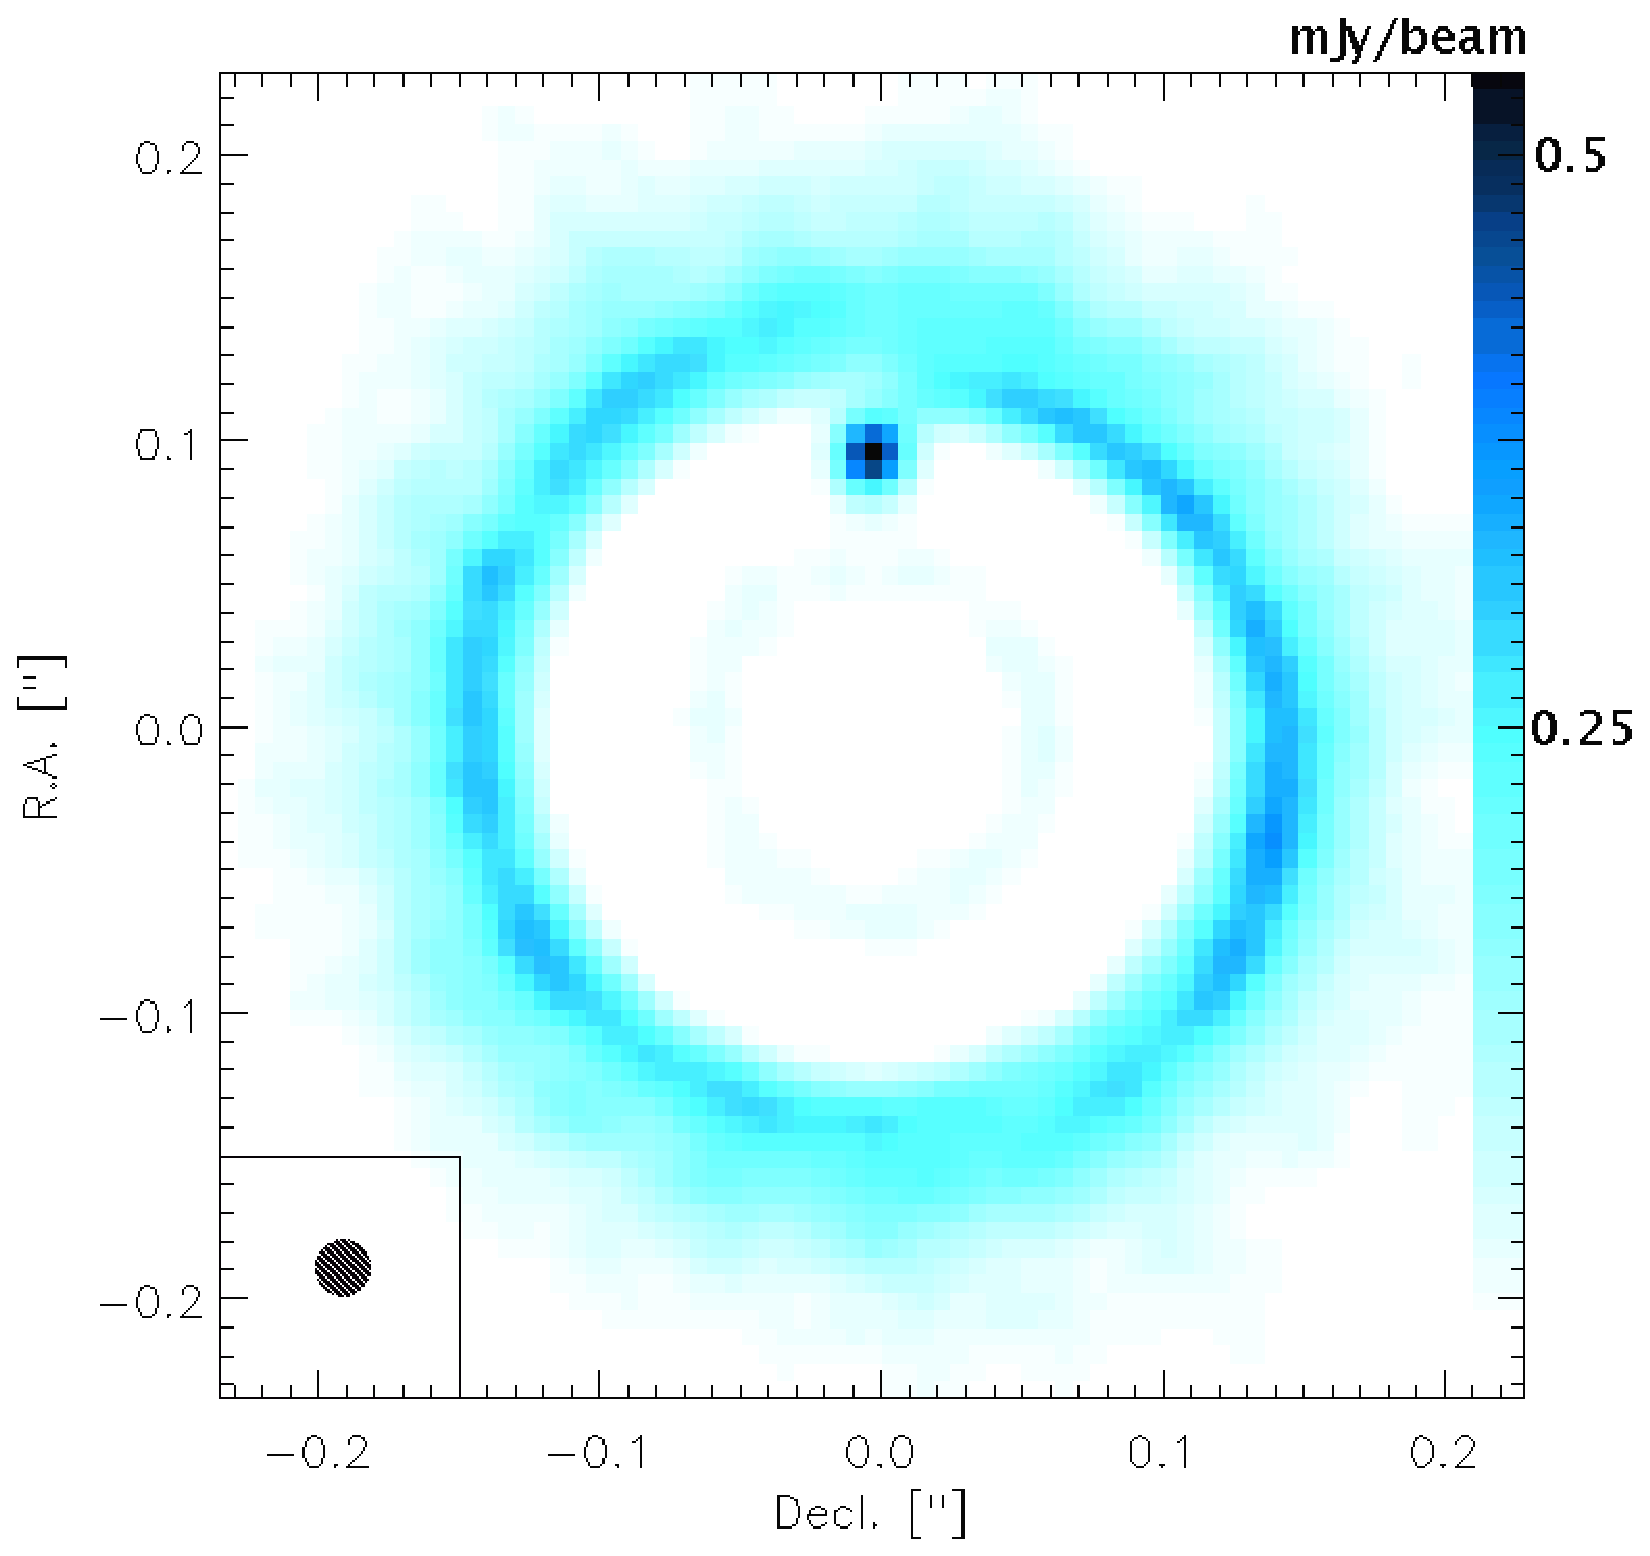
\includegraphics{d2fig1a.eps}}
    \hspace*{5mm}
%    \resizebox{0.45\hsize}{!}{\includegraphics{alma_100pc.eps}}
    \resizebox{0.45\hsize}{!}{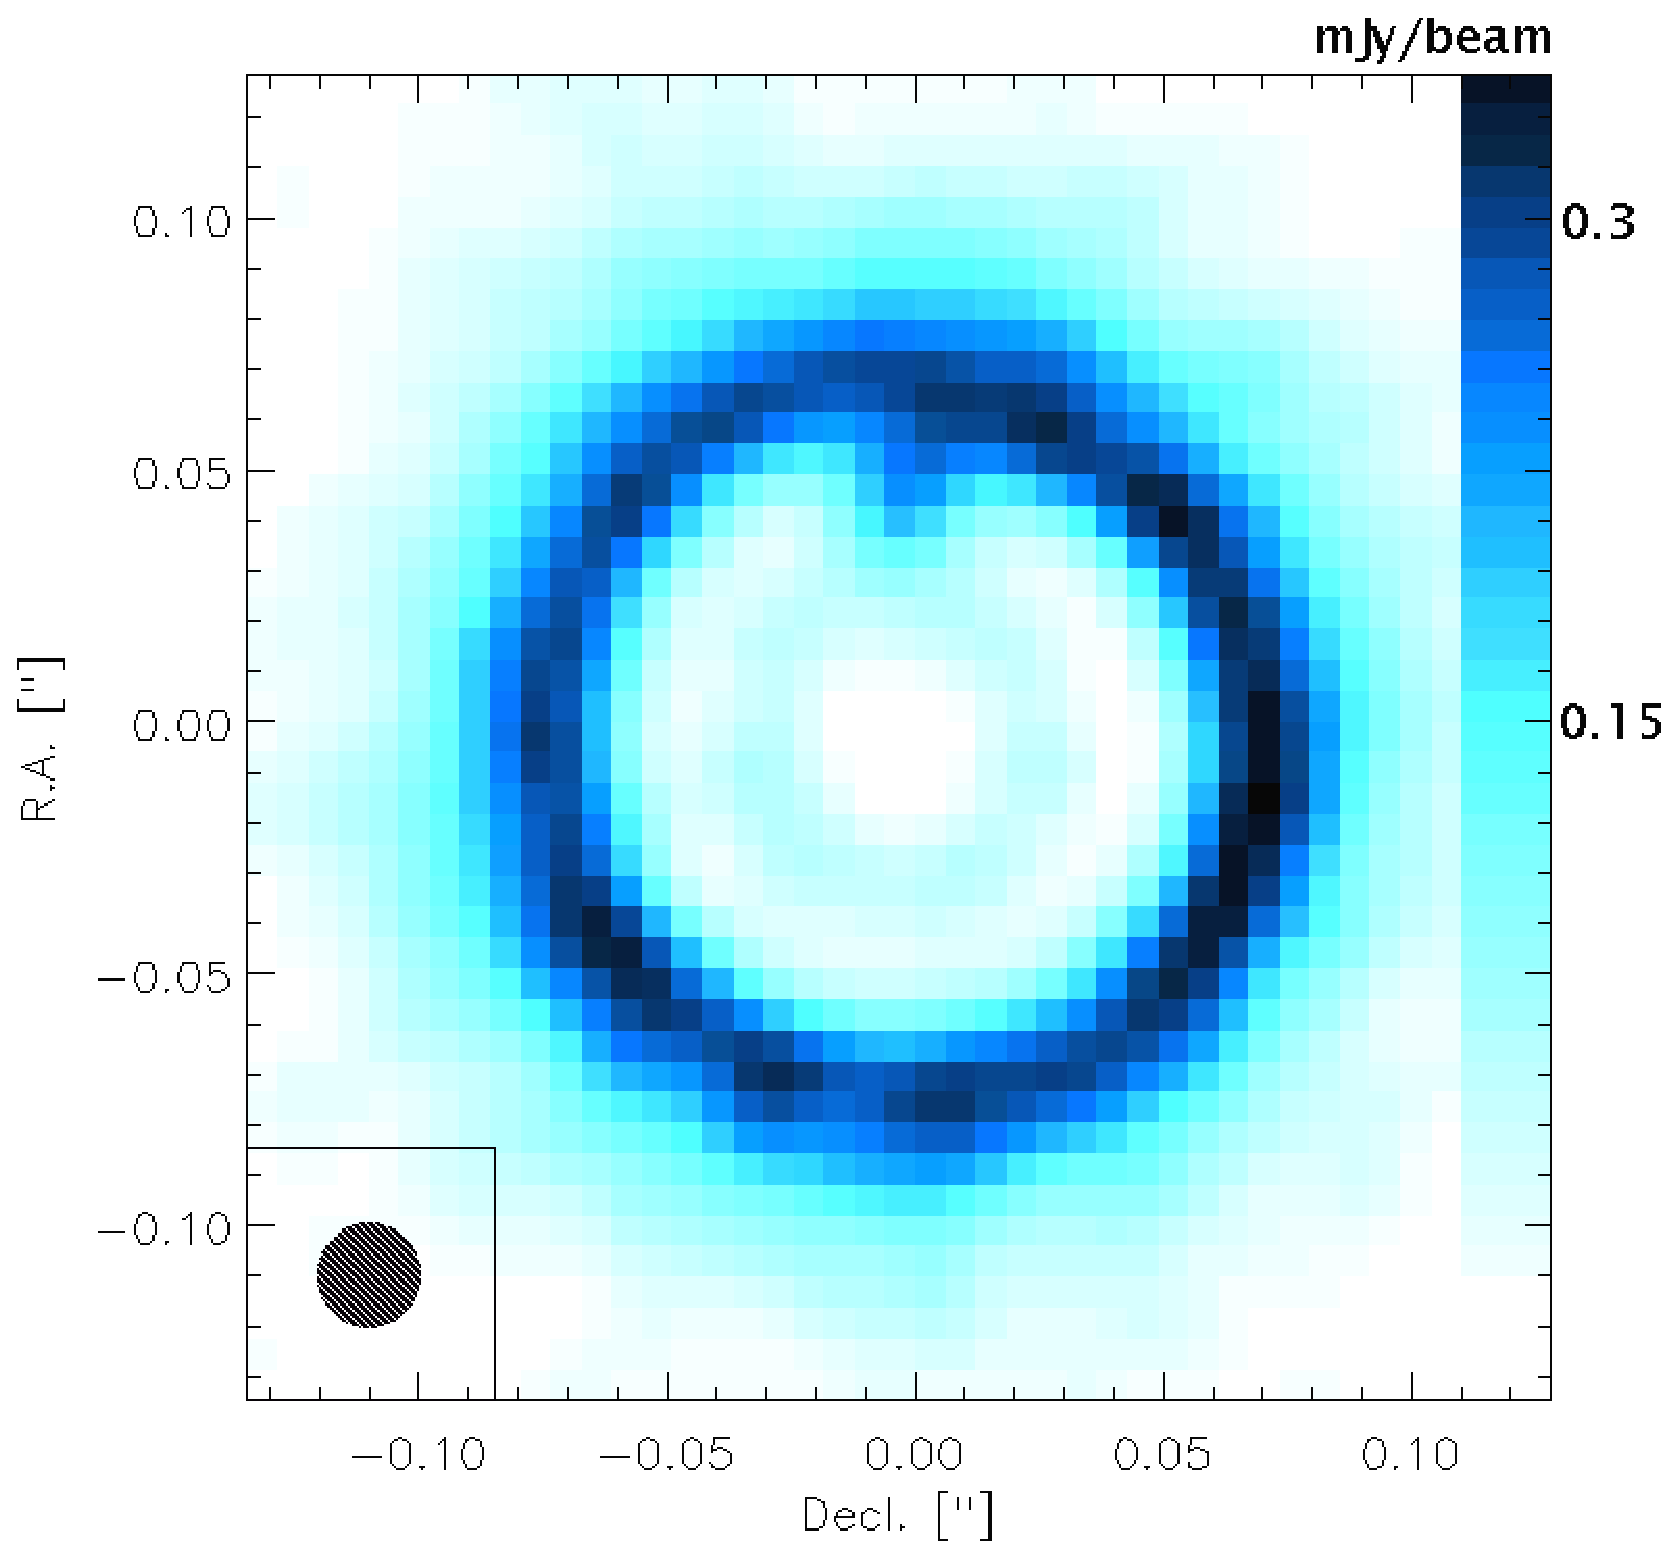
\includegraphics{d2fig1b.eps}}
  \end{center}
  \caption{Example for the application of the radiative transfer software {\tt MC3D}.
%    using hydrodynamic input data to make model predictions for telescopes, in this case {\em ALMA}.
    Here, a three-dimensional hydrodynamic model of a disk with an embedded planet with a mass of
    $1\,{\rm M_{\rm jup}}$ around a $0.5\,{\rm M_{\rm sun}}$ star (orbital
    radius: 5\,AU) has been used to investigate the feasibility
    to observe the planet and structures in the disk caused by the planet-disk interaction
    with {\em ALMA} (assumed distance is 50\,pc [left] / 100\,pc [right]).
%    The disk mass amounts to $M_{\rm disk} =
%    1.0\times10^{-2}\,{\rm M_{\rm sun}}$.  Only structures above the
%    $2\sigma$-level are shown.  
    The size of the combined beam is symbolized
    in the lower left edge of each image. Similar techniques will be
    used to derive observable quantities within the proposed project.
%    Note the reproduced shape of the
%    spiral wave near the planet and the slightly shadowed region behind the
%    planet in the left image.  
    {\em [from Wolf \& D'Angelo~2005]}
    \label{fig-giantplanet-alma}
    }
\end{figure}



%\noindent
%{\sl [a-2] Radiative transfer software in evolved, optically thin disks:} 
In addition to the {\tt MC3D} a radiative transfer tool was developed which
is optimized for the case of optically thin debris disks (Wolf \&
Hillenbrand~\cit{2005}).
%
% More specifically, it is optimized for studying arbitrarily structured,
% optically thin dust configurations where large grains (i.e., grains with a
% large size parameter) are expected to determine the far-infrared through
% millimeter dust reemission SED.  On the basis of optical properties of dust
% grains obtained through laboratory measurements, this software allows to
% derive scattered light and dust reemission SEDs for either analytically
% described dust density distributions or the direct implementation of the
% results of n-particle simulations.
%
This software has already been used in the context of theoretical studies
concerning the appearance of debris disks (Wolf \& Hillenbrand~\cit{2003};
Moro-Mart\'{\i}n, Wolf \& Malhotra~\cit{2005}) and for the analysis of
observed debris disk spectra (e.g., Sch\"utz et al.~\cit{2004}; Meyer et
al.~2004, Hollenbach et al.~2005; Kim et al.~2005;
Silverstone et al.~2006; Hines et al.~2006).

%We also have other radiative transfer tools available developed by the
%second PI. Of particular interest is a module for stochastic (quantum-)
%heating of very small grains and polycyclic aromatic hydrocarbons
%(Dullemond in prep.~{\bf XXXX}).
% This quantum module can, if necessary,
% also be built into {\tt MC3D}.


\subsection{Disk structure models}
%
Over the last years we developed various self-consistent models for the
structure of protoplanetary disks. Dullemond, Dominik \& Natta (\cit{2001})
presented a two-layer model similar to the model of Chiang \& Goldreich
(\cit{1997}), but with a treatment of the dust sublimation radius. They
argued that the dust inner rim (inward of which there is only gas, which is
presumably optically thin) is much hotter than the dusty disk behind it, and
is therefore presumably puffed-up. Moreover, we showed that the emission
from this inner rim can explain the near-infrared bump between 2 and 7
$\mu$m seen in nearly all Herbig Ae/Be star SEDs. We also developed more
detailed 1+1-D vertical structure models (Dullemond, van Zadelhoff \& Natta
\cit{2002}; Dullemond \& Natta \cit{2003a/b}), which are useful as a basis
on which calculations of the local physics can be done (e.g.~Kamp \&
Dullemond \cit{2005}). A final level of complexity was reached with models
based on 2D continuum radiative transfer (Dullemond \cit{2002}; Dullemond
\& Dominik \cit{2004a}). These models showed the possibility that the inner
regions of the disk might, under some circumstances shadow the outer disk regions
(in particular dust coagulation and sedimentation), causing these
to emit less strongly in the far-infrared. The discrepancy between the
flaring disks and the self-shadowed disks found in these models might
explain the different groups of SEDs observed for Herbig Ae stars (group I
and group II, Meeus et al.~\cit{2001}). 

We constructed models of dust sedimentation and coagulation which we
translated into observable features using a multi-dimensional radiative
transfer tool (Dullemond \& Dominik \cit{2004b}, \cit{2005}). The experience
gained in this work on coupling dust evolution models to radiative transfer
codes will be of direct use for the project proposed here.

Furthermore, we studied the effect of the disk formation and viscous evolution
history on the properties of disks observed at ages of typical T Tauri /
Herbig Ae stars. We have shown that the properties of the original core out
of which the star+disk system was formed may affect the level of
crystallinity of the dust in the disk (Dullemond, Apai \& Walch
\cit{2006}). We also show that such a simple model might explain the $\dot
M\propto M_{*}^2$ correlation observed in clusters (Dullemond, Natta \&
Testi \cit{ApJ, accepted}).

Depending on the goal we wish to address, these disk structure and 
evolution models will serve as a basis upon which radiative transfer
modeling will be performed in this project.

\subsection{Calculation of opacities and scattering properties of dust particles}
One of the crucial model parameters for the radiative transfer code outlined in Section~\ref{mc3d}
are the opacity and scattering properties (including the polarization of scattered radiation) 
of grains of various sizes and shapes. 
In this context, dust grains are in most applications considered to be spherical,
allowing to apply Mie theory.
In the particular case of circumstellar disks, broad grain size distributions
(grain radii $a$: nanometers -- millimeters)
and a very wide wavelength range ($\lambda \approx 10^{-10}-10^{-2}$\,m) of the interacting radiation have
to be considered. Previous numerical solutions to the Mie scattering problem are not appropriate to consider
size parameters $x=2\pi a/\lambda >10^4 - 10^5$.
In order to overcome this limitation, we developed a Mie scattering code which allows 
to calculate the optical properties of dust grains of arbitrary size (Wolf \& Voshchinnikov~2004).
Single scattering by particle ensembles is calculated by proper averaging of the respective parameters
(see also Wolf~2003b for a study of efficient radiative transfer in dust grain mixtures).
Furthermore, we have developed numerical algorithms for {\tt MC3D} which allow to consider
multiple light scattering in dust configurations containing aligned 
/ non-aligned non-spherical dust grains (Wolf et al.~2002b).


%spherical particles, Mie theory is often applied.  However, previous numerical
%solutions to the Mie scattering problem are not appropriate for particles
%that are very much larger than the wavelength of interest ($x=2\pi a/\lambda
%>10^4 - 10^5$). In disks with grain growth it is easy to get in this regime.
%In order to overcome this limitation, we developed a Mie scattering code
%which allows to calculate arbitrary size distributions / parameters (Wolf \&
%Voshchinnikov~\cit{2004}). Single scattering by particle ensembles is
%calculated by proper averaging of the respective parameters (see also
%Wolf~\cit{2003b} for a study of efficient radiative transfer in dust grain
%mixtures). 
%We have developed numerical algorithms for {\tt MC3D} (see [a-1]) which allow to consider
%multiple light scattering in dust configurations containing aligned 
%/ non-aligned non-spherical dust grains ().\\


% For reasons of simplicity dust grains are in most cases considered as
% homogeneous spheres in the modeling and interpretation of circumstellar
% disk observations.  However, in reality such particles and aggregates
% can have complex non-spherical structures
% 
% laboratory experiments of grain growth indicate
% that dust grains are expected to have a rather complex, possibly fractal
% structure 
% 
% (see Lumme \& Rahola~{\bf 1994} for porous dust particle light
% scattering).  Moreover, non-spherical grains are observed in star-forming
% regions through submillimeter polarimetry (e.g., Wolf, Launhardt \& Henning
% {\bf 2004}).  
% 
% In the optical to near-infrared wavelength range,
% non-centrosymmetric polarization patterns have been observed in bipolar and
% cometary nebulae (Scarrott et al.~1989), young stellar objects (Hajjar \&
% Bastien~1996), evolved stars (Kastner \& Weintraub~1996), and are also
% clearly seen in polarization maps of comets (Dollfus \& Suchail~1987).
% These findings as well as the wavelength dependence of the positional angle
% of polarization observed in red giants, AGB stars, and bipolar reflection
% nebulae (see, e.g., Johnson \& Jones~1991) and very high degrees of circular
% polarization of scattered light in the Orion molecular cloud, measured by
% Chrysostomou et al.~(2000), are considered to be caused by aligned
% non-spherical grains.  
% 
% \\
    


% ----------------------------------------------------------------------------------------
%\vspace*{5mm}
%\noindent
%{\bf [b] T Tauri Disk studies - Early Stages of Planet Formation}
%\vspace*{2mm}

%\noindent
\subsection{Deriving grain sizes from disk observations}\label{butter.model}
%{\sl [b-1] Dust grain evolution:}
We developed a radiative transfer model of the circumstellar environment of
the so-called ``Butterfly Star'' in Taurus (IRAS~04302+2247) - an edge-on
circumstellar disk (Wolf et al.~2003).  Our model is based on
multi-wavelength continuum observations: (1) Millimeter maps, and (2)
High-resolution near-infrared scattered light images obtained with {\em HST}/NICMOS.  The advantage
of the combination of both observations is that they trace (a) different
regions of the system and (b) different physical processes.  We find disk
and envelope parameters which are comparable with those of the circumstellar
environment of other young stellar objects. Most importantly, we find that the dust
properties must be different in the circumstellar disk and in the envelope.
While a grain size distribution with grain radii up to 100\,$\mu$m is
required to reproduce the millimeter observations of the disk, the envelope
is dominated by smaller grains similar to those of the interstellar medium.

Furthermore, we analyzed the $\sim$\,10\,$\mu$m silicate
feature of 27 T\,Tauri stars.  Here, we assumed that this emission
feature can be represented by a linear superposition of the
wavelength-dependent opacity describing the optical properties of spherical
homogeneous silicate grains with different chemical composition, structure,
and grain size. We show that acceptable fitting
results can also be achieved if emission properties of porous silicate
grains are considered instead.  We conclude that -- in terms of the
pro\-perties of the circumstellar dust -- T\,Tauri systems are a
continuation of HAeBe systems at their lower mass end (Schegerer et
al.~2006). 


% {\sl [b-2] On the observability of giant planets in circumstellar disks:}
% We investigate the possibility to detect giant planets that are still embedded in young circumstellar disks
% (Wolf \& D'Angelo~2005, Wolf et al.~2003).
% Based on models with different stellar, planetary, and disk masses, and different radial positions
% of the planet we analyze the resulting sub-millimeter appearance of these systems. 
% We find that the influence of the planet on the SED could not be distinguished 
% from that of other disk parameters. However, dust reemission {\em images} of the disks show that the hot region 
% in the proximity of a young planet, along with the gap, could indeed be detected
% and mapped with the Atacama Large Millimeter Array in the case of nearby circumstellar disks (d$<$100\,pc)
% in approximate face-on orientation (see Fig.~\ref{fig1}).
% \\




%\noindent
%{\sl [c-1] Structures in Debris Disks:}
%A software has been developed to simulate the dynamical evolution of dust particles in debris disks
%under the influence of stellar gravity, planetary perturbations, radiation and stellar wind forces (Rodmann~2005).
%It allows to determine the equilibrium density structure of dust in debris disks.
%\\
%
%\begin{figure}[t!]
%  \begin{center}
%    \resizebox{0.34\hsize}{!}{\includegraphics{f16.eps}}
%   \hspace*{10mm}
%    \resizebox{0.50\hsize}{!}{\includegraphics{f7a.eps}}
%  \end{center}
%  \caption{
%{\em [Top left]} 
%Possible degeneracy between the grain chemical composition and the 
%location of the planet clearing the gap. $\it{Solid~line}$: SED of dust disk 
%composed of MgSiO$_3$ grains with a 3M$_{\rm Jup}$ planet at 1 AU; 
%$\it{dashed~line}$: same for MgFeSiO$_4$ grains with a
%3M$_{\rm Jup}$ planet at 30 AU.
%{\em [Middle/Bottom left]}
%Brightness density distributions at 70 $\mu$m (assuming graybody emission from 
%12 $\mu$m grains) expected from a disk with a 3M$_{\rm Jup}$ planet at 1\,AU (middle) and 30\,AU (bottom), 
%respectively.
%{\em [Right]}
%SEDs of disks composed of 40$\mu$m grains with different grain
%chemical compositions, for a model resembling the solar system
%(i.e., the planets, excluding Mercury and Pluto, and the Kuiper belt
%as the source of dust; top right) and the corresponding debris disk without planets (bottom right).
%{\sl [from Moro-Mart\'{\i}n, Wolf \& Malhotra~2005]}
%  }\label{ama_deg}
%\end{figure}
%\noindent
%{\sl [c-2] Spectroscopic Signatures of Debris Disks:}
%In anticipation of future observations 
%of spatially unresolved debris disks with the Spitzer Space Telescope, we studied
%how the structure carved by planets affects the shape of the disk's SED 
%and consequently whether the SED can be used to infer the presence of planets 
%(Wolf \& Hillenbrand 2003; Moro-Mart\'{\i}n, Wolf \& Malhotra~2005).
%We numerically calculate the equilibrium spatial density distributions and SEDs of dust disks originated 
%by a belt of planetesimals in the presence of interior giant planets in different planetary configuration
%and for a representative sample of chemical compositions. The dynamical models are necessary to estimate 
%the enhancement of particles near the mean motion resonances with the planets and to determine how many particles 
%drift inside the planet's orbit. On the basis of the SEDs and predicted Spitzer colors we discuss what types 
%of planetary systems can be distinguished and the main parameter degeneracies in the model SEDs (see Fig.~\ref{ama_deg}).
%\\


% ----------------------------------------------------------------------------------------
%\vspace*{5mm}
%\noindent
%{\bf [c] Simulating the evolution of solids in protoplanetary disks}
%\vspace*{2mm}

%\noindent

\subsection{Simulating the evolution of solids in protoplanetary disks}
A code was developed to track the evolution of solids in protoplanetary disks
from the early phase when they are in the form of small dust particles, till
the stage when most of them are locked in a planetesimal swarm or have been accreted
onto the central star. A number of simplifications and idealizations allows
to consider gas-particle coupling, coagulation, sedimentation, and
evaporation/condensation processes. At the same time the code remains
computationally efficient allowing to calculate large grids of models and to
investigate how different properties of the protoplanetary disk influence
the architecture of the nascent planetesimal swarm
% Using another developed
% code that describes giant planets formation by core accretion gas capture
% model, it allows us to identify the disk parameters which are key in
% determining the properties of Jupiter-like planets 
(see e.g., Kornet \& Wolf 2006; Kornet, Wolf \& R${\rm
\acute{o}\dot{z}}$yczka~2006). This code can be used optionally, i.e.,
complementarily to the input from projects C1 and C2.


%\begin{figure}
%\centerline{\includegraphics[width=8cm]{myfig.eps}}
%\caption{This is the figure caption text....}
%\end{figure}

%
% Here follows the own refereed publications by the PIs in relation to
% the project proposed here.
%

\newpage
%\vspace*{2mm}
\ownpubltitle{Own publications related to the Forschergruppe:}
%
% BELOW IS ONLY AN EXAMPLE OF TWO ENTRIES. SEE THE ADDITIONAL FILES 
% SENT TO YOU WITH ALL THE REFERENCES FROM THE VORANTRAG
%
\begin{ownpubl}
\item Agol, E., Barth, A., Wolf, S. and Charbonneau, D. (2003)
  Spectropolarimetry and Modeling of the Eclipsing T Tauri Star KH15D, 
  \apj, {\bf 600}, 781

\item Carpenter, J., Wolf, S., Schreyer, K., Launhardt, R. and Henning,
  Th. (2005) Evolution of Cold Circumstellar Dust Around Solar-Type Stars,
  \apj, {\bf 129}, 1049

\item {Dullemond}, C.~P. and {Apai}, D. and {Walch}, S. (2006)
  Crystalline Silicates as a Probe of Disk Formation History, 
  \apjl, \textbf{640}, 67

\item {Dullemond}, C.~P. and {Dominik}, C. (2005) Dust coagulation in
  protoplanetary disks: A rapid depletion of small grains, 
  \aap, \textbf{434}, 971

\item {Dullemond}, C.~P. and {Dominik}, C. (2004b) The effect of dust
  settling on the appearance of protoplanetary disks, \aap
  \textbf{421}, 1075 

\item {Dullemond}, C.~P. and {Dominik}, C. (2004a) Flaring
  vs. self-shadowed disks: The SEDs of Herbig Ae/Be stars, \aap,
  \textbf{417}, 159

\item {Dullemond}, C.~P. and {Natta}, A. (2003b) An analysis of two-layer
  models for circumstellar disks, \aap, \textbf{405}, 597

\item {Dullemond}, C.~P. and {Natta}, A. (2003a) The effect of scattering on
  the structure and SED of protoplanetary disks, \aap, \textbf{408}, 161

\item {Dullemond}, C.~P. and {van Zadelhoff}, G.~J. and {Natta}, A.
  (2002) Vertical structure models of T Tauri and Herbig Ae/Be disks,
  \aap, \textbf{389}, 464 

\item {Dullemond}, C.~P. (2002) The 2-D structure of dusty disks around
  Herbig Ae/Be stars. I.  Models with grey opacities, \aap, \textbf{395}, 853

\item {Dullemond}, C.~P., {Dominik}, C. and {Natta}, A. (2001)
  Passive Irradiated Circumstellar Disks with an Inner Hole, \apj,
  \textbf{560}, 957

\item {Dullemond}, C.\ P. and {Turolla}, R. (2000) An efficient algorithm
  for two-dimensional radiative transfer in axisymmetric circumstellar
  envelopes and disks, \aap, \textbf{360}, 1187

\item Eisner, J.A., Hillenbrand, L.A., Carpenter, J.M. and Wolf, S. (2005)
  Constraining the Evolutionary Stage of Class I Protostars:
  Multi-Wavelength Observations and Modeling, \apj, {\bf 635}, 396

\item Hines, D.C., Backman, D.E., Bouwman, J., Hillenbrand, L.A., Carpenter,
  J.M., Meyer, M.R. et al.
%  Kim, J.S., Silverstone, M.D., Rodmann, J., Wolf, S.,
%  Mamajek, E.E., Brooke, T.Y., Padgett, D.L., Henning, Th., Moro-Martin, A.,
%  Stobie, E., Gordon, K.D., Misselt, K., Morrison, J., Muzerolle, J., Su,
%  K. 
  (2006) The Formation and Evolution of Planetary Systems (FEPS):
  Discovery of an Unusual Debris System Associated with HD 12039, \apj, in
  press

\item Hollenbach, D., Gorti, U., Meyer, M., Kim J.S., Morris, P., Najita,
  J., Pascucci, I., Carpenter, J., Rodmann, J., Brooke, T., Mamajek, E.,
  Padgett, D., Soderblom, D., Wolf, S. and Lunine, J. (2005) Formation and
  Evolution of Planetary Systems: Upper Limits to the Gas Mass in HD 105,
  \apj, 631, 1180

\item {Kamp}, I. and {Dullemond}, C.~P. (2004) The Gas Temperature in the
  Surface Layers of Protoplanetary Disks, \apj, \textbf{615}, 991 

\item Kim, J.S., Hines, D.C., Backman, D.E., Rodmann, J., Hillenbrand, L.A.,
  Moro-Martin, A., Carpenter, J.M., Silverstone, M.D., Bouwman, J., Mamajek,
  E.E., et al.
%  Meyer, M.R., Wolf, S., Malhotra, R., Pascucci, I., Najita, J.,
%  Henning, Th., Brooke, T.Y., Strom, S.E., Padgett, D.L., Stobie, E.B.,
%  Engelbracht, Ch., Gordon, K., Misselt, K., Morrison, J., Muzerolle, J.,
%  Su, K.Y.L. 
  (2005) Formation and Evolution of Planetary Systems: Cold Outer
  Disks Associated with Sun-like stars, \apj, 632, 659

\item Kornet, K. and Wolf, S. (2006)
  Radial distribution of planets. Predictions based on the Core Accretion / Gas Capture model for planet formation,
  \aap, in press

\item Kornet, K., Wolf, S. and R${\rm \acute{o}\dot{z}}$yczka, M. (2006)
  Planet formation around stars with various masses,
  \aap, in press

\item Meyer, M.R., Hillenbrand, L.A., Backman, D.E., Beckwith, S.V.W., Bouwman, J., Brooke, T.,Y., 
  Carpenter, J.M., Cohen, M., Gorti, U., Henning, Th., et al. (2004)
  \titl{The Formation and Evolution of Planetary Systems: First Results from a Spitzer Legacy Science Program},
  \apjs, 154, 422

\item Metchev, S.A., Eisner, J.A., Hillenbrand, L. and Wolf, S. (2005) 
  Adaptive Optics Imaging of the AU Microscopium Circumstellar Disk -- Evidence for Dynamical Evolution,
  \apj, {\bf 622}, 451

\item Moro-Mart\'{\i}n, A., Wolf, S. and Malhotra, R. (2005)
  Signatures of Planets in Spatially Unresolved Debris Disks,
  \apj, 621, 1079

\item Pascucci, I., Henning, Th., Steinacker, J. and Wolf, S. (2003)
  2D/3D Radiative Transfer Codes to Analyze and Predict VLTI observations,
  \textit{Astroph. \& Space Science}, {\bf 286}, 113

\item Pascucci, I., Wolf, S., Steinacker, J., Dullemond, C.P., Henning, Th., Niccolini, G., Woitke, P.
  and Lopez, B. (2004)
  The 2D Radiative Transfer Problem - Benchmark Results for Disk Configurations, 
  \aap, {\bf 417}, 793

%\item Rodmann, J. (2006) PhD thesis, University Heidelberg

\item Schegerer, A., Wolf, S., Voshchinnikov, N.V., Przygodda, F. and Kessler-Silacci, J.E. (2006)
  Analysis of the dust evolution in the circumstellar disks of T Tauri stars, 
  \aap, in press

\item Sch\"utz, O., Nielbock, M., Wolf, S., Henning, Th. and Els, S. (2004)
  SIMBA's view of the epsEri disk, 
  \aap, {\bf 414}, L9

\item Silverstone, M.D., Meyer, M.R., Mamajek, E.E., Hines, D.C., Pascucci, I., Hillenbrand, L.A., Bouwman, J., 
  Kim, J.M. et al.
%  Carpenter J.M., Stauffer, J.R., Najita, J., Moro-Martin, A., Henning, Th., Wolf, S., Backman, D.E., 
%   Brooke, T.Y., Padgett, D.L. 
  (2006)
  Formation and Evolution of Planetary Systems (FEPS): Primordial warm dust evolution from 3-30 Myr around Sun-like stars
  \apj, in press

\item Wolf, S. (2001a) 
  Dreidimensionaler Kontinuumsstrahlungstransport basierend auf der Monte-Carlo-Methode. Grundlagen und Anwendungen, 
  PhD thesis, Friedrich Schiller University Jena (Germany)

\item Wolf, S., (2001b)
  Inverse raytracing based on the Monte-Carlo method, 
  \aap, {\bf 379}, 690

\item Wolf, S. (2003a)
  MC3D - 3D Continuum Radiative Transfer, Version 2
  \textit{Computer Physics Communications}, {\bf 150}, 99

\item Wolf, S. (2003b)
  Efficient radiative transfer in dust grain mixtures, 
  \apj, {\bf 582}, 859

\item Wolf, S. and D'Angelo, G. (2005)
  On the Observability of Giant Protoplanets in Circumstellar Disks, 
  \apj, {\bf 619}, 1114

\item Wolf, S., Fischer, O. and Pfau, W. (1998) 
  Radiative transfer in the clumpy environment of young stellar objects, 
  \aap, {\bf 340}, 103

\item Wolf, S., Gueth, F., Henning, Th. and Kley, W. (2002a)
  Detecting planets in protoplanetary disks: A prospective study, 
  \apj, {\bf 566}, L97

\item Wolf, S. and Henning, Th. (2000)
  Accelerated self-consistent radiative transfer based on the Monte-Carlo method, 
  \textit{Computer Physics Communications}, {\bf 132}, 166

\item Wolf, S., Henning, Th. and Stecklum, B. (1999)
  Multidimensional self-consistent radiative transfer simulations based on the Monte-Carlo method, 
  \aap, {\bf 349}, 839

\item Wolf, S. and Hillenbrand, L. (2003)
  Model Spectral Energy Distributions of Circumstellar Debris Disks. 
  I. Analytic Disk Density Distributions, 
  \apj, {\bf 596}, 603

\item Wolf, S. and Hillenbrand, L. (2005)
  Debris disk radiative transfer simulator,
  \textit{Computer Physics Communications}, {\bf 171}, 208

\item Wolf, S. and Klahr, H. (2002)
  Large-scale Vortices in Protoplanetary Disks: 
  On the observability of possible early stages of planet formation, 
  \apj, {\bf 578}, L79

\item Wolf, S., Moro-Mart\'{\i}n, A. and D'Angelo, G. (2006)
  Signatures of Planets in Protoplanetary and Debris Disks, 
  \pss, submitted

\item Wolf, S., Padgett, D.L. and Stapelfeldt, K.R. (2003)
  The Circumstellar Disk of the Butterfly Star in Taurus, 
  \apj, {\bf 588}, 373

\item Wolf, S. and Voshchinnikov, N.V. (2004)
  Light scattering by very large grains, 
  \textit{Computer Physics Communications}, {\bf 162}, 113

\item Wolf, S., Voshchinnikov, N.V. and Henning, Th. (2002b)
  Multiple scattering of polarized radiation by non-spherical grains: first results, 
  \aap, {\bf 385}, 365

\end{ownpubl}
%

%\newpage
\section{Goals (Ziele)}\label{goals}

The general goal of this project is to provide a link between the results of
the laboratory and numerical experiments of this Forschergruppe and
astronomical observations of planetesimal-forming/harboring circumstellar
disks. In particular, the direct comparison of observable quantities
with existing or future observations will allow to verify the models for the different
phases of planetesimal formation derived by the other teams of the Forschergruppe.

Moreover, the goal is to identify the (combinations of) observable quantities which allow to trace the evolution
of the dust / disk in the potentially planetesimal-forming region 
(based on the simulation of the SED, spatially resolved, wavelength-dependent polarization and intensity maps 
in scattered and/or re-emitted radiation, and interferometrically observable quantities).
Based on the input from the projects A1, A2, B2, C1, C2, and D1, questions to be addressed,
mainly through parameter space studies, are\footnote{If certain questions rely on the input
from selected projects only, these projects are indicated in brackets. Otherwise, all projects apply.}

\begin{enumerate}

\item Is it possible to constrain the radial mixing efficiency traced by crystalline grains? [A1,A2]
  
\item To which extent can the vertical disk structure (as a function of the radial distance from the central star), 
  and thus the processes of dust settling, vertical mixing, and growth be constrained observationally? [A1,B2,C2]

\item Which complementary constraints about the size and structure 
  of dust grains can be derived from polarization measurements? [A1,B2,C2]
  
\item How do the observable quantities change during the early evolution of protoplanetary disks?
  (Rem.: The evolution will at first be parameterized by a decrease of the mass of submicron-sized dust grains.
  As a second step, the numerical description of the grain size distribution from project [\projdul{}]
  will be taken into account.)
  
\item What is the potential of combining spectrally resolved high spatial resolution imaging (milliarcsecond scale) 
  obtained in the mid-infrared wavelength range accessible from the ground (L,M,N,Q band) to significantly better
  constrain the chemical composition and size of dust grains than using the prominent $\sim$10\,$\mu$m 
  silicate feature alone? [A1,A2,B2,C2]
    
\item To which extent can the concentration of millimeter to centimeter-sized grains
  in anticyclonic vortices, spiral waves, and in/around turbulent eddies
  in the outer regions of protoplanetary disks be traced? [C1,B2]
  
\item Are short-term temporal variations on the timescale of years or less of any of the observable quantities expected 
  (particularly of those tracing the inner $<$\,1\,AU\,\ldots\,few AU planet forming regions of protoplanetary disks)?

\item Which infrared spectral signatures of protostars can be inferred from the early solar system mineralogy? [D1]

\item Which observations are needed to constrain the location of the snow-line traced by ices?
  
\item Which are the minimum / optimum requirements for the proposed observations, in terms of, e.g.,
  spatial resolution, wavelength range/coverage, spectral resolution, sensitivity, and accuracy?
  
\item What is the sensitivity / accuracy required to investigate the chemical composition of the smallest fragments
  resulting from planetesimal collisions in debris disks - as tracers for the chemical composition of planetesimals
  (taking into account the extremely low / undetected mid-infrared excess observed in the case of a significant fraction
  of debris disks with the Spitzer Space Telescope so far)?
  Which are the requirements for future space missions (using high-resolution imaging / nulling interferometry)? [A1,B2,D1]
  
\item What is the potential of combining near- to mid-infrared spectra obtained from space missions,
  tracing the global disk appearance,
  with spatially resolved interferometric observations of the planet forming region, obtained from the ground,
  but with a much more restricted wavelength-coverage?
  
\item What is the potential of spectro-interferometric observations with the VLTI in terms of constraining
  the dust evolution, using the current and planned 2$^{\rm nd}$ generation instrumentation in different wavelength regions
  (tracing scattered vs.\ re-emitted radiation)? The results of this study will have direct impact on the
  science case studies for the 2$^{\rm nd}$ generation interferometric instruments MATISSE and VSI
  (Remark: The PI of this project is Project Scientist/Co-PI of MATISSE and Member 
  of the science team of the VLTI Spectro-Imager [VSI]).
\end{enumerate}

In order to address these questions (and those resulting from these studies),
a flexible radiative transfer modeling setup will be developed, based on the profound
preliminary work outlined in Section~\ref{prelim}.
The basis for this will be a disk model, implemented in the radiative transfer simulation tool {\tt MC3D}, 
with following specifications:
\begin{itemize}  
\item The model shall allow a detailed analysis of the dependence of observable quantities on
  the radial and vertical distribution of 
  a) the size distribution and
  b) the chemical composition and structure of dust grains.
  In particular, porous grains (important for the earliest stage of growth), 
  ice-mantled grains, and PAHs have to be considered.
\item Self-consistent solution of the vertical disk structure and the sublimation region of dust grains / ice mantles on grains
  (depending on the radial and vertical location in the disk).
%\item For the extension of the investigation towards more evolved disks, the effects of
%  radiation pressure, Poynting-Robertson effect, and the effect of photophoresis are to be considered in a self-consistent manner.
\item Similar to previous studies (see Section~\ref{mc3d}) software interfaces have to be developed which allow
  to implement 
  a) the optical properties derived in project A1 and
  b) the density and grain size distributions from projects A2, B2, C1, C2, and D1.
\end{itemize}

%A flexible radiative transfer modeling setup will be developed that
%will allow us to test the observational effect of various results from the Forschergruppe.
%Conversely, with this setup we will explore which aspects of
%the growth process from dust to planetesimals might be responsible for
%certain well-known observational facts of protoplanetary disks such as the
%existence of large inner holes, the existence and radial abundance
%variations of crystalline silicates, the observed grain sizes etc. .

%The particular goals to be targeted are the following:
%\begin{enumerate}
%\item \label{goal-c2} Constrains on grain size distributions and grain growth
%  in young gas-rich disks, in close collaboration with C2, with additional
%  input from projects C1, B2 and B4. From the model toward the observations,
%  we intend to:
%  \begin{enumerate}
%  \item Put constraints on processes of dust settling, vertical mixing
%    and growth from direct and indirect observations of the disk
%    geometry and vertical structure. For this we will use both infrared
%    spectral energy distributions as well as imaging.
%  \item Set limits on radial drift of dust by comparing models with
%    different radial drift efficiencies to observations.
%  \item Identify ways in which the study of observable dust grains
%   ($a\lesssim 1$ mm) in protoplanetary disks by infrared and
%   (sub-)millimeter telescopes provide clues to the {\em unobservable}
%   process of growth from $a\sim 1$ mm to multi-kilometer
%    planetesimals.\label{dulgoal-linkobs}
%  \item Identify ways in which the observable grains in the {\em surface
%    layers} of the disk provide clues to the unobservable grains {\em
%    deeply embedded within the disk}.
%  \end{enumerate}
%  Conversely, there are well-known recent observational peculiarities of
%  disks observed, which we intend to address by putting them in the 
%  context of the models:
%  In addition to this we will attempt to solve some of the observational
%  mysteries listed above using the combination of the coagulation and
%  radiative transfer models.
%  Of these above observational aspects we will fully address only those for
%  which we, in the course of the Forschergruppe, find possible explanations
%  in terms of the research of this Forschergruppe and/or earlier known
%  physics.
%\item \label{goal-d1} A mineralogical comparison between the solar system
%  and protoplanetary disks, in close collaboration with project D1:
%  \begin{enumerate}
%    \item Comparison of mineralogical composition of Calcium-Aluminium-rich
%      Inclusions (CAIs, i.e.~the oldest components of meteorites originating
%      from undifferentiated planetesimals) with the mineralogy of
%      protoplanetary disks as derived from infrared spectroscopy.
%    \item Search for water-alterated minerals (phyllosilicates) in 
%      protoplanetary disk infrared spectra, as a hint for the presence of
%      large planetesimals in young gas-rich disks. 
%    \item {\bf MARIO: Are there other ways by which one could check
%      for planetesimals? Perhaps check for typical minerals in 
%      differentiated planetesimals? Basalts? What would such minerals
%      look like?}
%    \item In general: search for new minerals in the infrared spectra
%      of protoplanetary disks, based on minerals found in meteorites.
%  \end{enumerate}
%\item \label{goal-a2} Constraints on radial mixing of minerals from infrared
%  observations of protoplanetary disks, in close collaboration with project
%  A2. Insert model predictions of mineral abundances as a function of radius
%  from project A2 into the radiative transfer model to predict:
%  \begin{enumerate}
%    \item infrared spectra of the full disk and compare to e.g.~Spitzer
%    Space Telescope spectra.
%    \item infrared spectra {\em as a function of radius} and compare with
%      data from the VLT-MIDI interferometer and the VLT-VISIR camera.
%  \end{enumerate}
%  Derive constraints on the solid-state chemistry in disks and on the radial
%  mixing efficiency of the turbulence in the disk (the Prandtl number).
%\item Constrains on the location of intermediate-size bodies in 
%  gas-poor final stages of disks (debris disks).
%\item Investigate instrumental requirements, observational conditions and
%  feasibility of the above mentioned observations. Identify (and study the
%  feasibility of) potential new ways in which current/future observational
%  techniques (and combinations thereof) can be linked to the results from
%  the Forschergruppe. For instance:
%  \begin{enumerate}
%  \item Mineralogical analysis of {\em debris disks} using infrared
%    spectroscopy. Since this dust arises from planetesimal collisions {\em
%    only}, this allows us to `get a look inside' of planetesimals around
%    other stars.  Is such a study feasible in the light of the very weak
%    infrared excess of debris disks? If so, do they consist of similar
%    materials as the meteorites from our own solar system?
%  \end{enumerate}
%\end{enumerate}



\section{Work schedule (Arbeitsprogramm)}

\subsection{Methods}\label{methods}
The key task of this project is to derive observational constraints for the
evolution of solids in circumstellar disks. Both the initial conditions
(submicron-sized dust grains) and early evolution of these solids (growth
via coagulation to $\sim$\,mm-sized particles) can be observed directly in
the optical to millimeter wavelength range. Bodies larger than $\sim$1\,cm
cannot be traced directly.  However, these bodies of centimeter to
planetesimal size strongly influence the small grain population -- a
population which dominates the appearance of disks through their entire
evolution.  This is because collisions of larger bodies create fragments
which allow to trace the location, abundance, and chemical composition of
the cm to $\sim$ few km sized parent bodies. 
Possibilities to probe these larger bodies
indirectly will be investigated by combining detailed models of the growth and fragmentation processes 
-- studied in the various Forschergruppe projects -- with detailed radiative transfer tools. 
Very large bodies (planets) also affect the dust population by their
gravity. This can be very important for the structure and thus the appearance of disks,
but we will account for this only if it is essential for particular questions
because the Forschergruppe is focused on bodies up to a few hundred kilometers in size only.

We will consider various kinds of observations to trace the size distribution of the particles in the disk
as well as the mineralogical composition. As outlined before, the main analysis tool will be a radiative 
transfer tool set which allows the easy insertion of results from the Forschergruppe as input
physics, and therefore allows a direct link between experiments and models 
on the one hand and observations on the other hand.

%Since we wish to address many different issues (linking as much as possible
%the Forschergruppe to observations), it will be essential to consider a
%broad range of telescopes and instruments for which there is already a
%large volume of archival data and/or for which we have collaborations with
%teams which have access to such data. Here is a list of telescopes and 
%instruments which are useful/important for our project, and why:
%\begin{itemize}
%\item[{\em Spitzer-IRS:}] The Infrared Spectrograph on board the Spitzer
%Space Telescope yields the most sensitive infrared spectroscopy to date, in
%the range of 5 - 38 $\mu$m. Archival data exists for Herbig Ae/Be stars
%({\bf XXXXX}), T Tauri stars (e.g.~Kessler-Silacci et al.~\cit{2006}) and
%even a number of Brown Dwarfs (Apai et al.~\cit{2006}). This wavelength
%ranges covers the 10 $\mu$m Si-O resonance feature of silicates, including
%the peaks of various crystalline silicates such as forsterite, enstatite,
%all of which have been identified in such spectra already. The range between
%20 and 38 $\mu$m contains various bands of forsterite at lower temperatures,
%probing the somewhat more outer regions of the disk, where the presence of
%such crystals is closely linked to theories of radial mixing (project A2).
%The entire spectral range also covers potential peaks of the various
%minerals identified in meteorites (see Fig.~{\bf XXXXXXX}). The second PI
%is member of the Spitzer Legacy Team ``cores to disks'', and therefore has
%access to high-quality reduced data for hundreds of protoplanetary disks.
%\item[{\em VLT-MIDI:}] The MIDI instrument on the Very Large Telescope is a
%mid-infrared interferometer, allowing to obtain 8-13 $\mu$m spectroscopy
%{\em as a function of distance from the star}, basically resolving from
%$\sim$1 AU out to $\sim$20 AU for disks at typical distances to Earth. Since
%the 10 $\mu$m feature shape tells about the size and composition of the
%dust, this can be directly linked to theories of radial mixing, as well as
%theories of grain growth, sedimentation and vertical mixing. MIDI has been
%built at the Max-Planck-Institute for Astronomy, there is excellent access
%to high-quality data. A follow-up of MIDI, called MATISSE, is in planning.
%The first PI of this proposal is Project Scientist/Co-PI of MATISSE and
%Member of the science team of the VLTI Spectro-Imager [VSI].
%\item[{\em VLT-VISIR:}] VISIR on the Very Large Telescope is a spectrograph and
%imager in the N and Q-band (8-13 $\mu$m and 16.5-24.5 $\mu$m), with the
%diffraction-limited spatial resolution of the 8-meter single VLT
%telescope. For disks at typical distances one can resolve down to 
%about 20 AU distance from the central star, complementing the resolving
%power of VLT-MIDI.
%\item[{\em Optical imaging:}] {\bf Sebastian: polarimetry?? here I have very
%little knowledge} {\bf LINC-NIRVANA?}
%\item[{\em Millimeter observations:}] With various telescopes (Plateau de
%Bure; Very Large Array) a number of authors have obtained (sub-)millimeter
%maps of the outer regions of disks ($\gtrsim$ 50 AU) looking for evidence of
%large ($\gtrsim$ 1 mm) grains in these regions ({\bf XXXX}). It is the only
%current method of obtaining direct evidence for grains in the mm and cm size
%regime (direct evidence for larger grains is impossible), albeit only in the
%outer disk regions. Data available in the literature.
%\item[{\em Future: SOFIA, HERSCHEL:}] The SOFIA telescope on board a
%Boeing 747 is expected to fly within the next few years. The
%SAFIRE-spectrograph covers 145 - 655 $\mu$m, which is important for 
%obtaining the SEDs of disks (i.e.~hints on the disk geometry). In the
%somewhat more distant future the
%HERSCHEL Space Telescope will fly with the PACS instrument on board
%(in which MPIA has a part in the development), which covers 57-210 $\mu$m.
%This wavelength range includes many features of minerals contained in
%meteorites (see figure {\bf XXXX}) {\bf MARIO: PLEASE CHECK!}, and we
%can make predictions for this instrument.
%\item[{\em Future: ALMA:}] The Atacama Large Millimeter Array will, when
%on-line, be able to probe the distribution of grains with sizes up to
%millimeters throughout the disk. The spatial resolving power will allow
%to detect clumpiness or the concentration of grains in spiral waves. These
%are both features that are predicted by theory, in particular in project
%C1. In collaboration with C1 we can therefore predict what kind of
%patterns ALMA might find.
%\end{itemize}

\vspace{1em}
\noindent{\bf\em Modeling tools:}\\
\noindent 
In the framework of the proposed project various numerical methods will have
to be applied (see Section~\ref{prelim} for a more detailed description):

\begin{enumerate}
\item {\em Continuum radiative transfer calculations}\\
%
To derive observable quantities from the results of the Forschergruppe a
multi-dimensional radiative transfer code is required. The PIs of this
project have profound experience in the field of the development and
applications of radiative transfer codes, in particular in the field of
circumstellar disks. Although the PhD student will primarily apply existing
radiative transfer tools, necessary improvements of these are part of the
project as well. 

We will use the three-dimensional continuum radiative transfer code {\tt
MC3D} to compute spectra, wavelength-dependent intensity and polarization
maps, and derived quantities (such as interferometric visibilities).  This
software is highly flexible, allowing to adapt all relevant parameters of
the dust/disk model, such as the dust density distribution in the disk, the
optical properties of an arbitrary number of dust species, the grain
size distribution, etc.\,.  It is well-tested and has been applied for
similar purposes earlier (see Section~\ref{prelim}).

%Additions to the code, to be developed within this project:
%\begin{itemize}
%\item 
For modeling disks with very small grains, stochastic (quantum-)
heating has to be taken into account. The second PI has a module for
quantum-heated grains in his radiative transfer code {\tt RADMC}.  Since for
practical reasons we intend to use a single code in this project, rather
than switching between codes, we plan to implement this module into the
{\tt MC3D} code.
%\item To enable quick interactive modeling, we intend to parallelize the
%code using a very simple trick: instead of one run with, say, $10^7$ photons
%we will do 100 runs with $10^5$ photons, and average the resulting
%temperature profiles in a suitable way. This cheap method of
%parallelization, which requires no extra changes to the program, will be
%implemented and tested.
%\end{itemize}

\item {\em Codes for computing the opacity and scattering properties of
grains/aggregates}\\
%
Since we wish to study disks in which grain growth has possibly proceeded to
very large sizes, we will calculate the opacities and scattering properties
of the grains using a special Mie code developed by Wolf \& Voshchinnikov~(2004).
This code is able to treat grains with sizes well beyond $10^4$ times
the wavelength of interest. For treating grains with ice mantels and/or
porous structure we will use codes which are available to the team through
collaboration with N.V.~Voshchinnikov. 

Certain aggregation mechanisms, however, tend to yield very `fluffy'
(fractal) aggregates (e.g.\ Kempf et al.~1999). 
%The opacity of such
%aggregates is notoriously difficult to calculate. 
Min et al.~(2006) computed opacities of fractal grains using the Discrete Dipole
Approximation, and have shown that the opacity of large fractal grains with
low fractal dimension still looks like that of their much smaller
constituent particles. They propose an equivalent homogeneous and equivalent
porous grain who's opacity (at least in the 10 $\mu$m feature) is equivalent
to that of the bigger fractal grain. This is one of the possible ways 
in which the fractal structure of aggregates can be included in the models.

\item {\em Disk density structure and evolution models}\\
%
A radiative transfer tool can only predict spectra and images for a disk of
which the density structure is known beforehand. We have multiple years of
experience in self-consistent disk structure- and evolution model
development (see Section~\ref{prelim}). This experience, and the available
1+1D and 2D disk structure model tool sets, will provide the basis of the
models of this project. In principle, projects A2 and C1 will also yield
full-fledged disk structure models which can serve as the basis of the
radiative transfer calculations, but for flexibility we will also have our
own models available.
\end{enumerate}

\vspace{1em}
\noindent{\bf\em Observations:}\\
\noindent Considering the wide field of the intended comparisons of the
Forschergruppe results to observations we will, for a large part, rely on
archival data.  In addition, we will outline future observation strategies
to be followed for addressing particular issues.
However, in particular in the advanced stages of
the project (year 2 and 3), we keep the possibility open of writing
dedicated observing proposals and
analyzing them with the modeling tool set developed in this project.


\vspace{1em}
\noindent{\bf\em Interfacing with projects A1}\\
\noindent 
%
The optical properties of dust grains derived from annealing experiments
will be considered in studies of the evolution of dust grains in the innermost regions of young circumstellar disks.
In combination with the density distribution of the various dust species derived
from radial mixing simulations (project A2), the feasibility to quantify the processes of annealing and mixing
observationally will be investigated. 
However, before implementing the results from project A2 (in the second half of the project), we will
use a parameterized approach in order to investigate the parameter space as completely as possible.


\vspace{1em}
\noindent{\bf\em Interfacing with projects A2 and C2:}\\
\noindent 
%
Projects A2 and C2 give the abundances of various species and sizes of
dust/dust-aggregates at each position in the disk. 
%For the sizes these
%projects deliver the size distribution of the grains. 
For $N$ dust species, and a discretized size distribution in $M$ size-bins, this yields $N\times
M$ dust abundance values at each spatial grid point. Since the runtime of the radiative
transfer is correlated with the number of abundances per spatial grid point,
we will determine the minimum number of required size bins which can still correctly reproduce the
outcoming infrared spectra. Any output from A2 and C2 will then be mapped
onto that reduced size-grid to save computing time for the radiative
transfer. In this way a direct link from A2 and C2 to the observations
can be established. 

%However, since the models of A2 and C2 are likely rather heavy, 
In order to allow a flexible investigation of the parameter space, 
we will also follow approximation strategies:
\begin{itemize}
\item Taking simple parameterized models of the grain size distribution
as a function of position in the disk, as well as the mineralogical
composition of the grains to get a rough qualitative understanding for
the kind of distribution which fits the observations best.
\item Devising simple parameterized `fits' to the complex model results.
\end{itemize}

The main output of A2 relevant to this project is expected to be the
abundance {\em as a function of radius} of crystalline forsterite and
enstitate, as well as pyroxene, olivine, quartz etc.\ . These abundances
will depend on conditions in the disk (see project A2), and thus, by
comparing these outcomes via the radiative transfer to observations we can
put constraints on these conditions.

%The main output of C2 relevant to this project is the grain size
%distribution of the observable dust at each location in the disk, possible
%also with information about the {\em structure} of the aggregates 
%(compact, porous, fractal). 

% On top of
% these models we will be able to vary the abundance of various dust species
% and sizes, according to the output of projects, A2, B1-B4, C1 and C2. And
% to make analysis of observations easier we will also parameterize these
% abundances and derive constraints on these parameters.

\vspace{1em}
\noindent{\bf\em Interfacing with project C1:}\\
\noindent 
%
For the prediction of clumpiness in (sub)millimeter images of current-day
instruments and future observations, e.g.\ with {\em ALMA}, we need predictions / constraints concerning the
concentration of particles in density perturbations in the disk.  This is
one of the expected output results from project C1. From those simulations we
will import the density of solids as a function of the position in the disk,
and hence we require 3D radiative transfer calculations for this. {\tt
MC3D} is an ideal tool for this and has already been used multiple times to
predict images and spectra from 3D hydrodynamic density distributions 
(Wolf et al.~2002a, Wolf \& Klahr~2003, Wolf \& D`Angelo~2005). 
Since grains of a rather specific size (at 100\,AU about
millimeter to centimeter size, for typical gas densities) are most likely to be trapped in
density perturbations, while much smaller and much bigger particles do not
feel this trapping force, we will perform simulations with the concentrated
particles from project C1 {\em coexisting with} a more homogeneous
distribution of small particles (not modeled by C1; we will use a
homogeneous abundance for this). This way we can determine whether the
concentrations of millimeter to centimeter size particles residing near the disk midplane
will still be visible if they are embedded in a flaring disk consisting of
large amounts of additional (homogeneously distributed) small dust. We will
determine observational requirements for detecting such concentrations / density inhomogeneities.


%Since the gas in the disk is expected to be removed by photoevaporation
%leaving behind the bigger grains (Throop et al.~2001), C1 will also
%do models at much lower disk gas densities, for which the concentrated
%particles have a smaller size. We will investigate if it will be possible with ALMA 
%to derive the typical grain size of concentrated particles, and if
%so, whether one can derive the local gas density from this. This would
%be a new method of deriving the mass of the disk. 




%In
%many cases infrared opacity curves for minerals found in meteorites have
%already been acquired. 
%By analyzing the composition
%of CAIs, {\bf XXXX} have been able to predict the infrared spectral features
%of dust in very young protoplanetary disks, because CAIs are thought to
%originate from the earliest dust in the protoplanetary disk ({\bf XXXX}).
%The material in chondrules and matrix in meteorites has been aqueously
%altered {\bf [*** MARIO, PLEASE CHECK ***]}. Since liquid water is expected
%only on planetesimals of considerable size, these materials must have been
%produced in earlier planetesimals {\em prior} to being incorporated in the
%parent body of the meteorite {\bf [*** MARIO, PLEASE CHECK ***]}.  Also of
%these minerals the infrared opacity tables are available (provided by the PI
%of project D1), and will be measured in project A2. The unambiguous
%detection of signatures of these minerals in the infrared spectra of
%protoplanetary disks would therefore indicate the presence of large
%planetesimals in these disks. This would set strong time limits on the
%formation times of these bodies, which can be compared with the time scales
%measured using short-lived nuclides in project D1.



\vspace{1em}
\noindent{\bf\em Interfacing with projects D1}\\
\noindent 
%
%IR spectral signatures of protostars inferred from early solar system mineralogy
The abundance of minerals in the early solar system can be inferred from primary relics in meteorites or theoretical considerations of condensation sequences at early solar system conditions. Dust reemission spectra can be calculated that would be expected for the early solar nebula, and compared to protoplanetary disks. Such a comparison will enable us to further place our solar system in context, and possible differences will probably hint at different evolution paths and possible reasons. Up to now, only Mg-rich silicates (forsterite, enstatite, crystalline and amorphous) are considered to fit protoplanetary disc spectra. For the early solar system, we expect differences mainly due to I) Ca, Al rich minerals and II) hydrous silicates. 
The exact magnitude of the characteristic features of the minerals mentioned above will be modeled with radiative transfer calculations, based on mineral abundances calculated in project A2, and observational constraints from D1.


%I) Ca,Al rich inclusions (CAIs) reflect the inventory of minerals that condense at highest temperatures: Corundum, hibonite, spinel, melilite, Ti-rich diopside (fassaite), anorthite. Relevant - as most abundant - are melilite, Ti-rich diopside and spinel, and they have IR absorption features that readily allow their distinction form Mg-silicates (olivine and pyroxene solid solution, particularly forsterite and enstatite). Although Ca,Al rich silicates and oxides should be less abundant (about a factor of 4, if elements occur in solar/cosmic proportions) than Mg-silicates (if the latter are condensed), Ca,Al minerals could be detectable in inner disks where temperatures are in excess of forsterite and enstatite condensation temperatures, or in cases where Mg-silicates are amorphous or not too abundant. Most characteristic features (distinguishing them from Mg-silicates) are expected at 14-15 $\mu$m (spinel) and 50-70 $\mu$m (melilite, diopside), and could be searched for by MIDI (or VISIR?) close to the central star, or by Spitzer and Herschel, in order to get upper limits on their abundance.

%II) As well promising seems a search for hydrous silicates which are abundant in our solar system: about 50\% of interplanetary dust are hydrous silicates, many carbonaceous chondrites have them. This dust is debris dust, as hydrous silicates formed by aqueous alteration of former anhydrous minerals on asteroids that were heated due to decay energy provided by short-lived nuclides (26Al) in the early solar system. Thus, the presence of hydrous silicates in protoplanetary discs would also indicate the early presence of larger bodies with liquid water inside, and their collisional destruction. Hydrous silicates such as serpentine, chlorite, or montmorillonite (for smectite there are no data yet) have characteristic IR features (distinguishing them from Mg-silicates) at 9 um, and between 70-100 um, and could be observed with Spitzer and/or Herschel. Although Bouwman et al. (2006) did not detect such signatures in a Spitzer survey of Herbig Ae stars, this could be just due to the fact, that these discs formed in low mass star regions: here no massive evolved stars are present that could inject short-lived nuclides into these discs, so planetesimals are not subjected to heating and aqueous alteration. However, future studies of solar-mass discs in regions with massive evolved stars are planned, and here the conditions could be very different, favoring the early presence of hydrous silicates in significant abundances.

%Another mineral expected at low condensation temperatures is FeS, and has also characteristic IR features that could be searched for.



% -----------------------------------------------------------------------------------------------------------------
\subsection{Schedule}

\subsubsection{First year}

In the first 6 months the student will learn how to use the existing modeling equipment.
%that he/she will use. 
%The student will experiment with the poor-man's
%parallelization trick outlined above, and see if it works properly and
%efficiently. In this period the work will be mainly of exploratory nature,
%and the student will read him/herself into the existing literature. 
In particular, the student will learn how to estimate the
feasibility of certain kinds of observations with existing or near-future
observational instruments.
%In the second half year we will address goal \ref{goal-d1}: the
%mineralogical comparison of the solar system to protoplanetary disks.
%Laboratory spectra for mineral mixtures extracted from meteorites are
%already available in the literature, and the laboratory of Pucci can, upon
%request, quickly provide additional measurements if needed. This sub-project
%is also simple enough as a starting project. In detail:
%\begin{itemize}
%\item Using analytic methods similar to van Boekel et al.~({\bf XXXX}) and
%  Schegerer et al.~(\cit{2006, our team}) we will hunt for signatures of
%  these minerals in available Spitzer spectra (collaboration with Bouwman
%  for Spitzer spectra of Herbig stars; archival data for the spectra of T
%  Tauri stars).
%\item Since these signatures might be very weak, we will -- if necessary --
%  study correlations between spectra of many sources, to see if certain
%  signals are clearly different from noise. Care will be taken to see that
%  signals do not lie on top of order-boundaries of the IRS instrument, which
%  could give spurious peaks.
%\item Estimates will be made, based on this experience, whether
%  phyllosilicates or other minerals of interest might be detectable in
%  debris disk spectra with current or planned future instruments.
%\end{itemize}
Besides this, the project is focused during the first year on the development and
application of a state-of-the-art model for the dust phase of
circumstellar disks (see Section~\ref{goals}) which will serve as the basic tool
for the subsequent studies.  A parameter study, based on
existing grain growth / planetesimal formation scenarios and optical
properties of the dust shall be completed during the first half of the second year.

\begin{itemize}
\item Development of a model set for young circumstellar disks as outlined
  in Section~\ref{goals}.  
  Development of the required software interfaces which allow to implement 
  a) the optical properties derived in project A1 and
  b) the density and grain size distributions from projects A2, B2, C1, C2, and D1.
  Implementation of the model set in the existing
  radiative transfer code {\tt MC3D}.
 
% \item Parallelization of the radiative transfer code in order to allow to
%   perform large parameter space studies on the available massive parallel
%   computers (see Section~\ref{equip})
 
\item Implementation of the process of stochastic heating.
 
\item Definition of models for porous and ice-mantled dust grains.
  Preparation of a representative database of optical properties (look-up
  tables for later parameter studies).
   
\item {\em Preparatory parameter space.} This study aimed at identifying
  observable quantities which allow to trace and quantify the early stages
  of dust / disk evolution and planetesimal formation (see
  Section~\ref{goals} for details).
\end{itemize}


\subsubsection{Second year}

\begin{itemize}
\item Completion of the preparatory parameter space study
\end{itemize}

\noindent
At latest during the second half of the second year results from the other projects of the Forschergruppe
are expected, which will allow to better constrain the disk parameters
(such as optical properties of grains after annealing, the dust grain size distribution as a function
of location in the disk, etc.; see Sections~\ref{goals} and \ref{links}).

\begin{itemize}
%\item Implementation of the first results from the other teams in the disk models.
\item {\em Improved parameter space study.} 
  Now, with the improved quantitative description of selected physical processes
  provided by the other team at hand (see Sect.~\ref{methods}), the focus will be on those observables / those parameter ranges 
  which have been identified as most significant during the preparatory parameter space study of the first year:

  \begin{enumerate}
  \item Implementation of detailed, quantitative models of radial mixing in protoplanetary disks
    developed in project A2 into {\tt MC3D}
    (different minerals distributed through the disk).
    These models will be used to constrain the radial mixing efficiencies (see Sect.~\ref{goals}
    for details).
%    In the course of this sub-project we expect new models: in particular
%    models made for different radial mixing efficiencies. We can use these
%    to put constraints on radial mixing.
    For the new simulations, the optical properties of crystalline dust grains derived 
    from annealing experiments will be considered (project \projlattard{}).
    
%  \item 
%have already
%    been developed by Gail and his collaborators, we can already start to
%    \begin{itemize}
%    \item Implement the models of radial mixing of project A2 into {\tt MC3D}
%      (different minerals distributed through the disk) .
%    \item Make model spectra and predictions for VLT-MIDI/MATISSE. Compare to
%      existing data, make predictions for future data.
%    \item In the course of this sub-project we expect new models: in particular
%      models made for different radial mixing efficiencies. We can use these
%      to put constraints on radial mixing.
%    \end{itemize}
    
  \item Furthermore, we expect to be able to get first results about
    the clumpiness of mm/cm-size grains in the middle/outer regions of disks
    from project C1:
%    \begin{itemize}
    %    \item 
    Import of 3D density distributions of mm/cm-size grains from project
      C1 into {\tt MC3D}. Possibly add homogeneous distributions of smaller
      grains, if these are expected on the basis of coagulation calculations
      from project C2. At this point it will also be decided to which extend
      the results from project B2 (size distribution from collision experiments) 
      will be directly implemented (for parameter studies) or if these are
      considered only indirectly through project C1.
%    \item Make model predictions for (sub-)mm maps, for existing and for
%      near-future instruments. Compare to data, insofar available.
%    \item Investigate feasibility of detection of various kinds of such clumping
%      (clumping in vortices, in spiral waves and in turbulence).
%    \end{itemize}

    \item Based on the mineral abundances calculated in project A2, and observational constraints 
      inferred from early solar system mineralogy from project D1, the feasibility to trace
      early solar system conditions in other circumstellar disks will be investigated.

  \end{enumerate}

\item Feasibility studies: 
  To which extent will it be possible to observe / constrain the new predictions
  of the Forschergruppe
  (i.e., which are the required / current observational requirements)?
  See Section~\ref{goals} for details of these feasibility studies.
 
\item Feedback to the corresponding teams about the feasibility to verify their predictions observationally.
  Goal: Optimization of the strategy of the investigations of these teams.

\item Start of new observing projects based on the results obtained so far.
%  Preferentially: Near-/mid-infrared interferometric long-baseline observations.
\end{itemize}


\subsubsection{Third year}
In the first half of the third year first final (i.e., complete) results of project C2 are
expected, allowing us to derive constrains on grain size distributions and grain growth
in young gas-rich disks. Specifically:
\begin{itemize}
\item Import of dust distributions from C2. But at the same time devise
  simple semi-analytic approximations to these complex data to allow
  easier handling.
%\item Investigation of the results can have observational
%  signatures that can be distinguished from other results.
%\item See which of the known observational facts (see above) can be 
%  put into context of this model.
\item Formulate new observation strategies that might probe certain
  aspects of the models which have not yet been probed.
\end{itemize}

%\begin{itemize}
%\item 
\noindent
Continuation and analysis of the observing projects started in the second year.
%\end{itemize}

\noindent
The last 6 months are reserved for the completion of publications of the results
and the compilation of the PhD thesis.

%wrapping up papers which have not yet
%been finished, inserting perhaps the last results of the other
%Forschergruppe projects in the above studies, and submitting these papers.
%Write thesis (in part by bundling papers).

%\begin{itemize}
%\item Continued close collaboration with selected other teams 
%  of the Forschergruppe in order to improve the disk / dust evolution model.

%\item Publication of the results.\\
%  Compilation of the PhD thesis.
%\end{itemize}

\newpage
\subsection{Literature}
%
% Here follows a general literature list related to the topic of the
% proposal, just like a literature list for a scientific paper.
%
% AGAIN ONLY EXAMPLES ARE LISTED NOW
%
%\begin{literature}
%\item Heim, L.~O., Butt, H.-J., Schr\"apler, R. and Blum, J. (2005) Analysing the
%Compaction of High-Porosity Microscopic Agglomerates. Australian Journal of
%Chemistry (in press)
%\item Blum, J. and Schr\"apler, R. (2004) Structure and Mechanical Properties of
%High-Porosity Macroscopic Agglomerates Formed by Random Ballistic Deposition,
%\prl, \textbf{93}, 115503
%\item Blum, J. (2004) Grain Growth and Coagulation, in: \textit{Astrophysics of Dust},
%ASP Conference Series, Vol. 309 (Eds. A. Witt, G. Clayton and B. Draine),
%369-391
%\end{literature}

\begin{literature}
\item Adams, F.C., Lada, C.J., Shu, F.H. (1987)
  \titl{Spectral evolution of young stellar objects,}
  \apj, \textbf{312}, 788

\item {Apai}, D. and {Pascucci}, I. and {Bouwman}, J. and {Natta}, A. and 
  {Henning}, T. and {Dullemond}, C.~P. (2005)
  \titl{The Onset of Planet Formation in Brown Dwarf Disks,}
  \sci, \textbf{310}, 834

\item Beckwith, S.V.W., Sargent, A.I. (1991) 
  \titl{Particle emissivity in circumstellar disks,}
  \apj, \textbf{381}, 250

\item {Bjorkman}, J.~E. and {Wood}, K. (2001) 
  \titl{Radiative Equilibrium and Temperature Correction in Monte Carlo Radiation Transfer,}
  \apj, \textbf{554}, 615

\item Cashwell, E.D., Everett, C.J. (1959),
  \titl{A practical manual on the Monte Carlo Method for random walk problems},
  Pergamon Press, New York

\item {Chiang}, E. I. and {Goldreich}, P. (1997) 
  \titl{Spectral Energy Distributions of T Tauri Stars with Passive Circumstellar Disks,}
  \apj, \textbf{490}, 368

\item D'Alessio, P., Calvet, N., Hartmann, L. (2001) 
  \titl{Accretion Disks around Young Objects. III. Grain Growth,}
  \apj, \textbf{553}, 321

\item Dullemond, C.P, Dominik, C. (2004a) 
  \titl{Flaring vs. self-shadowed disks: The SEDs of Herbig Ae/Be stars,}
  \aap, \textbf{417}, 159

\item Dullemond, C.P, Dominik, C. (2004b) 
  \titl{The effect of dust settling on the appearance of protoplanetary disks,}
  \aap, \textbf{421}, 1075

\item {Dullemond}, C.~P. and {Dominik}, C. (2005) Dust coagulation in
  protoplanetary disks: A rapid depletion of small grains, 
  \aap, \textbf{434}, 971

%\item {Dullemond}, C.\ P. and {Turolla}, R. (2000) An efficient algorithm
%  for two-dimensional radiative transfer in axisymmetric circumstellar
%  envelopes and disks, \aap, \textbf{360}, 1187

\item Fischer, O., Henning, Th., Yorke, H.W. (1996) 
  \titl{Simulation of polarization maps. II. The circumstellar environment of pre-main sequence objects,}
  \aap, \textbf{308}, 863

\item Fixsen, D.J., Dwek, E. (2002)
  \titl{The Zodiacal Emission Spectrum as Determined by COBE and Its Implications,}
  \apj, \textbf{578}, 1009

\item Goldreich, P., Ward W.R. (1973)
  \titl{The Formation of Planetesimals,}
  \apj, \textbf{183}, 1051

\item Gurfil, P., Kasdin, J., Arrell, R., Seager, S., Nissanke, S.M. (2002)
  \titl{Infrared Space Observatories: How to Mitigate Zodiacal Dust Interference,}
  \apj, \textbf{567}, 1250

\item Henning, Th. (2001) In "Birth and Evolution of Binary Stars",
  \titl{Frontiers of Radiative Transfer,}
  \textit{Proceedings of IAU Symposium No. 200 on The Formation of Binary Stars},
  Eds. Bo Reipurth and Hans Zinnecker, p.\ 567

\item Kempf, S., Pfalzner, S., Henning, Th. (1999)
  \titl{N-Particle-Simulations of dust growth},
  \ica, \textbf{141}, 388

\item {Kessler-Silacci}, J. and {Augereau}, J.-C. and {Dullemond}, C.~P. and 
  {Geers}, V. and {Lahuis}, F. (2006)
  \titl{c2d Spitzer IRS Spectra of Disks around T Tauri Stars. I. Silicate Emission and Grain Growth,}  
  \apj \textbf{639}, 275

\item Lissauer, J.J. (1993)
  \titl{Planet formation,}
  \textit{ARA\&A}, \textbf{31}, 129

\item Lumme, K., Rahola, J. (1994) 
  \apj, \textbf{425}, 653

\item Lucy, L.\ B. (1999) \titl{Computing radiative equilibria with Monte Carlo techniques,}
  \aap, \textbf{344}, 282

\item Min, M., Dominik, C., Hovenier, J.W., de Koter, A., Waters, L.B.F.M. (2006)
  \titl{The 10\,$\mu$m amorphous silicate feature of fractal aggregates and compact particles with complex shapes},
  \aap, \textbf{445}, 1005

\item Meeus, G., Waters, L.B.F.M., Bouwman, J., van den Ancker, M. E., Waelkens, C. \& Malfait, K. (2001) 
  \titl{ISO spectroscopy of circumstellar dust in 14 Herbig Ae/Be systems: Towards an understanding
  of dust processing,} \aap, \textbf{365}, 476

\item Men'shchikov, A., Henning, Th., Fischer, O. (1999)
  \titl{Self-consistent Model of the Dusty Torus around HL Tauri,}
  \apj, \textbf{519}, 257

%\item Pascucci, I., Henning, Th., Steinacker, J., Wolf, S. (2003)
%  2D/3D Radiative Transfer Codes to Analyze and Predict VLTI observations,
%  \textit{Astroph. \& Space Science}, {\bf 286}, 113

\item Pollack, J.B., Hubickyj, O., Bodenheimer, P., Lissauer, J.J., Podolak, M., Greenzweig, Y. (1996)
  \titl{Formation of the Giant Planets by Concurrent Accretion of Solids and Gas,}
  \ica, \textbf{124}, 62

\item Rodmann, J., Henning, Th., Chandler, C.J., Mundy, L.G., Wilner, D.J. (2004)
  \titl{Large dust particles in disks around T Tauri stars},
  \aap, \textbf{446}, 211

% \item Rettig, T., Brittain, S., Simon, Th., et al. (2006)
%   Dust Stratification in Young Circumstellar Disks
%   {\bf Kees: do you remember at which conference this was presented?} in press

\item Sicilia-Aguilar, A., Hartmann, L., Calvet, N., Megeath, S.T., Muzerolle, J., Allen, L., D'Alessio, P., Mer��n, B., Stauffer, J.,
  Young, E., Lada, Ch. (2006)
  \titl{Disk Evolution in Cep OB2: Results from the Spitzer Space Telescope},
  \apj, 638, 897

\item Schegerer, A., Wolf, S., Voshchinnikov, N.V., Przygodda, F., Kessler-Silacci, J.E. (2006)
  Analysis of the dust evolution in the circumstellar disks of T Tauri stars, 
  \aap, in press

\item Tanaka, H., Himeno, Y., Ida, Sh. (2005)
  \titl{Dust Growth and Settling in Protoplanetary Disks and Disk Spectral Energy Distributions. I. Laminar Disks},
  \apj, 625, 414

\item Testi, L., Natta, A., Shepherd, D.S., Wilner, D.J. (2003) 
  \titl{Large grains in the disk of CQ Tau,}
  \aap, \textbf{403}, 323

\item Thamm, E., Steinacker, J., Henning, Th. (1994) 
  \titl{Ambiguities of parametrized dust disk models for young stellar objects,}
  \aap, \textbf{287}, 493

%\item Throop, H.B., Bally, J., Esposito, L.W., McCaughrean, M.J.
%  \titl{Evidence for Dust Grain Growth in Young Circumstellar Disks}
%  \sci, \textbf{292}, 1686

\item van Boekel, R., Min, M., Waters, L.B.F.M., de Koter, A., Dominik, C., van den Ancker, M. E., Bouwman, J. (2005)
  \titl{A 10\,$\mu$m spectroscopic survey of Herbig Ae star disks: 
    Grain growth and crystallization},
  \aap, \textbf{437}, 189

\item Watson, A.M., Stapelfeldt, K.R., Wood, K., M${\rm \acute{e}}$nard, F. (2006)
  \titl{Multi-Wavelength Imaging of Young Stellar Object Disks: 
    Toward an Understanding of Disk Structure an Dust Evolution,}
  \textit{Protostars \& Planets V}, (Eds. 
  B. Reipurth, D. Jewitt, K. Keil).\\ 
  {\tt http://ifa.hawaii.edu/UHNAI/ppv.htm}

\item Weidenschilling, S. (1997)
  \titl{The Origin of Comets in the Solar Nebula: A Unified Model,}
  \ica, \textbf{127}, 290

\item Wilner, D.J., D'Alessio, P., Calvet, N., Claussen, M.J., Hartmann, L. (2005)
  \titl{Toward Planetesimals in the Disk around TW Hydrae: 3.5 Centimeter Dust Emission},
  \apj, \textbf{626}, L109

\item Wolf, S., D'Angelo, G. (2005)
  On the Observability of Giant Protoplanets in Circumstellar Disks, 
  \apj, {\bf 619}, 1114

\item Wolf, S., Gueth, F., Henning, Th., Kley, W. (2002a)
  Detecting planets in protoplanetary disks: A prospective study, 
  \apj, {\bf 566}, L97

\item Wolf, S., Klahr, H. (2002)
  Large-scale Vortices in Protoplanetary Disks: 
  On the observability of possible early stages of planet formation, 
  \apj, {\bf 578}, L79

\item Wood, K., Wolff, M., Bjorkman, J.E., Whitney, B. (2002) 
  \titl{The Spectral Energy Distribution of HH 30 IRS: Constraining the Circumstellar Dust Size Distribution,}
  \apj, \textbf{564}, 887

%\item Wolf, S., Henning, Th. (2000)
%  Accelerated self-consistent radiative transfer based on the Monte-Carlo method, 
%  \textit{Computer Physics Communications}, {\bf 132}, 166

%\item Wolf, S., Henning, Th., Stecklum, B. (1999)
%  Multidimensional self-consistent radiative transfer simulations based on the Monte-Carlo method, 
%  \aap, {\bf 349}, 839

%\item Wolf, S., Launhardt, R., Henning, Th. (2004)
%  \titl{Evolution of Magnetic Fields in Bok Globules?}
%  \ass, \textbf{292}, 239

\item Wolf, S., Padgett, D.L., Stapelfeldt, K.R. (2003)
  \titl{The Circumstellar Disk of the Butterfly Star in Taurus,}
 \apj  \textbf{588}, 373

\item Wolf, S., Voshchinnikov, N.V., Henning, Th. (2002b)
  Multiple scattering of polarized radiation by non-spherical grains: first results, 
  \aap, {\bf 385}, 365

\item Youdin, A.N., Shu, F.H. (2002) 
  \titl{Planetesimal Formation by Gravitational Instability,}
  \apj, \textbf{580}, 494 

\end{literature}




\section{External/International collaborations}\label{exincoll}
\begin{collablist}
\item[St.\ Petersburg University, Russia] Nikolai Voshchinnikov:
  Cooperation in the field of the determination of optical properties of 
  non-spherical, non-homogeneous (multilayer / fractal) dust grains.

\item[Princeton University, USA] Amaya Moro-Mart\'{\i}n:
  Dynamical simulations / structure of debris disks.

%\item[ESA, The Netherlands] Jens Rodmann:
%  Dynamical simulations / structure of debris disks

\item[NASA Ames Research Center, USA] Gennaro D'Angelo:
  Modeling of the density structure of young circumstellar disks with embedded planets

\end{collablist}



\section{Link to other projects of the Forschergruppe}\label{links}
  
\begin{linkproj}
\item[\projlattard{}] 
The optical properties of dust grains derived from annealing experiments will be considered in studies 
of the evolution of dust grains in the innermost regions of young circumstellar disks.

\item[\projtscharn{}] 
In addition to the optical properties derived in Project \projlattard{}, the results
of this project will allow to constrain the importance of mixing processes on the spatial distribution
of dust species in disks.

%\item[\projwurm{}] 
%The results from collision experiments, in particular the size distribution of the fragments
%and dust production rate, will be used to constrain the density distribution of (sub)millimeter-sized 
%and therefore observable particles.

%\item[\projkley{}] 
%Similar to project \projwurm{}, the size distribution of the smallest fragments resulting from
%simulated collision events and the approximate dust production rate will be used to constrain
%the structure of the observable dust disk.

\item[\projklahr{}] 
The spatial distribution of macroscopic bodies (0.01\,m - 10\,m) in combination with the results
of project \projwurm{} will provide qualitatively new constraints for the density
distribution of dust generated in collision events.

\item[\projdul{}] 
In addition to predictions for the outcome of fragmentation events, this project will provide an evolutionary
model for the dust growth. Providing a link between the initial conditions in circumstellar disks
and the results of project \projwurm{}, this project will provide the basis
for a temporal evolution of dust disks and the corresponding observational tracers.

\item[\projtrie{}] 
Through this project observational constraints inferred from early solar system mineralogy will be provided.
\end{linkproj}



\section{Team members (Zusammensetzung der Arbeitsgruppe)}
%
% NOTE: Only list non-DFG-funded team members.
% NOTE: Also list technical assistants, students etc involved in the project
%
\begin{teamlist}
\item[Wolf, S., Dr.~(Emmy Noether Research group)]\mbox{}\\
Team leader.
Makes software packages for the modeling of the radiative transfer available.
Coordination of required knowledge transfer between this project (\projwolf{})
and projects \projlattard{}, \projtscharn{}, \projwurm{}, \projklahr{}, \projdul{}, and D1.

\item[Dullemond, C.~P., Dr.]\mbox{}\\
Team co-leader.
Provides direct link to project \projdul{}.

\item[van Boekel, R., Dr.]\mbox{}\\
Experience in the analysis of mid-infrared interferometric observations of circumstellar disks.

\item[Bouwman, J., Dr.]\mbox{}\\
Experience in mid-infrared spectroscopy of circumstellar disks.

\item[Henning, Th., Prof. Dr. (C4)]\mbox{}\\
PhD advisor.

\item[Kornet, K.~, Dr.~(Emmy Noether Research group)]\mbox{}\\
Experience in the field of modeling planetesimal / planet formation.

\item[Schegerer, A., PhD student~(Emmy Noether Research group)]\mbox{}\\
Experience in the analysis of dust emission/absorption features.

\item[Semenov, D., Dr.]\mbox{}\\
Experience in the field of line radiative transfer and modeling of molecular line observations
in protoplanetary disks.

\item[Trieloff, M., Priv.\ Doz.\ Dr.]\mbox{}\\
Experience in the field of the evolution of the early solar system.
Provides direct link to project D1.

\end{teamlist}
\vspace{1em}



\section{Funding requested}\label{fu_req}
The following table gives the full overview of requested funding:\vspace{1\baselineskip}\\
%
% The table that follows is the overview over the full requested 
% funding, including the positions, travel, consumables and ``other
% costs'' (which might include transportation costs of radioactive
% material or the rent of a drop tower or such).
%
\centerline{\begin{tabular}{||l|r|r|r||} \hline \hline & Year 1 & Year 2 &
Year 3 \\ \hline %
Personnel (1 PhD-students: E13/2)   & \hfil 24.000  & \hfil 24.000   & \hfil 24.000 \\
Consumables                        & \hfil 0       & \hfil 0        & \hfil 0      \\
Travel                             & \hfil 1.300   & \hfil 1.300    & \hfil 1.300  \\
Other costs                        & \hfil 2.000   & \hfil 0        & \hfil 0      \\
\hline
{\bf Total:}                       & \hfil 27.300  & \hfil 25.300   & \hfil 25.300 \\
\hline
\hline
\end{tabular}
}
\vspace{1em}\\
Below these costs are explained in more detail:

\subsection{Personnel (Personalbedarf)}
\begin{teamlist}
\item[PhD-Student 1 (E13/2)]\mbox{}\\
The main work of this project will be carried out by this student.
\end{teamlist}

\subsection{Consumables (Verbrauchsmaterial)}

None

%..............explain requirements...........
%Estimated cost per year:\vspace{1\baselineskip}\\
%\centerline{\begin{tabular}{|p{16em}|p{9em}|p{7em}|}
%\hline
%?        & \hfil ? & \hfil ? \\
%\hline
%\end{tabular}}


\subsection{Travel expenses in addition to Project Z (Reisekosten)}
%
% Here only travel expenses not related to usual regular Forschergruppe
% meetings and the overall per capita budget for conferences.
%
Starting in the 2nd year of the PhD thesis, results to be provided
from the several other teams in the frame of the Forschergruppe will be
considered (primarily: A1/A2/B2/C1/C2/D1).
However, already in the first year a close collaboration with these teams
has to be established in order to allow a sufficient preparation
of the implementation of their results into the simulation software used in this project
(definition / specification of the data products).
In order to allow an efficient collaboration also with the teams outside Heidelberg, 
the PhD student has to visit these teams at least once
per year for 1 week. Per Diem (incl. Hotel): 100 EUR.
The travel costs by train to M\"unster and Braunschweig are 150~EUR.

Estimated cost per year:\vspace{1\baselineskip}\\
\centerline{\begin{tabular}{|l|p{7em}|p{7em}|p{7em}|}
\hline
              & \hfil Year 1 &  \hfil Year 2             & \hfil Year 3 \\
\hline
%T\"ubingen    & \hfil 570      &  \hfil 570                & \hfil 570 \\
%\hline
M\"unster     & \hfil 650      &  \hfil 650                & \hfil 650 \\
\hline
Braunschweig  & \hfil 650      &  \hfil 650                & \hfil 650 \\
\hline
\hline
Total         & \hfil 1300     &  \hfil 1300               & \hfil 1300\\
\hline
\end{tabular}}

\subsection{Other costs (Sonstige Kosten)}

In particular because of the required mobility of the PhD student in this
project, the student requires a laptop. At present the cost of an Apple
Powerbook is 2000 EUR.

%....explain requirements.....
%Estimated cost per year:\vspace{1\baselineskip}\\
%\centerline{\begin{tabular}{|p{15em}|p{10em}|p{7em}|} 
%\hline
%?  & \hfil ? & \hfil ? \\
%\hline
%\end{tabular}}




\section{Preconditions for carrying out the project at home institution}
%
% This is one of the main subsections of a DFG Normalverfaren proposal.
% Several of the subsubsections in this subsection we have placed in their
% own subsections above (like team members, collaborations). What remains
% are the following three subsections. For those not familiar with these,
% we refer to the DFG Merkblatt on Normalverfahren-proposals.
%
\subsection{Scientific equipment available (Apparative Ausstattung)}\label{equip}
%
% Please list those larger instrument available to you for the project (if
% applicable also larger computer equipment in case you need substantial
% amounts of computer time).
%

The code development will preferentially be done on single-processor machines
available at the MPI for Astronomy. However, the parameter space studies will have to
be done on parallel computing facilities which are available at the MPIA.

\begin{itemize}
\item Cluster OPTO, 4 Opteron quadboards, MPIA Cluster PIA, 128 Opteron, MPIA
\item MPIA Cluster PIA, 128 Opteron dualboards, plus 2 Opteron quadboards, MPIA
\end{itemize}


\subsection{Institution's general contribution (Laufende Mittel f\"ur Sachausgaben)}
%
% Please state the annual fund for consumables which comes from the
% institution's budget or any other third party  (please list separately) to
% pay for the research for which your project is part of.  Use estimates where
% applicable. 
%
%We estimate that the running costs per year of our equipment
%are:\vspace{1\baselineskip}\\
%
%\centerline{\begin{tabular}{|p{18em}|p{7em}|p{7em}|}
%\hline
%%?                & \hfil ? & \hfil ? \\
%\hline
%?                & \hfil ? & \hfil ? \\
%\hline
%\end{tabular}}
N.A.



\cleardoublepage

\setcounter{equation}{0}
\setcounter{figure}{0}
%----------------------------------------------------------------------
%                        PROJECT DEFINITION
%----------------------------------------------------------------------
\renewcommand{\projnr}{P}
\renewcommand{\projtitleshort}{Forschergruppen-Professur}
\renewcommand{\projauth}{Kley}
%
\setcounter{section}{0}
\noindent{\normalfont\sffamily\Large\bfseries Project \projnr: \projtitleshort}
%
\section{Full title:}
\hspace{1\baselineskip}\\
\centerline{\large ``Geoscientific and Astrophysical Planetary Research''}
\centerline{\bf (Universit\"at Heidelberg)}
%\centerline{\large ''}
%
\section{Summary (Zusammenfassung)}
One of the major goals of the proposed Forschergruppe is the initiation of
a close collaboration of researchers from different scientific communities
to jointly study the formation of planets around solar type stars.
At the heart of this effort lies the combination of geological/mineralogical
research with astronomy and astrophysics. 
This aim of our research group can be realized best through the creation of
a new Forschergruppen-Professur in the area of 
``Geoscientific and Astrophysical Planetary Research''. 
Heidelberg, where the main part of this Forschergruppe is localized,
constitutes the ideal location to create such a professorship. 
%
%%\subsubsection{Summary:} 
%
\section{Scientific Background (Wissenschaftlicher Hintergrund)}
\subsection{General} 
%
For a long time, the planets in our own Solar System were the only definitely known
planets in our universe. However, the detection of extrasolar planets 
- more than 170 have been found since 1995 - has shown that there are other
worlds that potentially could harbour life. Indeed, the fraction of stars with
planets is thought to lie between 10 and $>$ 95\% - rather ubiquitous than rare - opening
the possibility of billions of possible planetary worlds in our galaxy and equally
billions in the other 10$^{12}$ galaxies. 

In the future, one of the most important tasks of planetary and astrophysical science will
be to place our own Earth, the terrestrial planets and the Solar System as a whole
into context: Are we living in a typical or rather exceptional planetary system? Are conditions
on Earth unique or can other Earth-like planets be expected in a significant number?
These questions can only be answered by 
{\it understanding the origin and formation of planets}.
Their birthplaces - protoplanetary discs - are abundant in star-forming regions, and
advances in observational astronomy during the last decade allow the direct observation
of planet formation processes. These observations must be compared to the much more
detailed information on the origin of the Earth and other Solar System bodies, as
inferred from the analysis of Solar System matter. Indeed, the developments in recent years
in laboratory high-precision techniques and their application to extraterrestrial matter,
meteoritic and cometary,  provide detailed and unique information on how planets were built
from small dust grains in the early Solar System.

Recent advances in laboratory analysis of primitive extraterrestrial matter, astronomical and
in-situ space science observations, and astrophysical modelling are impressive, but
have been developed in two different scientific disciplines, Astrophysics and Earth and
Planetary Sciences. The respective scientific communities have little cross communication,
mostly due to different education, observational/analytical strategies and tools,
i.e. scientific culture. Hence, there is a strong deficit in scientific
cross-field fertilization. An interdisciplinary activity within this interface of
Geoscientific and Astrophysical Planetary research is expected to be highly fruitful.
However, it requires a truly joint research effort in a close and dedicated collaboration,
performed by both astrophysical and geoscientific or cosmochemical working groups
engaged in planetary formation studies.
%
\subsection{The role of Heidelberg} 
%
Heidelberg has a long and outstanding research tradition in the field of planetary
research, cosmochemistry, and isotope geochronology, starting with Wolfgang Gentner
at the Max-Planck-Institut of Kernphysik. In Heidelberg, research groups study planet
formation at the Faculty of Physics and Astronomy 
(Center for Astronomy: W.M. Tscharnuter, J. Wambsganss),
the Max-Planck Institute for Astronomy (Th. Henning)
and the Faculty of Chemistry and Geosciences (Institute of Mineralogy: M. Trieloff).
These groups are now committed to join efforts and team up in this
proposed DFG-Forschergruppe
``The formation of planets: The critical first growth phase''.
The proposed professorship at the University of Heidelberg will constitute a
major link between these different groups and will strengthen future research in this
new and exciting area of science.  
Additional new professorships at the Center for Astronomy at the University of 
Heidelberg (A.~Quirrenbach and R.~Klessen) further strengthen related research fields
(search for planets and star formation).

Constellations of
this kind are rare worldwide, only the Institutes for Geophysics and
Planetology and for Astronomy (University of Hawaii),
the Open University (Milton Keynes), the Center for Star Formation
(Santa Cruz, Nasa Ames and Berkeley) and very few other US localities
have similarly favourable situations. The University of Heidelberg has strongly
supported the astrophysical-geoscientific planetary research in the first
round of the excellence initiative (``Genesis of our universe'',
PI: C. Wetterich), and is doing so in the second round as well
(PI of the astrophysics-physics proposal: J. Wambsganss). 
The newly proposed professorship will allow scientists in this Forschergruppe and
in Heidelberg to be able to play an active role in the field and be
highly competitive internationally.

Geoscientific research related to planet formation and cosmochemistry has no
strong presence at German universities, though the field is of vital international
interest. 
However, the proposed professorship goes far beyond a mere cosmochemistry
professorship: it will have a much broader scope, promoting truly joint research
efforts at the interface of Geoscientific and Astrophysical Planetary Research.
taking into account the newly aroused interest in the fast moving field of
exoplanets, protoplanetary discs and studies of planet formation in our Solar
System, and last not least the question of our place in the Cosmos.

%
\section{Tasks of the Professorship (Aufgaben)}
%
The professorship will focus on the main scientific goal of the Forschergruppe, and
the primary task is the integration of projects that study specific aspects of
planetesimal formation. The candidate shall establish a strong association and
inter-relation of the astrophysical and mineralogic-cosmochemical studies of the
proposed Forschergruppe.

\medskip
\noindent 
The more specific tasks of the planned professorship are summarized in the following
list:
%
\begin{itemize}
\item {\bf
Joint research projects within the proposed Forschergruppe: 
}
Close collaboration shall link analytical studies of extraterrestrial matter,
experimental studies on the mineralogic-chemical evolution and coagulation of
dust with theoretical models. This should result in self-consistent
interdisciplinary scenarios of processes leading to planet formation,
reconciled with observations of the early Solar System and protoplanetary discs in general. 
%
\item {\bf
Laboratory analysis of planetary matter:
}
Excellent research related to planetesimal and planet formation.
Studies to understand the chronology of formation of the first solid aggregates
and planetesimals, and chemical differentiation of Solar System bodies.
This research should focus on the analysis of extraterrestrial matter, mainly
by using the analytical facilities of the Institute for Mineralogy 
(isotope chronology laboratory, electron microprobe analysis, secondary ion
mass spectrometry)
%
\item {\bf
Transfer of geoscientific expertise into the Faculty of Physics and Astronomy.
}
Establishing and maintaining the transfer of know-how to planetary research groups
of the faculty of physics and astronomy engaged in following research areas:
planetary formation studies, astronomical observations of dust and minerals, 
theoretical modelling of dust and
minerals in protoplanetary discs, space missions analyzing dust and minerals in situ.
%
\item {\bf
Strengthening the understanding of Earth as a planet, transfer of
astrophysical expertise in the Faculty of Chemistry and
Geosciences:
}
Earths formation, origin, age, global differentiation and evolution, interaction with
other bodies in the Solar System, with a focus on isotope studies.
This also includes Space-Earth relationships of vital interest,
particularly questions related to the accretion of extraterrestrial matter throughout
time: accretion of the Earths building blocks, or late impacts of large
meteorites causing mass extinctions and endangering civilization. 
%
\item {\bf
Teaching and education 
}
of isotope geology and geochronology (incl. analytical methods like mass spectrometry),
planetary sciences, geochemistry and cosmochemistry, for both students of physics
and astronomy and the Earth sciences.
%
\item {\bf
Promoting educational/public outreach of planetary research,
}
e.g. articles in popular science journals, organization of public symposia and exhibitions.
\end{itemize}
%
%
\section{The Candidate}
%
\subsection{Requirements}
%
\begin{itemize}
%
\item
Major and excellent contributions to the understanding of small body
evolution and planet formation in the early Solar System
%
\item
Research achievements in isotope geology, cosmochemistry, isotope geo- and cosmochronology
%
\item
Experience in planetary science from the astrophysical and from the Earth science view 
%
\item
Teaching expertise in astrophysics as well as in Earth science
%
\item
Record in service to scientific community
%
\item
Approved Funding record
%
\item
Approved activities in public outreach
\end{itemize}
%
\subsection{A specific Candidate}
%
In case of approval, the Forschergruppe-professorship shall be installed within the
first year after starting the Forschergruppe. It will be advertised internationally
to select the most appropriate candidate. 

A possible candidate we may suggest for this
professorship is PD Dr. M. Trieloff, who holds presently a non-tenured position
at the Mineralogical Institute at the University of Heidelberg. 
He is one of the main initiators and Co-Speaker of this Forschergruppe
and plays a vital role in its scientific research efforts.
Dr. Trieloff is an excellent scientist with an impressive research record. 
He has published as first author
in NATURE, SCIENCE, and 9 other Journals of Earth and Planetary Sciences, with
major recognitions of processes of planet formation in the early Solar System.
His research uses noble gas isotopes as tracers and chronological tools.
He studied physics and astronomy, habilitation was performed in the Geoscience
faculty. Teaching includes Solar System formation, planetary research, evolution
of the Earth, focussing on mantle geochemistry, and astrophysical and cosmochemical
concepts of planet formation. He is reviewer of Nature, Science, DFG, NASA,
private foundations and $>$10 journals of Earth and Planetary Sciences,
has an approved DFG funding record, and public outreach by popular articles
in Sterne und Weltraum, Spektrum der Wissenschaft, or organizing public symposia.
Dr. Trieloff received DFG habilitation and Heisenberg fellowships, and
the Victor-Moritz-Goldschmidt-price of the Deutsche Mineralogische Gesellschaft
in 2005 for his ``fundamental research about planetesimals''.

He is presently involved in 3 projects of the Forschergruppe as PI, in many of
them as Co-I.
He has launched initiatives to transfer geoscientific/mineralogic know-how and/or
materials to groups working on minerals in space. Dr. Trieloff is engaged in two 
excellence proposals of the University of Heidelberg (Cluster of excellence
proposal in astrophysics/physics, 
PI: J. Wambsganss, and graduate school Spaceship Earth, PI: W. Shotyk).

%
\section{Funding Request}
%
We request funding for {\bf 1 full professorship} to be established at the
Mineralogical Institute of the University of Heidelberg.

An official statement of the University of Heidelberg in support of
this application, and the agreement to continue this position after
termination of the Forschergruppe will be provided at a later time. 
%

\medskip

\noindent 
Estimated Costs of the Professorship for the first 3 years.\\[0.4cm]
\centerline{\begin{tabular}{||l|r|r|r||}
\hline \hline & Year 1 & Year 2 & Year 3 \\ \hline %
W3-Position            & 80.000  & 80.000  & 80.000  \\
\hline
{\bf Total:} (EUR)     & 80.000  & 80.000 &  80.000 \\
\hline \hline
\end{tabular}
}



\cleardoublepage

\setcounter{equation}{0}
\setcounter{figure}{0}
%----------------------------------------------------------------------
%                        PROJECT DEFINITION
%----------------------------------------------------------------------
\renewcommand{\projnr}{Z}
\renewcommand{\projtitleshort}{Coordination}
\renewcommand{\projauth}{Kley}
%
\setcounter{section}{0}
\noindent{\normalfont\sffamily\Large\bfseries Project \projnr: \projtitleshort}

\section{Full title:}
\hspace{1\baselineskip}\\
\centerline{\large ``Coordination of the Forschergruppe''}
\centerline{\bf (Universit\"at T\"ubingen)}
%\centerline{\large ''}
%
\section{Summary (Zusammenfassung)}
Here we summarize the requirements for the organization and
coordination of the requested Forschergruppe.
%
\section{General}
%
As outlined in the main part of the proposal, in this delocalized Forschergruppe (FG)
we plan several measures to strengthen collaboration and interaction between the 
different nodes.
Among these are frequent visits between partner institutes and the participating
nodes, regular Video-conferences, regular (twice a year) meetings of the members
of the FG, and joint invitations of guests/visitors.  
Additionally, we plan to organize an international meeting and invite review
speakers from outside, and we plan for a summerschool for students and interested young
scientists already in 2007.

Within the FG we intend to homogenize the expenditures for travel and conferences
to some degree. Hence, we plan to have a general, central budget from which
conference visits, workshops, short term visits to partner institutes and some
visits to external collaborators are payed.

The organization and (financial) management of all these activities requires
a dedicated person dealing with these duties. This person can at the same time
organize the official web-pages for the FG.
For this purpose we apply for a half-time secretary position
at the University of T\"ubingen working with the speaker of the FG.
%
\section{Funding Request}
%
To estimate our requested funds as listed below we have assumed the following 
personnel involved in the FG: 13 PhD students, 15 Principle investigators (PIs),
%%8 Co-Investigators (CIs), in total 35 people.
in total 28 people.
%There will be at each location
%
\begin{enumerate}
\item {\bf Networking} \\
In the individual project descriptions we have only included travel funds for
direct collaboration between or within (if two nodes are involved in one
project) the individual projects, referring primarily to longer term visits
of approximately a week.

Additionally, we plan here for {\bf occasional short term visits} (collaboration) between
scientists, which we plan to organize through this central budget. Funds for regular
meetings of the FG are also organized centrally. We estimate the following amounts:
\\[0.1cm]
 {\it a)} {\bf Collaboration}: Short term visits to other nodes within the FG. \\ 
 We plan for roughly 2 visits for about 2 days per person and year, for which we use
  an average amount for a train trip of EUR 100, and a per diem rate (food \& lodging)
  of EUR 100 (i.e. in total 300 EUR per person and visit).
\\[0.1cm]
\noindent
 $ 2 \times 300~\EUR \times 28  $  \, (per year)     \hfill 16.800~\EUR
\\[0.2cm]
\newpage
 {\it b)}  {\bf Round table meetings}. \\ 
 We plan for 1 three-day meetings per year for the whole FG including 
 the 9 Co-Is (in total 37 participants; 400~\EUR\ per person and meeting) 
  {\bf starting in the 2nd year}.
We plan to invite 
 2 international guests per meeting (800~\EUR\ travel, 100~\EUR\ per diem). 
\\[0.1cm]
 $ 400~\EUR \times 37  $  +  $2200$ \EUR \,  (2nd \& 3rd year)  \hfill 17,000~\EUR
\\[0.2cm]
 {\it c)}  {\bf Sub-group meeting} within the FG. \\
 We plan for 2 three-day meetings per year involving only a subset of the FG
 about 10 scientists each  (400~\EUR\ per person and meeting),
 to discuss intermediate progress and coordinate research activities.
\\[0.1cm]
 $ 2 \times 400~\EUR \times 10  $  \,  (per year)                \hfill  8.000~\EUR
%%\\[0.2cm]
%%  {\bf Total: Networking} \, per year                             \hfill 57.600~\EUR
\\[0.2cm]
%
%
\item {\bf Travel Expenses}\\
We plan for the participants of the FG to 
attend national and international {\bf conferences} to present and discuss
scientific results.

Successful scientific work requires additional (international) collaborations, and
personal visits between individual scientists.
Therefore, members of the FG will have to visit locations outside the FG. 
For these external activities we estimate on average expenses of (3000~\EUR)
per project and year.
\\[0.2cm]
 {\bf Total: Conferences/External Collaboration} \, (per year)    \hfill 30.000~\EUR
\\[0.2cm]
%
\item {\bf Guests}\\
We request an average amount for each project per year (in total 3000~\EUR) to
be able to invite (international) external collaborators.
\\[0.2cm]
 {\bf Total: External Guests} \,  (per year)              \hfill 30.000~\EUR
\\[0.2cm]
%
%
\item {\bf Summerschool \& Conference}\\
In the first year of the FG we plan to organize a summerschool for
the PhD students of the FG, and would like to bring in international lectures
from outside.
Additionally, we plan in the third year of the FG to organize an international
meeting (with approximately 100 scientists).
For both events together we estimate funds of 40,000~\EUR. 
\\[0.2cm]
 {\bf Total: Organization of Meetings} \,  (1st \& 3rd year)    \hfill 20.000~\EUR
\\[0.2cm]
%
\item {\bf Consumables}\\
For regular expenses of the management (printing costs, postal services, toner,
viewgraphs, copying materials, etc..).
\\[0.2cm]
 {\bf Total: Consumables} \,  (per year)                 \hfill 1.000~\EUR
\\[0.2cm]
\newpage
\item {\bf Publication costs}\\
In general we plan to publish our scientific results in journals without
page charge. However, in some fields this may not possible and we request 
an overall amount to cover possible publication costs.
%%Refereed journals have a typical page charge of $\approx 120$~\EUR/page.
\\[0.2cm]
 {\bf Total: Publication costs} \, (per year)              \hfill 5.000~\EUR
\\[0.2cm]
\item {\bf Management}\\
For managing the organization and financial matters of the FG we apply for
a half-time secretary. This position has the following requirements:
Work relatively independently, English language skills, basic computer skills, 
organize the web-pages of the FG.
We apply for a Bat Vb/2 position.
\\[0.2cm]
 {\bf Total: Management} \, (per year)           \hfill 21.000~\EUR
\\[0.2cm]

\end{enumerate}
 
%
\section{Overview of Funding}
%
$~$\\[0.3cm]
The total funds requested for Project Z are summarized in the following table
(all amounts in \EUR):
\\[0.2cm]
\centerline{\begin{tabular}{||l|r|r|r||}
\hline \hline & Year 1 & Year 2 & Year 3 \\ \hline %
Networking                  & 24.800  & 41,800  & 41,800  \\
External Travels            & 30.000  & 30.000  & 30.000  \\
External Guests             & 30.000  & 30.000  & 30.000  \\
Conference/Summerschool     & 20.000  &   -     & 20.000  \\
Consumables                 &  1.000  &  1.000  &  1.000  \\
Publications                &  5.000  &  5.000  &  5.000  \\
Management                  & 21.000  & 21.000  & 21.000  \\
\hline
{\bf Total:} (EUR)          & 131.800  & 128.800 & 148.800 \\
\hline \hline
\end{tabular}
}


%


\cleardoublepage

%
% Headers and footers for intermediate page
%
\makeatletter
\lhead[]{}
\rhead[]{}
\lfoot[]{}
\rfoot[]{}
\cfoot[]{}
\setlength{\headrulewidth}{0pt}
\makeatother

\mbox{}

\vspace{10cm}

\centerline{\bf\Huge Curricula Vitae}

\cleardoublepage

\setcounter{equation}{0}
\setcounter{figure}{0}
%--------------------------------------------------------------------
%                      CURRICULUM VITAE
%--------------------------------------------------------------------
%
% Headers and footers for the Curricilum Vitae part
%
\makeatletter
%\newcommand{\cvhdr}{Curricula Vitae}
\newcommand{\cvhdr}{XXXX}
%\lhead[{\bfseries\cvhdr{}}]{}
%\rhead[]{{\bfseries\cvhdr{}}}
%\lhead[{\bfseries Curriculum Vitae \cvhdr{}}]{}
%\rhead[]{{\bfseries Curriculum Vitae \cvhdr{}}}
\lhead[{\bfseries CV -- \cvhdr{}}]{}
\rhead[]{{\bfseries CV -- \cvhdr{}}}
\lfoot[\thepage]{}
\rfoot[]{\thepage}
\cfoot[]{}
\setlength{\headrulewidth}{0pt}
\makeatother
%
%--------------------------------------------------------------------
%
\renewcommand{\cvhdr}{Altherr}
\section*{R.\ Altherr}
\subsection*{Curriculum Vitae}
\begin{cvlayout}
\item[Name:\hfill]
    ALTHERR, Rainer
\item[Address:\hfill]
    Mineralogisches Institut\\
    Universit\"at Heidelberg\\
    Im Neuenheimer Feld 236\\
    69120 Heidelberg\\
    Germany\\
    Phone / Fax: +49-6221-548206/8207\\
    E-mail: raltherr@min.uni-heidelberg.de
\item[Date and Place of Birth:\hfill]
    August 6, 1947, Freiburg, Germany
\item[Nationality:\hfill]
    German
\item[Present position:\hfill]
    University Professor, Director
\item[Background:\hfill]
    Studies in Mathematics and Physics at University of Freiburg (1967-1969)\\
    Studies in Mineralogy and Geology at University of Freiburg (1969-1973; Diploma in Mineralogy)\\
    Dr. rer. nat thesis in Mineralogy (1975), Univ. of Freiburg\\
    Habilitation (1982), Faculty of Sciences, University of Braunschweig
\item[Positions:\hfill]
    University of Freiburg, Germany (1974-1975)\\
    University of Clausthal, Germany (1975-1976)\\
    University of Braunschweig, Germany (1976-1979; 1980-1982)\\
    The University of Chicago, U.S.A. (1979-1980)\\
    University of Karlsruhe (1982-1994): Professor\\
    University of Heidelberg (1994-)
\item[Awards/Fellowships:\hfill]
    G\"odeke Forschungspreis (1974)\\
    Rinne Forschungspreis (1975)\\
    Albert-Maucher-Preis f\"ur Geowissenschaften (DFG) (1981)\\
    NATO fellowship (DAAD) (1979)\\
    Ordinary Member of Heidelberg Academy of Sciences (2003-)\\
    Corresponding Member of Croation Academy of Sciences (2004-)
\end{cvlayout}

\subsection*{Research interests and achievements}
\subsubsection*{Petrology and geochemistry of rocks from the Earth's
    mantle:} 
Mantle xenoliths from various rift systems (French Massif
Central, East Africa, Red Sea/Arabia) and orogenic peridotites from
collisional belts (European Variscides, Alps, Caledonian Orogen in Norway)
have been investigated for their chemical and pressure-temperature
evolution.
\subsubsection*{Geochemical cycles of Li, Be and B:}
The behaviour of these elements and their isotopes during igneous and
metamorphic processes has been investigated.
\subsubsection*{Chemical zoning patterns of mineral grains as archives of
  geological processes:}
The internal chemical structure of a mineral grain is due to (i) changes in
the intensive state variables during its growth and (ii) diffusional
relaxation after growth. Therefore, major and trace element zonations of
mineral grains have been used to deduce the chemical and
pressure-temperature evolution of magmatic and rock systems.
\subsubsection*{Genesis of granitoid rocks and chemical differentiation of
  the continental crust:} 
The formation of granitoid magmas and rocks is the
major process by which the continental crust is internally
differentiated. Numerous granitoid complexes have been investigated and
genetic models have been developed.
\subsubsection*{Genesis of meteorites:} 
Since about 3 years, the applicant has started to work on certain aspects of
chrondrule formation (Li, Be, B and other trace elements).


\subsection*{List of refereed publications in past 5 years}
\begin{ownpubl}

\item
Trieloff, M. and Altherr, R. (2006) He-Ne-Ar isotope systematics in  
Eifel and Pannonian basin mantle xenoliths reveal deep mantle plume- 
lithosphere interaction beneath the European continent. In: Ritter,  
J., Achauer, U. (eds.) Mantle Plumes, Springer, \textbf{in press}

\item
Weinstein, Y., Navon, O., Altherr, R. and Stein, M. (2006) The role  
of lithospheric mantle heterogeneity in the generation of alkali  
basalt suites from NW Harrat Ash Shaam (Israel). Journal of  
Petrology, \textbf{in press}

\item
Marschall, H.~R., Ludwig, T., Altherr, R., Kalt, A. and Tonarini, S.  
(2006) Syros metasomatic tourmaline: evidence for very high d11B  
fluids in subduction zones. Journal of Petrology, \textbf{in press}

\item
Schwarz, W.~H., Trieloff, M. and Altherr, R. (2005) Constraints on  
solar type
noble gases abundances in deep sea sediments and their subducted  
equivalents. \cmp, \textbf{149}, 675-684

\item
Topuz, G., Altherr, R., Schwarz, W.~H., Siebel, W., Satir, M.,
Dokuz, A. (2005) Post-collisional plutonism with adakite-like signatures: the  
Eocene
Saraycik granodiorite (Eastern Pontides, Turkey). \cmp, \textbf{150},  
441-455

\item
Marschall, H.~R., Kasztovszky, Z., Gm\'eling, K. and Altherr, R.  
(2005) Chemical
analysis of high-pressure metamorphic rocks by PGNAA: Comparison with  
results
from XRF and solution ICP-MS. \textit{Journal of Radioanalytical and  
Nuclear
Chemistry\/}, \textbf{265}, 339-348

\item
Trieloff, M., Falter, M., Buikin, A.~I., Korochantseva, E.~V., Jessberger,
E.~K., Altherr, R. (2005) Argon isotope fractionation induced by stepwise
heating.  \gca, \textbf{69}, 1253-1264

\item
Buikin, A.~I., Trieloff, M., Hopp, J., Althaus, T., Korochantseva,  
E.~V., Schwarz, W.~H., Altherr, R.
(2005) Noble gas isotopes suggest deep mantle
plume source of late Cenozoic mafic alkaline volcanism in Europe.
\epsl, \textbf{230}, 143-162

\item
Hopp, J., Trieloff, M. and Altherr, R. (2004)  Neon isotopes in  
mantle rocks from
the Red Sea region reveal large-scale plume�"lithosphere interaction.
\epsl, \textbf{219}, 61-76

\item
Altherr, R., Topuz, G., Marschall, H., Zack, T. and Ludwig, T. (2004)  
Evolution
of a tourmaline-bearing lawsonite eclogite from the Elekdag area  
(Central
Pontides, N Turkey): evidence for infiltration of slab-derived B-rich  
fluids
during exhumation. \cmp, \textbf{148}, 409-425

\item
Altherr, R., Meyer, H.-P., Holl, A., Volker, F., Alibert, C., McCulloch, 
M.~T., Majer, V.
(2004) Geochemical and Sr-Nd-Pb isotopic characteristics of Late
Cenozoic leucite lamproites from the East European Alpine belt  
(Macedonia and
Yugoslavia). \cmp, \textbf{147}, 58-73

\item
Paquin, J., Altherr, R. and Ludwig, T. (2004) Li-Be-B systematics in the
ultrahigh-pressure garnet peridotite from Alpe Arami (Central Swiss  
Alps):
implications for slab-to-mantle transfer. \epsl, \textbf{218}, 507-519

\item
St\"ahle, V., Altherr, R., Koch, M. and Nasdala, L. (2004) Shock-induced
formation of kyanite (Al$_2$SiO$_5$) from sillimanite within a dense  
metamorphic
rock from the Ries crater (Germany). \cmp, \textbf{148}, 150-159

\item
Topuz, G. and Altherr, R. (2004) Pervasive rehydration of high-grade  
gneisses
during exhumation: an example from the Pulur complex, Eastern  
Pontides, Turkey.
\textit{Mineralogy and Petrology\/}, \textbf{81}, 165-185

\item
Topuz, G., Altherr, R., Kalt, A., Satir, M., Werner, O., Schwarz, 
W.~H. (2004)
Hercynian metapelitic gneisses from the Pulur complex, NE Turkey: a  
case for
extensive melting and efficient melt extraction at mid- to lower- 
crustal levels.
\textit{Lithos\/}, \textbf{72}, 183-207

\item
Topuz, G., Altherr, R., Satir, M. and Schwarz, W.~H. (2004) Low-grade  
metamorphic
rocks from the Pulur complex, NE Turkey: implications for the pre- 
Liassic
evolution of the Eastern Pontides. \textit{Int. J. Earth Sci.},  
\textbf{93},
72-91

\item
Olker, B., Altherr, R. and Paquin, J. (2003) Fast exhumation of the
ultrahigh-pressure Alpe Arami garnet peridotite (Central Alps,  
Switzerland):
constraints from geospeedometry and thermal modelling. \textit{J.  
Metam. Geol.},
\textbf{21}, 395-402

\item
Witt-Eickschen, G., Seck, H.~A., Mezger, K., Eggins, S.~M. and  
Altherr, R. (2003)
Lithospheric mantle evolution beneath the Eifel (Germany):  
constraints from
Sr-Nd-Pb isotopes and trace element abundances in spinel peridotite and
pyroxenite xenoliths. \jp, \textbf{44}, 1077-1095

\item
Altherr, R. and Siebel, W. (2002) I-type plutonism in a continental  
back-arc
setting: Miocene granitoids and monzonites from the central Aegean  
Sea, Greece.
\cmp, \textbf{143}, 397-415

\item
Paquin, J. and Altherr, R. (2002) Subduction-related lithium  
metasomatism during
exhumation of the Alpe Arami ultrahigh-pressure garnet peridotite  
(Central Alps,
Switzerland). \cmp, \textbf{143}, 623-640

\item
Woodland, A.~B., Seitz, H.-M., Altherr, R., Marschall, H., Olker, B.,  
Ludwig, T.
(2002) Li abundances in eclogite minerals: a clue to a crustal or
mantle origin? \cmp, \textbf{143}, 587-601

\item
Woodland, A.~B., Seitz, H.-M., Altherr, R., Marschall, H., Olker, B., 
Ludwig, T.
(2002) Li abundances in eclogite minerals: a clue to a crustal or mantle
origin? Erratum. \cmp, \textbf{144}, 128-129

\item
Embey-Isztin, A., Dobosi, G., Altherr, R. and Meyer, H.-P. (2001)  
Thermal
evolution of the lithosphere beneath the western Pannonian Basin:  
evidence from
deep-seated xenoliths. \textit{Tectonophysics\/}, \textbf{331}, 285-306

\item
Paquin, J. and Altherr, R. (2001) New constraints on the P-T  
evolution of the
Alpe Arami garnet peritotide body (Central Alps, Switzerland). \jp,  
\textbf{42},
1119-1140

\item
Paquin, J. and Altherr, R. (2001) 'New Constraints on the P-T  
Evolution of the
Alpe Arami Garnet Peridotite Body (Central Alps, Switzerland)': Reply  
to Comment
by Nimis \& Trommsdorff (2001). \jp, \textbf{42}, 1781-1787

\end{ownpubl}
\cleardoublepage
%
%--------------------------------------------------------------------
%
\renewcommand{\cvhdr}{Blum}
\section*{J.\ Blum}
\subsection*{Curriculum Vitae}
\begin{cvlayout}
\item[Name:\hfill]
    BLUM, J\"urgen
\item[Address:\hfill]
    Institute for Geophysics and Extraterrestrial Physics, TU Braunschweig, Mendelssohnstr. 3\\
    38106 Braunschweig\\
    Phone / Fax: 0531-3915217 / 0531-3918126\\
    E-mail: j.blum@tu-bs.de
\item[Date and Place of Birth:\hfill]
    April 5, 1962, Gedern, Germany
\item[Nationality:\hfill]
    German
\item[Present position:\hfill]
    University Professor
\item[Background:\hfill]
    Studies in Physics at the
    University of Gie{\ss}en (1981-1983)\\
    Studies in Physics and Astronomy at the
    University of Heidelberg (1983-1987)\\
    Diploma in Physics (1987), MPI f\"ur Astronomie and University of Heidelberg\\
    Dissertation in Physics (Ph.D.) (1990), MPI f\"ur Kernphysik and University of Heidelberg\\
    Habilitation (1999), Faculty of Physics and Astronomy, Univ.\
    Jena
\item[Positions:\hfill]
    MPI f\"ur Kernphysik and TU M\"unchen (1987-1992)\\
    Max Planck Research Group ``Dust in Star-Forming Regions'' Jena (1992-1996)\\
    Astrophysical Institute, University of Jena (1997-1999)\\
    Department of Astronomy, University of Florida and Naval
    Research Laboratory, Washington, D.C. (1999-2000)\\
    Astrophysical Institute, University of Jena (2000-2003)\\
    Institute for Geophysics and Extraterrestrial Physics, TU
    Braunschweig (since 2003)
\item[Awards/Fellowships:\hfill]
    Habilitation Award, University of Jena (2000)
\end{cvlayout}

\subsection*{Research interests and achievements}
\subsubsection*{Laboratory Astrophysics}
Simulation of cosmic processes in the laboratory; synthesis of
analog materials (nano- and micro-particles); ice experiments.
\subsubsection*{Cosmic Dust}
Morphological, collisional, optical, electrostatic, and
aerodynamic properties of cosmic dust; characterization of cosmic
dust by in-situ measurements; dust sampling in the higher
atmosphere (stratosphere and mesosphere); capturing and sampling
of cosmic dust in space experiments.
\subsubsection*{Formation of Planetary Systems}
Intitiation of dust growth in young planetary systems; properties
of protoplanetary dust aggregates; properties of macroscopic
bodies in young planetary systems; properties of planetesimals and
cometesimals.
\subsubsection*{Small Solar-System Bodies}
Experimental simulation of regolith formation; optical and
mechanical properties of regolith; densities and porosities of
primitive solar-system bodies.
\subsubsection*{Microgravity Experiments}
Experiments on dust aggregation, regolith formation, Brownian
motion and rotation, granular matter, photophoresis,
thermophoresis, particle traps under microgravity conditions; use
of drop tower, parabolic flights, sounding rockets, space shuttle,
and ISS.

\subsection*{List of refereed publications in past 5 years}
\begin{ownpubl}

\item Blum, J. (2006) Dust Agglomeration. \textit{Advances in
Physics} (submitted)

\item Dominik, C., Blum, J., Cuzzi, J.~N. and Wurm, G. (2006)
Growth of Dust as Initial Step Toward Planet Formation, in
\textit{Protostars \& Planets V},  University of Arizona Press
(Eds. B. Reipurth, D. Jewitt and K. Keil) (in press)

\item Rei{\ss}aus, P., Waldemarsson, T., Blum, J., Cl\'ement,
D., Llamas, I., Mutschke, H. and Giovane, F. (2006) Sticking
Efficiency of Nanoparticles in High-Velocity Collisions with
Various Target Materials. \textit{Journal of Nanoparticle
Research} (in press)

\item Wurm, G. and Blum J. (2006) Experiments on Planetesimal
Formation, in: \textit{Planet Formation}, Cambridge University
Press (Eds. H. Klahr and W. Brandner), 90-111

\item Tamanai, A., Mutschke, H., Blum, J. and Neuh�user, R. (2006)
Experimental Infrared Spectroscopic Measurement of Light
Extinction for Agglomerate Dust Grains. \textit{Journal of
Quantitative Spectroscopy and Radiative Transfer}, \textbf{100},
373-381

\item Heim, L.~O., Butt, H.-J., Schr\"apler, R. and Blum, J.
(2005) Analysing the Compaction of High-Porosity Microscopic
Agglomerates. \textit{Australian Journal of Chemistry},
\textbf{58}, 671-673

\item Blum, J. and Schr\"apler, R. (2004) Structure and Mechanical
Properties of High-Porosity Macroscopic Agglomerates Formed by
Random Ballistic Deposition. \prl, \textbf{93}, 115-503

\item Blum, J. (2004) Grain Growth and Coagulation, in:
\textit{Astrophysics of Dust}, ASP Conference Series, Vol. 309
(Eds. A. Witt, G. Clayton and B. Draine), 369-391

\item Krause, M. and Blum J., (2004) Growth and Form of Planetary
Seedlings: Results from a Sounding Rocket Microgravity Aggregation
Experiment. \prl, \textbf{93}, 021103

\item Steinbach, J., Blum, J. and Krause, M. (2004) Development of
an Optical Trap for Microparticle Clouds in Dilute Gases.
\textit{Eur. Phys. J. E}, \textbf{15}, 287-291

\item Ehrenfreund, P., Fraser, H.~J., Blum, J., Cartwright,
J.~H.~E., Garc\'\i�a-Ruiz, J.~M., Hadamcik, E., Levasseur-Regourd, A.~C.,
Price, S., Prodi, F., Sarkissian, A. (2003) Physics and chemistry
of icy particles in the universe: answers from microgravity. \pss,
\textbf{51}, 473

\item Blum, J., Giovane, F., Tuzzolino, A.~J., McKibben, R.~B. and
Corsaro, R (2003) The Large-Area Dust Detection Array (LADDA).
\textit{Adv. Space Res.} \textbf{31}, 307-312

\item Poppe, T., Blum, J., Henning, Th. (2002) Experiments on dust
aggregation and their relevance to space missions. \textit{Adv.
Space Res.}, \textbf{29}, 763

\item Blum, J., Wurm, G., Poppe, T., Kempf, S. and Kozasa, T.
(2002) First results from the cosmic dust aggregation experiment
CODAG. \textit{Adv. Space Res.}, \textbf{29}, 497

\item Wurm, G., Blum, J. and Colwell, J.~E. (2001) Aerodynamical
sticking of dust aggregates. \phre, \textbf{64}, 46301

\item Wurm, G., Blum, J. and Colwell, J.~E. (2001) NOTE: A New
Mechanism Relevant to the Formation of Planetesimals in the Solar
Nebula. \ica, \textbf{151}, 318

\item Blum, J. and Wurm, G. (2001) Drop Tower Experiments on
Sticking, Restructuring, and Fragmentation of Preplanetary Dust
Aggregates. \textit{Microgravity Science and Technology},
\textbf{XIII/1}, 29-34

\item Mukai, T., Blum, J., Nakamura, A., Johnson, R.~E. and
Havnes, O. (2001) Physical Processes on Interplanetary Dust, in:
\textit{Interplanetary Dust}, Astronomy and Astrophysics Library,
Springer (Eds. E. Gr\"un, B. Gustafson, S. Dermott and H.
Fechtig), 445-508

\item Tehranian, S., Giovane, F., Blum, J., Xu, Y. and Gustafson,
B.~\AA.~S. (2001) Photophoresis of Micrometer-Sized Particles in
the Free-Molecular Regime. \textit{Int. J. Heat and Mass
Transfer}, \textbf{44/9}, 1649-1657

\end{ownpubl}
\cleardoublepage
%
%--------------------------------------------------------------------
%
\renewcommand{\cvhdr}{Dullemond}
\section*{C.P.\ Dullemond}
\subsection*{Curriculum Vitae}
\begin{cvlayout}
\item[Name:\hfill]
    DULLEMOND, Cornelis Petrus
\item[Address:\hfill]
    Max Planck Institute for Astronomy, K\"onigstuhl 17,\\
    69117 Heidelberg\\
    Phone / Fax: +49-89-528-395 / +49-89-528-246 \\
    E-mail: dullemon@mpia.de
\item[Date and Place of Birth:\hfill]
    December 11, 1970, Nijmegen, the Netherlands
\item[Nationality:\hfill]
    Dutch
\item[Present position:\hfill]
    Research Scientist
\item[Background:\hfill]
    Studies at the University of Amsterdam (1989-1994)\\
    Diplome at the University of Amsterdam (1994)\\
    Dissertation in Physics and Astronomy (Ph.D.) (1999), 
    Leiden University\\
\item[Positions:\hfill]
    MPI f\"ur Astrophysik Garching (1999-2004)\\
    MPI f\"ur Astronomie Heidelberg (2004-)
%\item[Awards/Fellowships:\hfill]
\end{cvlayout}

\subsection*{Research interests and achievements}
\subsubsection*{Radiative transfer in astrophysics}
Developing various methods, algorithms and codes for solving this
fundamental, yet complex problem in multiple dimensional astrophysical
objects, in particular in disk-like configurations.
\subsubsection*{Formation, evolution, structure and spectra of
  protoplanetary disks}
Developing models of disk formation and structure, with the aim
of practical use. Application of these models to observations in
order to draw conclusions about the structure and evolution of
protoplanetary disks. Application of these models as basis upon 
which other calculations can be made (such as grain growth, see
below).
\subsubsection*{Modeling of grain aggregation/growth and grain motion}
Modeling the first steps of the planet formation process: the growth
from primordial dust grains to larger aggregates. Fundamental theoretical
models, but always with the aim of applicability to observations or
elsewhere. 
\subsubsection*{Hot plasma flow around black holes}
Theoretical models of the origin of hot ($10^9$K) plasma flows in the
immediate surroundings of galactic black holes.
\subsubsection*{Dusty gas tori around supermassive black holes}
Modeling the structure of the dusty gas flows around the black holes
in Active Galactic Nuclei. 

\subsection*{List of refereed publications in past 5 years}
\begin{ownpubl}

\item
Dullemond, C.~P., Apai, D. and Walch, S. (2006) Crystalline silicates as a
probe of disk formation history. \apjl, \textbf{640}, 67

\item 
Kessler-Silacci, J., Augereau, J.-C., Dullemond, C.~P., Geers, V., Lahuis,
F., Evans, N.~J., van Dishoeck, E.~F., Blake, G.~A., Boogert, A.~C.~A.,
Brown, J., J{\o}rgensen, J.~K., Knez, C. and Pontoppidan, K.~M. (2006) c2d
Spitzer IRS Spectra of Disks around T Tauri Stars. I. Silicate Emission and
Grain Growth. \apj, \textbf{639}, 275

\item 
Lahuis, F., van Dishoeck, E.~F., Boogert, A.~C.~A., Pontoppidan, K.~M.,
Blake, G.~A., Dullemond, C.~P., Evans, N.~J.~II, Hogerheijde, M.~R., 
J{\o}rgensen, J.~K., Kessler-Silacci, J.E. and Knez, C. (2006) 
Hot organic molecules toward a young low-mass star: A look at 
inner disk chemistry. \apjl, \textbf{636}, 145

\item 
Apai, D., Pascucci, I., Bouwman, J., Natta, A., Henning, Th. and 
Dullemond, C.P. (2005) The onset of planet formation in Brown Dwarf disks.
\sci, \textbf{310}, 834

\item 
van Boekel, R., Dullemond, C.P.\ and Dominik, C. (2005) Flared and
self-shadowed disks around Herbig Ae stars: simulations for 10-micron
interferometers. \aap, \textbf{441}, 563

\item 
J{\o}rgensen, J.~K., Lahuis, F., Sch{\"o}ier, F.~L., van Dishoeck, E.~F.,
Blake, G.~A., Boogert, A.~C.~A., Dullemond, C.~P., Evans, N.~J.,
Kessler-Silacci, J.~E. and Pontoppidan, K.~M. (2005) Protostellar Holes:
Spitzer Space Telescope Observations of the Protostellar Binary IRAS
16293-2422. \apjl, \textbf{631}, 77

\item 
Meijerink, R., Tilanus, R.~P.~J., Dullemond, C.~P., Israel, F.~P. and van der
Werf, P.~P. (2005) A submillimeter exponential disk in M51. \aap, \textbf{430},
427

\item 
Pontoppidan, K.~M., Dullemond, C.~P., van Dishoeck, E.~F., Blake, G.~A.,
Boogert, A.~C.~A., Evans, N.~J., II., Kessler-Silacci, J.~E. and
Lahuis, F. (2005) Ices in the Edge-on Disk CRBR 2422.8-3423:
Spitzer Spectroscopy and Monte Carlo Radiative Transfer Modeling. \apj, 
\textbf{622}, 463

\item 
Semenov, D., Pavlyuchenkov, Ya., Schreyer, K., Henning, Th. and Dullemond, C.~P.
(2005) Millimeter observations and modelling of the AB Aurigae system. \apj,
\textbf{621}, 853

\item 
Dullemond C.~P. and van Bemmel, I. (2005) Clumpy tori around AGN. \aap,
\textbf{436}, 47

\item 
Dullemond C.P. and Dominik, C. (2005) Dust coagulation in protoplanetary disk:
a rapid depletion of small grains. \aap, \textbf{434}, 971

\item 
Dullemond C.~P. and Spruit, H.~C. (2005) Evaporation of ion-irradiated disks.
\aap, \textbf{434}, 415

\item 
Pontoppidan, K. and Dullemond, C.~P. (2005) Projection of circumstellar disks on
their environments. \aap, \textbf{435}, 595

\item 
Acke, B., van den Ancker, M. and Dullemond, C.~P. (2005) [OI] Emission in Herbig
Ae/Be systems: signature of Keplerian rotation. \aap, \textbf{436}, 209\

\item 
Pascucci, I., Wolf, S., Steinacker, J., Dullemond, C.~P., Henning, Th.,
Niccolini, G., Woitke, P. and Lopez, B. 
(2004) The 2-D continuum transfer problem: benchmark results for disk
configurations. \aap, \textbf{417}, 793

\item 
Dullemond, C.~P. and Dominik, C. (2004) Flaring vs.~self-shadowed disks: the SEDs
of Herbig Ae/Be stars. \aap, \textbf{417}, 159

\item 
van Boekel, R., Waters, L.~B.~F.~M., Dominik, C., Dullemond, C.~P.,
Tielens, A.~G.~G.~M., de Koter, A. (2004) Spatially and spectrally resolved
10 $\mu$m emission in Herbig Ae/Be stars. \aap, \textbf{418}, 177

\item 
Dullemond, C.~P. and Dominik, C. (2004) Dust settling in disks: from flaring to
self-shadowing. \aap, \textbf{421}, 1075

\item 
Leinert, Ch., van Boekel, R., Waters, L.~B.~F.~M., Chesneau, O., Malbet, F., 
{K{\"o}hler}, R., {Jaffe}, W., 
{Ratzka}, T., {Dutrey}, A., {Preibisch}, T., {Graser}, U., 
{Bakker}, E., {Chagnon}, G., {Cotton}, W.~D., {Dominik}, C., 
{Dullemond}, C.~P., {Glazenborg-Kluttig}, A.~W., {Glindemann}, A., 
{Henning}, T., {Hofmann}, K.-H., {de Jong}, J., {Lenzen}, R., 
{Ligori}, S., {Lopez}, B., {Meisner}, J., {Morel}, S., 
{Paresce}, F., {Pel}, J.-W., {Percheron}, I., {Perrin}, G., 
{Przygodda}, F., {Richichi}, A., {Sch{\"o}ller}, M., 
{Schuller}, P., {Stecklum}, B., {van den Ancker}, M.~E., 
{von der L{\"u}he}, O. and {Weigelt}, G.
(2004) Mid-infrared sizes of circumstellar disks around
Herbig Ae/Be stars measured with MIDI on the VLTI. \aap, \textbf{423}, 537

\item 
Boogert, C.~A., Pontoppidan, K.~M., Lahuis, F., J\o rgensen, J.~K., Augereau,
J.-C., Blake, G.~A., Brooke, T.~Y., Brown, J., Dullemond, C.~P., Evans,
N.~J., II., Geers, V., Hogerheijde, M.~R., Kessler-Silacci, J., 
Knez, C., Morris, P., Noriega-Crespo, A., Sch\"oier, F.~L., 
van Dishoeck, E.~F., Allen, L.~E., Harvey, P.~M., Koerner, D.~W.,
Mundy, L.~G., Myers, P.~C., Padgett, D.~L., Sargent, A.~L., 
Stapelfeldt, K.~R.  (2004) Spitzer space telescope spectroscopy of ices toward
low mass embedded protostars. \apjs, \textbf{154}, 359

\item 
Acke, B., van den Ancker, M.~E., Dullemond, C.~P., van Boekel, R. and
Waters, L.~B.~F.~M. (2004) Evidence for grain growth in self-shadowed disks
around Herbig Ae/Be stars. \aap, \textbf{422}, 621

\item 
Kamp, I. and Dullemond, C.~P. (2004) The gas temperature in the surface layers of
protoplanetary disks. \apj, \textbf{615}, 991

\item 
Young, C.~H., J\o rgensen, J.~K., Shirley, Y.~L., Kauffmann, J., Huard, T.,
{Lai}, S.-P., {Lee}, C.~W., 
{Crapsi}, A., {Bourke}, T.~L., {Dullemond}, C.~P., 
{Brooke}, T.~Y., {Porras}, A., {Spiesman}, W., {Allen}, L.~E., 
{Blake}, G.~A., {Evans}, N.~J., {Harvey}, P.~M., {Koerner}, D.~W., 
{Mundy}, L.~G., {Myers}, P.~C., {Padgett}, D.~L., {Sargent}, A.~I., 
{Stapelfeldt}, K.~R., {van Dishoeck}, E.~F., {Bertoldi}, F., 
{Chapman}, N., {Cieza}, L., {DeVries}, C.~H., {Ridge}, N.~A., 
{Wahhaj}, Z., (2004) A ``starless'' core that isn't: detection of a source
in the L1014 dense core with the Spitzer Space Telescope. \apjs, \textbf{154},
396

\item 
Sterzik, M., Pascucci, I., Apai, D., van der Bliek, N. and Dullemond, C.~P. 
(2004) Evolution of Young Brown Dwarf Disks in the Mid-Infrared. \aap,
\textbf{427}, 245

\item 
Apai, D., Pascucci, I., Sterzik, M.~F., van der Bliek, N., Bouwman, J., 
Dullemond, C.~P. and Henning, Th.
(2004) Grain growth and dust settling in a
brown dwarf disk: Gemini/T-ReCS observations of CFHT-BD-Tau 4. \aap, 
\textbf{426}, 53

\item 
Dominik, C., Dullemond, C.~P., Cami, J. and van Winckel, H. (2003) The dust disk
of HR4049: Another brick in the wall. \aap, \textbf{397}, 595

\item 
Dominik, C., Dullemond, C.~P., Waters, L.~B.~F.~M. and Walch, S. (2003)
Understanding the spectra of isolated Herbig stars in the frame of a passive disk
model. \aap, \textbf{398}, 607

\item 
van Boekel, R., Waters, L.~B.~F.~M., Dominik, C., Bouwman, J., de Koter, A.,
Dullemond, C.~P., Paresce, F. (2003) Grain growth in the inner regions of Herbig Ae/Be star disks. \aap,
\textbf{400}, L21

\item 
Pascucci, I., Apai, D., Henning, Th. and Dullemond, C.~P. (2003) The First
Detailed Look at a Brown Dwarf Disk. \apj, \textbf{590}, L111

\item 
van Bemmel, I. and Dullemond, C.~P. (2003) New radiative transfer models 
for obscuring tori in active galaxies. \aap, \textbf{404}, 1

\item 
Dullemond, C.~P. and Natta, A. (2003) An analysis of two-layer models 
for circumstellar disks. \aap, \textbf{405}, 597

\item 
Dullemond, C.~P., van den Ancker, M.~E., Acke, B. and van Boekel, R. (2003)
Explaining UXOR variability with self-shadowed disks. \apj, \textbf{594},
L47

\item 
Dullemond, C.~P. and Natta, A. (2003) Dust scattering in protoplanetary
disks: the effect on the SED.  \aap, \textbf{408}, 161

\item 
Alencar, S.~H.~P., Melo, C.~H.~F., Dullemond, C.~P., Andersen, J., Batalha,
C., Vaz, L.~P.~R. and Mathieu, R.~D. (2003) The pre-main sequence
spectroscopic binary AK Sco revisited. \aap, \textbf{409}, 1037

\item 
Deufel.~B., Dullemond,~C.~P. and Spruit.~H. (2002) X-ray spectra from accretion
disks illuminated by protons. \aap, \textbf{387}, 907

\item 
Dullemond,~C.~P., van Zadelhoff, G.-J. and Natta,~A. (2002) Vertical structure
models of T Tauri and Herbig Ae/Be disks. \aap, \textbf{389}, 464

\item 
van Zadelhoff, G-J., Dullemond,~C.~P., van der Tak, F., Yates, J.~A., Doty, S.~D.,
Ossenkopf, V., Hogerheijde, M.~R., Juvela, M., Wiesemeyer, H.,
Sch\"oier, F.~L. (2002) Numerical methods for non-LTE line radiative transfer: performance
and convergence characteristics. \aap, \textbf{395}, 373

\item 
Dullemond,~C.~P. (2002) The 2-D structure of dusty disks around Herbig Ae/Be
stars. I. Models with grey opacities. \aap, \textbf{395}, 853

\item 
Dullemond,~C.~P., Dominik.~C. and Natta.~A. (2001) Passive irradiated
circumstellar disks with an inner hole.  \apj, \textbf{560}, 957

\end{ownpubl}
\cleardoublepage
%
%--------------------------------------------------------------------
%
\renewcommand{\cvhdr}{Gail}
\section*{H.-P.\ Gail}
\subsection*{Curriculum Vitae}
\begin{cvlayout}
\item[Name:\hfill]        
    GAIL, Hans-Peter
\item[Address:\hfill]
    Zentrum f\"ur Astronomie, Heidelberg\\
    Institut f\"ur Theoretische Astrophysik\\
    Albert-\"Uberle-Str. 2\\
    69120 Heidelberg\\
    Phone: 06221-548982\\
    E-mail: gail@ita.uni-heidelberg.de

\item[Date and Place of Birth:\hfill]
    23 Juli 1941, Hamburg, Germany
\item[Nationality:\hfill]
    German
\item[Present position:\hfill]
    apl. Prof.
\item[Background:\hfill]
    Studies in Physics and Mathematics at the 
    University of Hamburg (1961-1968)\\
    Diploma in Physics (1968), Sternwarte Bergedorf\\
    Dissertation in Physics (Dr. rer. nat) (1971), Lehrstuhl f\"ur Theoreti\-sche
    Astrophysik, Uni Heidelberg\\
    Habilitation (1977), Faculty of Physics, Univ.\ Heidelberg
\item[Positions:\hfill]
    Univ. of Heidelberg (1971-1984)\\
    Technical Univ. Berlin (1984-1986)\\
    Univ. of Heidelberg (1986--)
\end{cvlayout}

\subsection*{Research interests and achievements}
\subsubsection*{Formation and evolution of protoplanetary disks}
Studying the structure and evolution of protoplanetary accretion disks.
In particular the chemistry of the gas phase and the evolution of the
dust component by chemical and mineralogical processes have been
modelled self consistently with models for the disk. The role of
mixing processes in protoplanetary disks by turbulent mixing and large
scale flows on the composition of the gas phase and the mineral mixture
were studied. The observations of cometary dust from comets like Hale-Bopp
and the recent results from `Deep Impact' and `Stardust' confirm the
predictions of these models.
 
\subsubsection*{Circumstellar dust}
The theory of dust formation in stellar outflows from AGB stars has
been developed. The basic chemical and physical processes of dust growth and
dust nucleation have been studied and methods have been worked out for
modelling selfconsistently the hydrodynamics of the stellar wind and the
condensation of dust in the cooling flow. The methods developed form the
theoretical basis of the existing codes for dust formation by AGB stars.
Recently it was possible to develop a complete model for the dust return
by AGB stars to the ISM.

\subsection*{List of refereed publications in past 5 years}
\begin{ownpubl}

\item
Tscharnuter, W.~M and Gail, H.-P. (2006) 2-D protoplanetary accretion disks. I.
Hydrodynamics, chemistry, and mixing processes. \aap, (submitted)

\item
Ferrarotti, A.~S. and Gail, H.-P. (2006) Composition and quantities of dust
produced by AGB-stars and returned to the interstellar medium. \aap,
\textbf{447}, 553--576

\item
Gail, H.-P., Duschl, W.~J., Ferrarotti, A.S. and Weis, K. (2005) Dust formation
in LBV envelopes. In: \textit{The Fate of the Most Massive Stars}, ASP Conference
Series, Vol. 332, eds. R. Humphreys and K. Stanek. (San Francisco: Astronomical
Society of the Pacific) p.323

\item
Gail, H.-P. and Tscharnuter, W.~M. (2005) Evolution of protoplanetary disks
including detailed chemistry and mineralogy. In: \textit{Reactive Flow,
Diffusion and Transport}, ed. R. Rannacher et. al. (Springer, Berlin-Heidelberg)
(in press)

\item
Ferrarotti, A.~S. and Gail, H.-P. (2005) Mineral formation in stellar winds. V.
Formation of calcium carbonate. \aap, \textbf{430}, 959-965

\item
Keller, Ch. and Gail, H.-P. (2004) Radial mixing in protoplanetary accretion
disks. VI. Mixing by large-scale radial flows. \aap, \textbf{415}, 1177-1185

\item
Gail, H.-P. (2004) Radial mixing in protoplanetary accretion disks. IV.
Metamorphosis of the silicate dust complex. \aap, \textbf{413}, 571-591

\item
Wehrstedt, M. and Gail, H.-P. (2003) Radial mixing in protoplanetary accretion
disks. V. Models with different element mixtures. \aap, \textbf{410}, 917-935

\item
Ferrarotti, A.~S. and Gail, H.-P. (2003) Mineral formation in stellar winds. IV.
Formation of magnesiow\"ustite. \aap, \textbf{398}, 1029-1039

\item
Gail, H.-P. (2003) Formation and Evolution of Minerals in Accretion Disks and
Stellar Outflows. In: \textit{Astromineralogy} (Ed. Th. Henning) Lecture Notes in
Physics, \textbf{609}. Springer, Heidelberg. p. 55-120

\item
Gail, H.-P. (2002)
Radial mixing in protoplanetary accretion disks. III. Carbon dust oxidation and
abundance of hydrocarbons in comets. \aap, \textbf{390}, 253-265

\item
Wehrstedt, M. and Gail, H.-P. (2002) Radial mixing in protoplanetary accretion
disks. II. Time dependent disk models with annealing and carbon combustion. \aap,
\textbf{385}, 181-204 

\item
Ferrarotti, A.~S. and Gail, H.-P. (2002) Mineral formation in stellar winds. III.
Dust formation in S stars. \aap, \textbf{382}, 256-281

\item
Gail, H.-P. (2001) Radial mixing in protoplanetary accretion disks. I. Stationary
disc models with annealing and carbon combustion. \aap, \textbf{378}, 192-213

\end{ownpubl}
\cleardoublepage
%
%--------------------------------------------------------------------
%
\renewcommand{\cvhdr}{Henning}
\section*{Th.~Henning}
\subsection*{Curriculum Vitae}
\begin{cvlayout}
\item[Name:\hfill]        
    HENNING, Thomas
\item[Address:\hfill]
    Max Planck Institute for Astronomy, K\"onigstuhl 17,\\
    69117 Heidelberg\\
    Phone / Fax: +49-89-528-200 / +49-89-528-246 \\
    E-mail: henning@mpia.de
\item[Date and Place of Birth:\hfill]
    April 9, 1956, Jena, Germany
\item[Nationality:\hfill]
    German
\item[Present position:\hfill]
    Director of the Max Planck Institute for Astronomy, Heidelberg,\\
    Department Planet and Star Formation
\item[Background:\hfill]
    Studies in Physics and Astronomy at University Greifswald (1976-1980) and University of Jena (1980-1981)\\
    Diploma (1981)\\
    PhD in Astrophysics, Jena University (1984)\\
\item[Positions:\hfill]
    Post-Doc, Charles University Prague (1984-1985)\\
    Assistant, University Observatory Jena (1986-1988)\\
    Max Planck Institute for Radioastronomy Bonn (1989-1990)\\
    Head of Max Planck Research Unit "Star Formation", Jena (1991-1996)\\
    Professor for Astrophysics, Friedrich-Schiller University, Jena (1992-1998)\\
    Chair for Astrophysics, Friedrich-Schiller University, Jena (1999-2002)\\
    Co-Chair of the DFG Research Group "Laboratory Astrophysics" (2000-)\\
    Director of the Astrophysical Institute Jena (2000-2002)\\
    Professor at the Universities of Jena and Heidelberg (2002-)\\
    Speaker of the German DFG Programme "Physics of Star Formation" (1995-2002)\\
    Member of the Strategic Working Group of ESO\\
    Member of the Scientific Technical Committee of ESO\\
    Member of the Astronomy Working Group of ESA\\
    Member of the SOFIA Science Council\\
    Member of the European ALMA Board\\
    Member of the ELT Design Study Steering Committee\\
    Chairman of the LBT Beteiligungsgesellschaft\\
    Member of the LBT Board of Directors\\
    President of the Scientific Council of the European Interferometry Initiative
\item[Awards/Fellowships:\hfill]
    Prize for Fundamental Reserarch, State of Thuringia\\
    Member of the Leopoldina Academy (1999-)
\end{cvlayout}

\subsection*{Research interests and achievements}
Star and planet formation, exoplanets, circumstellar disks, physics and
chemistry of the interstellar medium, Laboratory Astrophysics, infrared
instrumentation.

Detection and characterization of protoplanetary disks around young
solar-type stars and Brown Dwarfs, multidimensional radiation hydrodynamics
simulations of disk structure and chemistry, detection of the earliest
stages of massive stars, first comprehensive characterization of cosmic dust
analogues.

\subsection*{List of refereed publications in past 5 years}
\begin{ownpubl}
\item Kley, W., D'Angelo, G., Henning, Th. (2001) Three-dimensional
Simulations of a Planet Embedded in a Protoplanetary Disk,
Astrophys. J. \textbf{547}, 457-464.

\item Hofner, P., Wiesemeyer, H., Henning, Th. (2001) A High Velocity
Outflow from the G 9.62+0.19 Star-forming Region, Astrophys. J.
\textbf{549}, 425-432.

\item Henning, Th., Feldt, M., Stecklum, B., Klein, R. (2001)
High-Resolution Imaging of Ultracompact HII Regions - III. G
11.11-0.40 and G 341.21-0.21, Astron. Astrophys. \textbf{370},
100-111.

\item Steinacker, A., Henning, Th. (2001) Global 3D-MHD Simulations of
Accretion Discs and the Surrounding Magnetosphere, Astrophys. J.
\textbf{554}, 514-527.

\item Fabian, D., Henning, Th., J{\"a}ger, C., Mutschke, H., Dorschner, J.,
Wehrhan, O. (2001) Steps Toward Interstellar Silicate Mineralogy
VI. Dependence of Crystalline Olivine IR Spectra on Iron Content and
Particle Shape, Astron. Astrophys. \textbf{378}, 228-238.

\item Palomba, E., Poppe, T., Colangeli, L., Palumbo, P., Perrin, J. M.,
 Bussoletti, E., Henning, Th. (2001) The Sticking Efficiency of Quartz
 Crystals for Cosmic Sub-Micron Grain Collection, Planetary and Space
 Science \textbf{49}, 919-926.

\item Grady, C.A., Polomski, E.F., Henning, Th., {Stecklum}, B., 
{Woodgate}, B.~E., {Telesco}, C.~M., {Pi{\~n}a}, R.~K., 
{Gull}, T.~R., {Boggess}, A., {Bowers}, C.~W., {Bruhweiler}, F.~C., 
{Clampin}, M., {Danks}, A.~C., {Green}, R.~F., {Heap}, S.~R., 
{Hutchings}, J.~B., {Jenkins}, E.~B., {Joseph}, C., 
{Kaiser}, M.~E., {Kimble}, R.~A., {Kraemer}, S., {Lindler}, D., 
{Linsky}, J.~L., {Maran}, S.~P., {Moos}, H.~W., {Plait}, P., 
{Roesler}, F., {Timothy}, J.~G., {Weistrop}, D.
 (2001) The Disk and
Environment of the Herbig Be Star HD 100546, Astron. J. \textbf{122},
3396-3406.

\item Henning, Th., Wolf, S., Launhardt, R., Waters, R. (2001)
Measurements of the Magnetic Field Geometry and Strength in Bok
Globules, Astrophys. J. \textbf{561}, 871-879.

\item Kemper, F., J\"ager, C., Waters, L.B.F.M., Henning, Th.,
Molster, F.J., Barlow, M.J., Lim, T., de Koter, A. (2002) Detection of
Carbonates in Dust Shells around Evolved Stars, Nature \textbf{415},
295-297.

\item Poppe, T., Blum, J., Henning, Th. (2002) Experiments on Dust
Aggregation and their Relevance to Space Missions, Adv. Space
Res. \textbf{29}, 763-771.

\item Wolf, S., Voshchinnikov, N.V., Henning, Th. (2002) Multiple
Scattering of Polarized Radiation by Non-Spherical Grains: First Results,
Astron. Astrophys. \textbf{385}, 365-376.

\item Wolf, S., Gueth, F., Henning, Th., Kley, W. (2002) Detecting Planets
in Protoplanetary Disks: A Prospective Study, Astrophys.  J. \textbf{566},
L97-L99.

\item Markwick, A.J., Ilgner M., Millar, T.J., Henning, Th. (2002)
Molecular Distributions in the Inner Regions of Protostellar
Disks, Astron. Astrophys. \textbf{385}, 632-646.

\item D'Angelo, G., Henning, Th., Kley, W. (2002) Nested grid Calculations
of Disk-Planet Interaction, Astron. Astrophys. \textbf{385}, 647-670.

\item Keller, L.P., Hony, S., Bradley, J.P., Molster, F.J., Waters,
L.B.F.M., Bouwman, J., de Koter, A., Brownlee, D.E., Flynn, G.J., Henning,
Th., Mutschke, H. (2002) Identification of Iron Sulfide Grains in
Protoplanetary Disks, Nature, \textbf{417}, 148-150.

\item G\"urtler, J., Klaas, U., Henning, Th., Abraham, P., Lemke,
D., Schreyer, K., Lehmann, K. (2002) Detection of Solid Ammonia,
Methanol and Methane with ISOPHOT, Astron. Astrophys. \textbf{390},
1075-1087.

\item Apai, D., Pascucci, I., Henning, Th., Sterzik, M.F., Klein, R.,
Semenov, D., G\"unther, E., Stecklum, B. (2002) Probing Dust around Brown
Dwarfs: The Naked LP944-20 and the Disk of Chamaeleon
H$\alpha$2. Astrophys. J. \textbf{573}, L115-L117.

\item Stecklum, B., Brandl, B., Henning, Th., Pascucci, I., Hayward, T.L.,
Wilson, J. (2002) High-Resolution Mid-Infrared Imaging of
W3(OH). Astron. Astrophys. \textbf{392}, 1025-1029.

\item Schreyer, K., Henning, Th., van der Tak, F.F.S., Boonman, A.M.S., van
Dishoek, E.F. (2002) The Young Intermediate-mass Stellar Object AFGL 490-A
Disk Surrounded by a Cold Envelope. Astron.  Astrophys. \textbf{394},
561-583.

\item Quinten, M., Kreibig, U., Henning, Th., Mutschke, H. (2002)
Wavelength-dependent Optical Extinction of Carbonaceous Particles in
Atmospheric Aerosols and Interstellar Dust, Applied Optics \textbf{41},
7102-7113.

\item Steinacker, J., Bacmann, A., Henning, Th. (2002) Application of
Adaptive Multi-Frequency Grids to Three-Dimensional Astrophysical
Radiative Transfer, J. Quant. Spectr. Rad. Transf. \textbf{75},
765-786.

\item Schrempel, F., J\"ager, C., Fabian, D., Dorschner, J.,
Henning, Th., Wesch, W. (2002) Study of the Amorphization Process of
MgSiO$_2$ by Ion Irradiation as a Form of Dust Processing in
Astrophysical Environments. NIM B \textbf{191}, 411-415.

\item J\"ager, C., Fabian, D., Schrempel, F., Dorschner, J., Henning, Th.,
Wesch, W. (2003) Structural Processing of Enstatite by Ion Bombardement,
Astron. Astrophys. \textbf{401}, 57-65.

\item Steinacker, J., Henning, Th. (2003) Detection of Gaps in
Circumstellar Disks, Astrophys. J. \textbf{583}, L35-L38.

\item D'Angelo, G., Kley, W., Henning, Th. (2003) Orbital Migration and Mass
Accretion of Protoplanets in 3D Global Computations with Nested Grids,
Astrophys. J. \textbf{586}, 540-561.

\item Steinacker, J., Henning, Th., Bacmann, A., Semenov, D. (2003) 3D
Continuum Radiative Transfer in Complex Dust Configurations around Young
Stellar Objects and Active Galactic Nuclei. I. Computational Methods and
Capabilities, Astron. Astrophys. \textbf{401}, 405-418.

\item Wiebe, D., Semenov, D., Henning, Th. (2003) Reduction of Chemical
Networks. I. The Case of Molecular Clouds, Astron. Astrophys. \textbf{399},
197-210.

\item K\"uker, M., Henning, Th., R\"udiger, G.  (2003) Magnetic Star-Disk
Coupling in Classical T Tauri Systems, Astrophys. J. \textbf{589},
397-409.

\item Pascucci, I., Apai, D., Henning, Th., Dullemond, C.P. (2003) The First
Detailed Look at a Brown Dwarf Disk, Astrophys. J. \textbf{590}, L111-L114.

\item Wolf, S., Launhardt, R., Henning, Th. (2003) Magnetic Field
Evolution in Bok Globules, Astrophys. J. \textbf{592}, 233-244.

\item J\"ager, C., Il'in, V., Henning, Th., Mutschke, H., Fabian, D.,
Semenov, D.A., Voshchinnikov, N.V.  (2003) A Database of Optical Constants
of Cosmic Dust Analogs, J. Quant. Spectr. Rad. Transf. \textbf{79-80},
765-774.

\item Klein, R., Apai, D., Pascucci, I., Henning, Th., Waters,
L.B.F.M. (2003) First Detection of Millimeter Dust Emission from Brown
Dwarf Disks, Astrophys. J. \textbf{593}, L57-L60.

\item Cl\'ement, D., Mutschke, H., Klein, R., Henning, Th. (2003) New
Laboratory Spectra of Isolated $\beta$-SiC Nanoparticles: Comparison with
ISO Observations, Astrophys. J. \textbf{594}, 642-650.

\item J\"ager, C., Dorschner, J., Mutschke, H., Posch, Th., Henning,
Th. (2003) Steps towards Interstellar Silicate Mineralogy. VII.  Spectral
Properties and Crystallization Behaviour of Magnesium Silicates Produced by
the Sol-Gel-Method, Astron. Astrophys. \textbf{408}, 193-204.

\item Semenov, D., Henning, Th., Helling, M.Ch., Ilgner, M.,
Sedlmayr, E. (2003) Rosseland and Planck Mean Opacities for
Protoplanetary Discs, Astron. Astrophys. \textbf{410}, 611-621.


\item Posch, T., Kerschbaum, F., Fabian, D., Mutschke, H.,
Dorschner, J., Tamanai, A., Henning, Th.: Infrared Properties of
Solid Titanium Oxides (2003) Exploring Potential Primary Dust
Condensates, Astrophys. J. Suppl. Ser. \textbf{149}, 437-445.

\item D'Angelo, G., Henning, Th., Kley, W. (2003) Thermohydrodynamics of
Circumstellar Disks with High-mass Planets, Astrophys. J. \textbf{599},
548-576.

\item Schreyer, K., Stecklum, B., Linz, H., Henning, Th. (2003) NGC 2264
IRS1: The Central Engine and its Cavity, Astrophys. J. \textbf{599},
335-341.

\item Feldt, M., Puga, E., Lenzen, R., Henning, Th., Brandner, W.,
Stecklum, B., Lagrange, A.M., Gendron, E., Rousset, G. (2003) Discovery
of a Candidate for the Central Star of the Ultracompact HII Region
G5.89-0.39, Astrophys. J. \textbf{599}, L91-L94.

\item Forbrich, J., Schreyer, K., Posselt, B., Klein, R., Henning,
Th. (2004) An Extremely Young Massive Stellar Object near IRAS
07029-1215, Astrophys. J. \textbf{602}, 843-849.

\item Apai, D., Pascucci, I., Brandner, W., Henning, Th., Lenzen,
R., Potter, D.E., Lagrange, A.-M., Rousset, G. (2004) NACO Polarimetric
Differential Imaging of TW Hya: A Sharp Look at the Closest T
Tauri Disk, Astron. Astrophys. \textbf{415}, 671-676.

\item Ilgner, M., Henning, Th., Markwick, A.J., Millar, T.J. (2004)
Transport Processes and Chemical Evolution in Steady Accretion
Disk Flows, Astron. Astrophys. \textbf{415}, 643-659.

\item Wang, H., Apai, D., Henning, Th., Pascucci, I. (2004) FU Orionis: A
Binary Star? Astrophys. J. \textbf{601}, L83-L86.

\item Sch{\"u}tz, O., Nielbock, M., Wolf, S., Henning, Th., Els, S. (2004)
SIMBA's view of the $\epsilon$ Eri disk, Astron. Astrophys. \textbf{414},
L9-L12.

\item Sukhorukov, O., Staicu, A., Diegel, E., Rouill\'e, G., Henning, Th.,
Huisken, F. (2004) D$_2$ $\leftarrow$ D$_0$ Transition of the Anthracene
Cation Observed by Cavity Ring-Down Absorption Spectroscopy in a Supersonic
Jet, Chem. Phys. Letters \textbf{386}, 259-264.

\item Rouill\'e, G., Krasnokutski, S., Huisken, F., Henning, Th.,
Sukhorukov, O., Staicu, A. (2004) UV Spectroscopy of Pyrene in a Supersonic
Jet and in Liquid Helium droplets, J. Chem. Phys. \textbf{120}, 6028-6034.

\item Semenov, D., Wiebe, D., Henning, Th. (2004) Reduction of Chemical
Networks. II. Analysis of the Fractional Ionisation of Protoplanetary Discs,
Astron. Astrophys. \textbf{417}, 93-106.

\item Pascucci, I., Wolf, S., Steinacker, J., Dullemond, C.P., Henning, Th.,
Niccolini, G., Woitke, P., Lopez, B. (2004) The 2D Continuum Radiative
Transfer Problem. Benchmark Results for Disk Configurations,
Astron. Astrophys. \textbf{417}, 793-805.

\item Grady, C.A., Woodgate, B., Torres, C.A.O., Henning, Th., Apai, D.,
Rodmann, J., Wang, H., Stecklum, B., Linz, H., Williger, G.M., Brown, A.,
Wilkinson, E., Harper, G.M., Herczeg, G.J., Danks, A., Vieira, G.L.,
Malumuth, E., Collins, N.R., Hill, R.S. (2004) The Environment of the
Optically Brightest Herbig Ae Star HD 104237, Astrophys. J. \textbf{608},
809-830.

\item Leinert, Ch., van Boekel, R., Waters, L.B.F.M., Chesneau, O., Malbet,
F., K{\"o}hler, R., Jaffe, W., Ratzka, Th., Dutrey, A., Preibisch, Th.,
Graser, U., Bakker, E., Chagnon, G., Cotton, W.D., Dominik, C., Dullemond,
C.P., Glazenborg-Kluttig, A.W., Glindemann, A., Henning, Th., Hofmann,
K.-H., de Jong, J., Lenzen, R., Ligori, S., Lopez, B., Meisner, J., Morel,
S., Paresce, F., Pel, J.-W., Percheron, I., Perrin, G., Przygodda, F.,
Richichi, A., Sch\"oller, M., Schuller, P., Stecklum, B., van den Ancker,
M.E., von der L{\"u}he, O., Weigelt, G (2004) Mid-Infrared Sizes of
Circumstellar Disks around Herbig Ae/Be Stars Measured with MIDI on the
VLTI, Astron. Astrophys. \textbf{423}, 537-548.

\item Mutschke, H., Andersen, A.C., J\"ager, C., Henning, Th., Braatz, A.
(2004) Optical Data of Meteoritic Nano-Diamonds from Far-Ultraviolet to
Far-Infrared Wavelengths, Astron. Astrophys. \textbf{423}, 983-993.

\item Sch\"utz, O., B\"ohnhardt, H., Pantin, E., Sterzik, M., Els, S., Hahn,
J., Henning, Th. (2004) A Search for Circumstellar Dust Disks with ADONIS,
Astron.  Astrophys. \textbf{424}, 613-618.

\item Meyer, M.R., Hillenbrand, L.A., Backman, D.E., Beckwith, S.V.W.,
Bouwman, J., Brooke, T.Y., Carpenter, J.M., Cohen, M., Gorti, U., Henning,
Th., Hines, D.C., Hollenbach, D., Kim, J.S., Lunine, J., Malhotra, R.,
Mamajek, E.E., Metchev, S., Moro-Martin, A., Morris, P., Najita, J.,
Padgett, D.L., Rodmann, J., Silverstone, M.D., Soderblom, D.R., Stauffer,
J.R., Stobie, E.B., Strom, S.E., Watson, D.M., Weidenschilling, S.J., Wolf,
S., Young, E., Engelbracht, C.W., Gordon, K.D., Misselt, K., Morrison, J.,
Muzerolle, J., Su, K. (2004) The Formation and Evolution of Planetary
Systems: First Results from a Spitzer Legacy Science Program,
Astrophys. J. Suppl. Ser. \textbf{154}, 422-427.

\item Puga, E., Alvarez, C., Feldt, M., Henning, Th., Wolf, S.: AO-assisted
Observations of G61.48+0.09 (2004) Massive Star Formation at High Resolution,
Astron. Astrophys. \textbf{425}, 543-552.

\item Pascucci, I., Apai, D., Henning, Th., Stecklum, B., Brandl, B. (2004)
The Hot Core-Ultracompact HII Connection in G10.47+0.03,
Astron. Astrophys. \textbf{426}, 523-534.

\item Prieto, A.M., Meisenheimer, K., Marco, O., Reunanen, J., Contini, M.,
Clenet, Y., Davies, R.I., Gratadour, D., Henning, Th., Klaas, U., Kotilanen,
J., Leinert, C., Lutz, D., Rouan, D., Thatte, N. (2004) Unveiling the
Central pc Region of AGN: The Circinus Nucleus in the Near-IR with the VLT,
Astrophys. J. \textbf{614}, 135-141.

\item Alvarez, C., Feldt, M., Henning, Th., Puga, E., Brandner, W.,
Stecklum, B. (2004) Near-IR Sub-Arcsecond Observations of Ultra-Compact H II
Regions, Astrophys. J. Suppl. Ser. \textbf{155}, 123-148.

\item Schr\"apler, R., Henning, Th. (2004) Dust Diffusion, Sedimentation,
and Gravitational Instabilities in Protoplanetary Disks,
Astrophys. J. \textbf{614}, 960-978.

\item Apai, D., Pascucci, I., Sterzik, M.F., van der Bliek, N., Bouwman, J.,
Dullemond, C.P., Henning, Th.: Grain Growth and Dust Settling in a Brown
Dwarf Disk (2004) Gemini/T-ReCs Observations of CFHT-BD-Tau4,
Astron. Astrophys. \textbf{426}, L53-L57.

\item Steinacker, J., Lang, B., Burkert, A., Bacmann, A., Henning,
Th. (2004) Three-Dimensional Continuum Radiative Transfer Images of a
Molecular Cloud Core Evolution, Astrophys. J. \textbf{615}, L157-L160.

\item Staicu, A., Rouill\'e, G., Sukhorukov, O., Henning, Th., Huisken,
F. (2004) Cavity Ring-Down Laser Absorption Spectroscopy of Jet-Cooled
Anthracene, Mol. Phys. \textbf{20}, 1777-1783.
    
\item van Boekel, R., Min, M., Leinert, Ch., Waters, L. B. F. M., Richichi,
A., Chesneau, O., Dominik, C., Jaffe, W., Dutrey, A., Graser, U., Henning,
Th., de Jong, J., K\"ohler, R., de Koter, A., Lopez, B., Malbet, F., Morel,
S., Paresce, F., Perrin, G., Preibisch, Th., Przygodda, F., Sch\"oller, M.,
Wittkowski, M. (2004) The Building Blocks of Planets within the
`Terrestrial' Region of Protoplanetary Disks, Nature \textbf{432}, 479-482.

\item Wang, H., Mundt, R., Henning, Th., Apai, D. (2004) Optical Outflows in
the R CrA Molecular Cloud, Astrophys. J. \textbf{617}, 1191-1203.

\item Voshchinnikov, N.V., Il'in, V.B., Henning, Th. (2005) Modelling the
Optical Properties of Composite and Porous Interstellar Grains,
Astron. Astrophys. \textbf{429}, 371-381.

\item Linz, H., Stecklum, B., Henning, Th., Hofner, P., Brandl, B. (2005)
The G9.62+0.19-F Hot Molecular Core. The Infrared View on Very Young Massive
Stars, Astron. Astrophys. \textbf{429}, 903-921.

\item Carpenter, J.M., Wolf, S., Schreyer, K., Launhardt, R., Henning,
Th. (2005) Evolution of Cold Circumstellar Dust Around Solar-Type Stars,
Astron. J. \textbf{129}, 1049-1062.

\item Semenov, D., Pavlyuchenko, Y., Schreyer, K., Henning, Th., Dullemond,
C., Bacmann, A. (2005) Millimeter Observations and Modeling of the AB
Aurigae System, Astrophys. J. \textbf{621}, 853-874.

\item Cl\'ement, D., Mutschke, H., Klein, R., J\"ager, C., Dorschner, J.,
Sturm, E., Henning, Th. (2005) Detection of Silicon Nitride Particles in
Extreme Carbon Stars, Astrophys. J. \textbf{621}, 985-990.

\item Apai, D., T{\'o}th, L.V., Henning, Th., Vavrek, R., Kov{\'a}cs, Z.,
Lemke, D. (2005) HST/NICMOS Observations of a Proto-Brown Dwarf Candidate,
Astron. Astrophys. \textbf{433}, L33-L36.

\item Steinacker, J., Bacmann, A., Henning, Th., Klessen, R., Stickel,
M. (2005) 3D Continuum Radiative Transfer in Complex Dust
Configurations. II. 3D Structure of the Dense Molecular Cloud Core $\rho$
Oph D, Astron. Astrophys. \textbf{434}, 167-180.

\item Umbreit, S., Burkert, A., Henning, Th., Mikkola, S., Spurzem,
R. (2005) The Decay of Accreting Triple Systems as Brown Dwarf Formation
Scenario, Astrophys. J. \textbf{623}, 940-951.

\item Gouliermis, D., Brandner, W., Henning. Th. (2005) The Initial Mass
Function toward the Low-Mass End in the Large Magellanic Cloud with Hubble
Space Telescope WFPC2 Observations, Astrophys. J. \textbf{623}, 846-859.

\item Apai, D., Linz, H., Henning, Th., Stecklum, B. (2005) Infrared
Portrait of the Star-Forming Region IRAS 09002-4732,
Astron. Astrophys. \textbf{434}, 987-1003.

\item Masciadri, E., Mundt, R., Henning, Th., Alvarez, C., Barrado y
Navascu\'es, D. (2005) A Search for Hot Massive Extrasolar Planets around
Nearby Young Stars with the Adaptive Optics System NACO,
Astrophys. J. \textbf{625}, 1004-1018.

\item Carmona, A., van den Ancker, M.E., Thi, W.-F., Goto, M., Henning, Th.
(2005) Upper Limits on CO 4.7 $\mu$m Emission from Disks around Five Herbig
Ae/Be Stars, Astron. Astrophys. \textbf{436}, 977-982.

\item Wang, H., Stecklum, B., Henning, Th. (2005) New Herbig-Haro Objects in
the L1617 and L1646 Dark Clouds, Astron. Astrophys. \textbf{437}, 169-175.

\item Schartmann, M., Meisenheimer, K., Camenzind, M., Wolf, S., Henning,
Th. (2005) Towards a Physical Model of Dust Tori in Active Galactic
Nuclei. Radiative Transfer Calculations for a Hydrostatic Torus Model,
Astron. Astrophys. \textbf{437}, 861-881.

\item Pfalzner, S., Umbreit, S., Henning, Th. (2005) Disk-Disk Encounters
between Low-Mass Protoplanetary Accretion Discs, Astrophys. J. \textbf{629},
526-534.

\item Kim, J.S., Hines, D.C., Backman, D.E., Hillenbrand, L.A., Meyer, M.R.,
Rodmann, J., Moro-Martin, A., Carpenter, J.M., Silverstone, M.D., Bouwman,
J., Mamajek, E.E., Wolf, S., Malhotra, R., Pascucci, I., Najita, J.,
Padgett, D.L., Henning, Th., Brooke, T.Y., Cohen, M., Strom, S.E., Stobie,
E.B., Engelbracht, C.W., Gordon, K.D., Misselt, K., Morrison, J.E.,
Muzerolle, J., Su, K.Y.L. (2005) Formation and Evolution of Planetary
Systems: Cold Outer Disks Associated with Sun-like Stars,
Astrophys. J. \textbf{632}, 659-669.

\item Boudet, N., Mutschke, H., Nayral, C., J\"ager, C., Bernard, J.-Ph.,
Henning, Th., Meny, C. (2005) Temperature Dependence of the Submillimeter
Absorption Coefficient of Amorphous Silicate Grains,
Astrophys. J. \textbf{633}, 272-281.

\item Apai, D., Pascucci, I., Bouwman, J., Natta, A., Henning, Th.,
Dullemond, C.P. (2005) The Onset of Planet Formation in Brown Dwarf Disks,
Science \textbf{310}, 834-836.

\item Klein, R., Posselt, B., Schreyer, K., Forbrich, J., Henning,
Th. (2005) A Millimeter Continuum Survey for Massive Protoclusters in the
Outer Galaxy, Astrophys. J. Suppl. Ser. \textbf{161}, 361-393.

\item Voshchinnikov, N.V., Il'in, V.B., Henning, Th., Dubkova, D.N.: Dust
Extinction and Absorption (2006) The Challenge of Porous Grains,
Astron. Astrophys. \textbf{445}, 167-177.

\item Chen, X.P., Henning, Th., Boekel, R., Grady, C.A.  (2006) VLT/NACO
  Adaptive Optics Imaging of the Herbig Ae Star HD 100453,
  Astron. Astrophys. \textbf{445}, 331-335.

\item Gouliermis, D., Brandner, W., Henning. Th. (2006) The Low-Mass
Pre-Main-Sequence Population of the Stellar Association LH52 in the Large
Magellanic Cloud Discovered with Hubble Space Telescope WFPC2 Observations,
Astrophys. J. \textbf{636}, L133-L136.


\item Johansen, A., Klahr, H., Henning, Th. (2006) Gravoturbulent Formation
of Planetesimals, Astrophys. J. \textbf{636}, 1121-1134.

\item Rodmann, J., Henning, Th., Chandler, C.J., Mundy, L.G., Wilner,
D.J.(2006) Large Dust Particles in Disks around T Tauri Stars,
Astron. Astrophys. \textbf{446}, 211-221.

\item Schreyer, K., Semenov, D., Henning, Th., Forbrich, J. (2006) A
Rotating Disk around the Very Young Massive Star AFGL 490,
Astrophys. J. \textbf{637}, L129-L132.

\item Hines, D.C., Backman, D.E., Bouwman, J., Hillenbrand, L.A., Carpenter,
J.M., Meyer, M.R., Kim, J.S., Silverstone, M.D., Rodmann, J., Wolf, S.,
Mamajek, E.E., Brooke, T.Y., Padgett, D.L., Henning, Th., Moro-Martin, A.,
Stobie, E., Gordon, K.D., Morrison, J.E., Muzerolle, J., Su, K.Y.L. (2006)
The Formation and Evolution of Planetary Systems (FEPS): Discovery of an
Unusual Debris System Associated with HD 12039, Astrophys. J. \textbf{638},
1070-1079.

\item
Silverstone, M.D., Meyer, M.R., Mamajek, E.E., Hines, D. C., Hillenbrand,
L.A., Najita, J., Pascucci, I., Bouwman, J., Kim, J.S., Carpenter, J.M.,
Stauffer, J.R., Backman, D.E., Moro-Martin, A., Henning, Th., Wolf, S.,
Brooke, T.Y., Padgett, D. L. (2006) Formation and Evolution of Planetary
Systems (FEPS): Primordial Warm Dust Evolution from 3-30 MYR around Sun-Like
Stars Astrophys. J. \textbf{639}, 1138-1146.

\item Koike, C., Mutschke, H., Suto, H., Naoi, T., Chihara, H., Henning,
Th., J{\"a}ger, C., Tsuchiyama, A., Dorschner, J., Okuda, H. (2006)
Temperature Effects on the Mid-and Far-infrared Spectra of Olivine
Particles, Astron. Astrophys. \textbf{449}, 583-596.

\item \'Abrah{\'a}m, P., Mosoni, L., Henning, Th., K\'osp\'al, \'A.,
Leinert, Ch., Quanz, S.P., Ratzka, Th. (2006) First AU-scale Observations of
V1647 Orionis with VLTI/MIDI, Astron. Astrophys. \textbf{449}, L13-L16.

\item Gouliermis, D., Brandner, W., Henning, Th.: The Low-mass Initial Mass
Function of the Field Population in the Large Margellanic Cloud with Hubble
Space Telescope WFPC2 Observations.  Astrophys. J. (2006), in press.

\item Johansen, A., Henning, Th., Klahr, H.: Dust Sedimentation and
Self-Sustained Kelvin-Helmholtz Turbulence in Protoplanetary Disk
Mid-Planes, Astrophys. J. (2006), in press.

\item Mo\'or, A., \'Abrah{\'a}m, P., Derekas, A., Kiss, Cs., Kiss, L.L.,
Apai, D., Grady, C., Henning, Th.: Nearby Debris Disk Systems with High
Fractional Luminosity Reconsidered, Astrophys. J. (2006), in press.

\item Wang, H., Henning, Th.: A Search for Optical Outflows from Brown
Dwarfs in the Chamaeleon I Molecular Cloud, Astrophys. J. (2006), in press.

\item Puga, E., Feldt, M., Alvarez, C., Henning, Th., Apai, D., Le Coarer,
E., Chalabaev, A., Stecklum, B.: Outflows, Disks and Stellar Content in a
Region of High-Mass Star Formation: G5.89-0.39 with Adaptive Optics,
Astrophys. J. (2006), in press.

\item Janson, M., Brandner, W., Henning, Th., Zinnecker, H.: Early ComeOn+
Adaptive Optics Observation of GQ Lup and its Substellar Companion,
Astron. Astrophys. (2006), in press.

\item Steinacker, J., Bacmann, A., Henning, Th.: Ray-Tracing for Complex
Astrophysical High-Opacity Structures, Astrophys. J. (2006), in press.

\item Pavlyuchenkov, Y., Wiebe, D., Launhardt, R., Henning, Th.: CB17:
Inferring the Dynamical History of a Prestellar Core with Chemo-Dynamical
Models, Astrophys. J. (2006), in press.

\end{ownpubl}
\cleardoublepage
%
%--------------------------------------------------------------------
%
\renewcommand{\cvhdr}{Klahr}
\section*{H.\ Klahr}
\subsection*{Curriculum Vitae}
\begin{cvlayout}
\item[Name:\hfill]        
    KLAHR, Hermann Hubertus 
\item[Address:\hfill]
    Max-Planck-Institut f\"ur Astronomie, K\"onigstuhl 17\\
    67245 Heidelberg\\
    Phone / Fax: 06221-528255 / 06221-528246\\
    E-mail: klahr@mpia.de
\item[Date and Place of Birth:\hfill]
    July 21, 1966, Bad Kreuznach, Germany
\item[Nationality:\hfill]
    German
\item[Present position:\hfill]
    Research Scientist (wissenschaftlicher Angestellter)
\item[Background:\hfill]
    Diploma in Physics (1994), University of Karlsruhe\\
    Dissertation in Physics (Ph.D.) (1998), Universtity of Jena\\
%    Habilitation (1920), Faculty of Physics, Univ.\ T\"ubingen
\item[Positions:\hfill]
     PhD student, Max-Planck Research Unit, ``Dust in Star Forming Regions'',  Jena (1994-1997)\\
     PostDoc, Univ. of Jena (1998)\\
     PostDoc, UCO/Lick Observatory, Santa Cruz (1998-2000)\\
     Assistent, Univ. of T\"ubingen (2000-2002)\\
\item[Awards/Fellowships:\hfill]
    NASA Origins research grant fellowship: NAG5-9526 (2000-2003)\\
\end{cvlayout}

\subsection*{Research interests and achievements}
\subsubsection*{Theory of Planet and Star Formation (Dust, Protoplanetary Disks, Giant Planets):}
I studied the effects of turbulent features (vortices, density maxima and convection cells)
on the particle concentration in various papers, both in the context of protoplanetary and
debris disks. I also showed that the time for giant planet formation can be reduced in the
presence of such features.
\subsubsection*{Astrophysical Fluid Dynamics and Super Computing:}
I developed a 3D Radiation Hydro code with van Leer and with 
peace-wise parabolic advection, used for various astrophysical applications, including the
first 3D Radiation Hydro simulations of planet disk interaction.
\subsubsection*{Theory of Accretion Disks: magneto and radiation hydro:}
I found accretion disks to develop and maintain long lived vortices.
I showed by analytical means that a radial entropy gradient in the accretion disk
is usually not sufficient for the formation of vortices. We concluded that
convection (just like other kind of turbulence which is not producing an effective viscosity)
leads to vortices by creating a flow unstable to the  Rossby wave instability.
I also conducted several studies on the diffusion properties of 
magnetohydrodynamically unstable flows.

\subsection*{List of refereed publications in past 5 years}
\begin{ownpubl}

\item
Klahr, H., Rozyczka, M., Dziourkevitch, N., W\"unsch, R. and  
Johansen, A. (2006) Turbulence in Protoplanetary Accretion Disks:  Driving
Mechanisms and Role in Planet Formation. In: \textit{Planet Formation: Theory,
Observation and  Experiments} (Eds. H.\ Klahr and W.\ Brandner), (in press)

\item Johansen, A., Klahr, H. and Mee, A.J. (2006)
Diffusion properties of magnetorotational turbulence in accretion disks:
Effects of an imposed magnetic field. \mn, in press,
ArXiv Astrophysics e-prints arXiv:astro-ph/0603765

\item
Johansen, A., Henning, T., Klahr, H.\ (2006) Dust Sedimentation and Self-Sustained Kelvin-Helmholtz Turbulence in
Protoplanetary Disc Mid-Planes.\ Astrophysical Journal, in press (astro-ph/0512272)

\item
de Val-Borro, M., Edgar, R., Artymowicz, A., Ciecielag, P., Cresswell, P., 
D�Angelo, G., Delgado-Donate, E., Dirksen, G., Fromang, S., Gawryszczak, A., 
Klahr, H., Kley, W., Lyra, W., Masset, F., Mellema, G., Nelson, R., 
Paardekooper, S.-J., Peplinski, A., Pierens, A., Plewa, T., Rice, K., Sch\"afer, C., 
Speith, R.\ (2006) A comparative study of disc-planet interaction.\ \mn, in press

\item
W{\"u}nsch, R., Gawryszczak, A., Klahr, H., R{\'o}{\.z}yczka, M.\ 2006.\
Two-dimensional models of layered protoplanetary discs - II. The effect of a
residual viscosity in the dead zone.\ \mn \textbf{159}, 773--780

\item
Johansen, A., Klahr, H. and  Henning, Th. (2006) Gravoturbulent formation of
planetesimals. \apj,  {\bf 636}, 1121--1134

\item
Klahr, H.  and Kley, W. (2006) 3D-Radiation Hydro Calculations of Disk-Planet
Interaction. \aap, {\bf 445}, 747--758

\item
Klahr, H. and Bodenheimer, P. (2006) Planet Formation via Core Accretion in a
Vortex. \apj, {\bf 639}, 432-440

\item
Johansen, A. and Klahr, H. (2005) Dust diffusion in protoplanetary discs by
magnetorotational turbulence. \apj,  {\bf 634}, 1353--1371

\item
W\"unsch, R., Klahr, H. and Rozyczka, M. (2005) 2-D models of layered
protoplanetary disks: I. The ring  instability. \mn, 362, 361

\item
Klahr H. and Lin, D.~N.~C. (2005) Dust Distribution in Gas Disks II: Self Induced
Ring Formation through a Clumping Instability. \apj, \textbf{632}, (in press)

\item
Klahr, H. (2004) The Global Baroclinic Instability in Accretion Disks. II: Local
Linear Analysis. \apj, \textbf{606}, 1070

\item
Klahr, H. and Bodenheimer, P. (2003) Turbulence in Accretion Disks. Vorticity
Generation and Angular Momentum Transport via the Global Baroclinic Instability.
\apj, \textbf{582}, 869 

\item
Wolf, S. and Klahr, H. (2002) Large-scale Vortices in Protoplanetary Disks:
On the Observability of possible early stages of Planet Formation, \apj,
\textbf{578}, L79

\item
Klahr, H. and Lin, D.N.C. (2001) Dust Distribution in Gas Disks. A Model for the
Ring Around HR 4796A. \apj, \textbf{ 554}, 1095

\end{ownpubl}
\cleardoublepage
%
%--------------------------------------------------------------------
%
\renewcommand{\cvhdr}{Kley}
\section*{W.\ Kley}
\subsection*{Curriculum Vitae}
\begin{cvlayout}
\item[Name:\hfill]
    KLEY, Wilhelm
\item[Address:\hfill]
    Institut f\"ur Astronomie und Astrophysik\\
    Universit\"at T\"ubingen\\
    Auf der Morgenstelle 10\\
    72076 T\"ubingen\\
    Phone / Fax: 07071-2972043 / 07071-295889\\
    E-mail: wilhelm.kley@uni-tuebingen.de
\item[Date and Place of Birth:\hfill]
    February 19, 1958, Soest, Germany
\item[Nationality:\hfill]
    German
\item[Present position:\hfill]
    Full Professor
\item[Background:\hfill]
    Studies in Physics and Astronomy at the Universities
    Bochum, Sussex, and M\"unchen (1978-1985)\\
    Physics Diploma (1985), Univ.~M\"unchen\\
    Dissertation in Physics (Ph.D.) (1988), Univ.~M\"unchen
\item[Positions:\hfill]
    Univ.~M\"unchen (1986-1990)\\
    Univ. of Santa Cruz (1990-1993)\\
    Univ. of London (1992-1993)\\
    Max-Planck Arbeitsgruppe Gravitationstheorie, Jena (1993-1996)\\
    Univ.\ of Jena (1996-1999)\\
    Max-Planck Institute for Astronomie, Heidelberg (1999-2000)\\
    Univ.~T\"ubingen (2000-2006)
\end{cvlayout}

\subsection*{Research interests and achievements}
\subsubsection*{Planet Formation}
Protoplanetary disks, planet-disk interaction, formation of resonant planets,
planets in binary stars
\subsubsection*{Accretion disk theory}
Structure, evolution and dynamics of accretion disks
\subsubsection*{Numerical Methods}
Numerical hydrodynamics, radiation transport, relativistic hydrodynamics, 
magnetohydrodynamics
\subsubsection*{Relativistic Astrophysics}
Oscillations and mergers of neutron stars


\subsection*{List of refereed publications in past 5 years}
\begin{ownpubl}

\item
S\'andor, Z. and Kley W. (2006)
On the evolution of the resonant planetary system HD~128311.
  \aap, Letters, in press

\item
Kley, W. and Dirksen G. (2006)
Disk eccentricity and embedded planets.
  \aap, \textbf{447}, 369

\item
Klahr, H.H., and  Kley, W. (2006)
 3D-radiation hydro simulations of disk-planet interactions
  - I. Numerical algorithm and test cases. \aap, \textbf{445}, 747

\item
Kley, W., Lee, M.-H., Murray, N., and Peale, S. (2005) Modeling the resonant
planetary system GJ 876. \aap, \textbf{437}, 727

\item
Kley, W., Peitz, J. and Bryden, G. (2004) Evolution of Planetary Systems in
Resonance. \aap, \textbf{414}, 735

\item
Sch\"afer, Chr., Speith, R., Hipp, M. and Kley, W. (2004) Simulations of
planet-disc interactions using Smoothed Particle Hydrodynamics. \aap,
\textbf{418}, 325

\item
G\"unther, R., Sch\"afer, Chr. and Kley, W. (2004) Evolution of irradiated
Circumbinary Disks. \aap, \textbf{423}, 559

\item
Speith, R. and Kley, W. (2003) Stability of the viscously spreading ring. \aap,
\textbf{ 399}, 395

\item
D'Angelo, G., Kley, W. and Henning, Th. (2003) Orbital Migration and Mass
Accretion of Protoplanets in Three-dimensional Global Computations with Nested
Grids. \apj, \textbf{586}, 540

\item
Dreizler, S., Hauschildt, P.~H., Kley, W., Rauch, T., Schuh, S.~L.,
Werner, K, Wolff, B. (2003)
OGLE-TR-3: A possible new transiting plane. \aap, \textbf{402}, 791

\item
D'Angelo, G., Henning, Th. and Kley, W. (2003) Thermo-Hydrodynamics of
Circumstellar Disks with High-mass Planets. \apj, \textbf{599}, 548

\item
G\"unther, R. and Kley W. (2002) Circumbinary Disk evolution. \aap, \textbf{387},
550

\item
Dreizler, S., Rauch, T., Hauschildt, P., Schuh, S.~L., Kley, W.,
Werner, K. (2002)
Spectral types of planetary host star candidates: Two new transiting planets?
\aap, \textbf{391}, 17

\item
Kley, W., D'Angelo G. and Henning, Th. (2001) Three-Dimensional Simulations of a
Planet Embedded in a Protoplanetary Disk. \apj, \textbf{547}, 457

\item
D'Angelo G., Henning Th. and Kley, W. (2001) Nested-Grid calculations of
planet-disk interaction. \aap, \textbf{385}, 647

\item
Wolf, S., Gueth, F., Henning, Th. and Kley, W. (2001) Detecting planets in
protoplanetary disks: A prospective study. \apj, \textbf{566}, L97

\end{ownpubl}
\cleardoublepage
%
%--------------------------------------------------------------------
%
\renewcommand{\cvhdr}{Lattard}
\section*{D.\ Lattard}
\subsection*{Curriculum Vitae}
\begin{cvlayout}
\item[Name:\hfill]
    LATTARD, Dominique
\item[Address:\hfill]
    Mineralogisches Institut, INF 236\\
    Universit\"at Heidelberg\\
    Im Neuenheimer Feld 236\\
    69120 Heidelberg\\
    Germany\\
    Phone / Fax: +49-6221-544810 / 544805\\
    E-mail: dlattard@min.uni-heidelberg.de
\item[Date and Place of Birth:\hfill]
    April 4, 1950, Nesle (Somme), France
\item[Nationality:\hfill]
    French
\item[Present position:\hfill]
    University Professor (C3)
\item[Background:\hfill]
    Studies in Geology, Mineralogy at Universit\'e Paris VI  (1967/72)\\
    Diploma  (1972)\\
    Doctorat de 3i\`eme cycle (1974; Universit\'e Paris VI)\\
    Dr. rer.nat. (1980, Univ. Bochum)\\
    Habilitation  (1994)  (Technical Univ. Berlin)
\item[Positions:\hfill]
    Univ. Pierre et Marie Curie, Paris (1973-75)\\
    Research fellow at Ruhr-Universit\"at Bochum (1974)\\
    Employed by Ruhr-Universit\"at Bochum (1975-1982)\\
    Employed by RWTH Aachen (1983-1986)\\
    Guest lecturer at Universit\"at Kiel (1986-1989)\\
    Employed by TU Berlin (1989-1996)\\
    Univ. Heidelberg (since 1996), Professor (Experimental Mineralogy)\\
    Studiendekanin, Faculty of Earth Sciences (1999/2002)\\
    Frauenbeauftragte, Faculty of Earth Sciences (2000/2002)\\
    Gleichstellungsbeauftragte, Univ. Heidelberg (2002- 2005)\\
    Associate Editor of European Journal of Mineralogy (since 1998)\\
    Member of Curatorium of the GeoForschungsZentrum Potsdam (1999-2005)\\
    Member Selection Committee for the Mineralogical Society of America Award
\end{cvlayout}

\subsection*{Research interests and achievements}
\subsubsection*{Stability conditions of minerals from the Earth's crust and Earth's mantle}
High-temperature, high-pressure experimental investigations of the
stabilities of subduction zone minerals.  Effect of redox conditions
on the pressure-temperature stability of iron-bearing minerals.

\subsubsection*{Experimental modelling of the differentiation of basaltic magmas, with emphasis on the redox conditions with relevance for the Earth and other planets:}
Differentiation of basaltic magmas in closed system conditions. Iron
redox state in basaltic melts.

\subsubsection*{Development and improvement of geothermo-barometers for the Earth and the Moon:}
Temperature-dependency of the Zr content in Fe-Ti oxides with relevance to
lunar petrology. New calibration of the Fe-Ti oxide thermo-oxybarometer.

\subsubsection*{Crystal-chemical properties of silicates and oxides:}
Crystal-chemical effects of Mn3+ in silicates.
High-temperature cation vacancies in titanomagnetite.
Magnetic properties of Fe-Ti oxides. 

\subsubsection*{Field and laboratory investigations of metamorphic rocks}
Subduction-related metamorphism in the Western Alps (Doctorat de 3i\`eme
cycle) Pan-African metamorphism in West-Sudan.

\subsubsection*{Methods:}
High-pressure high-temperature experiments under controlled redox conditions.
Optical microscopy, X-ray diffraction methods, IR and M\"ossbauer spectroscopy
Microanalytical methods (Scanning electron Microscope, Electron Microprobe)
Petrological field investigations 


\subsection*{List of refereed publications in past 5 years}
\begin{ownpubl}
\item Lattard, D., Sauerzapf, U., K\"asemann, M. (2005): New calibration
data for the Fe-Ti oxide thermo-oxybarometers from experiments in the
Fe-Ti-O system at 1 bar, 1000-1300 $^o$C and a large range of oxygen
fugacities. Contributions to Mineralogy and Petrology, \textbf{149}, 535-574.
\item Wilke, M., Partzsch, G.M., Bernhardt, R., Lattard, D. (2004):
Determination of the iron oxidation state in basaltic glasses using
XANES at the K-Edge. Chemical Geology, \textbf{213}, 71-87.  Erratum:
Chemical Geology, \textbf{220}, 143-161.
\item Partzsch, G.M., Lattard, D., McCammon, C. (2004): M\"ossbauer
spectroscopic determination of Fe3+/Fe2+ in synthetic basaltic glass: a test
of empirical fO2 equations under superliquidus and subliquidus
conditions. Contributions to Mineralogy and Petrology, \textbf{147}, 565-580.
\item Lattard, D. (2001): Comments on ``Mexican peridotite xenoliths and
tectonic terranes: Correlations among location, texture, temperature,
pressure and oxygen fugacity'' by J.F. Luhr \& J.J. Aranda-Gomez
(1997). Journal of Petrology, \textbf{42}, 847-851.
\item Lattard, D., \& Partzsch, G.M. (2001): Magmatic crystallization
experiments at 1 bar in systems closed to oxygen: A new/old experimental
approach. European Journal of Mineralogy, \textbf{13}, 467-478.
\item Lattard, D. (2001): Ein R\"uckblick auf 150 Jahre Geschichte der
Mineralogie an der Ruprecht-Karls-Universit�t Heidelberg
(1817-1967). Berichte der Deutschen Mineralogischen Gesell\-schaft. Beihefte
zum European Journal of Mineralogy, \textbf{13 (1)}, 1-14.
\end{ownpubl}
\cleardoublepage
%
%--------------------------------------------------------------------
%
\renewcommand{\cvhdr}{Pucci}
\section*{A.\ Pucci}
\subsection*{Curriculum Vitae}

\begin{cvlayout}
\item[Name:\hfill]        
    PUCCI, Annemarie
\item[Address:\hfill]
    Kirchhoff Institute of Physics, Im Neuenheimer Feld 227\\
    69120 Heidelberg\\
    Phone / Fax: 06221-549863 / 06221-549869\\
    E-mail: pucci@kip.uni-heidelberg.de
\item[Date and Place of Birth:\hfill]
    May 31, 1954, Weimar, Germany
\item[Nationality:\hfill]
    German
\item[Present position:\hfill]
    Univ. Prof.
\item[Background:\hfill]
    Studies in Physics at the 
    Friedrich-Schiller University Jena (1972-1977)\\
    Diploma in Physics (1977), Friedrich-Schiller University of Jena\\
    Dissertation in Physics (Dr. rer. nat.) (1983), Rostock University\\
    Habilitation (1992), Friedrich-Schiller University Jena\\
\item[Positions:\hfill]
    Dept. of Physics, Rostock University (1977-1986)\\
    Agricultural College\ Weimar (1986-1987)\\
    Institute of Solid-State Physics, University of Jena (1987-1991)\\
    Dept. of Physics, Free University Berlin (1991-1995)\\
    Institute of Applied Physics (later Kirchhoff Institute of Physics), University of Heidelberg (since 1995)\\

\item[Awards/Fellowships:\hfill]
    Honorary Fellow of the G. Daimler and C. Benz Foundation (2004)\\
    \end{cvlayout}


\subsection*{Research interests and achievements}
\subsubsection*{Growth and dielectric function studies of ultrathin films und nanostructures
with infrared spectroscopy}
Ultra-high vacuum (UHV) studies of the infrared (IR) and dc conductivity
during the formation of metal films, preparation of well defined morphologies,
classical and quantum-size effects of the conductivity, antenna resonances
of metal nanowires, vibrational spectroscopy of semiconducting and
insulating films, studies of adsorbate and temperature induced changes,
supplementary morphologic studies with atomic force microscopy. 

\subsubsection*{SEIRA and SERS}
Surface enhanced infrared absorption (SEIRA) of adsorbate layers on
ultrathin metal films studied under ultra-high vacuum (UHV) conditions,
correlation to surface enhanced Raman scattering (SERS), adsorbates
on rough metal surfaces, in-situ investigation of SEIRA of biological
molecules in liquid environment. 

\subsubsection*{HREELS}
High resolution electron-energy loss spectroscopy (HREELS) of adsorbate
vibrations in relation to surface roughness.

\subsection*{List of refereed publications in past 5 years}
\begin{ownpubl}

\item 
Siemes, C., Bruckbauer, A., Goussev, A., Otto, A., Sinther, M.  and Pucci, A. (2001) 
SERS-active sites on various copper substrates.
\textit{Journal of Raman Spectroscopy\/}, \textbf{32}, 231

\item 
Fahsold, G., Singer,  K. and Pucci, A. (2001) 
In-situ IR-transmission study of vibrational and electronic properties during 
the formation of thin-film �-FeSi2.
\textit{Journal of Applied Physics\/}, \textbf{91}, 145

\item 
Sinther, M., Pucci, A., Otto, A., Priebe, A., Diez, S., and Fahsold, G. (2001) 
Enhanced Infrared Absorption of SERS-active lines of ethylene on Cu.
\textit{physica status solidi (a)\/}, \textbf{188}, 1471

\item 
Priebe, A., Fahsold, G., Geyer, W., and Pucci, A. (2002) 
Enhanced infrared Absorption of CO on smooth iron ultrathin films in correlation 
to their crystalline quality.
\textit{Surface Science\/}, \textbf{502}, 388

\item 
Lust, M., Priebe, A., Fahsold, G., and Pucci, A. (2002) 
SERS-active sites on various copper substrates.Infrared spectroscopic study 
of the CO-mediated decrease of the percolation threshold during the growth 
of ultrathin metal films on MgO(001).
\textit{Surface and Interface Analysis\/}, \textbf{33}, 487

\item 
Fahsold, G., Sinther, M., Priebe, A., Diez, S., and Pucci, A. (2002) 
Adsorbate-induced changes in the broadband infrared transmission of ultrathin 
metal films.
\textit{Phys. Rev. B\/}, \textbf{65}, 235408

\item 
Fahsold, G., Priebe, A., Magg, N., and Pucci, A. (2003) 
Non-contact measurement of conductivity during growth metal ultrathin films.
\textit{Thin Solid Films\/}, \textbf{428}, 107

\item 
Priebe, A., Sinther, M., Fahsold, G., and Pucci, A. (2003) 
The correlation between film thickness and adsorbate line shape in surface 
enhanced infrared absorption.
\textit{J. of Chemical Physics\/}, \textbf{119}, 4887

\item
Fahsold, G.  and Pucci, A. (2003) Non-contact measurement of thin-film 
conductivity by ir spectroscopy In: \textit{Advances in Solid State Physics },
\textbf{39} (Ed. B. Kramer). Springer Press, p. 833

\item 
Yaginuma, S., Nagao, T., Sadowski, J. T. , Pucci, A., Fujikawa, Y., 
and Sakurai, T. (2003) 
Surface pre-melting and surface flattening of Bi nanofilms on Si(1 1 1)-7x7.
\textit{Surface Science\/}, \textbf{547}, L877

\item 
Fahsold, G., Sinther, M., Priebe, A., Diez, S., and Pucci, A. (2004)
Influence of thin film morphology on the adsorbate-induced changes in the 
broadband infrared transmission.
\textit{Phys. Rev. B\/}, \textbf{70}, 115406

\item 
Priebe, A., Fahsold, G., and Pucci, A. (2004) 
Strong pyramidal growth of metal films studied with infrared spectroscopy.
\textit{J. Phys. Chemistry B\/}, \textbf{8}, 18174

\item 
Pucci, A. (2005) 
IR spectroscopy of  adsorbates on ultrathin metal films.
\textit{physica status solidi (b)\/}, \textbf{242}, 2740
\item 

Meng, F., Fahsold, G., and Pucci, A. (2005) 
Growth of silver on MgO(001) and IR optical properties.
\textit{physica status solidi (c)\/}, \textbf{2}, 3963

\item 
Hein, M., Dumas, P., Sinther, M., Priebe, A., Bruckbauer, A., Pucci, A. 
and  Otto, A. (2006) 
Relation between surface resistance, infrared-, surface enhanced infrared- and 
Raman spectroscopies of CO and C2H4 on copper.
\textit{, Surface Science\/}, \textbf{600}, 1017

\item 
Lust, M., Pucci, A., and  Otto, A. (2006) 
SERS and Infrared Reflection-Absorption spectroscopy of NO on cold-deposited Cu.
\textit{Journal of Raman Spectroscopy\/}, \textbf{37}, in press

\item 
Priebe, A., Pucci, A., and Otto, A. (2006) 
Infrared reflection-absorption spectra of C2H4 and C2H6 on Cu: effect of surface roughness.
\textit{J. of Physical Chemistry B\/}, \textbf{110}, 1673

\item 
Cornelius, T. W., Toimil-Molares, M. E., Lovrincic, R., Karim, S., 
Neumann, R., Pucci, A. and Fahsold, G. (2006) 
Quantum size effects manifest in infrared spectra of single bismuth nanowires.
\textit{Applied Physics Letters\/}, \textbf{88}, 103114

\item 
Kolb, T., Kost, F., Neubrech, F., Toimil-Molares, M.E., Cornelius, T.,
Neumann, R., Pucci, A., Fahsold, G. (2006) 
IR spectroscopy and preparation of nanoslits in metal thin films.
\textit{, Infrared Physics \& Technology\/}, in press

\item 
Priebe, A., Meng, F., and Pucci, A. (2006) 
IR spectra of adsorbates on rough metal films.
\textit{Asian J. Phys.\/}, \textbf{15}, 239

\item 
Priebe, A., Pucci, A., Akemann, W., Grabhorn, H., Otto, A. (2006) 
Staggered ethane changes to eclipsed conformation upon adsorption.
\textit{Journal of Raman Spectroscopy\/}, in press

\item 
Enders, D., Nagao, T., Pucci, A., and Nakayama, T. (2006) 
Reversible adsorption of Au nanoparticles on SiO2/Si �An in-situ ATR-IR study.
\textit{Surface Science\/}, \textbf{600}, L71

\item 
Enders, D. and Pucci, A. (2006) 
Surface enhanced infrared absorption of octadecanethiol 
on wet-chemically prepared Au nanoparticle films.
\textit{Applied Physics Letters\/}, in press

\end{ownpubl}
\cleardoublepage
%
%--------------------------------------------------------------------
%
\renewcommand{\cvhdr}{Speith}
\section*{R.\ Speith}
\subsection*{Curriculum Vitae}
\begin{cvlayout}
\item[Name:\hfill]        
    SPEITH, Roland
\item[Address:\hfill]
    Institut f\"ur Astronomie und Astrophysik\\
    Universit\"at T\"ubingen\\
    Auf der Morgenstelle 10\\
    72076 T\"ubingen\\
    Phone / Fax: 07071-2972043 / 07071-295889\\
    E-mail: speith@tat.physik.uni-tuebingen.de
\item[Date and Place of Birth:\hfill]
    June 23, 1966, Hamburg, Germany
\item[Nationality:\hfill]
    German
\item[Present position:\hfill]
    Postdoctoral Research Fellow
\item[Background:\hfill]
    Studies in Physics at the Universities 
    Karlsruhe and T\"ubingen (1987-1994)\\
    Physics Diplom (1994), Univ.~Karlsruhe\\
    Dissertation in Physics (Ph.D.) (1998), Univ.~T\"ubingen
\item[Positions:\hfill]
    Univ.~Karlsruhe (1989-1992)\\
    Univ.~T\"ubingen (1993-2001)\\
    Univ.\ of Leicester, UK (2001-2003)\\
    Univ.~T\"ubingen (2003-2006)
\end{cvlayout}

\subsection*{Research interests and achievements}
\subsubsection*{Accretion disc theory}
Simplified accretion disc modells; General stability
\subsubsection*{Accretion discs in binaries}
Cataclysmic Variables; Superhumps; Stream-disc interaction
\subsubsection*{Protoplanetary accretion discs}
Planet-disc interaction; Pre-planetesimal collisions
\subsubsection*{Computational fluid dynamics}
Algorithms; Smoothed Particle Hydrodynamics

\subsection*{List of refereed publications in past 5 years}
\begin{ownpubl}

\item
Matthews, O.M., Speith, R., Truss, M.R., Wynn, G.A. (2005)
The steady state structure of accretion discs in central magnetic
fields. \mn, \textbf{356}, 66

\item
Rosswog, S., Speith, R., Wynn, G.A. (2004)
Accretion dynamics in neutron star-black hole binaries. 
\mn, \textbf{351}, 1121

\item
Sch\"afer, Chr., Speith, R., Hipp, M. and Kley, W. (2004) Simulations of
planet-disc interactions using Smoothed Particle Hydrodynamics. \aap,
\textbf{418}, 325

\item
Matthews, O.M., Speith, R.,  Wynn, G.A. (2002)
Outbursts of young stellar objects. \mn, \textbf{347}, 873

\item
Speith, R. and Kley, W. (2003) Stability of the viscously spreading ring. \aap,
\textbf{ 399}, 395

\item
Kunze, S., Speith, R., Hessman, F.V. (2001)
Substantial stream-disc overflow found in three-dimensional SPH
simulations of cataclysmic variables.
\mn, \textbf{322}, 499

\end{ownpubl}
\cleardoublepage
%
%--------------------------------------------------------------------
%
\renewcommand{\cvhdr}{Stephan}
\section*{T.\ Stephan}
\subsection*{Curriculum Vitae}
\begin{cvlayout}
\item[Name:\hfill]        
    STEPHAN, Thomas
\item[Address:\hfill]
    Institut f\"ur Planetologie, Wilhelm-Klemm-Str. 10\\ 
    48149 M\"unster\\
    Phone / Fax: 0251 8339050 / 0251 8336301\\
    E-mail: stephan@uni-muenster.de
\item[Date and Place of Birth:\hfill]
    February 27, 1963, Herbolzheim, Germany
\item[Nationality:\hfill]
    German
\item[Present position:\hfill]
    Hochschuldozent
\item[Background:\hfill]
    Abitur, Justus-Liebig-Schule, Darmstadt (1982)\\
    Studium der Physik und der Astronomie, Universit\"at Heidelberg (1982-1987)\\
    Diplom in Physik am Max-Planck-Institut f\"ur Kernphysik/Universit\"at Heidelberg (1987)\\
    Promotion in Physik am Max-Planck-Institut f\"ur 
    Kernphysik/Universit\"at Heidelberg (1989)\\ 
    Habilitation, Westf\"alische Wilhelms-Universit\"at M\"unster 
    venia legendi in Planetologie (2000)
\item[Employed by:\hfill]
    Wissenschaftlicher Mitarbeiter Max-Planck-Institut f\"ur Kernphysik, Heidelberg (1989-1990)\\
    Wissenschaftlicher Mitarbeiter Physikalisches Institut / Institut f\"ur Planetologie, Universit\"at M\"unster (1990-1993)\\
    Wissenschaftlicher Mitarbeiter Max-Planck-Institut f\"ur Kernphysik, Heidelberg (1993-1996)\\
    Wissenschaftlicher Assistent Institut f\"ur Planetologie, Universit\"at M\"unster (1996-2000)\\
    Hochschuldozent Institut f\"ur Planetologie, Universit\"at M\"unster (seit 2000)\\
    Gesch\"aftsf\"uhrender Direktor, Institut f\"ur Planetologie, Universit\"at M\"unster (10/2003�03/2005)
%\item[Awards/Fellowships:\hfill]
\end{cvlayout}
\subsection*{Research interests and achievements}
\subsubsection*{Planetary science, cosmochemistry, astrophysics}
\subsubsection*{Interplanetary, interstellar, and presolar dust, comets, meteorites, Mars}
\subsubsection*{Mass spectrometry, SIMS, TOF-SIMS}

\subsection*{List of refereed publications in past 5 years}
\begin{ownpubl}

\item Wies C., Jessberger E. K., Kl\"ock W., Maetz M., Rost D., Stephan T., Traxel K. and Wallianos A. (2001) Mineral-specific trace element contents of interplanetary dust particles. Nucl. Instr. and Meth. \textbf{B 181}, 539-544.

\item Jessberger E. K., Stephan T., Rost D., Arndt P., Maetz M., Stadermann
F. J., Brownlee D. E., Bradley J. P. and Kurat G. (2001) Properties of
Interplanetary Dust: Information from Collected Samples. In Interplanetary
Dust (eds. E. Gr�n, B. �. S. Gustafson, S. F. Dermott and H. Fechtig),
pp. 253-294. Springer-Verlag, Berlin, Heidelberg, New York.

\item Stephan T. (2001) TOF-SIMS in cosmochemistry. Planet. Space
Sci. \textbf{49}, 859-906

\item Stephan T., Jessberger E. K., Heiss C. H. and Rost D. (2003) TOF-SIMS
analysis of polycyclic aromatic hydrocarbons in Allan Hills
84001. Meteorit. Planet. Sci. \textbf{38}, 109-116.

\item Semenenko V. P., Jessberger E. K., Chaussidon M., Weber I., Stephan
T. and Wies C. (2005) Carbonaceous xenoliths in the Krymka LL3.1 chondrite:
Mysteries and established facts. Geochim. Cosmochim. Acta \textbf{69},
2165-2182.

\item Geisler T., P\"oml P., Stephan T., Janssen A. and Putnis A. (2005)
Experimental observation of an interface-controlled pseudomorphic
replacement reaction in a natural crystalline pyrochlore. Am. Mineral. 
\textbf{90},
1683-1687.

\item Hoppe P., Stadermann F. J., Stephan T., Floss C., Leitner J., Marhas
K. K. and H\"orz F. (2006) SIMS studies of Allende projectiles fired into
Stardust-type aluminum foils at 6 km/s. Meteorit. Planet. Sci., \textbf{41},
197-210.

\item Stephan T., Butterworth A. L., H\"orz F., Snead C. J. and Westphal
A. J (2006) TOF-SIMS analysis of Allende projectiles shot into silica
aerogel. Meteorit. Planet. Sci., \textbf{41}, 211-216

\item Weber I., Semenenko V. P., Stephan T. and Jessberger E. K. (2006) TEM 
studies and the shock history of a "mysterite" inclusion from the Krymka LL 
chondrite. Meteorit. Planet. Sci. \textbf{41}, 571-580.

\item Morlok A., Bischoff A., Stephan T., Floss C., Zinner E. K. and
Jessberger E. K. (2006) Brecciation and chemical heterogeneities of CI
chondrites. Geochim. Cosmochim. Acta, in press.

\end{ownpubl}
\cleardoublepage
%
%--------------------------------------------------------------------
%
\renewcommand{\cvhdr}{Trieloff}
\section*{M.\ Trieloff}
\subsection*{Curriculum Vitae}
\begin{cvlayout}
\item[Name:\hfill]        
    TRIELOFF, Mario
\item[Address:\hfill]
    Mineralogical Institute, Im Neuenheimer Feld 236\\
    69120 Heidelberg\\
    Phone / Fax: 06221-5464805 / 06221-546022\\
    E-mail: trieloff@min.uni-heidelberg.de
\item[Date and Place of Birth:\hfill]
    February 26, 1963, Ludwigshafen/Rh., Germany
\item[Nationality:\hfill]
    German
\item[Present position:\hfill]
    Priv. Doz.
\item[Background:\hfill]
    Studies in Physics and Astronomy at the 
    university of Heidelberg (1982-1990)\\
    Diploma in Physics (1990), MPI f\"ur Kernphysik\\
    Dissertation in Physics (Ph.D.) (1993), MPI f\"ur Kernphysik\\
    Habilitation (1998), Faculty of Geosciences, Univ.\ Heidelberg
\item[Employed by:\hfill]
    Univ. of Jena (1993-1994)\\
    MPI f\"ur Kernphysik (1994-1995)\\
    DFG habilitation stipendiate at MPI f\"ur Kernphysik (1995-1998)\\
    MPI f\"ur Chemie (1998)\\
    DFG Heisenberg stipendiate at Mineralogisches Institut, Univ.\ Heidelberg (1998-2003)\\
    Research fellow at Mineralogisches Institut, Univ.\ Heidelberg (2003-)\\
\item[Awards/Fellowships:\hfill]
    DFG Habilitation Grant (1995)\\
    DFG Heisenberg Grant (1998)\\
    Victor-Moritz-Goldschmidt prize (DMG) 2005
\end{cvlayout}

\subsection*{Research interests and achievements}
\subsubsection*{Evolution of asteroidal-sized planetesimals in the early solar system}
Tracing the thermal evolution of asteroids in the early solar system by using high-precision Ar-40/Ar-39 and Pu-244 fission track thermochronology. Evidence for planetesimal-heating by short-lived isotopes (Al-26), and implications for the accretion of planetesimals and planetary building blocks within the first million years of early solar system history.
\subsubsection*{Cosmochemistry, planetology and terrestrial planet formation}
Identification of early solar wind implanted ions/isotopes in Earth�s mantle, constraints for time scales of the formation of terrestrial planets relative to dissipation of the accretion disk in the early solar system.
\subsubsection*{Noble gas isotopes and the evolution of the Earth}
Using noble gas isotopes as tracers for evolution and structure of the Earth�s mantle, mantle-lithosphere interaction, and formation of the Earth. Constraining the input of extraterrestrial matter into Earth�s mantle.
\subsubsection*{Service to community}
Reviewer for DFG, NASA, private foundations, Nature, Science and 9 international Journals of Earth and Planetary Sciences

\subsection*{List of refereed publications in past 5 years}
\begin{ownpubl}

\item 
Trieloff, M. and Palme, H. (2006) The origin of solids in the early solar system.
In: Planet Formation �" Theory, Observations, and Experiments (Eds. H. Klahr \&
W. Brandner), pp. 64-89, Cambridge University Press.

\item 
Trieloff, M. and Altherr, R. (2006) He-Ne-Ar isotope systematics in Eifel and Pannonian basin mantle xenoliths reveal deep mantle plume-lithosphere interaction beneath the European continent. In: Mantle plumes - A multidisciplinary approach (Eds. J.R.R. Ritter \& U.R. Christensen), Springer, Heidelberg, in press.

\item 
Hopp, J. and Trieloff, M. (2005) Refining the noble gas record of the R\'eunion
mantle plume source: implications on mantle geochemistry.
\epsl, \textbf{240}, 573-588.

\item 
Korochantseva, E.~V., Trieloff, M., Buikin, A.~I., Meyer, H.~P. and Hopp, J. 
(2005) Argon-40/Argon-39 dating, and cosmic ray exposure time of desert
meteorites: Dhofar 300 and Dhofar 007 eucrites and anomalous achondrite NWA 011,
\mps, \textbf{40}, 1433-1454.

\item 
Schwarz, W.~H., Trieloff, M. and Altherr, R. (2005) Subduction of solar type
noble gases from extraterrestrial dust: Constraints from high-pressure 
low-temperature metamorphic deep sea sediments. \cmp, \textbf{149}, 675-684.

\item 
Trieloff, M., Falter, M., Buikin, A.~I., Korochantseva, E.~V., Jessberger,
E.~K., Altherr, R. (2005) Argon isotope fractionation induced by stepwise
heating, \gca, \textbf{69}, 1253-1264.

\item 
Buikin, A.~I., Trieloff, M., Ryabchikov, I.~D. (2005) $^{40}$Ar-$^{39}$Ar dating
of a phlogopite-bearing websterite: Evidence for ancient metasomatism in the
subcontinental lithospheric mantle under the Arabian shield?
\textit{Doklady Earth Sciences\/}, \textbf{400}, 44-48

\item 
Buikin, A.~I., Trieloff, M., Hopp, J., Althaus, T., Korochantseva, E.~V.,
Schwarz, W.~H., Altherr, R.
(2005) Noble gas isotopes suggest deep mantle plume source of late Cenozoic mafic
alkaline volcanism in Europe. \epsl, 
\textbf{230}, 143-162

\item 
Trieloff, M. and Kunz, J. (2005) Isotope systematics of noble gases in the
Earth´s mantle: Possible sources of primordial isotopes and implications for
mantle structure. \textit{Physics of the Earth and Planetary Interiors\/}, 
\textbf{148}, 13-38

\item 
Hopp, J., Trieloff, M. and Altherr, R. (2004)  Neon isotopes in mantle rocks from
the Red Sea region reveal large-scale plume�"lithosphere interaction.
\epsl, \textbf{219}, 61-76

\item 
Trieloff, M., Jessberger, E.~K., Herrwerth, I., Hopp, J., Fi\'eni, C.,
Bourot-Denise, M., Ghelis, M., Pellas, P.
(2003) $^{244}$Pu and $^{40}$Ar-$^{39}$Ar thermochronometries reveal structure
and thermal history of the H-chondrite parent asteroid. \nat, \textbf{422},
502-506. Pressespiegel zur Publikation auf der homepage der Deutschen
Mineralogischen Gesellschaft: 
{\tt http://www.dmg-home.de} (Link ``Presse'')

\item 
Trieloff, M., Falter, M. and Jessberger, E.~K. (2003) The distribution of mantle
and atmospheric argon in oceanic basalt glasses. \gca, \textbf{67}, 1229-1245

\item 
Harrison, D., Burnard, P.~G., Trieloff, M. and Turner, G. (2003) Resolving
Atmospheric Contaminants in Mantle Noble Gas Analyses.
\textit{Geochemistry, Geophysics, Geosystems\/}, \textbf{4}, paper no.
2002GC000325

\item 
Trieloff, M. (2003) Die Entstehung der Erde. In: Weltbilder (Eds. H. Gebhardt and H. Kiesel), Heidelberger Jahrb�cher Bd. 47, 45-70. Springer, Heidelberg.

\item 
Trieloff, M., Kunz, J. and Allègre, C.~J. (2002) Noble gas systematics of the
R\'eunion mantle plume source and the origin of primordial noble gases in Earth´s
mantle. \epsl, \textbf{200}, 297-313

\item 
Trieloff, M., Jessberger, E.~K. and Fi\'eni, C. (2001b) Comment on 
“$^{40}$Ar/$^{39}$Ar age of plagioclase from Acapulco meteorite and the problem
of systematic errors in cosmochronology” by P.~R. Renne. \epsl, \textbf{190},
267-269

\item 
Trieloff, M., Kunz, J., Clague, D.~A., Harrison, D. and All\'egre, C.~J. (2001a)
Noble gases in mantle plumes. \sci, \textbf{291}, 2269

\end{ownpubl}
\cleardoublepage
%
%--------------------------------------------------------------------
%
\renewcommand{\cvhdr}{Tscharnuter}
\section*{W.M. Tscharnuter}
\subsection*{Curriculum Vitae}
\begin{cvlayout}
\item[Name:\hfill]
    TSCHARNUTER, Werner M.
\item[Address:\hfill]
    Zentrum f\"ur Astronomie (ZAH)\\
    Institut f\"ur Theoretische Astrophysik (ITA)\\
    69120 Heidelberg\\
    Phone / Fax: 06221-544815 / 06221-544221\\
    E-mail: wmt@ita.uni-heidelberg.de
\item[Date and Place of Birth:\hfill]
    June 3, 1945, Mitterberg, Austria
\item[Nationality:\hfill]
    Austrian
\item[Present position:\hfill]
    Professor (C4) of Theoretical Astrophysics
\item[Background:\hfill]
    Studies in Mathematics, Physics and Astronomy at the
    University of Vienna, Austria (1963-1968)\\
    Dissertation in Astronomy (Ph.D.), Vienna University (1968)\\
    Habilitation, Universit\"atssternwarte,
       Physics Faculty, Univ.\ G\"ottingen (1975)
\item[Positions:\hfill]
    Research Assistant, Univ. of Vienna (1968--1971)\\
    Research Assistant, Univ. of G\"ottingen (1971--1975)\\
    Lecturer (Privatdozent), Univ.\ of G\"ottingen (1975--1976)\\
    Scientific staff member, Max-Planck-Institute for Physics and Astrophysics,
       Munich and Garching (1975--1981)\\
    Lecturer (Privatdozent), Univ.\ of Munich (1976--1981)\\
    Professor (Ordinarius), Theoretical Astronomy,
       Univ.\ of Vienna, Austria (1981--1987)\\
    Professor (C4), Faculty of Physics and Astronomy,
       Univ.\ of Heidelberg (1987--2004)\\
    Dekan, Faculty of Physics and Astronomy, Univ.\ of Heidelberg (1990--1991)\\
    Prodekan, Faculty of Physics and Astronomy, Univ.\ of Heidelberg (1991--1992)\\
    Deputy director of IWR (1988--1995)\\
    Member of Extended Board of Directors of IWR (since 1995)\\
    Chairman, Collaborative Research Centre (SFB) 328
       ``Evolution of Galaxies'' (1992--1997)\\
    Chairman, Collaborative Research Centre (SFB) 439
       ``Galaxies in the Young Universe'' (1998--2004)\\
    Professor (C4), Zentrum f\"ur Astronomie (ZAH), Univ.\ of Heidelberg (since 2005)
\item[Awards/Fellowships:\hfill]
    "Promotio sub auspiciis praesidentis rei publicae" (1968)\\
\end{cvlayout}

\subsection*{Research interests and achievements}
%
One of the main research areas dealt with at the Institute for
Theoretical Astrophysics, which reflects also my own scientific
interests, is the modeling of gravitational collapse and accretion
phenomena on planetary, stellar, and galactic scales. The
investigation of both collapse and accretion processes is
fundamental for understanding the formation history of galaxies,
stars, and planets. Building up realistic models in this field is
a genuine interdisciplinary task that requires extensive knowledge
in various branches of physics, chemistry, and mineralogy, as well
as in numerical mathematics.

In order to achieve this goal, particularly for the most
challenging problem of planet formation, the basic evolutionary
equations which are the highly non-linear multi-dimensional
partial differential equations of multi-component viscous
radiation hydrodynamics must be combined in a consistent way with
the equations describing the network of the chemical
reactions---comprising gas phase chemistry, combustion,
sublimation and condensation---and mineralogical alterations to,
together with coagulation of, the microscopic dust grains that are
embedded in the hydrodynamical flow. Advanced numerical methods
are necessary to solve this complicated problem. Successful first
steps toward a better understanding of the intriguing interplay
between hydrodynamics, chemistry, and mixing processes in axially
symmetric pre-planetary accretion disks have already been made.

Further research activities, within the framework of the
Collaborative Research Centre (SFB) 439 ``Galaxies in the Young
Universe'', relate to the formation, structure and evolution of
very massive ($600\,\textrm{M}_\odot\gtrsim M\gtrsim
50$\,M$_\odot$) primordial, zero-``metallicity'' (so-called
Population III) stars and their stability on the one hand and, on
the other hand, to the AGB-evolution of Population III stars of
low and intermediate mass ($\lesssim 10$\,M$_\odot$).

\subsection*{List of refereed publications in past 5 years}
\begin{ownpubl}

\item Tscharnuter, W.~M. and Gail, H.-P. (2006) 2-D protoplanetary
accretion disks I. Hydrodynamics, chemistry, and mixing processes.
\aap, (to be submitted May 2006)   
%%% will be submitted before May 15. 

\item Gail, H.-P. and Tscharnuter, W.~M. (2006) Evolution of
protoplanetary disks including detailed chemistry and mineralogy.
In: \textit{Reactive Flow, Diffusion and Transport} (Ed. R.
Rannacher et. al.) (Springer, Berlin-Heidelberg) (accepted)

\item H\"onig, S.~F. and Tscharnuter, W.~M. (2005) Preliminary
Orbital Elements of Four Interferometric Binary Stars. \aj,
\textbf{129}, 1663-1668

\item Wuchterl, G. and Tscharnuter, W.~M. (2003) From clouds to
stars.  Protostellar collapse and the evolution to the pre-main
sequence I. Equations and evolution in the Hertzsprung-Russell
diagram. \aap, \textbf{398}, 1081-1090

\item Straka, C.~W. and Tscharnuter, W.~M. (2001) Massive
zero-metal stars: Energy production and mixing. \aap,
\textbf{372}, 579-582

\end{ownpubl}
\cleardoublepage
%
%--------------------------------------------------------------------
%
\renewcommand{\cvhdr}{Wolf}
\section*{S.\ Wolf}
\subsection*{Curriculum Vitae}
\begin{cvlayout}
\item[Name:\hfill]        
    WOLF, Sebastian
\item[Address:\hfill]
    Max Planck Institute for Astronomy, K\"onigstuhl 17\\
    69117 Heidelberg\\
    Phone / Fax: 06221-528406 / 06221-528246\\
    E-mail: swolf@mpia.de
\item[Date and Place of Birth:\hfill]
    June 1, 1973, Jena, Germany
\item[Nationality:\hfill]
    German
\item[Present position:\hfill]
    Leader of Emmy Noether Research Group
\item[Background:\hfill]
    Studies in Physics at the 
    Friedrich Schiller University of Jena (1992-1997)\\
    Diploma in Physics (1997), University of Jena\\
    Dissertation in Physics (Ph.D.) (2001), University of Jena
\item[Positions:\hfill]
    Thuringian State Observatory Tautenburg (1997-2001)\\
    European Southern Observatory, Santiago de Chile (2001)\\
    Thuringian State Observatory Tautenburg (2001)\\
    Max Planck Institute for Astronomy, Heidelberg (2002)\\
    Jet Propulsion Laborarory / Infrared Processing
    and Analysis Center, Pasadena, USA (2002)\\
    California Institute of Technology, Pasadena, USA (2003)\\
    Max Planck Institute for Astronomy, Heidelberg (since 2004)
\item[Awards/Fellowships:\hfill]
  Examenspreis of the Friedrich Schiller University Jena (1997)\\
  Promotionspreis of the Friedrich Schiller University Jena (2001)\\
  Emmy Noether Gruppe (2004-2007)\\
  Heinz Maier-Leibnitz Prize (2005)
\end{cvlayout}

\subsection*{Research interests and achievements}
\subsubsection*{Planet Formation - Evolution of Circumstellar Disks}
Observations and numerical studies of the dust grain evolution in
circumstellar disks; Predictions concerning the observability of planets in
young and evolved circumstellar disks

\subsubsection*{3D Radiative Transfer}
Development of numerical simulations for self-consistent 3D continuum
radiative transfer, allowing to simulate observable quantities of
dust-shrouded objects; Preparation and performance of the analysis of
Spitzer Space Telescope observations of debris disks

\subsubsection*{Near- and Mid-Infrared Interferometry}
Science case studies for the 2$^{\rm nd}$ generation VLTI instrument
MATISSE; Physical conditions and structure of the planet-forming regions in
T Tauri protoplanetary disks

\subsubsection*{Near-Infrared Polarimetry}
Polarimetric properties of young stellar objects and active galactic nuclei;
Simulation of multiple scattering of optical/infrared polarized radiation in
circumstellar shells containing aligned spheroidal dust grains; Binary star
formation studies

\subsubsection*{Submillimeter Polarimetry -- Magnetic Fields in Star Forming Regions}
Measurement of the structure and strength of the magnetic field in Bok
globules

\subsection*{List of refereed publications in past 5 years}
\begin{ownpubl}

\item Kornet, K., Wolf, S., R${\rm \acute{o}\dot{z}}$yczka, M. (2006)
  Planet formation around stars with various masses, 
  \aap, in press

\item Schegerer, A., Wolf, S., Voshchinnikov, N.V., Przygodda, F., Kessler-Silacci, J.E. (2006)
  Analysis of the dust evolution in the circumstellar disks of T Tauri stars,
  \aap, in press

\item Kornet, K., Wolf, S. (2006) 
  Radial distribution of planets. 
  Predictions based on the Core Accretion / Gas Capture model for planet formation,
  \aap, in press

\item Silverstone, M.D~., Meyer, M.~R., Mamajek, E.~E., Hines, D.~C., Pascucci, I., Hillenbrand, L.~A., 
  Bouwman, J., Kim, J.~M., Carpenter J.~M., Stauffer, J.~R., Najita, J., Moro-Mart\'{\i}n, A., 
  Henning, Th., Wolf, S., Backman, D.~E., Brooke, T.~Y., Padgett, D.~L. (2006)
  Formation and Evolution of Planetary Systems (FEPS): 
  Primordial  warm dust evolution from 3-30 Myr around Sun-like stars,
  \apj, \textbf{639}, 1138

\item Hines, D.~C., Backman, D.~E., Bouwman, J., Hillenbrand, L.~A., Carpenter, J.~M., Meyer, M.~R., 
  Kim, J.~S., Silverstone, M.~D., Rodmann, J., Wolf, S., Mamajek, E.~E., Brooke, T.~Y., Padgett, D.~L., 
  Henning, Th., Moro-Mart\'{\i}n, A., Stobie, E., Gordon, K.~D., Misselt, K., Morrison, J., 
  Muzerolle, J., Su, K. (2006)
  The Formation and Evolution of Planetary Systems (FEPS): 
  Discovery of an Unusual Debris System Associated with HD 12039, 
  \apj, \textbf{638}, 1070

\item Eisner, J.A., Hillenbrand, L.~A., Carpenter, J.~M., Wolf, S. (2005)
  Constraining the Evolutionary Stage of Class I Protostars: 
  Multi-Wavelength Observations and Modeling,
  \apj, \textbf{635}, 396

\item 
Hollenbach, D., Gorti, U., Meyer, M., Kim J.~S., Morris, P., Najita, J., 
Pascucci, I., Carpenter, J., Rodmann, J., Brooke, T., Mamajek, E., 
Padgett, D., Soderblom, D., Wolf, S., Lunine, J. (2005)
Formation and Evolution of Planetary Systems: Upper Limits to the Gas Mass in
HD 105. \apj, \textbf{631}, 1180

\item 
Kim, J.~S., Hines, D.~C., Backman, D.~E., Rodmann, J., Hillenbrand, L.~A.,  
Moro-Mart\'{\i}n, A., Carpenter, J.~M., Silverstone, M.~D., Bouwman, J., 
Mamajek, E.~E., Meyer, M.~R.,  Wolf, S., Malhotra, R., Pascucci, I., 
Najita, J., Henning, Th., Brooke, T.~Y., Strom, S.~E., Padgett, D.~L., 
Stobie, E.~B.,  Engelbracht, Ch., Gordon, K., Misselt, K., Morrison, J., 
Muzerolle, J., Su, K. (2005) 
Formation and Evolution of Planetary Systems: Cold Outer Disks Associated
with Sun-like stars. \apj, \textbf{632}, 659

\item 
Wolf, S. and Hillenbrand, L. (2005) Debris disk radiative transfer simulator.
\cpc, \textbf{171}, 208

\item 
Schartmann, M., Meisenheimer, K., Camenzind, M., Wolf, S. and Henning, Th.  
(2005) Towards a physical model of dust tori in Active Galactic Nuclei. 
Radiative transfer calculations for a hydrostatic torus model. \aap, \textbf{437}, 861

\item 
Metchev, S.~A., Eisner, J.~A., Hillenbrand, L. and  Wolf, S. (2005) Adaptive
Optics Imaging of the AU Microscopii Circumstellar Disk: Evidence for Dynamical
Evolution. \apj, \textbf{622}, 451

\item 
Moro-Mart\'{\i}n, A., Wolf, S. and Malhotra, R. (2005) Signatures of Planets in
Spatially Unresolved Debris Disks. \apj, \textbf{621}, 1079

\item 
Carpenter, J., Wolf, S., Schreyer, K., Launhardt, R. and Henning, Th. (2005)
Evolution of Cold Circumstellar Dust around Solar-type Stars. \apj, \textbf{129},
 1049

\item 
Wolf, S., D'Angelo, G. (2005) On the Observability of Giant Protoplanets in 
Circumstellar Disks. \apj, \textbf{619}, 1114

\item 
Wolf, S., Launhardt, R. and Henning, Th. (2003) Magnetic Field Evolution in Bok
Globules. \apj, \textbf{592}, 233

\item 
Puga, E., Alvarez, C., Feldt, M., Henning, Th. and Wolf, S. (2004) AO-assisted
observations of G61.48+0.09. Massive star formation at high resolution. \aap, 
\textbf{425}, 543

\item 
Wolf, S. and Voshchinnikov, N.~V. (2004) Mie scattering by ensembles of particles
with very large size parameters. \cpc, \textbf{162}, 113

\item 
Meyer, M.~R., Hillenbrand, L.~A., Backman, D.~E., Beckwith, S.~V.~W., Bouwman,
J., Brooke,T.~Y., Carpenter, J.~M., Cohen, M., Gorti, U., Henning, Th., 
Hines, D.~C., Hollenbach, D.,  Kim, J.~S., Lunine, J., Malhotra, R., Mamajek, E.~E., 
Metchev, S., Moro-Mart\'{\i}n, A., Morris, P., Najita, J., Padgett, D.~L., 
Rodmann, J.~R., Silverstone, M.~D., Soderblom, D.~R., Stauffer, J.~R., 
Stobie, E.~B., Strom, S.~E., Watson, D.~M., Weidenschilling, S.~J., Wolf, S., 
Young, E., Engelbracht, C.~W., Gordon, K.~D., Misselt, K., Morrison, J., 
Muzerolle, J., Su, K. (2004) 
The Formation and Evolution of Planetary Systems: First Results
from a Spitzer Legacy Science Program. \apjs, \textbf{154}, 422

\item 
Sch\"utz, O., Nielbock, M., Wolf, S., Henning, Th. and Els, S. (2004) SIMBA's
view of the $\epsilon$ Eri disk. \aap, \textbf{414}, L9 

\item 
Pascucci, I., Wolf, S., Steinacker, J., Dullemond, C.~P., Henning, Th.
Niccolini, G., Woitke, P., Lopez, B.
(2004) The 2D continuum radiative transfer problem. Benchmark results for disk
configurations. \aap, \textbf{417}, 793

\item 
Rengel, M., Fr\"obrich, D., Wolf, S. and Eisl\"offel, J. (2004) Modeling the
Continuum Emission from Class 0 Protostellar Sources. \bala, \textbf{13}, 449

\item 
Agol, E., Barth, A., Wolf, S. and Charbonneau, D. (2004) Spectropolarimetry and 
Modeling of the Eclipsing T Tauri Star KH 15D. \apj, \textbf{600}, 781

\item 
Chesneau, O., Wolf, S. and de Souze, A.~D. (2003) Hot stars mass-loss studied
with Spectro-Polarimetric INterferometry (SPIN). \aap, \textbf{410}, 375

\item 
Pascucci, I., Henning, Th., Steinacker, J. and Wolf, S. (2003) 2D/3D Dust
Continuum Radiative Transfer Codes to Analyze and Predict VLTI Observations.
\ass, \textbf{286}, 113

\item 
Wolf, S. and Hillenbrand, L. (2003) Model Spectral Energy Distributions of
Circumstellar Debris Disks. I. Analytic Disk Density Distributions. \apj,
\textbf{596}, 603

\item 
Wolf, S., Launhardt, R. and Henning, Th. (2004) Evolution of Magnetic fields in
Bok Globules? \ass, \textbf{292}, 239

\item 
Wolf, S., Padgett, D.~L. and Stapelfeldt, K.~R. (2003) The Circumstellar Disk of
the Butterfly Star in Taurus. \apj, \textbf{588}, 373

\item 
Wolf, S. (2003) Efficient Radiative Transfer in Dust Grain Mixtures. \apj,
\textbf{582}, 859

\item 
Wolf, S. (2003) MC3D-3D continuum radiative transfer, Version 2. \cpc,
\textbf{150}, 99

\item 
Wolf, S. and Klahr, H. (2002) Large-Scale Vortices in Protoplanetary Disks: On 
the Observability of Possible Early Stages of Planet Formation. \apj,
\textbf{578}, L79

\item 
Wolf, S., Voshchinnikov, N.~V. and Henning, Th. (2002) Multiple scattering of
polarized radiation by non-spherical grains: First results. \aap, \textbf{385},
365

\item 
Wolf, S., Gueth, F., Henning, Th. and Kley, W. (2002) Detecting Planets in
Protoplanetary Disks: A Prospective Study. \apj, \textbf{566}, L97

\item 
Wolf, S. (2001) Inverse raytracing based on Monte-Carlo radiative transfer
simulations. \aap, \textbf{379}, 690

\item 
Henning, Th., Wolf, S., Launhardt, R. and Waters, L.~B.~F.~M. (2001)
Measurements of the Magnetic Field Geometry and Strength in Bok Globules. \apj,
\textbf{561}, 871

\end{ownpubl}
\cleardoublepage
%
%--------------------------------------------------------------------
%
\renewcommand{\cvhdr}{Wurm}
\section*{Gerhard Wurm}
\subsection*{Curriculum Vitae}
\begin{cvlayout}
\item[Name:\hfill]        
    WURM, Gerhard
\item[Address:\hfill]
    Institut f\"ur Planetologie, Wilhelm-Klemm-Str. 10\\ 
    48149 M\"unster\\
    Phone / Fax: 0251 8339052 / 0251 8336301\\
    E-mail: gwurm@uni-muenster.de
\item[Date and Place of Birth:\hfill]
    April 5, 1967, Siegen, Germany
\item[Nationality:\hfill]
    German
\item[Present position:\hfill]
    Scientist, Leader Emmy Noether Group
\item[Background:\hfill]
    Studies in Physics at the 
    University of Aachen (1987-1993)\\
    Diploma in Physics  (1993)\\
    Dissertation in Physics / Astrophysics (Dr.), University Jena (1997)\\
\item[Positions:\hfill]
    Max-Planck-Research Group\\
	Dust in Starforming Regions, Jena (1994-1996)\\
    AIU, Univ. of Jena (1997-1999)\\
    LASP, Univ. of Colorado, Boulder (2000-2001)\\
    Emmy Noether Group, IfP, Univ. of M\"unster (2002-present)\\
\item[Awards/Fellowships:\hfill]
	Dissertation Price, Univ. of Jena (1998)\\
    Emmy Noether Stipend (2000-2001)\\
    Emmy Noether Group (2002-2006)\\
    
\end{cvlayout}

\subsection*{Research interests and achievements}
\subsubsection*{Planetesimal formation through collisional growth}
Experimental realization of collision processes in protoplanetary disks,
dust cloud experiments, fractal dust aggregates, turbulent growth,
low collision velocities, growth and fragmentation in high velocity
collisions.
\subsubsection*{Gas-particle interaction}
Experiments and models on particle motion in gaseous environments
and gas motion in porous particle aggregates, gas-grain 
coupling times, reaccretion of
collision fragments, erosion of planetesimals by gas drag
\subsubsection*{Optical properties of particles}
Experimental determination of radiation pressure on dust particles,
light scattering by dust aggregates
\subsubsection*{Photophoresis in astrophysical and planetary applications}
Motion of bodies in late protoplanetary disks and planetary atmospheres,
optical and thermal response of porous bodies to light. Surface processes 
and photophoretic erosion.

\subsection*{List of refereed publications in past 5 years}
\begin{ownpubl}

\item
Paraskov, G. B., Wurm, G., and Krauss, O. (2006) Eolian Erosion of Dusty Bodies
in Protoplanetary Disks. \apj, (submitted)

\item 
Dominik, C., Blum, J., Cuzzi, J., and Wurm, G. (2006) Aggregation and Transport of Dust:
in Disks as Initial Steps toward Planet Formation. in: Protostars and Planets V,
(in press)

\item 
Wurm, G. and Blum, J. (2006) Experiments on Planetesimal Formation: in Planet
Formation: Theory, Observation, and Experiment, (in press)

\item
Wurm, G. and Krauss, O. (2006) Dust Eruptions by Photophoresis and Solid 
State Greenhouse Effects. \prl, \textbf{96}, 134301

\item
Wurm, G. and Krauss O. (2006) Concentration and Sorting of Chondrules and
CAIs in the Late Solar Nebula. \ica, \textbf{180}, 487

\item
Krauss, O. and Wurm, G. (2005) Photophoresis and the pile-up of dust in young
circumstellar disks. \apj, \textbf{630}, 1088

\item
Wurm, G., Paraskov, G. and Krauss, O. (2005) Growth of Planetesimals by Impacts
at ~25m/s. \ica, \textbf{178}, 253

\item
Wurm, G., Paraskov, G. and Krauss, O. (2005) Ejection of dust by elastic waves in
collisions between millimeter- and centimeter-sized dust aggregates at 16.5 to
37.5 m/s impact velocities. \phre, \textbf{71}, 21304

\item
Wurm, G., Paraskov, G. and Krauss, O. (2004) On the Importance of Gas Flow
through Porous Bodies for the Formation of Planetesimals. \apj, \textbf{606}, 983

\item
Wurm, G., Relke, H., Dorschner, J. and Krauss, O. (2004) Light scattering
experiments with micron-sized dust aggregates: Results on ensembles of
$\rm SiO_2$ monospheres and of irregularly shaped graphite particles. \jqsrt,
\textbf{89}, 371

\item
Krauss, O. and Wurm, G. (2004) Radiation pressure forces on individual
micron-size dust particles: A new experimental approach. \jqsrt, \textbf{89}, 179

\item
Wurm, G., Relke, H. and Dorschner, J. (2003) Experimental Study of Light
Scattering by Large Dust Aggregates Consisting of Micron-sized $\rm SiO_2$
Monospheres. \apj, \textbf{595}, 891

\item
Wurm, G., Schnaiter, M. (2002) Coagulation as Unifying Element for Interstellar
Polarization. \apj, \textbf{567}, 370

\item
Blum, J., Wurm, G., Poppe, T., Kempf, S. and Kozasa, T. (2002) First results from
the cosmic dust aggregation experiment codag. \textit{Advances in Space
Research\/}, \textbf{29}, 497

\item
Poppe, T., Wurm, G. and Krieg, R. (2002) Optical particle and particle motion
analysis with PATRICIA. \textit{Measurements Science and Technology\/},
\textbf{13}, 796

\item
Schnaiter, M. and Wurm, G. (2002) Experiments on light scattering and extinction
by small micron-sized aggregates of spheres. \textit{Applied Optics\/},
\textbf{41}, 1175

\item
Wurm, G., Blum, J. and Colwell, J.~E. (2001) Aerodynamical sticking of dust
aggregates. \phre, \textbf{64}, 046301

\item
Wurm, G., Blum, J. and Colwell, J.~E. (2001) NOTE: A New Mechanism Relevant to
the Formation of Planetesimals in the Solar Nebula. \ica, \textbf{151}, 318

\item
Blum, J. and Wurm, G. (2001) Drop tower experiments on sticking, restructuring
and fragmentation of preplanetary dust aggregates. \textit{Microgravity Science
and Technology\/}, \textbf{13}, 29

\end{ownpubl}





\cleardoublepage


\end{document}
